% Options for packages loaded elsewhere
% Options for packages loaded elsewhere
\PassOptionsToPackage{unicode}{hyperref}
\PassOptionsToPackage{hyphens}{url}
\PassOptionsToPackage{dvipsnames,svgnames,x11names}{xcolor}
%
\documentclass[
  portuguese,
  letterpaper,
  DIV=11,
  numbers=noendperiod]{scrreprt}
\usepackage{xcolor}
\usepackage{amsmath,amssymb}
\setcounter{secnumdepth}{5}
\usepackage{iftex}
\ifPDFTeX
  \usepackage[T1]{fontenc}
  \usepackage[utf8]{inputenc}
  \usepackage{textcomp} % provide euro and other symbols
\else % if luatex or xetex
  \usepackage{unicode-math} % this also loads fontspec
  \defaultfontfeatures{Scale=MatchLowercase}
  \defaultfontfeatures[\rmfamily]{Ligatures=TeX,Scale=1}
\fi
\usepackage{lmodern}
\ifPDFTeX\else
  % xetex/luatex font selection
\fi
% Use upquote if available, for straight quotes in verbatim environments
\IfFileExists{upquote.sty}{\usepackage{upquote}}{}
\IfFileExists{microtype.sty}{% use microtype if available
  \usepackage[]{microtype}
  \UseMicrotypeSet[protrusion]{basicmath} % disable protrusion for tt fonts
}{}
\makeatletter
\@ifundefined{KOMAClassName}{% if non-KOMA class
  \IfFileExists{parskip.sty}{%
    \usepackage{parskip}
  }{% else
    \setlength{\parindent}{0pt}
    \setlength{\parskip}{6pt plus 2pt minus 1pt}}
}{% if KOMA class
  \KOMAoptions{parskip=half}}
\makeatother
% Make \paragraph and \subparagraph free-standing
\makeatletter
\ifx\paragraph\undefined\else
  \let\oldparagraph\paragraph
  \renewcommand{\paragraph}{
    \@ifstar
      \xxxParagraphStar
      \xxxParagraphNoStar
  }
  \newcommand{\xxxParagraphStar}[1]{\oldparagraph*{#1}\mbox{}}
  \newcommand{\xxxParagraphNoStar}[1]{\oldparagraph{#1}\mbox{}}
\fi
\ifx\subparagraph\undefined\else
  \let\oldsubparagraph\subparagraph
  \renewcommand{\subparagraph}{
    \@ifstar
      \xxxSubParagraphStar
      \xxxSubParagraphNoStar
  }
  \newcommand{\xxxSubParagraphStar}[1]{\oldsubparagraph*{#1}\mbox{}}
  \newcommand{\xxxSubParagraphNoStar}[1]{\oldsubparagraph{#1}\mbox{}}
\fi
\makeatother


\usepackage{longtable,booktabs,array}
\usepackage{calc} % for calculating minipage widths
% Correct order of tables after \paragraph or \subparagraph
\usepackage{etoolbox}
\makeatletter
\patchcmd\longtable{\par}{\if@noskipsec\mbox{}\fi\par}{}{}
\makeatother
% Allow footnotes in longtable head/foot
\IfFileExists{footnotehyper.sty}{\usepackage{footnotehyper}}{\usepackage{footnote}}
\makesavenoteenv{longtable}
\usepackage{graphicx}
\makeatletter
\newsavebox\pandoc@box
\newcommand*\pandocbounded[1]{% scales image to fit in text height/width
  \sbox\pandoc@box{#1}%
  \Gscale@div\@tempa{\textheight}{\dimexpr\ht\pandoc@box+\dp\pandoc@box\relax}%
  \Gscale@div\@tempb{\linewidth}{\wd\pandoc@box}%
  \ifdim\@tempb\p@<\@tempa\p@\let\@tempa\@tempb\fi% select the smaller of both
  \ifdim\@tempa\p@<\p@\scalebox{\@tempa}{\usebox\pandoc@box}%
  \else\usebox{\pandoc@box}%
  \fi%
}
% Set default figure placement to htbp
\def\fps@figure{htbp}
\makeatother



\ifLuaTeX
\usepackage[bidi=basic]{babel}
\else
\usepackage[bidi=default]{babel}
\fi
% get rid of language-specific shorthands (see #6817):
\let\LanguageShortHands\languageshorthands
\def\languageshorthands#1{}


\setlength{\emergencystretch}{3em} % prevent overfull lines

\providecommand{\tightlist}{%
  \setlength{\itemsep}{0pt}\setlength{\parskip}{0pt}}



 


\KOMAoption{captions}{tableheading}
\makeatletter
\@ifpackageloaded{tcolorbox}{}{\usepackage[skins,breakable]{tcolorbox}}
\@ifpackageloaded{fontawesome5}{}{\usepackage{fontawesome5}}
\definecolor{quarto-callout-color}{HTML}{909090}
\definecolor{quarto-callout-note-color}{HTML}{0758E5}
\definecolor{quarto-callout-important-color}{HTML}{CC1914}
\definecolor{quarto-callout-warning-color}{HTML}{EB9113}
\definecolor{quarto-callout-tip-color}{HTML}{00A047}
\definecolor{quarto-callout-caution-color}{HTML}{FC5300}
\definecolor{quarto-callout-color-frame}{HTML}{acacac}
\definecolor{quarto-callout-note-color-frame}{HTML}{4582ec}
\definecolor{quarto-callout-important-color-frame}{HTML}{d9534f}
\definecolor{quarto-callout-warning-color-frame}{HTML}{f0ad4e}
\definecolor{quarto-callout-tip-color-frame}{HTML}{02b875}
\definecolor{quarto-callout-caution-color-frame}{HTML}{fd7e14}
\makeatother
\makeatletter
\@ifpackageloaded{bookmark}{}{\usepackage{bookmark}}
\makeatother
\makeatletter
\@ifpackageloaded{caption}{}{\usepackage{caption}}
\AtBeginDocument{%
\ifdefined\contentsname
  \renewcommand*\contentsname{Índice}
\else
  \newcommand\contentsname{Índice}
\fi
\ifdefined\listfigurename
  \renewcommand*\listfigurename{Lista de Figuras}
\else
  \newcommand\listfigurename{Lista de Figuras}
\fi
\ifdefined\listtablename
  \renewcommand*\listtablename{Lista de Tabelas}
\else
  \newcommand\listtablename{Lista de Tabelas}
\fi
\ifdefined\figurename
  \renewcommand*\figurename{Figura}
\else
  \newcommand\figurename{Figura}
\fi
\ifdefined\tablename
  \renewcommand*\tablename{Tabela}
\else
  \newcommand\tablename{Tabela}
\fi
}
\@ifpackageloaded{float}{}{\usepackage{float}}
\floatstyle{ruled}
\@ifundefined{c@chapter}{\newfloat{codelisting}{h}{lop}}{\newfloat{codelisting}{h}{lop}[chapter]}
\floatname{codelisting}{Listagem}
\newcommand*\listoflistings{\listof{codelisting}{Lista de Listagens}}
\makeatother
\makeatletter
\makeatother
\makeatletter
\@ifpackageloaded{caption}{}{\usepackage{caption}}
\@ifpackageloaded{subcaption}{}{\usepackage{subcaption}}
\makeatother
\usepackage{bookmark}
\IfFileExists{xurl.sty}{\usepackage{xurl}}{} % add URL line breaks if available
\urlstyle{same}
\hypersetup{
  pdftitle={Análise de Riscos Portuários},
  pdfauthor={ANTAQ/UFMA},
  pdflang={pt},
  colorlinks=true,
  linkcolor={blue},
  filecolor={Maroon},
  citecolor={Blue},
  urlcolor={Blue},
  pdfcreator={LaTeX via pandoc}}


\title{Análise de Riscos Portuários}
\author{ANTAQ/UFMA}
\date{2026-01-05}
\begin{document}
\maketitle

\renewcommand*\contentsname{Índice}
{
\hypersetup{linkcolor=}
\setcounter{tocdepth}{2}
\tableofcontents
}

\bookmarksetup{startatroot}

\chapter{Expediente}\label{expediente}

\begin{center}

\includegraphics[width=1.875in,height=2.29167in]{assets/brasao-republica.jpg}
\end{center}

\textbf{REPÚBLICA FEDERATIVA DO BRASIL}

\textbf{Luiz Inácio Lula da Silva}\\
Presidente da República

\textbf{Silvio Costa Filho}\\
Ministro de Portos e Aeroportos

\begin{center}\rule{0.5\linewidth}{0.5pt}\end{center}

\textbf{AGÊNCIA NACIONAL DE TRANSPORTES AQUAVIÁRIOS (ANTAQ)}

\textbf{EQUIPE TÉCNICA -- ANTAQ}

\textbf{Superintendência de ESG e Inovação -- SESGI}\\
Cristina Castro Lucas de Souza

\textbf{Gerência de Meio Ambiente e Sustentabilidade -- GMS}\\
Uirá Cavalcante Oliveira\\
Patrícia Gonçalves de Oliveira\\
Rodrigo Baudson Godoi Silva

\begin{center}\rule{0.5\linewidth}{0.5pt}\end{center}

\textbf{ELABORAÇÃO}

\textbf{Universidade Federal do Maranhão}\\
Laboratório de Pesquisa LabPortos

\textbf{EQUIPE TÉCNICA -- UFMA -- LabPortos}

Prof.~Dr.~Sérgio Cutrim\\
Prof.~Dr.~Tadeu Gomes Teixeira\\
Prof.~Dr.~Leo Tadeu Robles\\
Prof.~Dra. Darliane Ribeiro Cunha\\
Profa. Dra. Cassia Bömer Galvão\\
Profa. Dra. Susanne Ferreira Cutrim\\
MSc. Carlos Albuquerque\\
MSc. Felipe Scarpelli

\begin{center}\rule{0.5\linewidth}{0.5pt}\end{center}

\textbf{COORDENAÇÃO UFMA}

\textbf{Prof.~Dr.~Sérgio Cutrim}\\
Coordenação Geral

\textbf{Prof.~Dr.~Tadeu Gomes Teixeira}\\
Coordenação Técnica

\textbf{Dr.~Fernando Carvalho Silva}\\
Reitor

\begin{center}\rule{0.5\linewidth}{0.5pt}\end{center}

\textbf{COORDENAÇÃO ANTAQ}

\textbf{Uirá Cavalcante}\\
Coordenação Institucional

\begin{center}\rule{0.5\linewidth}{0.5pt}\end{center}

Brasília, janeiro de 2026.

\newpage

\begin{center}

\includegraphics[width=1.45833in,height=1.77083in]{assets/ufma-logo.png}
\end{center}

\textbf{UNIVERSIDADE FEDERAL DO MARANHÃO}

\textbf{Reitor}

Prof.~Dr.~Fernando Carvalho Silva

\textbf{Vice-Reitor}

Prof.~Dr.~Leonardo Silva Soares

\textbf{Diretora do Centro de Ciências Sociais}

Lindalva Martins Maia Maciel

\textbf{Licença}

Este trabalho está licenciado sob a Licença Creative Commons Atribuição
4.0 Internacional (CC BY 4.0).

\pandocbounded{
\includegraphics[keepaspectratio]{assets/cc.png}}

\includegraphics[width=0.625in,height=0.625in]{assets/by.png}

Você tem o direito de:

\textbf{Compartilhar} --- copiar e redistribuir o material em qualquer
suporte ou formato

\textbf{Adaptar} --- remixar, transformar e criar a partir do material
para qualquer fim, mesmo comercial

\textbf{Termos:}

\textbf{Atribuição} --- Você deve dar o crédito apropriado à ANTAQ e à
UFMA, prover um link para a licença e indicar se mudanças foram feitas.

\textbf{Citação sugerida:}

AGÊNCIA NACIONAL DE TRANSPORTES AQUAVIÁRIOS (ANTAQ); UNIVERSIDADE
FEDERAL DO MARANHÃO (UFMA). \textbf{Riscos Globais Portuários}.
Brasília: ANTAQ, 2026.

\bookmarksetup{startatroot}

\chapter{Sumário Executivo}\label{sumuxe1rio-executivo}

Este capítulo sintetiza os principais resultados e próximos passos dos
achados em \textbf{Análise de Riscos Portuários}.

\section{Destaques Estratégicos}\label{destaques-estratuxe9gicos}

\begin{itemize}
\tightlist
\item
  \textbf{Base com 125 especialistas do setor portuário} confirmou 6
  riscos imediatos críticos (percepção acima de 40\% em níveis 4-5),
  concentrados em instabilidade política, excesso regulatório e
  conflitos geoeconômicos.
\item
  \textbf{74\% das variáveis permanecem crônicas} em curto e longo
  prazo;
\item
  \textbf{Ambiental lidera a piora temporal (+0,56)} enquanto Tecnologia
  mantém estabilidade (delta 0,00), expondo uma lacuna entre pressão
  climática crescente e maturidade digital.
\end{itemize}

\section{Visão Geral por Dimensão}\label{visuxe3o-geral-por-dimensuxe3o}

\begin{itemize}
\tightlist
\item
  \textbf{Econômica:} 13 dos 20 riscos imediatos pertencem a esta
  dimensão, com média de 39\% das respostas em níveis altos; o delta
  temporal (-0,05) indica estabilidade em patamar crítico.
\item
  \textbf{Ambiental:} Maior aumento médio (+0,56) e cinco variáveis com
  salto de +1,0 ponto, puxadas por eventos climáticos extremos e gestão
  de resíduos.
\item
  \textbf{Geopolítica:} Menos variáveis, porém concentração elevada em
  conflitos geoeconômicos e biológicos; delta +0,40 aponta reforço da
  pressão externa.
\item
  \textbf{Social:} Riscos de direitos humanos e pressões trabalhistas
  permanecem moderados, mas com leve alta (+0,08) e dependem de ações
  coordenadas com capacitação.
\item
  \textbf{Tecnológica:} Disrupções em infraestruturas críticas digitais
  aparecem entre os seis riscos prioritários, embora a trajetória
  temporal esteja estável (delta 0,00).
\end{itemize}

\section{Principais Indicadores}\label{principais-indicadores}

\textbf{Tabela 1: Resumo Comparativo dos Indicadores de Risco por
Dimensão}

\begin{longtable}[]{@{}
  >{\raggedright\arraybackslash}p{(\linewidth - 6\tabcolsep) * \real{0.2034}}
  >{\raggedright\arraybackslash}p{(\linewidth - 6\tabcolsep) * \real{0.3220}}
  >{\raggedright\arraybackslash}p{(\linewidth - 6\tabcolsep) * \real{0.2712}}
  >{\raggedright\arraybackslash}p{(\linewidth - 6\tabcolsep) * \real{0.2034}}@{}}
\toprule\noalign{}
\begin{minipage}[b]{\linewidth}\raggedright
Dimensão
\end{minipage} & \begin{minipage}[b]{\linewidth}\raggedright
Indicadores-chave
\end{minipage} & \begin{minipage}[b]{\linewidth}\raggedright
Situação Atual
\end{minipage} & \begin{minipage}[b]{\linewidth}\raggedright
Tendência
\end{minipage} \\
\midrule\noalign{}
\endhead
\bottomrule\noalign{}
\endlastfoot
Econômica & 13/20 maiores riscos imediatos; médias \textgreater2,5 &
Instabilidade política, excesso regulatório e impostos concentram
\textgreater45\% em níveis altos & Estável em patamar crítico (delta
-0,05) \\
Ambiental & Delta médio +0,56; 5 variáveis pioram +1 ponto & Eventos
climáticos, resíduos e biodiversidade em escalada & Tendência de piora
acelerada e entrada em Quadrante 2 \\
Geopolítica & Conflitos geoeconômicos \textgreater46\% em níveis altos &
Pressões externas persistem mesmo com poucas variáveis & Piora moderada
(delta +0,40) e alta interdependência \\
Social & Direitos humanos e segurança do trabalho & Risco moderado com
percepções acima de 3,0 & Leve alta (+0,08) mantendo vigilância
contínua \\
Tecnológica & Disrupções digitais 45\% em níveis altos & Dependência
crescente de ativos digitais críticos & Estabilidade (delta 0,00) mas
com vulnerabilidade latente \\
\end{longtable}

\emph{Fonte: elaboração própria}

\section{Integração entre
Dimensões}\label{integrauxe7uxe3o-entre-dimensuxf5es}

\begin{itemize}
\tightlist
\item
  Choques econômicos e geográficos amplificam pressões sobre a dimensão
  social (custos trabalhistas e direitos humanos) e sobre tecnologia
  (ataques e interrupções digitais).
\item
  Riscos ambientais em escalada elevam o custo de capital econômico e
  exigem coordenação regulatória, reforçando interdependência entre
  infraestrutura, seguros e licenciamento.
\item
  Capacidades tecnológicas funcionam como amortecedor transversal:
  redundâncias digitais reduzem impactos econômicos imediatos e aceleram
  a resposta a incidentes ambientais e sociais.
\end{itemize}

\section{Roteiro Temporal de Ações
Recomendadas}\label{roteiro-temporal-de-auxe7uxf5es-recomendadas}

\textbf{Tabela 2: Cronograma Estratégico de Ações por Horizonte
Temporal}

\begin{longtable}[]{@{}
  >{\raggedright\arraybackslash}p{(\linewidth - 4\tabcolsep) * \real{0.2667}}
  >{\raggedright\arraybackslash}p{(\linewidth - 4\tabcolsep) * \real{0.3556}}
  >{\raggedright\arraybackslash}p{(\linewidth - 4\tabcolsep) * \real{0.3778}}@{}}
\toprule\noalign{}
\begin{minipage}[b]{\linewidth}\raggedright
Horizonte
\end{minipage} & \begin{minipage}[b]{\linewidth}\raggedright
Foco principal
\end{minipage} & \begin{minipage}[b]{\linewidth}\raggedright
Entregas-chave
\end{minipage} \\
\midrule\noalign{}
\endhead
\bottomrule\noalign{}
\endlastfoot
Curto prazo (2025) & Mitigar choques econômico-geopolíticos e reforçar
operações digitais essenciais & Centro de monitoramento conjunto,
inventário de ativos críticos, playbooks de resposta \\
Médio prazo (2026-2027) & Expandir capacidade ambiental e social & Obras
resilientes prioritárias, planos de evacuação e formação de equipes
multidisciplinares \\
Longo prazo (até 2035) & Consolidar transformação tecnológica e
governança integrada & Plataforma de dados compartilhada, revisão
regulatória baseada em risco, fundos de adaptação climática \\
\end{longtable}

\emph{Fonte: elaboração própria}

\section{Agenda Recomendada}\label{agenda-recomendada}

\begin{enumerate}
\def\labelenumi{\arabic{enumi}.}
\tightlist
\item
  \textbf{Coordenação econômico-geopolítica}: O governo federal pode
  criar comitê para monitorar instabilidade política, conflitos
  geoeconômicos e impactos regulatórios sobre cadeias ao setor portuário
  brasileiro.
\item
  \textbf{Plano de adaptação climática portuária}: Os portos devem
  priorizar obras resilientes, gestão de resíduos perigosos e protocolos
  para eventos extremos nas áreas com maior delta ambiental.
\item
  \textbf{Resiliência digital e capital humano}:Os portos devem acelerar
  redundâncias tecnológicas, exercícios de resposta a falhas críticas e
  programas de qualificação social/tecnológica da força de trabalho.
\end{enumerate}

\bookmarksetup{startatroot}

\chapter{Prefácio}\label{prefuxe1cio}

É com grande satisfação que a Agência Nacional de Transportes
Aquaviários (ANTAQ) apresenta à sociedade brasileira o relatório
\textbf{Análise de Riscos Globais Portuários}, fruto de uma parceria com
a Universidade Federal do Maranhão (UFMA), por meio do Laboratório de
Pesquisa em Portos (LabPortos).

O sistema portuário brasileiro desempenha papel fundamental na economia
nacional, sendo responsável por mais de 93\% do comércio exterior do
país. Nesse contexto, a identificação, análise e gestão de riscos
emergem como elementos essenciais para garantir a resiliência, a
competitividade e o desenvolvimento sustentável deste setor estratégico.
O cenário global contemporâneo, marcado por crescente complexidade e
interconexão entre fenômenos econômicos, ambientais, geopolíticos,
sociais e tecnológicos, impõe aos gestores portuários desafios cada vez
mais sofisticados.

Este relatório representa um marco na produção de conhecimento técnico
aplicado à realidade portuária brasileira. Pela primeira vez,
consolidamos uma análise sistemática e prospectiva dos principais riscos
que afetam o setor, fundamentada na percepção de gestores portuários,
autoridades reguladoras e especialistas que vivenciam cotidianamente os
desafios operacionais, estratégicos e de governança das instalações
portuárias nacionais. A metodologia adotada, alinhada às melhores
práticas internacionais e adaptada às especificidades do contexto
brasileiro, permite não apenas diagnosticar o presente, mas também
antecipar cenários futuros. Ao contemplar três horizontes temporais de
análise - imediato (2025), curto prazo (2026-2027) e longo prazo (até
2035) --- o relatório oferece subsídios para o planejamento estratégico
e para a formulação de políticas públicas orientadas por evidências.

A parceria com a UFMA representa o compromisso da ANTAQ com a produção
acadêmica de excelência e com a integração entre universidade, setor
produtivo e gestão pública. O rigor científico aliado à experiência
prática dos respondentes confere ao documento credibilidade técnica e
relevância aplicada, transformando dados em inteligência estratégica.
Destacamos que este trabalho não se encerra em si mesmo. Ao contrário,
pretende servir como instrumento dinâmico de apoio à tomada de decisão,
promovendo o diálogo entre diferentes atores do setor portuário e
estimulando a adoção de práticas de gestão de riscos cada vez mais
qualificadas e integradas.

Este relatório inspira-se na metodologia e na abordagem do \emph{Global
Risks Report}, publicado anualmente pelo Fórum Econômico Mundial desde
2006. Aquele documento tornou-se referência internacional ao mapear
sistematicamente os principais riscos globais em múltiplas dimensões
(econômica, ambiental, geopolítica, social e tecnológica), oferecendo
subsídios para que governos, empresas e organizações internacionais
antecipem cenários, avaliem vulnerabilidades e construam resiliência
institucional.

Reconhecendo a relevância desta abordagem e a necessidade de adaptá-la à
realidade portuária brasileira, a Agência Nacional de Transportes
Aquaviários (ANTAQ), em parceria com a Universidade Federal do Maranhão
(UFMA), desenvolveu o primeiro mapeamento abrangente de riscos aplicado
especificamente ao setor portuário nacional. A escolha metodológica
permitiu incorporar as melhores práticas internacionais de gestão de
riscos, ao mesmo tempo em que assegurou aderência às particularidades
institucionais, geográficas, operacionais e socioeconômicas do Brasil.

Aos gestores portuários, autoridades, pesquisadores e demais
interessados, convidamos à leitura crítica e à apropriação deste
conhecimento como ferramenta de fortalecimento institucional e de
promoção de um sistema portuário brasileiro mais resiliente, competitivo
e sustentável.

Agradecemos a todos que contribuíram para a realização deste trabalho,
especialmente aos profissionais que generosamente dedicaram seu tempo e
expertise para compartilhar suas percepções e experiências. Esta
publicação é resultado do esforço coletivo de uma comunidade portuária
comprometida com o futuro do Brasil.

Boa leitura.

\bookmarksetup{startatroot}

\chapter{Metodologia}\label{metodologia}

Este capítulo apresenta o desenho metodológico adotado para avaliar os
riscos portuários nas diferentes dimensões analisadas no contexto
brasileiro.

\section{Fases Metodológicas}\label{fases-metodoluxf3gicas}

A elaboração do relatório Riscos Globais Portuário Brasil seguiu uma
abordagem mista de caráter exploratório, descritivo e comparativo,
estruturada em seis fases integradas que combinam revisão teórica,
coleta empírica e tratamento estatístico de dados. O processo
metodológico foi desenhado para capturar, analisar e classificar a
percepção de riscos que afetam o sistema portuário brasileiro em
múltiplas dimensões (econômica, ambiental, social, tecnológica,
geopolítica e de governança).

\textbf{Fase 1 -- Revisão sistemática da literatura}

Foi conduzida uma revisão sistemática em bases de dados nacionais e
internacionais com o objetivo de identificar tendências, categorias e
abordagens metodológicas utilizadas em pesquisas sobre riscos globais,
sustentabilidade e gestão portuária. Essa etapa assegurou a
fundamentação teórica do estudo e permitiu a identificação de lacunas de
pesquisa no contexto brasileiro.

\textbf{Fase 2 -- Análise de riscos mapeados em relatórios corporativos
e institucionais}

Foram examinados relatórios de sustentabilidade, relatos integrados e
documentos de gestão de riscos de autoridades portuárias, terminais
privados e organismos internacionais. Essa análise possibilitou
compreender a forma como riscos emergentes vêm sendo relatados e
gerenciados no setor, permitindo alinhar o modelo proposto às práticas
mais consolidadas de governança e transparência.

\textbf{Fase 3 -- Benchmarking do Relatório de Riscos Globais do Fórum
Econômico Mundial}

A estrutura conceitual e a metodologia de classificação do Global Risks
Report (World Economic Forum) foram utilizadas como referência
comparativa. O benchmarking permitiu adaptar as categorias globais de
risco ao contexto portuário brasileiro, garantindo comparabilidade
internacional e coerência terminológica entre dimensões e subdimensões
de análise.

\textbf{Fase 4 -- Coleta de dados com gestores e representantes
institucionais} Foi aplicado um formulário eletrônico estruturado a
representantes de instalações portuárias públicas e privadas, órgãos
reguladores e fiscalizadores, com o objetivo de coletar percepções sobre
a probabilidade e o impacto dos diferentes tipos de risco. Essa etapa
representou o núcleo da coleta empírica e garantiu diversidade
geográfica e institucional entre os respondentes.

\textbf{Fase 5 -- Coleta de dados com especialistas, professores e
pesquisadores do setor portuário}

Profissionais com larga experiência no setor foram convidados a
participar da pesquisa, contribuindo com avaliações qualitativas e
quantitativas baseadas em vivências práticas. Essa amostra representou o
conhecimento acumulado de gestores, engenheiros, planejadores e
consultores com trajetória consolidada na gestão portuária brasileira.

\textbf{Fase 6 -- Tratamento e análise estatística dos dados}

Os dados coletados foram processados por meio de técnicas de estatística
descritiva, incluindo cálculo de média, mediana, desvio padrão,
coeficiente de variação e delta temporal. O uso dessas medidas permitiu
identificar a dispersão das percepções e a evolução esperada de cada
risco em três horizontes de tempo: imediato (2025), curto prazo
(2026--2027) e longo prazo (2035).

\section{Fontes de Dados}\label{fontes-de-dados}

\begin{itemize}
\tightlist
\item
  Foram aplicados questionários estruturados a gestores do setor
  portuário brasileiro. Os questionários foram encaminhados pela ANTAQ
  às Autoridades Portuárias, ao Ministério de Portos e Aeroportos
  (MPor), Terminais de Uso Privado (TUPs) e à INFRA S.A para
  participação voluntária e a tabulação dos dados e análise executada
  pela equipe do LabPortos e parceiros.
\end{itemize}

Foram obtidas 125 (cento e vinte e cinco) respostas voluntárias de
gestores e especialistas do setor portuário. Trata-se, portanto, de uma
amostra não probabilística.

\section{Perfil dos respondentes}\label{perfil-dos-respondentes}

Os respondentes da pesquisa representam os diversos tipos de organização
do setor portuário, com 55\% pertencendo aos portos organizados
públicos.

\pandocbounded{
\includegraphics[keepaspectratio]{assets/Slide1.JPG}}

Santa Catarina, Bahia e Rio de Janeiro foram os estados com as maiores
adesões de respondentes.

\pandocbounded{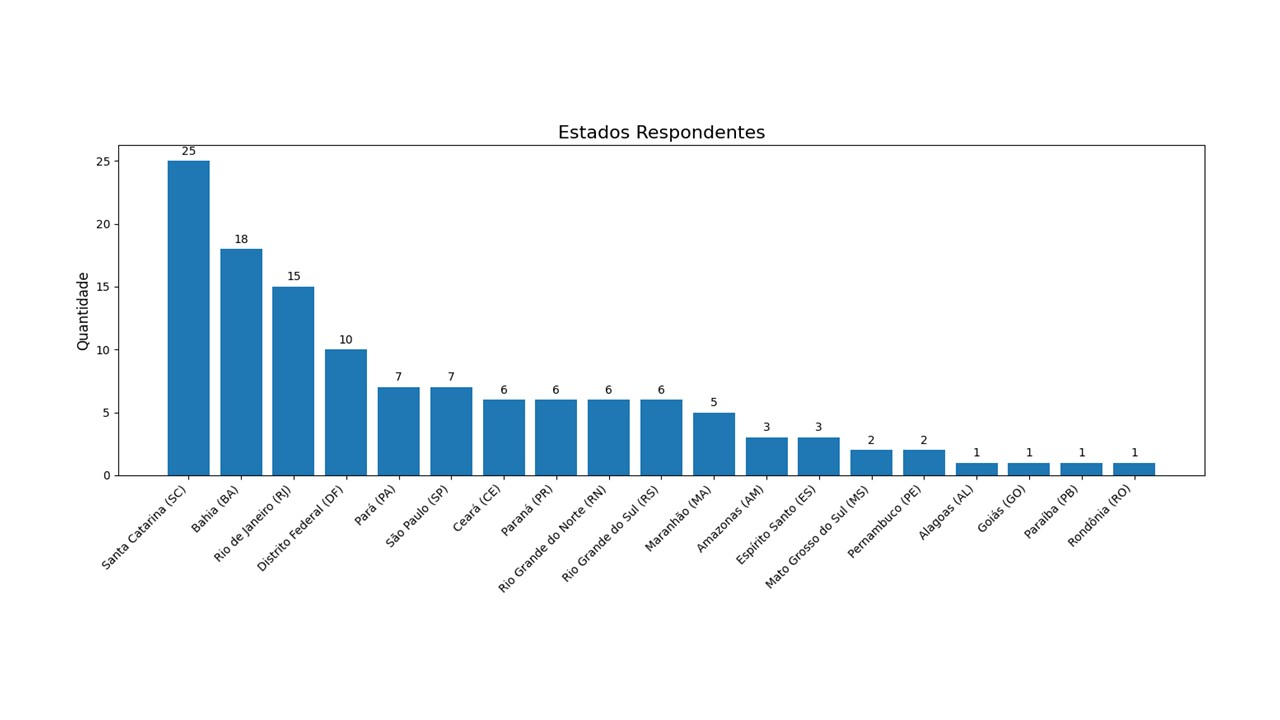
\includegraphics[keepaspectratio]{assets/Slide2.JPG}}

Quando analisado pelo recorte regional, o Nordeste apresentou a maior
adesão de respondentes.

\pandocbounded{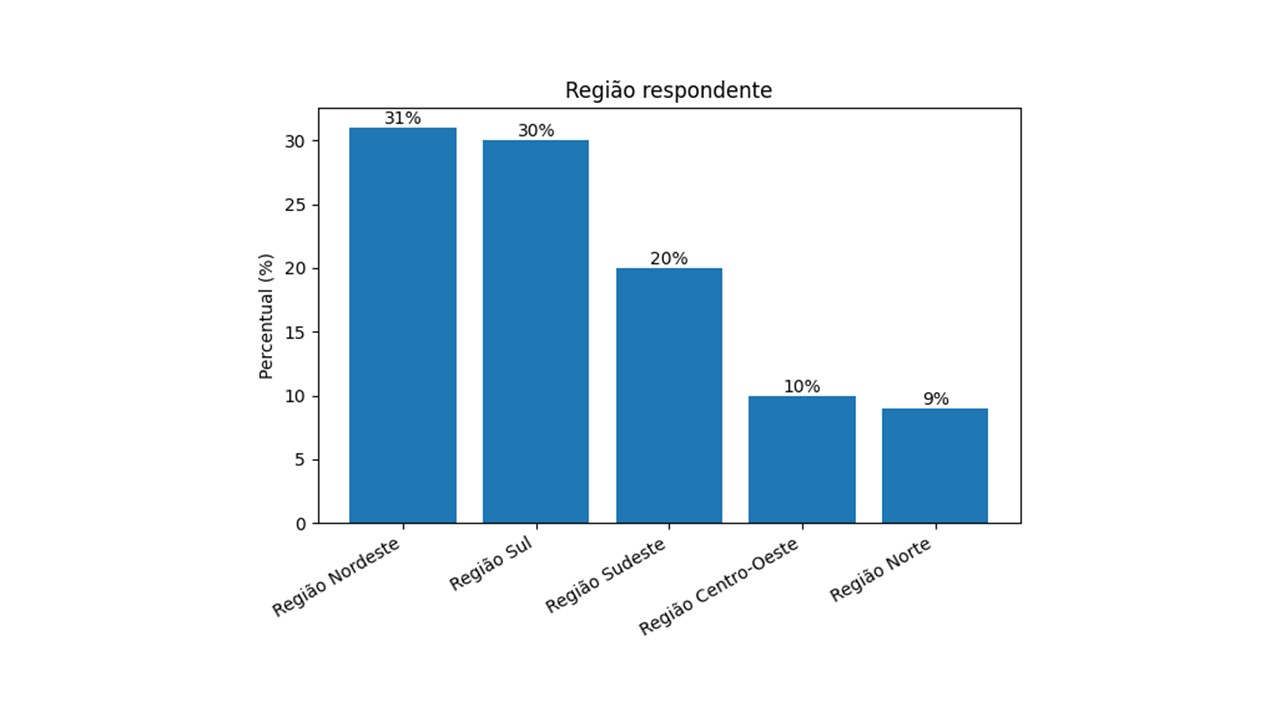
\includegraphics[keepaspectratio]{assets/Slide3.JPG}}

Pelo recorte de área de atuação organizacional, verifica-se que a
maioria pertence à área de gestão, meio ambiente e sustentabilidade e
operacional.

\pandocbounded{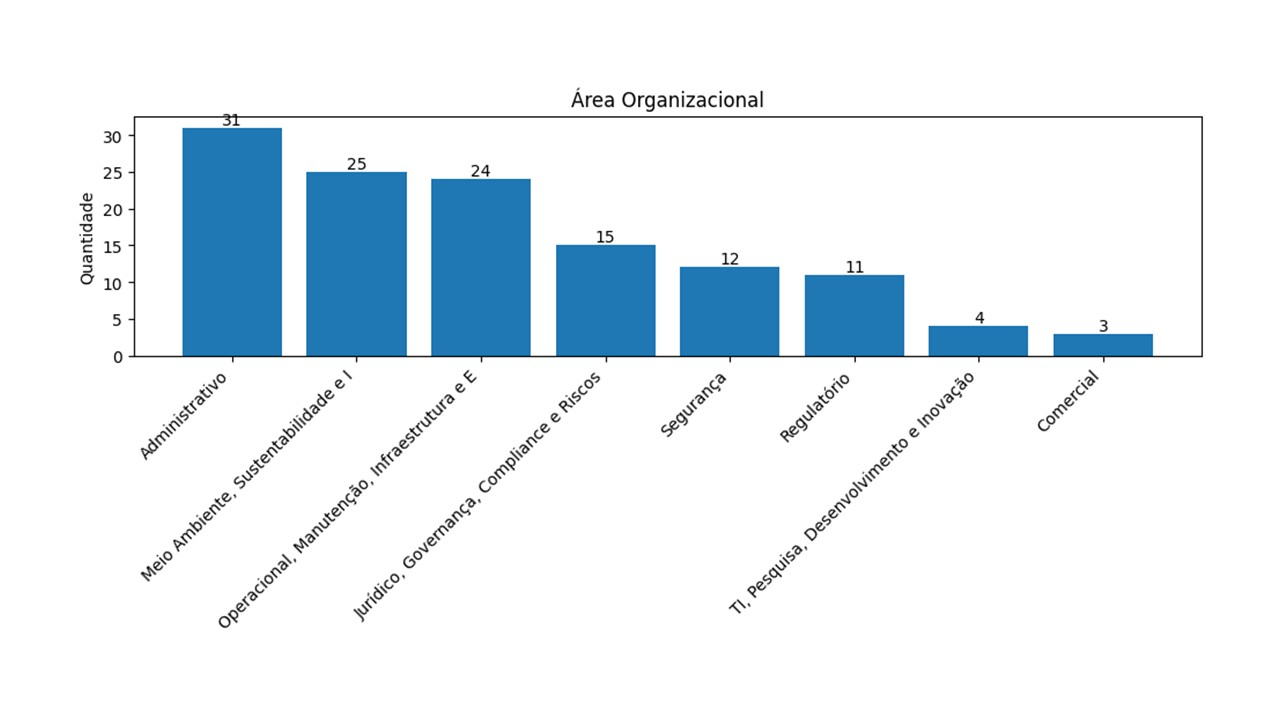
\includegraphics[keepaspectratio]{assets/Slide4.JPG}}

\section{Horizonte Temporal}\label{horizonte-temporal}

Os riscos foram avaliados considerando três horizontes temporais,
permitindo distinguir ameaças urgentes de tendências estruturais e
orientar ações de curto, médio e longo prazo:

\begin{itemize}
\item
  \textbf{Imediato (2025)} -- Riscos que requerem atenção e resposta
  imediata, exigindo capacidade de reação rápida e protocolos de
  contingência.
\item
  \textbf{Curto prazo (2026-2027)} -- Riscos emergentes que demandam
  planejamento estratégico, investimentos direcionados e ajustes
  regulatórios.
\item
  \textbf{Longo prazo (até 2035)} -- Riscos estratégicos que requerem
  visão de futuro, transformações estruturais e construção de
  resiliência institucional.
\end{itemize}

Essa abordagem temporal possibilita identificar não apenas os desafios
presentes, mas também antecipar cenários futuros, subsidiar o
planejamento de infraestrutura portuária de longo ciclo de maturação e
orientar políticas públicas que integrem respostas emergenciais, ajustes
táticos e transformações estratégicas do setor.

\section{Variáveis por Dimensão}\label{variuxe1veis-por-dimensuxe3o}

O questionário original contemplou um total de 76 variáveis distribuídas
em cinco dimensões de análise, proporcionando uma visão abrangente e
multicritérios dos riscos que afetam o setor portuário brasileiro. Essa
estrutura foi desenhada para capturar a complexidade e interdependência
dos riscos em diferentes níveis e dimensões da atividade portuária.

\begin{itemize}
\item
  \textbf{Dimensão Econômica}: 21 variáveis -- abrangem riscos
  relacionados à estabilidade financeira, endividamento, inflação,
  competitividade portuária, regulação e estabilidade macroeconômica,
  capturando desafios estruturais e conjunturais que afetam a
  viabilidade econômica das operações portuárias.
\item
  \textbf{Dimensão Ambiental}: 17 variáveis -- envolvem questões como
  mudanças climáticas, biodiversidade, poluição (atmosférica, hídrica e
  de sedimentos), desastres naturais, gerenciamento de resíduos,
  descarbonização do transporte marítimo e licenciamento ambiental,
  refletindo a crescente importância da sustentabilidade ambiental na
  gestão portuária.
\item
  \textbf{Dimensão Geopolítica}: 7 variáveis -- compreendem conflitos
  geoeconômicos, conflitos armados, violência em países de relação,
  terrorismo, ameaças biológicas/químicas/nucleares, alterações em
  sistemas terrestres e migração forçada, representando riscos externos
  e internacionais que podem impactar o comércio e a segurança
  portuária.
\item
  \textbf{Dimensão Social}: 15 variáveis -- abordam direitos humanos,
  pandemias, serviços públicos essenciais, acidentes, gestão de crises,
  recursos humanos capacitados, assédio no trabalho, desigualdades,
  participação social e adoção de novas tecnologias no ambiente laboral,
  destacando a importância do capital humano e das relações trabalhistas
  para a operação portuária.
\item
  \textbf{Dimensão Tecnológica}: 16 variáveis -- englobam riscos
  associados à inteligência artificial, tecnologias avançadas, segurança
  cibernética, privacidade, automação portuária, navios autônomos,
  tecnologias espaciais, integração de sistemas, desenvolvimento seguro
  de software e custo de implementação tecnológica, refletindo os
  desafios e oportunidades da transformação digital no setor portuário.
\end{itemize}

Essa estrutura multicritérios permite uma análise abrangente e integrada
dos riscos portuários, considerando diferentes perspectivas e
interdependências entre as dimensões analisadas. Cada variável foi
avaliada nos três horizontes temporais (imediato 2025, curto prazo
2026-2027 e longo prazo até 2035), totalizando 233 itens de coleta de
dados que capturam a evolução temporal da percepção dos riscos.

\section{Escala Likert e Tratamento
Estatístico}\label{escala-likert-e-tratamento-estatuxedstico}

\subsection{Natureza dos Dados}\label{natureza-dos-dados}

A coleta de dados utilizou uma escala Likert de 5 pontos para avaliar a
percepção dos gestores sobre os riscos portuários:

\begin{itemize}
\tightlist
\item
  1 - Risco muito baixo;- 2 - Risco baixo;- 3 - Risco moderado;- 4 -
  Risco alto;- 5 - Risco muito alto. \#\#\# Cálculo de Medidas de
  Tendência Central
\end{itemize}

A média foi calculada como a soma de todas as respostas dividida pelo
número total de respondentes para cada variável:

\[\bar{x} = \frac{\sum_{i=1}^{n} x_i}{n}\]

Onde:

\begin{itemize}
\item
  \(\bar{x}\) = média da variável;
\item
  \(x_i\) = valor da resposta do i-ésimo respondente (1 a 5);
\item
  \(n\) = número total de respondentes. Interpretação da média:
\item
  1,0 - 1,9: Percepção de risco muito baixo;- 2,0 - 2,9: Percepção de
  risco baixo;- 3,0 - 3,9: Percepção de risco moderado;- 4,0 - 4,9:
  Percepção de risco alto;- 5,0: Percepção de risco muito alto. A
  mediana representa o valor central quando todas as respostas são
  ordenadas. Para dados em escala Likert, a mediana é particularmente
  útil pois:
\item
  Não é afetada por valores extremos (outliers);- Representa a posição
  típica do grupo;- É mais robusta para distribuições assimétricas.
  Foram usadas as duas medidas pois fornecem uma visão complementar:
\item
  Média: Captura a intensidade geral das percepções;- Mediana: Indica a
  posição central e é resistente a extremos. \#\#\#\# Interpretação
  Conjunta
\item
  Média ≈ Mediana: Distribuição simétrica, consenso claro;- Média
  \textgreater{} Mediana: Concentração de respostas mais altas, alguns
  valores extremos elevados;- Média \textless{} Mediana: Concentração de
  respostas mais baixas, alguns valores extremos reduzidos. \#\#\#
  Análise por Dimensão
\end{itemize}

Para cada dimensão de risco (econômica, ambiental, social, tecnológica e
geopolítica), foram calculadas:

\begin{enumerate}
\def\labelenumi{\arabic{enumi}.}
\tightlist
\item
  Médias e medianas individuais para cada variável;2. Médias e medianas
  agregadas por dimensão;3. Desvio padrão para medir a dispersão das
  respostas;4. Frequências absolutas e relativas para cada ponto da
  escala. \#\#\# Validade Estatística
\end{enumerate}

A abordagem metodológica adotada segue as melhores práticas para análise
de dados Likert:

\begin{itemize}
\tightlist
\item
  Preservação da natureza ordinal dos dados;- Uso adequado de
  estatísticas descritivas;- Complementaridade entre medidas para
  análise;- Transparência nos critérios de interpretação. \#\# Abordagem
  Analítica
\end{itemize}

\begin{enumerate}
\def\labelenumi{\arabic{enumi}.}
\tightlist
\item
  Tratamento dos dados: limpeza, padronização e consolidação das
  respostas.
\item
  Construção de indicadores: cálculo de percentuais por nível de risco e
  mediana por horizonte temporal.
\item
  Visualização e interpretação: elaboração de gráficos comparativos e
  sínteses interpretativas.
\end{enumerate}

\subsection{Análise Estatística de Dispersão
Temporal}\label{anuxe1lise-estatuxedstica-de-dispersuxe3o-temporal}

Para avaliar a evolução percebida dos riscos entre horizontes temporais,
foi estruturado um pipeline estatístico de dispersão com manutenção
integral dos 57 pares curto vs.~longo prazo.

\subsubsection{Metodologia de Correspondência
Temporal}\label{metodologia-de-corresponduxeancia-temporal}

\begin{itemize}
\tightlist
\item
  Identificação de pares temporais: correspondência automática por
  código da variável entre curto prazo (2026-2027) e longo prazo (até
  2035).
\item
  Extração de estatísticas: para cada par calculamos mediana, intervalo
  interquartil (IQR), delta temporal com sinal (mediana longo - mediana
  curto) e delta absoluto.
\item
  Classificação de tendência:
\end{itemize}

\begin{enumerate}
\def\labelenumi{\arabic{enumi}.}
\tightlist
\item
  Delta positivo: risco aumenta no longo prazo, ou seja, tendência de
  agravamento;2. Delta negativo: risco diminui no longo prazo, ou seja,
  tendência de melhoria;3. Delta zero: risco estável entre os
  horizontes, equivalente à estabilidade.
\end{enumerate}

\subsubsection{Interpretação
Estatística}\label{interpretauxe7uxe3o-estatuxedstica}

\begin{itemize}
\tightlist
\item
  Correlação temporal: coeficiente de Pearson calculado para medir a
  persistência entre horizontes.
\item
  Análise de deltas: o delta com sinal identifica agravamentos ou
  melhorias; o delta absoluto resume a magnitude da mudança.
\item
  Quadrantes estratégicos: contagens e percentuais por quadrante
  alimentam tanto o gráfico quanto a narrativa do relatório.
\end{itemize}

\bookmarksetup{startatroot}

\chapter{Riscos Globais Portuários}\label{riscos-globais-portuuxe1rios}

\section{Riscos por dimensão}\label{riscos-por-dimensuxe3o}

\subsection{Riscos econômicos}\label{riscos-econuxf4micos}

\textbf{Tabela 1: Análise Estatística dos Riscos Econômicos por
Horizonte Temporal}

\begin{longtable}[]{@{}
  >{\raggedright\arraybackslash}p{(\linewidth - 16\tabcolsep) * \real{0.1111}}
  >{\raggedright\arraybackslash}p{(\linewidth - 16\tabcolsep) * \real{0.1111}}
  >{\raggedright\arraybackslash}p{(\linewidth - 16\tabcolsep) * \real{0.1111}}
  >{\raggedright\arraybackslash}p{(\linewidth - 16\tabcolsep) * \real{0.1111}}
  >{\raggedright\arraybackslash}p{(\linewidth - 16\tabcolsep) * \real{0.1111}}
  >{\raggedright\arraybackslash}p{(\linewidth - 16\tabcolsep) * \real{0.1111}}
  >{\raggedright\arraybackslash}p{(\linewidth - 16\tabcolsep) * \real{0.1111}}
  >{\raggedright\arraybackslash}p{(\linewidth - 16\tabcolsep) * \real{0.1111}}
  >{\raggedright\arraybackslash}p{(\linewidth - 16\tabcolsep) * \real{0.1111}}@{}}
\toprule\noalign{}
\begin{minipage}[b]{\linewidth}\raggedright
Risco
\end{minipage} & \begin{minipage}[b]{\linewidth}\raggedright
Período
\end{minipage} & \begin{minipage}[b]{\linewidth}\raggedright
Média
\end{minipage} & \begin{minipage}[b]{\linewidth}\raggedright
Mediana
\end{minipage} & \begin{minipage}[b]{\linewidth}\raggedright
Moda
\end{minipage} & \begin{minipage}[b]{\linewidth}\raggedright
Desvio Padrão
\end{minipage} & \begin{minipage}[b]{\linewidth}\raggedright
\% Risco Alto
\end{minipage} & \begin{minipage}[b]{\linewidth}\raggedright
\% Risco Baixo
\end{minipage} & \begin{minipage}[b]{\linewidth}\raggedright
Nível de Risco
\end{minipage} \\
\midrule\noalign{}
\endhead
\bottomrule\noalign{}
\endlastfoot
Especulação e crise no mercado de ativos financeiros & Imediato (2025) &
2,66 & 3 & 1 & 1,32 & 28,0 & 45,6 & Moderado \\
& Curto Prazo (2026--2027) & 2,81 & 3 & 3 & 1,04 & 24,8 & 36,8 &
Moderado \\
& Longo Prazo (2035) & 2,93 & 3 & 3 & 1,21 & 32,0 & 37,6 &
Moderado-alto \\
Aumento da inflação & Imediato (2025) & 2,84 & 3 & 3 & 1,24 & 32,0 &
36,8 & Moderado-alto \\
& Curto Prazo (2026--2027) & 3,17 & 3 & 3 & 1,11 & 38,4 & 27,2 &
Moderado-alto \\
& Longo Prazo (2035) & 3,30 & 3 & 3 & 1,09 & 43,2 & 24,8 &
Moderado-alto \\
Dificuldades de financiamento para investimento & Imediato (2025) & 2,70
& 3 & 3 & 1,31 & 27,2 & 44,0 & Moderado \\
& Curto Prazo (2026--2027) & 3,01 & 3 & 3 & 1,23 & 34,4 & 33,6 &
Moderado-alto \\
& Longo Prazo (2035) & 3,16 & 3 & 3 & 1,19 & 39,2 & 28,8 &
Moderado-alto \\
Riscos reputacionais & Imediato (2025) & 2,60 & 3 & 3 & 1,30 & 23,2 &
46,4 & Moderado \\
& Curto Prazo (2026--2027) & 2,85 & 3 & 3 & 1,24 & 29,6 & 36,0 &
Moderado \\
& Longo Prazo (2035) & 2,86 & 3 & 3 & 1,23 & 29,6 & 38,4 & Moderado \\
Risco de competitividade portuária & Imediato (2025) & 2,83 & 3 & 4 &
1,29 & 35,2 & 42,4 & Moderado-alto \\
& Curto Prazo (2026--2027) & 3,19 & 3 & 3 & 1,17 & 40,8 & 28,8 &
Moderado-alto \\
& Longo Prazo (2035) & 3,42 & 4 & 4 & 1,25 & 51,2 & 21,6 & Crítico \\
Aumento de impostos & Imediato (2025) & 3,11 & 3 & 4 & 1,36 & 45,6 &
32,8 & Moderado-alto \\
& Curto Prazo (2026--2027) & 3,34 & 4 & 4 & 1,19 & 51,2 & 27,2 &
Crítico \\
& Longo Prazo (2035) & 3,45 & 4 & 4 & 1,19 & 52,0 & 24,0 & Crítico \\
Instabilidade política & Imediato (2025) & 3,42 & 4 & 5 & 1,36 & 50,4 &
26,4 & Crítico \\
& Curto Prazo (2026--2027) & 3,74 & 4 & 4 & 1,08 & 60,8 & 12,8 &
Crítico \\
& Longo Prazo (2035) & 3,62 & 4 & 3 & 1,08 & 53,6 & 15,2 & Crítico \\
Excesso regulatório & Imediato (2025) & 3,26 & 3 & 3 & 1,29 & 46,4 &
27,2 & Moderado-alto \\
& Curto Prazo (2026--2027) & 3,49 & 4 & 4 & 1,09 & 53,6 & 18,4 &
Crítico \\
& Longo Prazo (2035) & 3,54 & 4 & 4 & 1,15 & 52,8 & 20,8 & Crítico \\
Déficit regulatório & Imediato (2025) & 2,55 & 3 & 1 & 1,30 & 24,8 &
49,6 & Moderado \\
& Curto Prazo (2026--2027) & 2,75 & 3 & 3 & 1,20 & 27,2 & 40,8 &
Moderado \\
& Longo Prazo (2035) & 2,89 & 3 & 3 & 1,25 & 33,6 & 39,2 &
Moderado-alto \\
Desemprego & Imediato (2025) & 2,42 & 2 & 1 & 1,23 & 22,4 & 56,8 &
Moderado \\
& Curto Prazo (2026--2027) & 2,79 & 3 & 3 & 1,20 & 27,2 & 40,8 &
Moderado \\
& Longo Prazo (2035) & 2,99 & 3 & 3 & 1,18 & 32,0 & 34,4 &
Moderado-alto \\
Corrupção & Imediato (2025) & 3,17 & 3 & 5 & 1,46 & 45,6 & 36,0 &
Moderado-alto \\
& Curto Prazo (2026--2027) & 3,31 & 3 & 5 & 1,31 & 47,2 & 29,6 &
Moderado-alto \\
& Longo Prazo (2035) & 3,39 & 3 & 3 & 1,29 & 48,0 & 24,0 &
Moderado-alto \\
Falhas em cadeias de suprimentos & Imediato (2025) & 2,97 & 3 & 4 & 1,40
& 40,0 & 38,4 & Moderado-alto \\
& Curto Prazo (2026--2027) & 3,29 & 4 & 4 & 1,20 & 50,4 & 28,0 &
Crítico \\
& Longo Prazo (2035) & 3,30 & 3 & 3 & 1,17 & 44,8 & 24,0 &
Moderado-alto \\
Ação do crime organizado & Imediato (2025) & 3,04 & 3 & 3 & 1,36 & 36,0
& 36,0 & Moderado-alto \\
& Curto Prazo (2026--2027) & 3,19 & 3 & 3 & 1,28 & 42,4 & 32,8 &
Moderado-alto \\
& Longo Prazo (2035) & 3,28 & 3 & 3 & 1,27 & 44,8 & 26,4 &
Moderado-alto \\
\end{longtable}

\emph{Fonte: elaboração própria}

\subsection{Riscos ambientais}\label{riscos-ambientais}

\textbf{Tabela 2: Análise Estatística dos Riscos Ambientais por
Horizonte Temporal}

\begin{longtable}[]{@{}
  >{\raggedright\arraybackslash}p{(\linewidth - 16\tabcolsep) * \real{0.0619}}
  >{\raggedright\arraybackslash}p{(\linewidth - 16\tabcolsep) * \real{0.0928}}
  >{\raggedright\arraybackslash}p{(\linewidth - 16\tabcolsep) * \real{0.0722}}
  >{\raggedright\arraybackslash}p{(\linewidth - 16\tabcolsep) * \real{0.0928}}
  >{\raggedright\arraybackslash}p{(\linewidth - 16\tabcolsep) * \real{0.0619}}
  >{\raggedright\arraybackslash}p{(\linewidth - 16\tabcolsep) * \real{0.1546}}
  >{\raggedright\arraybackslash}p{(\linewidth - 16\tabcolsep) * \real{0.1443}}
  >{\raggedright\arraybackslash}p{(\linewidth - 16\tabcolsep) * \real{0.1546}}
  >{\raggedright\arraybackslash}p{(\linewidth - 16\tabcolsep) * \real{0.1649}}@{}}
\toprule\noalign{}
\begin{minipage}[b]{\linewidth}\raggedright
Risco
\end{minipage} & \begin{minipage}[b]{\linewidth}\raggedright
Período
\end{minipage} & \begin{minipage}[b]{\linewidth}\raggedright
Média
\end{minipage} & \begin{minipage}[b]{\linewidth}\raggedright
Mediana
\end{minipage} & \begin{minipage}[b]{\linewidth}\raggedright
Moda
\end{minipage} & \begin{minipage}[b]{\linewidth}\raggedright
Desvio Padrão
\end{minipage} & \begin{minipage}[b]{\linewidth}\raggedright
\% Risco Alto
\end{minipage} & \begin{minipage}[b]{\linewidth}\raggedright
\% Risco Baixo
\end{minipage} & \begin{minipage}[b]{\linewidth}\raggedright
Nível de Risco
\end{minipage} \\
\midrule\noalign{}
\endhead
\bottomrule\noalign{}
\endlastfoot
Perda de biodiversidade e colapso de ecossistemas & Imediato (2025) &
2,22 & 2 & 1 & 1,26 & 16,0 & 60,8 & Moderado \\
& Curto Prazo (2026--2027) & 2,60 & 3 & 1 & 1,26 & 26,4 & 47,2 &
Moderado \\
& Longo Prazo (2035) & 3,11 & 3 & 3 & 1,36 & 41,6 & 33,6 &
Moderado-alto \\
Introdução de espécies exóticas e agentes patogênicos & Imediato (2025)
& 2,43 & 2 & 1 & 1,27 & 24,0 & 58,4 & Moderado \\
& Curto Prazo (2026--2027) & 2,67 & 2 & 2 & 1,26 & 27,2 & 51,2 &
Moderado \\
& Longo Prazo (2035) & 2,95 & 3 & 3 & 1,28 & 35,2 & 39,2 &
Moderado-alto \\
Poluição atmosférica & Imediato (2025) & 2,45 & 2 & 3 & 1,21 & 18,4 &
51,2 & Moderado \\
& Curto Prazo (2026--2027) & 2,72 & 3 & 3 & 1,18 & 27,2 & 43,2 &
Moderado \\
& Longo Prazo (2035) & 2,99 & 3 & 3 & 1,23 & 36,0 & 36,8 &
Moderado-alto \\
Ruídos e vibrações & Imediato (2025) & 2,26 & 2 & 1 & 1,25 & 17,6 & 60,8
& Moderado \\
& Curto Prazo (2026--2027) & 2,42 & 2 & 1 & 1,23 & 20,8 & 53,6 &
Moderado \\
& Longo Prazo (2035) & 2,62 & 3 & 1 & 1,28 & 27,2 & 48,8 & Moderado \\
Gerenciamento inadequado de resíduos sólidos & Imediato (2025) & 2,32 &
2 & 1 & 1,34 & 19,2 & 57,6 & Moderado \\
& Curto Prazo (2026--2027) & 2,52 & 2 & 1 & 1,34 & 26,4 & 52,8 &
Moderado \\
& Longo Prazo (2035) & 2,72 & 3 & 1 & 1,35 & 32,0 & 48,0 &
Moderado-alto \\
Desmatamento & Imediato (2025) & 2,01 & 2 & 1 & 1,20 & 12,8 & 68,0 &
Moderado \\
& Curto Prazo (2026--2027) & 2,26 & 2 & 1 & 1,24 & 17,6 & 60,0 &
Moderado \\
& Longo Prazo (2035) & 2,60 & 3 & 1 & 1,36 & 28,0 & 47,2 & Moderado \\
Licenciamento ambiental & Imediato (2025) & 2,62 & 2 & 1 & 1,47 & 28,8 &
50,4 & Moderado \\
& Curto Prazo (2026--2027) & 2,82 & 3 & 3 & 1,37 & 32,8 & 43,2 &
Moderado-alto \\
& Longo Prazo (2035) & 3,07 & 3 & 5 & 1,45 & 43,2 & 37,6 &
Moderado-alto \\
Descarbonização do transporte marítimo & Imediato (2025) & 2,30 & 2 & 2
& 1,19 & 14,4 & 63,2 & Moderado \\
& Curto Prazo (2026--2027) & 2,61 & 3 & 2 & 1,16 & 21,6 & 49,6 &
Moderado \\
& Longo Prazo (2035) & 3,04 & 3 & 3 & 1,36 & 37,6 & 37,6 &
Moderado-alto \\
Baixa educação ambiental & Imediato (2025) & 2,58 & 2 & 2 & 1,25 & 21,6
& 52,0 & Moderado \\
& Curto Prazo (2026--2027) & 2,75 & 3 & 3 & 1,16 & 23,2 & 42,4 &
Moderado \\
& Longo Prazo (2035) & 2,98 & 3 & 3 & 1,32 & 36,0 & 38,4 &
Moderado-alto \\
Eventos que impactam acessos e operações portuárias & Imediato (2025) &
2,52 & 2 & 1 & 1,39 & 24,0 & 56,0 & Moderado \\
& Curto Prazo (2026--2027) & 2,74 & 3 & 2 & 1,33 & 32,0 & 47,2 &
Moderado-alto \\
& Longo Prazo (2035) & 3,04 & 3 & 3 & 1,32 & 36,8 & 36,8 &
Moderado-alto \\
Mudanças climáticas & Imediato (2025) & 2,62 & 2 & 2 & 1,29 & 26,4 &
51,2 & Moderado \\
& Curto Prazo (2026--2027) & 3,01 & 3 & 3 & 1,25 & 36,8 & 37,6 &
Moderado-alto \\
& Longo Prazo (2035) & 3,43 & 4 & 5 & 1,35 & 52,0 & 26,4 & Crítico \\
Crise de recursos naturais (água e alimentos) & Imediato (2025) & 2,40 &
2 & 1 & 1,32 & 22,4 & 61,6 & Moderado \\
& Curto Prazo (2026--2027) & 2,84 & 3 & 2 & 1,27 & 34,4 & 44,8 &
Moderado-alto \\
& Longo Prazo (2035) & 3,28 & 3 & 4 & 1,32 & 48,8 & 30,4 &
Moderado-alto \\
Desastres naturais não climáticos & Imediato (2025) & 2,09 & 2 & 1 &
1,33 & 15,2 & 71,2 & Moderado \\
& Curto Prazo (2026--2027) & 2,29 & 2 & 1 & 1,29 & 21,6 & 64,0 &
Moderado \\
& Longo Prazo (2035) & 2,57 & 2 & 1 & 1,35 & 24,8 & 53,6 & Moderado \\
Elevação do nível do mar e erosão costeira & Imediato (2025) & 2,21 & 2
& 1 & 1,29 & 19,2 & 64,8 & Moderado \\
& Curto Prazo (2026--2027) & 2,55 & 2 & 1 & 1,29 & 25,6 & 52,8 &
Moderado \\
& Longo Prazo (2035) & 2,98 & 3 & 2 & 1,38 & 37,6 & 43,2 &
Moderado-alto \\
Poluição da água e sedimentos portuários & Imediato (2025) & 2,47 & 2 &
1 & 1,34 & 24,0 & 58,4 & Moderado \\
& Curto Prazo (2026--2027) & 2,72 & 2 & 2 & 1,29 & 32,0 & 50,4 &
Moderado \\
& Longo Prazo (2035) & 3,02 & 3 & 4 & 1,31 & 41,6 & 40,0 &
Moderado-alto \\
Movimentação de produtos perigosos & Imediato (2025) & 2,45 & 2 & 1 &
1,39 & 24,0 & 60,0 & Moderado \\
& Curto Prazo (2026--2027) & 2,62 & 2 & 2 & 1,32 & 27,2 & 52,8 &
Moderado \\
& Longo Prazo (2035) & 2,86 & 3 & 3 & 1,32 & 29,6 & 40,0 & Moderado \\
Agentes patogênicos e saneamento inadequado & Imediato (2025) & 2,46 & 2
& 1 & 1,41 & 27,2 & 56,8 & Moderado \\
& Curto Prazo (2026--2027) & 2,60 & 2 & 2 & 1,30 & 29,6 & 52,0 &
Moderado \\
& Longo Prazo (2035) & 2,70 & 3 & 2 & 1,30 & 30,4 & 48,0 &
Moderado-alto \\
\end{longtable}

\emph{Fonte: elaboração própria}

\subsection{Riscos geopolíticos}\label{riscos-geopoluxedticos}

\textbf{Tabela 3: Análise Estatística dos Riscos Geopolíticos por
Horizonte Temporal}

\begin{longtable}[]{@{}
  >{\raggedright\arraybackslash}p{(\linewidth - 16\tabcolsep) * \real{0.0619}}
  >{\raggedright\arraybackslash}p{(\linewidth - 16\tabcolsep) * \real{0.0928}}
  >{\raggedright\arraybackslash}p{(\linewidth - 16\tabcolsep) * \real{0.0722}}
  >{\raggedright\arraybackslash}p{(\linewidth - 16\tabcolsep) * \real{0.0928}}
  >{\raggedright\arraybackslash}p{(\linewidth - 16\tabcolsep) * \real{0.0619}}
  >{\raggedright\arraybackslash}p{(\linewidth - 16\tabcolsep) * \real{0.1546}}
  >{\raggedright\arraybackslash}p{(\linewidth - 16\tabcolsep) * \real{0.1443}}
  >{\raggedright\arraybackslash}p{(\linewidth - 16\tabcolsep) * \real{0.1546}}
  >{\raggedright\arraybackslash}p{(\linewidth - 16\tabcolsep) * \real{0.1649}}@{}}
\toprule\noalign{}
\begin{minipage}[b]{\linewidth}\raggedright
Risco
\end{minipage} & \begin{minipage}[b]{\linewidth}\raggedright
Período
\end{minipage} & \begin{minipage}[b]{\linewidth}\raggedright
Média
\end{minipage} & \begin{minipage}[b]{\linewidth}\raggedright
Mediana
\end{minipage} & \begin{minipage}[b]{\linewidth}\raggedright
Moda
\end{minipage} & \begin{minipage}[b]{\linewidth}\raggedright
Desvio Padrão
\end{minipage} & \begin{minipage}[b]{\linewidth}\raggedright
\% Risco Alto
\end{minipage} & \begin{minipage}[b]{\linewidth}\raggedright
\% Risco Baixo
\end{minipage} & \begin{minipage}[b]{\linewidth}\raggedright
Nível de Risco
\end{minipage} \\
\midrule\noalign{}
\endhead
\bottomrule\noalign{}
\endlastfoot
Liberação intencional ou acidental de contaminante biológico, químico,
nuclear ou radiológico & Imediato (2025) & 2,17 & 2 & 1 & 1,34 & 16,8 &
68,0 & Moderado \\
& Curto Prazo (2026--2027) & 2,36 & 2 & 1 & 1,31 & 19,2 & 62,4 &
Moderado \\
& Longo Prazo (2035) & 2,64 & 3 & 1 & 1,39 & 24,8 & 49,6 & Moderado \\
Alterações em condições de sistemas terrestres & Imediato (2025) & 2,26
& 2 & 1 & 1,37 & 20,8 & 64,0 & Moderado \\
& Curto Prazo (2026--2027) & 2,56 & 2 & 1 & 1,40 & 29,6 & 56,8 &
Moderado \\
& Longo Prazo (2035) & 2,85 & 3 & 1 & 1,39 & 36,0 & 44,0 &
Moderado-alto \\
Conflitos geoeconômicos (sanções, bloqueios e restrições) & Imediato
(2025) & 3,27 & 3 & 4 & 1,30 & 46,4 & 29,6 & Moderado-alto \\
& Curto Prazo (2026--2027) & 3,49 & 4 & 4 & 1,19 & 56,0 & 24,0 &
Crítico \\
& Longo Prazo (2035) & 3,58 & 4 & 4 & 1,17 & 60,0 & 21,6 & Crítico \\
Conflitos armados entre nações & Imediato (2025) & 2,66 & 2 & 1 & 1,46 &
31,2 & 52,8 & Moderado \\
& Curto Prazo (2026--2027) & 2,90 & 3 & 3 & 1,42 & 32,8 & 39,2 &
Moderado-alto \\
& Longo Prazo (2035) & 3,10 & 3 & 4 & 1,41 & 44,0 & 35,2 &
Moderado-alto \\
Violência aberta em países de relação (greves, conflitos internos,
golpes, insegurança pública) & Imediato (2025) & 2,63 & 2 & 1 & 1,38 &
28,0 & 52,8 & Moderado \\
& Curto Prazo (2026--2027) & 2,90 & 3 & 2 & 1,33 & 33,6 & 44,0 &
Moderado-alto \\
& Longo Prazo (2035) & 3,07 & 3 & 3 & 1,31 & 37,6 & 36,0 &
Moderado-alto \\
Terrorismo & Imediato (2025) & 2,53 & 2 & 1 & 1,44 & 30,4 & 58,4 &
Moderado \\
& Curto Prazo (2026--2027) & 2,77 & 2 & 2 & 1,40 & 32,8 & 50,4 &
Moderado \\
& Longo Prazo (2035) & 3,01 & 3 & 2 & 1,42 & 40,8 & 42,4 &
Moderado-alto \\
Migração ou deslocamento forçado & Imediato (2025) & 2,40 & 2 & 1 & 1,38
& 24,0 & 59,2 & Moderado \\
& Curto Prazo (2026--2027) & 2,70 & 2 & 1 & 1,40 & 32,8 & 50,4 &
Moderado \\
& Longo Prazo (2035) & 2,90 & 3 & 4 & 1,31 & 36,8 & 41,6 &
Moderado-alto \\
\end{longtable}

\emph{Fonte: elaboração própria}

\subsection{Riscos sociais}\label{riscos-sociais}

\textbf{Tabela 4: Análise Estatística dos Riscos Sociais por Horizonte
Temporal}

\begin{longtable}[]{@{}
  >{\raggedright\arraybackslash}p{(\linewidth - 16\tabcolsep) * \real{0.0619}}
  >{\raggedright\arraybackslash}p{(\linewidth - 16\tabcolsep) * \real{0.0928}}
  >{\raggedright\arraybackslash}p{(\linewidth - 16\tabcolsep) * \real{0.0722}}
  >{\raggedright\arraybackslash}p{(\linewidth - 16\tabcolsep) * \real{0.0928}}
  >{\raggedright\arraybackslash}p{(\linewidth - 16\tabcolsep) * \real{0.0619}}
  >{\raggedright\arraybackslash}p{(\linewidth - 16\tabcolsep) * \real{0.1546}}
  >{\raggedright\arraybackslash}p{(\linewidth - 16\tabcolsep) * \real{0.1443}}
  >{\raggedright\arraybackslash}p{(\linewidth - 16\tabcolsep) * \real{0.1546}}
  >{\raggedright\arraybackslash}p{(\linewidth - 16\tabcolsep) * \real{0.1649}}@{}}
\toprule\noalign{}
\begin{minipage}[b]{\linewidth}\raggedright
Risco
\end{minipage} & \begin{minipage}[b]{\linewidth}\raggedright
Período
\end{minipage} & \begin{minipage}[b]{\linewidth}\raggedright
Média
\end{minipage} & \begin{minipage}[b]{\linewidth}\raggedright
Mediana
\end{minipage} & \begin{minipage}[b]{\linewidth}\raggedright
Moda
\end{minipage} & \begin{minipage}[b]{\linewidth}\raggedright
Desvio Padrão
\end{minipage} & \begin{minipage}[b]{\linewidth}\raggedright
\% Risco Alto
\end{minipage} & \begin{minipage}[b]{\linewidth}\raggedright
\% Risco Baixo
\end{minipage} & \begin{minipage}[b]{\linewidth}\raggedright
Nível de Risco
\end{minipage} \\
\midrule\noalign{}
\endhead
\bottomrule\noalign{}
\endlastfoot
Ameaças aos direitos humanos e/ou às liberdades individuais ou de grupo
& Imediato (2025) & 2,36 & 2 & 1 & 1,39 & 20,8 & 59,2 & Moderado \\
& Curto Prazo (2026--2027) & 2,60 & 2 & 1 & 1,36 & 26,4 & 51,2 &
Moderado \\
& Longo Prazo (2035) & 2,82 & 3 & 3 & 1,38 & 32,8 & 41,6 &
Moderado-alto \\
Falta de recursos humanos capacitados no setor portuário & Imediato
(2025) & 2,81 & 3 & 3 & 1,18 & 27,2 & 40,8 & Moderado \\
& Curto Prazo (2026--2027) & 3,06 & 3 & 3 & 1,18 & 35,2 & 31,2 &
Moderado-alto \\
& Longo Prazo (2035) & 3,12 & 3 & 3 & 1,30 & 39,2 & 31,2 &
Moderado-alto \\
Assédio moral e sexual no ambiente de trabalho & Imediato (2025) & 2,46
& 2 & 1 & 1,27 & 19,2 & 53,6 & Moderado \\
& Curto Prazo (2026--2027) & 2,55 & 2 & 3 & 1,21 & 20,0 & 50,4 &
Moderado \\
& Longo Prazo (2035) & 2,46 & 2 & 1 & 1,27 & 21,6 & 52,8 & Moderado \\
Desigualdades raciais, étnicas e de gênero & Imediato (2025) & 2,36 & 2
& 3 & 1,17 & 14,4 & 53,6 & Moderado \\
& Curto Prazo (2026--2027) & 2,43 & 2 & 3 & 1,19 & 17,6 & 52,8 &
Moderado \\
& Longo Prazo (2035) & 2,32 & 2 & 1 & 1,25 & 18,4 & 57,6 & Moderado \\
Falta de participação social & Imediato (2025) & 2,36 & 2 & 1 & 1,23 &
16,8 & 57,6 & Moderado \\
& Curto Prazo (2026--2027) & 2,45 & 2 & 1 & 1,25 & 19,2 & 52,8 &
Moderado \\
& Longo Prazo (2035) & 2,47 & 2 & 3 & 1,22 & 19,2 & 51,2 & Moderado \\
Maior uso de tecnologias (IA, mecanização e robotização) & Imediato
(2025) & 2,63 & 3 & 3 & 1,29 & 23,2 & 48,0 & Moderado \\
& Curto Prazo (2026--2027) & 2,92 & 3 & 3 & 1,32 & 35,2 & 40,8 &
Moderado-alto \\
& Longo Prazo (2035) & 3,22 & 3 & 5 & 1,49 & 47,2 & 35,2 &
Moderado-alto \\
Ausência do Estado junto às populações próximas aos portos & Imediato
(2025) & 2,78 & 3 & 3 & 1,26 & 26,4 & 43,2 & Moderado \\
& Curto Prazo (2026--2027) & 2,92 & 3 & 3 & 1,22 & 31,2 & 39,2 &
Moderado-alto \\
& Longo Prazo (2035) & 3,05 & 3 & 3 & 1,30 & 36,8 & 37,6 &
Moderado-alto \\
Pandemias ou epidemias de rápida disseminação & Imediato (2025) & 2,36 &
2 & 1 & 1,37 & 21,6 & 59,2 & Moderado \\
& Curto Prazo (2026--2027) & 2,82 & 3 & 2 & 1,23 & 28,8 & 47,2 &
Moderado \\
& Longo Prazo (2035) & 3,12 & 3 & 3 & 1,18 & 37,6 & 32,8 &
Moderado-alto \\
Insuficiência de serviços públicos essenciais & Imediato (2025) & 2,71 &
3 & 2 & 1,29 & 28,0 & 48,0 & Moderado \\
& Curto Prazo (2026--2027) & 2,93 & 3 & 2 & 1,20 & 33,6 & 42,4 &
Moderado-alto \\
& Longo Prazo (2035) & 3,13 & 3 & 3 & 1,22 & 40,8 & 32,8 &
Moderado-alto \\
Impactos geopolíticos & Imediato (2025) & 2,61 & 2 & 1 & 1,36 & 28,0 &
52,0 & Moderado \\
& Curto Prazo (2026--2027) & 2,95 & 3 & 4 & 1,33 & 38,4 & 40,0 &
Moderado-alto \\
& Longo Prazo (2035) & 3,20 & 3 & 4 & 1,31 & 48,0 & 32,0 &
Moderado-alto \\
Acidentes rodoviários e ferroviários em áreas portuárias & Imediato
(2025) & 2,61 & 2 & 1 & 1,33 & 24,0 & 50,4 & Moderado \\
& Curto Prazo (2026--2027) & 2,80 & 3 & 3 & 1,23 & 28,8 & 41,6 &
Moderado \\
& Longo Prazo (2035) & 2,86 & 3 & 3 & 1,27 & 33,6 & 40,8 &
Moderado-alto \\
Acidentes nas operações portuárias & Imediato (2025) & 2,77 & 3 & 3 &
1,36 & 30,4 & 44,8 & Moderado \\
& Curto Prazo (2026--2027) & 2,88 & 3 & 2 & 1,25 & 33,6 & 43,2 &
Moderado-alto \\
& Longo Prazo (2035) & 2,87 & 3 & 3 & 1,34 & 34,4 & 40,8 &
Moderado-alto \\
Falhas na gestão de crises e resposta a emergências & Imediato (2025) &
2,68 & 3 & 3 & 1,29 & 26,4 & 44,8 & Moderado \\
& Curto Prazo (2026--2027) & 2,82 & 3 & 3 & 1,19 & 28,0 & 38,4 &
Moderado \\
& Longo Prazo (2035) & 2,87 & 3 & 3 & 1,26 & 31,2 & 38,4 &
Moderado-alto \\
Falhas no controle interno (fraudes ou corrupção) & Imediato (2025) &
2,60 & 3 & 1 & 1,38 & 26,4 & 48,8 & Moderado \\
& Curto Prazo (2026--2027) & 2,75 & 3 & 3 & 1,34 & 29,6 & 45,6 &
Moderado \\
& Longo Prazo (2035) & 2,86 & 3 & 3 & 1,40 & 34,4 & 41,6 &
Moderado-alto \\
Instabilidade regulatória e excesso de judicialização & Imediato (2025)
& 2,94 & 3 & 3 & 1,34 & 34,4 & 36,8 & Moderado \\
& Curto Prazo (2026--2027) & 3,06 & 3 & 3 & 1,29 & 38,4 & 36,0 &
Moderado-alto \\
& Longo Prazo (2035) & 3,14 & 3 & 3 & 1,34 & 40,0 & 34,4 &
Moderado-alto \\
\end{longtable}

\emph{Fonte: elaboração própria}

\subsection{Riscos tecnológicos}\label{riscos-tecnoluxf3gicos}

\textbf{Tabela 5: Análise Estatística dos Riscos Tecnológicos por
Horizonte Temporal}

\begin{longtable}[]{@{}
  >{\raggedright\arraybackslash}p{(\linewidth - 16\tabcolsep) * \real{0.0619}}
  >{\raggedright\arraybackslash}p{(\linewidth - 16\tabcolsep) * \real{0.0928}}
  >{\raggedright\arraybackslash}p{(\linewidth - 16\tabcolsep) * \real{0.0722}}
  >{\raggedright\arraybackslash}p{(\linewidth - 16\tabcolsep) * \real{0.0928}}
  >{\raggedright\arraybackslash}p{(\linewidth - 16\tabcolsep) * \real{0.0619}}
  >{\raggedright\arraybackslash}p{(\linewidth - 16\tabcolsep) * \real{0.1546}}
  >{\raggedright\arraybackslash}p{(\linewidth - 16\tabcolsep) * \real{0.1443}}
  >{\raggedright\arraybackslash}p{(\linewidth - 16\tabcolsep) * \real{0.1546}}
  >{\raggedright\arraybackslash}p{(\linewidth - 16\tabcolsep) * \real{0.1649}}@{}}
\toprule\noalign{}
\begin{minipage}[b]{\linewidth}\raggedright
Risco
\end{minipage} & \begin{minipage}[b]{\linewidth}\raggedright
Período
\end{minipage} & \begin{minipage}[b]{\linewidth}\raggedright
Média
\end{minipage} & \begin{minipage}[b]{\linewidth}\raggedright
Mediana
\end{minipage} & \begin{minipage}[b]{\linewidth}\raggedright
Moda
\end{minipage} & \begin{minipage}[b]{\linewidth}\raggedright
Desvio Padrão
\end{minipage} & \begin{minipage}[b]{\linewidth}\raggedright
\% Risco Alto
\end{minipage} & \begin{minipage}[b]{\linewidth}\raggedright
\% Risco Baixo
\end{minipage} & \begin{minipage}[b]{\linewidth}\raggedright
Nível de Risco
\end{minipage} \\
\midrule\noalign{}
\endhead
\bottomrule\noalign{}
\endlastfoot
Consequências indesejáveis pela aplicação de tecnologias ou IA &
Imediato (2025) & 2,46 & 2 & 1 & 1,26 & 18,4 & 52,8 & Moderado \\
& Curto Prazo (2026--2027) & 2,84 & 3 & 3 & 1,19 & 30,4 & 37,6 &
Moderado-alto \\
& Longo Prazo (2035) & 3,10 & 3 & 3 & 1,37 & 42,4 & 32,0 &
Moderado-alto \\
Riscos associados às tecnologias espaciais & Imediato (2025) & 2,46 & 2
& 1 & 1,31 & 21,6 & 56,0 & Moderado \\
& Curto Prazo (2026--2027) & 2,70 & 3 & 2 & 1,26 & 30,4 & 46,4 &
Moderado-alto \\
& Longo Prazo (2035) & 2,97 & 3 & 3 & 1,36 & 36,8 & 40,0 &
Moderado-alto \\
Riscos associados à automação portuária & Imediato (2025) & 2,66 & 3 & 2
& 1,31 & 26,4 & 49,6 & Moderado \\
& Curto Prazo (2026--2027) & 2,84 & 3 & 2 & 1,29 & 32,8 & 44,0 &
Moderado-alto \\
& Longo Prazo (2035) & 3,12 & 3 & 5 & 1,46 & 43,2 & 38,4 &
Moderado-alto \\
Problemas de integração de segurança & Imediato (2025) & 2,82 & 3 & 3 &
1,33 & 30,4 & 41,6 & Moderado \\
& Curto Prazo (2026--2027) & 2,97 & 3 & 3 & 1,29 & 37,6 & 38,4 &
Moderado-alto \\
& Longo Prazo (2035) & 3,17 & 3 & 3 & 1,39 & 43,2 & 33,6 &
Moderado-alto \\
Privacidade e conformidade legal & Imediato (2025) & 2,77 & 3 & 2 & 1,37
& 30,4 & 47,2 & Moderado \\
& Curto Prazo (2026--2027) & 2,86 & 3 & 3 & 1,23 & 31,2 & 39,2 &
Moderado-alto \\
& Longo Prazo (2035) & 2,95 & 3 & 3 & 1,36 & 36,0 & 40,0 &
Moderado-alto \\
Desenvolvimento inseguro e falhas na segurança por design & Imediato
(2025) & 2,74 & 3 & 2 & 1,36 & 29,6 & 47,2 & Moderado \\
& Curto Prazo (2026--2027) & 2,90 & 3 & 3 & 1,24 & 34,4 & 40,0 &
Moderado-alto \\
& Longo Prazo (2035) & 2,90 & 3 & 3 & 1,40 & 34,4 & 42,4 &
Moderado-alto \\
Custo de implementação de novas tecnologias & Imediato (2025) & 2,92 & 3
& 2 & 1,31 & 32,0 & 41,6 & Moderado \\
& Curto Prazo (2026--2027) & 3,06 & 3 & 2 & 1,19 & 36,8 & 36,0 &
Moderado-alto \\
& Longo Prazo (2035) & 3,07 & 3 & 3 & 1,25 & 39,2 & 35,2 &
Moderado-alto \\
Escassez de mão de obra qualificada em tecnologia & Imediato (2025) &
3,17 & 3 & 3 & 1,28 & 41,6 & 32,8 & Moderado-alto \\
& Curto Prazo (2026--2027) & 3,26 & 3 & 3 & 1,17 & 44,0 & 24,8 &
Moderado-alto \\
& Longo Prazo (2035) & 3,30 & 3 & 4 & 1,24 & 48,0 & 27,2 &
Moderado-alto \\
Consequências adversas de tecnologias avançadas (física, biotecnologia,
geoengenharia) & Imediato (2025) & 2,27 & 2 & 1 & 1,28 & 16,0 & 62,4 &
Moderado \\
& Curto Prazo (2026--2027) & 2,52 & 2 & 3 & 1,14 & 16,8 & 51,2 &
Moderado \\
& Longo Prazo (2035) & 2,77 & 3 & 3 & 1,30 & 28,8 & 44,0 & Moderado \\
Práticas de censura e vigilância adversa & Imediato (2025) & 2,30 & 2 &
1 & 1,23 & 15,2 & 61,6 & Moderado \\
& Curto Prazo (2026--2027) & 2,50 & 2 & 2 & 1,18 & 21,6 & 53,6 &
Moderado \\
& Longo Prazo (2035) & 2,74 & 3 & 2 & 1,29 & 30,4 & 45,6 &
Moderado-alto \\
Falta de segurança computacional e de comunicação & Imediato (2025) &
3,04 & 3 & 4 & 1,35 & 41,6 & 34,4 & Moderado-alto \\
& Curto Prazo (2026--2027) & 3,21 & 3 & 4 & 1,27 & 45,6 & 30,4 &
Moderado-alto \\
& Longo Prazo (2035) & 3,25 & 3 & 3 & 1,30 & 44,0 & 28,8 &
Moderado-alto \\
Concentração dos direitos sobre tecnologias & Imediato (2025) & 2,37 & 2
& 1 & 1,19 & 19,2 & 57,6 & Moderado \\
& Curto Prazo (2026--2027) & 2,60 & 3 & 3 & 1,16 & 23,2 & 48,0 &
Moderado \\
& Longo Prazo (2035) & 2,77 & 3 & 3 & 1,28 & 28,0 & 43,2 & Moderado \\
Vulnerabilidades em sistemas de comunicação e IoT & Imediato (2025) &
2,88 & 3 & 3 & 1,34 & 32,8 & 39,2 & Moderado \\
& Curto Prazo (2026--2027) & 3,02 & 3 & 4 & 1,33 & 40,0 & 36,8 &
Moderado-alto \\
& Longo Prazo (2035) & 3,20 & 3 & 3 & 1,36 & 44,8 & 30,4 &
Moderado-alto \\
Atraso no processo de digitalização dos portos & Imediato (2025) & 2,92
& 3 & 3 & 1,31 & 33,6 & 37,6 & Moderado \\
& Curto Prazo (2026--2027) & 3,03 & 3 & 3 & 1,26 & 37,6 & 34,4 &
Moderado-alto \\
& Longo Prazo (2035) & 2,95 & 3 & 3 & 1,41 & 34,4 & 39,2 &
Moderado-alto \\
Riscos tecnológicos combinados (IA, censura e tecnologias avançadas) &
Imediato (2025) & 2,50 & 2 & 2 & 1,24 & 20,0 & 55,2 & Moderado \\
& Curto Prazo (2026--2027) & 2,72 & 3 & 2 & 1,16 & 25,6 & 46,4 &
Moderado \\
& Longo Prazo (2035) & 2,86 & 3 & 2 & 1,34 & 31,2 & 44,0 &
Moderado-alto \\
Riscos associados à introdução de navios autônomos & Imediato (2025) &
2,31 & 2 & 1 & 1,29 & 20,0 & 60,8 & Moderado \\
& Curto Prazo (2026--2027) & 2,62 & 2 & 2 & 1,28 & 28,0 & 51,2 &
Moderado \\
& Longo Prazo (2035) & 3,00 & 3 & 2 & 1,38 & 39,2 & 41,6 &
Moderado-alto \\
\end{longtable}

\emph{Fonte: elaboração própria}

\section{Destaques estratégicos}\label{destaques-estratuxe9gicos-1}

\begin{itemize}
\item
  Os participantes da pesquisa confirmam 6 riscos imediatos críticos
  (percepção acima de 40\% em níveis 4-5), concentrados em instabilidade
  política, excesso regulatório e conflitos geoeconômicos.
\item
  73,7\% das variáveis permanecem crônicas em curto e longo prazo;
\item
  Ambiental lidera a piora temporal (+0,56) enquanto Tecnologia mantém
  estabilidade (delta 0,00), expondo uma lacuna entre pressão climática
  crescente e maturidade digital.
\end{itemize}

\section{Visão geral por
dimensão}\label{visuxe3o-geral-por-dimensuxe3o-1}

\begin{itemize}
\item
  \textbf{Econômica:} 13 dos 20 riscos imediatos pertencem a esta
  dimensão, com média de 39\% das respostas em níveis altos; o delta
  temporal (-0,05) indica estabilidade na percepção sobre a dimensão.
\item
  \textbf{Ambiental:} Maior aumento médio (+0,56) e cinco variáveis com
  salto de +1,0 ponto, puxadas por eventos climáticos extremos e gestão
  de resíduos.
\item
  \textbf{Geopolítica:} Menos variáveis, com concentração elevada em
  conflitos geoeconômicos e biológicos; delta +0,40 aponta reforço da
  pressão externa.
\item
  \textbf{Social:} Riscos de direitos humanos e pressões trabalhistas
  permanecem moderados, mas com leve alta (+0,08) e dependem de ações
  coordenadas com capacitação.
\item
  \textbf{Tecnológica:} Disrupções em infraestruturas críticas digitais
  aparecem entre os seis riscos prioritários, embora a trajetória
  temporal esteja estável (delta 0,00).
\end{itemize}

\section{Principais indicadores}\label{principais-indicadores-1}

\textbf{Tabela 6: Comparativo Geral dos Indicadores por Dimensão de
Risco}

\begin{longtable}[]{@{}
  >{\raggedright\arraybackslash}p{(\linewidth - 6\tabcolsep) * \real{0.2500}}
  >{\raggedright\arraybackslash}p{(\linewidth - 6\tabcolsep) * \real{0.2500}}
  >{\raggedright\arraybackslash}p{(\linewidth - 6\tabcolsep) * \real{0.2500}}
  >{\raggedright\arraybackslash}p{(\linewidth - 6\tabcolsep) * \real{0.2500}}@{}}
\toprule\noalign{}
\begin{minipage}[b]{\linewidth}\raggedright
\textbf{Dimensão}
\end{minipage} & \begin{minipage}[b]{\linewidth}\raggedright
\textbf{Indicadores-chave}
\end{minipage} & \begin{minipage}[b]{\linewidth}\raggedright
\textbf{Situação Atual}
\end{minipage} & \begin{minipage}[b]{\linewidth}\raggedright
\textbf{Tendência}
\end{minipage} \\
\midrule\noalign{}
\endhead
\bottomrule\noalign{}
\endlastfoot
\textbf{Econômica} & 13/20 maiores riscos imediatos; médias
\textgreater2,5 & Instabilidade política, excesso regulatório e impostos
concentram \textgreater45\% em níveis altos & Estável em patamar crítico
(delta -0,05) \\
\textbf{Ambiental} & Delta médio +0,56; 5 variáveis pioram +1 ponto &
Eventos climáticos, resíduos e biodiversidade em escalada & Tendência de
piora acelerada e entrada em Quadrante 2 \\
\textbf{Geopolítica} & Conflitos geoeconômicos \textgreater46\% em
níveis altos & Pressões externas persistem mesmo com poucas variáveis &
Piora moderada (delta +0,40) e alta interdependência \\
\textbf{Social} & Direitos humanos e segurança do trabalho & Risco
moderado com percepções acima de 3,0 & Leve alta (+0,08) mantendo
vigilância contínua \\
\textbf{Tecnológica} & Disrupções digitais 44,8\% em níveis altos &
Dependência crescente de ativos digitais críticos & Estabilidade (delta
0,00) mas com vulnerabilidade latente \\
\end{longtable}

\emph{Fonte: elaboração própria}

\section{Integração entre
dimensões}\label{integrauxe7uxe3o-entre-dimensuxf5es-1}

\begin{itemize}
\item
  Choques econômicos e geográficos amplificam pressões sobre a dimensão
  social (custos trabalhistas e direitos humanos) e sobre tecnologia
  (ataques e interrupções digitais).
\item
  Riscos ambientais em escalada elevam o custo de capital econômico e
  exigem coordenação regulatória, reforçando interdependência entre
  infraestrutura, seguros e licenciamento.
\item
  Capacidades tecnológicas funcionam como amortecedor transversal:
  redundâncias digitais reduzem impactos econômicos imediatos e aceleram
  a resposta a incidentes ambientais e sociais.
\end{itemize}

\section{Roteiro temporal e ações
recomendadas}\label{roteiro-temporal-e-auxe7uxf5es-recomendadas}

\textbf{Tabela 7: Cronograma Estratégico de Ações por Horizonte
Temporal}

\begin{longtable}[]{@{}
  >{\raggedright\arraybackslash}p{(\linewidth - 4\tabcolsep) * \real{0.3333}}
  >{\raggedright\arraybackslash}p{(\linewidth - 4\tabcolsep) * \real{0.3333}}
  >{\raggedright\arraybackslash}p{(\linewidth - 4\tabcolsep) * \real{0.3333}}@{}}
\toprule\noalign{}
\begin{minipage}[b]{\linewidth}\raggedright
\textbf{Horizonte}
\end{minipage} & \begin{minipage}[b]{\linewidth}\raggedright
\textbf{Foco principal}
\end{minipage} & \begin{minipage}[b]{\linewidth}\raggedright
\textbf{Entregas-chave}
\end{minipage} \\
\midrule\noalign{}
\endhead
\bottomrule\noalign{}
\endlastfoot
\textbf{Curto prazo (2025)} & Mitigar choques econômico-geopolíticos e
reforçar operações digitais essenciais & Centro de monitoramento
conjunto, inventário de ativos críticos, playbooks de resposta \\
\textbf{Médio prazo (2026-2027)} & Expandir capacidade ambiental e
social & Obras resilientes prioritárias, planos de evacuação e formação
de equipes multidisciplinares \\
\textbf{Longo prazo (até 2035)} & Consolidar transformação tecnológica e
governança integrada & Plataforma de dados compartilhada, revisão
regulatória baseada em risco, fundos de adaptação climática \\
\end{longtable}

\emph{Fonte: elaboração própria}

\bookmarksetup{startatroot}

\chapter{Interconexão dos Riscos}\label{interconexuxe3o-dos-riscos}

Mapeie neste capítulo as relações entre os diferentes riscos
identificados, destacando efeitos em cascata e sinergias.

\section{Maiores Riscos Imediatos por
Dimensão}\label{maiores-riscos-imediatos-por-dimensuxe3o}

O gráfico apresenta os 20 maiores riscos imediatos (período 2025) de
todas as dimensões analisadas, ordenados do maior para o menor
percentual de respostas em níveis altos (4-5). As cores diferenciam as
dimensões, permitindo identificar padrões e concentrações de risco.

O gr?fico a seguir apresenta o ranking dos maiores riscos imediatos e a
concentra??o por dimens?o.
\pandocbounded{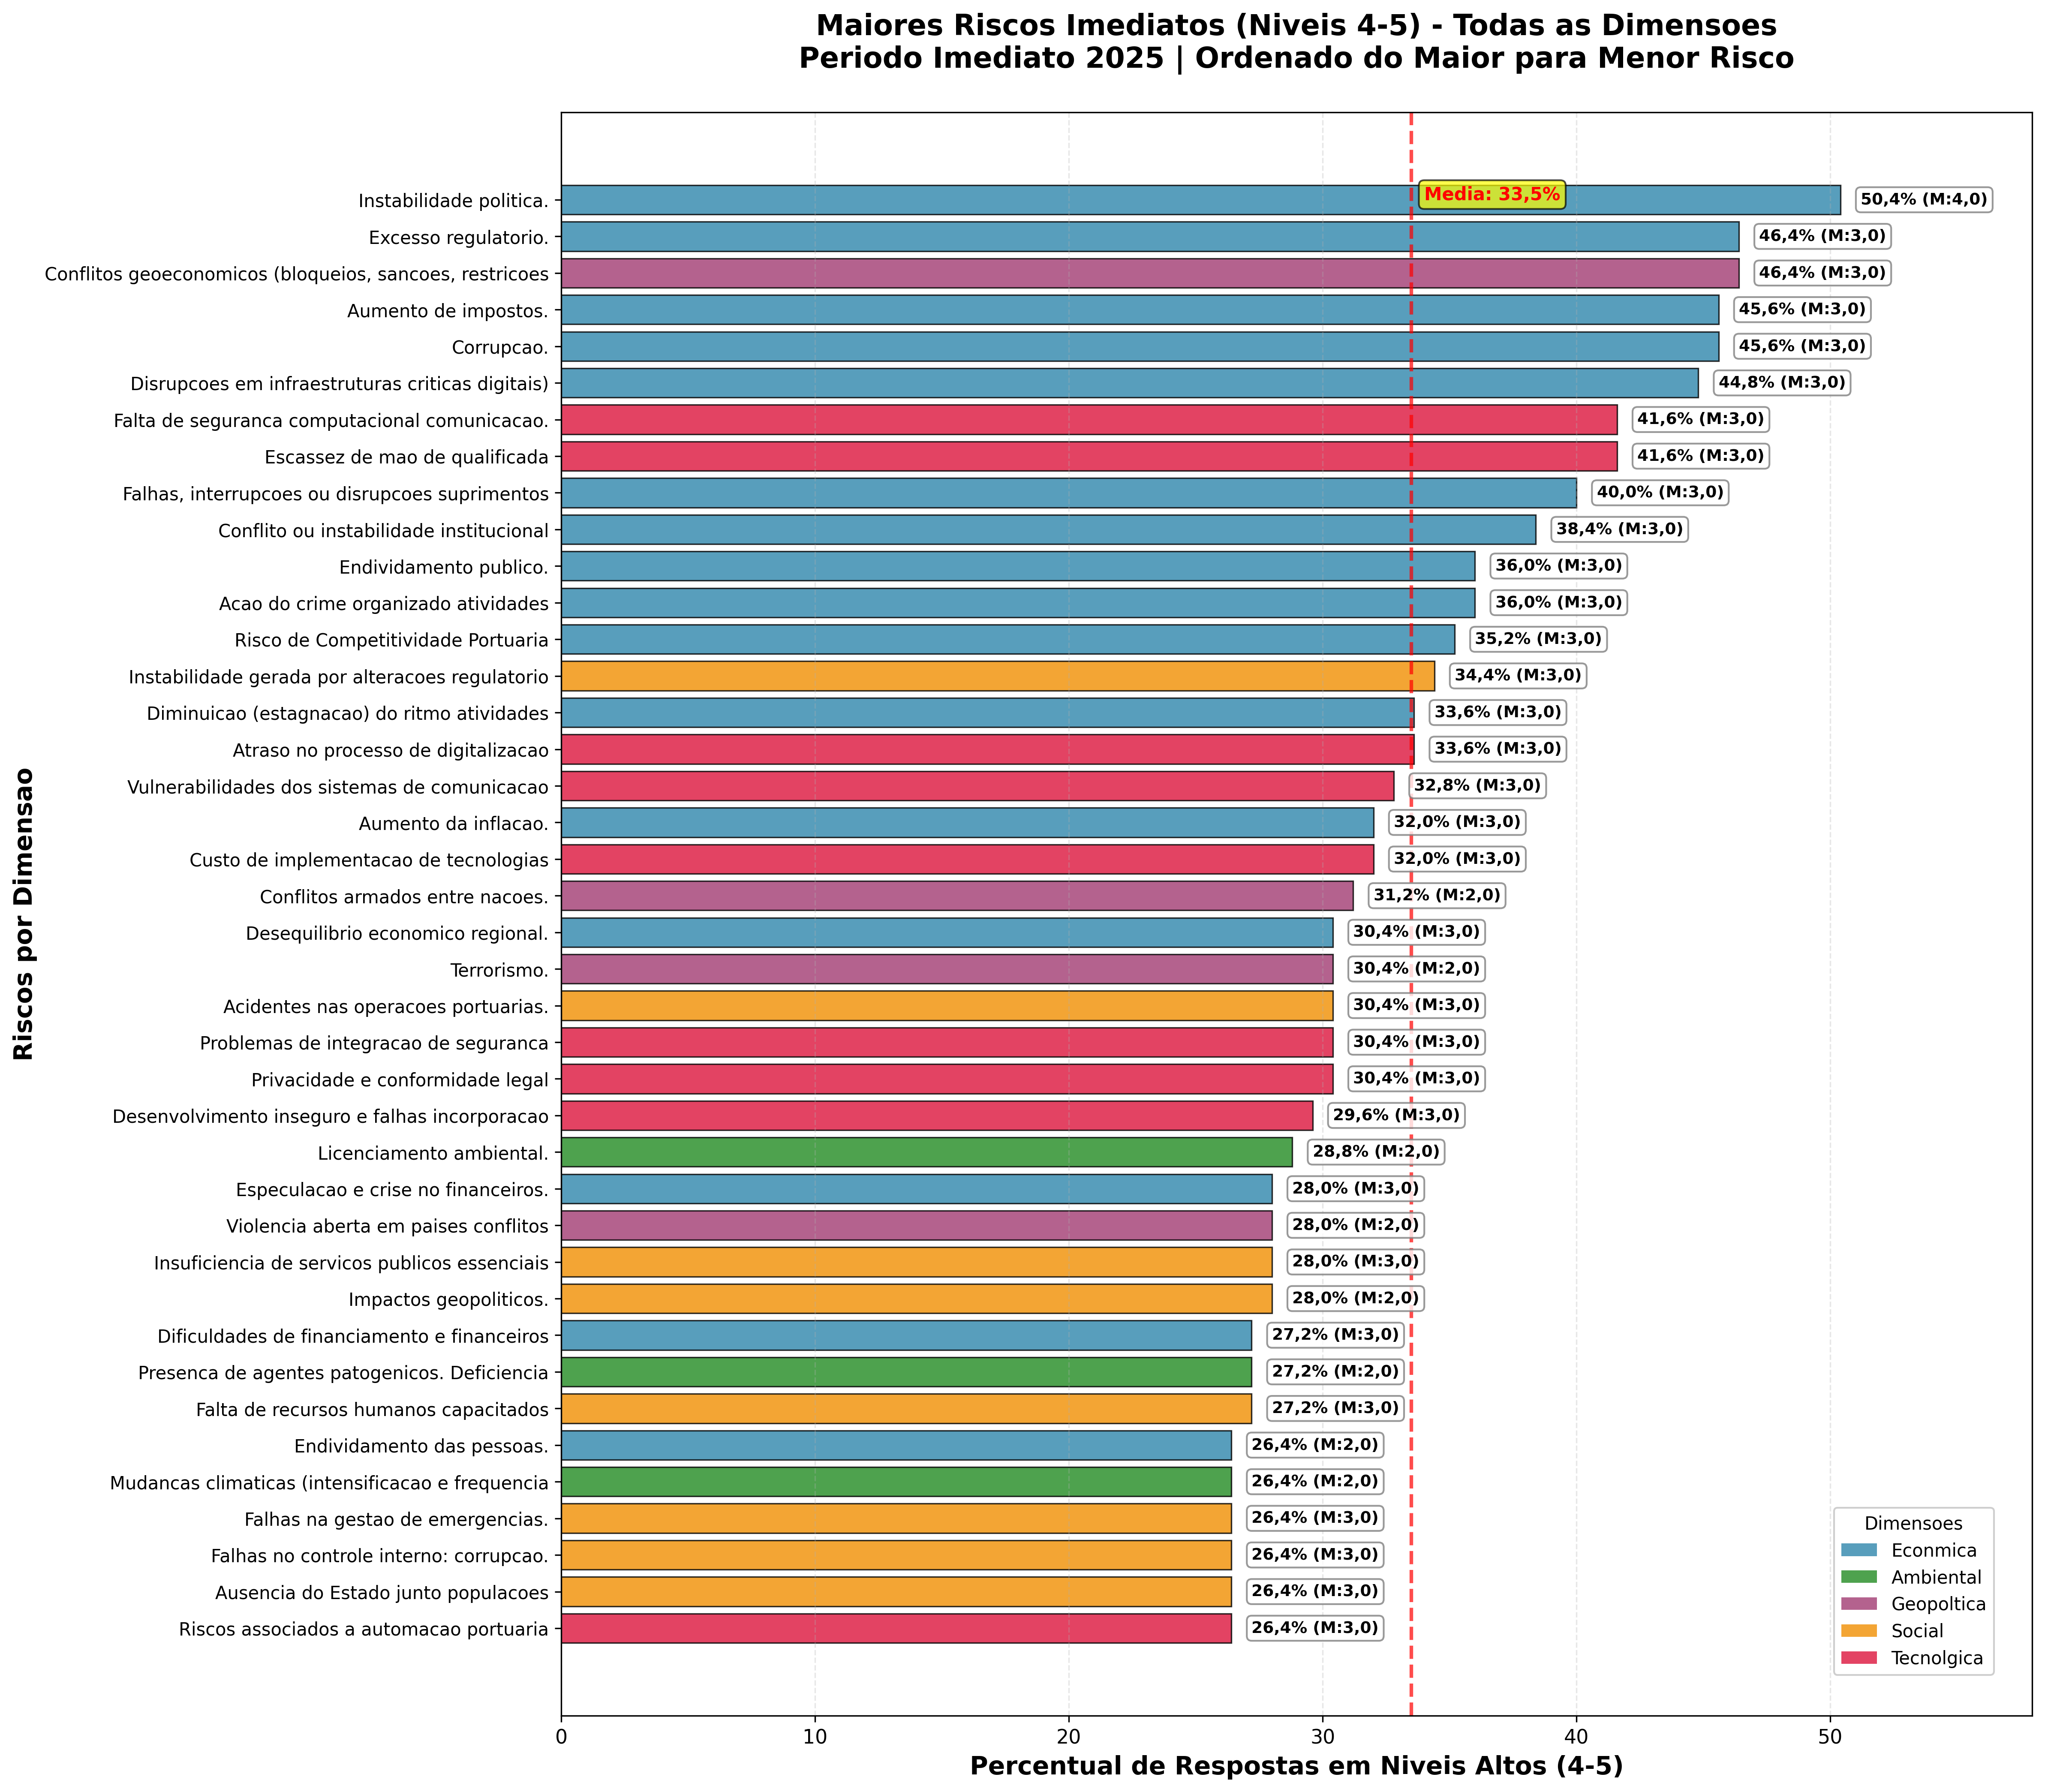
\includegraphics[keepaspectratio]{assets/graficos_agrupados/grafico_interconexao_riscos_imediato_2025.png}}

\subsection{Análise dos Principais
Destaques}\label{anuxe1lise-dos-principais-destaques}

\begin{tcolorbox}[enhanced jigsaw, titlerule=0mm, colback=white, title=\textcolor{quarto-callout-important-color}{\faExclamation}\hspace{0.5em}{Riscos Críticos Identificados}, opacityback=0, colbacktitle=quarto-callout-important-color!10!white, leftrule=.75mm, left=2mm, colframe=quarto-callout-important-color-frame, bottomrule=.15mm, bottomtitle=1mm, breakable, toprule=.15mm, toptitle=1mm, opacitybacktitle=0.6, arc=.35mm, coltitle=black, rightrule=.15mm]

Foram identificados \textbf{6 riscos críticos} (\textgreater40\% de
percepção em níveis altos), todos concentrados nas dimensões Econômica e
Geopolítica:

\begin{enumerate}
\def\labelenumi{\arabic{enumi}.}
\tightlist
\item
  \textbf{Instabilidade política} (Econômica): 50\%;
\item
  \textbf{Excesso regulatório} (Econômica): 46\%;
\item
  \textbf{Conflitos geoeconômicos} (Geopolítica): 46\%;
\item
  \textbf{Aumento de impostos} (Econômica): 46\%;
\item
  \textbf{Corrupção} (Econômica): 46\%;
\item
  \textbf{Disrupções em infraestruturas críticas digitais} (Econômica):
  45\%.
\end{enumerate}

\end{tcolorbox}

\subsection{Padrões por Dimensão}\label{padruxf5es-por-dimensuxe3o}

\begin{itemize}
\tightlist
\item
  \textbf{Dimensão Econômica}: Apresenta a maior concentração de riscos
  críticos, com 13 dos 20 riscos analisados e média de 39\% de percepção
  de risco alto.
\item
  \textbf{Dimensão Geopolítica}: Embora com menor quantidade de riscos,
  apresenta níveis elevados, especialmente em conflitos geoeconômicos.
\item
  \textbf{Dimensões Social, Ambiental e Tecnológica}: Apresentam riscos
  mais moderados, mas ainda relevantes para gestão integrada.
\end{itemize}

O gr?fico a seguir apresenta a dispers?o temporal das vari?veis,
comparando curto e longo prazo.
\pandocbounded{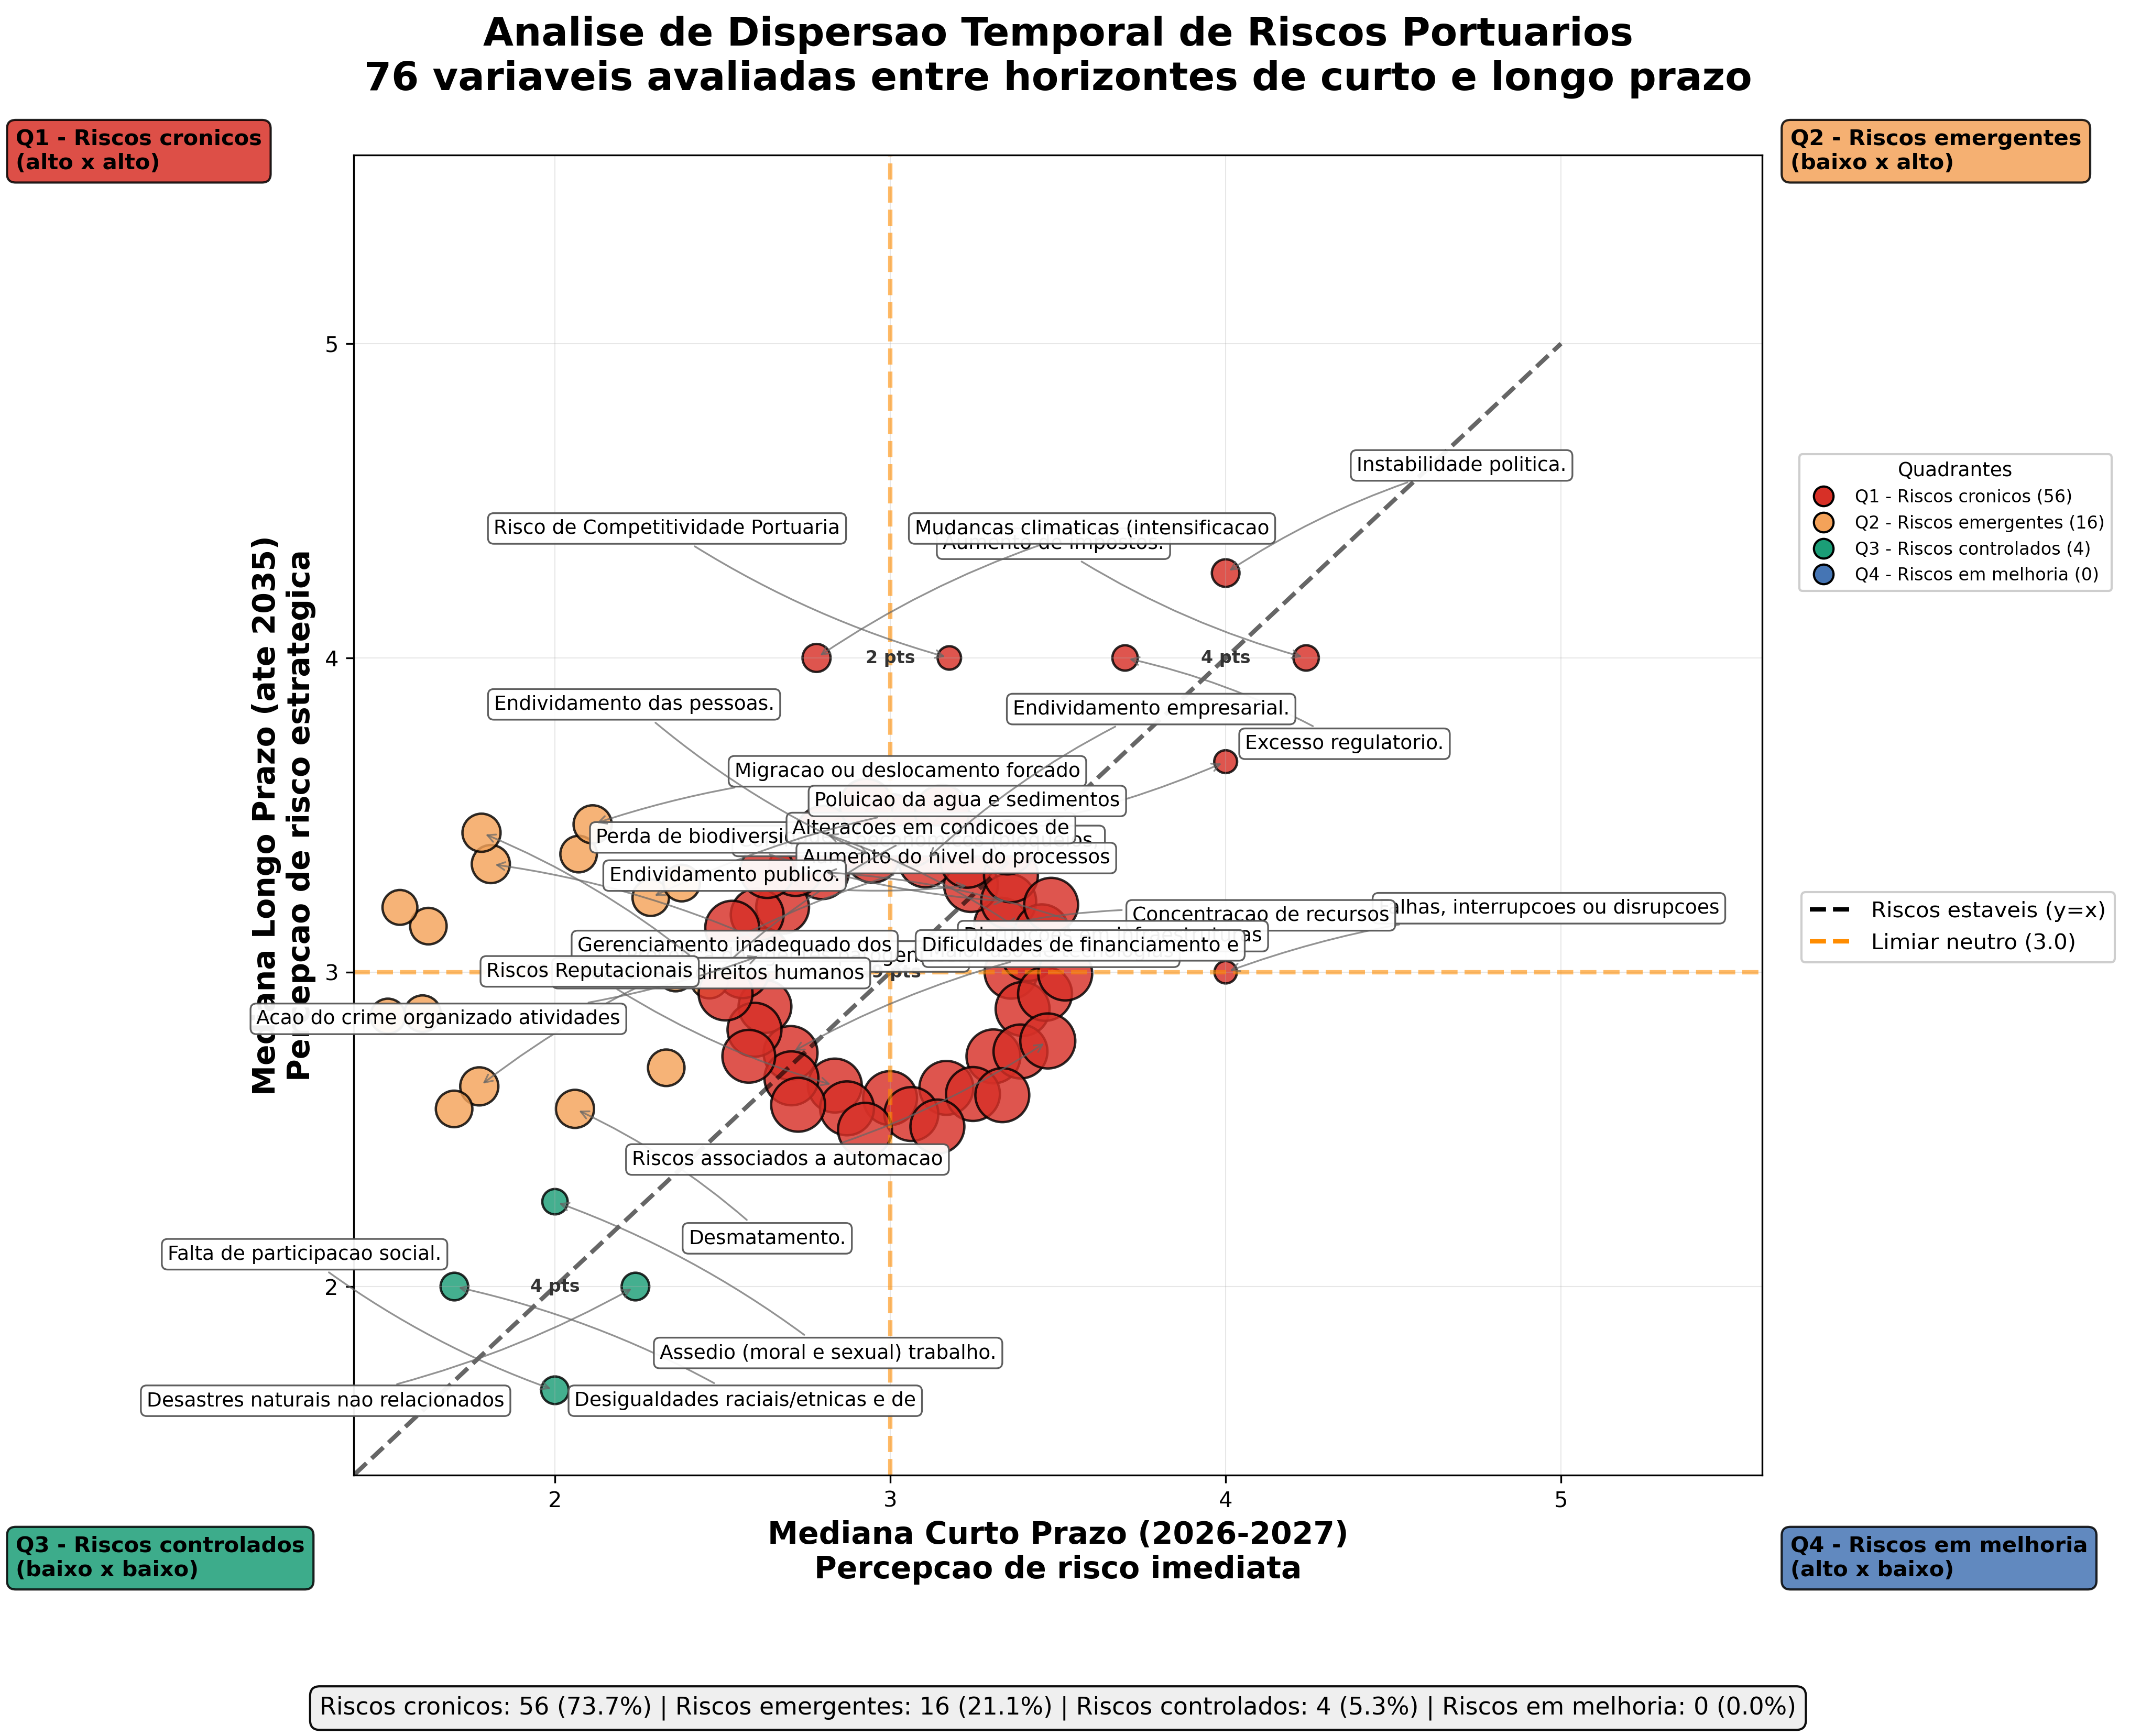
\includegraphics[keepaspectratio]{assets/graficos_agrupados/grafico_dispersao_temporal_riscos_ampliado.png}}

\subsection{Principais Achados da Análise de
Dispersão}\label{principais-achados-da-anuxe1lise-de-dispersuxe3o}

O gráfico de dispersão temporal revela padrões importantes na evolução
dos riscos entre o curto prazo (2026-2027) e longo prazo (até 2035):

\subsubsection{Correlação e Persistência dos
Riscos}\label{correlauxe7uxe3o-e-persistuxeancia-dos-riscos}

\begin{itemize}
\item
  \textbf{Correlação moderada (r = 0,639)}: Indica que a hierarquia de
  riscos tende a se manter, mas com mudanças significativas em casos
  específicos;- \textbf{Delta médio de +0,19 ponto}: Sugere uma leve
  piora geral dos riscos ao longo do tempo;- \textbf{74\% dos riscos são
  crônicos}: Permanecem em níveis elevados em ambos os horizontes
  temporais. \#\#\#\# Análise por Quadrantes
\item
  \textbf{Quadrante 1 - Riscos Crônicos (alto x alto)}: 42 variáveis,
  principalmente econômicas e geopolíticas;- \textbf{Quadrante 2 -
  Riscos Emergentes (baixo x alto)}: 11 variáveis, predominantemente
  ambientais;- \textbf{Quadrante 3 - Riscos Controlados (baixo x
  baixo)}: 4 variáveis, mantidas sob controle;- \textbf{Quadrante 4 -
  Riscos em Melhoria (alto x baixo)}: Nenhuma variável, indicando
  ausência de melhorias consistentes. \#\#\#\# Insights por Dimensão
\item
  \textbf{Ambiental}: Maior piora temporal (delta +0,56), com 5
  variáveis aumentando +1.0 ponto;- \textbf{Econômica}: Relativa
  estabilidade (delta -0,05), com riscos mantidos em níveis elevados;-
  \textbf{Geopolítica}: Piora moderada (delta +0,40), especialmente em
  riscos de contaminação;- \textbf{Social}: Variação leve (delta +0,08),
  com preocupações consistentes sobre direitos humanos;-
  \textbf{Tecnológica}: Estabilidade completa (delta 0,00), indicando
  percepção constante dos riscos digitais. \#\#\#\# Implicações
  Estratégicas
\end{itemize}

A ausência de riscos em melhoria (Quadrante 4 vazio) e a predominância
de riscos crônicos destacam a necessidade de ações preventivas e
mitigatórias contínuas, especialmente para os desafios ambientais que
mostram o maior agravamento temporal.

\section{Evolução Temporal}\label{evoluuxe7uxe3o-temporal}

O gráfico de dispersão temporal apresenta a evolução temporal completa
das 57 variáveis de risco analisadas, conectando suas medianas entre o
curto prazo (2026-2027) e o longo prazo (até 2035). As cores representam
as dimensões dos riscos e a transparência das linhas indica a magnitude
da mudança temporal.

O gr?fico a seguir resume a evolu??o temporal das vari?veis de risco
entre curto e longo prazo.
\pandocbounded{\includegraphics[keepaspectratio]{assets/graficos_agrupados/slopegraph_centro_conectores_cor_unica.png}}

\subsection{Insights}\label{insights}

\subsubsection{Distribuição das Mudanças por
Dimensão}\label{distribuiuxe7uxe3o-das-mudanuxe7as-por-dimensuxe3o}

\begin{itemize}
\tightlist
\item
  \textbf{Ambiental (16 variáveis)}: Maior piora temporal, com delta
  médio de +0,56;- \textbf{Econômica (19 variáveis)}: Única dimensão com
  melhoria média (-0,05);- \textbf{Geopolítica (5 variáveis)}: Piora
  moderada, com delta médio de +0,40;- \textbf{Social (13 variáveis)}:
  Piora leve, com delta médio de +0,08;- \textbf{Tecnológica (4
  variáveis)}: Estável, com delta médio de 0,00. \#\#\#\# Principais
  Padrões Identificados
\end{itemize}

\textbf{Pioras Críticas (+1.0 ponto) - 11 variáveis:}

\begin{itemize}
\item
  \textbf{Ambiental (9 variáveis)}: Mudanças climáticas, aumento do
  nível do mar, poluição, espécies exóticas, resíduos, desmatamento,
  ruídos, patógenos, produtos perigosos;
\item
  \textbf{Geopolítica (2 variáveis)}: Terrorismo, liberação de agentes
  biológicos;
\item
  \textbf{Social (1 variável)}: Ameaças aos direitos humanos.
  \textbf{Melhoria Significativa (-1.0 ponto) - 1 variável:}
\item
  \textbf{Econômica}: Falhas, interrupções ou disrupções em
  infraestruturas críticas digitais. \textbf{Estabilidade em Níveis
  Elevados (44 variáveis):}
\item
  Predominância de riscos econômicos mantidos em mediana 3.0-4.0;-
  Riscos tecnológicos completamente estáveis em mediana 3.0;- Riscos
  sociais e geopolíticos com variações mínimas. \#\#\#\# Análise
  Estatística Geral (Variáveis com Mediana ≥ 3.0)
\item
  \textbf{Total analisado}: 42 variáveis (74\% do total);- \textbf{Delta
  médio geral}: 0,000 (equilíbrio geral);- \textbf{Desvio padrão}: 0,218
  (baixa variabilidade);- \textbf{Variáveis com piora}: 1 (2\%);-
  \textbf{Variáveis com melhoria}: 1 (2\%);- \textbf{Variáveis
  estáveis}: 40 (95\%). \#\#\#\# Padrões Específicos Identificados
\end{itemize}

\textbf{Mudança Significativa de Melhoria:}

\begin{itemize}
\item
  \textbf{Falhas em infraestruturas críticas digitais} (Econômica): 4.00
  → 3.00 (-1.00). \textbf{Mudança Significativa de Piora:}
\item
  \textbf{Mudanças climáticas} (Ambiental): 3.00 → 4.00 (+1.00).
  \textbf{Estabilidade Generalizada:}
\item
  \textbf{40 variáveis} permaneceram inalteradas, indicando percepção
  consolidada de risco;- \textbf{Econômica}: 19 variáveis estáveis em
  níveis elevados (3.0-4.0);- \textbf{Social e Tecnológica}: Todas as
  variáveis completamente estáveis em mediana 3.0;-
  \textbf{Geopolítica}: 3 variáveis estáveis em mediana 3.33. \#\#\#\#
  Implicações Estratégicas
\end{itemize}

Os dados revelam um cenário de alta estabilidade percebida: 95\% das
variáveis com risco elevado mantiveram-se inalteradas entre os
horizontes temporais. Este padrão sugere:

\begin{enumerate}
\def\labelenumi{\arabic{enumi}.}
\tightlist
\item
  \textbf{Consolidação da Percepção de Risco}: Os stakeholders possuem
  visões bem estabelecidas sobre os riscos portuários;2. \textbf{Foco em
  Dois Pontos Críticos}: Apenas duas variáveis mostraram mudança
  significativa, permitindo ação focada;3. \textbf{Prioridade para
  Mudanças Climáticas}: Única variável com piora significativa exige
  atenção estratégica;4. \textbf{Oportunidade em Infraestrutura
  Digital}: Melhoria identificada pode ser alavancada como caso de
  sucesso. A estabilidade predominante indica, na percepção dos
  gestores, que as estratégias de gestão de riscos atuais são adequadas
  para manter os níveis de risco, mas insuficientes para reduzi-los
  significativamente.
\end{enumerate}

\bookmarksetup{startatroot}

\chapter{Riscos Econômicos}\label{riscos-econuxf4micos-1}

Este capítulo apresenta a análise dos riscos econômicos identificados
organizados por horizontes temporais e aspectos específicos.

\section{Visão Geral dos Riscos
Econômicos}\label{visuxe3o-geral-dos-riscos-econuxf4micos}

Os riscos econômicos foram avaliados em três horizontes temporais:

\begin{itemize}
\tightlist
\item
  \textbf{Imediato (2025)}: Riscos que requerem atenção imediata;-
  \textbf{Curto Prazo (2026-2027)}: Riscos emergentes que demandam
  planejamento;- \textbf{Longo Prazo (até 2035)}: Riscos estratégicos
  que requerem visão de futuro. \#\# Panorama do Período Imediato
\end{itemize}

O gr?fico a seguir mostra a distribui??o dos riscos no per?odo imediato.
\pandocbounded{\includegraphics[keepaspectratio]{assets/economicos/grafico_barras_imediato_2025.png}}

\begin{tcolorbox}[enhanced jigsaw, titlerule=0mm, colback=white, title=\textcolor{quarto-callout-note-color}{\faInfo}\hspace{0.5em}{Destaques do período Imediato de 2025}, opacityback=0, colbacktitle=quarto-callout-note-color!10!white, leftrule=.75mm, left=2mm, colframe=quarto-callout-note-color-frame, bottomrule=.15mm, bottomtitle=1mm, breakable, toprule=.15mm, toptitle=1mm, opacitybacktitle=0.6, arc=.35mm, coltitle=black, rightrule=.15mm]

\begin{itemize}
\tightlist
\item
  \textbf{Instabilidade política}: 50\% das respostas em níveis altos
  (4-5);
\item
  \textbf{Excesso regulatório}: 46\% em níveis altos;
\item
  \textbf{Aumento de impostos}: 46\% em níveis altos.
\end{itemize}

\end{tcolorbox}

\section{Análise Temporal da Dimensão
Econômica}\label{anuxe1lise-temporal-da-dimensuxe3o-econuxf4mica}

O gr?fico a seguir sintetiza a evolu??o temporal das vari?veis da
dimens?o econ?mica.
\pandocbounded{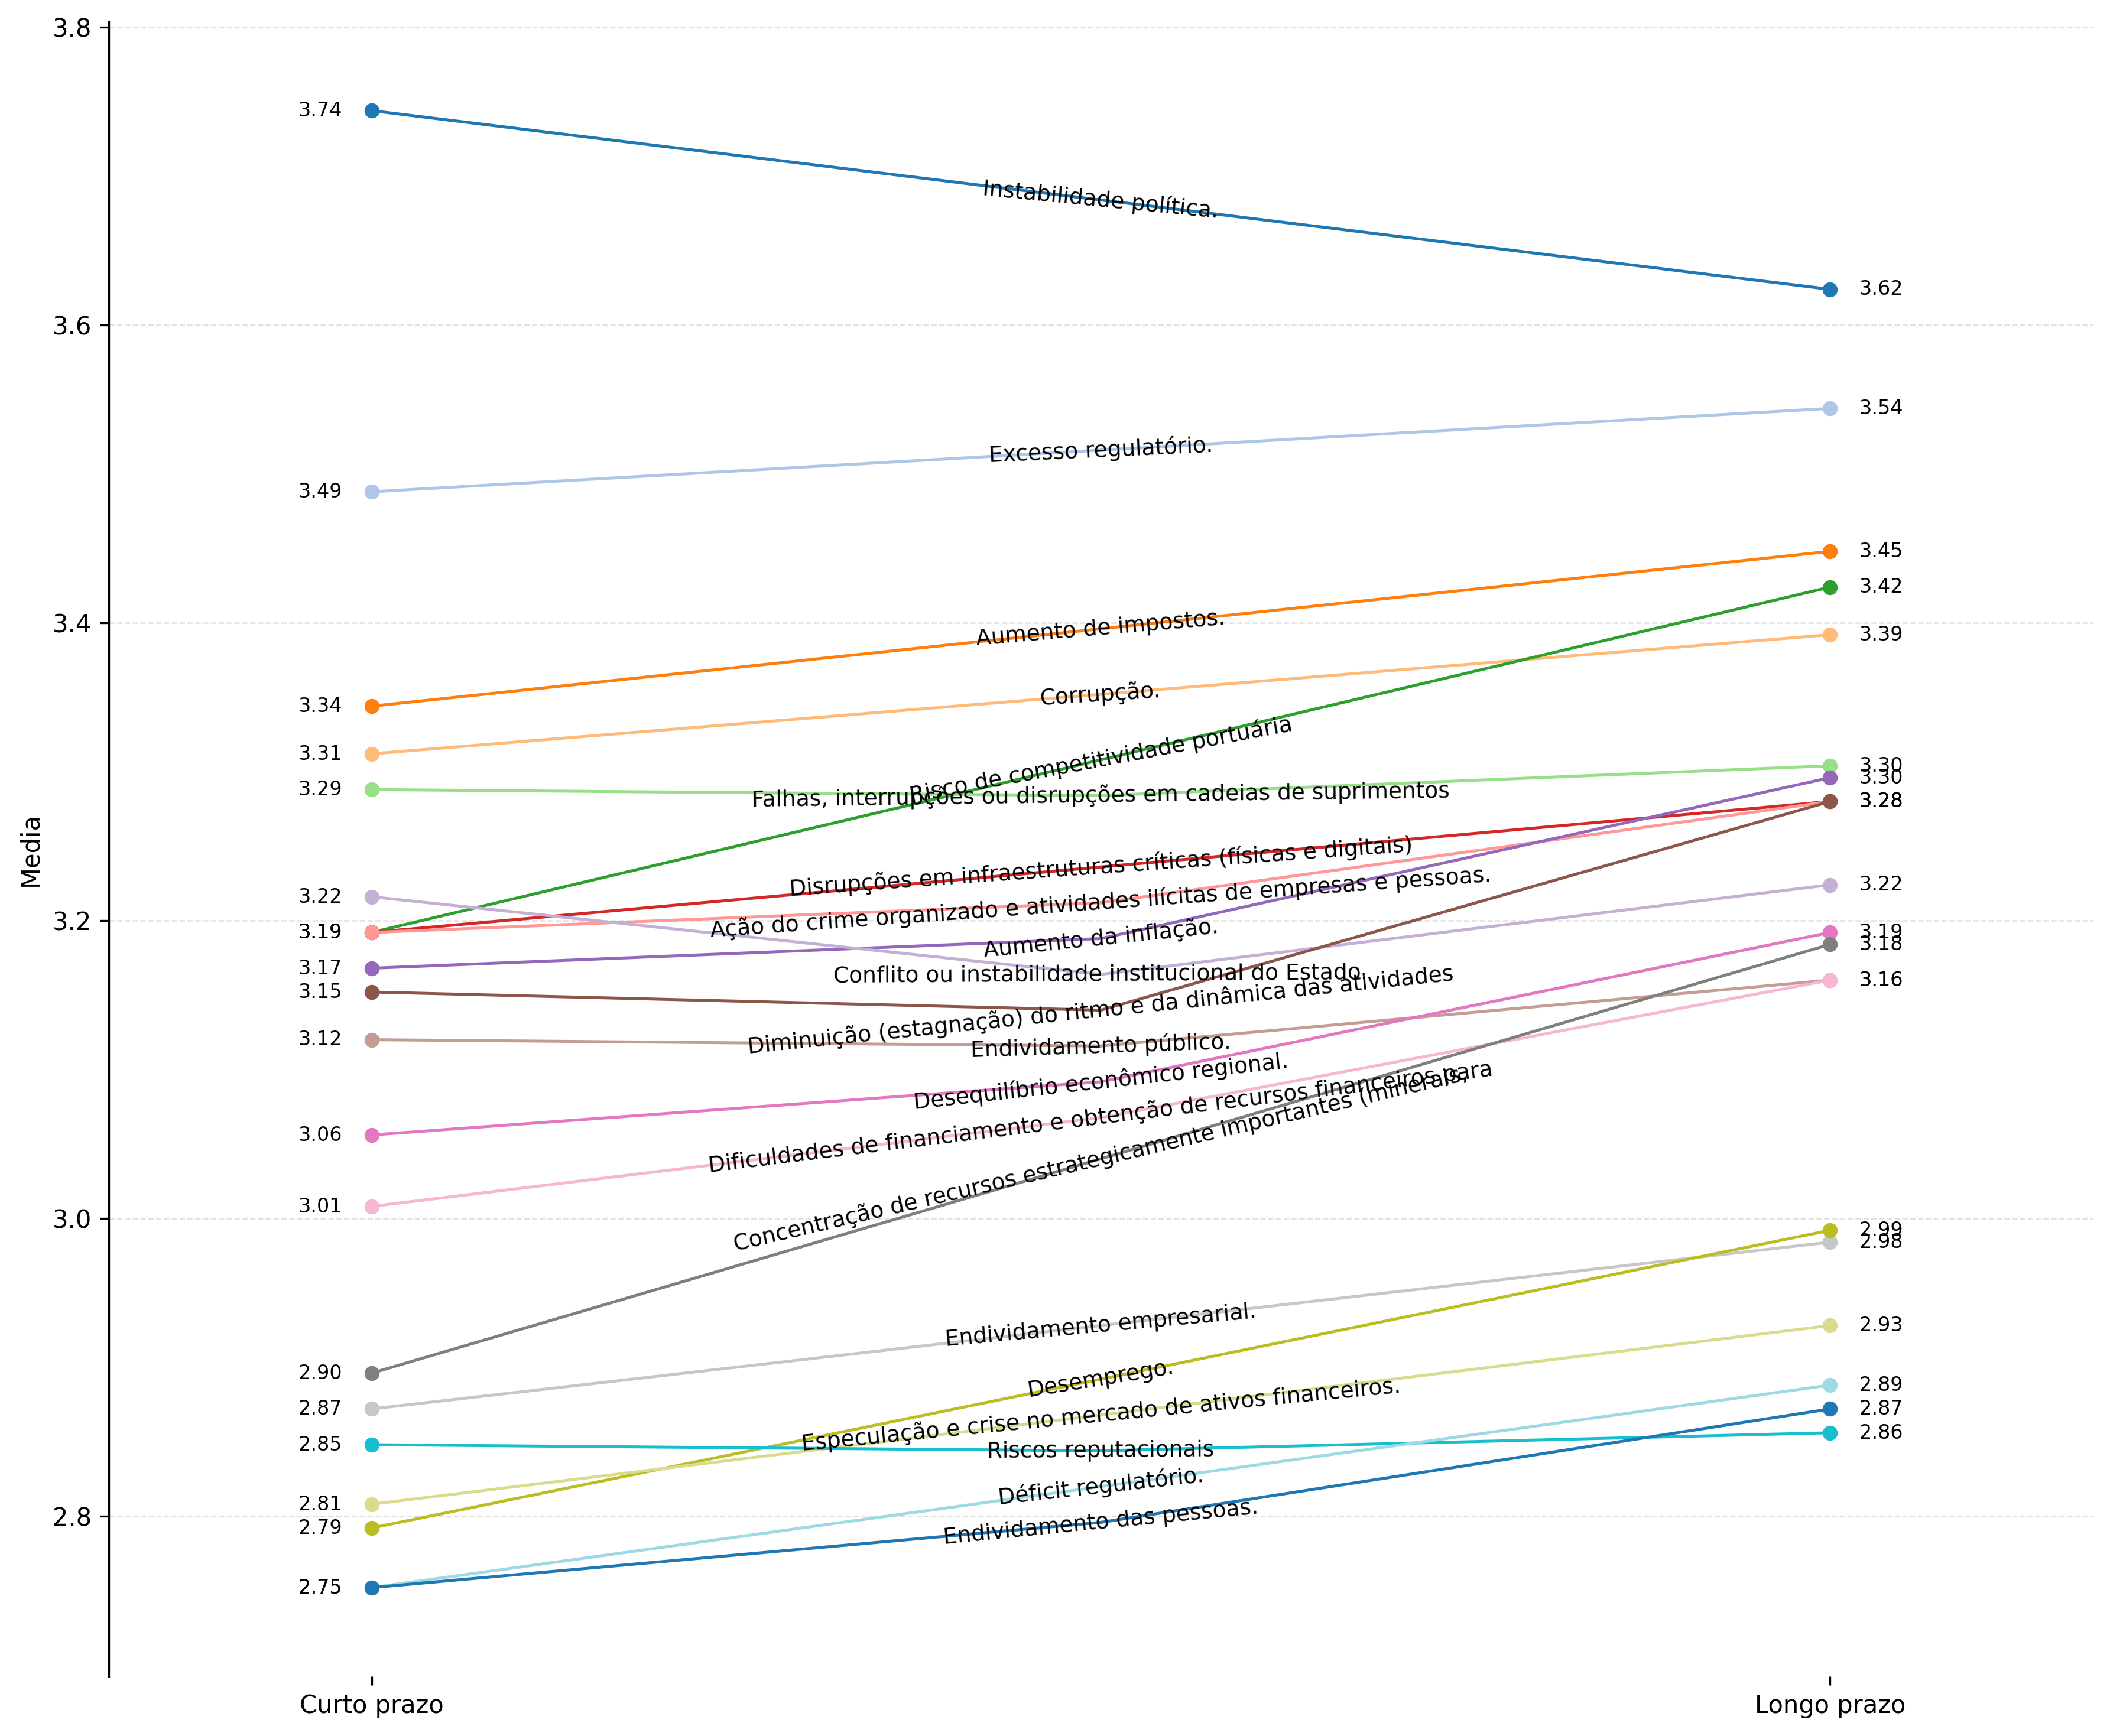
\includegraphics[keepaspectratio]{assets/slopegraphs_por_dimensao/slopegraph_econômica.png}}

A dimensão econômica apresenta 19 variáveis com médias superiores a 2.5
no curto prazo, demonstrando a preocupação significativa com fatores
financeiros e de mercado. Os slopegraphs revelam as trajetórias
individuais de cada risco econômico, permitindo identificar quais
tendências apresentam maior ou menor resiliência temporal.

\subsection{Insights da Análise Temporal
Econômica}\label{insights-da-anuxe1lise-temporal-econuxf4mica}

A análise temporal dos riscos econômicos revela padrões distintos em
comparação com outras dimensões:

\subsubsection{Estabilidade Relativa dos Riscos
Econômicos}\label{estabilidade-relativa-dos-riscos-econuxf4micos}

\begin{itemize}
\item
  \textbf{Delta médio de -0,05}: Única dimensão com melhoria média
  percebida;- \textbf{19 variáveis estáveis}: A maioria dos riscos
  mantém-se constante entre períodos;- \textbf{Ausência de volatilidade
  extrema}: Mudanças limitadas a ±1.0 ponto na maioria dos casos.
  \#\#\#\# Padrões Específicos Identificados
\item
  \textbf{Riscos Crônicos Elevados}: Instabilidade política, excesso
  regulatório e aumento de impostos mantêm-se persistentemente altos;-
  \textbf{Melhoria Significativa}: Falhas em infraestruturas críticas
  digitais apresenta melhoria de -1.0 ponto;- \textbf{Estabilidade em
  Níveis Críticos}: A maioria das variáveis mantém-se em mediana
  3.0-4.0. \#\#\#\# Destaques da Evolução Temporal
\item
  \textbf{Risco Mais Crítico Persistente}: Instabilidade política
  mantém-se como principal preocupação;- \textbf{Pressão Regulatória
  Crescente}: Excesso regulatório e aumento de impostos mostram
  tendência de elevação;- \textbf{Resiliência Operacional}: Riscos
  operacionais mostram maior capacidade de adaptação. \#\#\#\#
  Implicações Estratégicas para a Dimensão Econômica
\end{itemize}

A análise temporal econômica sugere:

1. \textbf{Foco em Governança}: Priorizar estabilidade política e
ambiente regulatório previsível

2. \textbf{Resiliência Digital}: Fortalecer infraestruturas críticas
como área de sucesso

3. \textbf{Gestão de Custos}: Monitorar pressões inflacionárias e
tributárias

4. \textbf{Diversificação}: Reduzir dependência de mercados e clientes
específicos

\section{Exame das Variáveis de Risco: Resultados e
Tendências}\label{exame-das-variuxe1veis-de-risco-resultados-e-tenduxeancias}

\subsection{Especulação e crise no mercado de ativos
financeiros}\label{especulauxe7uxe3o-e-crise-no-mercado-de-ativos-financeiros}

O gr?fico a seguir apresenta a evolu??o temporal do risco Especulação e
crise no mercado de ativos financeiros.
\pandocbounded{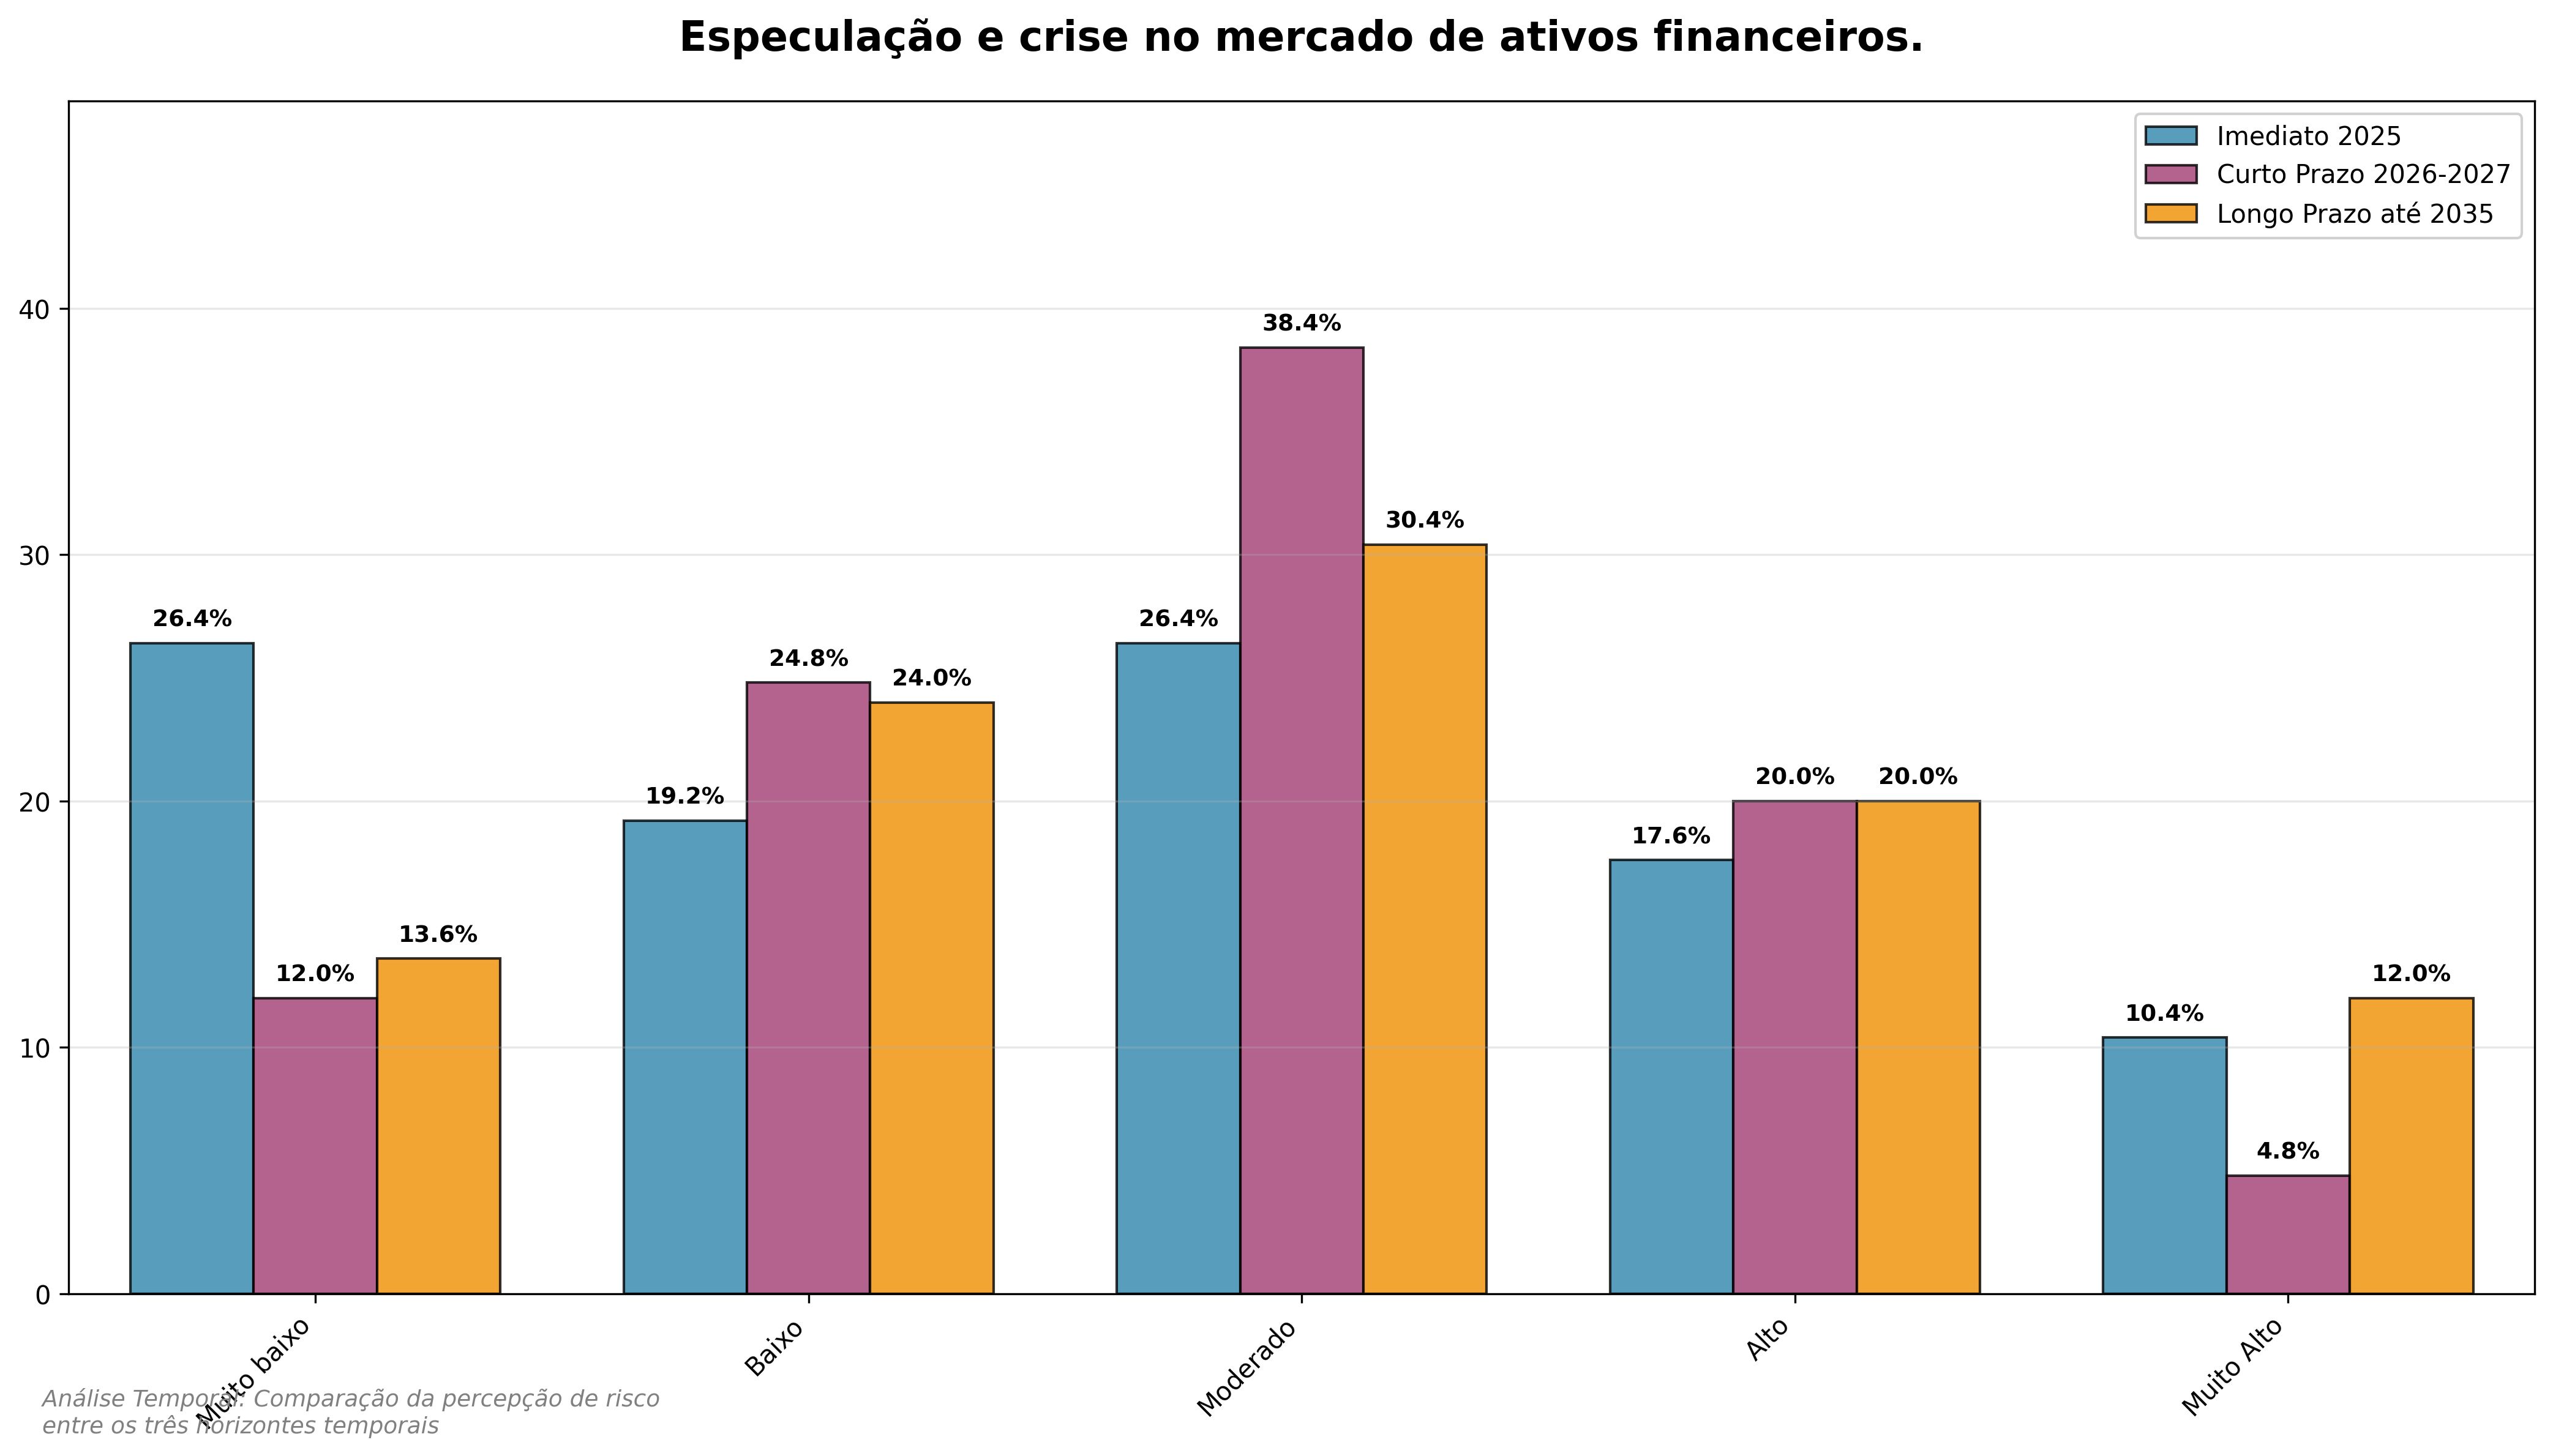
\includegraphics[keepaspectratio]{assets/economicos/grafico_agrupado_1_1_temporal.png}}

\begin{tcolorbox}[enhanced jigsaw, titlerule=0mm, colback=white, title=\textcolor{quarto-callout-tip-color}{\faLightbulb}\hspace{0.5em}{Destaques}, opacityback=0, colbacktitle=quarto-callout-tip-color!10!white, leftrule=.75mm, left=2mm, colframe=quarto-callout-tip-color-frame, bottomrule=.15mm, bottomtitle=1mm, breakable, toprule=.15mm, toptitle=1mm, opacitybacktitle=0.6, arc=.35mm, coltitle=black, rightrule=.15mm]

\textbf{Imediato (2025)}: Mediana 3.0, 28\% em risco alto

\textbf{Curto Prazo (2026-2027)}: Mediana 3.0, 25\% em risco alto

\textbf{Longo Prazo (até 2035)}: Mediana 3.0, 32\% em risco alto

\begin{itemize}
\tightlist
\item
  \textbf{Tendência}: Percepção de risco relativamente estável ao longo
  do tempo. \textbf{Especulação e crise no mercado de ativos
  financeiros. {[}Imediato (2025){]}}
\end{itemize}

Essa percepção de risco é constante no mercado nacional e internacional
de capitais pela volatilidade e facilidade de investimentos em ativos
financeiros. A aversão a esse risco pode conduzir à atenção a
investimentos mais estáveis e controláveis como títulos públicos e menos
a títulos e papéis, eventualmente, com mais rentabilidade, mas mais
incertos e frágeis, às ações especulativas de grandes investidores.

\end{tcolorbox}

\subsection{Concentração de recursos e controle de preços por agentes
econômicos}\label{concentrauxe7uxe3o-de-recursos-e-controle-de-preuxe7os-por-agentes-econuxf4micos}

O gr?fico a seguir apresenta a evolu??o temporal do risco Concentração
de recursos e controle de preços por agentes econômicos.
\pandocbounded{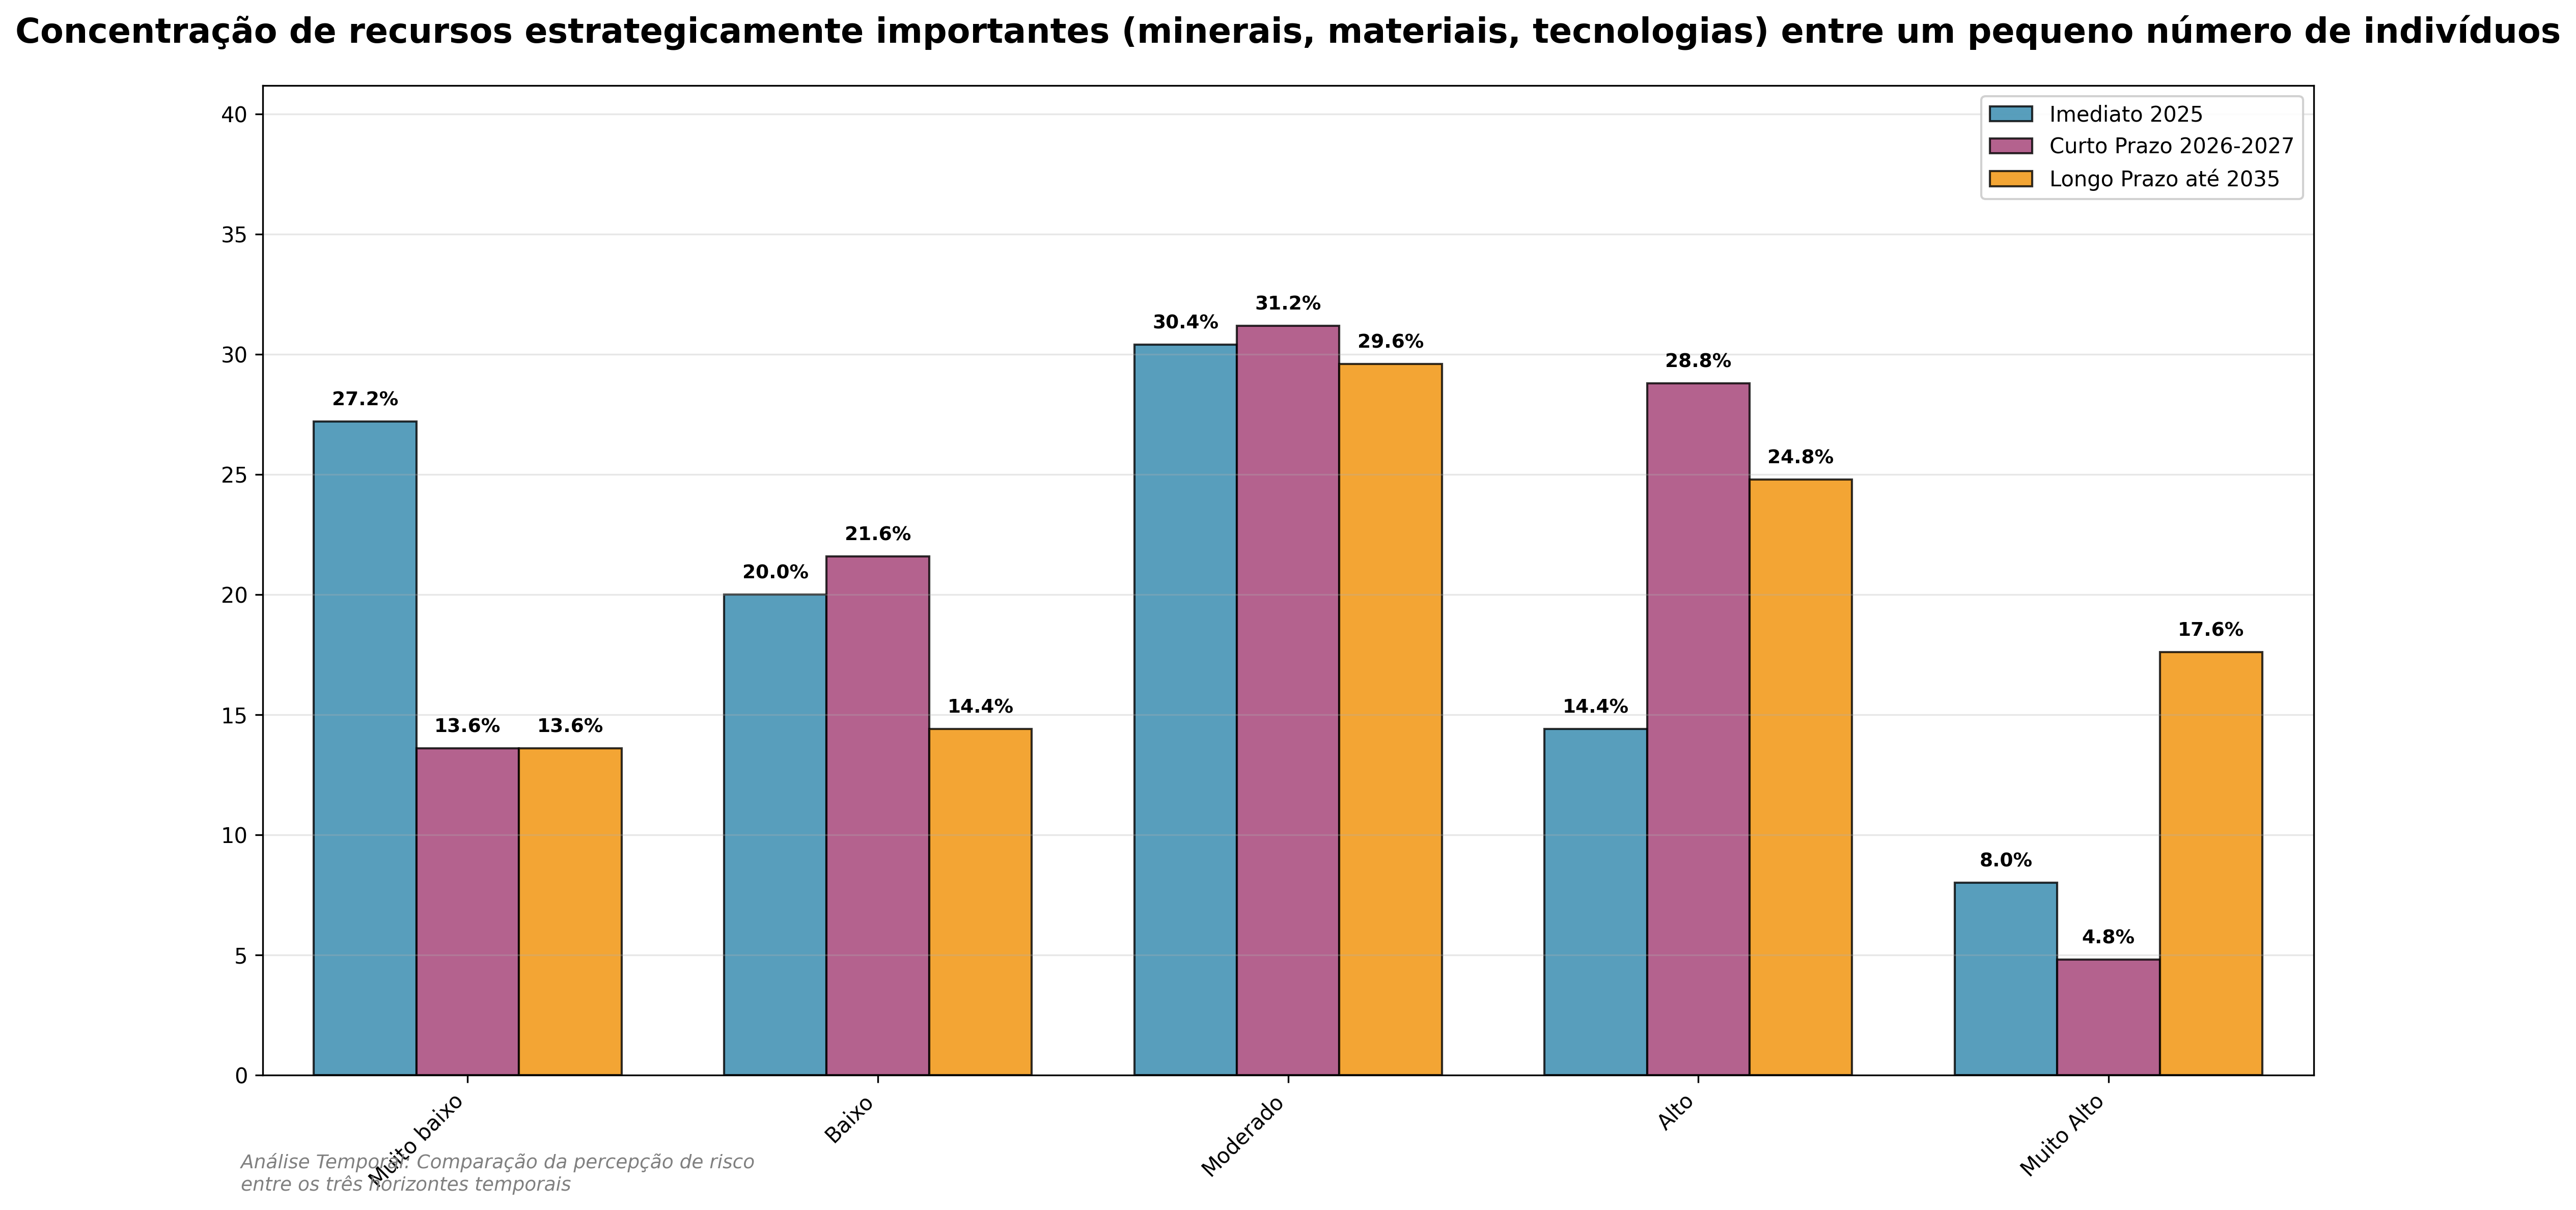
\includegraphics[keepaspectratio]{assets/economicos/grafico_agrupado_1_2_temporal.png}}

\begin{tcolorbox}[enhanced jigsaw, titlerule=0mm, colback=white, title=\textcolor{quarto-callout-tip-color}{\faLightbulb}\hspace{0.5em}{Destaques}, opacityback=0, colbacktitle=quarto-callout-tip-color!10!white, leftrule=.75mm, left=2mm, colframe=quarto-callout-tip-color-frame, bottomrule=.15mm, bottomtitle=1mm, breakable, toprule=.15mm, toptitle=1mm, opacitybacktitle=0.6, arc=.35mm, coltitle=black, rightrule=.15mm]

\textbf{Imediato (2025)}: Mediana 3.0, 22\% em risco alto

\textbf{Curto Prazo (2026-2027)}: Mediana 3.0, 34\% em risco alto

\textbf{Longo Prazo (até 2035)}: Mediana 3.0, 42\% em risco alto

\begin{itemize}
\tightlist
\item
  \textbf{Tendência}: Percepção de risco relativamente estável ao longo
  do tempo. \textbf{Concentração de recursos estrategicamente
  importantes (minerais, materiais, tecnologias) entre um pequeno número
  de indivíduos, empresas ou Estados que podem controlar o acesso e
  ditar preços discricionários. {[}Imediato (2025){]}}
\end{itemize}

Esta condição tem se acentuado com a concentração de propriedades e
acesso a recursos materiais e tecnológicos, que se apresentam no mercado
nacional e internacional. A estrutura concentradora desses mercados
impacta na atividade portuária para lidar com agentes com poder de
negociação e viabilização de parcerias em terminais dedicados.

\end{tcolorbox}

\subsection{Endividamento Público}\label{endividamento-puxfablico}

O gr?fico a seguir apresenta a evolu??o temporal do risco Endividamento
Público.
\pandocbounded{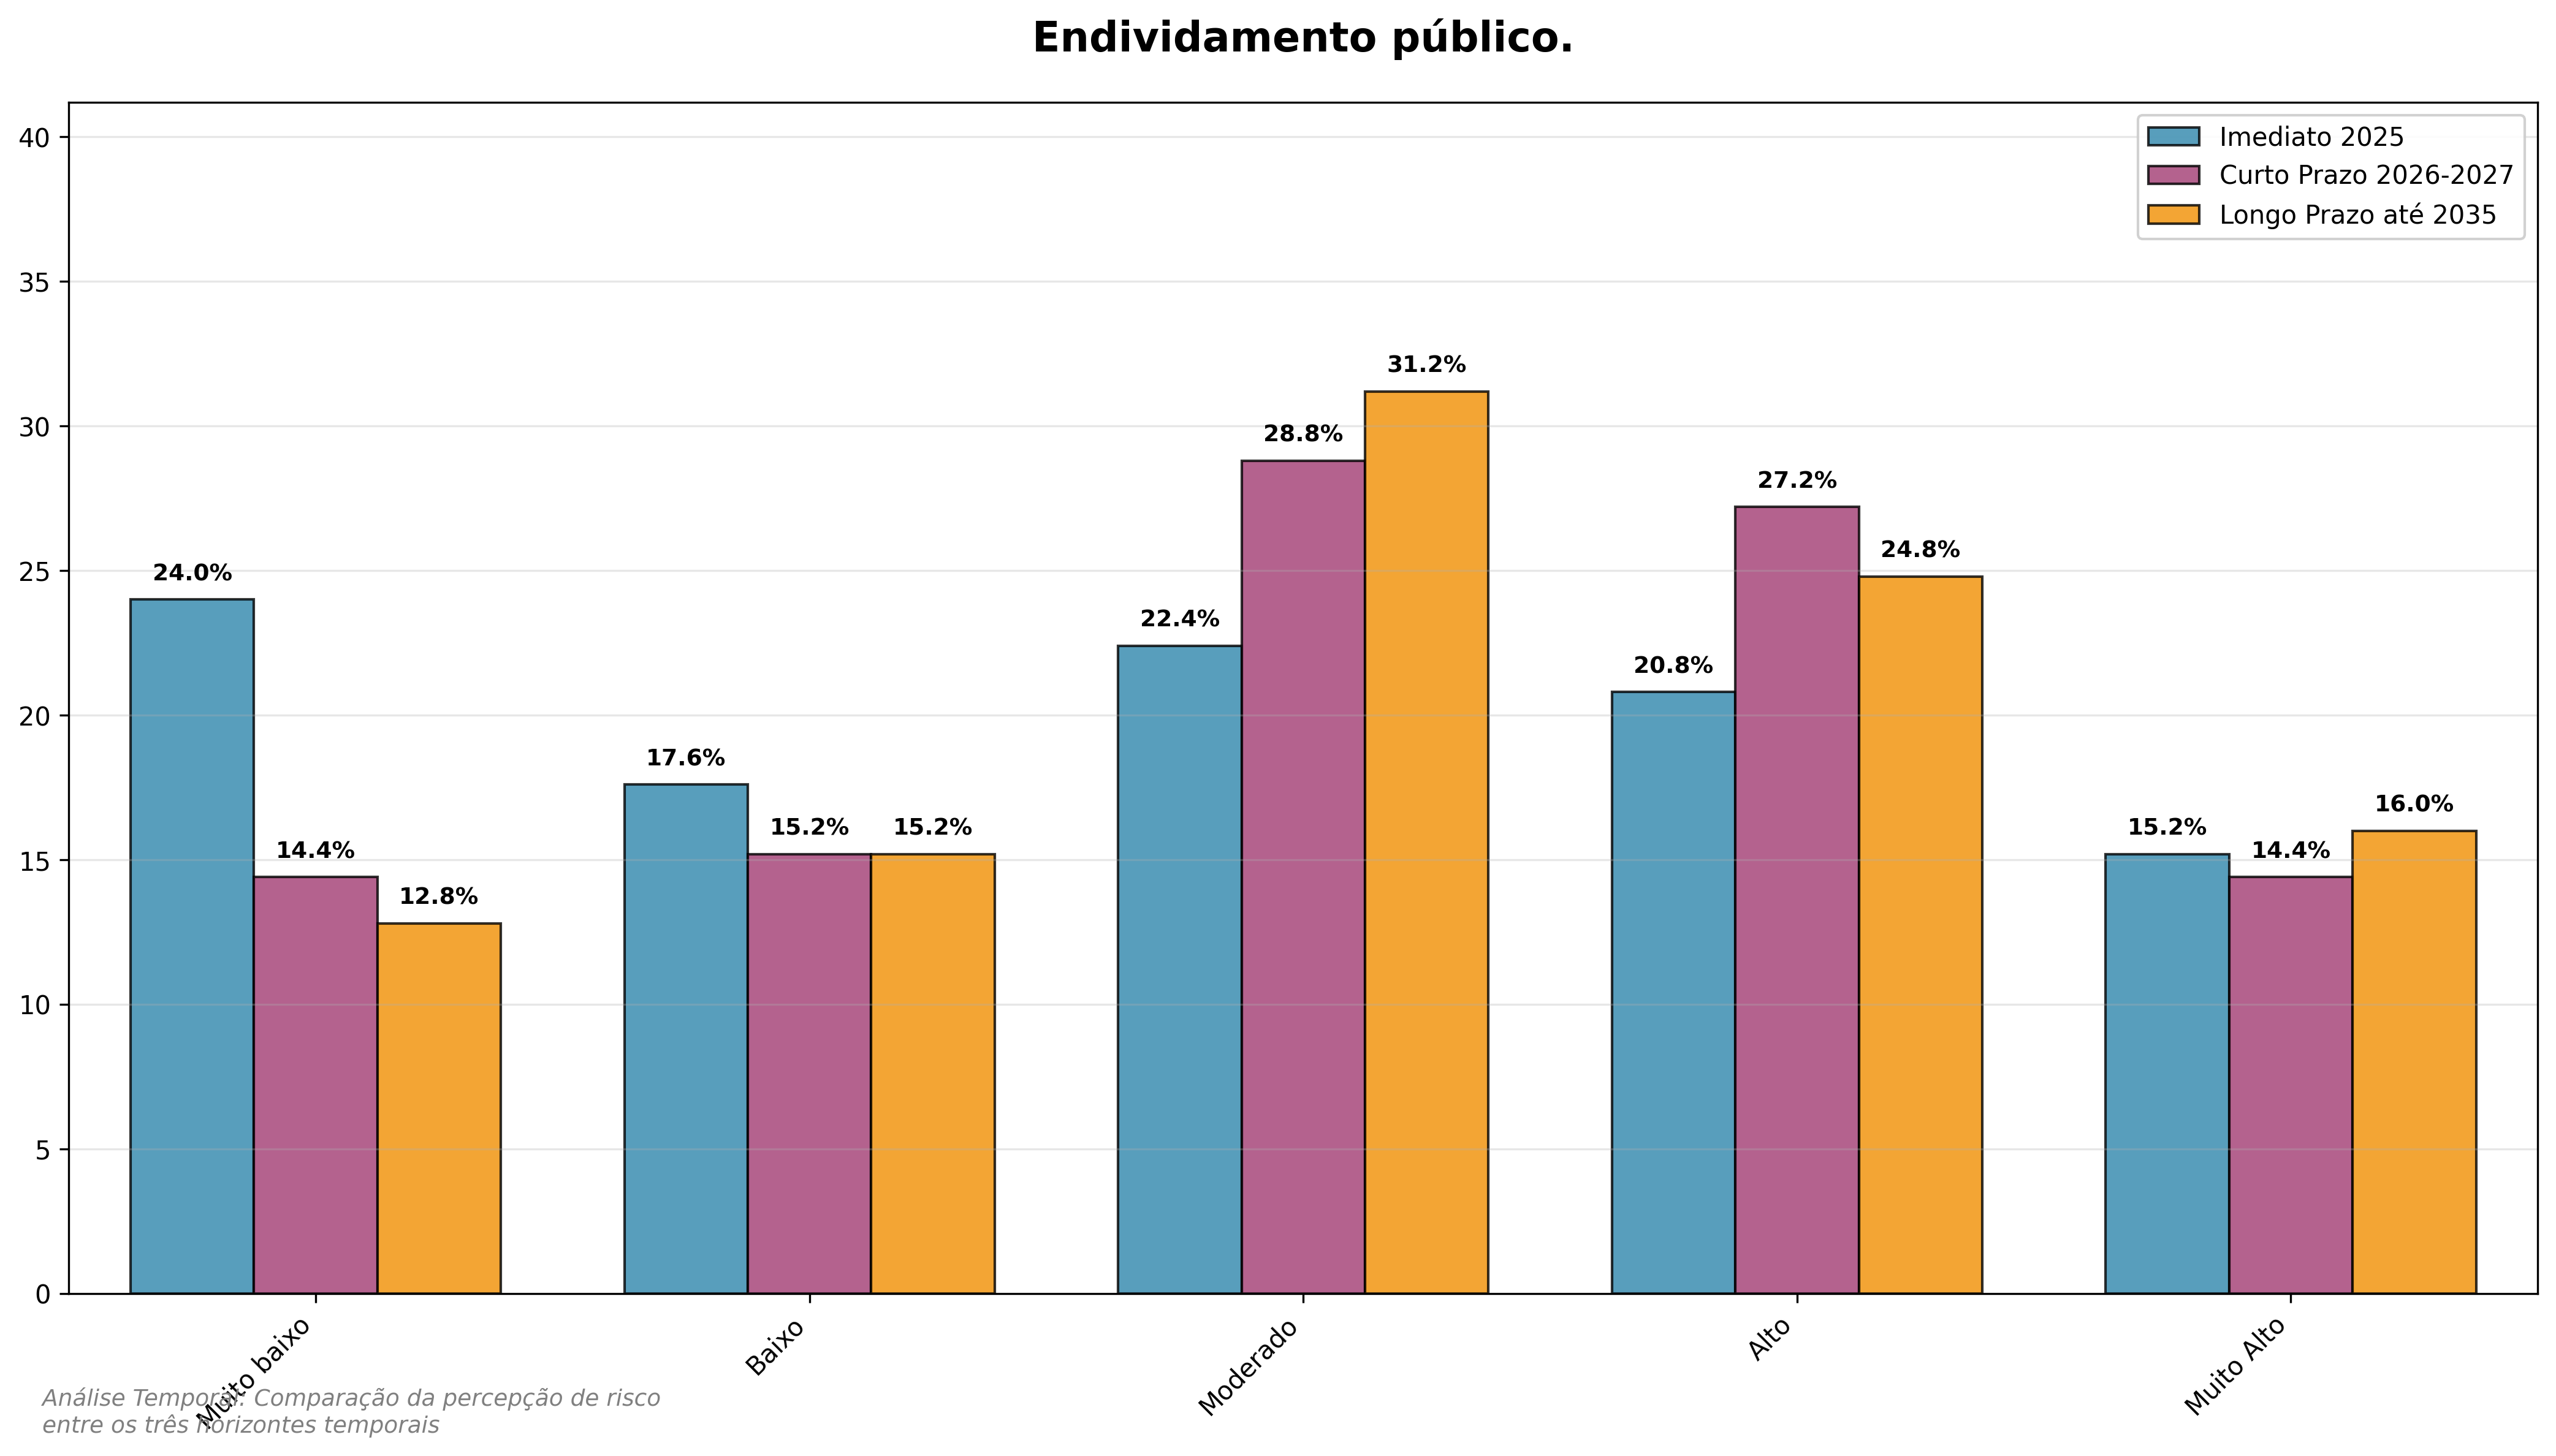
\includegraphics[keepaspectratio]{assets/economicos/grafico_agrupado_1_3_temporal.png}}

\begin{tcolorbox}[enhanced jigsaw, titlerule=0mm, colback=white, title=\textcolor{quarto-callout-tip-color}{\faLightbulb}\hspace{0.5em}{Destaques}, opacityback=0, colbacktitle=quarto-callout-tip-color!10!white, leftrule=.75mm, left=2mm, colframe=quarto-callout-tip-color-frame, bottomrule=.15mm, bottomtitle=1mm, breakable, toprule=.15mm, toptitle=1mm, opacitybacktitle=0.6, arc=.35mm, coltitle=black, rightrule=.15mm]

\textbf{Imediato (2025)}: Mediana 3.0, 36\% em risco alto

\textbf{Curto Prazo (2026-2027)}: Mediana 3.0, 42\% em risco alto

\textbf{Longo Prazo (até 2035)}: Mediana 3.0, 41\% em risco alto

\begin{itemize}
\tightlist
\item
  \textbf{Tendência}: Percepção de risco relativamente estável ao longo
  do tempo. \textbf{Endividamento público. {[}Imediato (2025){]}}
\end{itemize}

Risco devido a eventual impossibilidade ou dificuldade para aportes
públicos ou garantias de empréstimos, principalmente com as altas taxas
de juros que o país tem convivido.

\end{tcolorbox}

\subsection{Endividamento Empresarial}\label{endividamento-empresarial}

O gr?fico a seguir apresenta a evolu??o temporal do risco Endividamento
Empresarial.
\pandocbounded{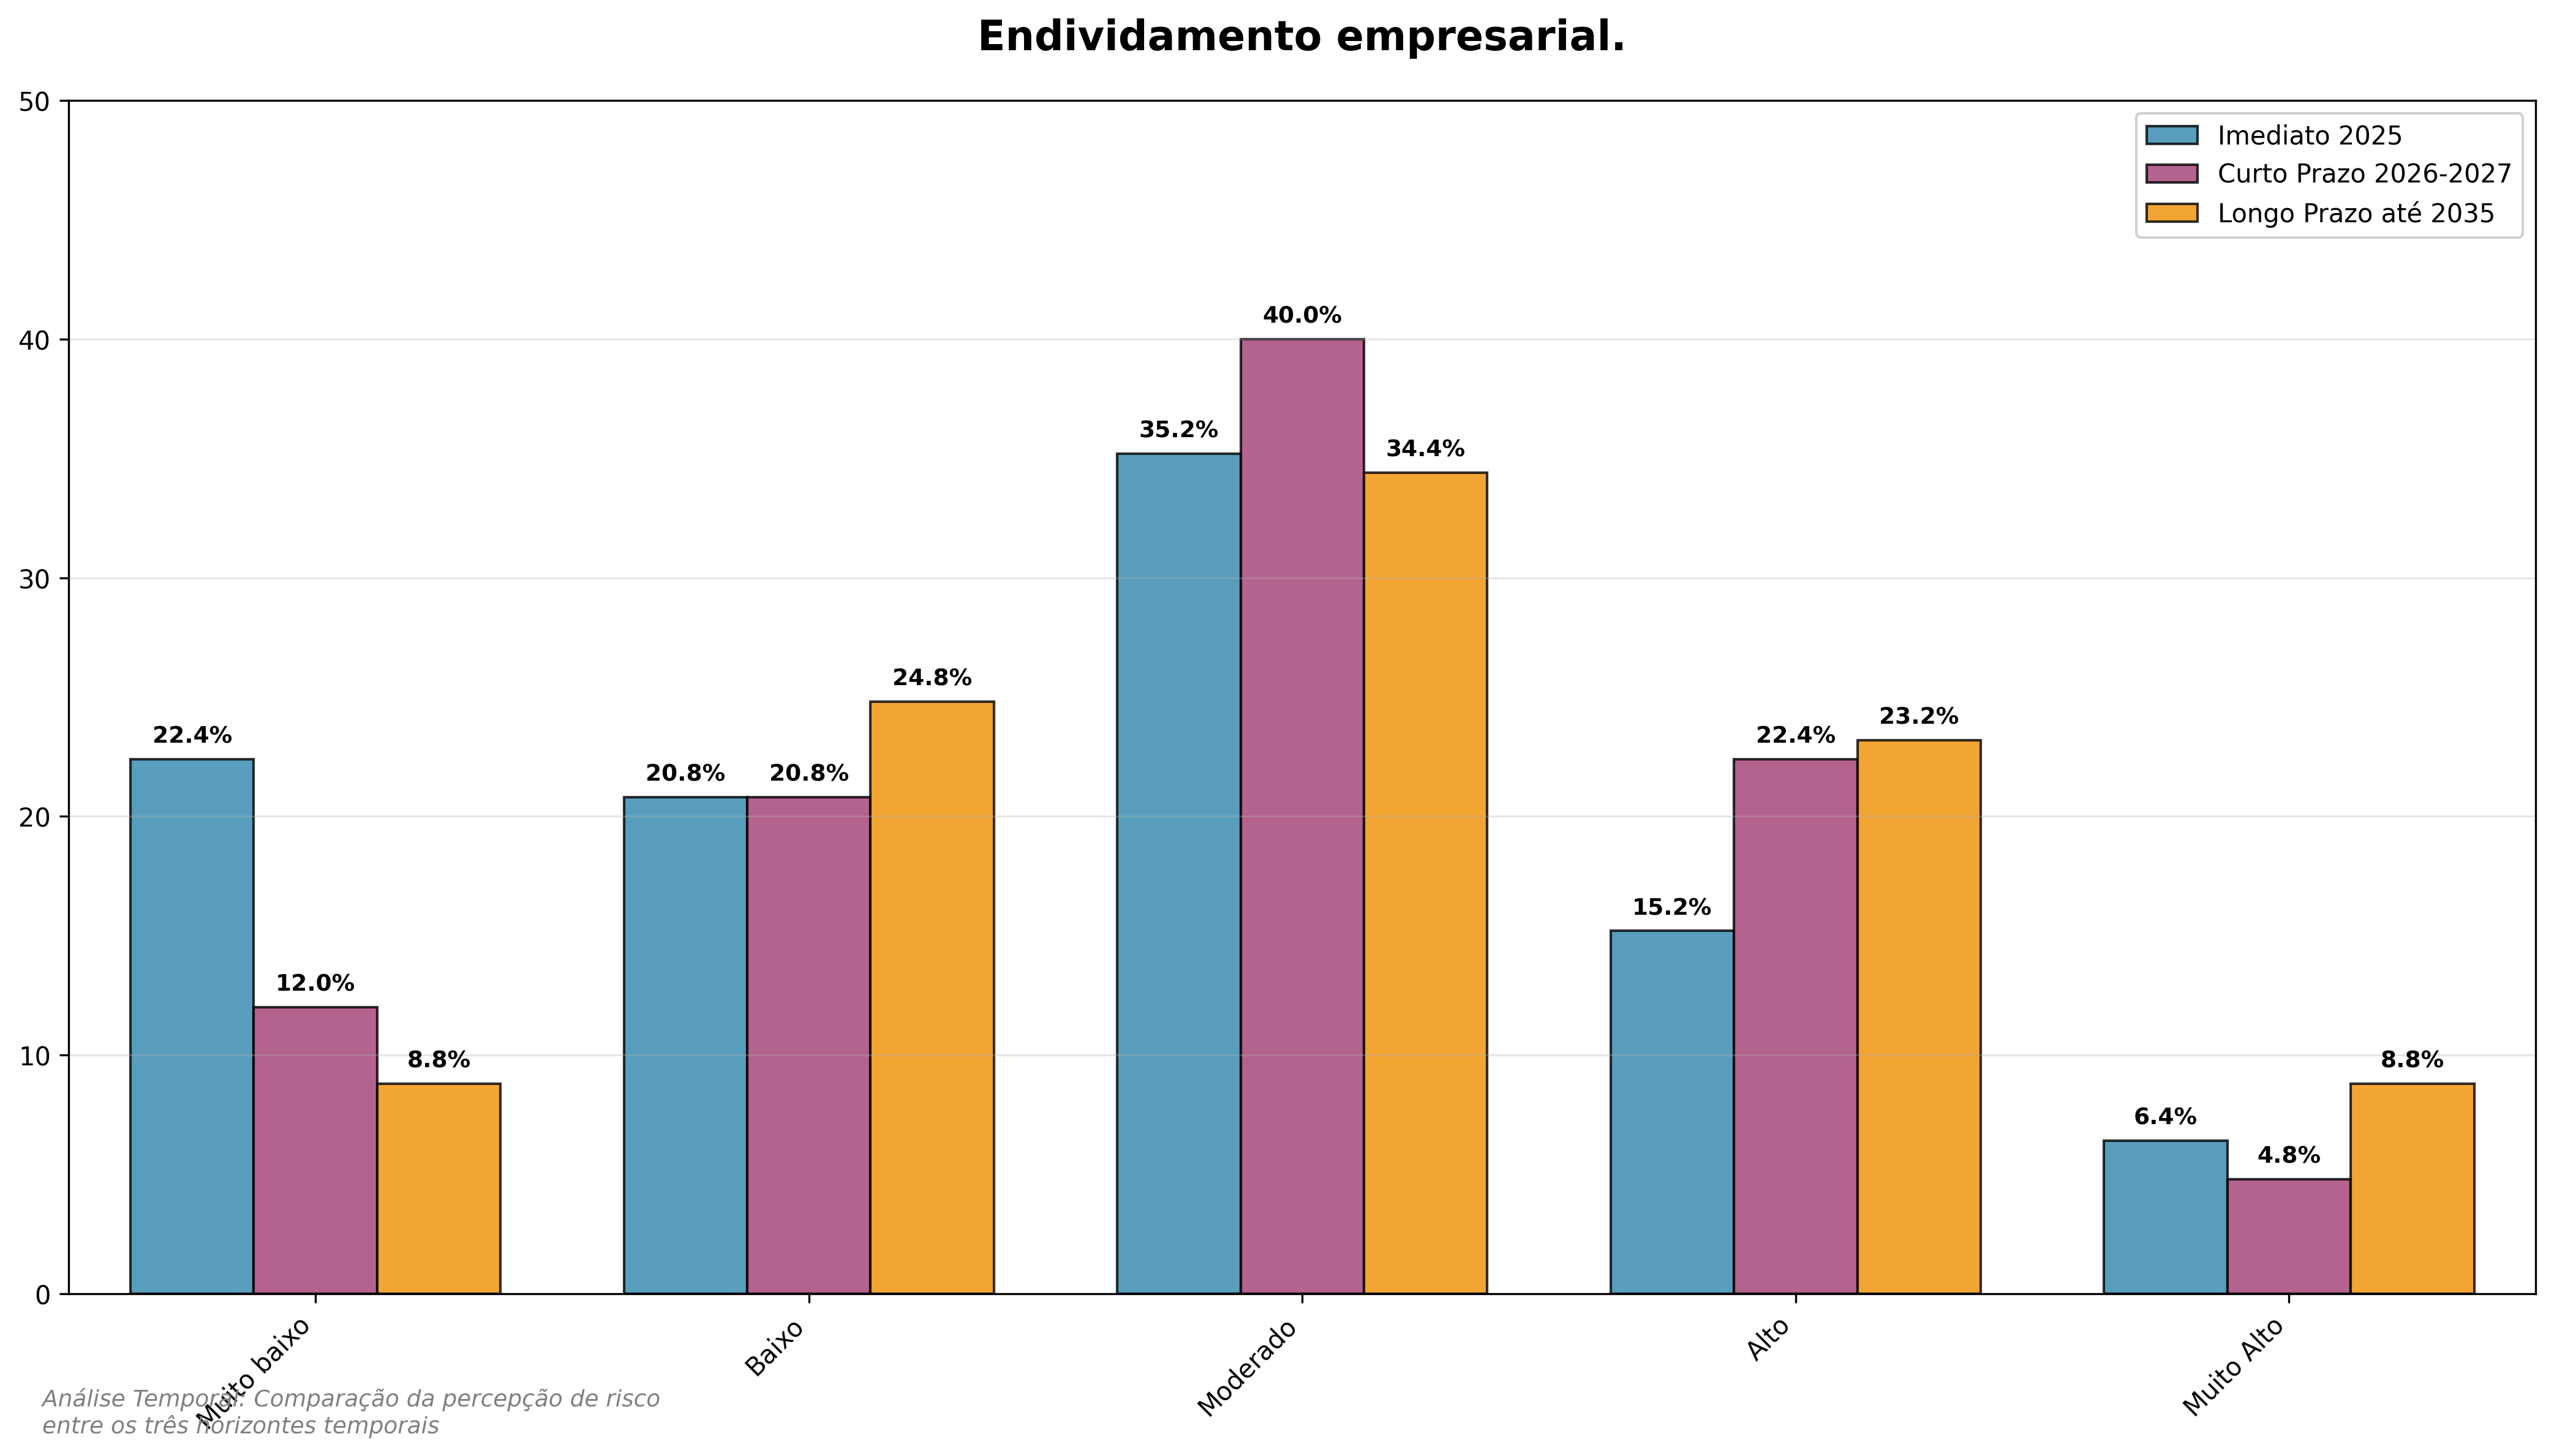
\includegraphics[keepaspectratio]{assets/economicos/grafico_agrupado_1_4_temporal.png}}

\begin{tcolorbox}[enhanced jigsaw, titlerule=0mm, colback=white, title=\textcolor{quarto-callout-tip-color}{\faLightbulb}\hspace{0.5em}{Destaques}, opacityback=0, colbacktitle=quarto-callout-tip-color!10!white, leftrule=.75mm, left=2mm, colframe=quarto-callout-tip-color-frame, bottomrule=.15mm, bottomtitle=1mm, breakable, toprule=.15mm, toptitle=1mm, opacitybacktitle=0.6, arc=.35mm, coltitle=black, rightrule=.15mm]

\textbf{Imediato (2025)}: Mediana 3.0, 22\% em risco alto

\textbf{Curto Prazo (2026-2027)}: Mediana 3.0, 27\% em risco alto

\textbf{Longo Prazo (até 2035)}: Mediana 3.0, 32\% em risco alto

\begin{itemize}
\tightlist
\item
  \textbf{Tendência}: Percepção de risco relativamente estável ao longo
  do tempo. \textbf{Endividamento empresarial. {[}Imediato (2025){]}}
\end{itemize}

Risco recorrente que se agrava com as altas taxas de juros e fontes de
financiamento de longo prazo praticamente restritas ao BNDES.
Empréstimos de curto prazo se mostram caros e impactam os resultados das
organizações.

\end{tcolorbox}

\subsection{Endividamento das pessoas}\label{endividamento-das-pessoas}

O gr?fico a seguir apresenta a evolu??o temporal do risco Endividamento
das pessoas.
\pandocbounded{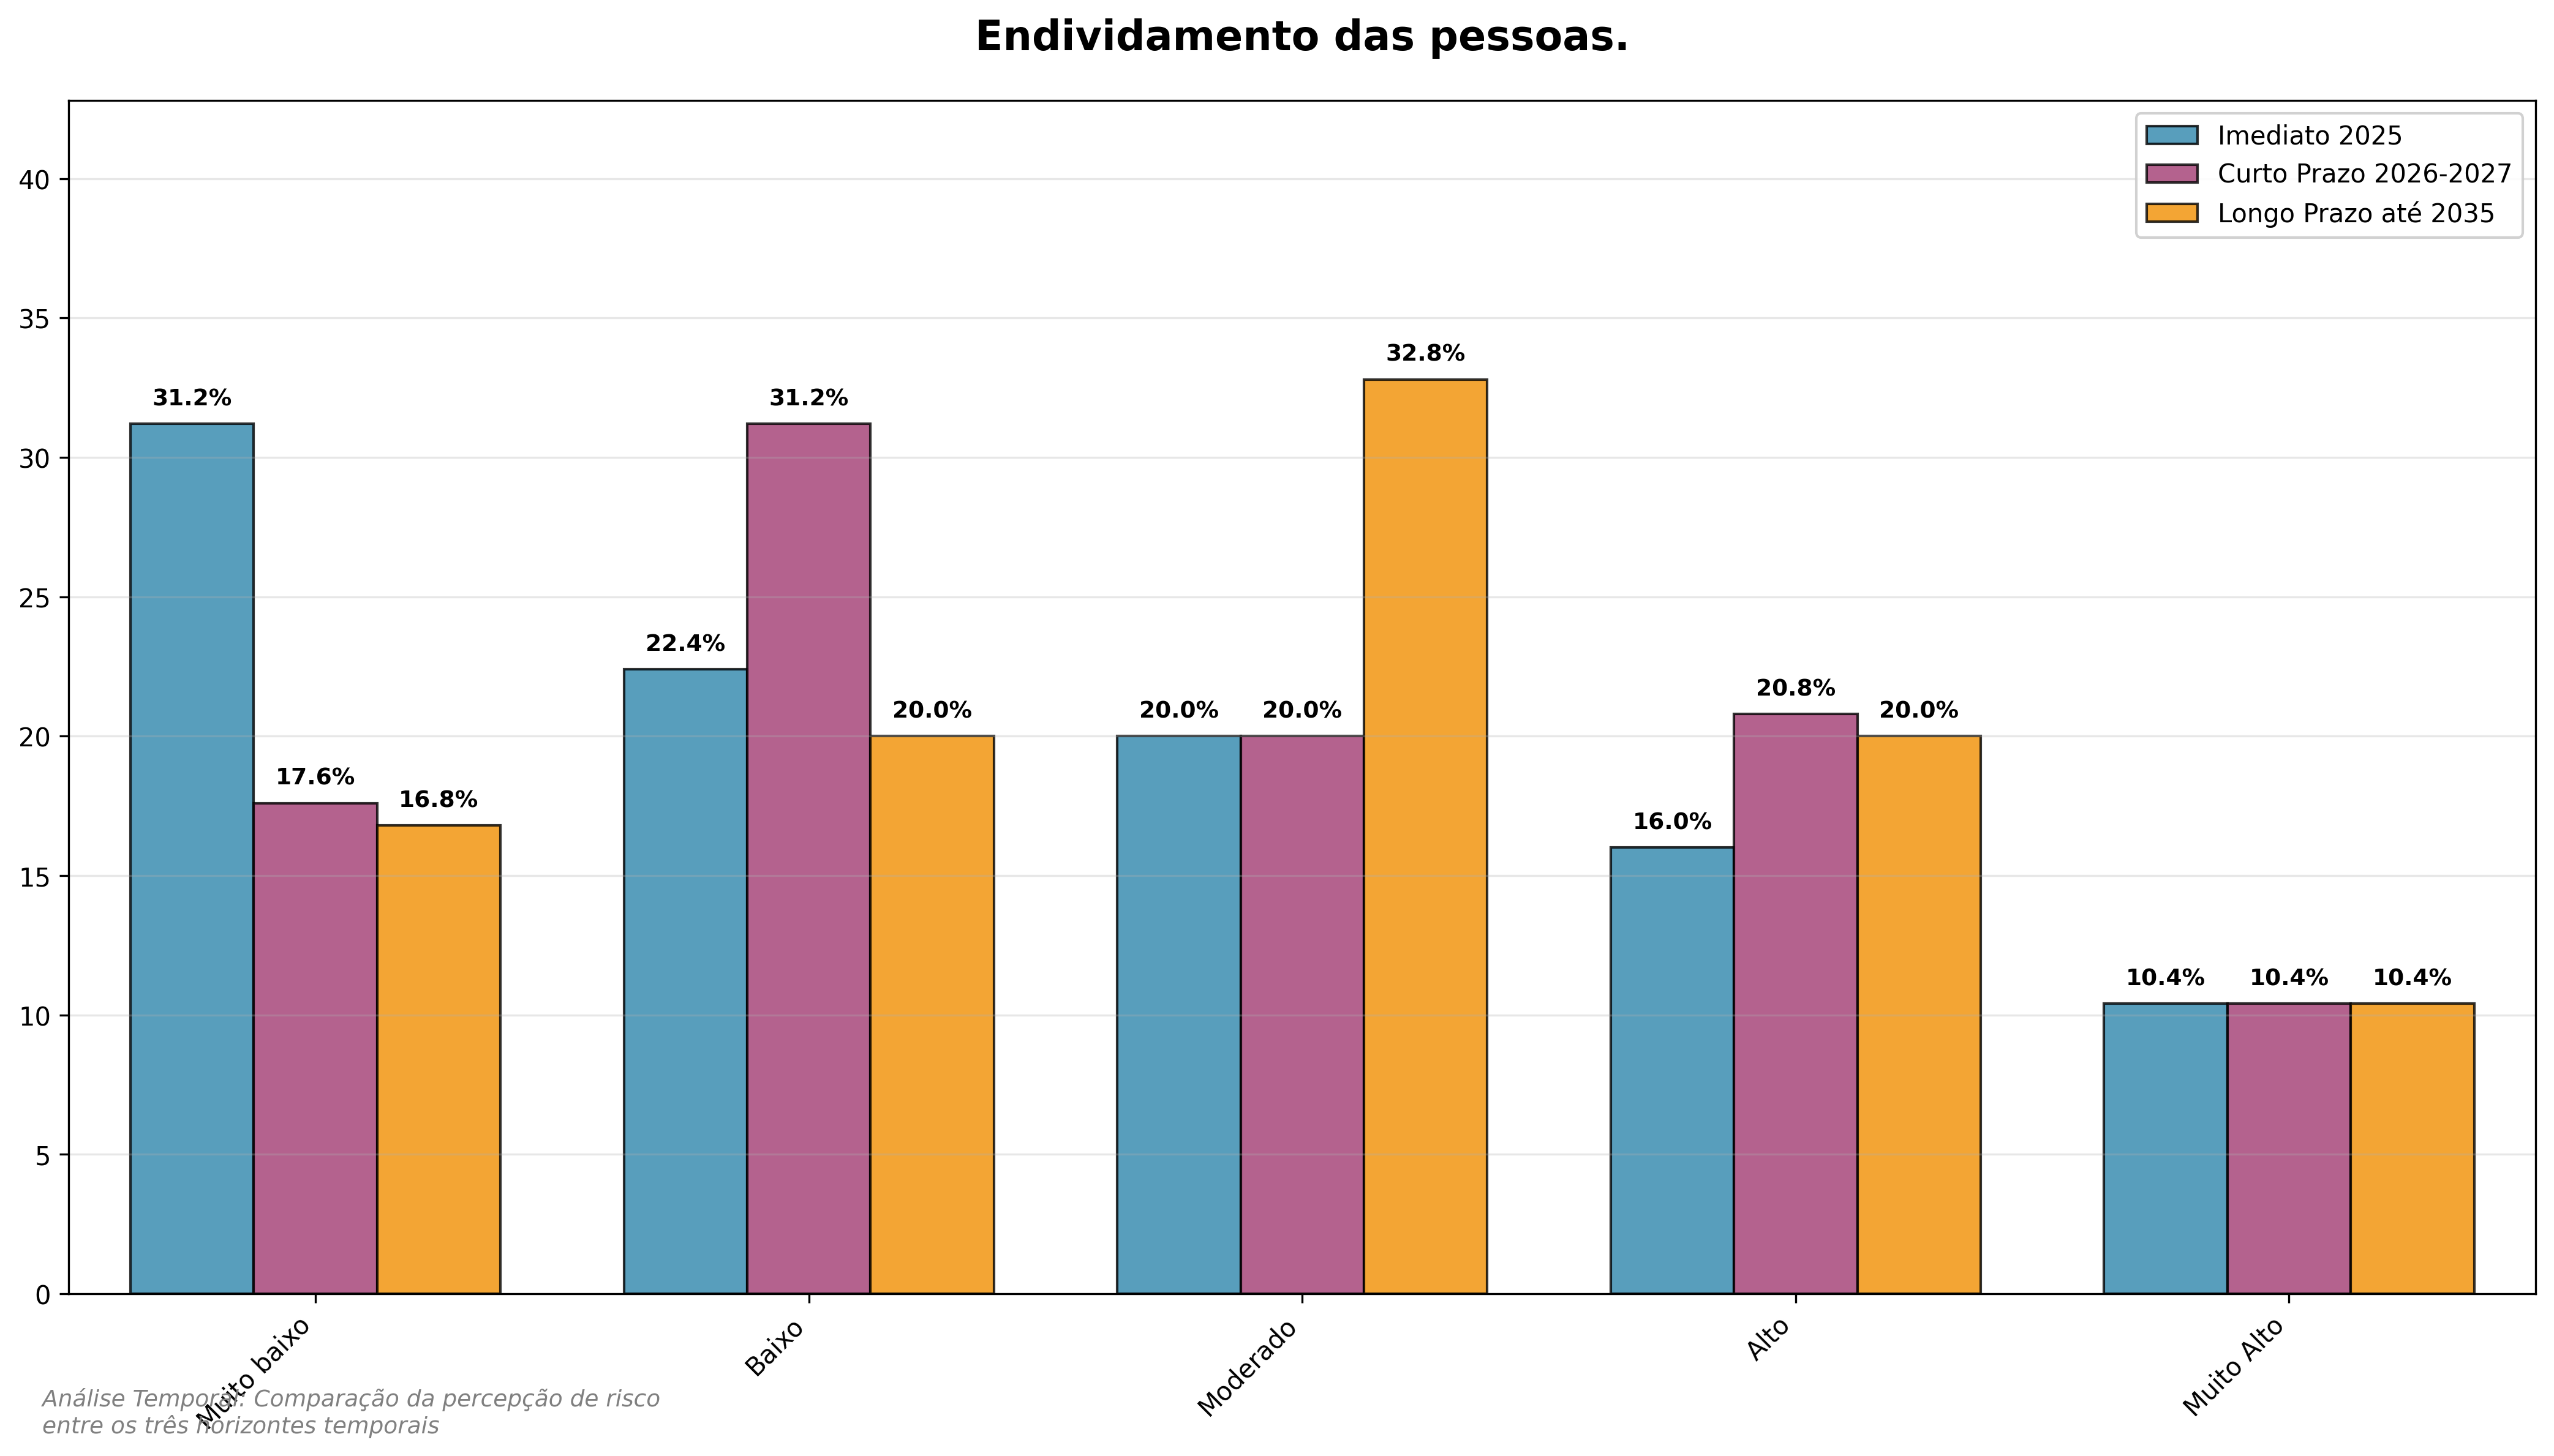
\includegraphics[keepaspectratio]{assets/economicos/grafico_agrupado_1_5_temporal.png}}

\begin{tcolorbox}[enhanced jigsaw, titlerule=0mm, colback=white, title=\textcolor{quarto-callout-tip-color}{\faLightbulb}\hspace{0.5em}{Destaques}, opacityback=0, colbacktitle=quarto-callout-tip-color!10!white, leftrule=.75mm, left=2mm, colframe=quarto-callout-tip-color-frame, bottomrule=.15mm, bottomtitle=1mm, breakable, toprule=.15mm, toptitle=1mm, opacitybacktitle=0.6, arc=.35mm, coltitle=black, rightrule=.15mm]

\textbf{Imediato (2025)}: Mediana 2.0, 26\% em risco alto

\textbf{Curto Prazo (2026-2027)}: Mediana 3.0, 31\% em risco alto

\textbf{Longo Prazo (até 2035)}: Mediana 3.0, 30\% em risco alto

\begin{itemize}
\tightlist
\item
  \textbf{Tendência}: Percepção de risco relativamente estável ao longo
  do tempo. \textbf{Endividamento das pessoas.}
\end{itemize}

Risco decorrente da exposição das pessoas às condições de tomada de
recursos por demais exigentes e custosas. Políticas de recomposição de
suas rendas podem aliviar essa situação endêmica para parte significante
da população.

\end{tcolorbox}

\subsection{Falhas, interrupções ou disrupções em cadeias de suprimentos
relevantes}\label{falhas-interrupuxe7uxf5es-ou-disrupuxe7uxf5es-em-cadeias-de-suprimentos-relevantes}

O gr?fico a seguir apresenta a evolu??o temporal do risco Falhas,
interrupções ou disrupções em cadeias de suprimentos relevantes.
\pandocbounded{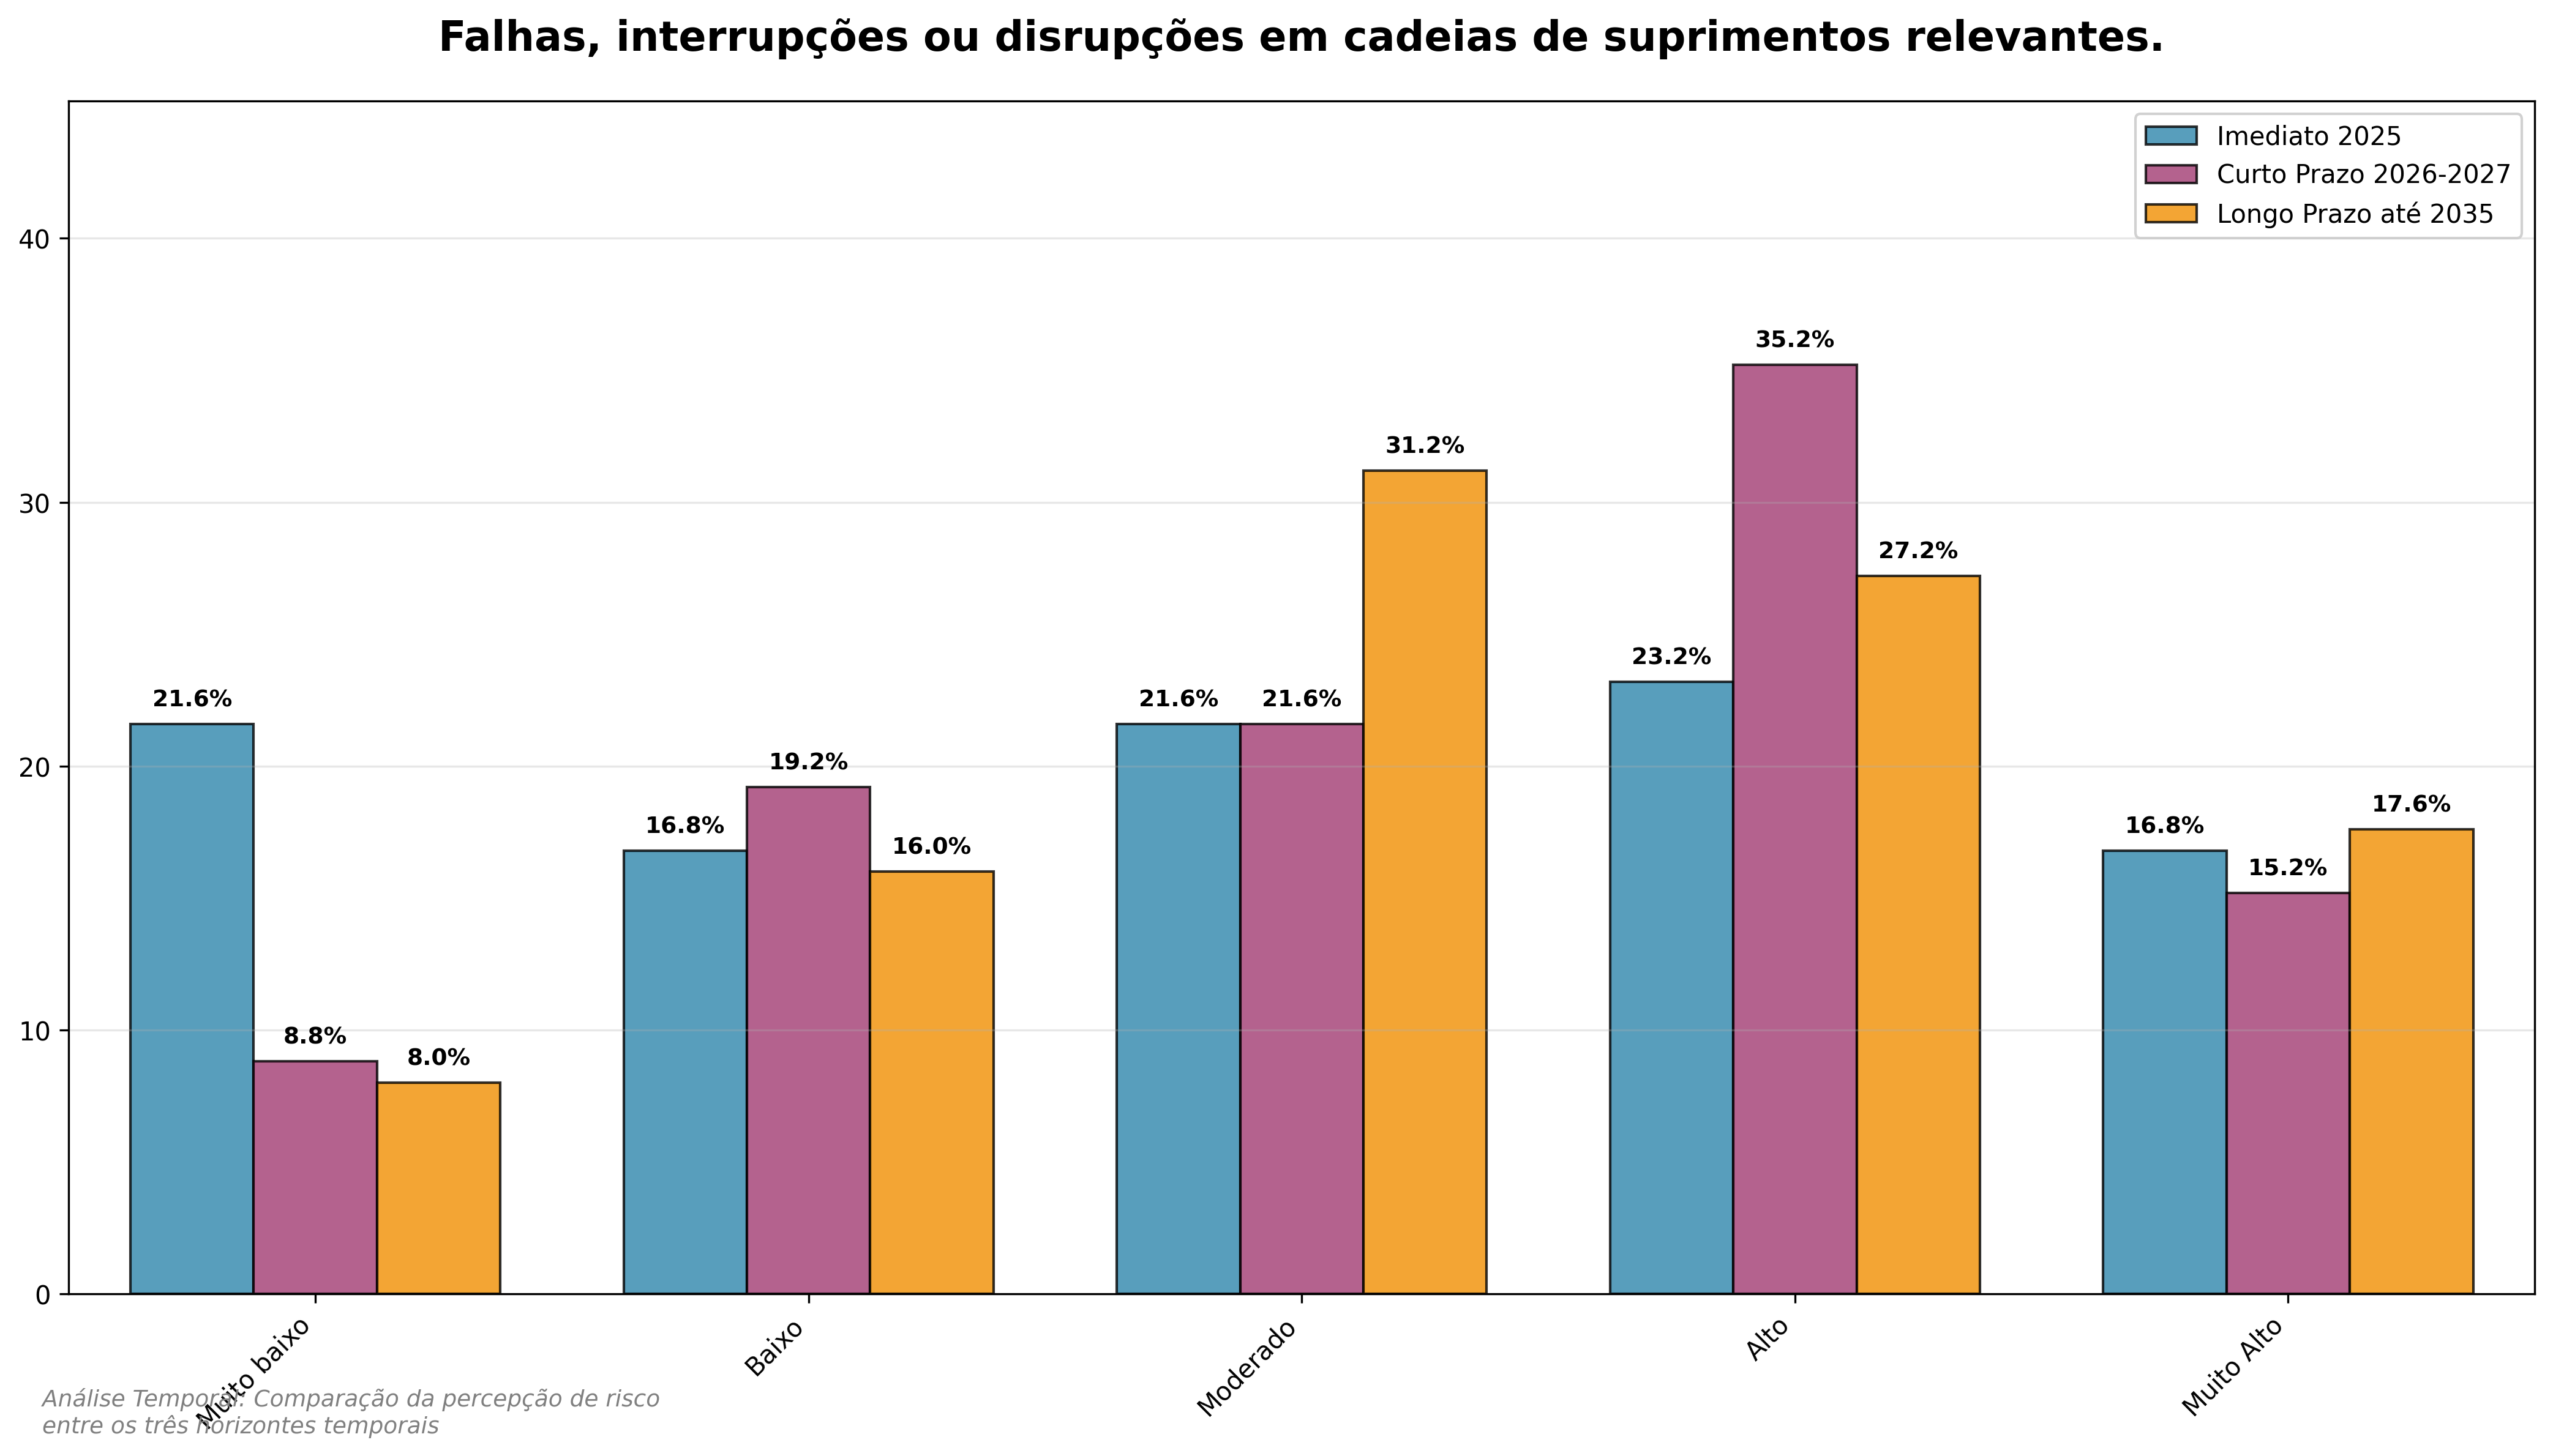
\includegraphics[keepaspectratio]{assets/economicos/grafico_agrupado_1_6_temporal.png}}

\begin{tcolorbox}[enhanced jigsaw, titlerule=0mm, colback=white, title=\textcolor{quarto-callout-tip-color}{\faLightbulb}\hspace{0.5em}{Destaques}, opacityback=0, colbacktitle=quarto-callout-tip-color!10!white, leftrule=.75mm, left=2mm, colframe=quarto-callout-tip-color-frame, bottomrule=.15mm, bottomtitle=1mm, breakable, toprule=.15mm, toptitle=1mm, opacitybacktitle=0.6, arc=.35mm, coltitle=black, rightrule=.15mm]

\textbf{Imediato (2025)}: Mediana 3.0, 40\% em risco alto

\textbf{Curto Prazo (2026-2027)}: Mediana 4.0, 50\% em risco alto

\textbf{Longo Prazo (até 2035)}: Mediana 3.0, 45\% em risco alto

\begin{itemize}
\tightlist
\item
  \textbf{Tendência}: Pico de risco no curto prazo, retornando ao nível
  inicial. \textbf{Falhas, interrupções ou disrupções em cadeias de
  suprimentos relevantes.}
\end{itemize}

Riscos que podem advir de causas naturais e/ou de políticas restritivas
ou mesmo impeditivas de operações comerciais como a praticada pelo atual
governo estadunidense. Portos fazem parte de cadeias logísticas e têm de
estar alerta para a evolução das cadeias produtivas de seus usuários
e/ou parceiros.

\end{tcolorbox}

\subsection{Disrupções em infraestruturas críticas (físicas e digitais)
ou serviços que sustentam sistemas
críticos}\label{disrupuxe7uxf5es-em-infraestruturas-cruxedticas-fuxedsicas-e-digitais-ou-serviuxe7os-que-sustentam-sistemas-cruxedticos}

O gr?fico a seguir apresenta a evolu??o temporal do risco Disrupções em
infraestruturas críticas (físicas e digitais) ou serviços que sustentam
sistemas críticos.
\pandocbounded{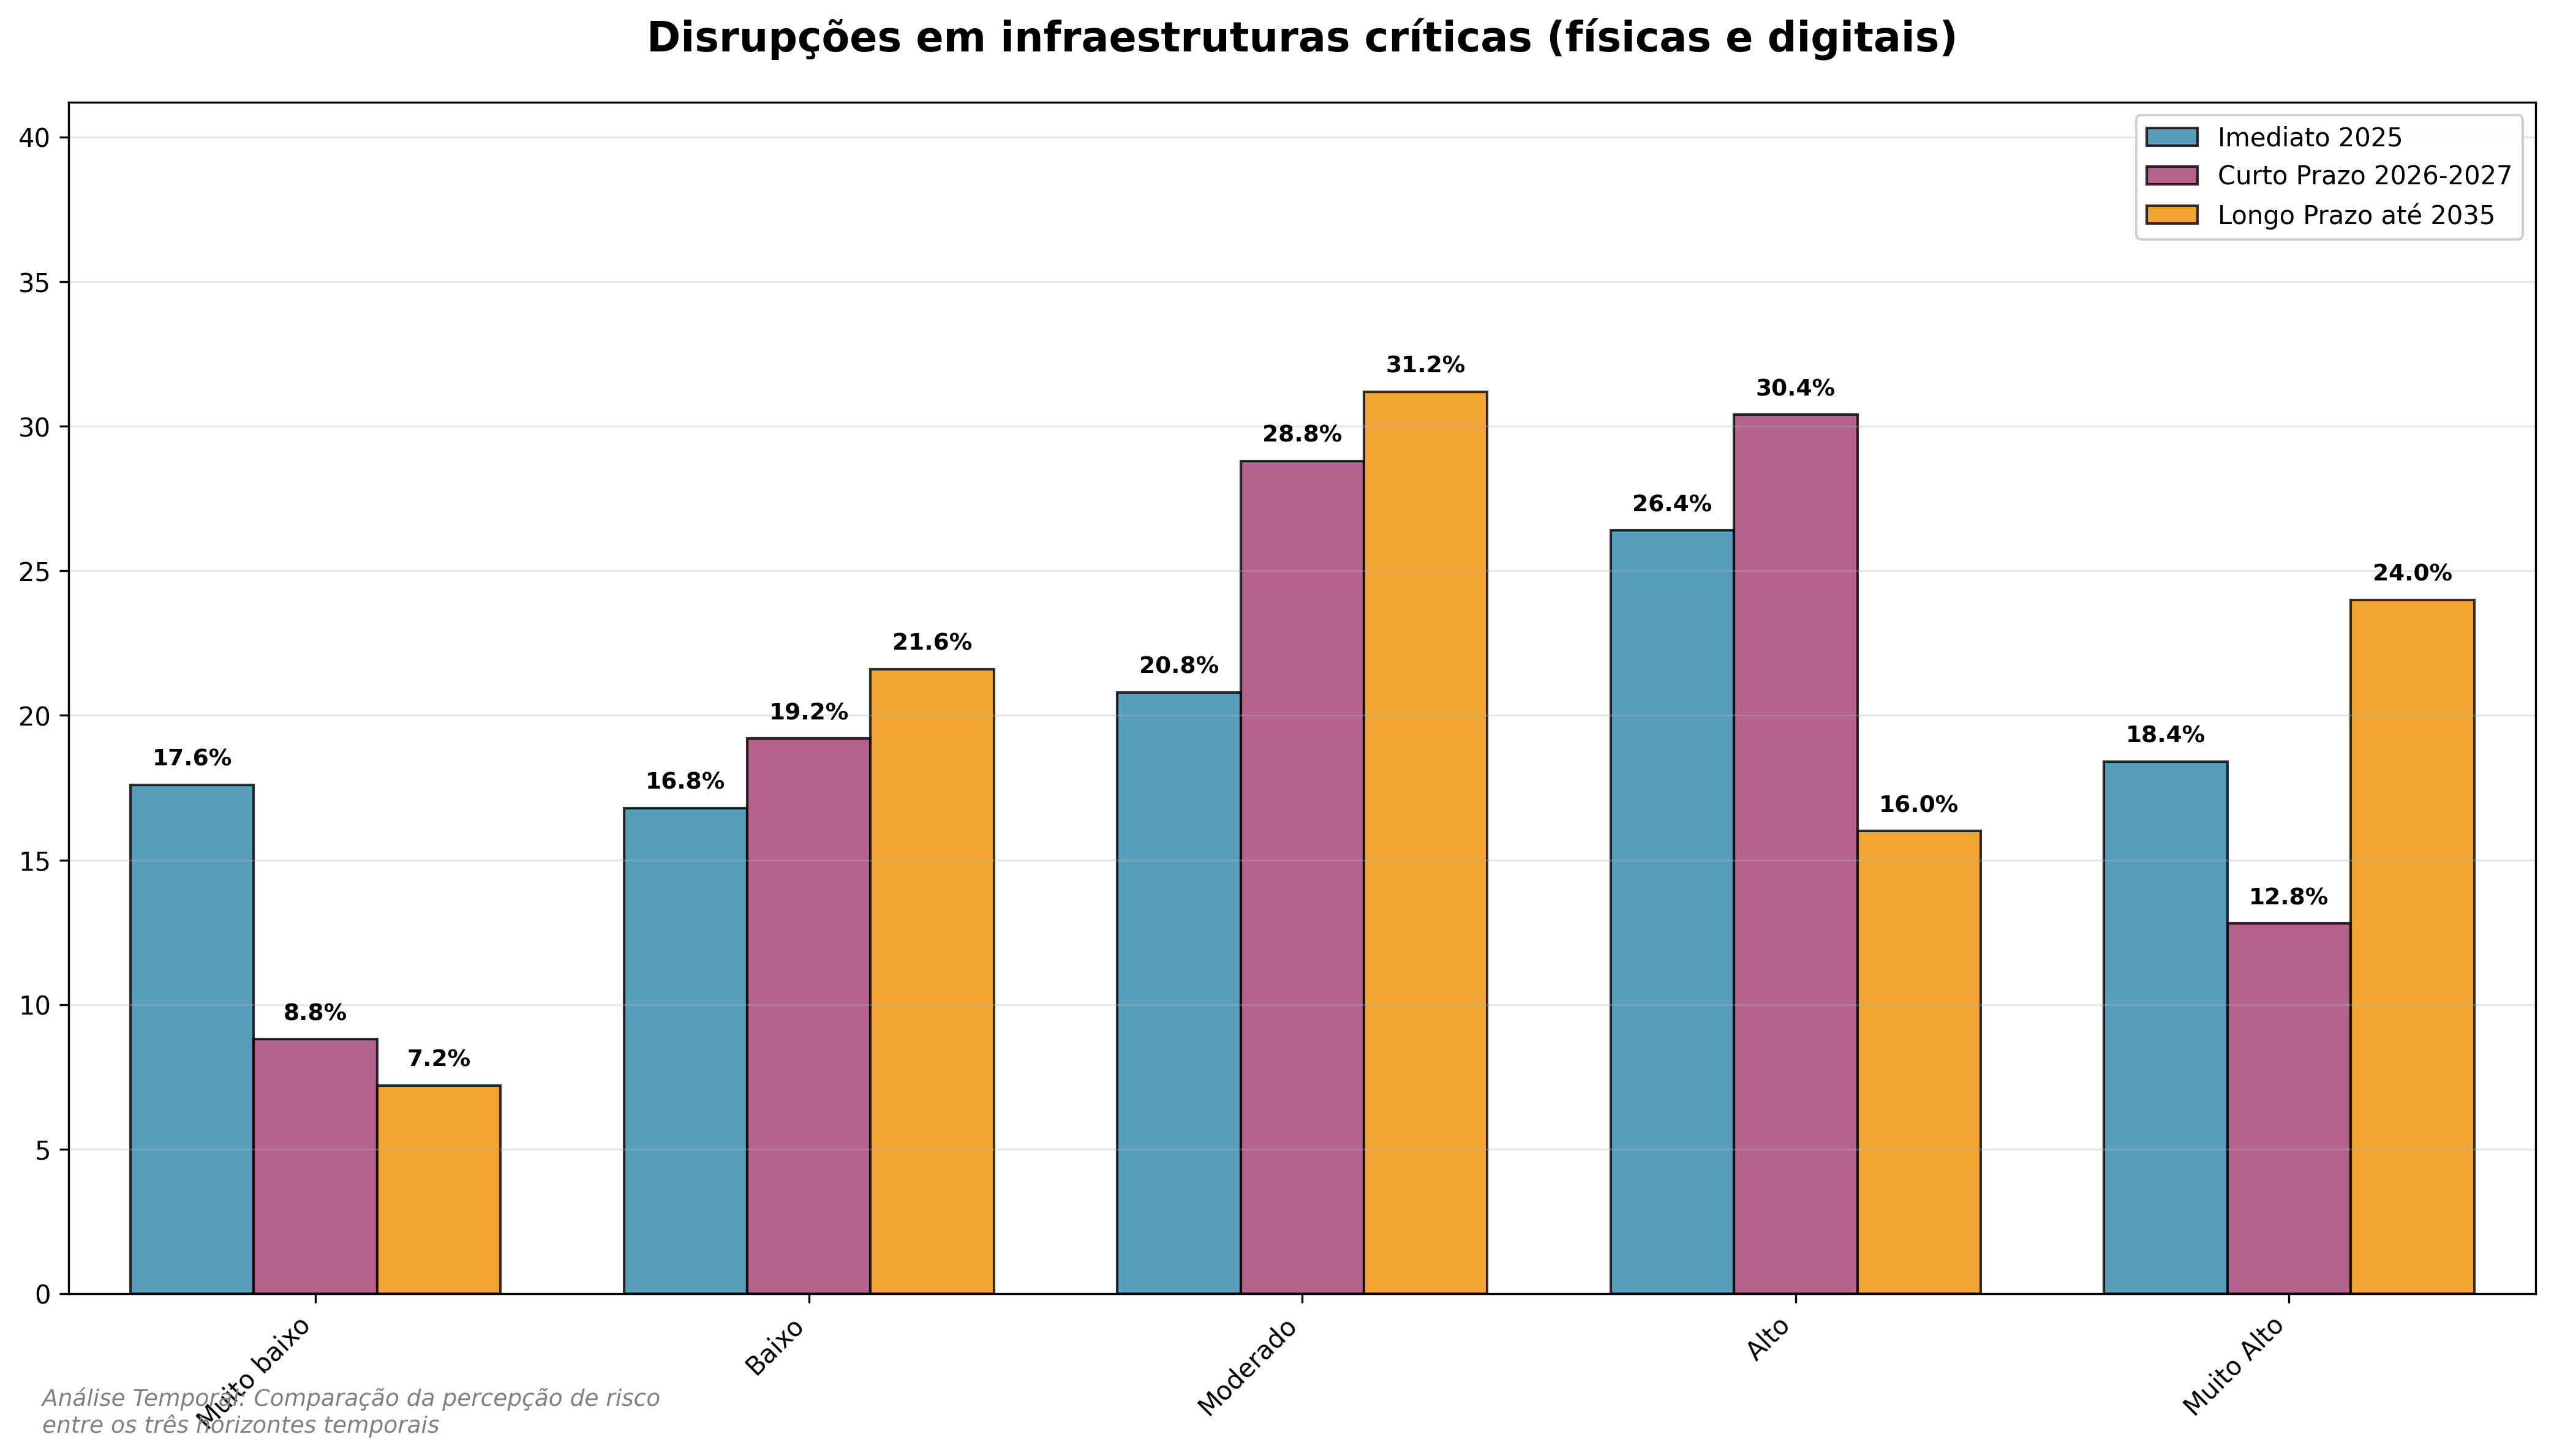
\includegraphics[keepaspectratio]{assets/economicos/grafico_agrupado_1_7_temporal.png}}

\begin{tcolorbox}[enhanced jigsaw, titlerule=0mm, colback=white, title=\textcolor{quarto-callout-tip-color}{\faLightbulb}\hspace{0.5em}{Destaques}, opacityback=0, colbacktitle=quarto-callout-tip-color!10!white, leftrule=.75mm, left=2mm, colframe=quarto-callout-tip-color-frame, bottomrule=.15mm, bottomtitle=1mm, breakable, toprule=.15mm, toptitle=1mm, opacitybacktitle=0.6, arc=.35mm, coltitle=black, rightrule=.15mm]

\textbf{Imediato (2025)}: Mediana 3.0, 45\% em risco alto

\textbf{Curto Prazo (2026-2027)}: Mediana 3.0, 43\% em risco alto

\textbf{Longo Prazo (até 2035)}: Mediana 3.0, 40\% em risco alto

\begin{itemize}
\tightlist
\item
  \textbf{Tendência}: Percepção de risco relativamente estável ao longo
  do tempo. \textbf{Disrupções em infraestruturas críticas (físicas e
  digitais) ou serviços que sustentam sistemas críticos (internet,
  telecomunicações, serviços públicos, sistemas financeiros ou
  energia).}
\end{itemize}

Este risco é constante e, a exemplo do de falhas nas cadeias de
suprimentos (Risco 1.6), exige acompanhamento que se estende para além
do ambiente portuário, pois a evolução tecnológica digital tem sido
intensa e disruptiva. Portos devem contar com áreas de acompanhamento e
adaptação das inovações às suas operações. É crítico o seu impacto na
geração e alocação de postos de trabalho e renda dos trabalhadores.

\end{tcolorbox}

\subsection{Diminuição (estagnação) do ritmo e da dinâmica das
atividades
econômicas}\label{diminuiuxe7uxe3o-estagnauxe7uxe3o-do-ritmo-e-da-dinuxe2mica-das-atividades-econuxf4micas}

O gr?fico a seguir apresenta a evolu??o temporal do risco Diminuição
(estagnação) do ritmo e da dinâmica das atividades econômicas.
\pandocbounded{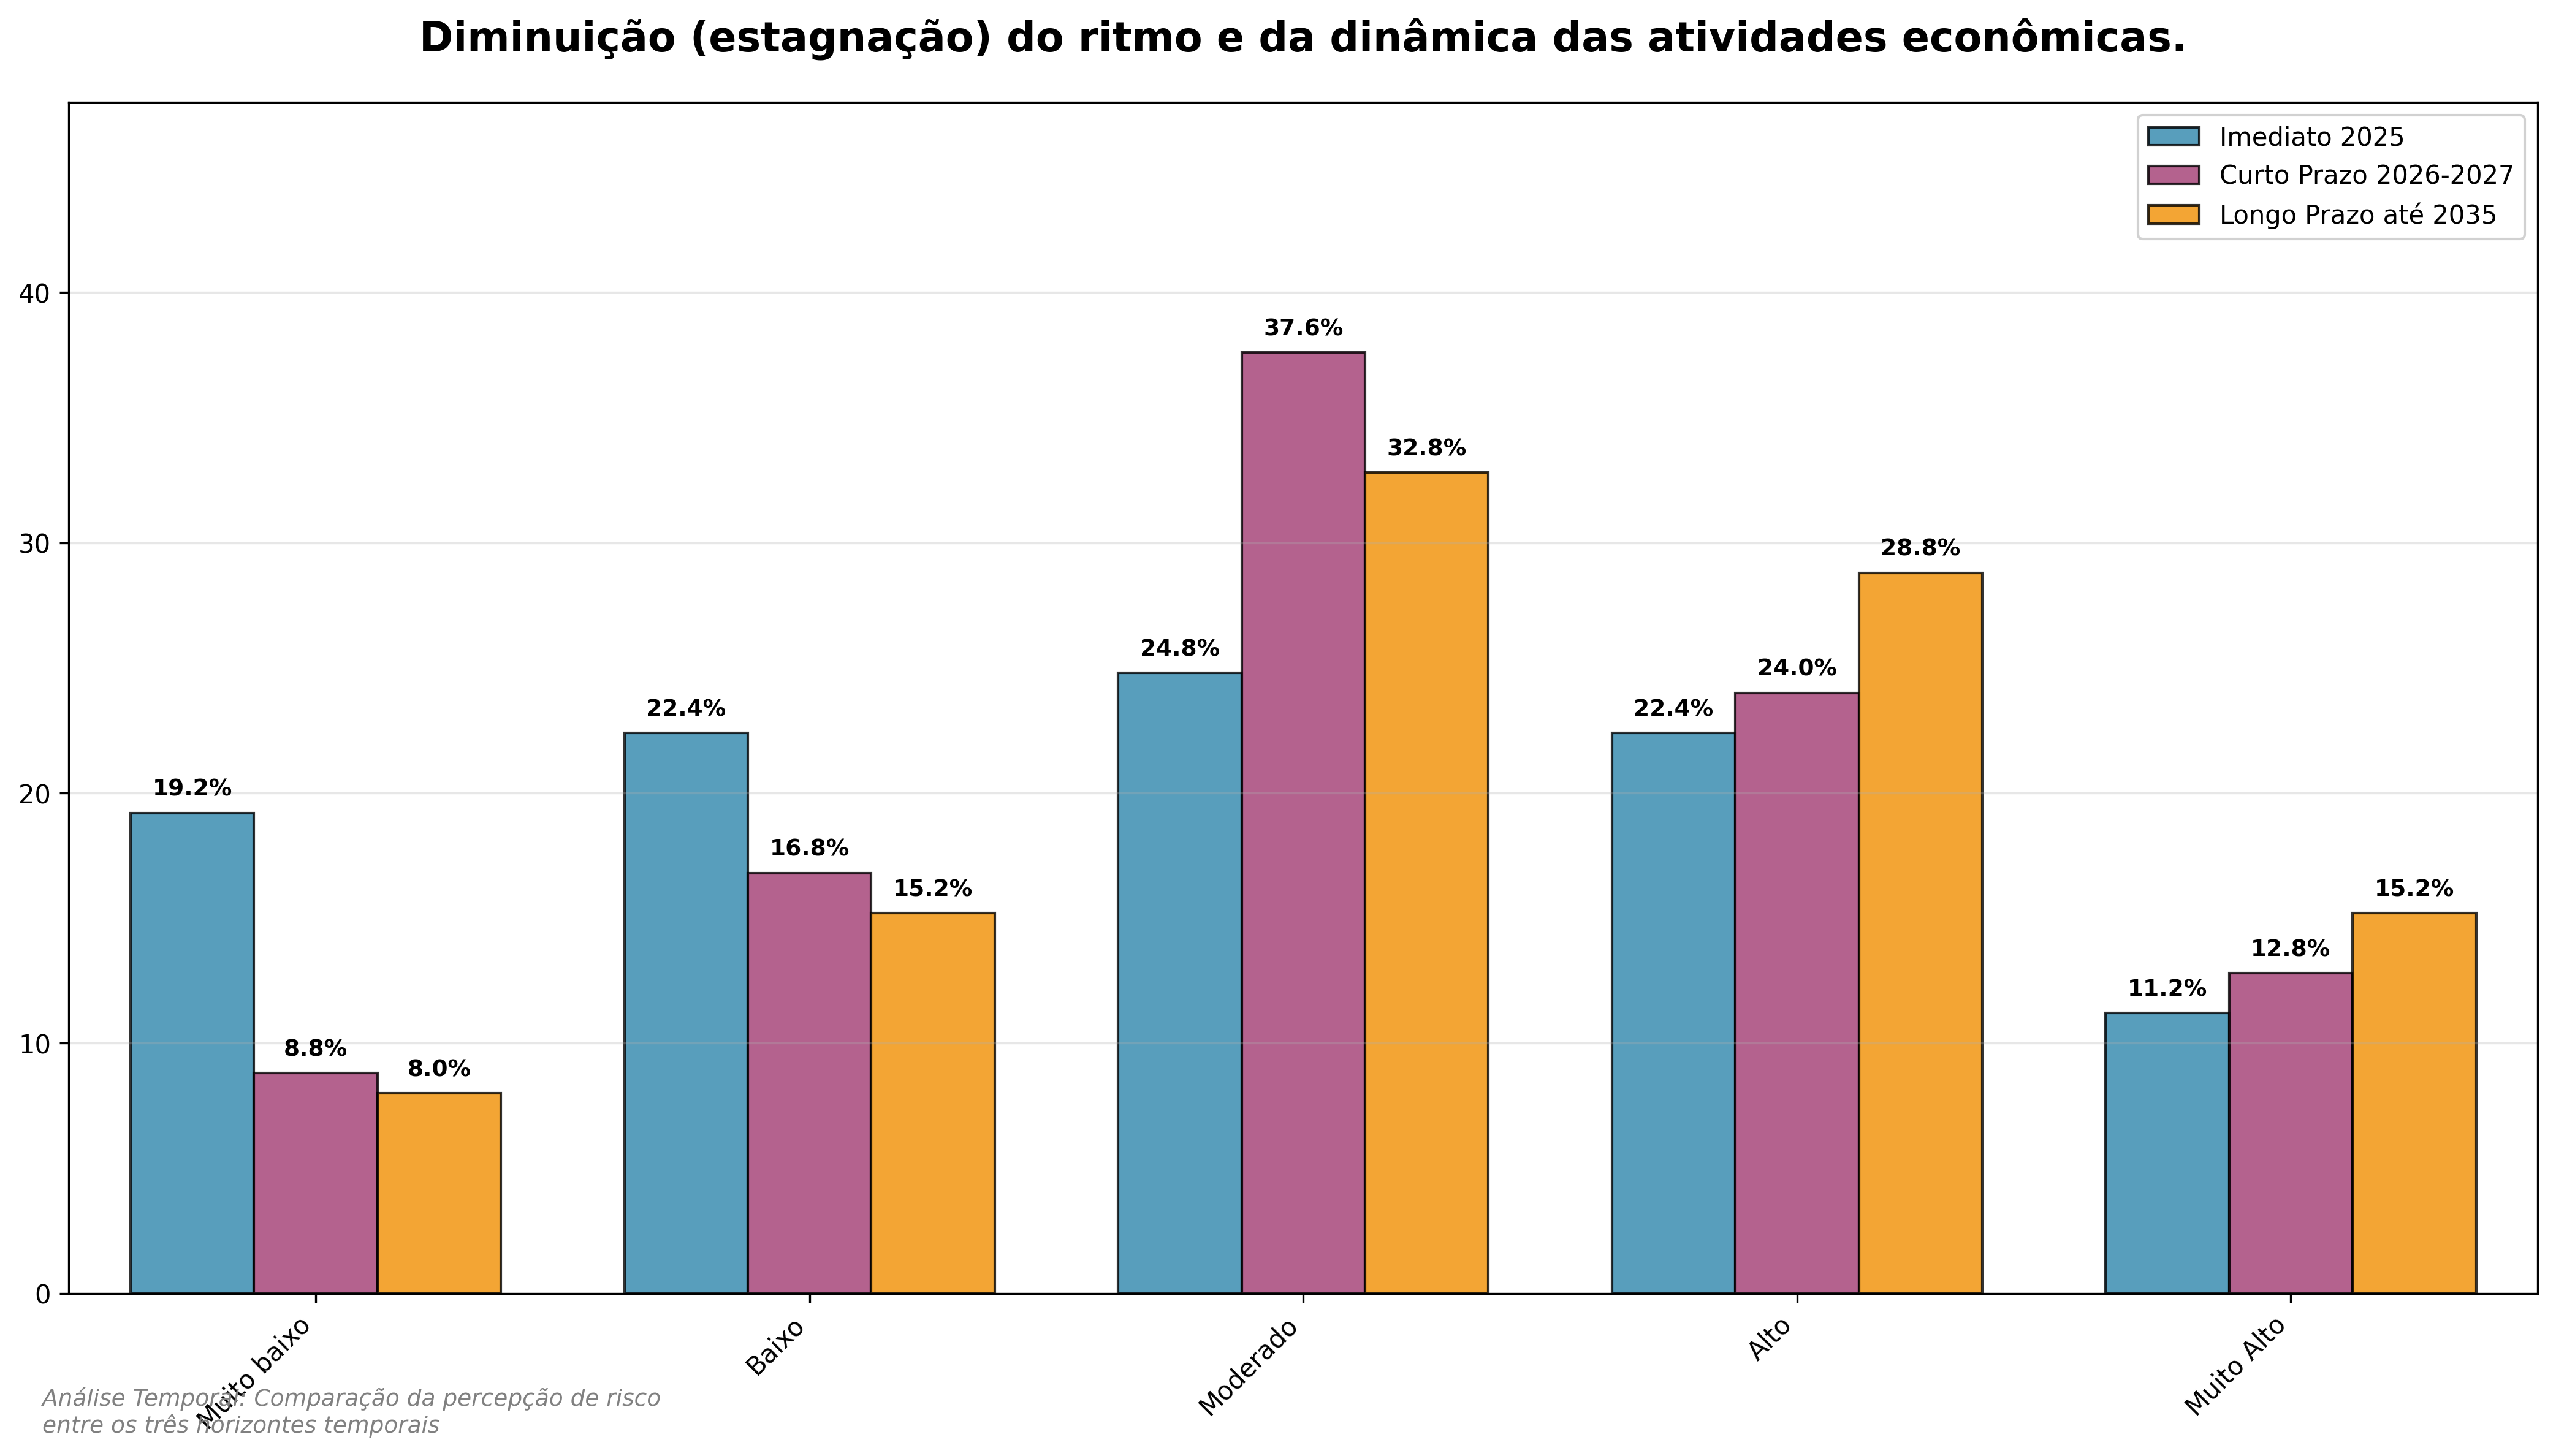
\includegraphics[keepaspectratio]{assets/economicos/grafico_agrupado_1_8_temporal.png}}

\begin{tcolorbox}[enhanced jigsaw, titlerule=0mm, colback=white, title=\textcolor{quarto-callout-tip-color}{\faLightbulb}\hspace{0.5em}{Destaques}, opacityback=0, colbacktitle=quarto-callout-tip-color!10!white, leftrule=.75mm, left=2mm, colframe=quarto-callout-tip-color-frame, bottomrule=.15mm, bottomtitle=1mm, breakable, toprule=.15mm, toptitle=1mm, opacitybacktitle=0.6, arc=.35mm, coltitle=black, rightrule=.15mm]

\textbf{Imediato (2025)}: Mediana 3.0, 34\% em risco alto

\textbf{Curto Prazo (2026-2027)}: Mediana 3.0, 37\% em risco alto

\textbf{Longo Prazo (até 2035)}: Mediana 3.0, 44\% em risco alto

\begin{itemize}
\tightlist
\item
  \textbf{Tendência}: Percepção de risco relativamente estável ao longo
  do tempo. \textbf{Diminuição (estagnação) do ritmo e da dinâmica das
  atividades econômicas.}
\end{itemize}

Este risco é mais uma consequência do que uma causa, pois ciclos
econômicos e setoriais se repetem. Entende-se que diminuição do ritmo
não corresponde a retração ou perda de atividades econômicas.

\end{tcolorbox}

\subsection{Ação do crime organizado e atividades ilícitas de empresas e
pessoas}\label{auxe7uxe3o-do-crime-organizado-e-atividades-iluxedcitas-de-empresas-e-pessoas}

O gr?fico a seguir apresenta a evolu??o temporal do risco Ação do crime
organizado e atividades ilícitas de empresas e pessoas.
\pandocbounded{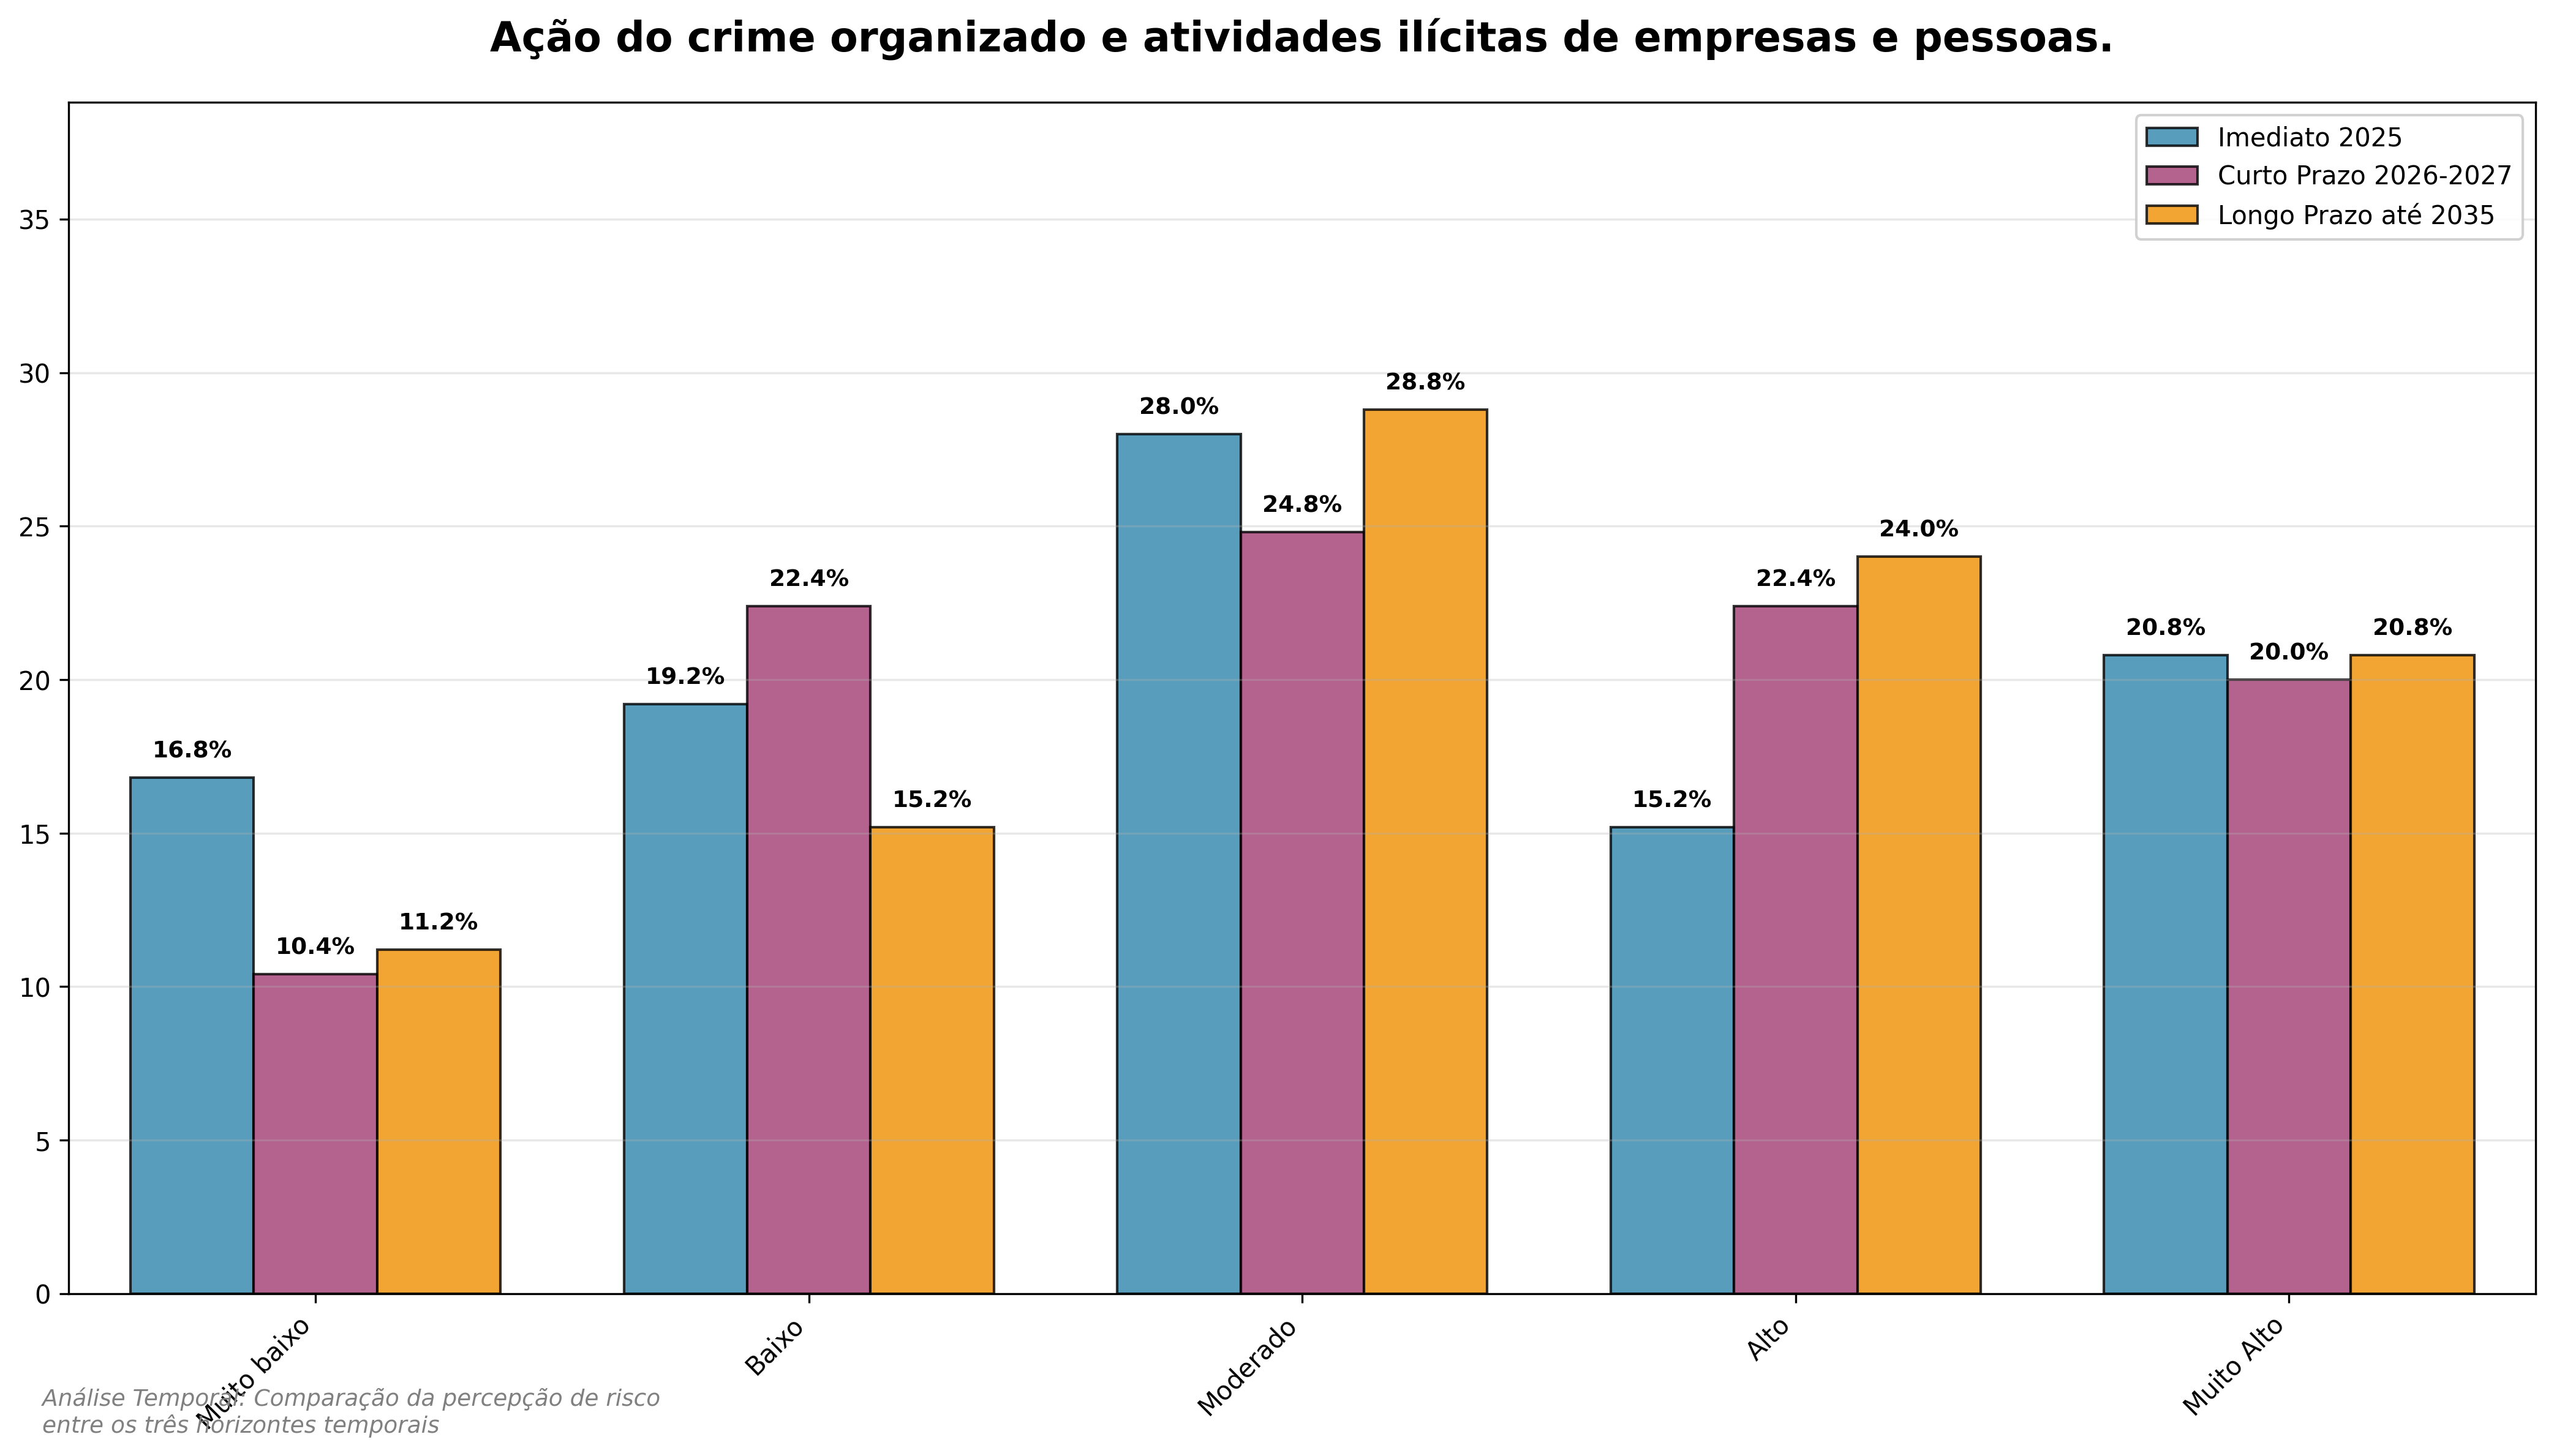
\includegraphics[keepaspectratio]{assets/economicos/grafico_agrupado_1_9_temporal.png}}

\begin{tcolorbox}[enhanced jigsaw, titlerule=0mm, colback=white, title=\textcolor{quarto-callout-tip-color}{\faLightbulb}\hspace{0.5em}{Destaques}, opacityback=0, colbacktitle=quarto-callout-tip-color!10!white, leftrule=.75mm, left=2mm, colframe=quarto-callout-tip-color-frame, bottomrule=.15mm, bottomtitle=1mm, breakable, toprule=.15mm, toptitle=1mm, opacitybacktitle=0.6, arc=.35mm, coltitle=black, rightrule=.15mm]

\textbf{Imediato (2025)}: Mediana 3.0, 36\% em risco alto

\textbf{Curto Prazo (2026-2027)}: Mediana 3.0, 42\% em risco alto

\textbf{Longo Prazo (até 2035)}: Mediana 3.0, 45\% em risco alto

\begin{itemize}
\tightlist
\item
  \textbf{Tendência}: Percepção de risco relativamente estável ao longo
  do tempo. \textbf{Ação do crime organizado e atividades ilícitas de
  empresas e pessoas.}
\end{itemize}

Risco crítico e permanente nas operações portuárias. Portos são portas
de entrada e saída de materiais ilegais (drogas, armas e contrabandos).
A vigilância deve ser constante e permanente com atuação de autoridades
policiais, da Marinha e das Aduanas e das polícias portuárias.

\end{tcolorbox}

\subsection{Aumento da inflação}\label{aumento-da-inflauxe7uxe3o}

O gr?fico a seguir apresenta a evolu??o temporal do risco Aumento da
inflação.
\pandocbounded{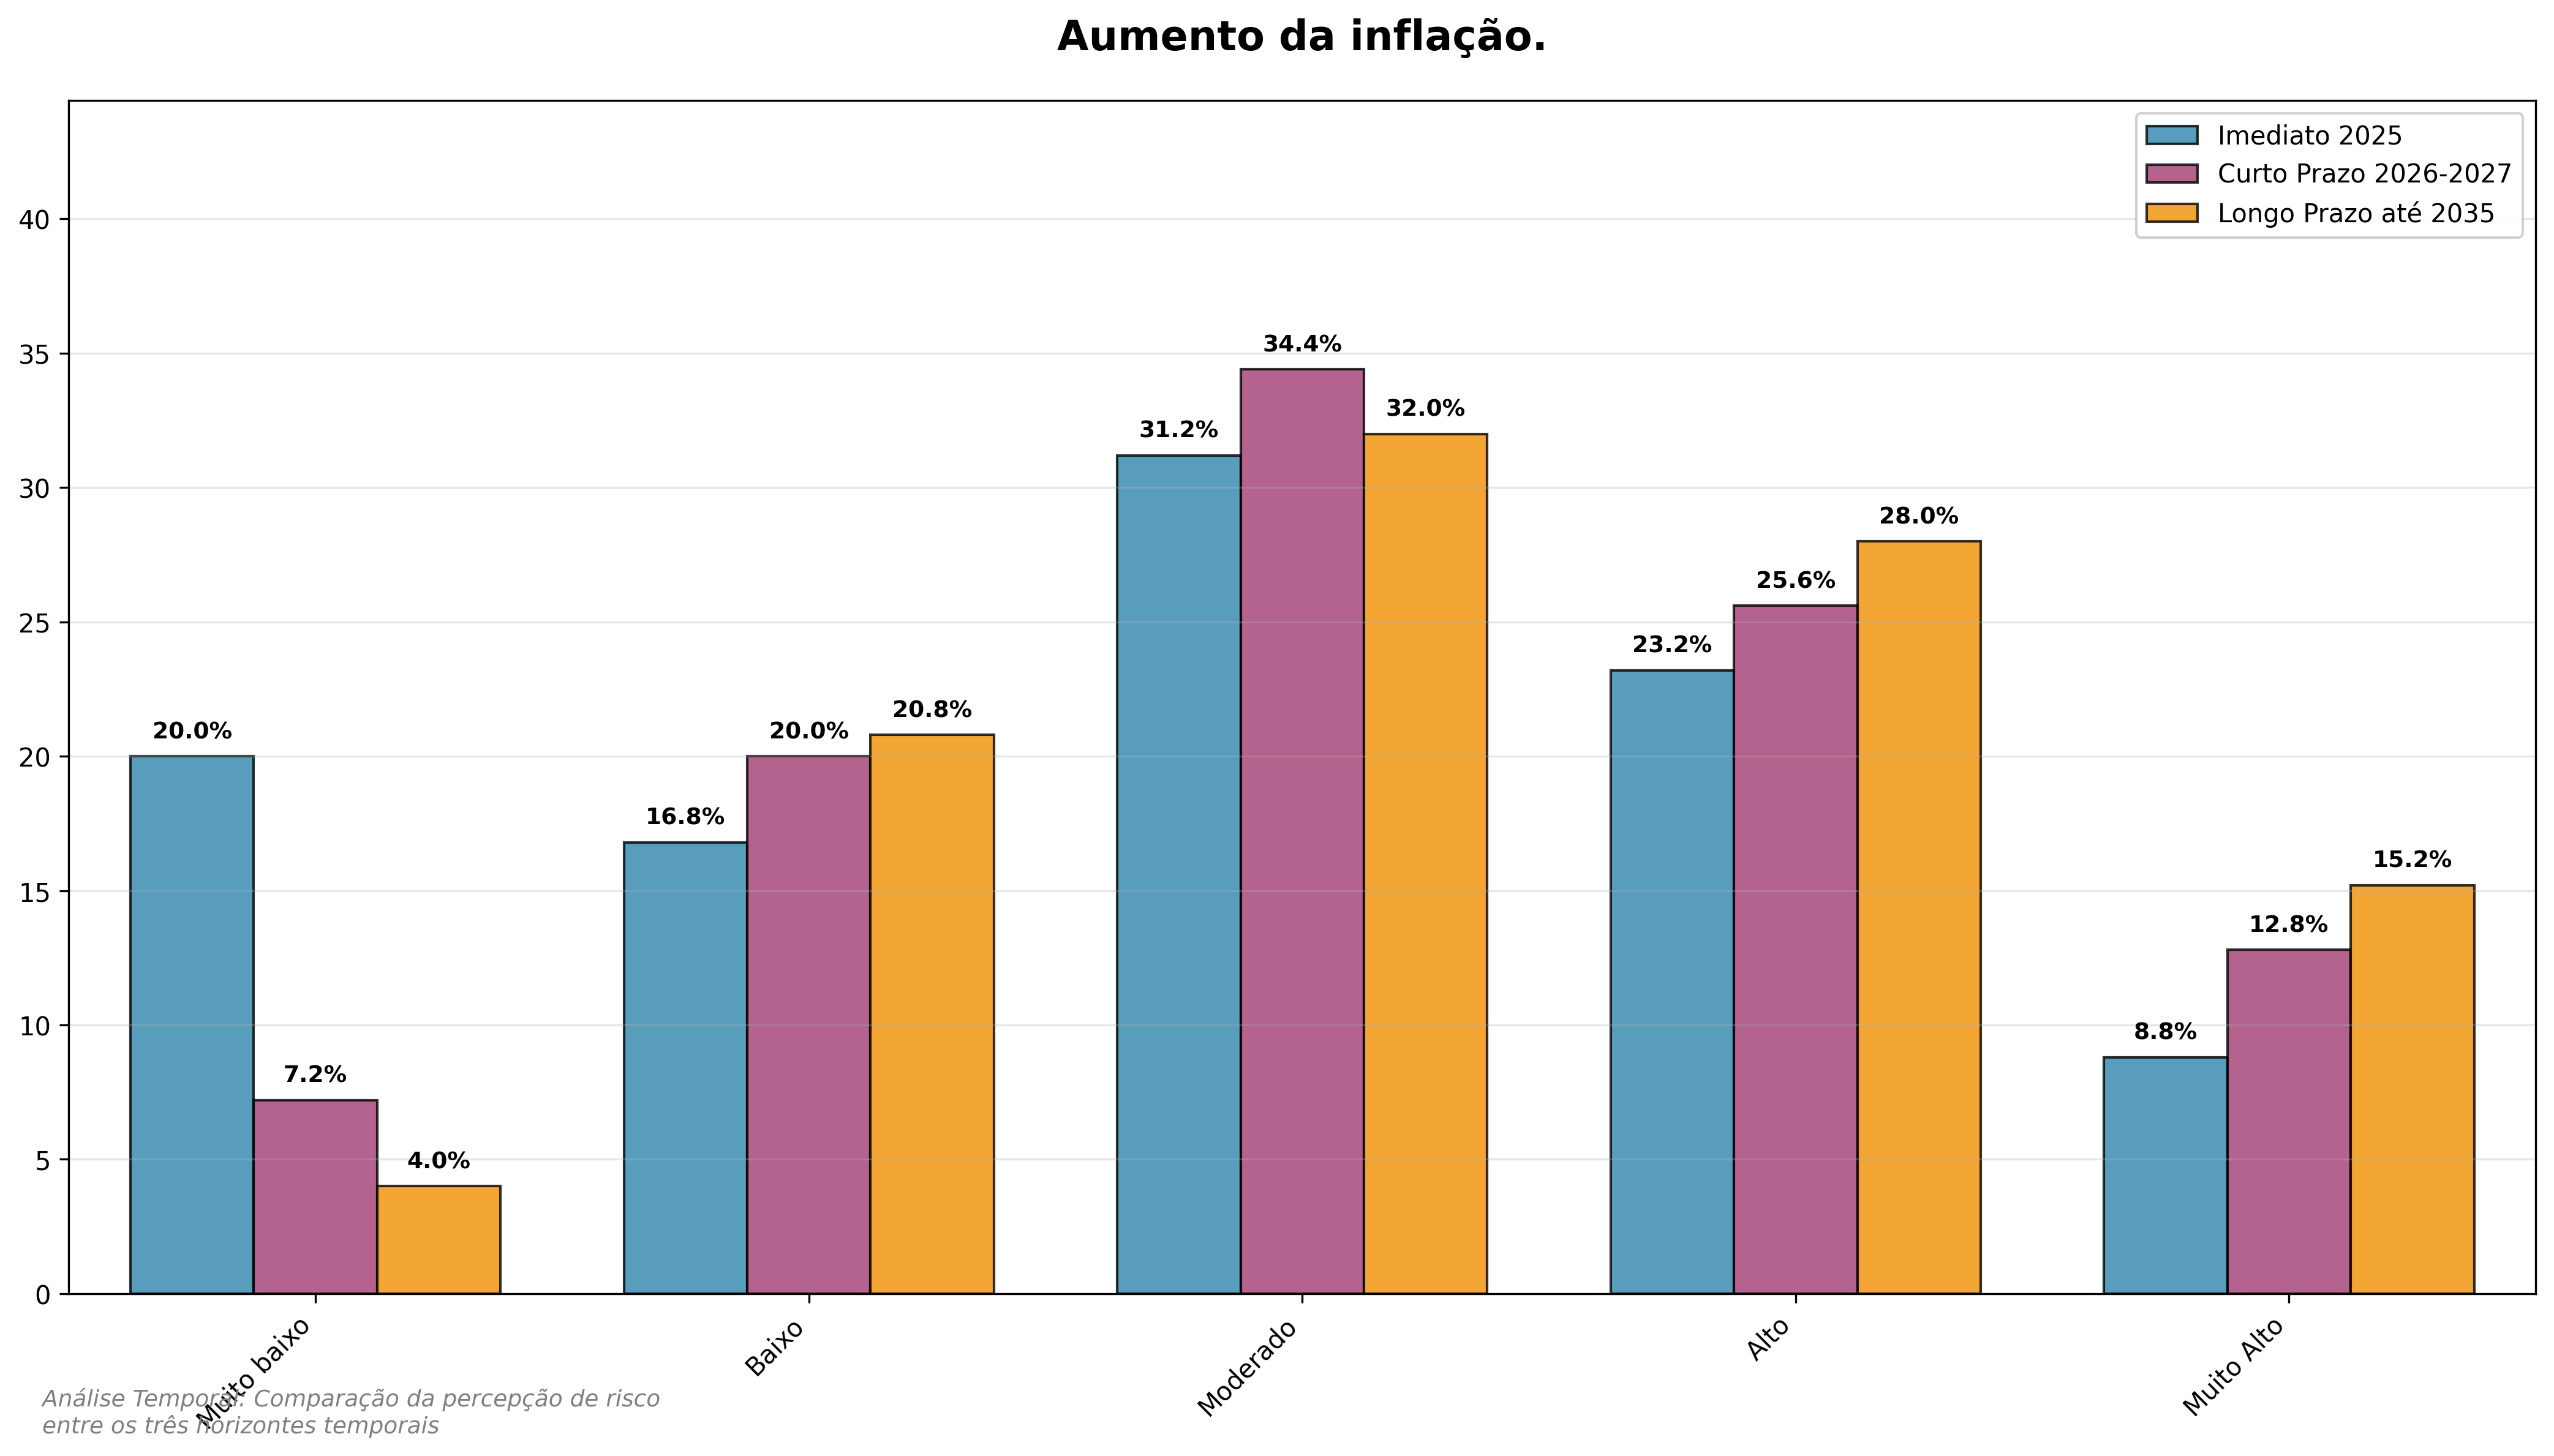
\includegraphics[keepaspectratio]{assets/economicos/grafico_agrupado_1_10_temporal.png}}

\begin{tcolorbox}[enhanced jigsaw, titlerule=0mm, colback=white, title=\textcolor{quarto-callout-tip-color}{\faLightbulb}\hspace{0.5em}{Destaques}, opacityback=0, colbacktitle=quarto-callout-tip-color!10!white, leftrule=.75mm, left=2mm, colframe=quarto-callout-tip-color-frame, bottomrule=.15mm, bottomtitle=1mm, breakable, toprule=.15mm, toptitle=1mm, opacitybacktitle=0.6, arc=.35mm, coltitle=black, rightrule=.15mm]

\textbf{Imediato (2025)}: Mediana 3.0, 32\% em risco alto

\textbf{Curto Prazo (2026-2027)}: Mediana 3.0, 38\% em risco alto

\textbf{Longo Prazo (até 2035)}: Mediana 3.0, 43\% em risco alto

\begin{itemize}
\tightlist
\item
  \textbf{Tendência}: Percepção de risco relativamente estável ao longo
  do tempo. \textbf{Aumento da inflação. {[}Imediato (2025){]}}
\end{itemize}

Risco que depende da atuação das autoridades monetárias do país.
Felizmente, ela tem sido controlada, um preço a se pagar pelas altas
taxas de juros praticadas. Não obstante, pode-se ter aumentos fora da
média para insumos importantes para as atividades portuárias. Controle e
ações remediativas são imperativas.

\end{tcolorbox}

\subsection{Dificuldades de financiamento e obtenção de recursos
financeiros para
investimento}\label{dificuldades-de-financiamento-e-obtenuxe7uxe3o-de-recursos-financeiros-para-investimento}

O gr?fico a seguir apresenta a evolu??o temporal do risco Dificuldades
de financiamento e obtenção de recursos financeiros para investimento.
\pandocbounded{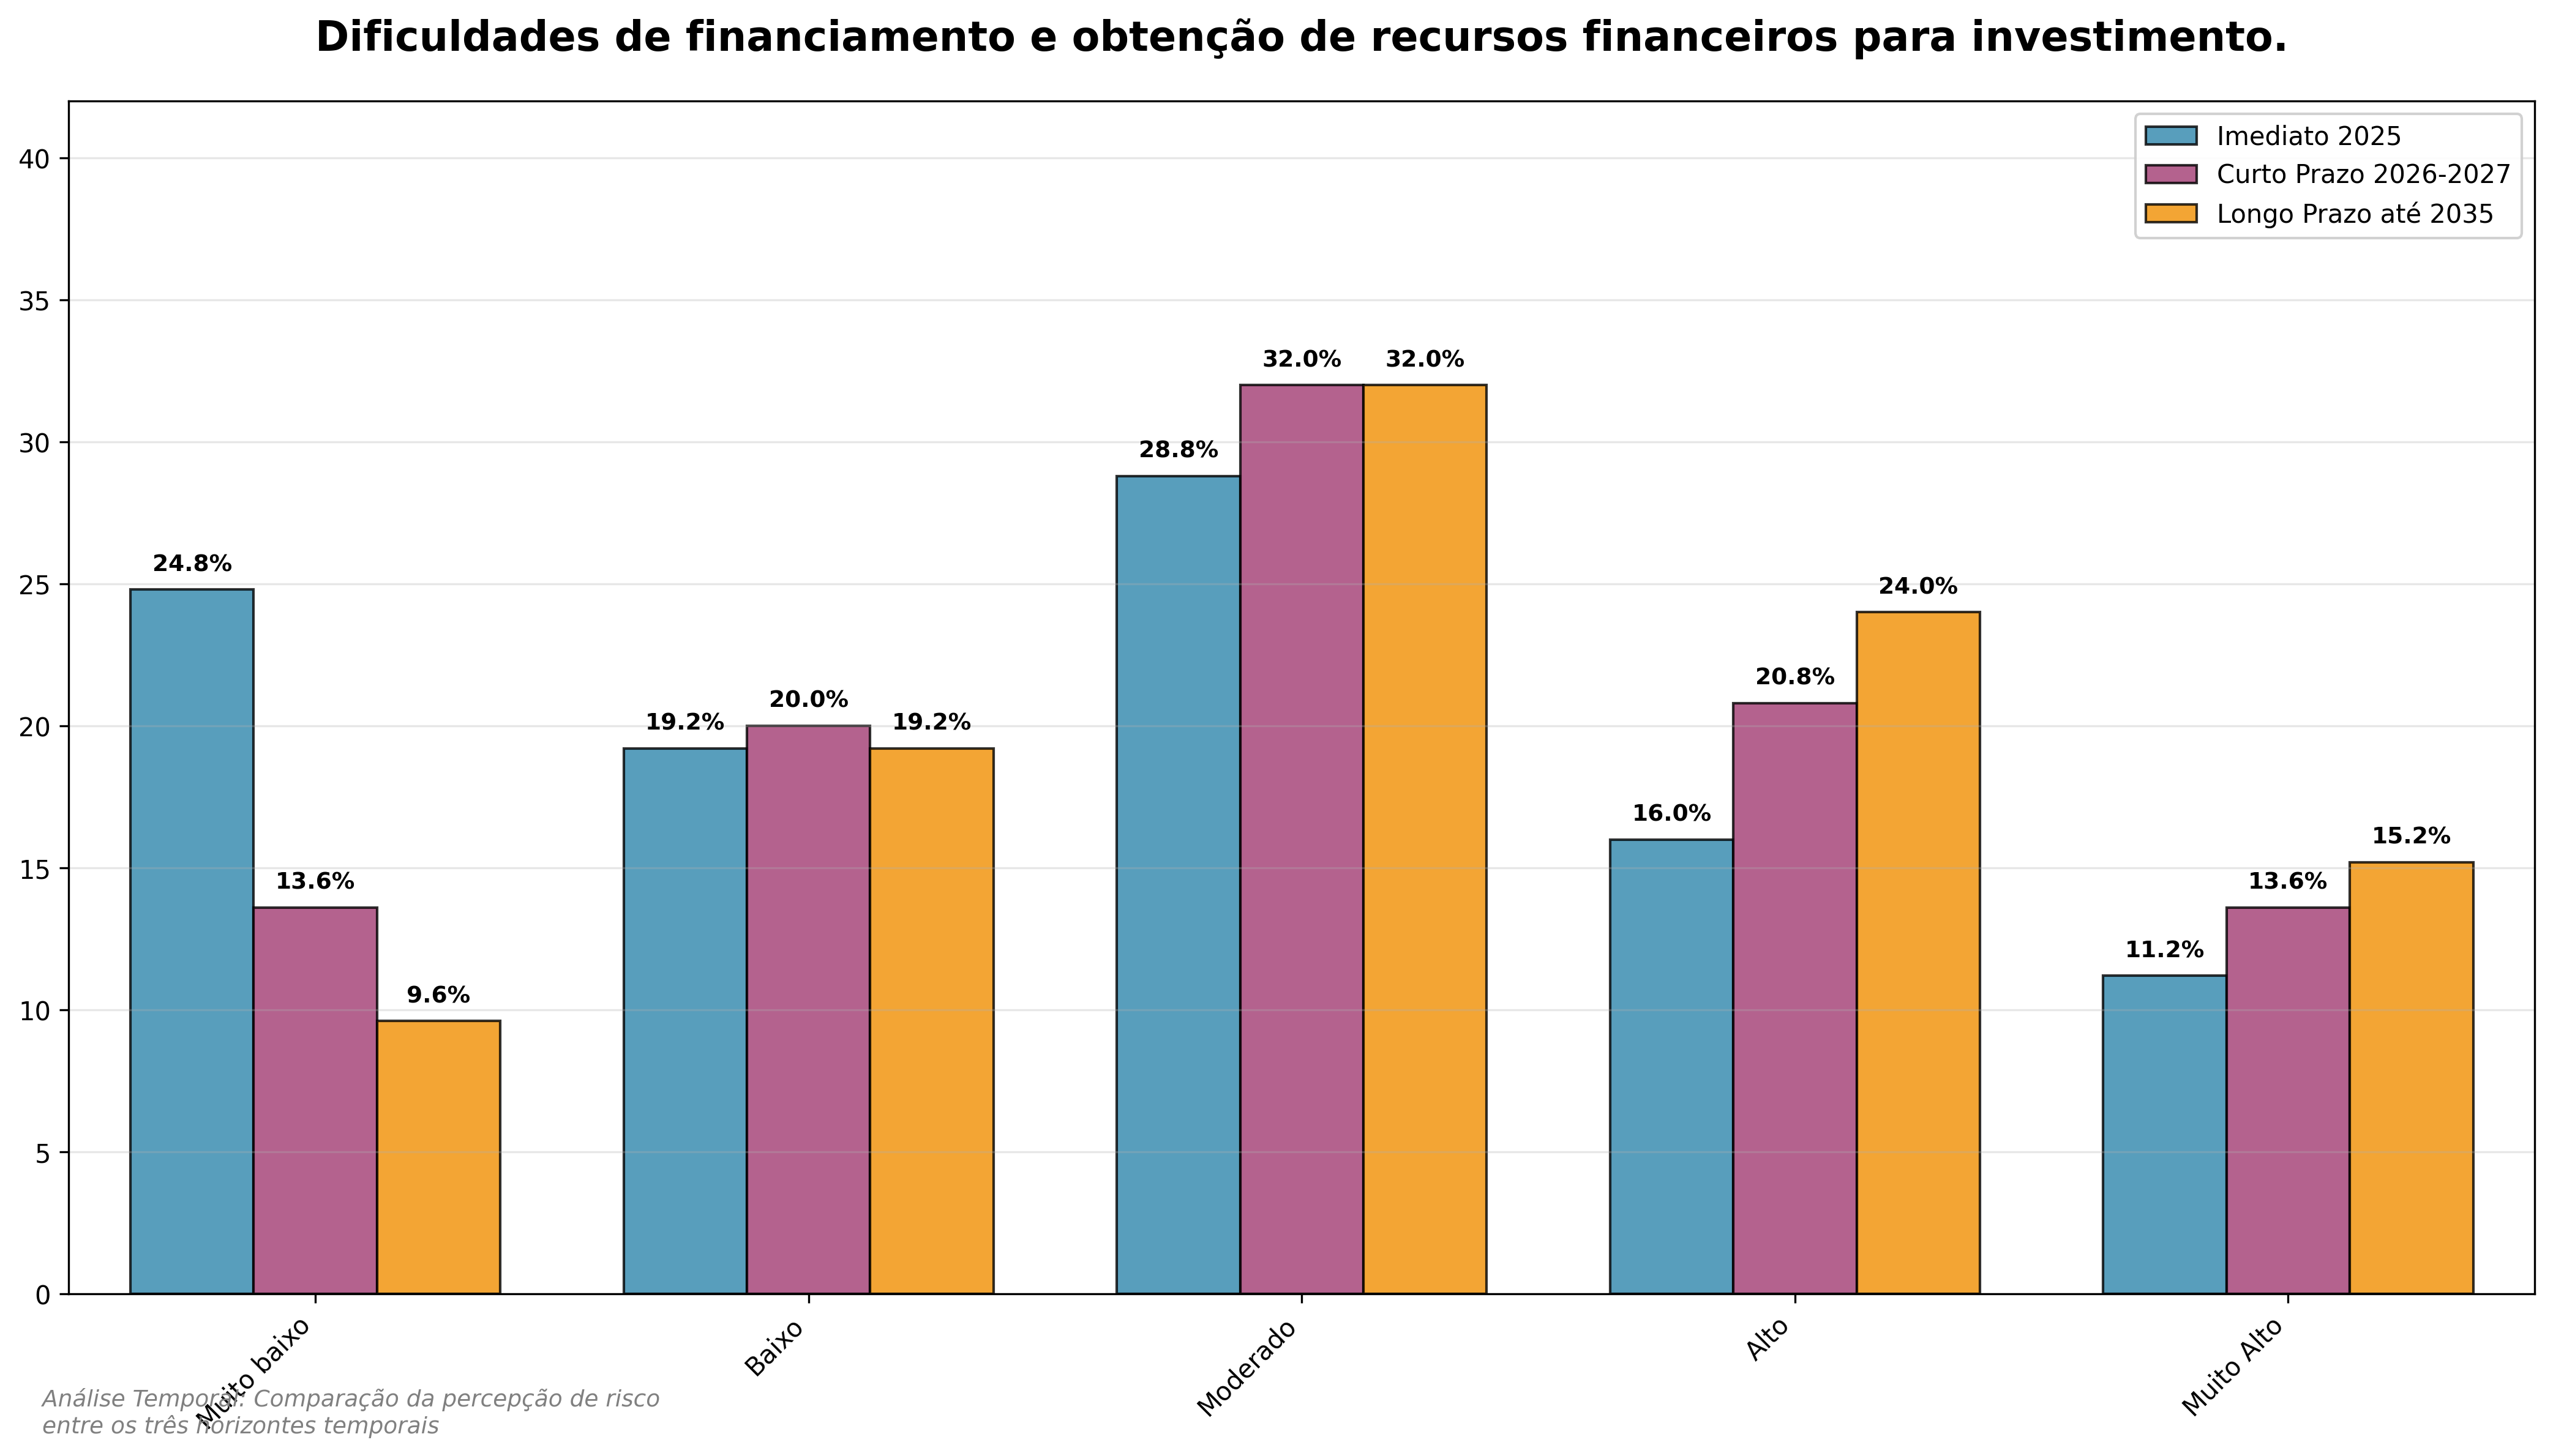
\includegraphics[keepaspectratio]{assets/economicos/grafico_agrupado_1_11_temporal.png}}

\begin{tcolorbox}[enhanced jigsaw, titlerule=0mm, colback=white, title=\textcolor{quarto-callout-tip-color}{\faLightbulb}\hspace{0.5em}{Destaques}, opacityback=0, colbacktitle=quarto-callout-tip-color!10!white, leftrule=.75mm, left=2mm, colframe=quarto-callout-tip-color-frame, bottomrule=.15mm, bottomtitle=1mm, breakable, toprule=.15mm, toptitle=1mm, opacitybacktitle=0.6, arc=.35mm, coltitle=black, rightrule=.15mm]

\textbf{Imediato (2025)}: Mediana 3.0, 27\% em risco alto

\textbf{Curto Prazo (2026-2027)}: Mediana 3.0, 34\% em risco alto

\textbf{Longo Prazo (até 2035)}: Mediana 3.0, 39\% em risco alto

\begin{itemize}
\tightlist
\item
  \textbf{Tendência}: Percepção de risco relativamente estável ao longo
  do tempo. \textbf{Dificuldades de financiamento e obtenção de recursos
  financeiros para investimento. {[}Imediato (2025){]}}
\end{itemize}

O financiamento depende das condições de mercado, das condições do
empreendimento a ser financiado e da organização que vai tomar o encargo
financeiro. É condição natural da atividade que envolve volumes
expressivos de recursos a movimentar.

\end{tcolorbox}

\subsection{Riscos reputacionais}\label{riscos-reputacionais}

O gr?fico a seguir apresenta a evolu??o temporal do risco Riscos
reputacionais.
\pandocbounded{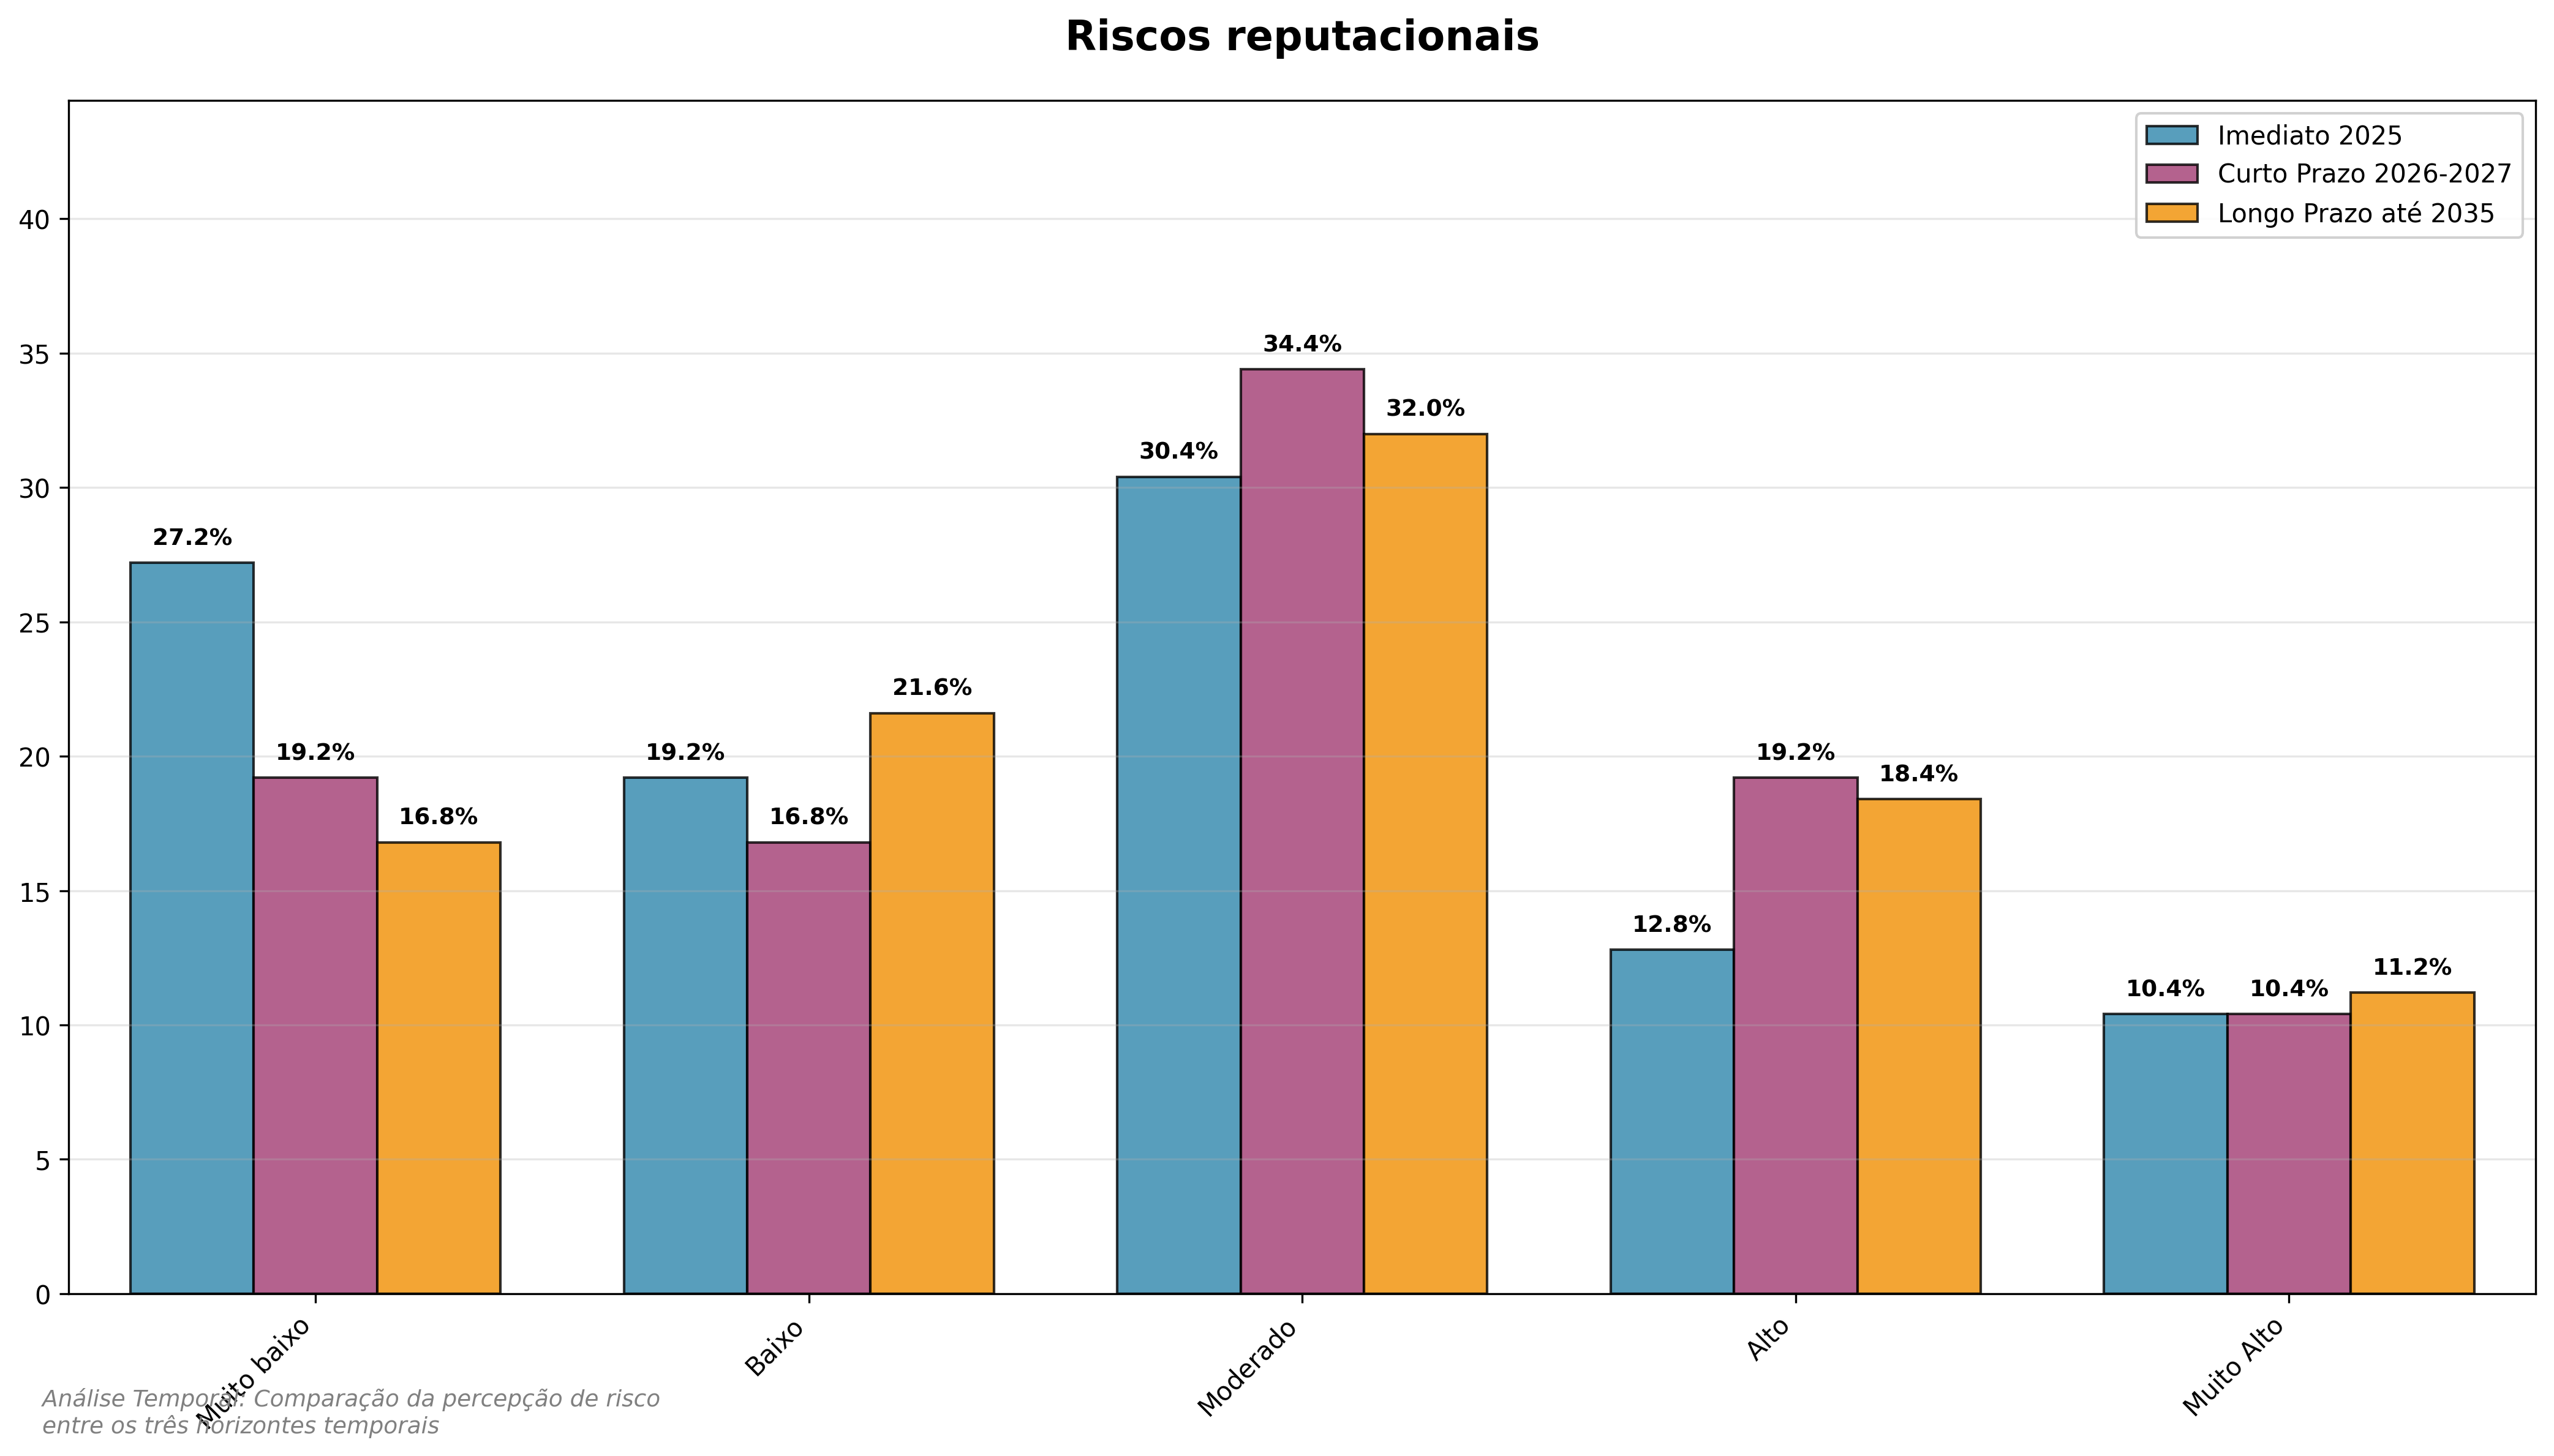
\includegraphics[keepaspectratio]{assets/economicos/grafico_agrupado_1_12_temporal.png}}

\begin{tcolorbox}[enhanced jigsaw, titlerule=0mm, colback=white, title=\textcolor{quarto-callout-tip-color}{\faLightbulb}\hspace{0.5em}{Destaques}, opacityback=0, colbacktitle=quarto-callout-tip-color!10!white, leftrule=.75mm, left=2mm, colframe=quarto-callout-tip-color-frame, bottomrule=.15mm, bottomtitle=1mm, breakable, toprule=.15mm, toptitle=1mm, opacitybacktitle=0.6, arc=.35mm, coltitle=black, rightrule=.15mm]

\textbf{Imediato (2025)}: Mediana 3.0, 23\% em risco alto

\textbf{Curto Prazo (2026-2027)}: Mediana 3.0, 30\% em risco alto

\textbf{Longo Prazo (até 2035)}: Mediana 3.0, 30\% em risco alto

\begin{itemize}
\tightlist
\item
  \textbf{Tendência}: Percepção estável, com leve elevação ao passar
  para o curto prazo. \textbf{Riscos reputacionais. Referem-se à
  possibilidade de danos à reputação de uma organização devido a
  eventos, comportamentos, práticas ou percepções negativas.}
\end{itemize}

Mesmo em um ambiente operacional com controles consolidados, incidentes
comunicacionais e falhas de governança rapidamente repercutem sobre a
legitimidade dos terminais. A estabilidade das medianas evidencia que o
risco é estrutural: não cresce de forma acelerada, mas exige vigilância
permanente, protocolos de relacionamento com stakeholders e respostas
coordenadas para preservar a confiança na operação portuária.

\end{tcolorbox}

\subsection{Risco de competitividade
portuária}\label{risco-de-competitividade-portuuxe1ria}

O gr?fico a seguir apresenta a evolu??o temporal do risco Risco de
competitividade portuária.
\pandocbounded{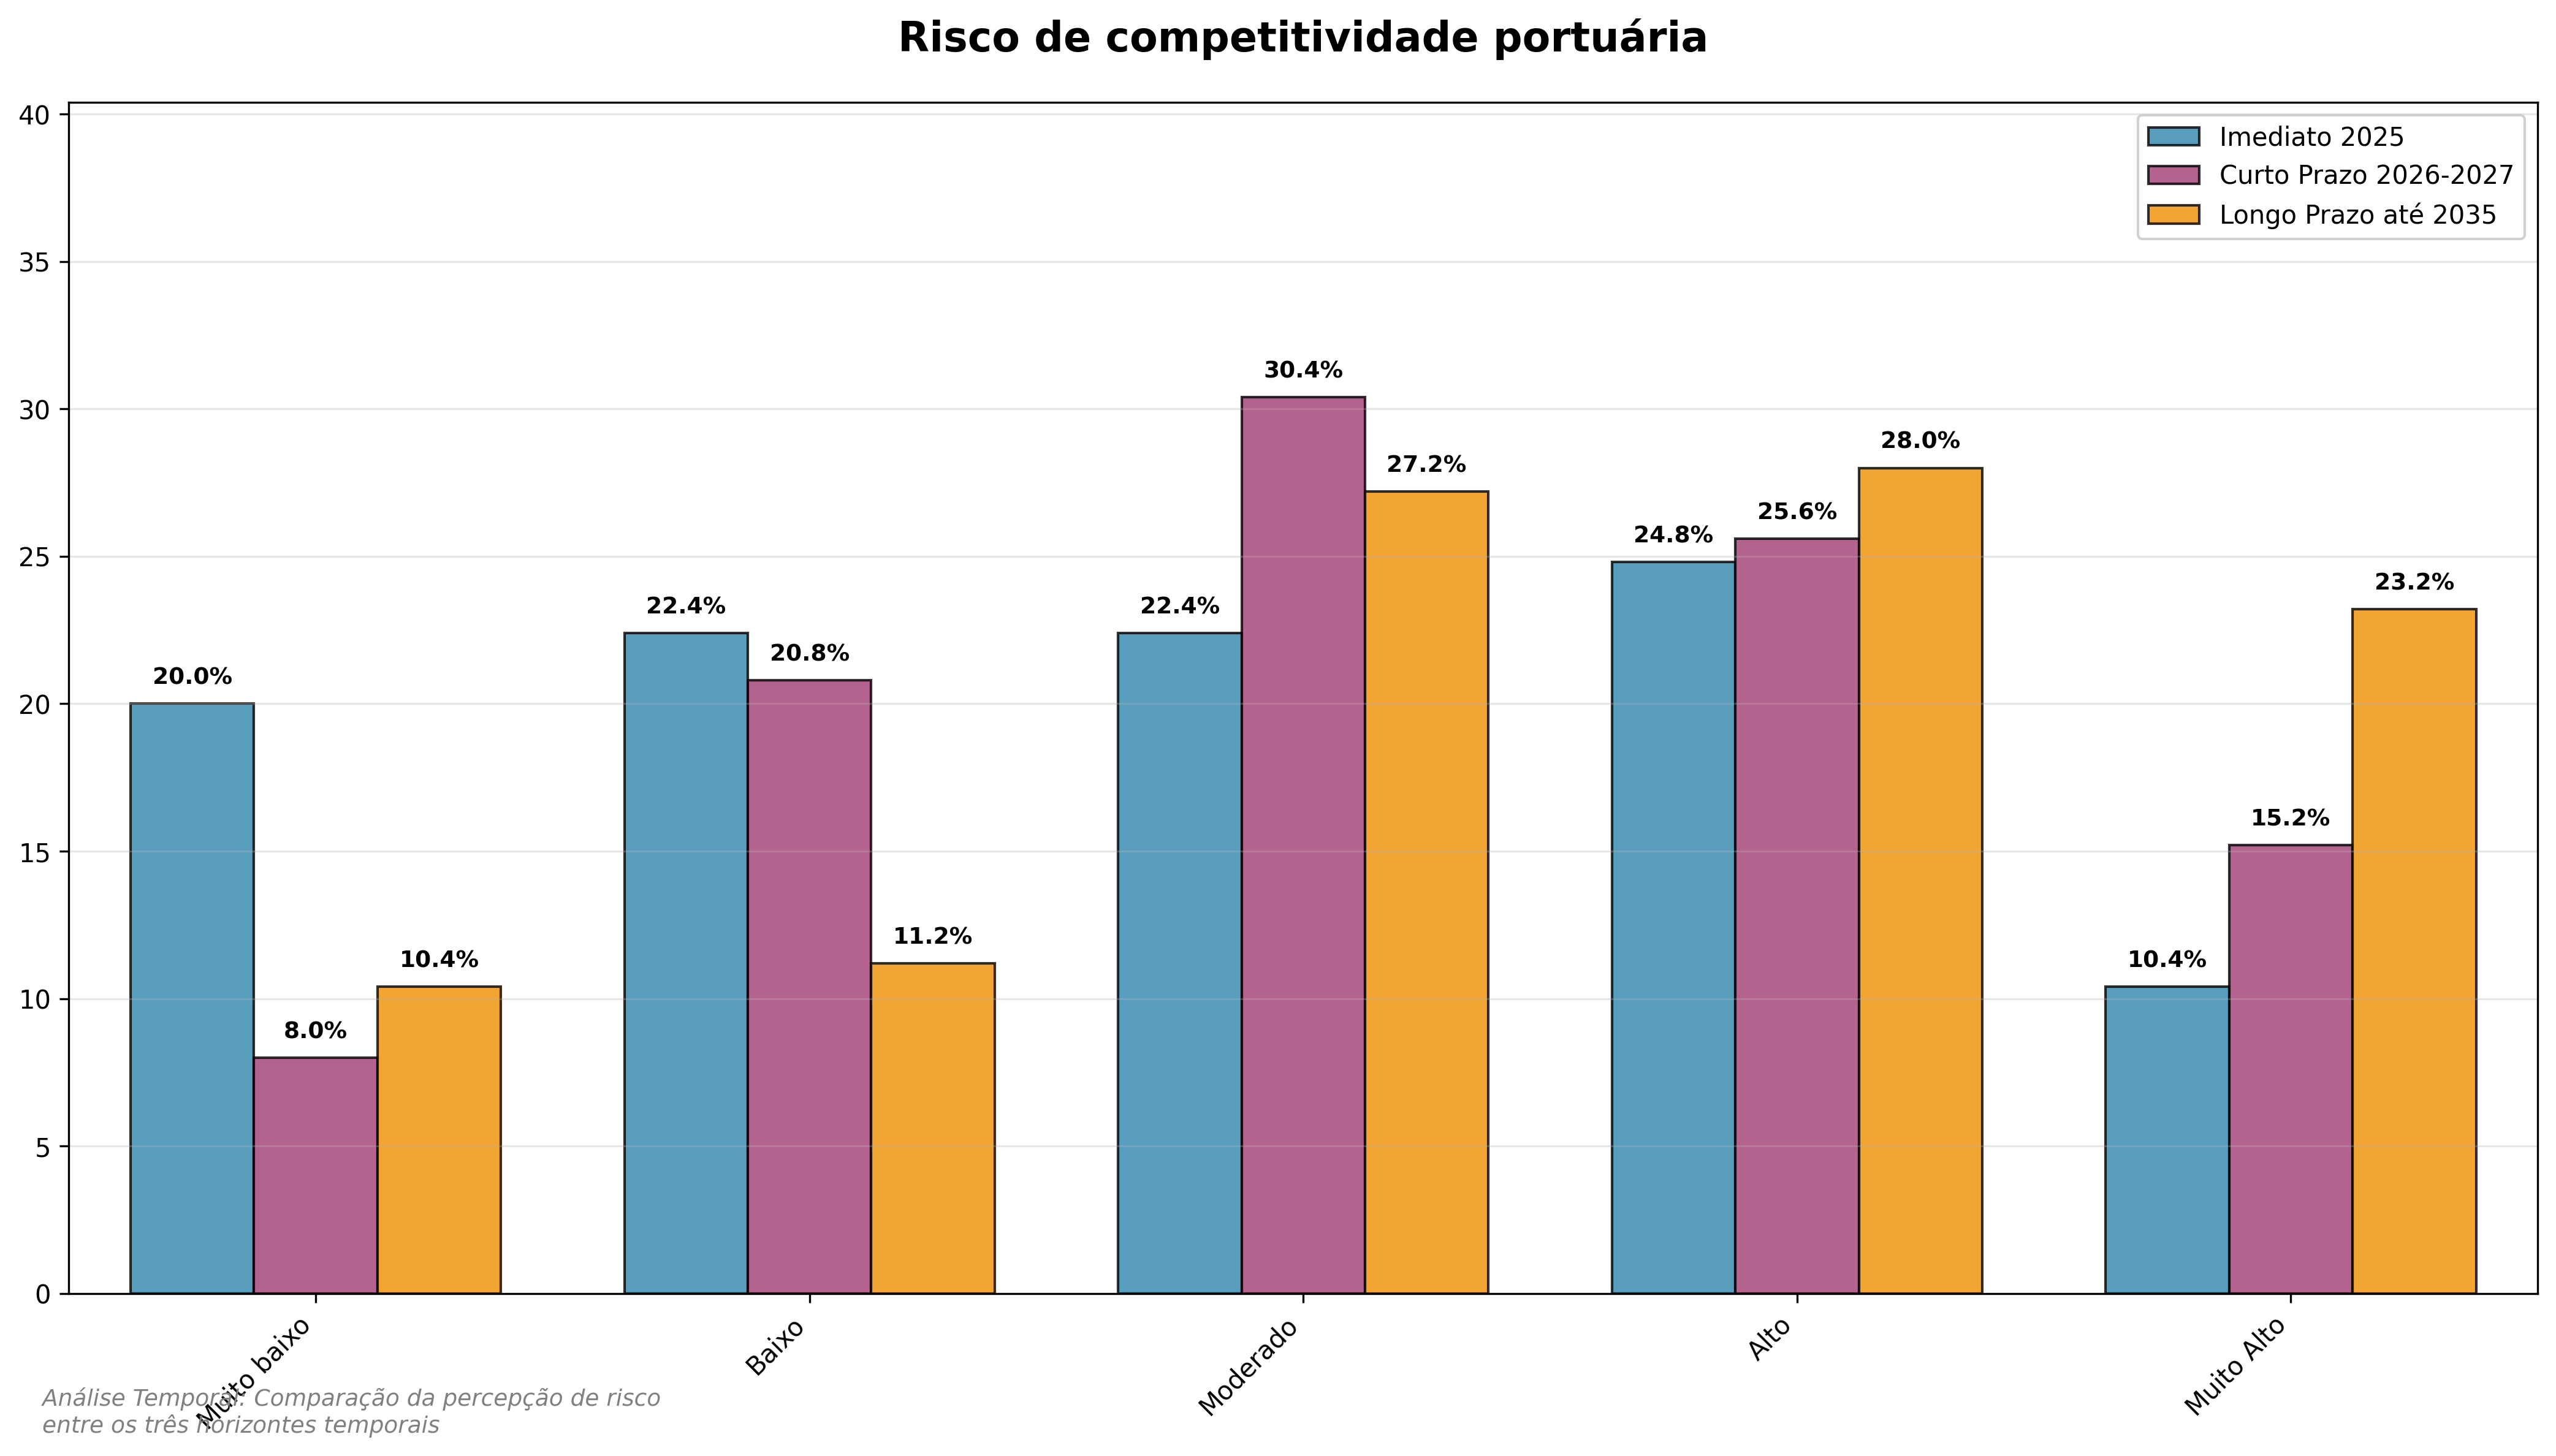
\includegraphics[keepaspectratio]{assets/economicos/grafico_agrupado_1_13_temporal.png}}

\begin{tcolorbox}[enhanced jigsaw, titlerule=0mm, colback=white, title=\textcolor{quarto-callout-tip-color}{\faLightbulb}\hspace{0.5em}{Destaques}, opacityback=0, colbacktitle=quarto-callout-tip-color!10!white, leftrule=.75mm, left=2mm, colframe=quarto-callout-tip-color-frame, bottomrule=.15mm, bottomtitle=1mm, breakable, toprule=.15mm, toptitle=1mm, opacitybacktitle=0.6, arc=.35mm, coltitle=black, rightrule=.15mm]

\textbf{Imediato (2025)}: Mediana 3.0, 35\% em risco alto

\textbf{Curto Prazo (2026-2027)}: Mediana 3.0, 41\% em risco alto

\textbf{Longo Prazo (até 2035)}: Mediana 4.0, 51\% em risco alto

\begin{itemize}
\tightlist
\item
  \textbf{Tendência}: Escalada contínua, culminando em patamar crítico
  no longo prazo. \textbf{Risco de competitividade portuária. Riscos
  relacionados à concorrência entre portos referem-se às ameaças e
  desafios enfrentados diante de players que oferecem serviços de custo
  menor ou maior eficiência operacional.}
\end{itemize}

A pressão competitiva aparece de forma moderada no imediato, mas cresce
rapidamente à medida que novos investimentos e corredores logísticos
surgem. O salto da mediana para 4.0 no horizonte de 2035 indica que os
portos precisarão sustentar produtividade, diferenciação de serviços e
alianças estratégicas de longo prazo para manter posição nos fluxos
globais.

\end{tcolorbox}

\subsection{Aumento de impostos}\label{aumento-de-impostos}

O gr?fico a seguir apresenta a evolu??o temporal do risco Aumento de
impostos.
\pandocbounded{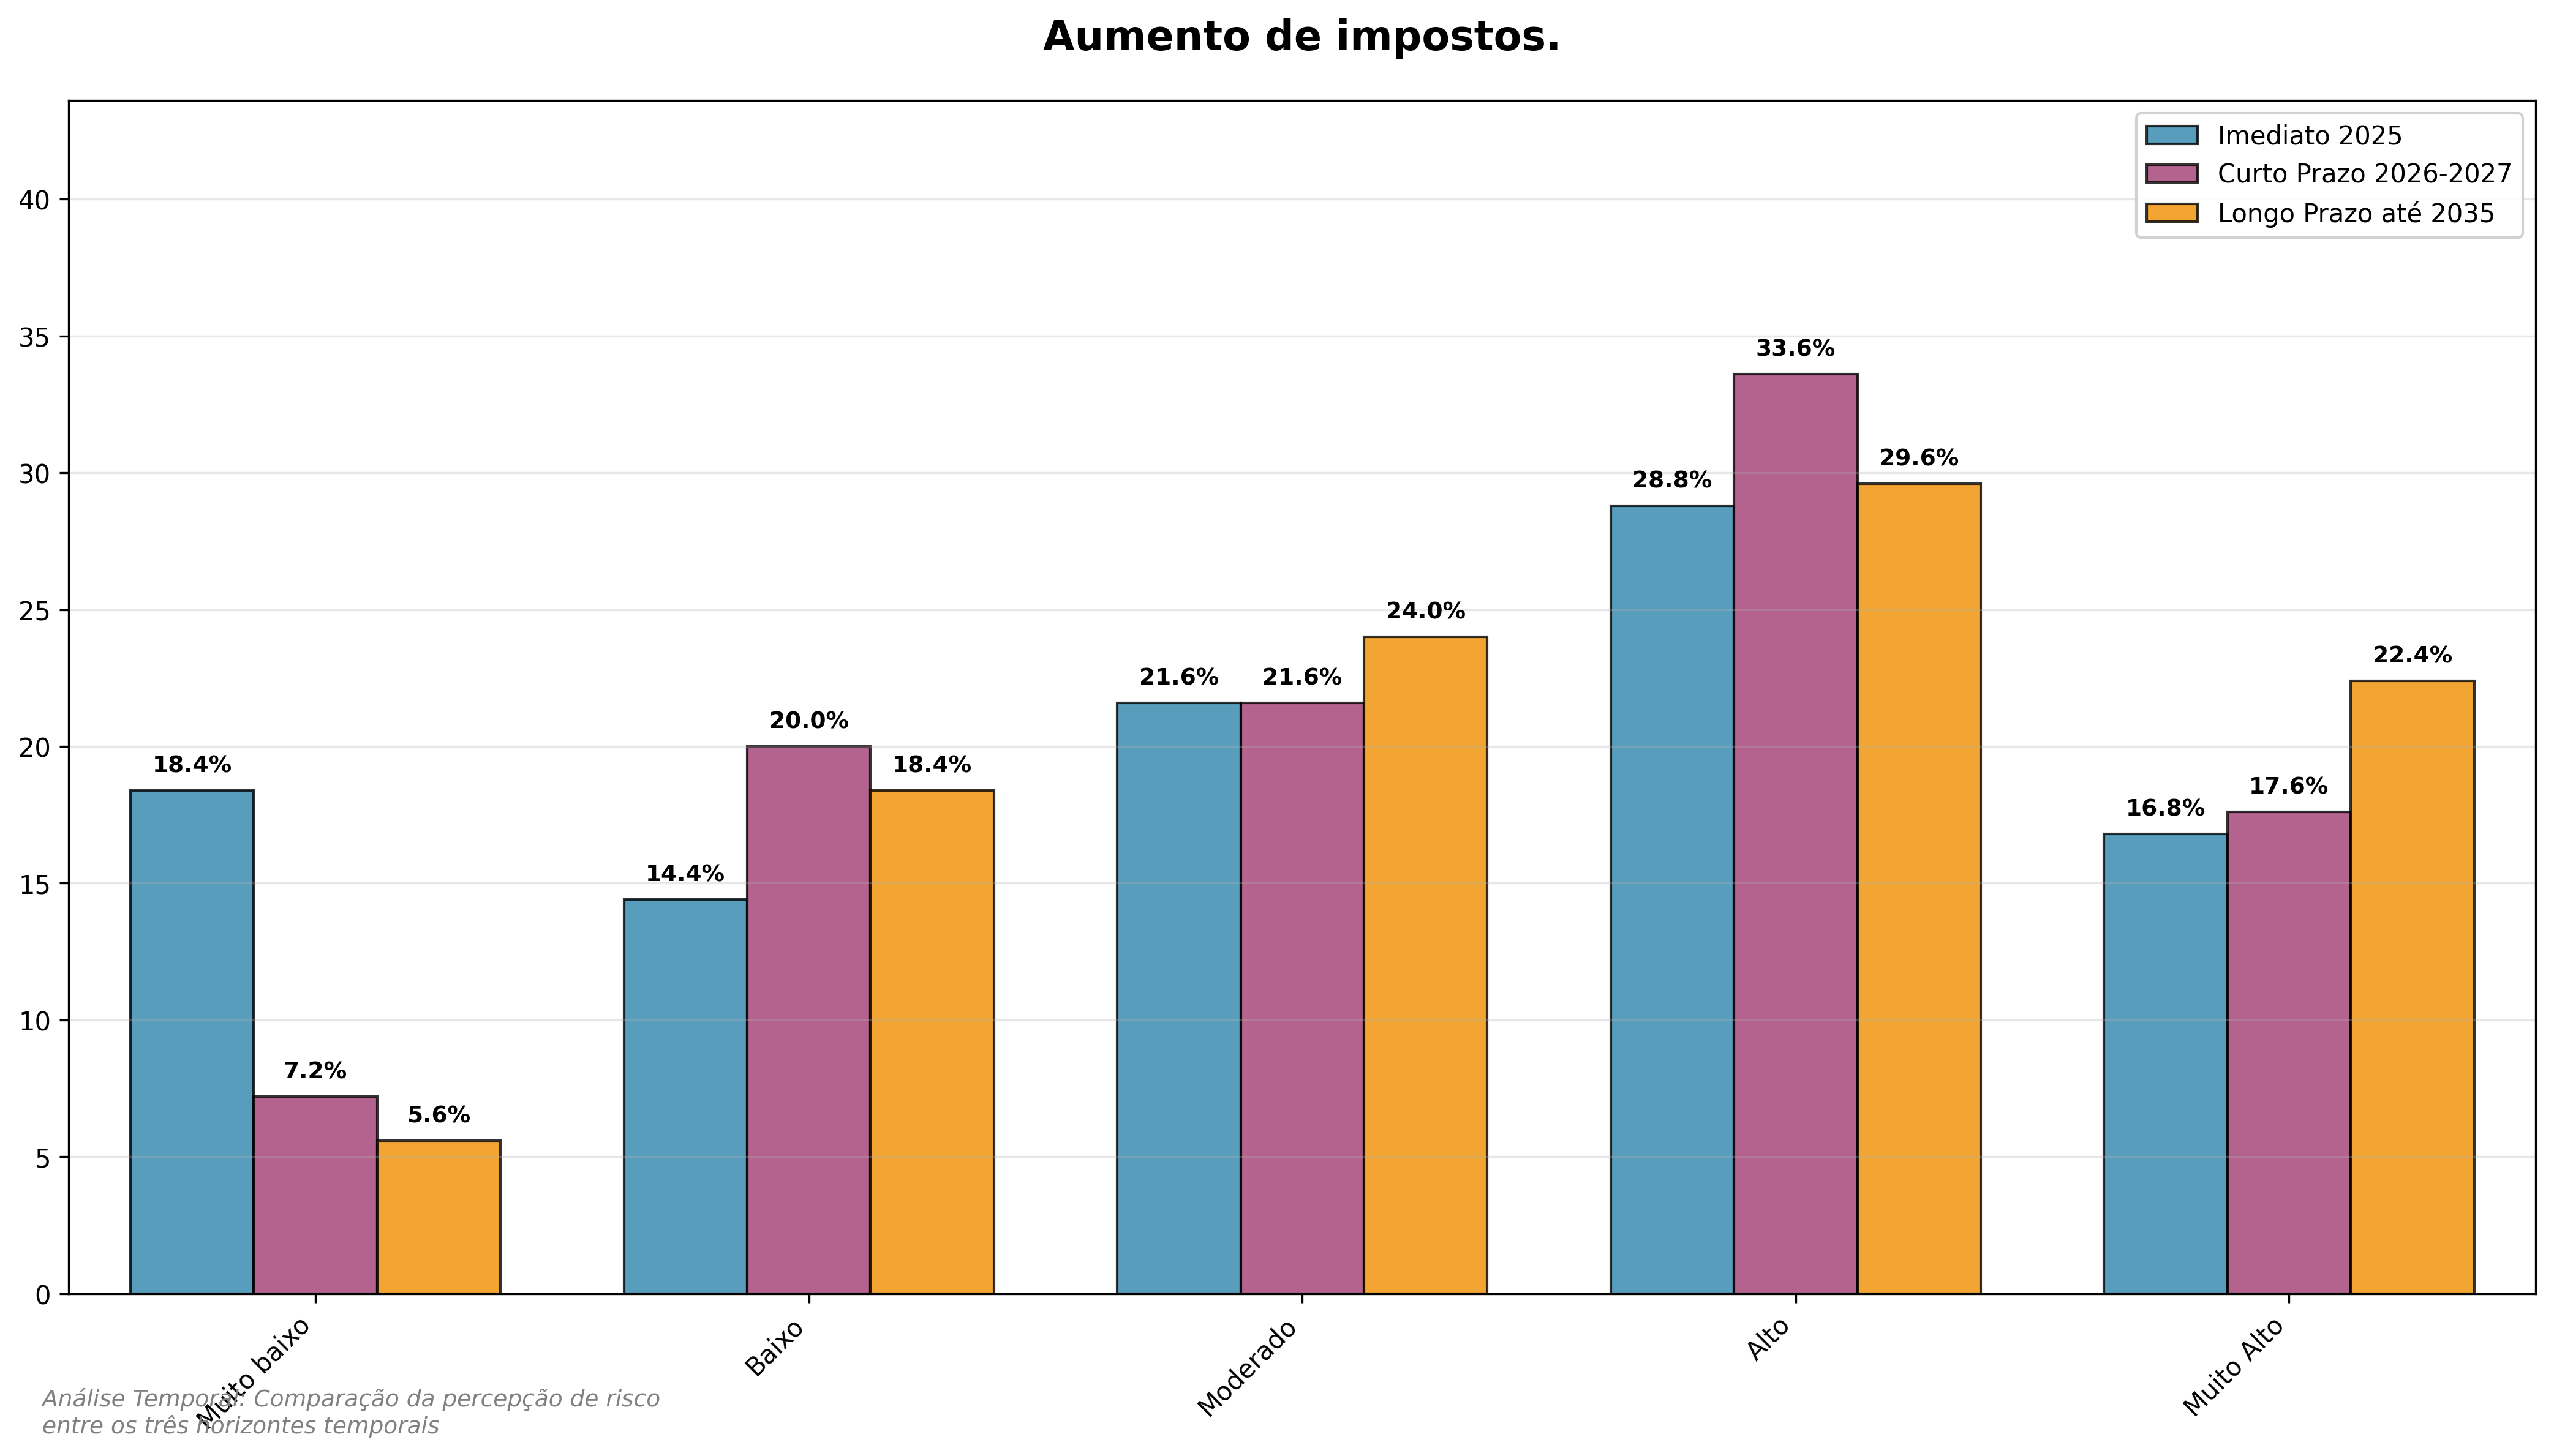
\includegraphics[keepaspectratio]{assets/economicos/grafico_agrupado_1_14_temporal.png}}

\begin{tcolorbox}[enhanced jigsaw, titlerule=0mm, colback=white, title=\textcolor{quarto-callout-tip-color}{\faLightbulb}\hspace{0.5em}{Destaques}, opacityback=0, colbacktitle=quarto-callout-tip-color!10!white, leftrule=.75mm, left=2mm, colframe=quarto-callout-tip-color-frame, bottomrule=.15mm, bottomtitle=1mm, breakable, toprule=.15mm, toptitle=1mm, opacitybacktitle=0.6, arc=.35mm, coltitle=black, rightrule=.15mm]

\textbf{Imediato (2025)}: Mediana 3.0, 46\% em risco alto

\textbf{Curto Prazo (2026-2027)}: Mediana 4.0, 54\% em risco alto

\textbf{Longo Prazo (até 2035)}: Mediana 4.0, 53\% em risco alto

\begin{itemize}
\tightlist
\item
  \textbf{Tendência}: Percepção de risco relativamente estável ao longo
  do tempo. \textbf{Aumento de impostos.}
\end{itemize}

A condição de aumento de impostos tem de ser analisada em relação às
condições de concorrência e à possibilidade de mercado de repassá-los a
clientes e parceiros.

\end{tcolorbox}

\subsection{Instabilidade política}\label{instabilidade-poluxedtica}

O gr?fico a seguir apresenta a evolu??o temporal do risco Instabilidade
política.
\pandocbounded{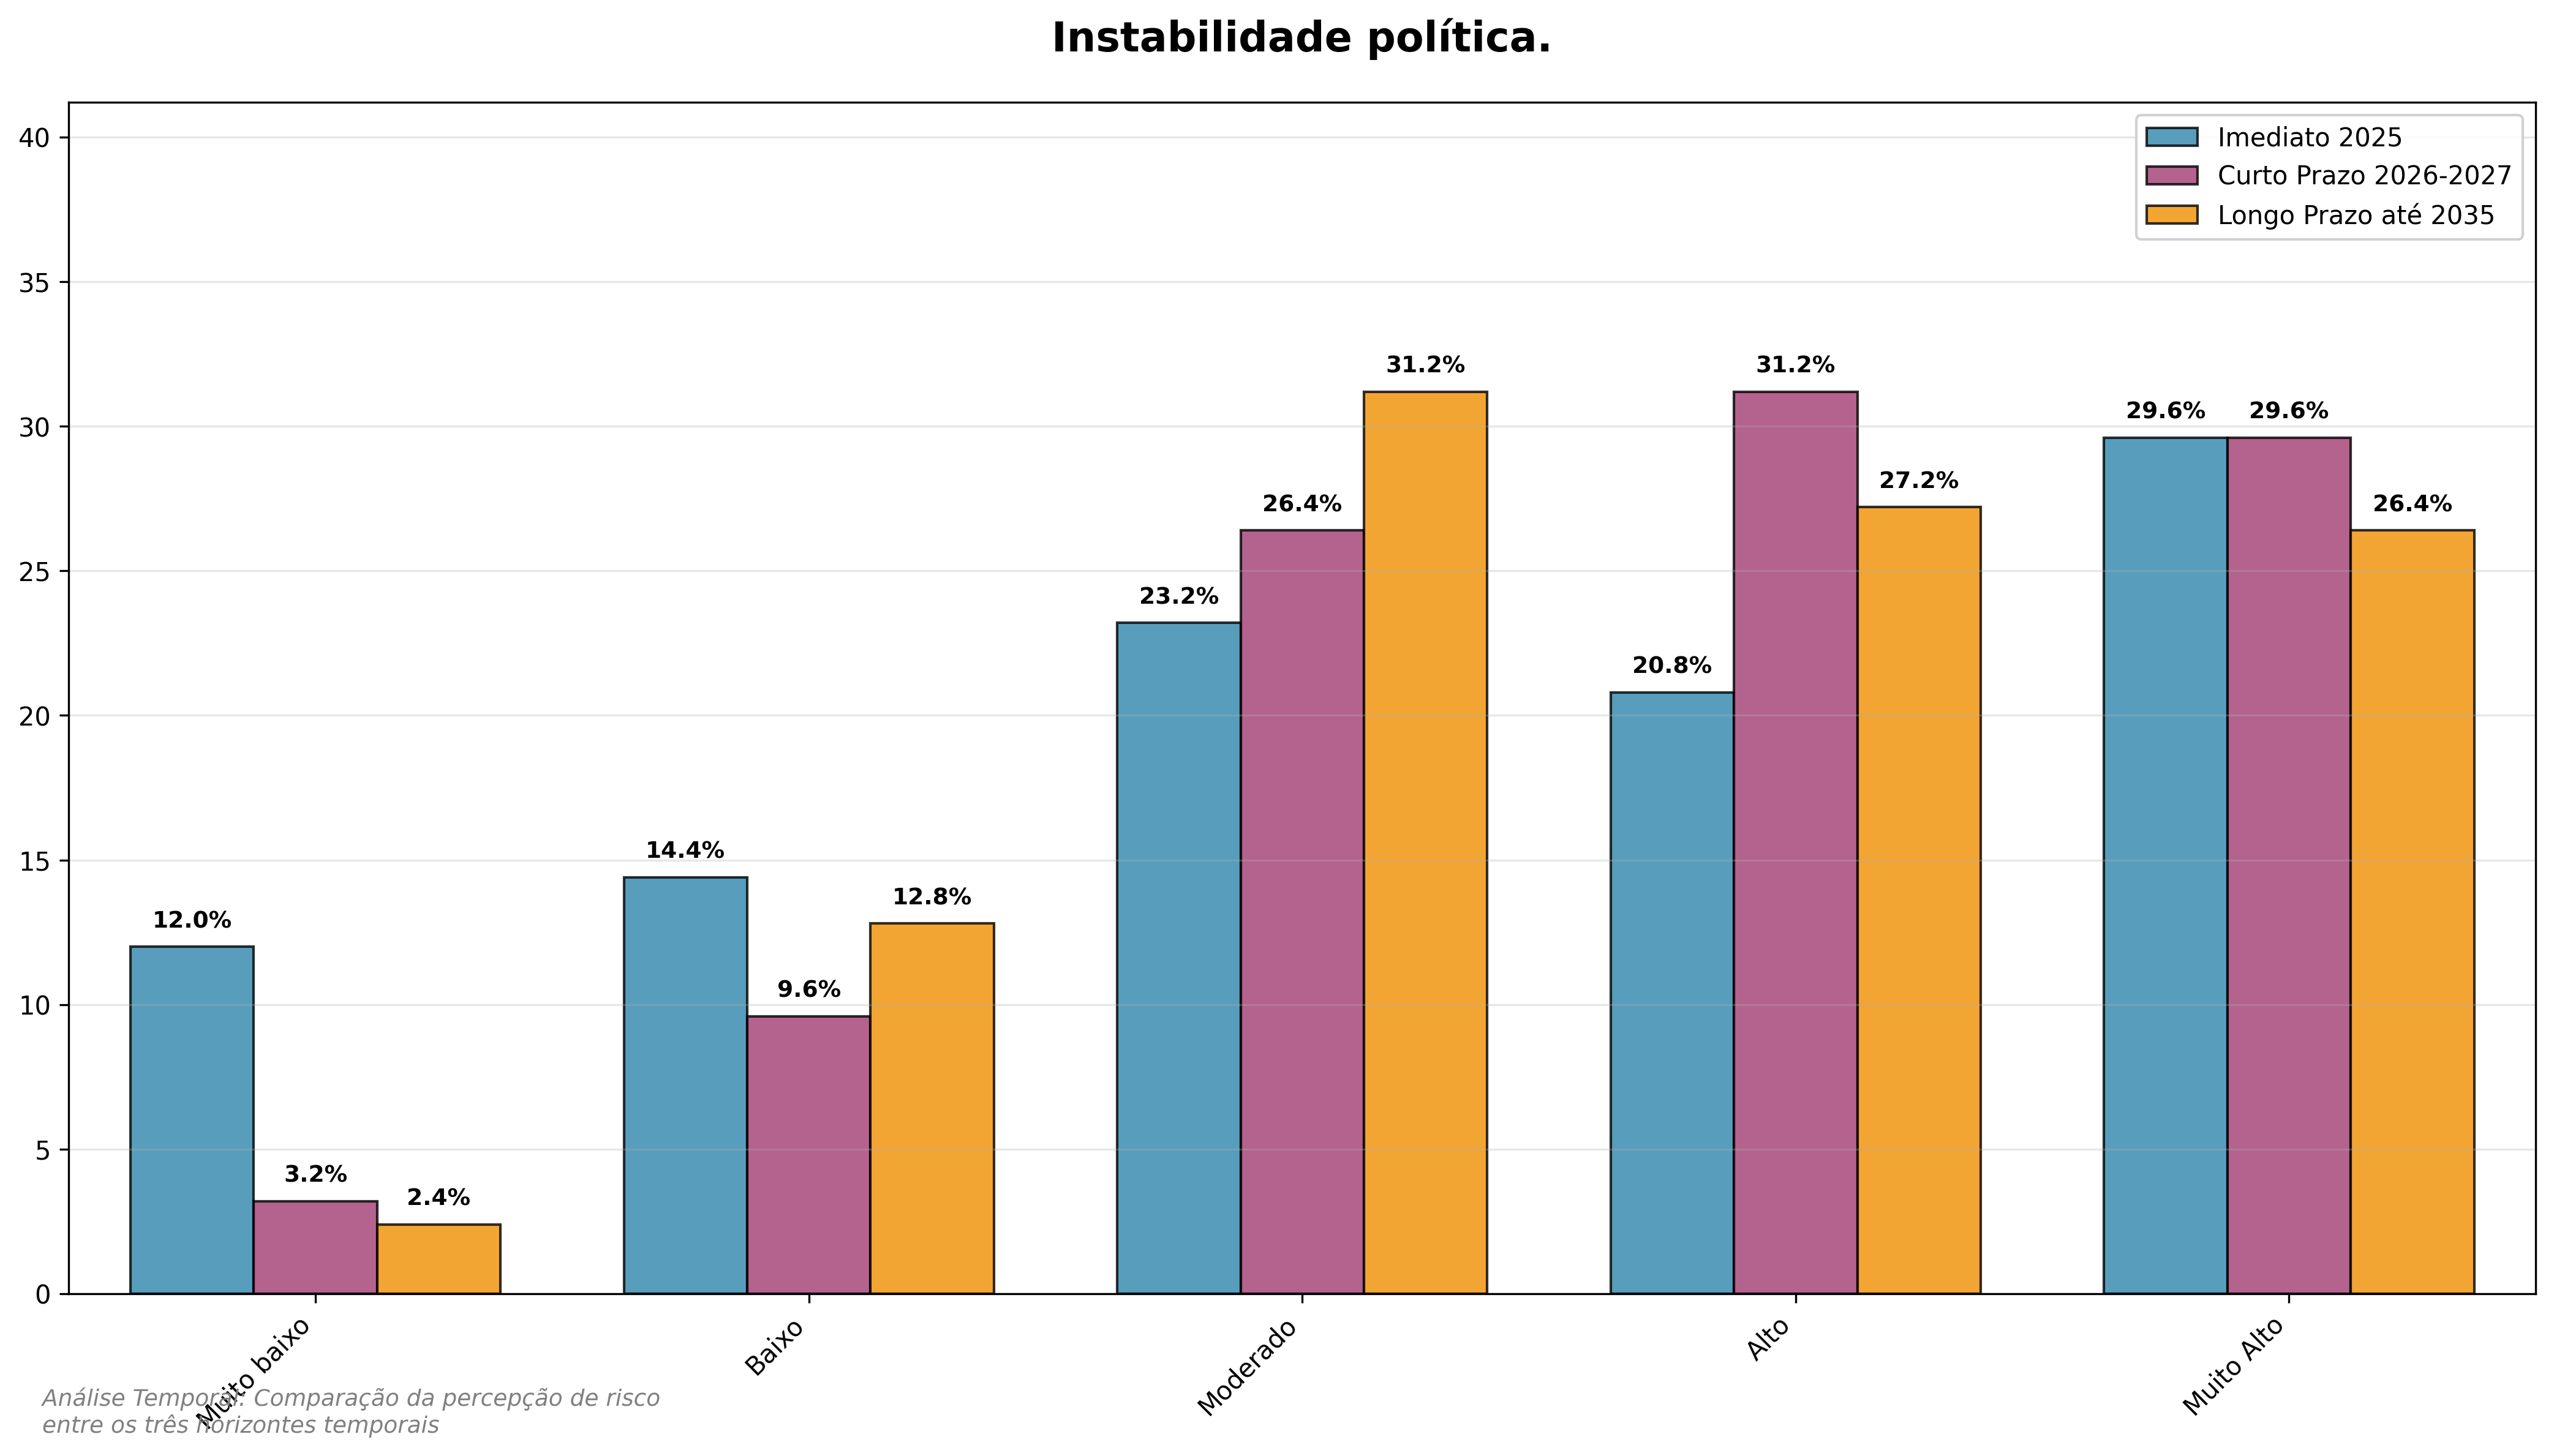
\includegraphics[keepaspectratio]{assets/economicos/grafico_agrupado_1_15_temporal.png}}

\begin{tcolorbox}[enhanced jigsaw, titlerule=0mm, colback=white, title=\textcolor{quarto-callout-tip-color}{\faLightbulb}\hspace{0.5em}{Destaques}, opacityback=0, colbacktitle=quarto-callout-tip-color!10!white, leftrule=.75mm, left=2mm, colframe=quarto-callout-tip-color-frame, bottomrule=.15mm, bottomtitle=1mm, breakable, toprule=.15mm, toptitle=1mm, opacitybacktitle=0.6, arc=.35mm, coltitle=black, rightrule=.15mm]

\textbf{Imediato (2025)}: Mediana 3.0, 25\% em risco alto

\textbf{Curto Prazo (2026-2027)}: Mediana 3.0, 27\% em risco alto

\textbf{Longo Prazo (até 2035)}: Mediana 3.0, 34\% em risco alto

\begin{itemize}
\tightlist
\item
  \textbf{Tendência}: Percepção de risco relativamente estável ao longo
  do tempo. \textbf{Instabilidade política.}
\end{itemize}

Risco estratégico que transcende a esfera operacional e impacta
diretamente a governança e sustentabilidade das operações portuárias.
Decorre da dinâmica democrática e da alternância de poder, especialmente
em portos públicos onde mudanças administrativas podem ocorrer com a
transição de grupos políticos.

\end{tcolorbox}

\subsection{Déficit regulatório}\label{duxe9ficit-regulatuxf3rio}

O gr?fico a seguir apresenta a evolu??o temporal do risco Déficit
regulatório.
\pandocbounded{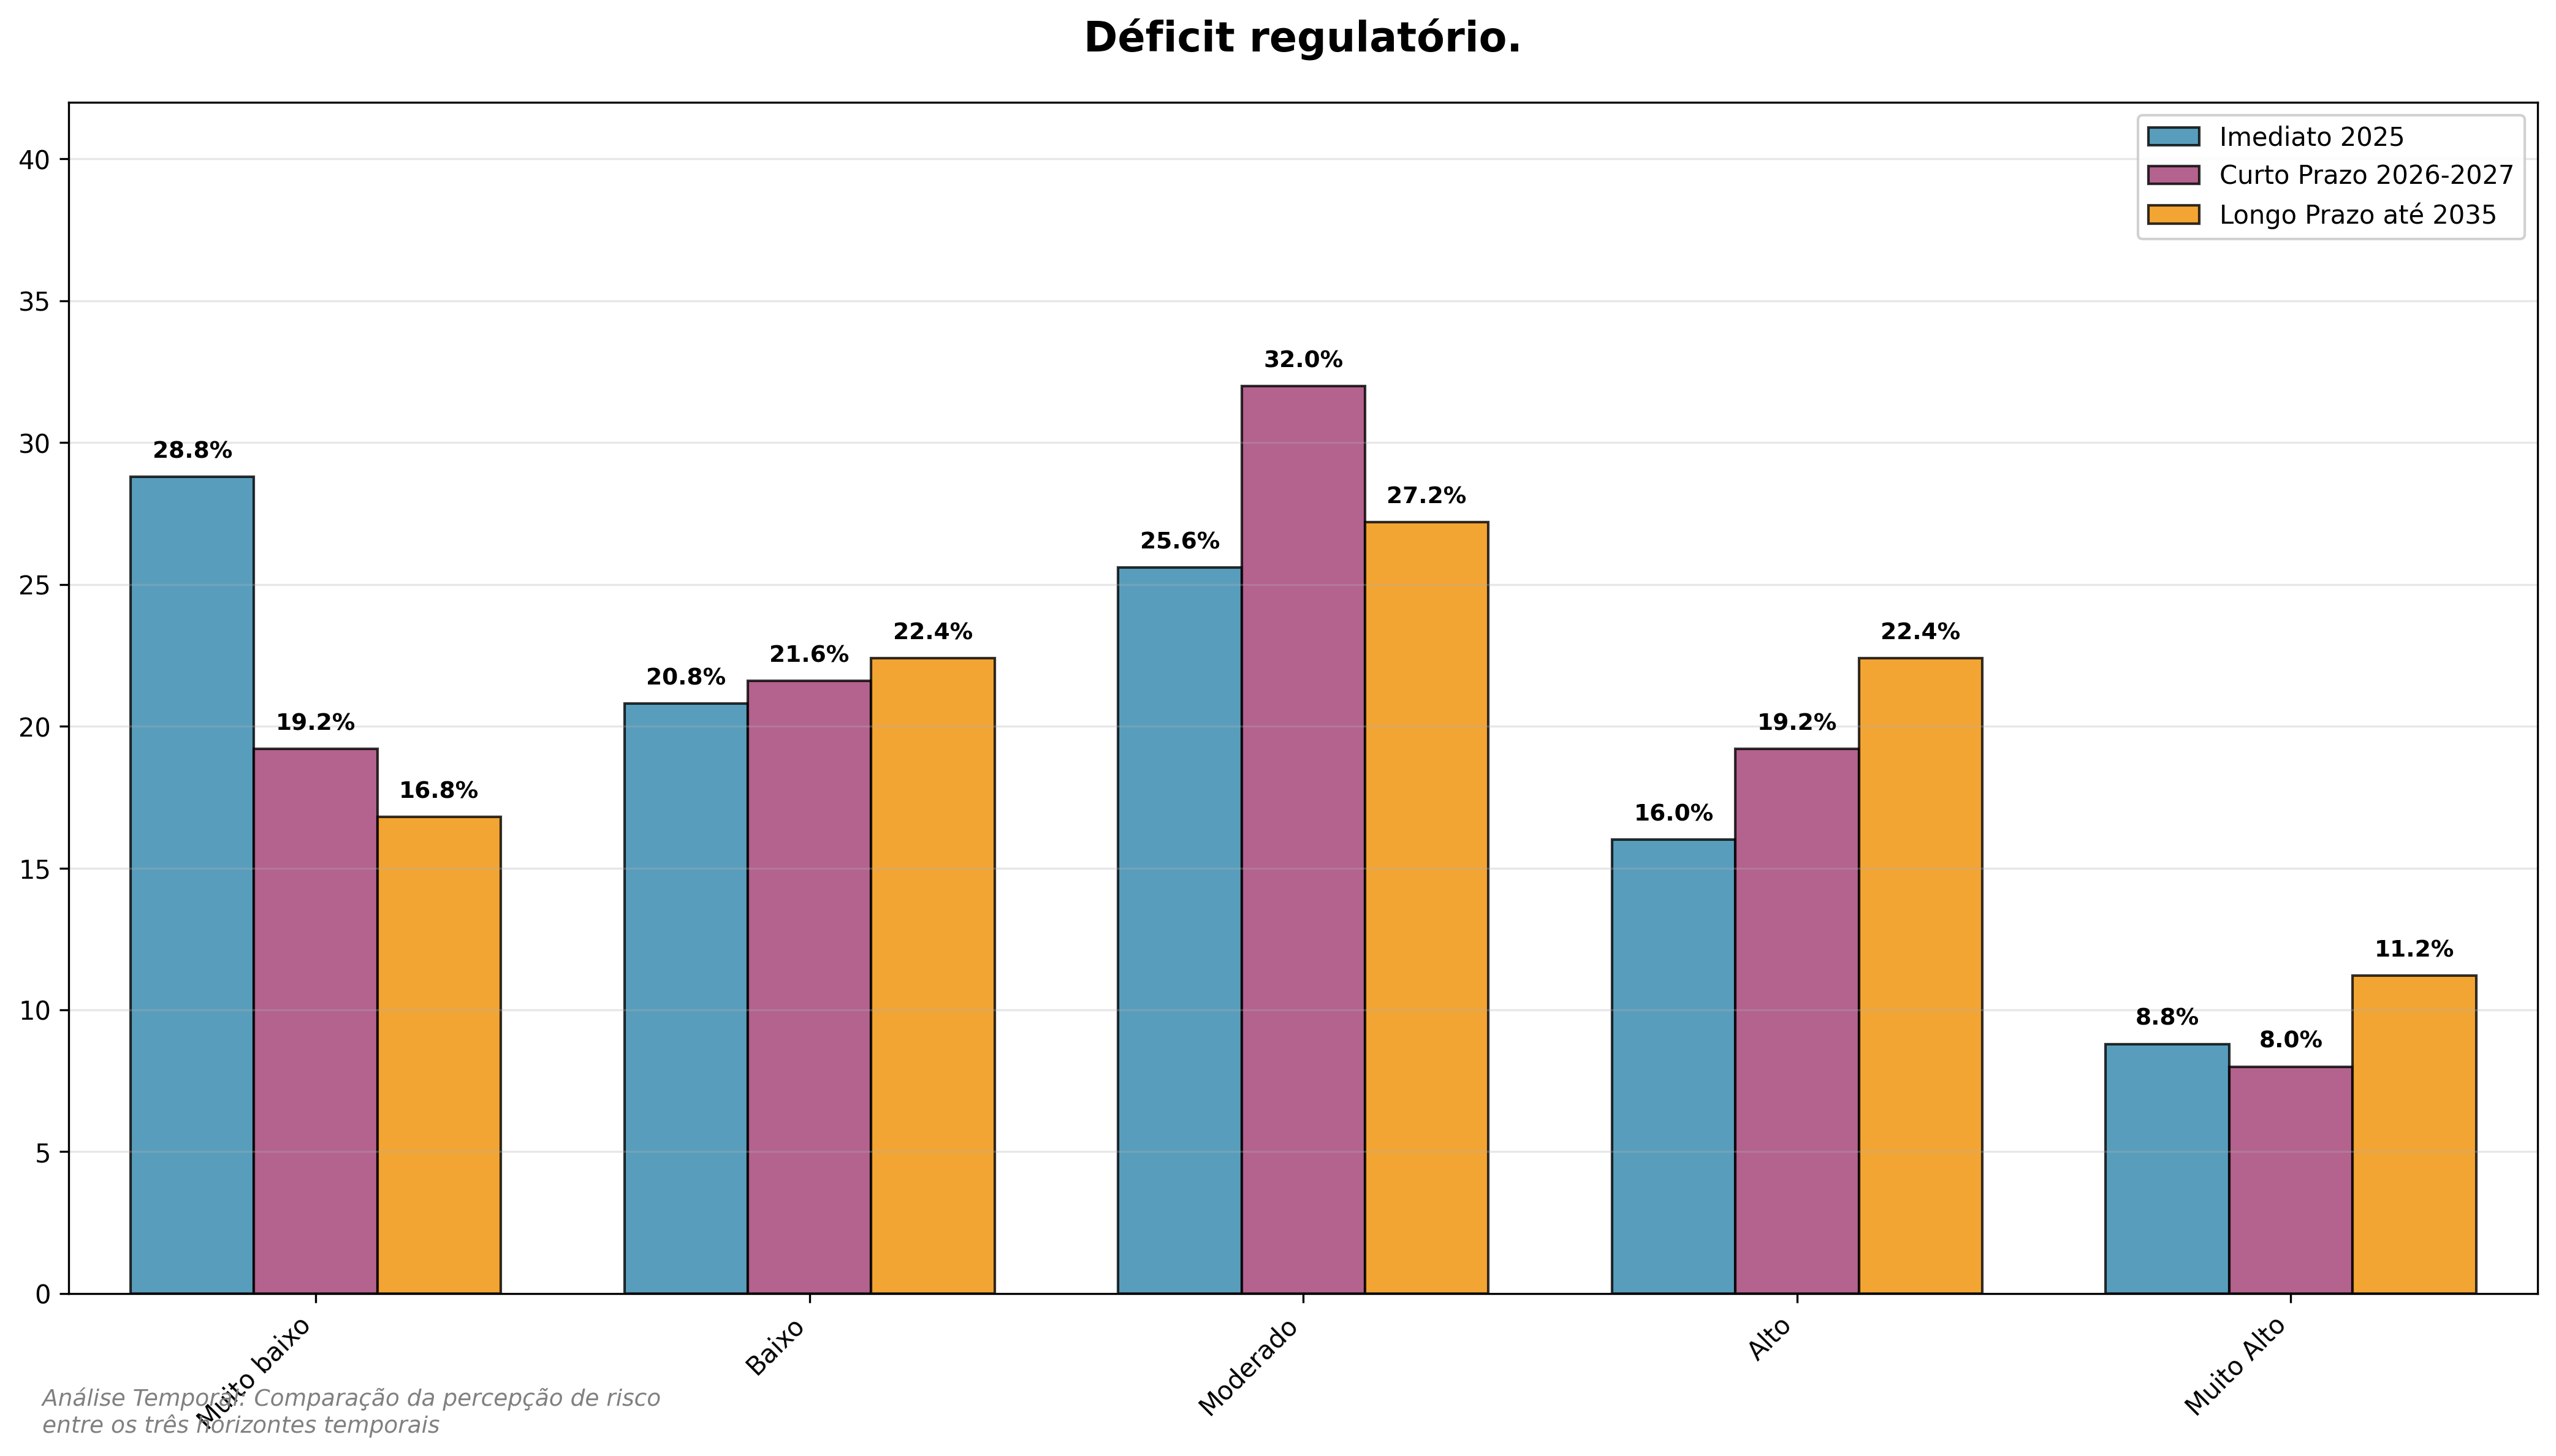
\includegraphics[keepaspectratio]{assets/economicos/grafico_agrupado_1_17_temporal.png}}

\begin{tcolorbox}[enhanced jigsaw, titlerule=0mm, colback=white, title=\textcolor{quarto-callout-tip-color}{\faLightbulb}\hspace{0.5em}{Destaques}, opacityback=0, colbacktitle=quarto-callout-tip-color!10!white, leftrule=.75mm, left=2mm, colframe=quarto-callout-tip-color-frame, bottomrule=.15mm, bottomtitle=1mm, breakable, toprule=.15mm, toptitle=1mm, opacitybacktitle=0.6, arc=.35mm, coltitle=black, rightrule=.15mm]

\textbf{Imediato (2025)}: Mediana 3.0, 46\% em risco alto

\textbf{Curto Prazo (2026-2027)}: Mediana 3.0, 47\% em risco alto

\textbf{Longo Prazo (até 2035)}: Mediana 3.0, 48\% em risco alto

\begin{itemize}
\tightlist
\item
  \textbf{Tendência}: Percepção de risco relativamente estável ao longo
  do tempo. \textbf{Déficit regulatório.}
\end{itemize}

Risco associado aos Riscos 1.6 e 1.7, ou seja, a evolução rápida de
condições de mercado e, principalmente, da tecnologia pode levar à
necessidade da adequação da regulamentação a novas situações e
condicionantes.

\end{tcolorbox}

\subsection{Desemprego}\label{desemprego}

O gr?fico a seguir apresenta a evolu??o temporal do risco Desemprego.
\pandocbounded{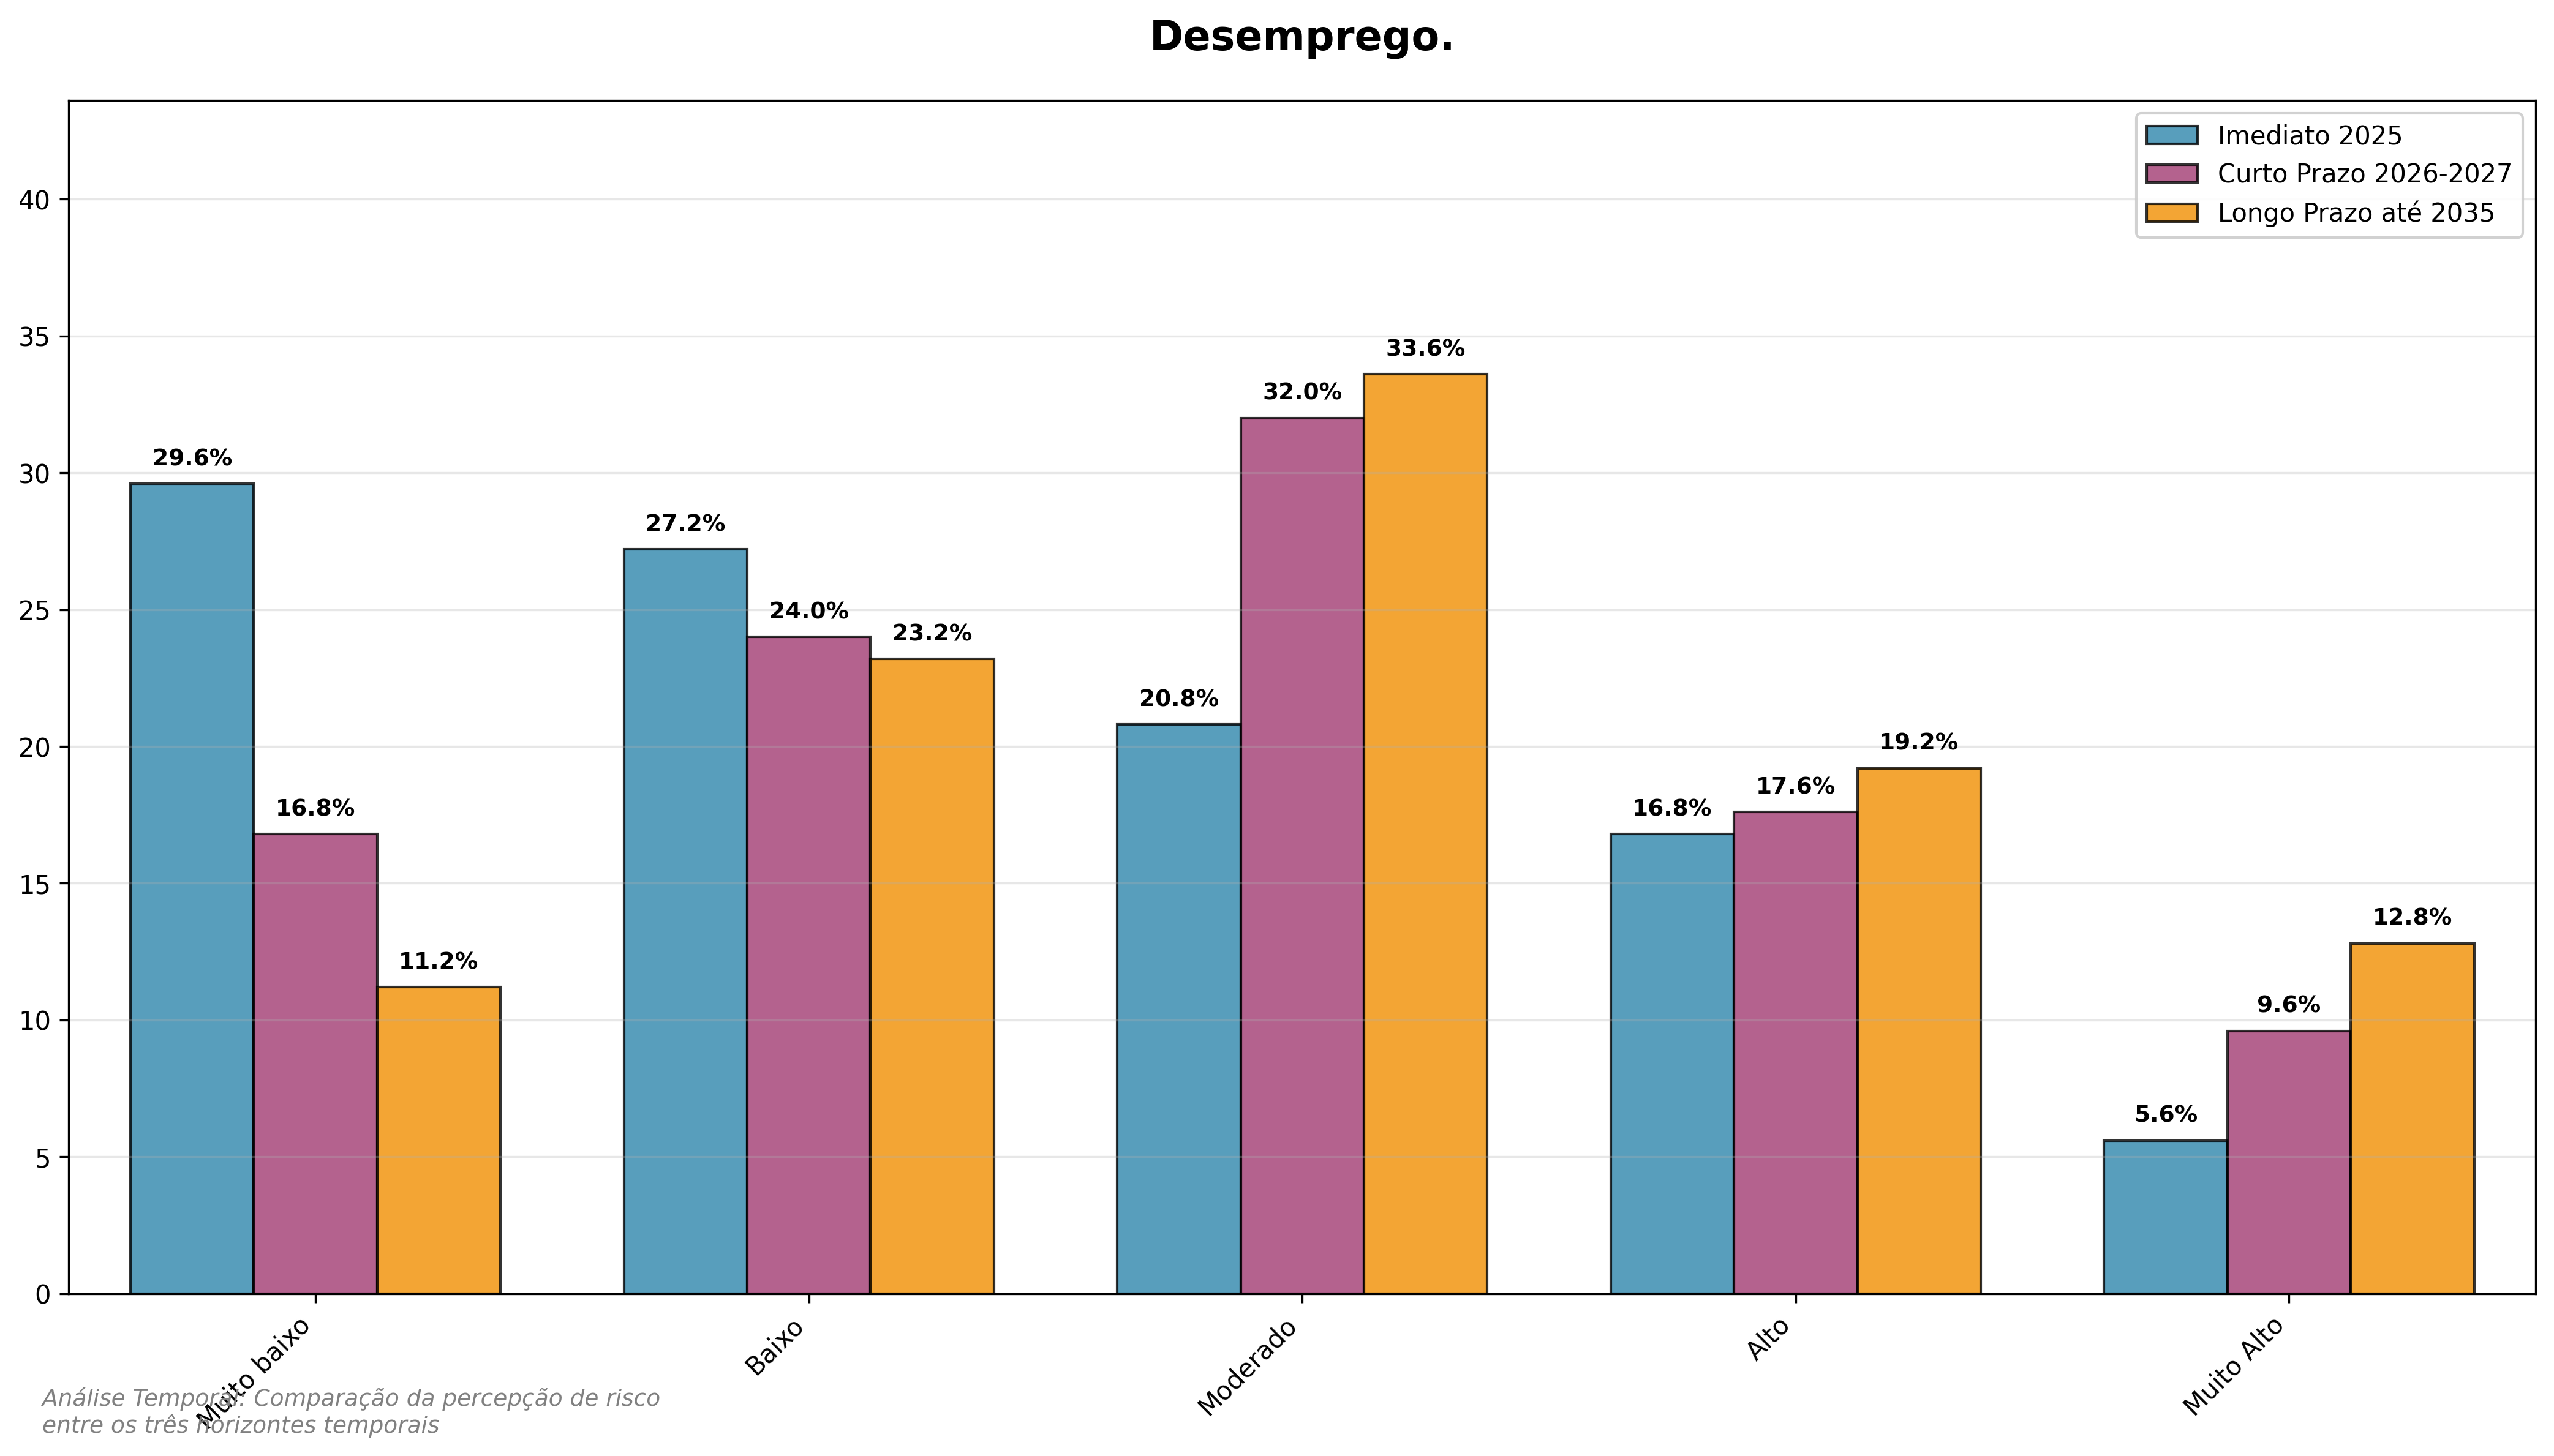
\includegraphics[keepaspectratio]{assets/economicos/grafico_agrupado_1_18_temporal.png}}

\begin{tcolorbox}[enhanced jigsaw, titlerule=0mm, colback=white, title=\textcolor{quarto-callout-tip-color}{\faLightbulb}\hspace{0.5em}{Destaques}, opacityback=0, colbacktitle=quarto-callout-tip-color!10!white, leftrule=.75mm, left=2mm, colframe=quarto-callout-tip-color-frame, bottomrule=.15mm, bottomtitle=1mm, breakable, toprule=.15mm, toptitle=1mm, opacitybacktitle=0.6, arc=.35mm, coltitle=black, rightrule=.15mm]

\textbf{Imediato (2025)}: Mediana 3.0, 30\% em risco alto

\textbf{Curto Prazo (2026-2027)}: Mediana 3.0, 36\% em risco alto

\textbf{Longo Prazo (até 2035)}: Mediana 3.0, 40\% em risco alto

\begin{itemize}
\tightlist
\item
  \textbf{Tendência}: Percepção de risco relativamente estável ao longo
  do tempo. \textbf{Desemprego}
\end{itemize}

Risco associado à evolução das atividades. Portos são serviços de
demanda derivada, ou seja, dependem do mercado dos produtos
movimentados. Outro fator importante é a evolução tecnológica e digital
com a eliminação de postos de trabalho, o que leva à necessidade de
desenvolvimento permanente do pessoal ocupado e controle das condições
de trabalho e contratação.

\end{tcolorbox}

\subsection{Corrupção}\label{corrupuxe7uxe3o}

O gr?fico a seguir apresenta a evolu??o temporal do risco Corrupção.
\pandocbounded{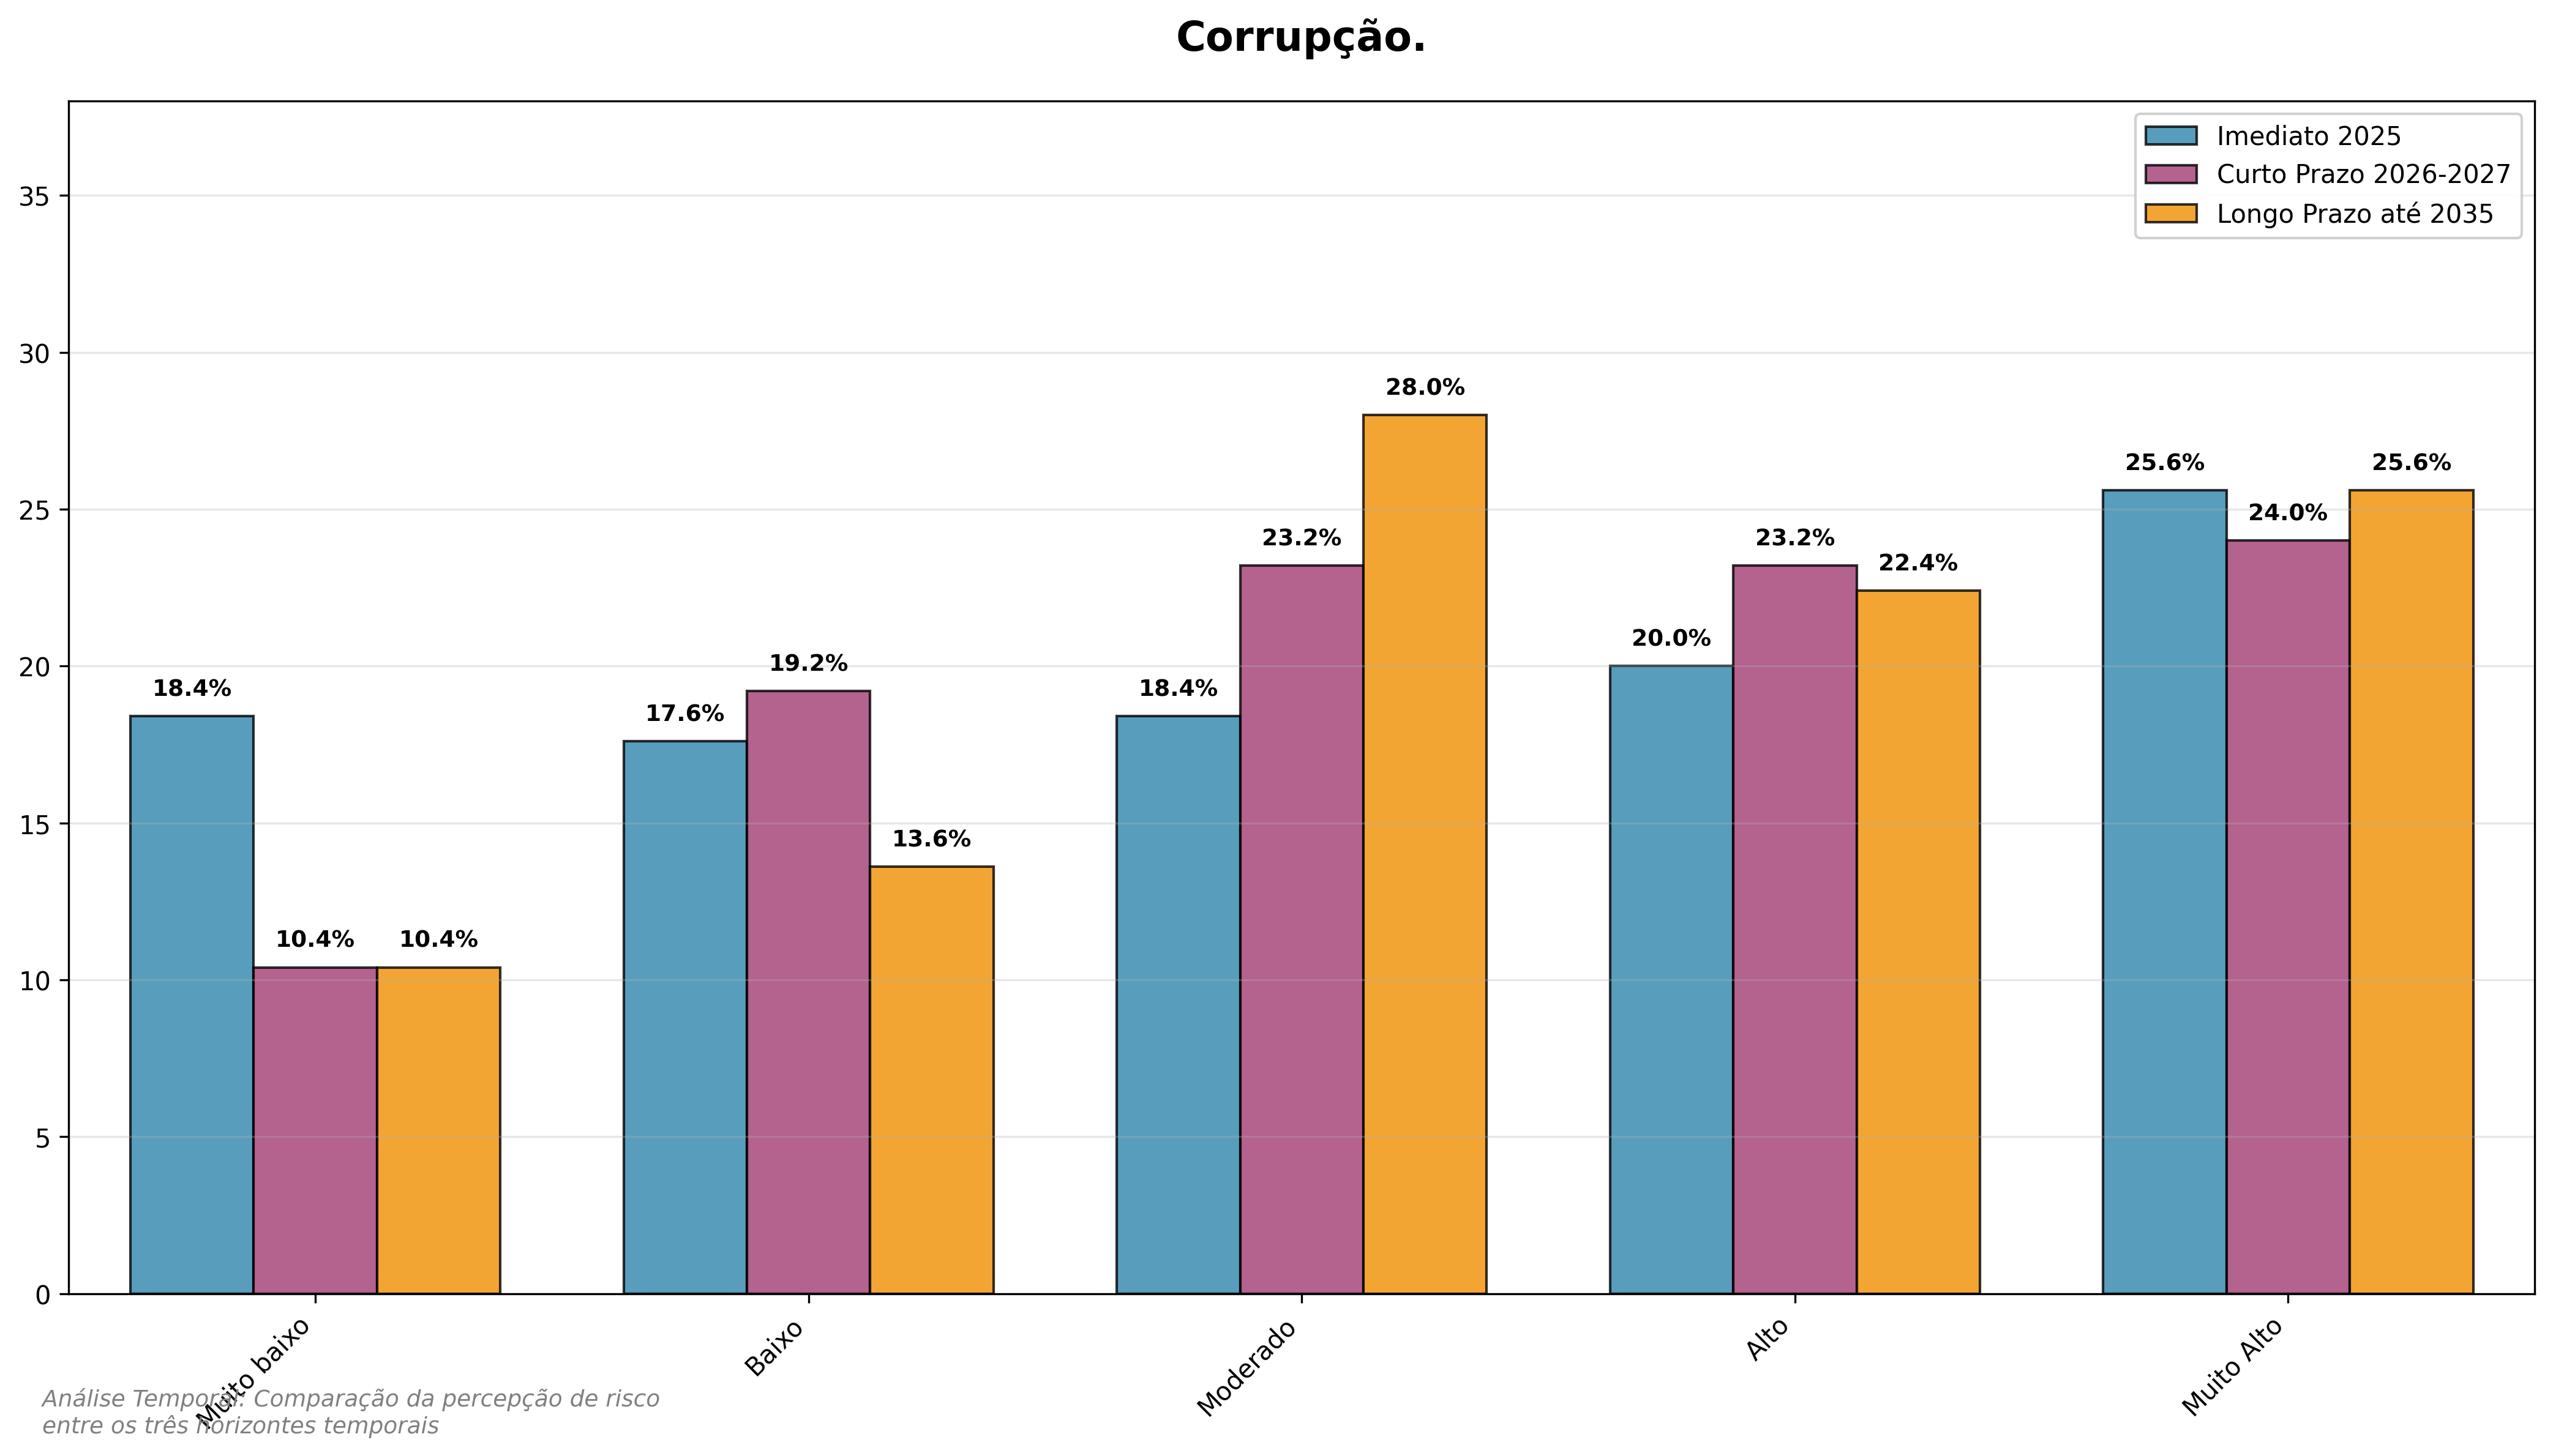
\includegraphics[keepaspectratio]{assets/economicos/grafico_agrupado_1_19_temporal.png}}

\begin{tcolorbox}[enhanced jigsaw, titlerule=0mm, colback=white, title=\textcolor{quarto-callout-tip-color}{\faLightbulb}\hspace{0.5em}{Destaques}, opacityback=0, colbacktitle=quarto-callout-tip-color!10!white, leftrule=.75mm, left=2mm, colframe=quarto-callout-tip-color-frame, bottomrule=.15mm, bottomtitle=1mm, breakable, toprule=.15mm, toptitle=1mm, opacitybacktitle=0.6, arc=.35mm, coltitle=black, rightrule=.15mm]

\textbf{Imediato (2025)}: Mediana 3.0, 38\% em risco alto

\textbf{Curto Prazo (2026-2027)}: Mediana 3.0, 46\% em risco alto

\textbf{Longo Prazo (até 2035)}: Mediana 3.0, 38\% em risco alto

\begin{itemize}
\tightlist
\item
  \textbf{Tendência}: Percepção de risco relativamente estável ao longo
  do tempo. \textbf{Corrupção.}
\end{itemize}

Risco associado ao Risco 1.9 e 1.12. As operações portuárias envolvem
muitos recursos e etapas variadas de realização, estando vulneráveis a
práticas inadequadas. Um controle rigoroso é necessário que se estende a
todas as cadeias produtivas envolvidas na atividade portuária.

\end{tcolorbox}

\subsection{Desequilíbrio econômico
regional}\label{desequiluxedbrio-econuxf4mico-regional}

O gr?fico a seguir apresenta a evolu??o temporal do risco Desequilíbrio
econômico regional.
\pandocbounded{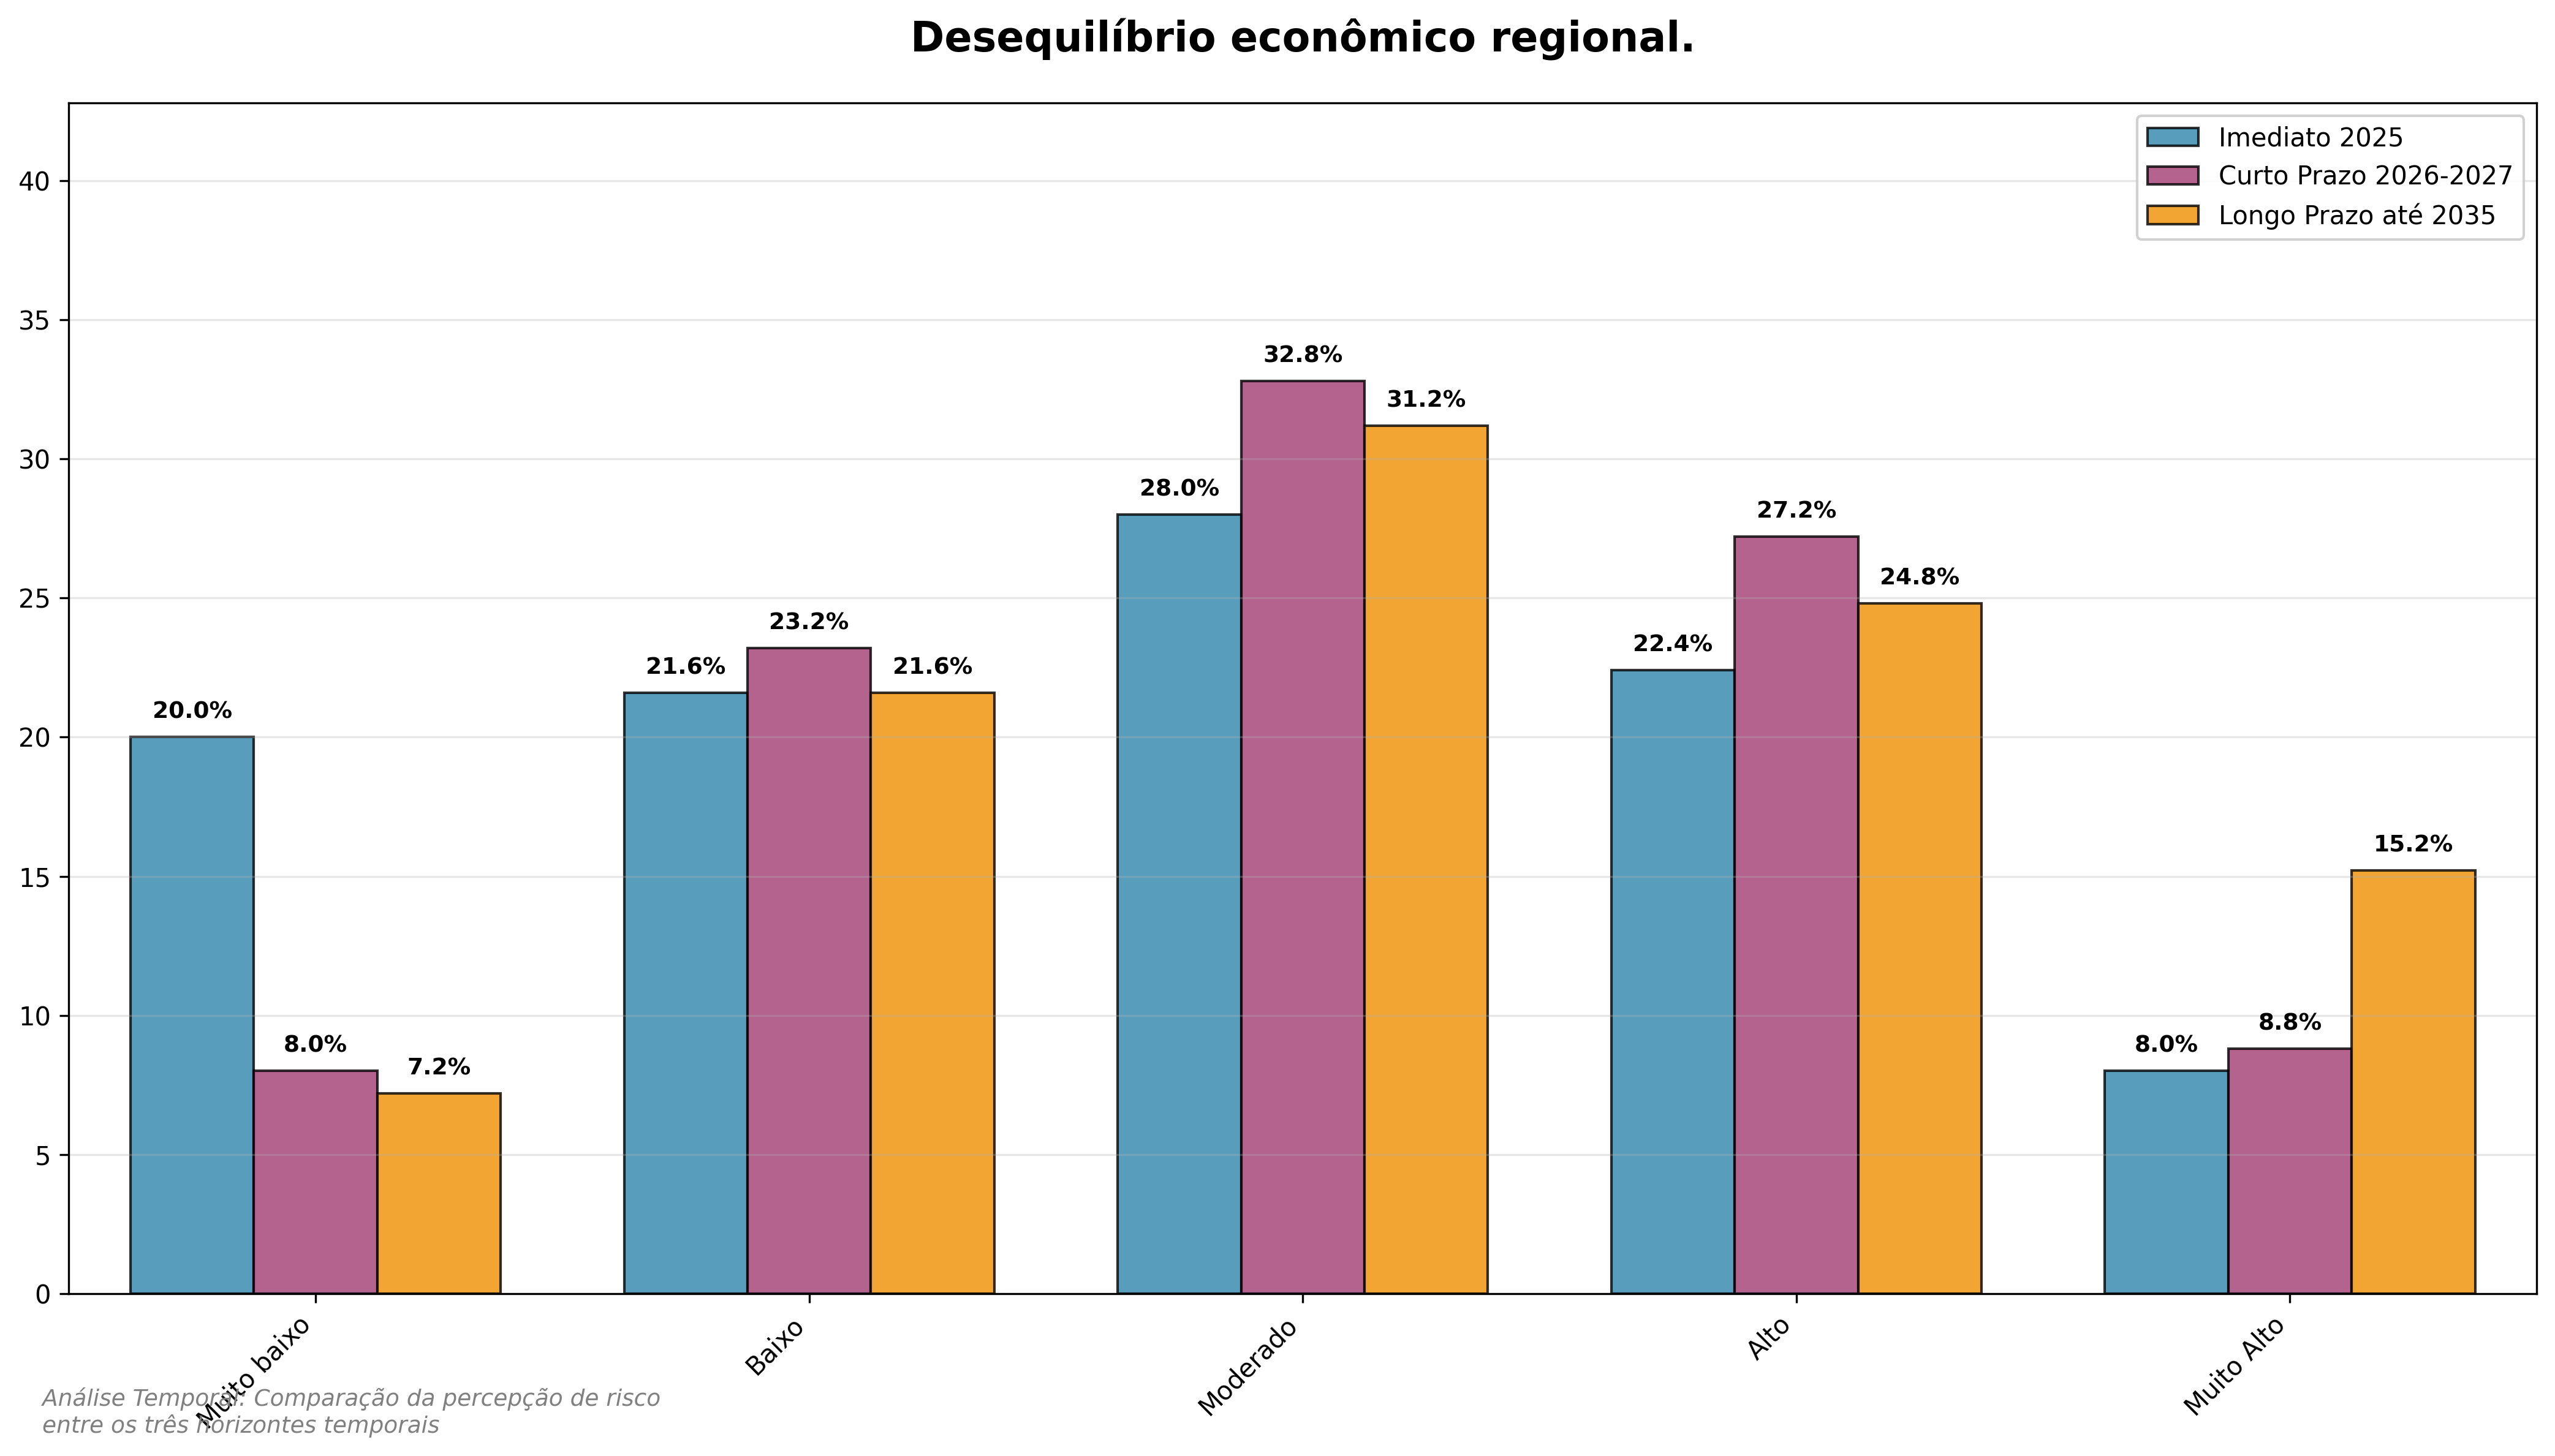
\includegraphics[keepaspectratio]{assets/economicos/grafico_agrupado_1_20_temporal.png}}

\begin{tcolorbox}[enhanced jigsaw, titlerule=0mm, colback=white, title=\textcolor{quarto-callout-tip-color}{\faLightbulb}\hspace{0.5em}{Destaques}, opacityback=0, colbacktitle=quarto-callout-tip-color!10!white, leftrule=.75mm, left=2mm, colframe=quarto-callout-tip-color-frame, bottomrule=.15mm, bottomtitle=1mm, breakable, toprule=.15mm, toptitle=1mm, opacitybacktitle=0.6, arc=.35mm, coltitle=black, rightrule=.15mm]

\textbf{Imediato (2025)}: Mediana 3.0, 30\% em risco alto

\textbf{Curto Prazo (2026-2027)}: Mediana 3.0, 36\% em risco alto

\textbf{Longo Prazo (até 2035)}: Mediana 3.0, 40\% em risco alto

\begin{itemize}
\tightlist
\item
  \textbf{Tendência}: Percepção de risco relativamente estável ao longo
  do tempo. \textbf{Desequilíbrio econômico regional.}
\end{itemize}

Risco decorrente da condição da operação portuária como de demanda
derivada. Portos têm sua atividade decorrente da economia de sua
hinterlândia, ou seja, sua área de atuação, ou as chamadas origens e
destinos verdadeiros dos produtos movimentados.

\end{tcolorbox}

\subsection{Conflito ou instabilidade institucional do
Estado}\label{conflito-ou-instabilidade-institucional-do-estado}

O gr?fico a seguir apresenta a evolu??o temporal do risco Conflito ou
instabilidade institucional do Estado.
\pandocbounded{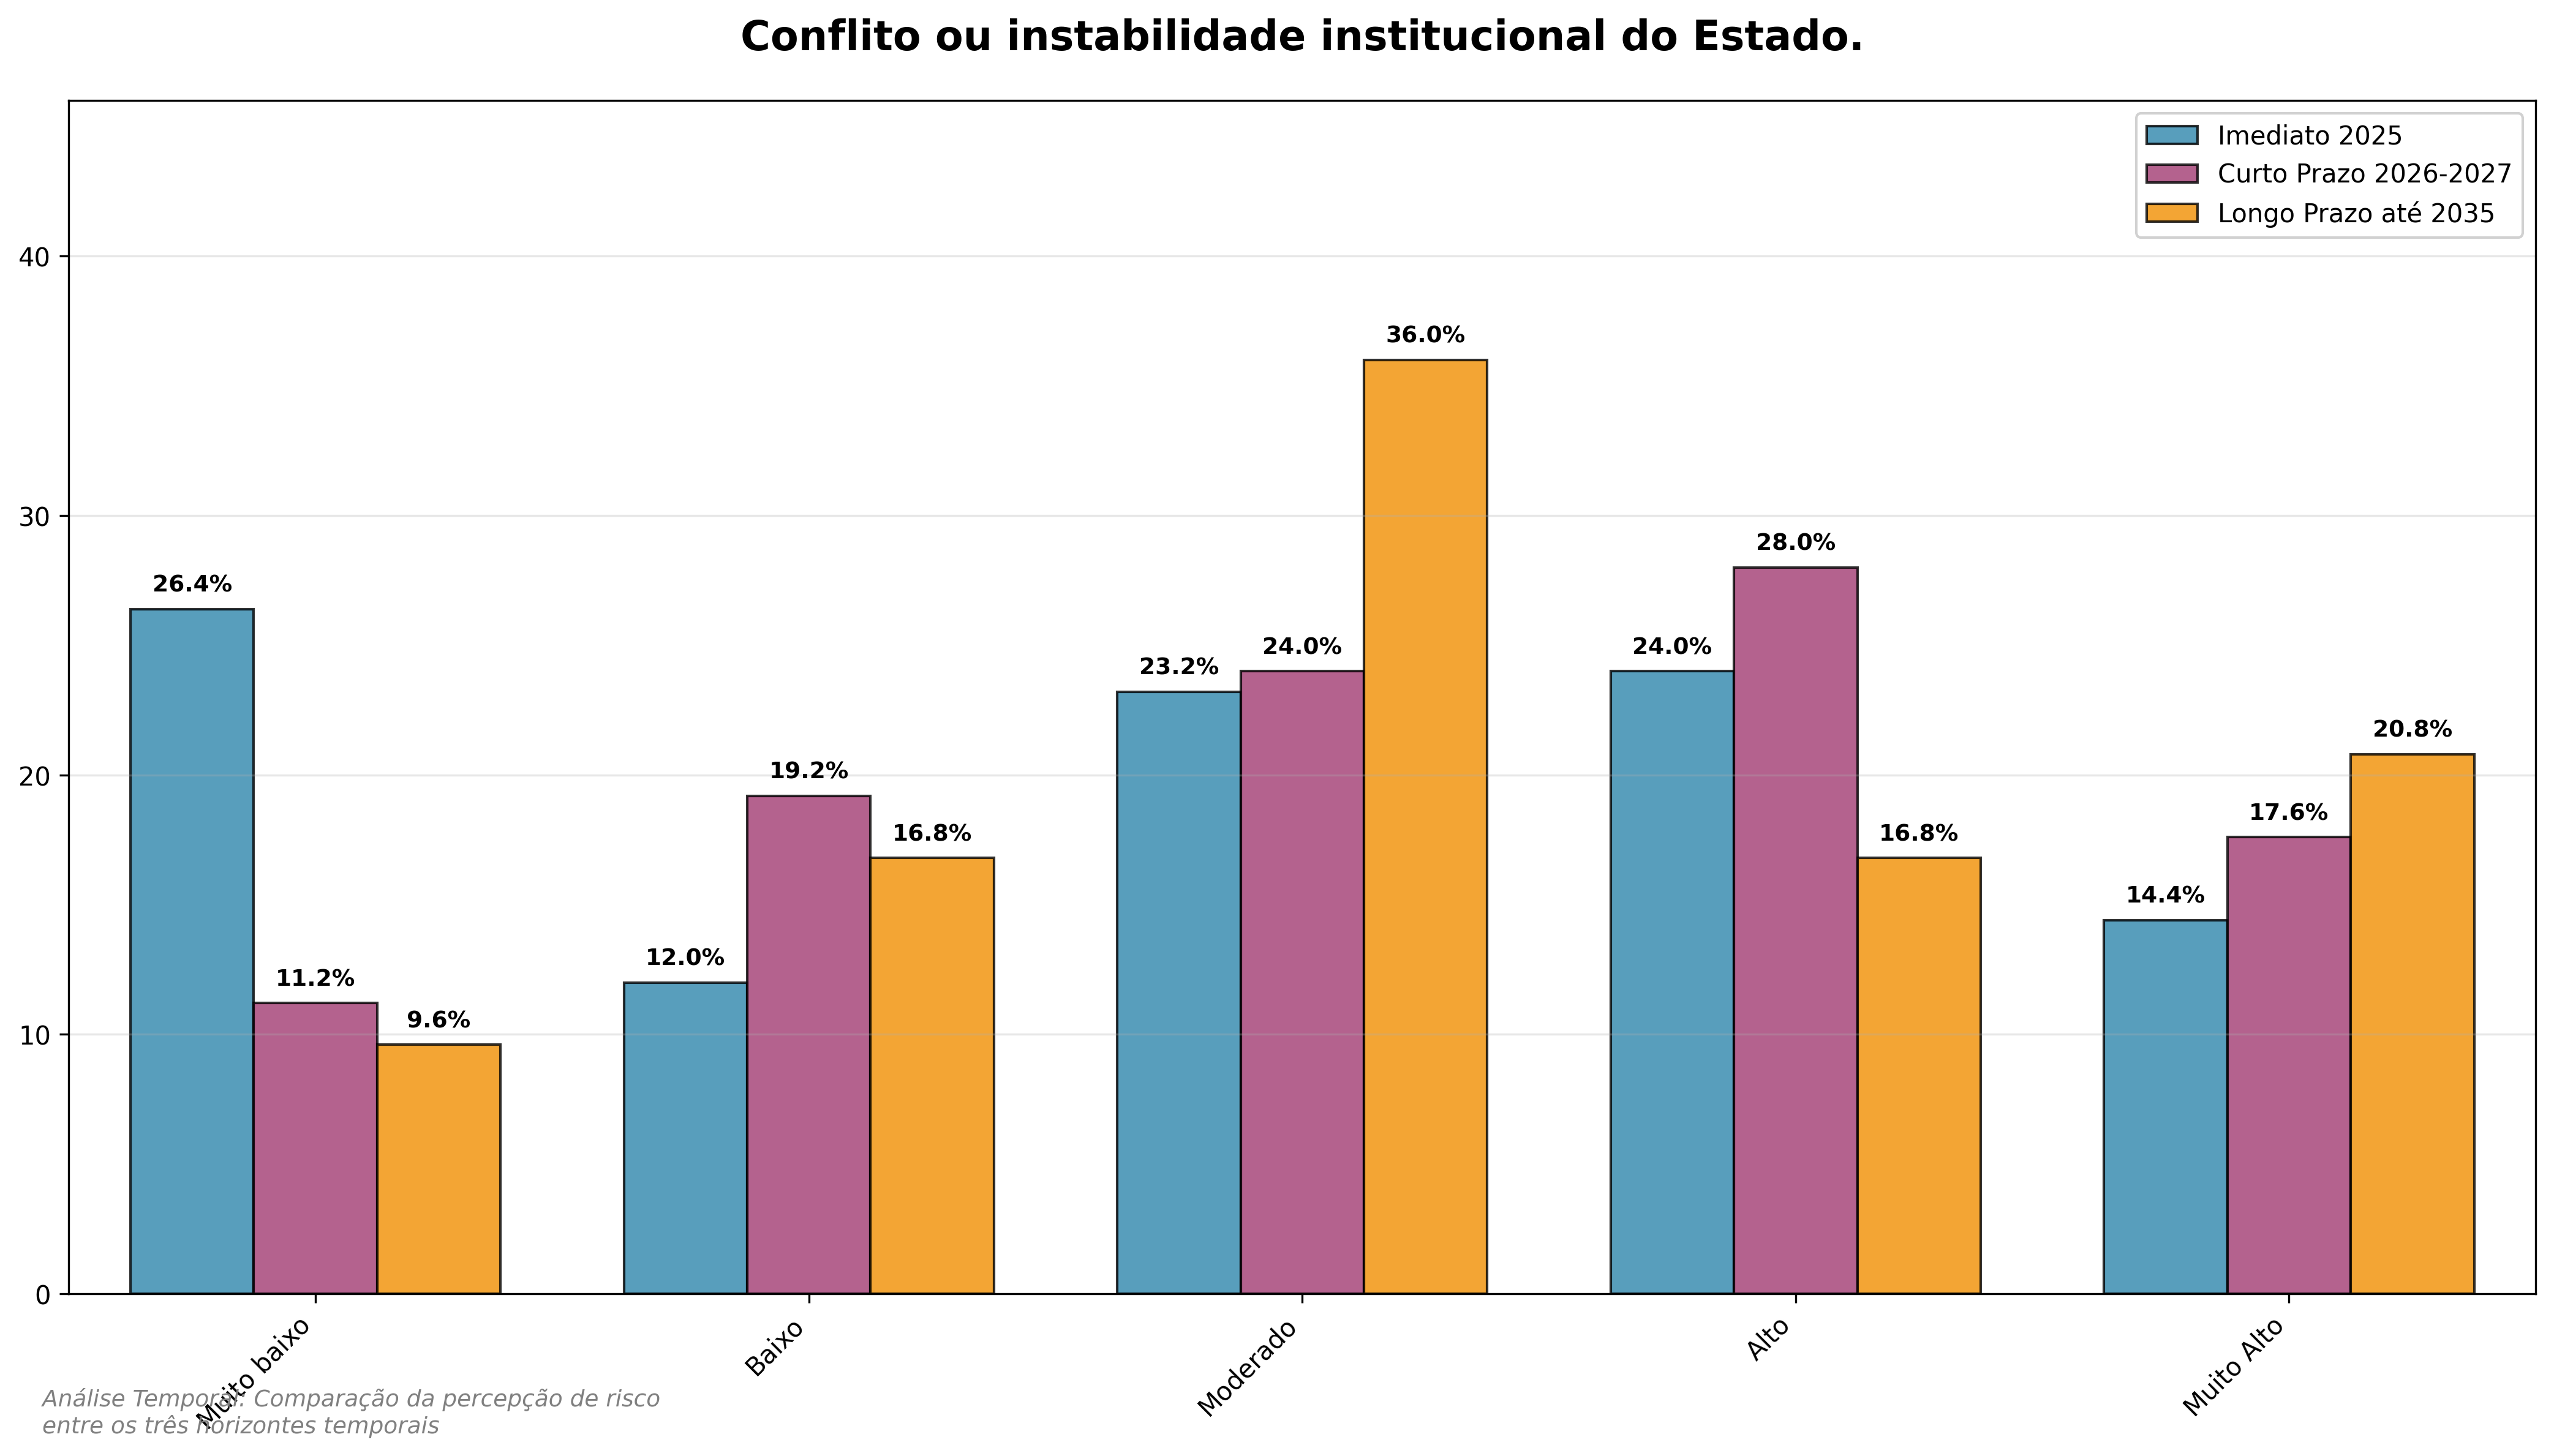
\includegraphics[keepaspectratio]{assets/economicos/grafico_agrupado_1_21_temporal.png}}

\begin{tcolorbox}[enhanced jigsaw, titlerule=0mm, colback=white, title=\textcolor{quarto-callout-tip-color}{\faLightbulb}\hspace{0.5em}{Destaques}, opacityback=0, colbacktitle=quarto-callout-tip-color!10!white, leftrule=.75mm, left=2mm, colframe=quarto-callout-tip-color-frame, bottomrule=.15mm, bottomtitle=1mm, breakable, toprule=.15mm, toptitle=1mm, opacitybacktitle=0.6, arc=.35mm, coltitle=black, rightrule=.15mm]

\textbf{Imediato (2025)}: Mediana 3.0, 38\% em risco alto

\textbf{Curto Prazo (2026-2027)}: Mediana 3.0, 46\% em risco alto

\textbf{Longo Prazo (até 2035)}: Mediana 3.0, 38\% em risco alto

\begin{itemize}
\tightlist
\item
  \textbf{Tendência}: Percepção de risco relativamente estável ao longo
  do tempo. \textbf{Conflito ou instabilidade institucional do Estado.
  {[}Imediato (2025){]}}
\end{itemize}

Riscos relativos à inserção das operações portuárias como elementos das
economias locais e regionais na dinâmica da relação com autoridades
públicas. Esse risco, naturalmente, abarca portos públicos e terminais
privados.

\end{tcolorbox}

\section{Análise Temporal
Comparativa}\label{anuxe1lise-temporal-comparativa}

A análise comparativa entre os horizontes temporais revela importantes
padrões:

\subsection{Tendências Identificadas}\label{tenduxeancias-identificadas}

\begin{itemize}
\tightlist
\item
  \textbf{Riscos Imediatos}: Maior preocupação com instabilidade
  econômica global e interrupção de cadeias de suprimentos;-
  \textbf{Riscos de Curto Prazo}: Destaque para aumento de custos
  operacionais e redução da demanda;- \textbf{Riscos de Longo Prazo}:
  Preocupação crescente com perda de competitividade e redução de
  investimentos. \#\#\# Insights Estratégicos
\end{itemize}

\begin{enumerate}
\def\labelenumi{\arabic{enumi}.}
\tightlist
\item
  \textbf{Resiliência Financeira}: Necessidade de fortalecer o capital
  de giro e diversificar fontes de receita;2. \textbf{Gestão de Custos}:
  Implementar programas de eficiência operacional e otimização
  logística;3. \textbf{Diversificação}: Reduzir dependência de mercados
  e clientes específicos;4. \textbf{Inovação}: Investir em tecnologias
  que aumentem a competitividade e reduzam custos. :::
  \{.content-visible when-format=``docx''\}
\end{enumerate}

:::

\bookmarksetup{startatroot}

\chapter{Riscos Ambientais}\label{riscos-ambientais-1}

Esta seção apresenta a análise detalhada dos riscos ambientais
identificados no questionário, organizados por horizontes temporais e
variáveis específicas.

\section{Visão Geral dos Riscos
Ambientais}\label{visuxe3o-geral-dos-riscos-ambientais}

Os riscos ambientais foram avaliados em três horizontes temporais:

\begin{itemize}
\tightlist
\item
  \textbf{Imediato (2025)}: Riscos que requerem atenção imediata;-
  \textbf{Curto Prazo (2026-2027)}: Riscos emergentes que demandam
  planejamento;- \textbf{Longo Prazo (até 2035)}: Riscos estratégicos
  que requerem visão de futuro. \#\# Panorama do Período Imediato
\end{itemize}

O gr?fico a seguir mostra a distribui??o dos riscos no per?odo imediato.
\pandocbounded{\includegraphics[keepaspectratio]{assets/ambientais/grafico_barras_imediato_2025.png}}

\begin{tcolorbox}[enhanced jigsaw, titlerule=0mm, colback=white, title=\textcolor{quarto-callout-note-color}{\faInfo}\hspace{0.5em}{Destaques do período Imediato de 2025}, opacityback=0, colbacktitle=quarto-callout-note-color!10!white, leftrule=.75mm, left=2mm, colframe=quarto-callout-note-color-frame, bottomrule=.15mm, bottomtitle=1mm, breakable, toprule=.15mm, toptitle=1mm, opacitybacktitle=0.6, arc=.35mm, coltitle=black, rightrule=.15mm]

\begin{itemize}
\tightlist
\item
  \textbf{Licenciamento ambiental}: 29\% em níveis altos;-
  \textbf{Presença de agentes patogênicos}: 27\% em níveis altos;-
  \textbf{Mudanças climáticas (eventos extremos)}: 26\% em níveis altos.
  Os resultados mostram que os principais focos de atenção estão ligados
  à gestão institucional, aos riscos sanitários e aos eventos climáticos
  extremos, evidenciando a necessidade de controles robustos e operações
  resilientes.
\end{itemize}

O licenciamento ambiental aparece como o risco mais expressivo, com 29\%
das respostas em níveis altos (4-5). A percepção de atrasos ou não
conformidades indica risco direto para suspensão de obras, imposição de
medidas compensatórias e incertezas regulatórias, comprometendo
planejamento e execução.

Na sequência, destaca-se a presença de agentes patogênicos e
deficiências de saneamento, com 27\% das respostas em níveis altos. O
dado evidencia preocupação com riscos à saúde ocupacional e à imagem
institucional, reforçando a necessidade de investimentos contínuos em
infraestrutura sanitária e monitoramento microbiológico.

O terceiro risco mais relevante é o de mudanças climáticas, com 26\% das
respostas em níveis altos (4--5). Eventos severos --- tempestades, marés
de tempestade ou ondas de calor --- podem afetar diretamente a
infraestrutura portuária, a segurança operacional e a continuidade
logística.

\end{tcolorbox}

\section{Análise Temporal da Dimensão
Ambiental}\label{anuxe1lise-temporal-da-dimensuxe3o-ambiental}

O gr?fico a seguir sintetiza a evolu??o temporal das vari?veis da
dimens?o ambiental.
\pandocbounded{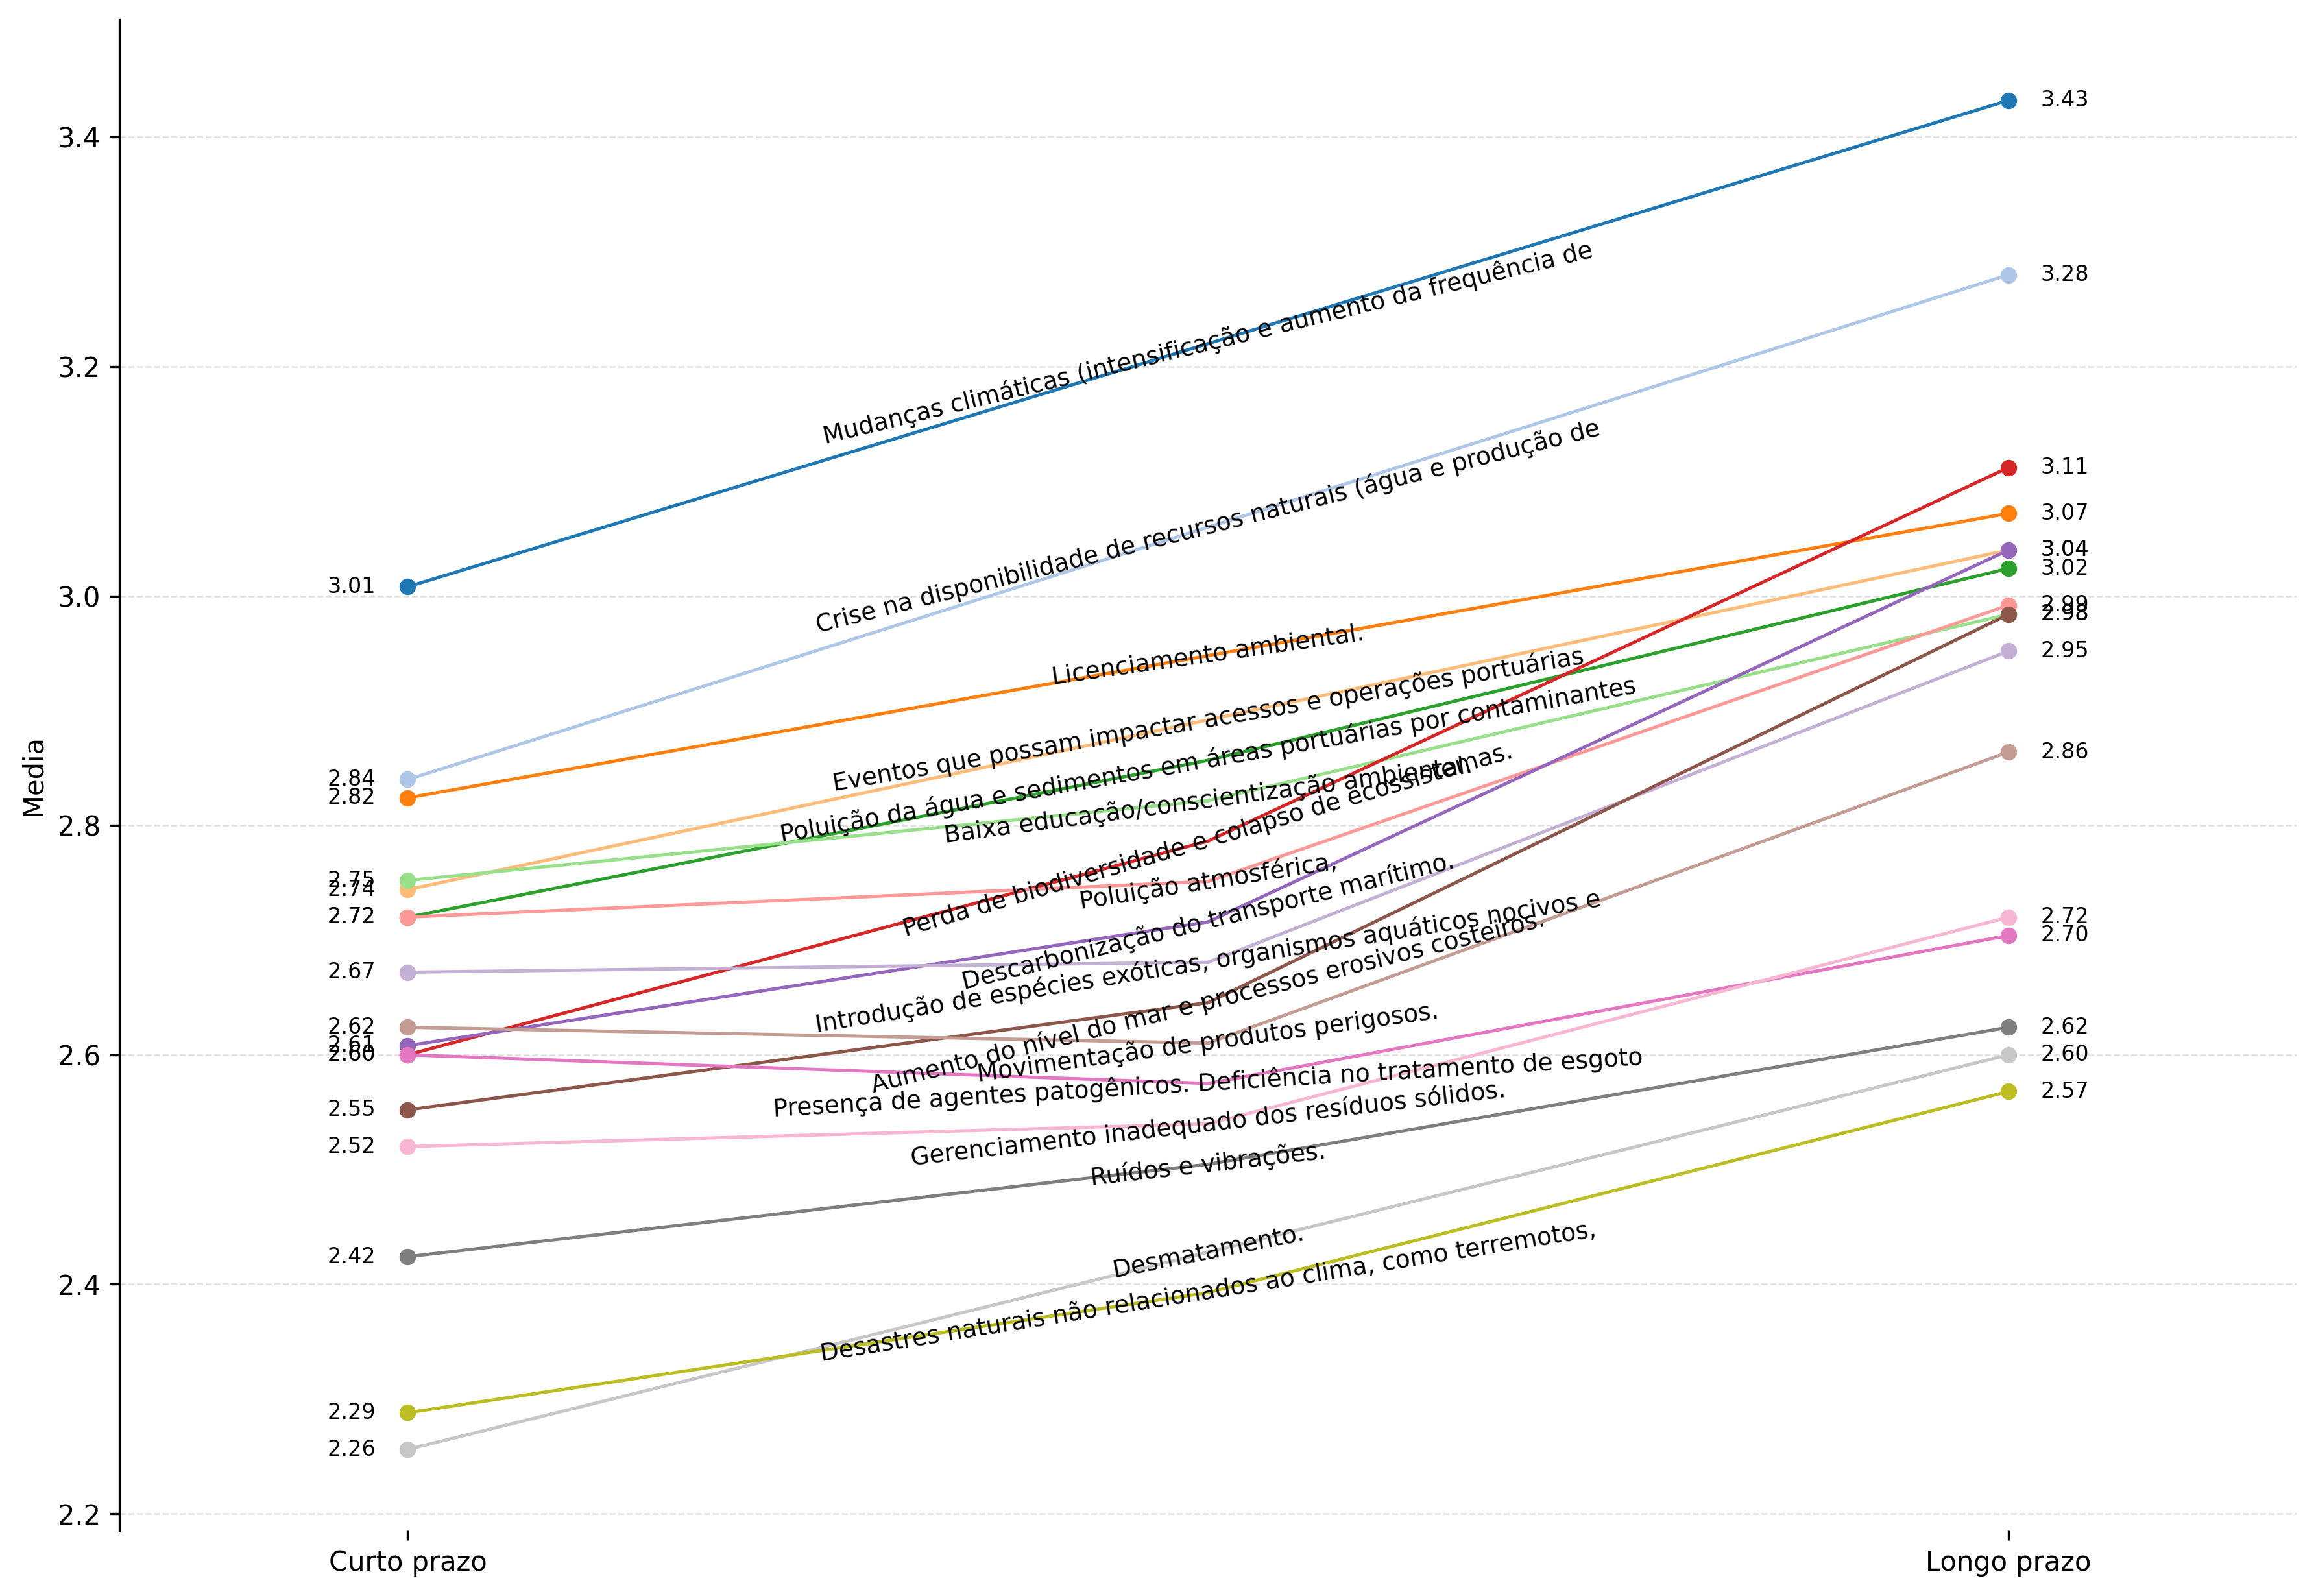
\includegraphics[keepaspectratio]{assets/slopegraphs_por_dimensao/slopegraph_ambiental.png}}

Os riscos ambientais refletem a crescente conscientização sobre questões
sustentáveis no setor portuário. A análise temporal mostra como as
percepções sobre impactos ambientais evoluem, indicando possíveis
mudanças nas prioridades de mitigação ao longo do tempo.

\subsection{Insights da Análise Temporal
Ambiental}\label{insights-da-anuxe1lise-temporal-ambiental}

A análise temporal dos riscos ambientais revela o padrão mais
preocupante entre todas as dimensões:

\subsubsection{Piora Ambiental
Significativa}\label{piora-ambiental-significativa}

\begin{itemize}
\item
  \textbf{Delta médio de +0,56}: Maior piora entre todas as dimensões;-
  \textbf{9 variáveis com piora crítica (+1.0 ponto)}: Mudanças
  climáticas, aumento do nível do mar, poluição, espécies exóticas,
  resíduos, desmatamento, ruídos, patógenos, produtos perigosos;-
  \textbf{Tendência de deterioração acelerada}: A maioria dos riscos
  ambientais mostra piora progressiva. \#\#\#\# Padrões Específicos
  Identificados
\item
  \textbf{Mudanças Climáticas como Principal Risco}: Evolui de mediana
  2.0 para 4.0, tornando-se crítica;- \textbf{Riscos Costeiros em
  Ascensão}: Aumento do nível do mar e erosão costeira mostram piora
  significativa;- \textbf{Pressão Regulatória Crescente}: Licenciamento
  ambiental e descarbonização tornam-se mais críticos. \#\#\#\#
  Destaques da Evolução Temporal
\item
  \textbf{Risco Mais Crítico em 2035}: Aumento da temperatura média
  (52\% em risco alto);- \textbf{Maior Crescimento Relativo}:
  Desmatamento (+119\% no risco alto);- \textbf{Transformação
  Regulatória}: Descarbonização do transporte marítimo (+161\% no risco
  alto). \#\#\#\# Implicações Estratégicas para a Dimensão Ambiental
\end{itemize}

A análise temporal ambiental exige ação imediata:

1. \textbf{Adaptação Climática Urgente}: Investir em infraestrutura
resiliente a eventos extremos

2. \textbf{Transição para Baixo Carbono}: Acelerar planos de
descarbonização e energias renováveis

3. \textbf{Gestão Costeira Integrada}: Desenvolver estratégias para
proteção contra aumento do nível do mar

4. \textbf{Biodiversidade e Ecossistemas}: Implementar programas
robustos de conservação e restauração

\section{Exame das Variáveis de Risco: Resultados e
Tendências}\label{exame-das-variuxe1veis-de-risco-resultados-e-tenduxeancias-1}

\subsection{Perda de biodiversidade e colapso de
ecossistemas}\label{perda-de-biodiversidade-e-colapso-de-ecossistemas}

O gr?fico a seguir apresenta a evolu??o temporal do risco Perda de
biodiversidade e colapso de ecossistemas.
\pandocbounded{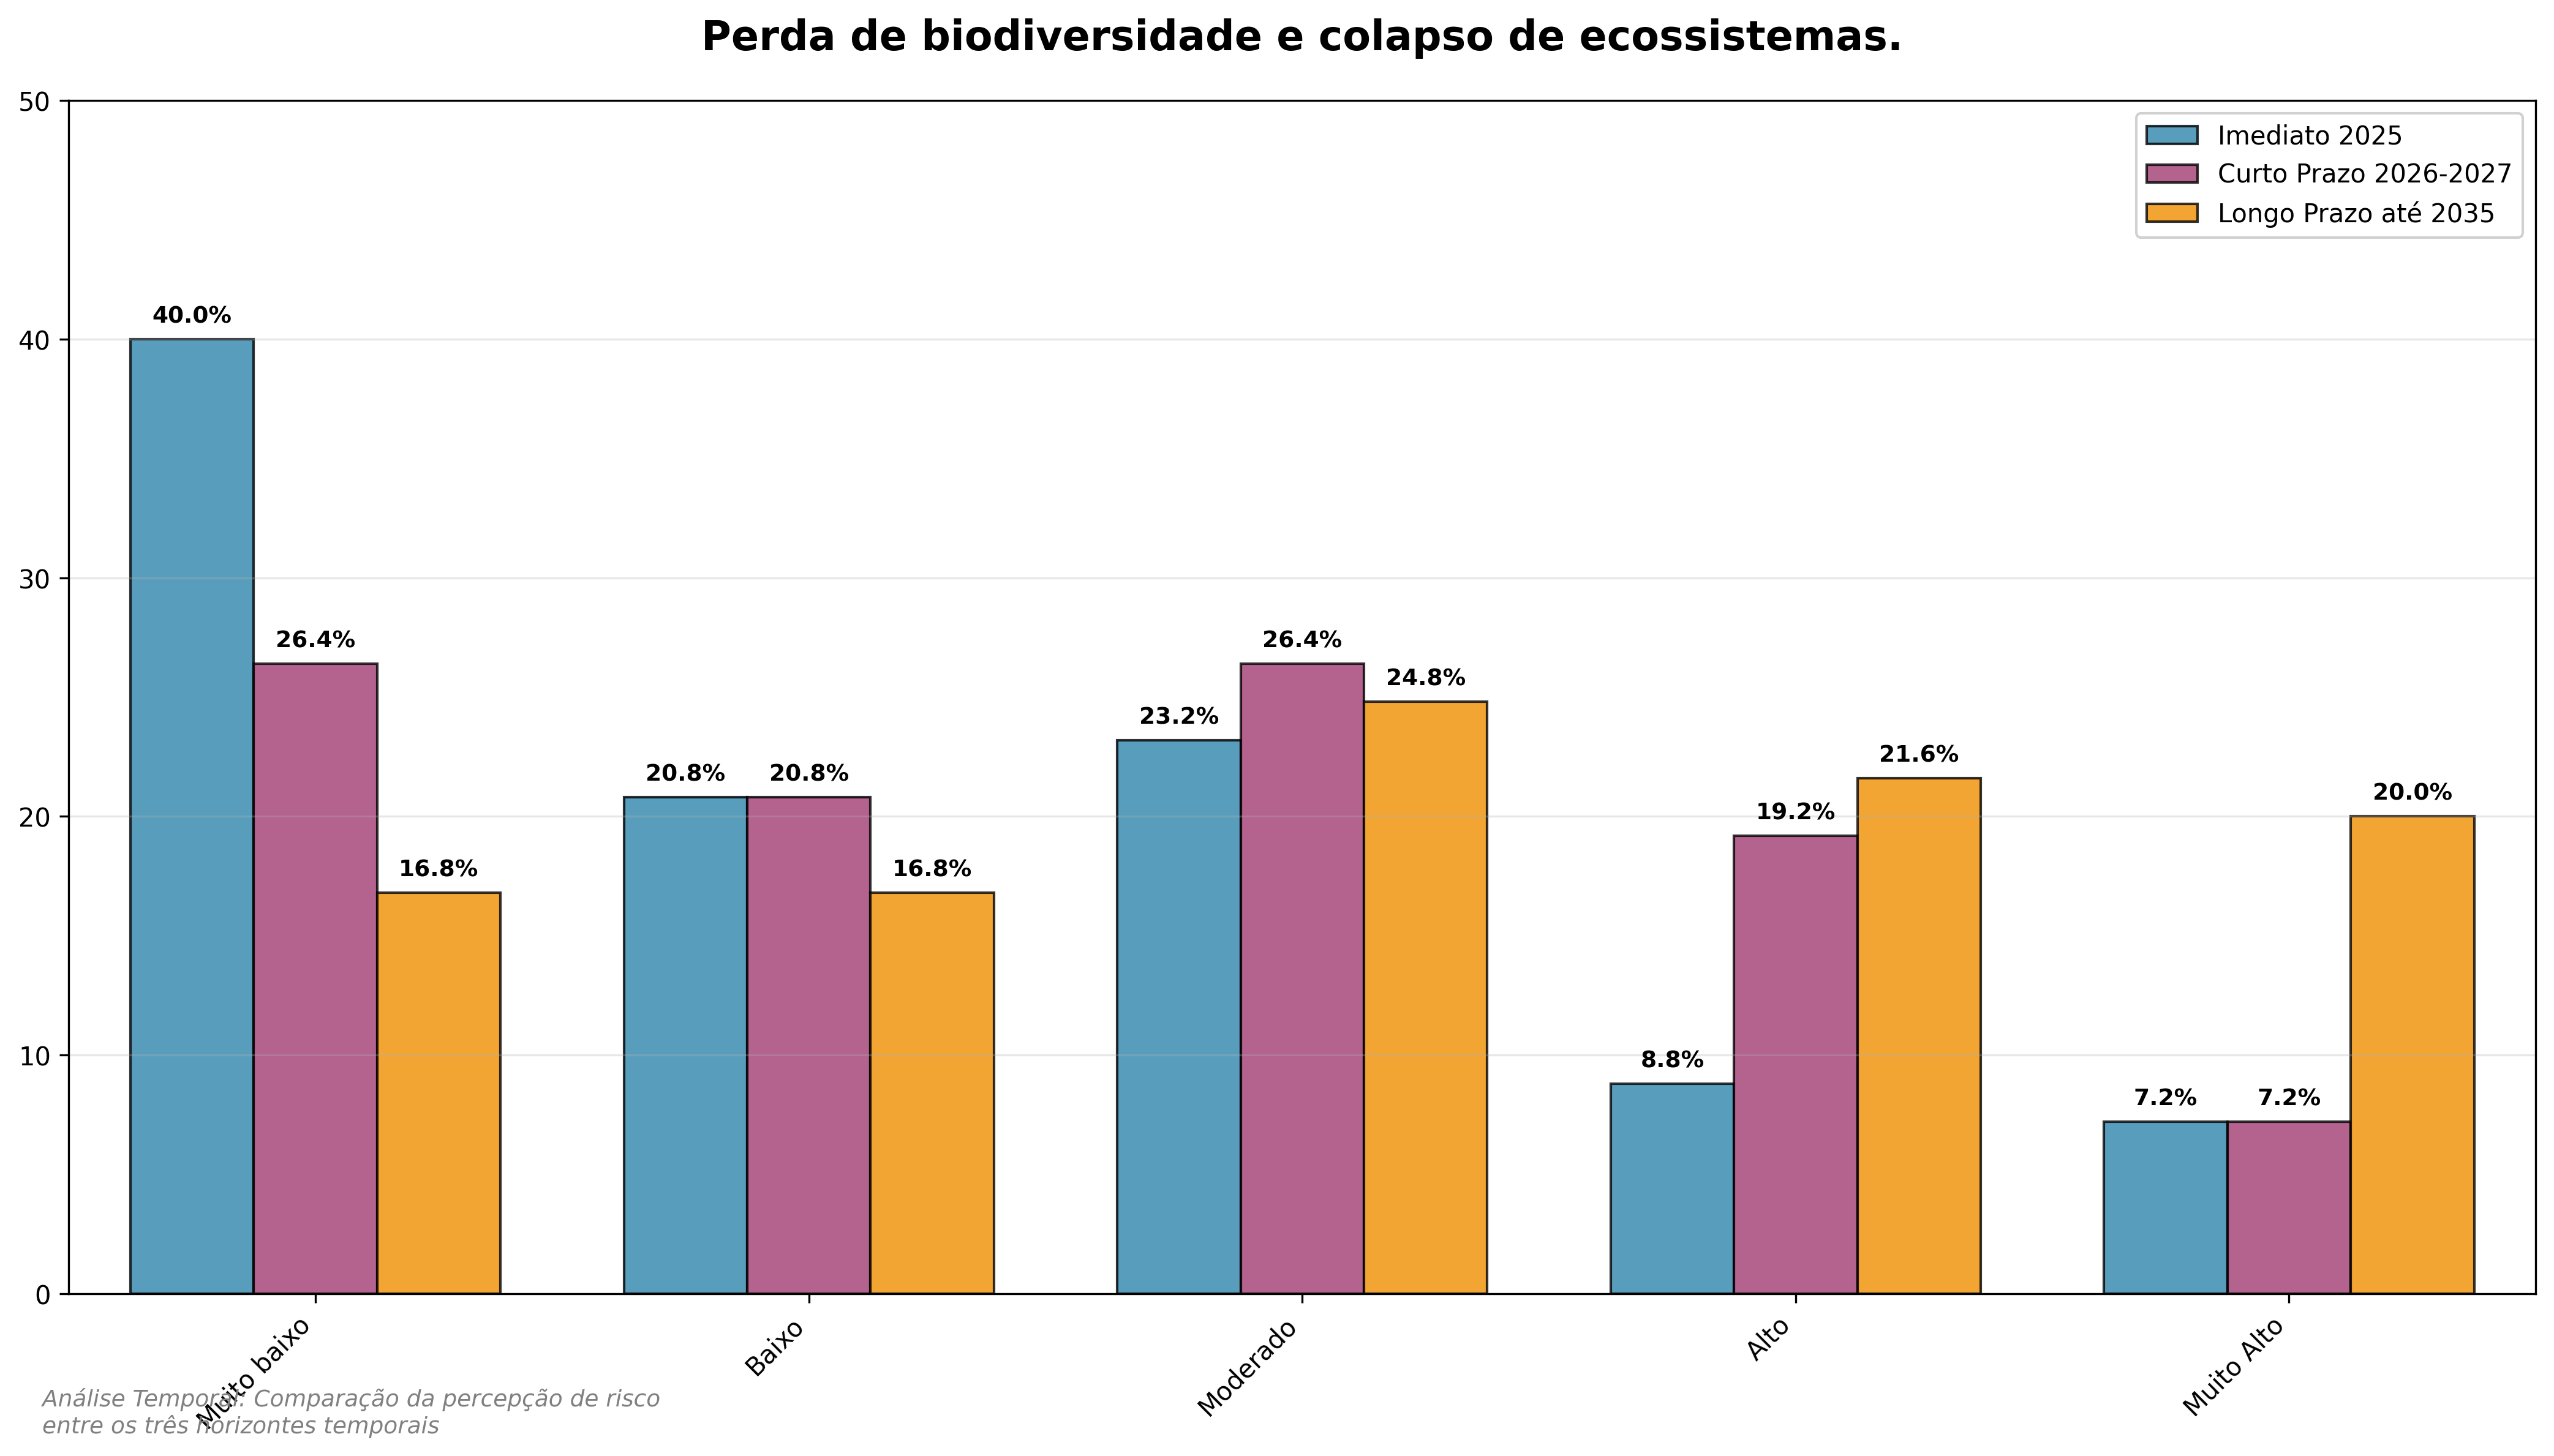
\includegraphics[keepaspectratio]{assets/ambientais/grafico_agrupado_2_1_temporal.png}}

\begin{tcolorbox}[enhanced jigsaw, titlerule=0mm, colback=white, title=\textcolor{quarto-callout-tip-color}{\faLightbulb}\hspace{0.5em}{Destaques}, opacityback=0, colbacktitle=quarto-callout-tip-color!10!white, leftrule=.75mm, left=2mm, colframe=quarto-callout-tip-color-frame, bottomrule=.15mm, bottomtitle=1mm, breakable, toprule=.15mm, toptitle=1mm, opacitybacktitle=0.6, arc=.35mm, coltitle=black, rightrule=.15mm]

\begin{longtable}[]{@{}
  >{\raggedright\arraybackslash}p{(\linewidth - 0\tabcolsep) * \real{1.0021}}@{}}
\toprule\noalign{}
\endhead
\bottomrule\noalign{}
\endlastfoot
\textbf{Evolução da Percepção de Risco}: Os dados mostram uma tendência
de aumento gradual na percepção de risco associada à perda de
biodiversidade e ao colapso dos ecossistemas ao longo do tempo.
Observa-se que à medida que o horizonte temporal se amplia cresce o
número de respondentes que classificam o risco como alto ou muito alto.

\textbf{Contexto Detalhado por Período:}

\textbf{Período Imediato (2025):} Apenas 16\% dos participantes percebem
o risco em níveis altos (4) ou muito altos (5), com mediana igual a 2.

\textbf{Curto Prazo (2026--2027):} A preocupação aumenta, com 26\% dos
respondentes avaliando o risco como alto ou muito alto, e mediana de 3,
sinalizando maior sensibilidade às possíveis ameaças ambientais.
\textbar{}

\textbf{Longo Prazo (até 2035):} A percepção de risco se intensifica
expressivamente, alcançando 42\% das respostas nos níveis 4-5, com
mediana também em 3, refletindo uma visão mais crítica e realista sobre
os impactos cumulativos da degradação ambiental. \textbar{}

\textbf{Implicações Estratégicas:} A perda de biodiversidade e o colapso
dos ecossistemas podem comprometer serviços ecossistêmicos essenciais,
como a proteção costeira, a manutenção da qualidade da água e o
equilíbrio das cadeias tróficas. Esses efeitos podem gerar restrições
operacionais, exigência de medidas compensatórias e conflitos
socioambientais, ameaçando a sustentabilidade ambiental do complexo
portuário e, consequentemente, a manutenção de suas licenças de
operação. \\
\end{longtable}

\end{tcolorbox}

\subsection{Eventos que possam impactar acessos e operações
portuárias}\label{eventos-que-possam-impactar-acessos-e-operauxe7uxf5es-portuuxe1rias}

O gr?fico a seguir apresenta a evolu??o temporal do risco Eventos que
possam impactar acessos e operações portuárias.
\pandocbounded{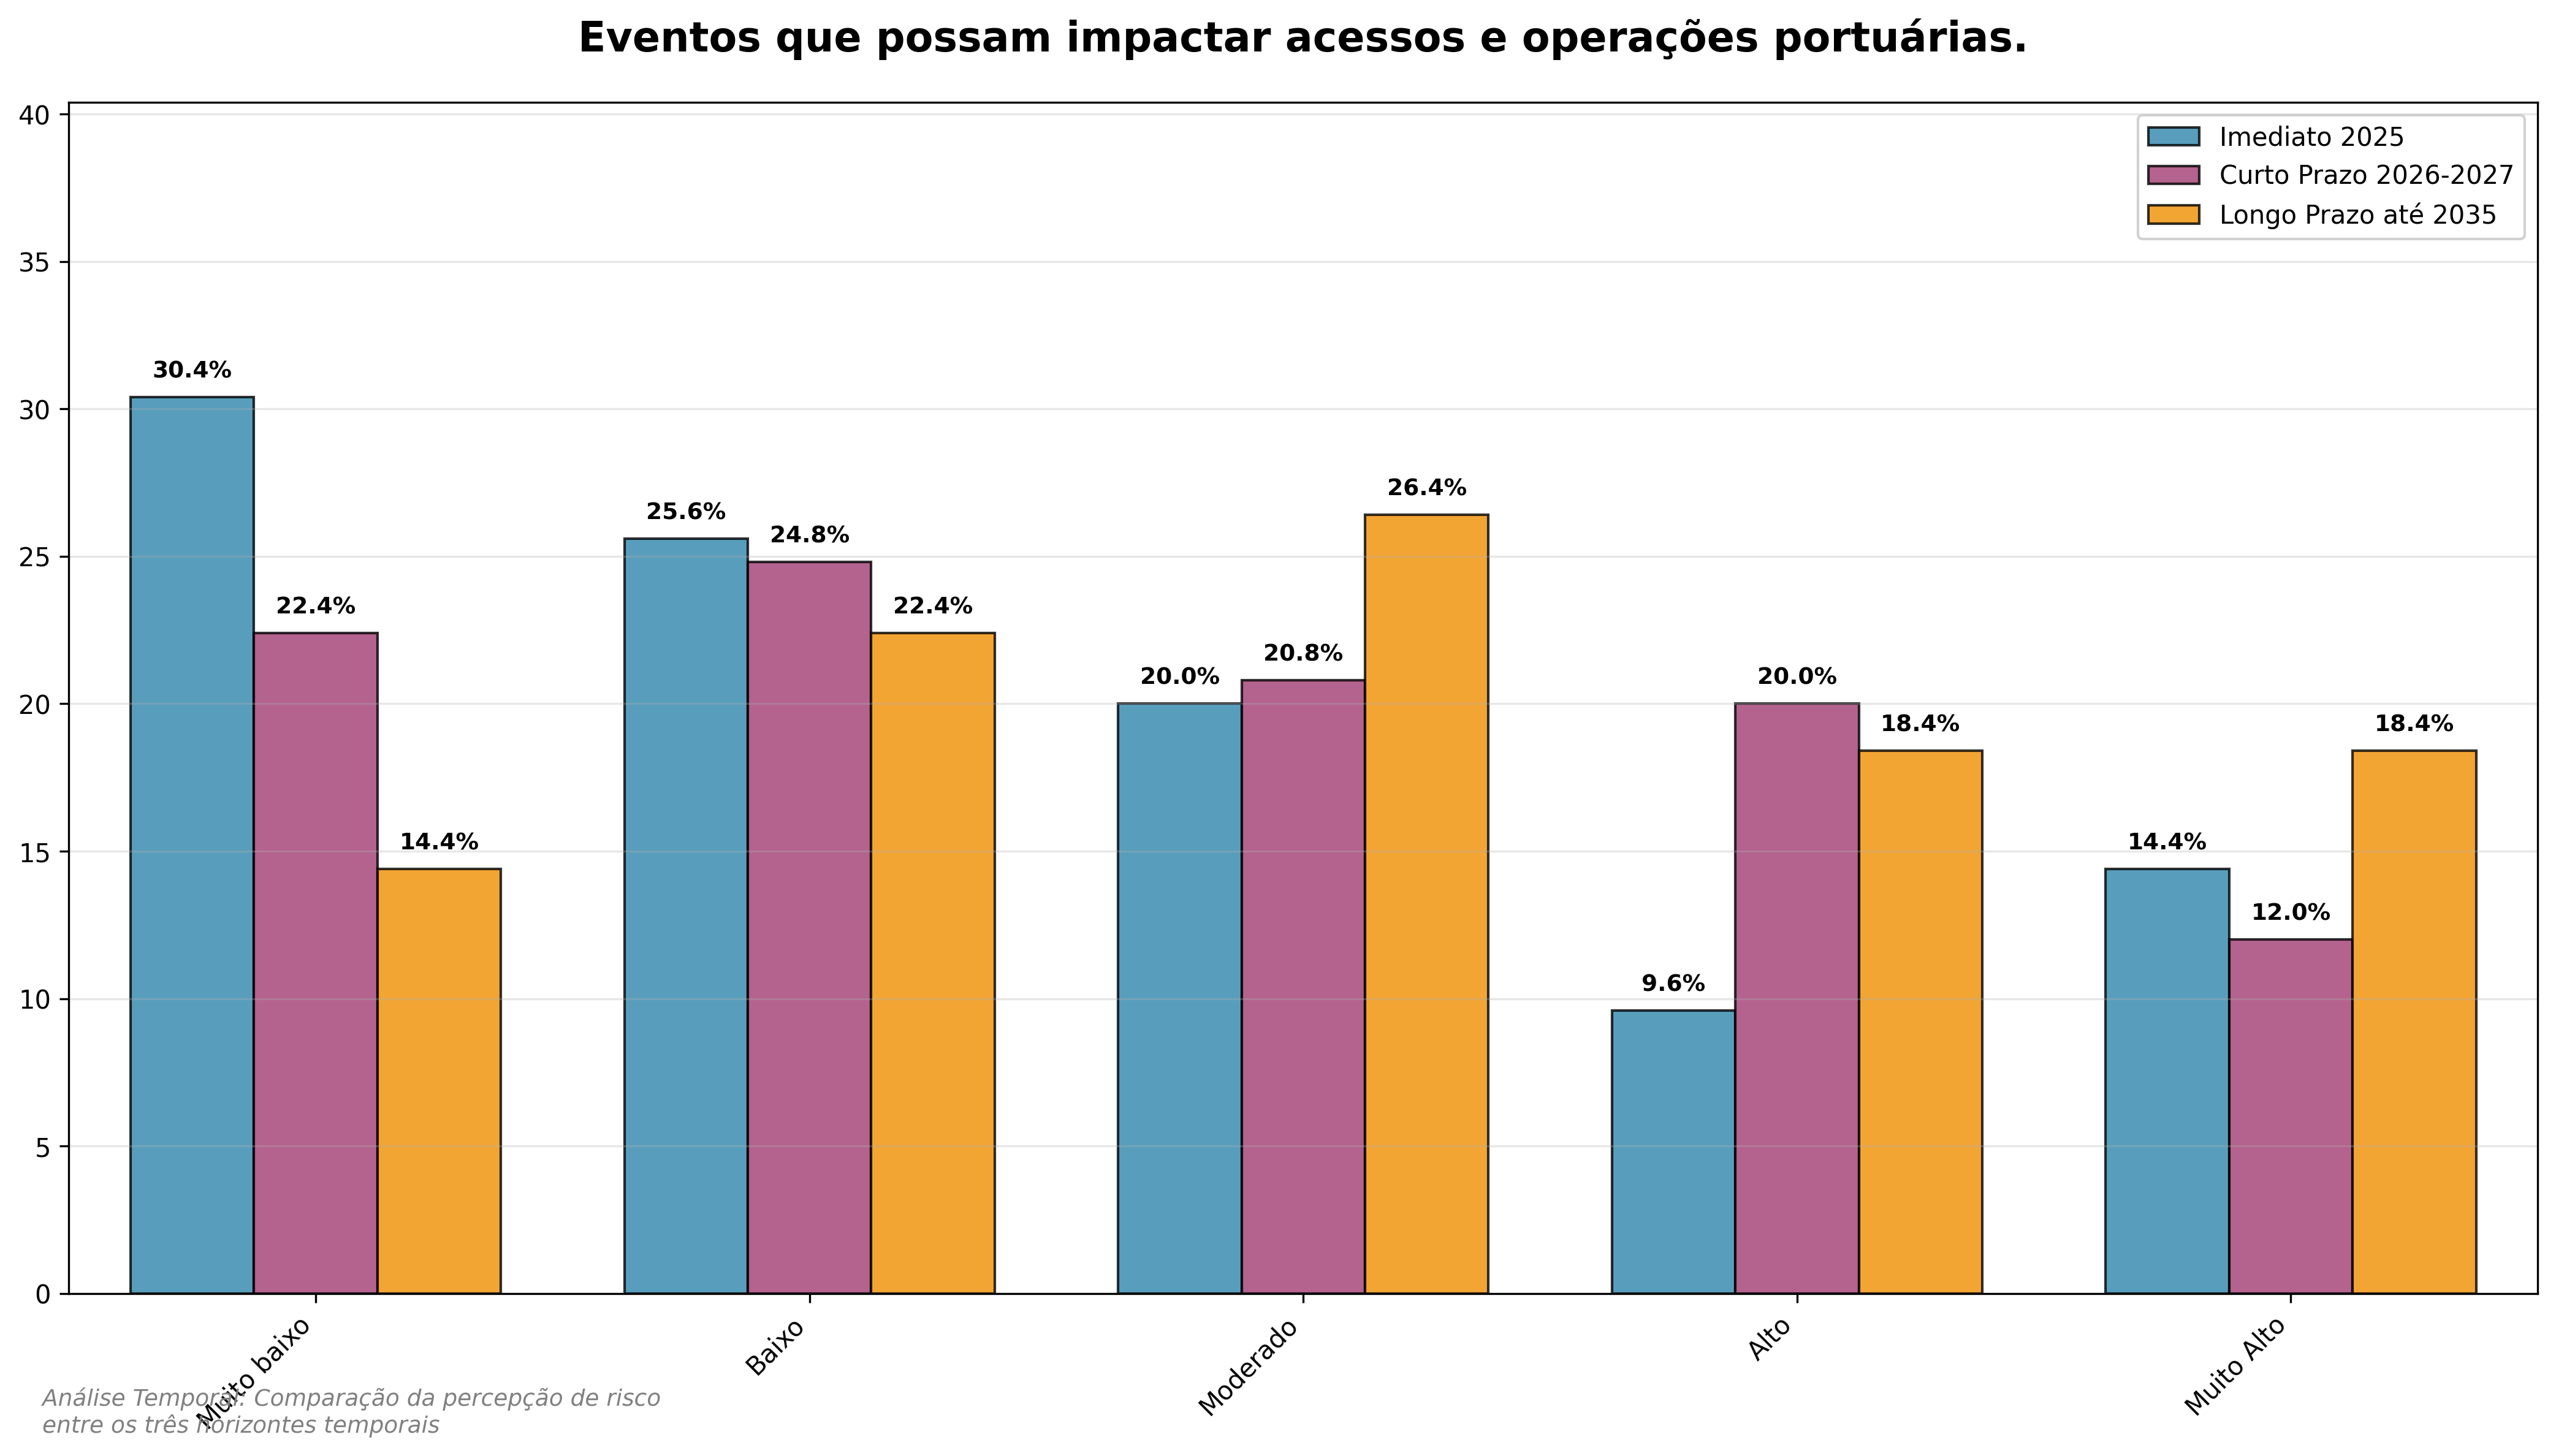
\includegraphics[keepaspectratio]{assets/ambientais/grafico_agrupado_2_2_temporal.png}}

\begin{tcolorbox}[enhanced jigsaw, titlerule=0mm, colback=white, title=\textcolor{quarto-callout-tip-color}{\faLightbulb}\hspace{0.5em}{Destaques}, opacityback=0, colbacktitle=quarto-callout-tip-color!10!white, leftrule=.75mm, left=2mm, colframe=quarto-callout-tip-color-frame, bottomrule=.15mm, bottomtitle=1mm, breakable, toprule=.15mm, toptitle=1mm, opacitybacktitle=0.6, arc=.35mm, coltitle=black, rightrule=.15mm]

\textbf{Evolução da Percepção de Risco}: A percepção de risco associada
à ocorrência de eventos climáticos extremos que possam impactar as
operações portuárias tende a aumentar progressivamente ao longo do
tempo.

\textbf{Contexto Detalhado por Período:}

\textbf{Período Imediato (2025):} Predomina a percepção de baixo risco,
com apenas 24\% dos respondentes avaliando os níveis alto (4) ou muito
alto (5) e mediana igual a 2.

\textbf{Curto Prazo (2026--2027):} Observa-se aumento gradual da
preocupação, com 32\% das respostas concentradas nos níveis 4-5, e
mediana de 3, sinalizando a expectativa de maior recorrência de eventos
disruptivos em curto prazo.

\textbf{Longo Prazo (até 2035):} A percepção de risco se intensifica,
atingindo 37\% dos respondentes nos níveis alto (4) e muito alto (5),
com mediana mantida em 3.

\textbf{Implicações Estratégicas:} Os eventos climáticos extremos, como
secas, enchentes, chuvas intensas e tempestades podem expor a
infraestrutura portuária a danos estruturais, falhas no fornecimento de
energia e interrupções em serviços essenciais. Essas condições podem
resultar em paralisação total ou parcial das operações, elevação dos
custos de manutenção e aumento dos riscos ocupacionais, comprometendo a
resiliência climática do empreendimento portuário e sua capacidade de
assegurar a continuidade operacional diante de cenários climáticos cada
vez mais extremos.

\end{tcolorbox}

\subsection{Mudanças climáticas (intensificação e aumento da frequência
de fenômenos
relacionados)}\label{mudanuxe7as-climuxe1ticas-intensificauxe7uxe3o-e-aumento-da-frequuxeancia-de-fenuxf4menos-relacionados}

O gr?fico a seguir apresenta a evolu??o temporal do risco Mudanças
climáticas (intensificação e aumento da frequência de fenômenos
relacionados).
\pandocbounded{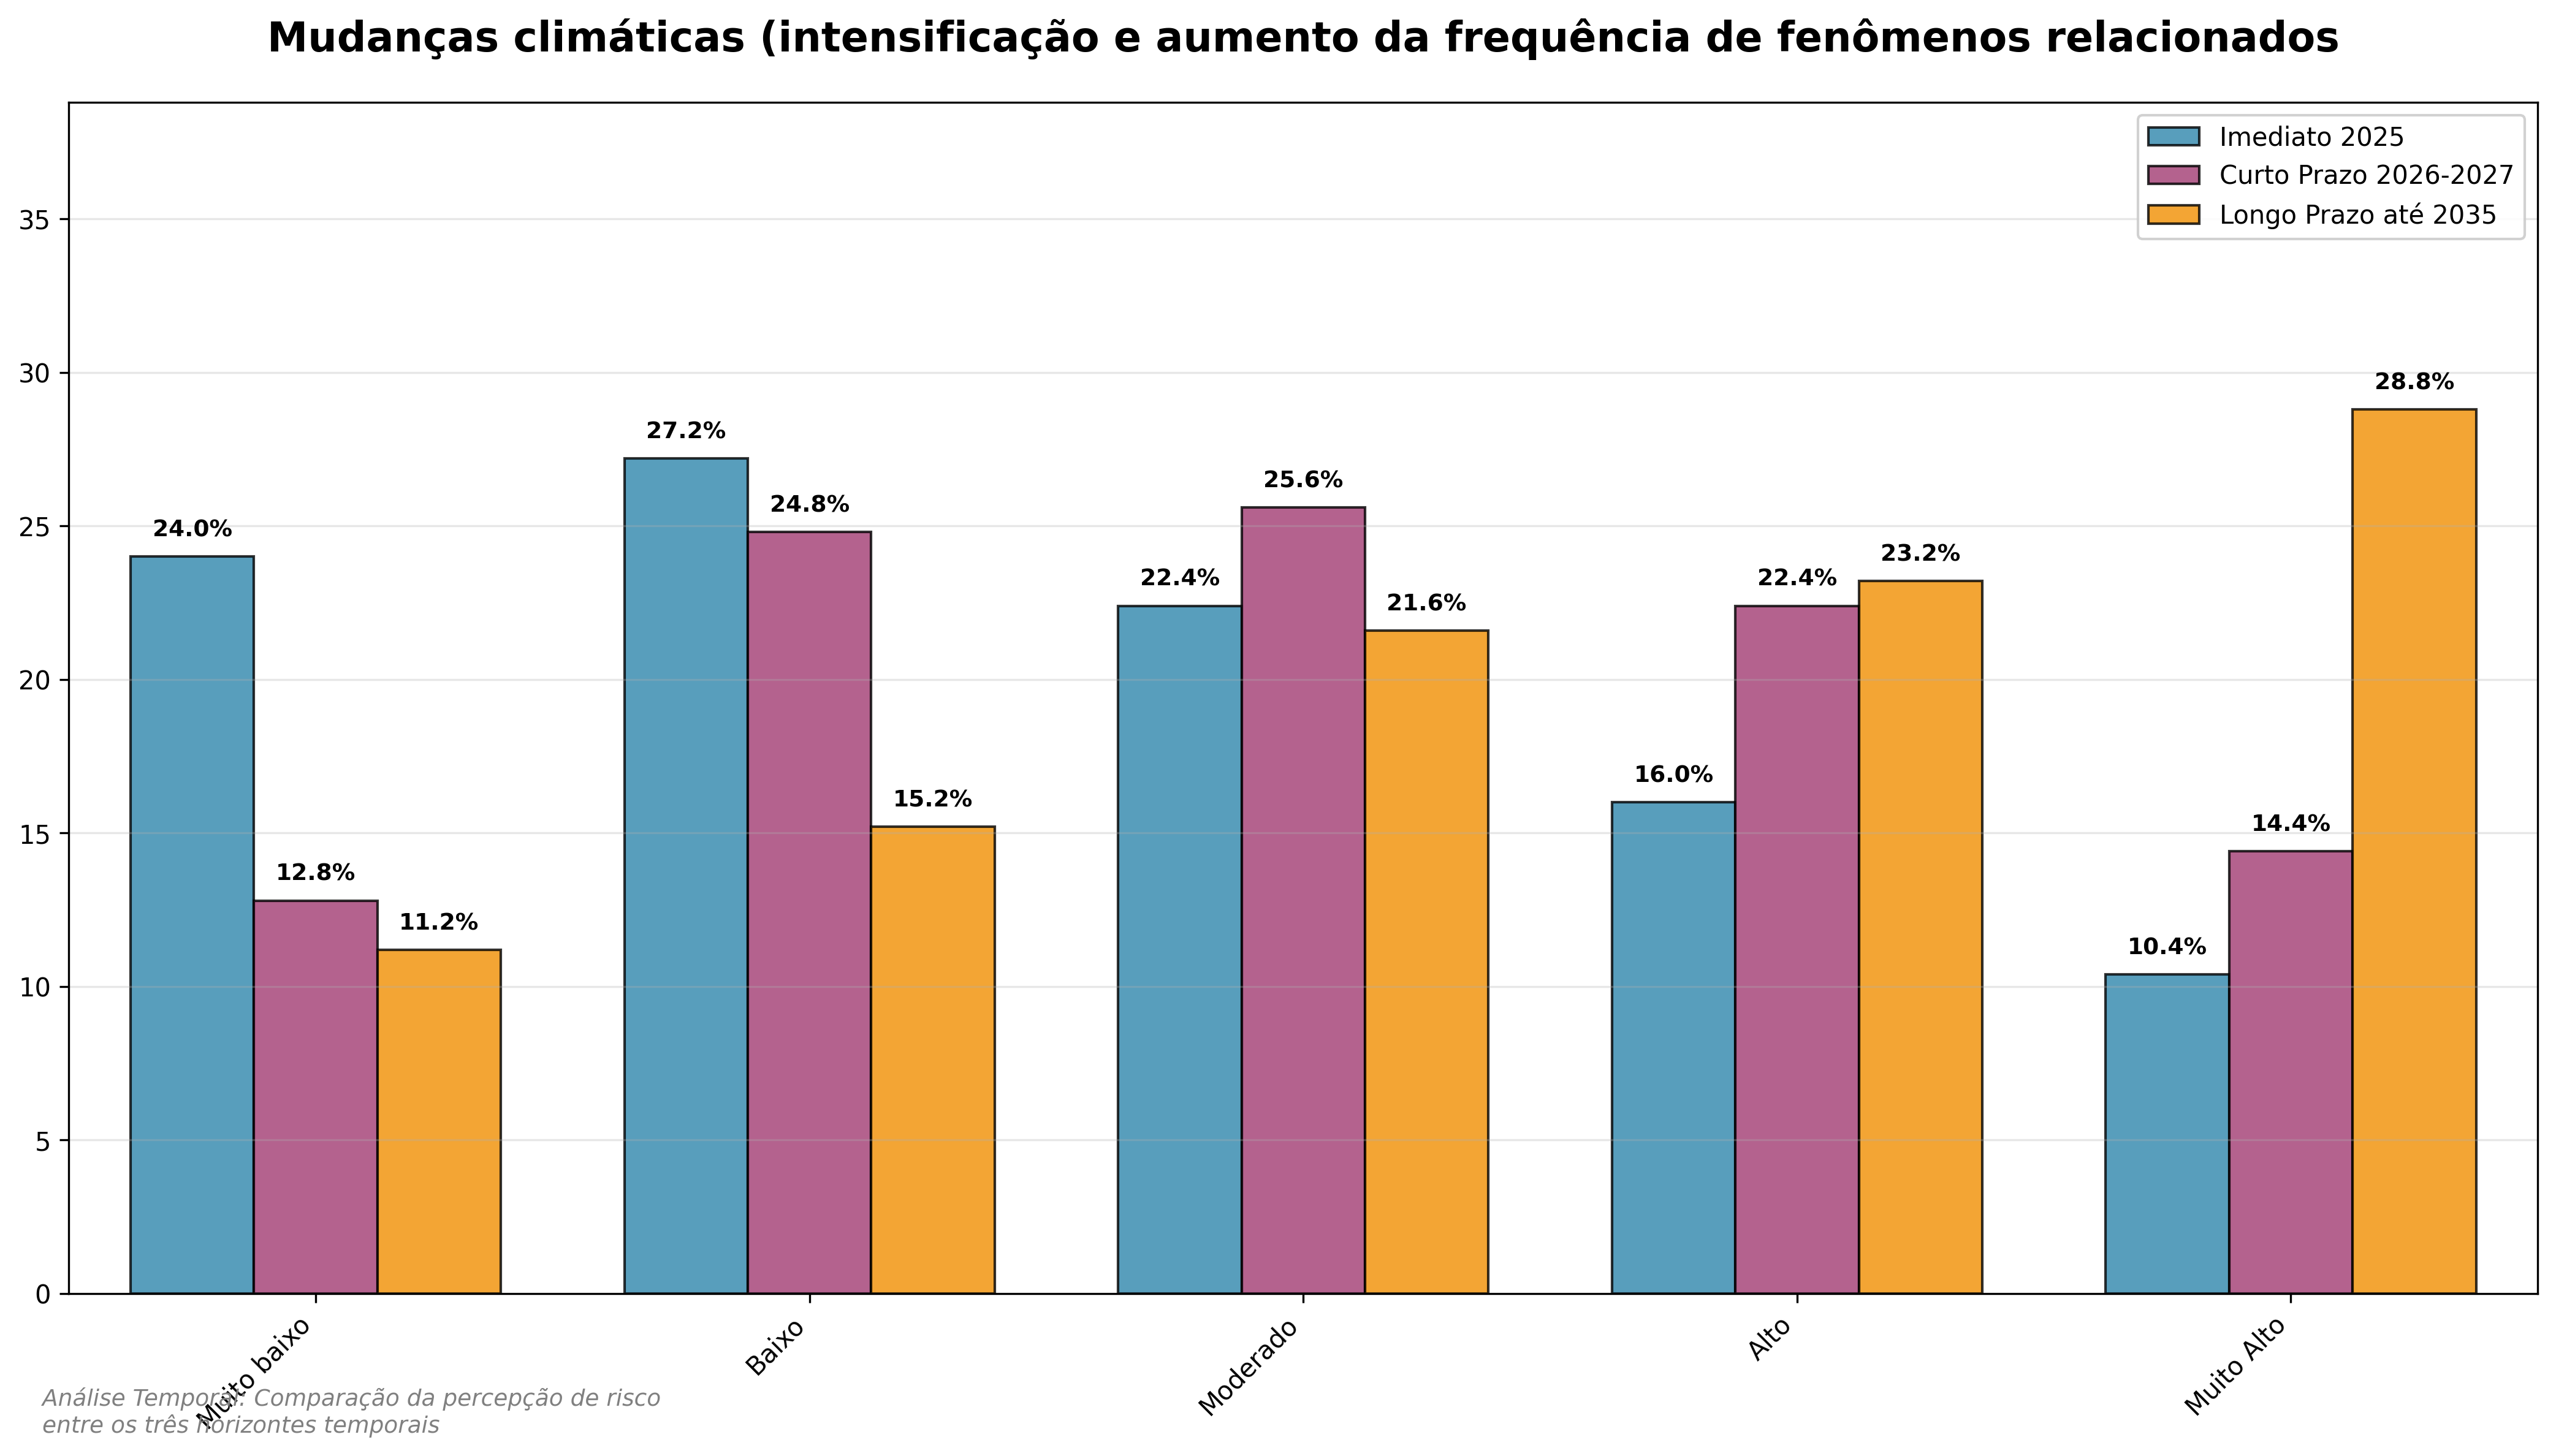
\includegraphics[keepaspectratio]{assets/ambientais/grafico_agrupado_2_3_temporal.png}}

\begin{tcolorbox}[enhanced jigsaw, titlerule=0mm, colback=white, title=\textcolor{quarto-callout-tip-color}{\faLightbulb}\hspace{0.5em}{Destaques}, opacityback=0, colbacktitle=quarto-callout-tip-color!10!white, leftrule=.75mm, left=2mm, colframe=quarto-callout-tip-color-frame, bottomrule=.15mm, bottomtitle=1mm, breakable, toprule=.15mm, toptitle=1mm, opacitybacktitle=0.6, arc=.35mm, coltitle=black, rightrule=.15mm]

\textbf{Evolução da Percepção de Risco:} Há uma tendência clara de
aumento progressivo na percepção de risco associada ao aquecimento
global e à intensificação das ondas de calor, refletindo a crescente
preocupação com seus efeitos sobre as operações portuárias e a
infraestrutura crítica. Esse padrão reflete a expectativa de que o
aquecimento global e os eventos de calor extremo se tornem mais
frequentes e intensos, exigindo planejamento adaptativo e medidas de
mitigação mais robustas.

\textbf{Contexto Detalhado por Período:}

\textbf{Período Imediato (2025):} A percepção de risco é moderada, com
26\% dos respondentes classificando o risco como alto (4) ou muito alto
(5), e mediana igual a 2, indicando que, no curto horizonte, o impacto
do aumento da temperatura ainda é percebido de forma limitada e
localizada.

\textbf{Curto Prazo (2026--2027):} Observa-se elevação significativa da
preocupação, com 37\% das respostas situadas nos níveis alto ou muito
alto, e mediana de 3, o que revela maior conscientização sobre os
efeitos das ondas de calor na produtividade, no bem-estar dos
trabalhadores e na eficiência operacional.

\textbf{Longo Prazo (até 2035):} A percepção de risco atinge seu nível
máximo, com 52\% dos respondentes apontando risco alto ou muito alto, e
mediana de 4, demonstrando reconhecimento do agravamento dos impactos do
aumento da temperatura média sobre a resiliência térmica das
infraestruturas e a segurança das atividades portuárias.

\textbf{Implicações Estratégicas:} O aumento da temperatura média e a
ocorrência de ondas de calor mais intensas e prolongadas podem provocar
sobreaquecimento de equipamentos, redução da eficiência energética,
danos à infraestrutura, e maior risco ocupacional para trabalhadores
expostos. Essas condições podem resultar em interrupções operacionais,
elevação dos custos de manutenção e climatização, e impactos diretos na
saúde e segurança das equipes portuárias, comprometendo a resiliência
climática e a continuidade das operações. Dessa forma, é essencial que
os portos adotem planos de adaptação climática, como melhorias na
ventilação e isolamento térmico, uso de materiais resistentes ao calor,
ajuste dos turnos de trabalho e monitoramento em tempo real de
temperaturas críticas, visando garantir a segurança operacional e a
eficiência energética em cenários de aquecimento global crescente.

\end{tcolorbox}

\subsection{Crise na disponibilidade de recursos naturais (água e
produção de
alimentos)}\label{crise-na-disponibilidade-de-recursos-naturais-uxe1gua-e-produuxe7uxe3o-de-alimentos}

O gr?fico a seguir apresenta a evolu??o temporal do risco Crise na
disponibilidade de recursos naturais (água e produção de alimentos).
\pandocbounded{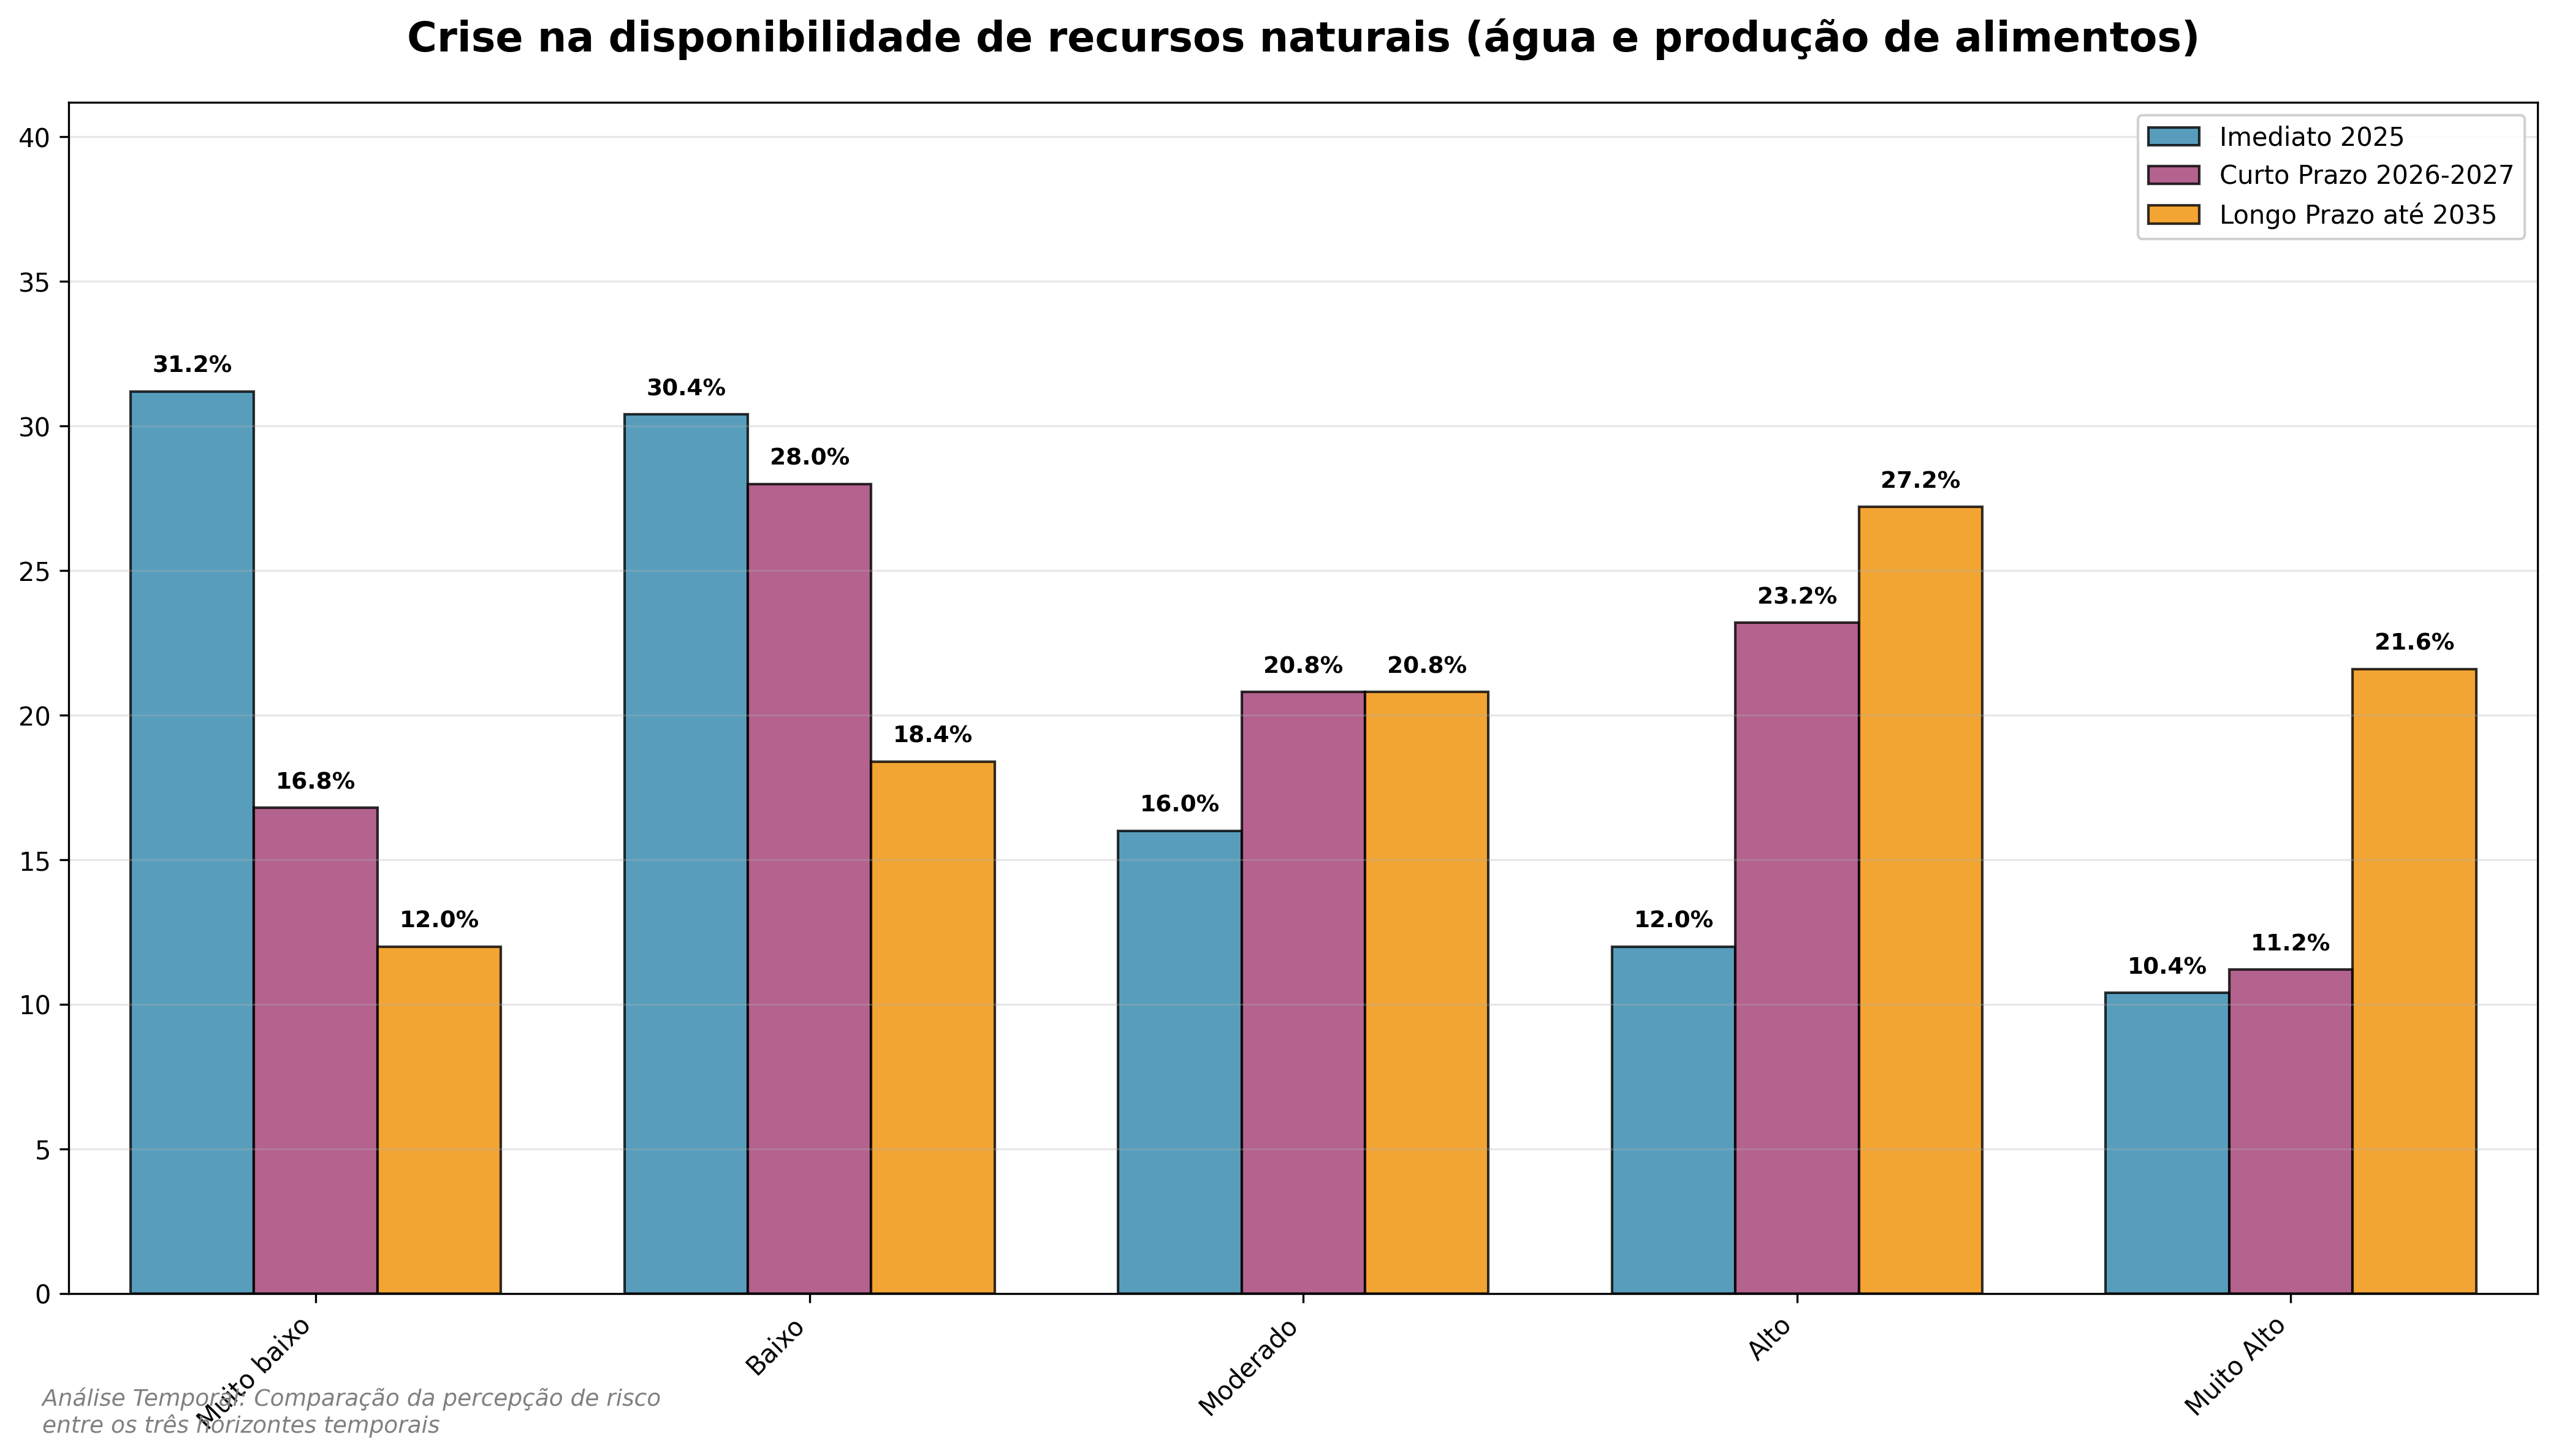
\includegraphics[keepaspectratio]{assets/ambientais/grafico_agrupado_2_4_temporal.png}}

\begin{tcolorbox}[enhanced jigsaw, titlerule=0mm, colback=white, title=\textcolor{quarto-callout-tip-color}{\faLightbulb}\hspace{0.5em}{Destaques}, opacityback=0, colbacktitle=quarto-callout-tip-color!10!white, leftrule=.75mm, left=2mm, colframe=quarto-callout-tip-color-frame, bottomrule=.15mm, bottomtitle=1mm, breakable, toprule=.15mm, toptitle=1mm, opacitybacktitle=0.6, arc=.35mm, coltitle=black, rightrule=.15mm]

\textbf{Evolução da Percepção de Risco:} A escassez de água e alimentos
deixa de ser considerada um risco periférico e consolida tendência de
deterioração: o percentual em níveis 4-5 cresce de 22\% para 49\% entre
2025 e 2035, enquanto o grupo que via o risco como baixo cai de 62\%
para 30\%.

\textbf{Contexto Detalhado por Período:}

\textbf{Período Imediato (2025):} Mediana em 2 e 22\% das respostas nos
níveis altos indicam atenção moderada, com maioria (62\%) ainda
percebendo disponibilidade aceitável de recursos críticos para
abastecimento portuário.

\textbf{Curto Prazo (2026-2027):} A mediana sobe para 3 e o risco alto
avança para 34\%, refletindo alerta sobre pressões em sistemas hídricos
regionais e cadeias agroindustriais que sustentam trabalhadores e
hinterlândias.

\textbf{Longo Prazo (até 2035):} O risco entra em patamar estrutural,
com 49\% das respostas nos níveis 4-5, mediana 3 e redução do grupo de
baixo risco para 30\%, sinalizando disputas crescentes por recursos
essenciais.

\textbf{Implicações Estratégicas:} A redução na disponibilidade de água
e alimentos pode gerar paralisações sanitárias, aumento de custos
operacionais e conflitos socioambientais nas áreas de influência dos
portos. Antecipar-se requer planos de uso eficiente da água,
diversificação de fornecedores de suprimentos críticos, programas de
apoio alimentar às comunidades portuárias e participação ativa em
agendas de segurança hídrica e alimentar regionais.

\end{tcolorbox}

\subsection{Desastres naturais não relacionados ao clima, como
terremotos, incêndios florestais, maremotos,
subsidência}\label{desastres-naturais-nuxe3o-relacionados-ao-clima-como-terremotos-incuxeandios-florestais-maremotos-subsiduxeancia}

O gr?fico a seguir apresenta a evolu??o temporal do risco Desastres
naturais não relacionados ao clima, como terremotos, incêndios
florestais, maremotos, subsidência.
\pandocbounded{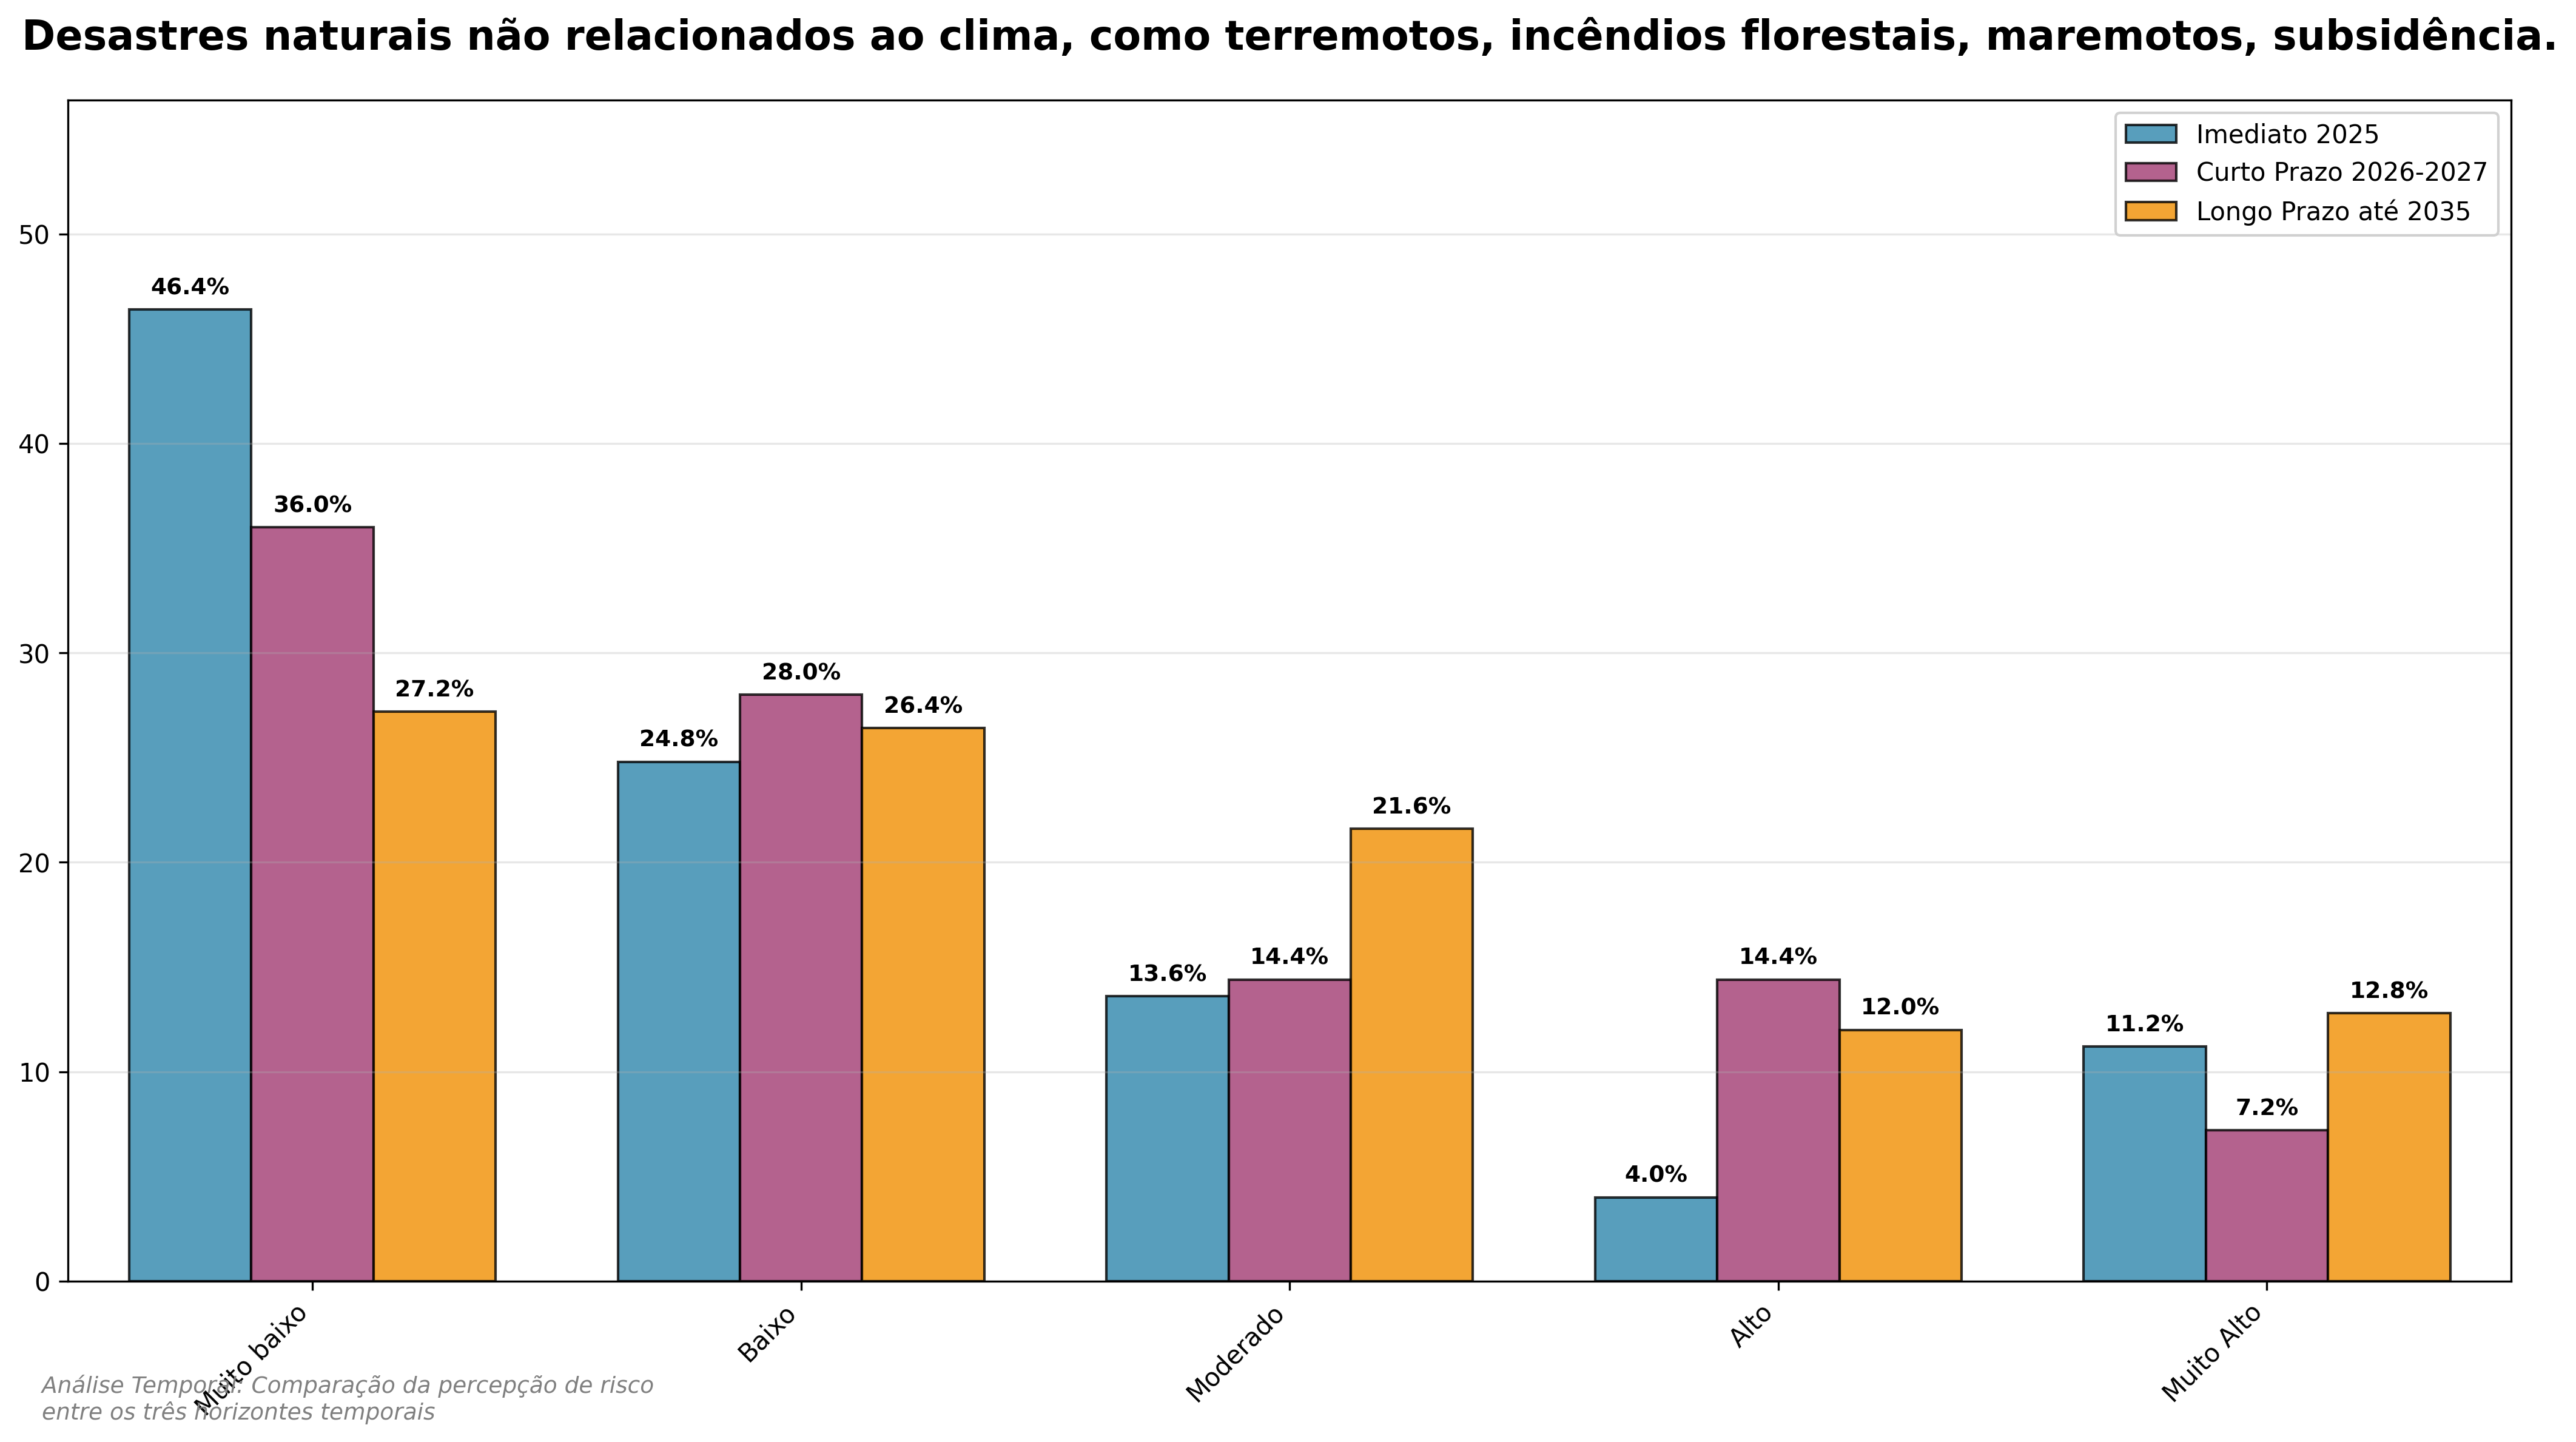
\includegraphics[keepaspectratio]{assets/ambientais/grafico_agrupado_2_5_temporal.png}}

\begin{tcolorbox}[enhanced jigsaw, titlerule=0mm, colback=white, title=\textcolor{quarto-callout-tip-color}{\faLightbulb}\hspace{0.5em}{Destaques}, opacityback=0, colbacktitle=quarto-callout-tip-color!10!white, leftrule=.75mm, left=2mm, colframe=quarto-callout-tip-color-frame, bottomrule=.15mm, bottomtitle=1mm, breakable, toprule=.15mm, toptitle=1mm, opacitybacktitle=0.6, arc=.35mm, coltitle=black, rightrule=.15mm]

\textbf{Evolução da Percepção de Risco:} Os dados mostram uma tendência
de aumento da percepção de risco associada à ocorrência de desastres
naturais não relacionados ao clima, como terremotos, incêndios
florestais, maremotos e processos de subsidência. Embora a maioria dos
respondentes ainda perceba tais eventos como de baixo risco, há uma
pequena mudança de percepção nos horizontes de curto e longo prazo.

\textbf{Contexto Detalhado por Período:}

\textbf{Período Imediato (2025):} Predomina uma percepção de baixo
risco, com apenas 15\% das respostas concentradas nos níveis alto (4) ou
muito alto (5), e mediana igual a 2, o que indica que tais eventos são
vistos como improváveis no curto horizonte.

\textbf{Curto Prazo (2026--2027):} Observa-se aumento gradual da
preocupação, com 22\% dos respondentes classificando o risco como alto
ou muito alto, e mediana de 3.

\textbf{Longo Prazo (até 2035):} A tendência de elevação da percepção de
risco se mantém, alcançando 25\% das respostas nos níveis 4 e 5.

\textbf{Implicações Estratégicas}: A ocorrência de desastres naturais
não relacionados ao clima, como terremotos, incêndios florestais,
maremotos e processos de subsidência, pode ocasionar danos estruturais
súbitos em píeres, armazéns, tanques de armazenamento e vias de acesso.
Esses eventos podem levar à interrupção imediata das operações
portuárias, elevação dos riscos de vazamentos, explosões e contaminações
ambientais, e comprometimento da integridade estrutural e da segurança
ambiental da área portuária. Assim, torna-se essencial o planejamento
preventivo, incluindo monitoramento geotécnico e sísmico, planos de
evacuação e contingência, e estratégias de resposta rápida, de modo a
mitigar os impactos e garantir a continuidade operacional em
emergências.

\end{tcolorbox}

\subsection{Aumento do nível do mar e processos erosivos
costeiros}\label{aumento-do-nuxedvel-do-mar-e-processos-erosivos-costeiros}

O gr?fico a seguir apresenta a evolu??o temporal do risco Aumento do
nível do mar e processos erosivos costeiros.
\pandocbounded{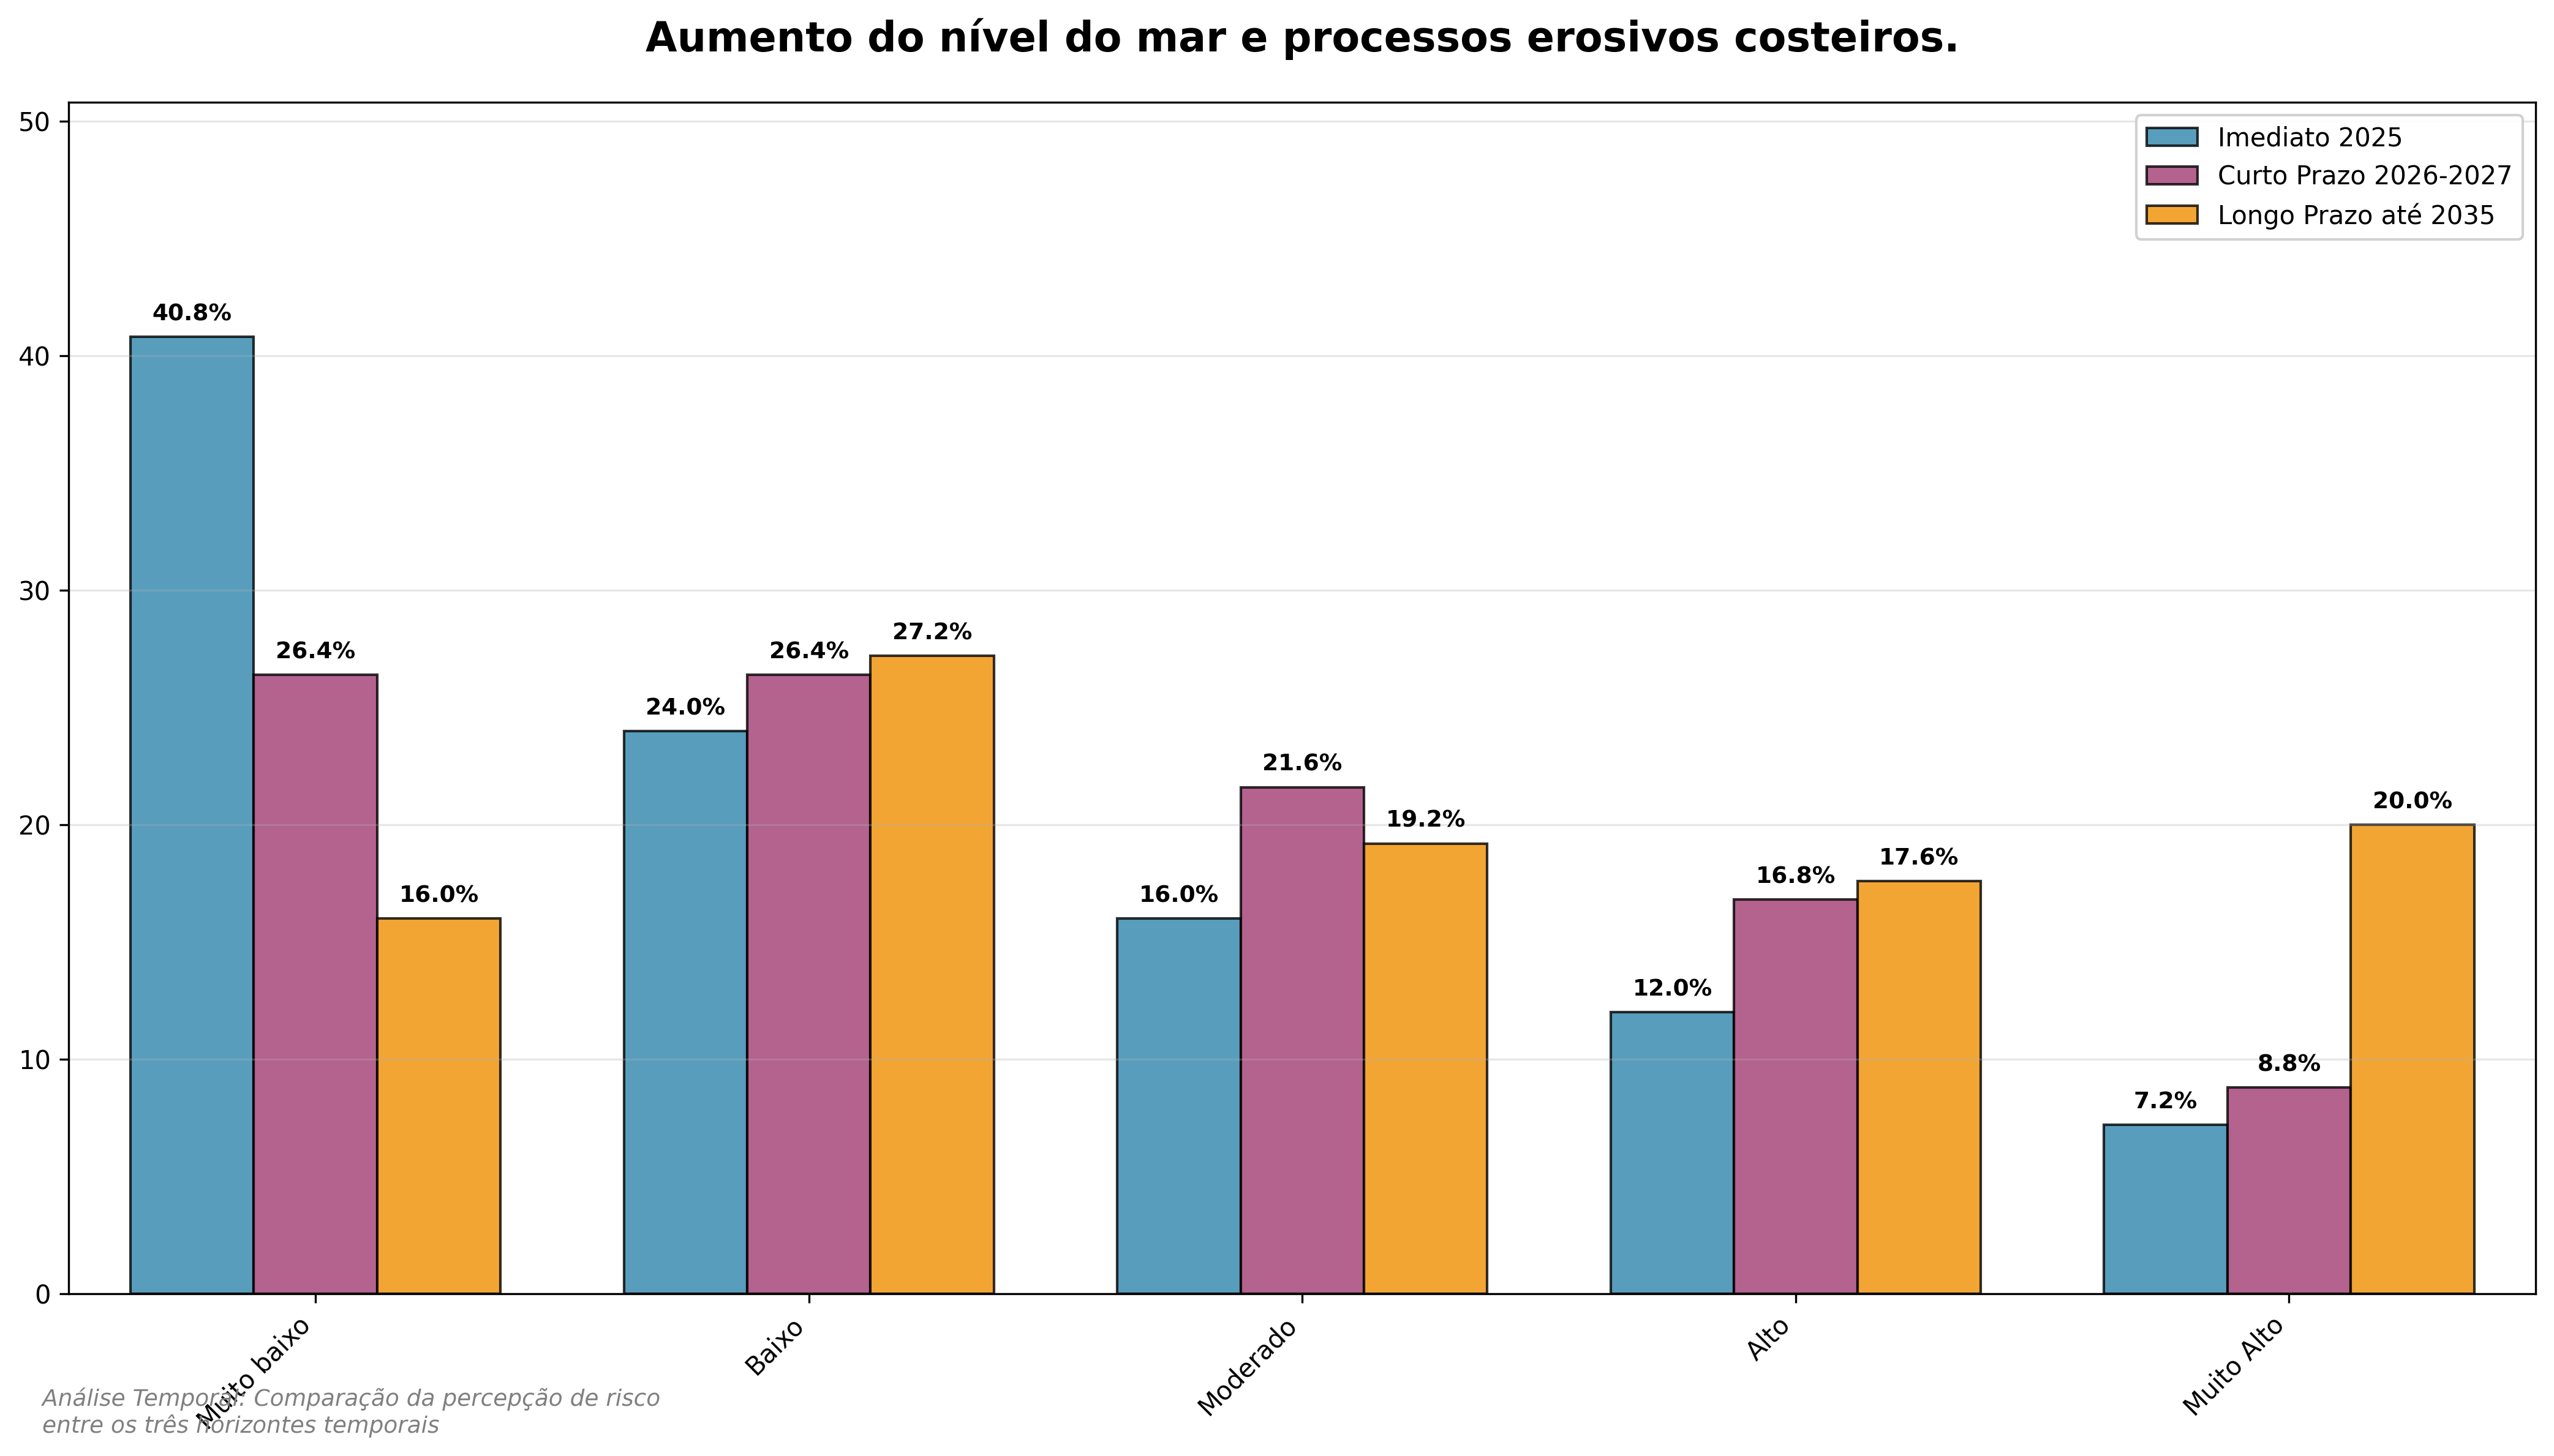
\includegraphics[keepaspectratio]{assets/ambientais/grafico_agrupado_2_6_temporal.png}}

\begin{tcolorbox}[enhanced jigsaw, titlerule=0mm, colback=white, title=\textcolor{quarto-callout-tip-color}{\faLightbulb}\hspace{0.5em}{Destaques}, opacityback=0, colbacktitle=quarto-callout-tip-color!10!white, leftrule=.75mm, left=2mm, colframe=quarto-callout-tip-color-frame, bottomrule=.15mm, bottomtitle=1mm, breakable, toprule=.15mm, toptitle=1mm, opacitybacktitle=0.6, arc=.35mm, coltitle=black, rightrule=.15mm]

\textbf{Evolução da Percepção de Risco:} o gráfico mostra uma tendência
clara de aumento da percepção de risco associada ao aumento do nível do
mar e aos processos erosivos costeiros, indicando que os respondentes
reconhecem de forma crescente os impactos estruturais e operacionais que
esses fenômenos podem provocar no ambiente portuário.

\textbf{totaContexto Detalhado por Período:}

\textbf{Período Imediato (2025):} predomina uma percepção de baixo
risco, com 19\% das respostas classificando o risco como alto (4) ou
muito alto (5) e mediana igual a 2, o que sugere que, no curto
horizonte, o aumento do nível do mar ainda é percebido como uma ameaça
distante ou de baixa frequência.

\textbf{Curto Prazo (2026--2027):} observa-se elevação gradual da
preocupação, com 26\% dos respondentes avaliando o risco como alto ou
muito alto, mantendo mediana em 2.

\textbf{Longo Prazo (até 2035):} a percepção de risco se intensifica
expressivamente, com 38\% das respostas concentradas nos níveis alto (4)
e muito alto (5), e mediana de 3, evidenciando reconhecimento crescente
da vulnerabilidade dos portos diante da elevação do nível do mar e da
erosão costeira.

\textbf{Implicações Estratégicas:} o aumento do nível do mar e a
intensificação dos processos erosivos costeiros podem ocasionar perda
gradual de áreas operacionais e instabilidade estrutural em cais,
quebra-mares, taludes e vias de acesso. Essas condições demandam a
intensificação das manutenções preventivas, investimentos emergenciais
em obras de contenção e proteção costeira, em casos críticos, a
relocalização de ativos estratégicos. Tais medidas, embora necessárias,
podem comprometer o planejamento de longo prazo e a viabilidade
econômica da infraestrutura portuária, tornando imprescindível o
monitoramento contínuo das variações do nível do mar, o uso de
modelagens hidrodinâmicas preditivas e a adoção de soluções baseadas na
natureza para mitigar os efeitos erosivos e garantir a resiliência
costeira e operacional dos portos.

\end{tcolorbox}

\subsection{Poluição da água e sedimentos em áreas portuárias por
contaminantes orgânicos e inorgânicos, tais como hidrocarbonetos,
metais, pesticidas e
nutrientes}\label{poluiuxe7uxe3o-da-uxe1gua-e-sedimentos-em-uxe1reas-portuuxe1rias-por-contaminantes-orguxe2nicos-e-inorguxe2nicos-tais-como-hidrocarbonetos-metais-pesticidas-e-nutrientes}

O gr?fico a seguir apresenta a evolu??o temporal do risco Poluição da
água e sedimentos em áreas portuárias por contaminantes orgânicos e
inorgânicos, tais como hidrocarbonetos, metais, pesticidas e nutrientes.
\pandocbounded{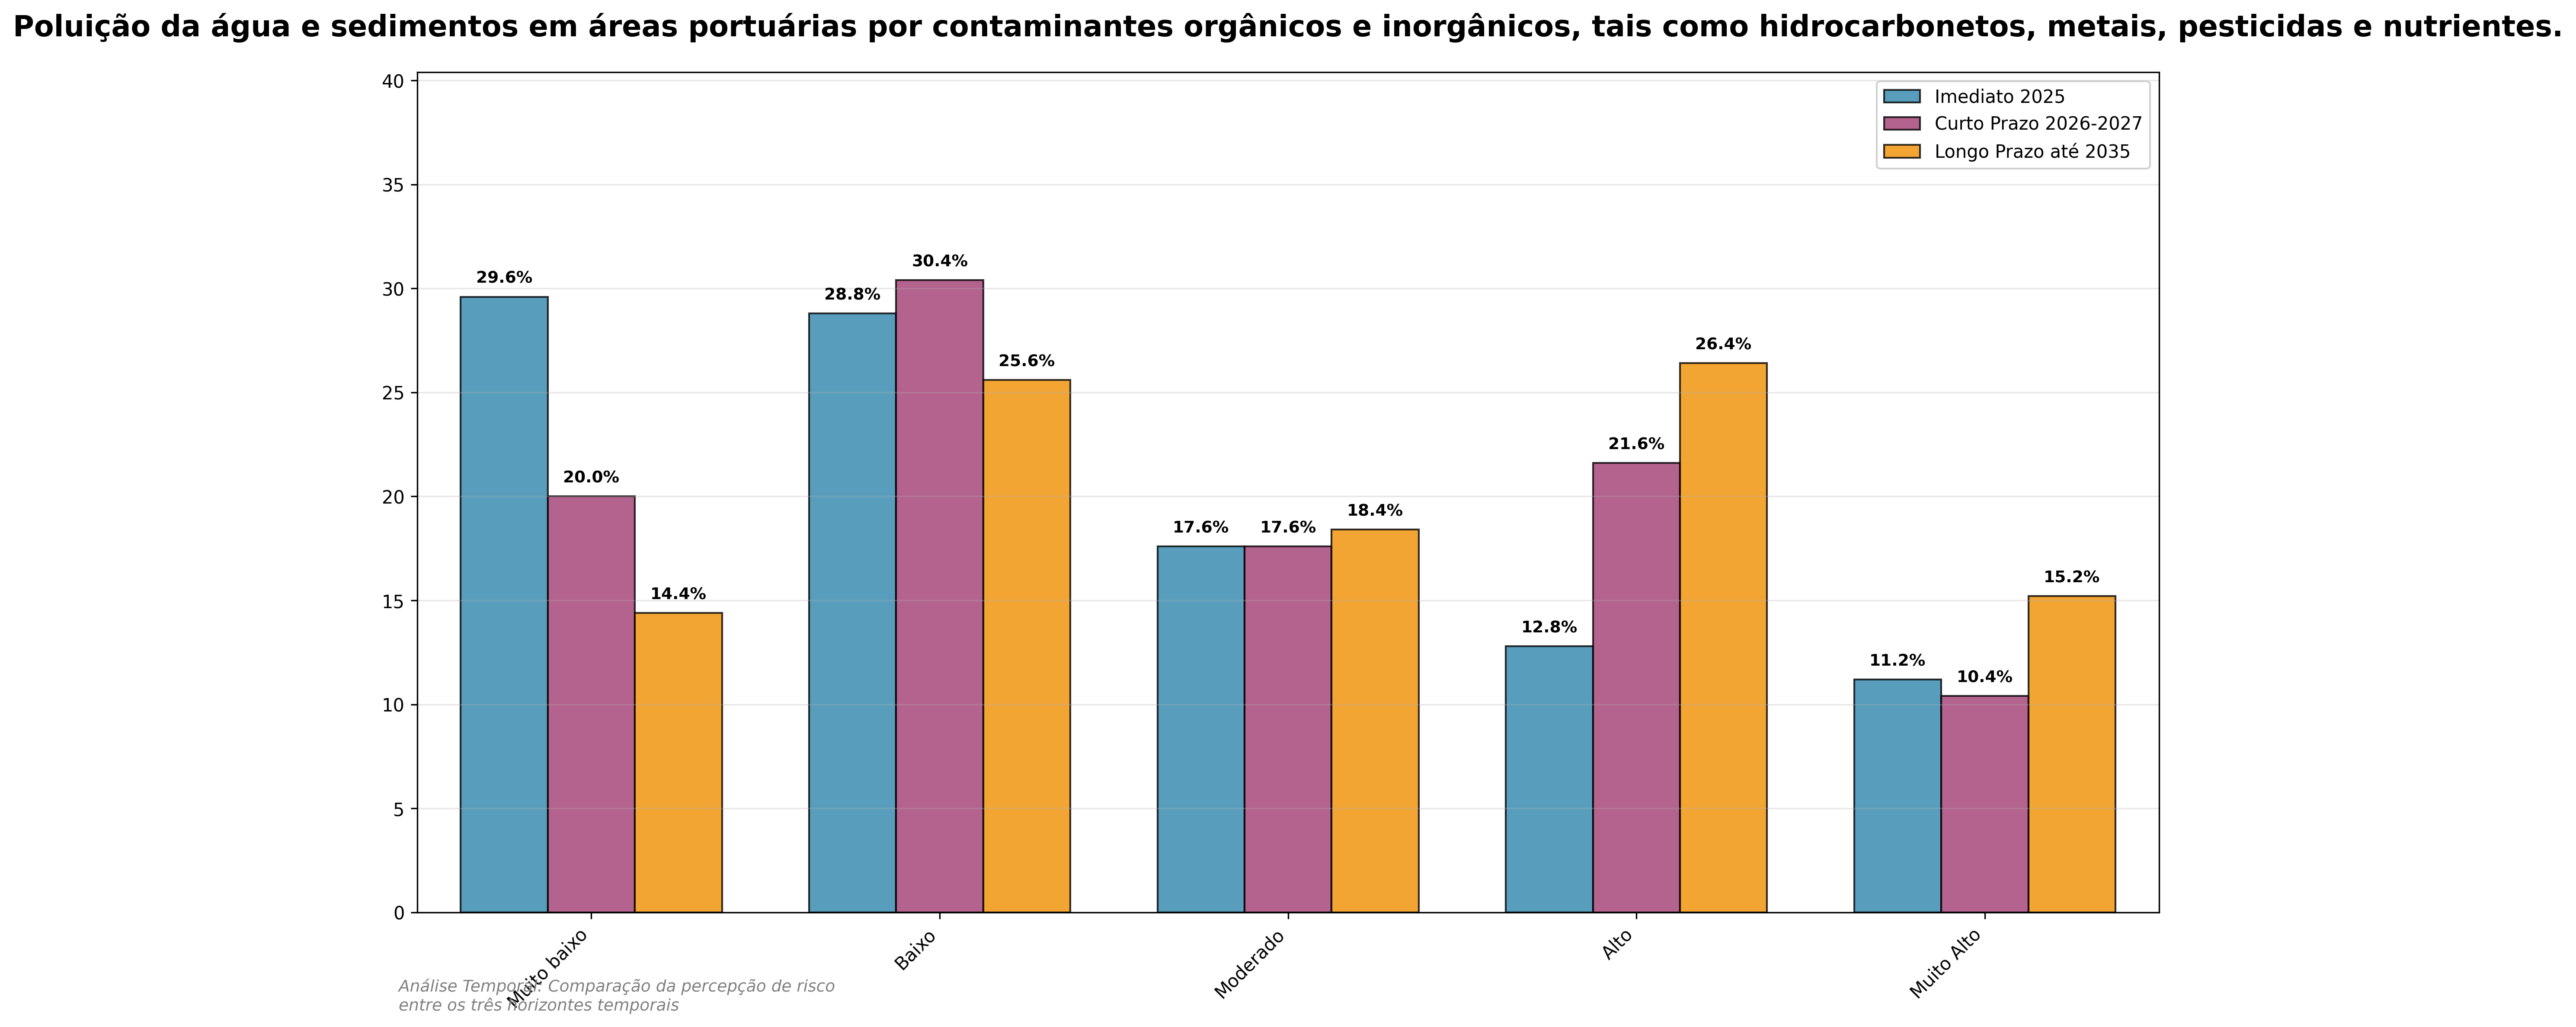
\includegraphics[keepaspectratio]{assets/ambientais/grafico_agrupado_2_7_temporal.png}}

\begin{tcolorbox}[enhanced jigsaw, titlerule=0mm, colback=white, title=\textcolor{quarto-callout-tip-color}{\faLightbulb}\hspace{0.5em}{Destaques}, opacityback=0, colbacktitle=quarto-callout-tip-color!10!white, leftrule=.75mm, left=2mm, colframe=quarto-callout-tip-color-frame, bottomrule=.15mm, bottomtitle=1mm, breakable, toprule=.15mm, toptitle=1mm, opacitybacktitle=0.6, arc=.35mm, coltitle=black, rightrule=.15mm]

\textbf{Evolução da Percepção de Risco:} O gráfico indica uma tendência
de aumento gradual da percepção de risco relacionada à escassez de
recursos hídricos e à crise de abastecimento, refletindo o
reconhecimento crescente da importância da segurança hídrica para a
continuidade das operações portuárias e o bem-estar das comunidades
locais. \textbar{}\\
\textbf{Contexto Detalhado por Período:} \textbar{}\\
\textbf{Período Imediato (2025):} A percepção de risco é ainda moderada,
com 24\% das respostas classificando o risco como alto (4) ou muito alto
(5), e mediana igual a 2, o que sugere que, no curto prazo, a maioria
dos respondentes não considera a escassez hídrica uma ameaça imediata à
operação portuária. \textbar{}\\
\textbf{Curto Prazo (2026--2027):} Observa-se aumento significativo da
preocupação, com 32\% das respostas concentradas nos níveis alto ou
muito alto, mantendo mediana em 2, indicando maior percepção sobre
possíveis restrições no abastecimento de água e seus impactos sobre a
eficiência operacional. \textbar{}\\
\textbf{Longo Prazo (até 2035):} A percepção de risco se intensifica de
forma expressiva, com 42\% dos respondentes avaliando o risco como alto
(4) ou muito alto (5) e mediana de 3, revelando expectativa de
agravamento da crise hídrica e de seus efeitos sobre as atividades
industriais, logísticas e sociais no entorno portuário. \textbar{}\\
\textbf{Implicações Estratégicas:} A escassez de recursos hídricos e a
crise de abastecimento podem gerar limitações no fornecimento de água
para uso industrial, sanitário e de suporte às tripulações, além de
provocar pressões adicionais sobre as cadeias logísticas de suprimento
de alimentos e insumos. Tais condições podem exigir a adoção de medidas
de racionamento interno, aumento dos custos operacionais e tensões
sociais com as comunidades vizinhas, comprometendo a segurança hídrica e
o relacionamento socioambiental do empreendimento portuário. Nesse
contexto, torna-se essencial implementar estratégias de gestão integrada
de recursos hídricos, como reúso e reciclagem de água, instalação de
sistemas de captação de águas pluviais, monitoramento de consumo em
tempo real e parcerias com autoridades locais para garantir o
abastecimento sustentável, fortalecendo a resiliência hídrica e a
sustentabilidade operacional dos portos. \textbar{}

\subsection{Movimentação de produtos
perigosos}\label{movimentauxe7uxe3o-de-produtos-perigosos}

\end{tcolorbox}

O gr?fico a seguir apresenta a evolu??o temporal do risco Movimentação
de produtos perigosos.
\pandocbounded{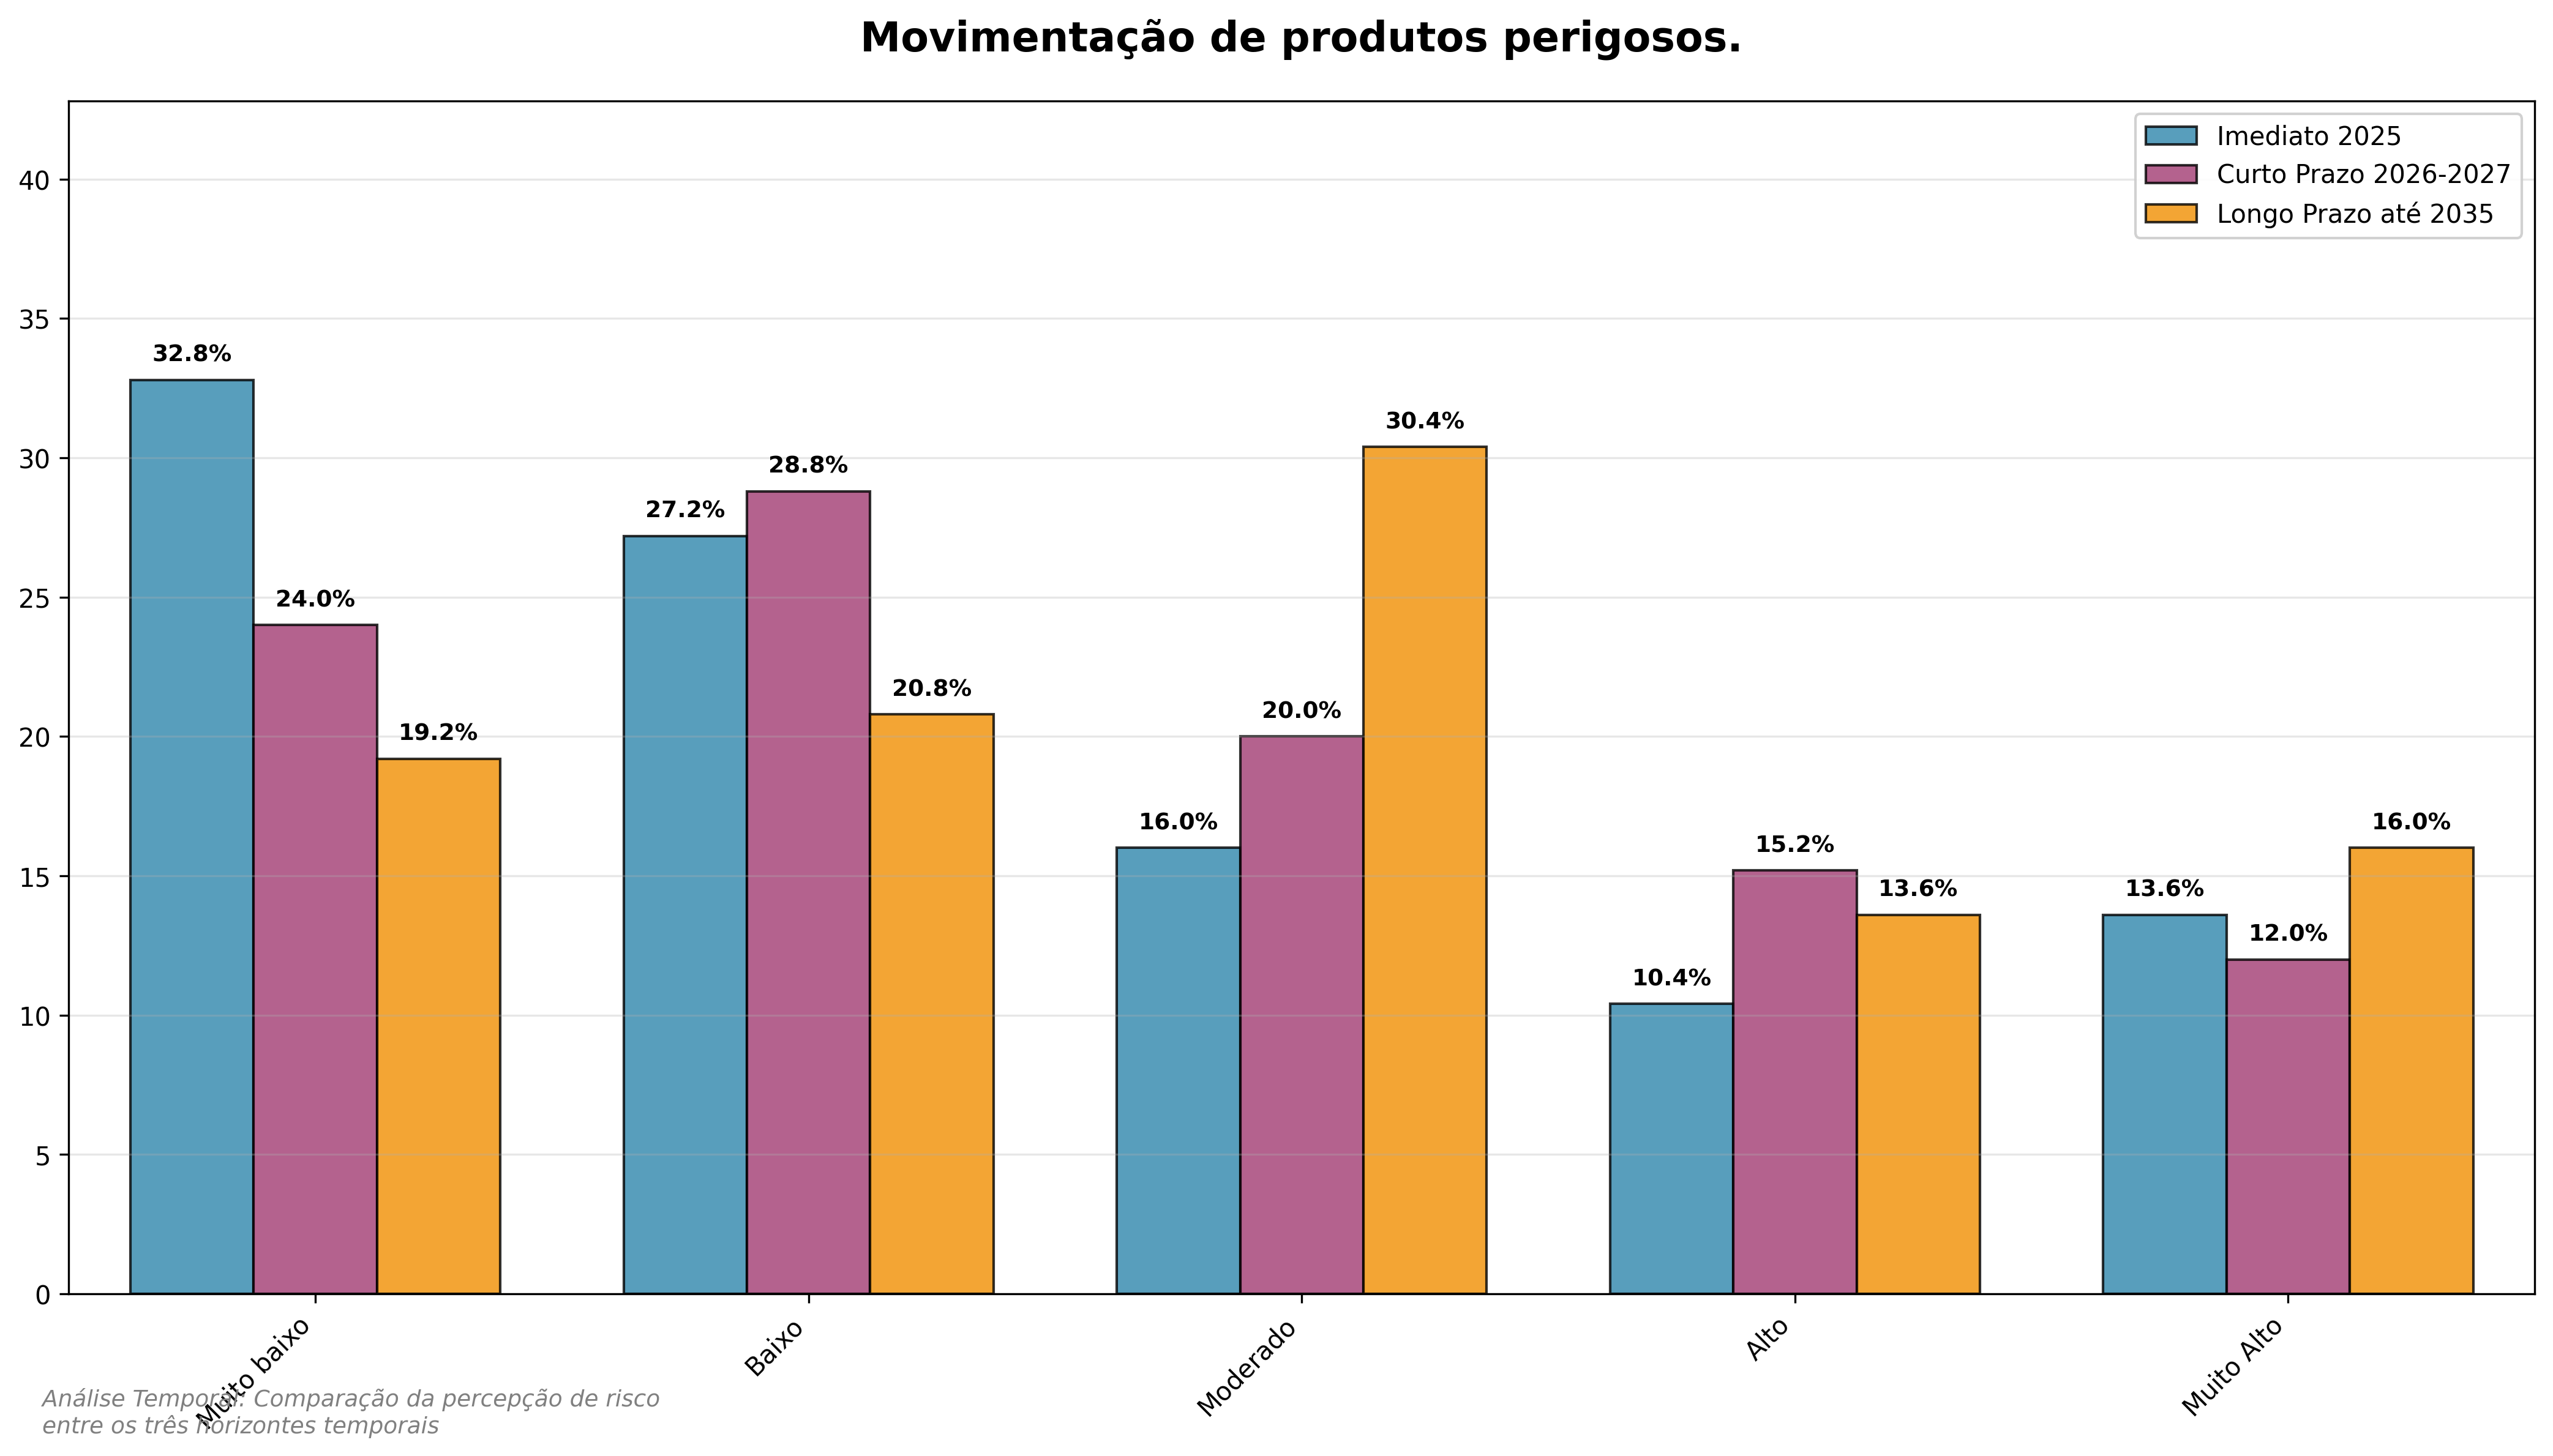
\includegraphics[keepaspectratio]{assets/ambientais/grafico_agrupado_2_8_temporal.png}}

\begin{tcolorbox}[enhanced jigsaw, titlerule=0mm, colback=white, title=\textcolor{quarto-callout-tip-color}{\faLightbulb}\hspace{0.5em}{Destaques}, opacityback=0, colbacktitle=quarto-callout-tip-color!10!white, leftrule=.75mm, left=2mm, colframe=quarto-callout-tip-color-frame, bottomrule=.15mm, bottomtitle=1mm, breakable, toprule=.15mm, toptitle=1mm, opacitybacktitle=0.6, arc=.35mm, coltitle=black, rightrule=.15mm]

\textbf{Evolução da Percepção de Risco:} O gráfico demonstra uma
tendência crescente de percepção de risco associada à introdução de
espécies exóticas invasoras, organismos aquáticos nocivos e agentes
patogênicos, fenômeno frequentemente vinculado à descarga de água de
lastro. Essa evolução sugere maior reconhecimento dos riscos ambientais
e regulatórios para o setor portuário.~

\textbf{Contexto Detalhado por Período:}

\textbf{Período Imediato (2025):} A percepção de risco é moderada, com
24\% das respostas classificando o risco como alto (4) ou muito alto
(5), e mediana igual a 2, indicando que, no horizonte mais próximo, os
impactos são percebidos como pontuais ou de baixa probabilidade.

\textbf{Curto Prazo (2026--2027):} Observa-se elevação gradual da
preocupação, com 27\% dos respondentes avaliando o risco como alto ou
muito alto, mantendo mediana em 2, refletindo maior atenção às
exigências regulatórias internacionais e à gestão de águas de lastro.

\textbf{Longo Prazo (até 2035):} A percepção de risco se intensifica
expressivamente, alcançando 35\% das respostas nos níveis alto (4) e
muito alto (5), e mediana igual a 3, evidenciando reconhecimento de que
a proliferação de espécies invasoras representa ameaça crescente à
biodiversidade marinha e às atividades portuárias.

\hfill\break
\textbf{Implicações Estratégica:} A introdução de espécies exóticas
invasoras, organismos aquáticos nocivos e agentes patogênicos, seja por
descarga de água de lastro ou outro tipo de descarte pode causar
desequilíbrios ecológicos graves, com competição entre espécies nativas
e invasoras, alteração de habitats e danos irreversíveis à
biodiversidade local. Essas ocorrências podem demandar ações corretivas
onerosas e restrições adicionais de atracação e manuseio de embarcações,
impactando diretamente a conformidade ambiental e a reputação
institucional do porto. Entre as medidas preventivas prioritárias
destacam-se: monitoramento e registro contínuo das operações de lastro,
adoção de tecnologias de tratamento de água de lastro a bordo e~
capacitação das equipes para resposta rápida a incidentes ambientais.
Essas ações são fundamentais para assegurar a conformidade com normas
internacionais, preservar os ecossistemas costeiros e fortalecer a
governança ambiental do complexo portuário.

\end{tcolorbox}

\subsection{Presença de agentes patogênicos (Deficiência no tratamento
de esgoto ou
saneamento)}\label{presenuxe7a-de-agentes-patoguxeanicos-deficiuxeancia-no-tratamento-de-esgoto-ou-saneamento}

O gr?fico a seguir apresenta a evolu??o temporal do risco Presença de
agentes patogênicos (Deficiência no tratamento de esgoto ou saneamento).
\pandocbounded{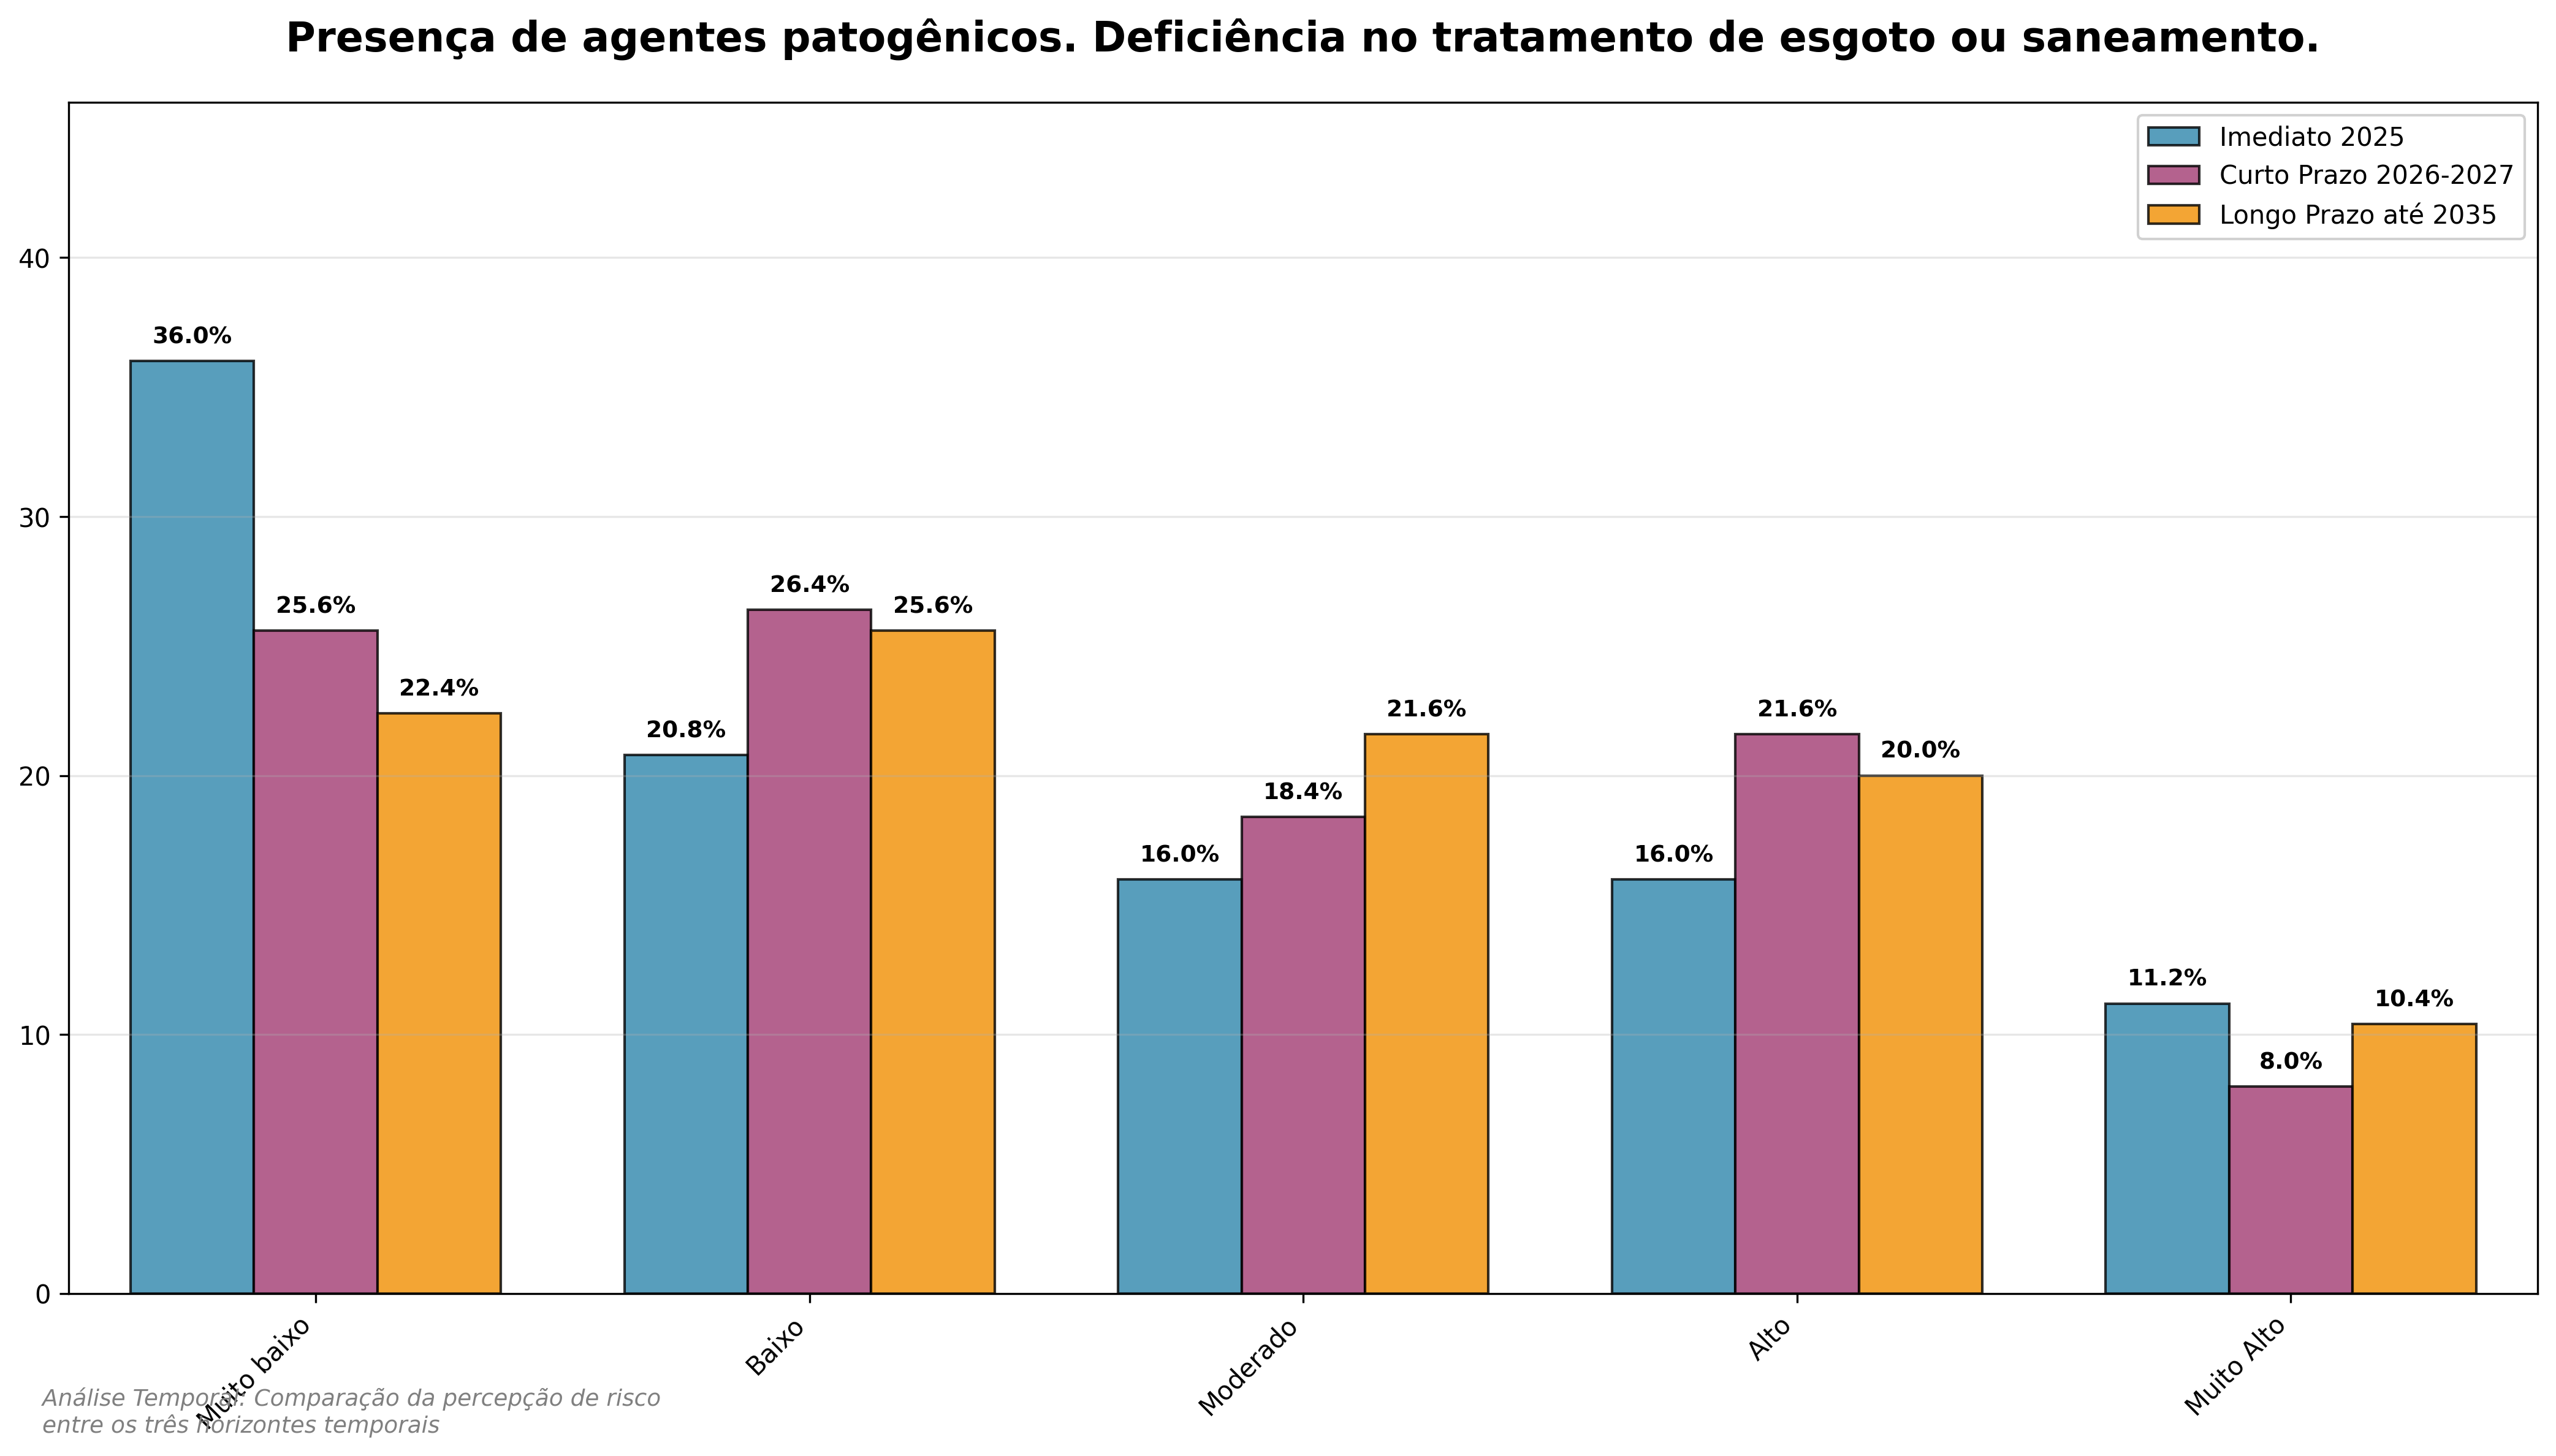
\includegraphics[keepaspectratio]{assets/ambientais/grafico_agrupado_2_9_temporal.png}}

\begin{tcolorbox}[enhanced jigsaw, titlerule=0mm, colback=white, title=\textcolor{quarto-callout-tip-color}{\faLightbulb}\hspace{0.5em}{Destaques}, opacityback=0, colbacktitle=quarto-callout-tip-color!10!white, leftrule=.75mm, left=2mm, colframe=quarto-callout-tip-color-frame, bottomrule=.15mm, bottomtitle=1mm, breakable, toprule=.15mm, toptitle=1mm, opacitybacktitle=0.6, arc=.35mm, coltitle=black, rightrule=.15mm]

\textbf{Evolução da Percepção de Risco:} os dados evidenciam uma
tendência de elevação gradual na percepção de risco associada à presença
de agentes patogênicos e à deficiência no tratamento de esgoto e nas
condições de saneamento básico, tanto no ambiente portuário quanto em
seu entorno.~

\textbf{Contexto Detalhado por Período:}

\textbf{Período Imediato (2025):} A percepção de risco é moderada, com
27\% dos respondentes classificando o risco como alto (4) ou muito alto
(5), e mediana igual a 2, indicando que, no curto prazo, o problema é
reconhecido, mas ainda restrito a situações pontuais ou controláveis.

\textbf{Curto Prazo (2026--2027):} Observa-se aumento gradual da
preocupação, com 30\% das respostas concentradas nos níveis alto ou
muito alto, mantendo mediana em 2, o que demonstra maior atenção à
relação entre saneamento, saúde pública e segurança ocupacional.

\textbf{Longo Prazo (até 2035):} a percepção de risco atinge seu ponto
mais elevado, com 30\% das respostas nos níveis 4--5 e mediana de 3,
refletindo reconhecimento crescente dos impactos sanitários e
reputacionais decorrentes da má gestão de efluentes e resíduos urbanos
próximos às áreas portuárias.

\textbf{Implicações Estratégicas}: a presença de agentes patogênicos,
associada à deficiência no tratamento de esgoto e nas condições de
saneamento, pode gerar riscos sanitários significativos para
trabalhadores portuários e comunidades do entorno. Essas condições podem
resultar em restrições de acesso a áreas operacionais, afastamento de
pessoal por motivos de saúde, e sanções ou autuações por órgãos de
vigilância sanitária, comprometendo tanto a saúde ocupacional quanto a
imagem institucional do complexo portuário. Para mitigar esses riscos, é
essencial adotar medidas como: ampliação da cobertura de saneamento e
drenagem, instalação de sistemas eficientes de tratamento de efluentes
sanitários e industriais, monitoramento microbiológico periódico da
qualidade da água, e programas de prevenção e saúde ocupacional voltados
à proteção dos trabalhadores expostos. Essas ações fortalecem a
resiliência sanitária e a governança ambiental do porto, contribuindo
para a sustentabilidade e a confiança institucional a longo prazo.

\end{tcolorbox}

\subsection{Introdução de espécies exóticas, organismos aquáticos
nocivos e agentes
patogênicos}\label{introduuxe7uxe3o-de-espuxe9cies-exuxf3ticas-organismos-aquuxe1ticos-nocivos-e-agentes-patoguxeanicos}

O gr?fico a seguir apresenta a evolu??o temporal do risco Introdução de
espécies exóticas, organismos aquáticos nocivos e agentes patogênicos.
\pandocbounded{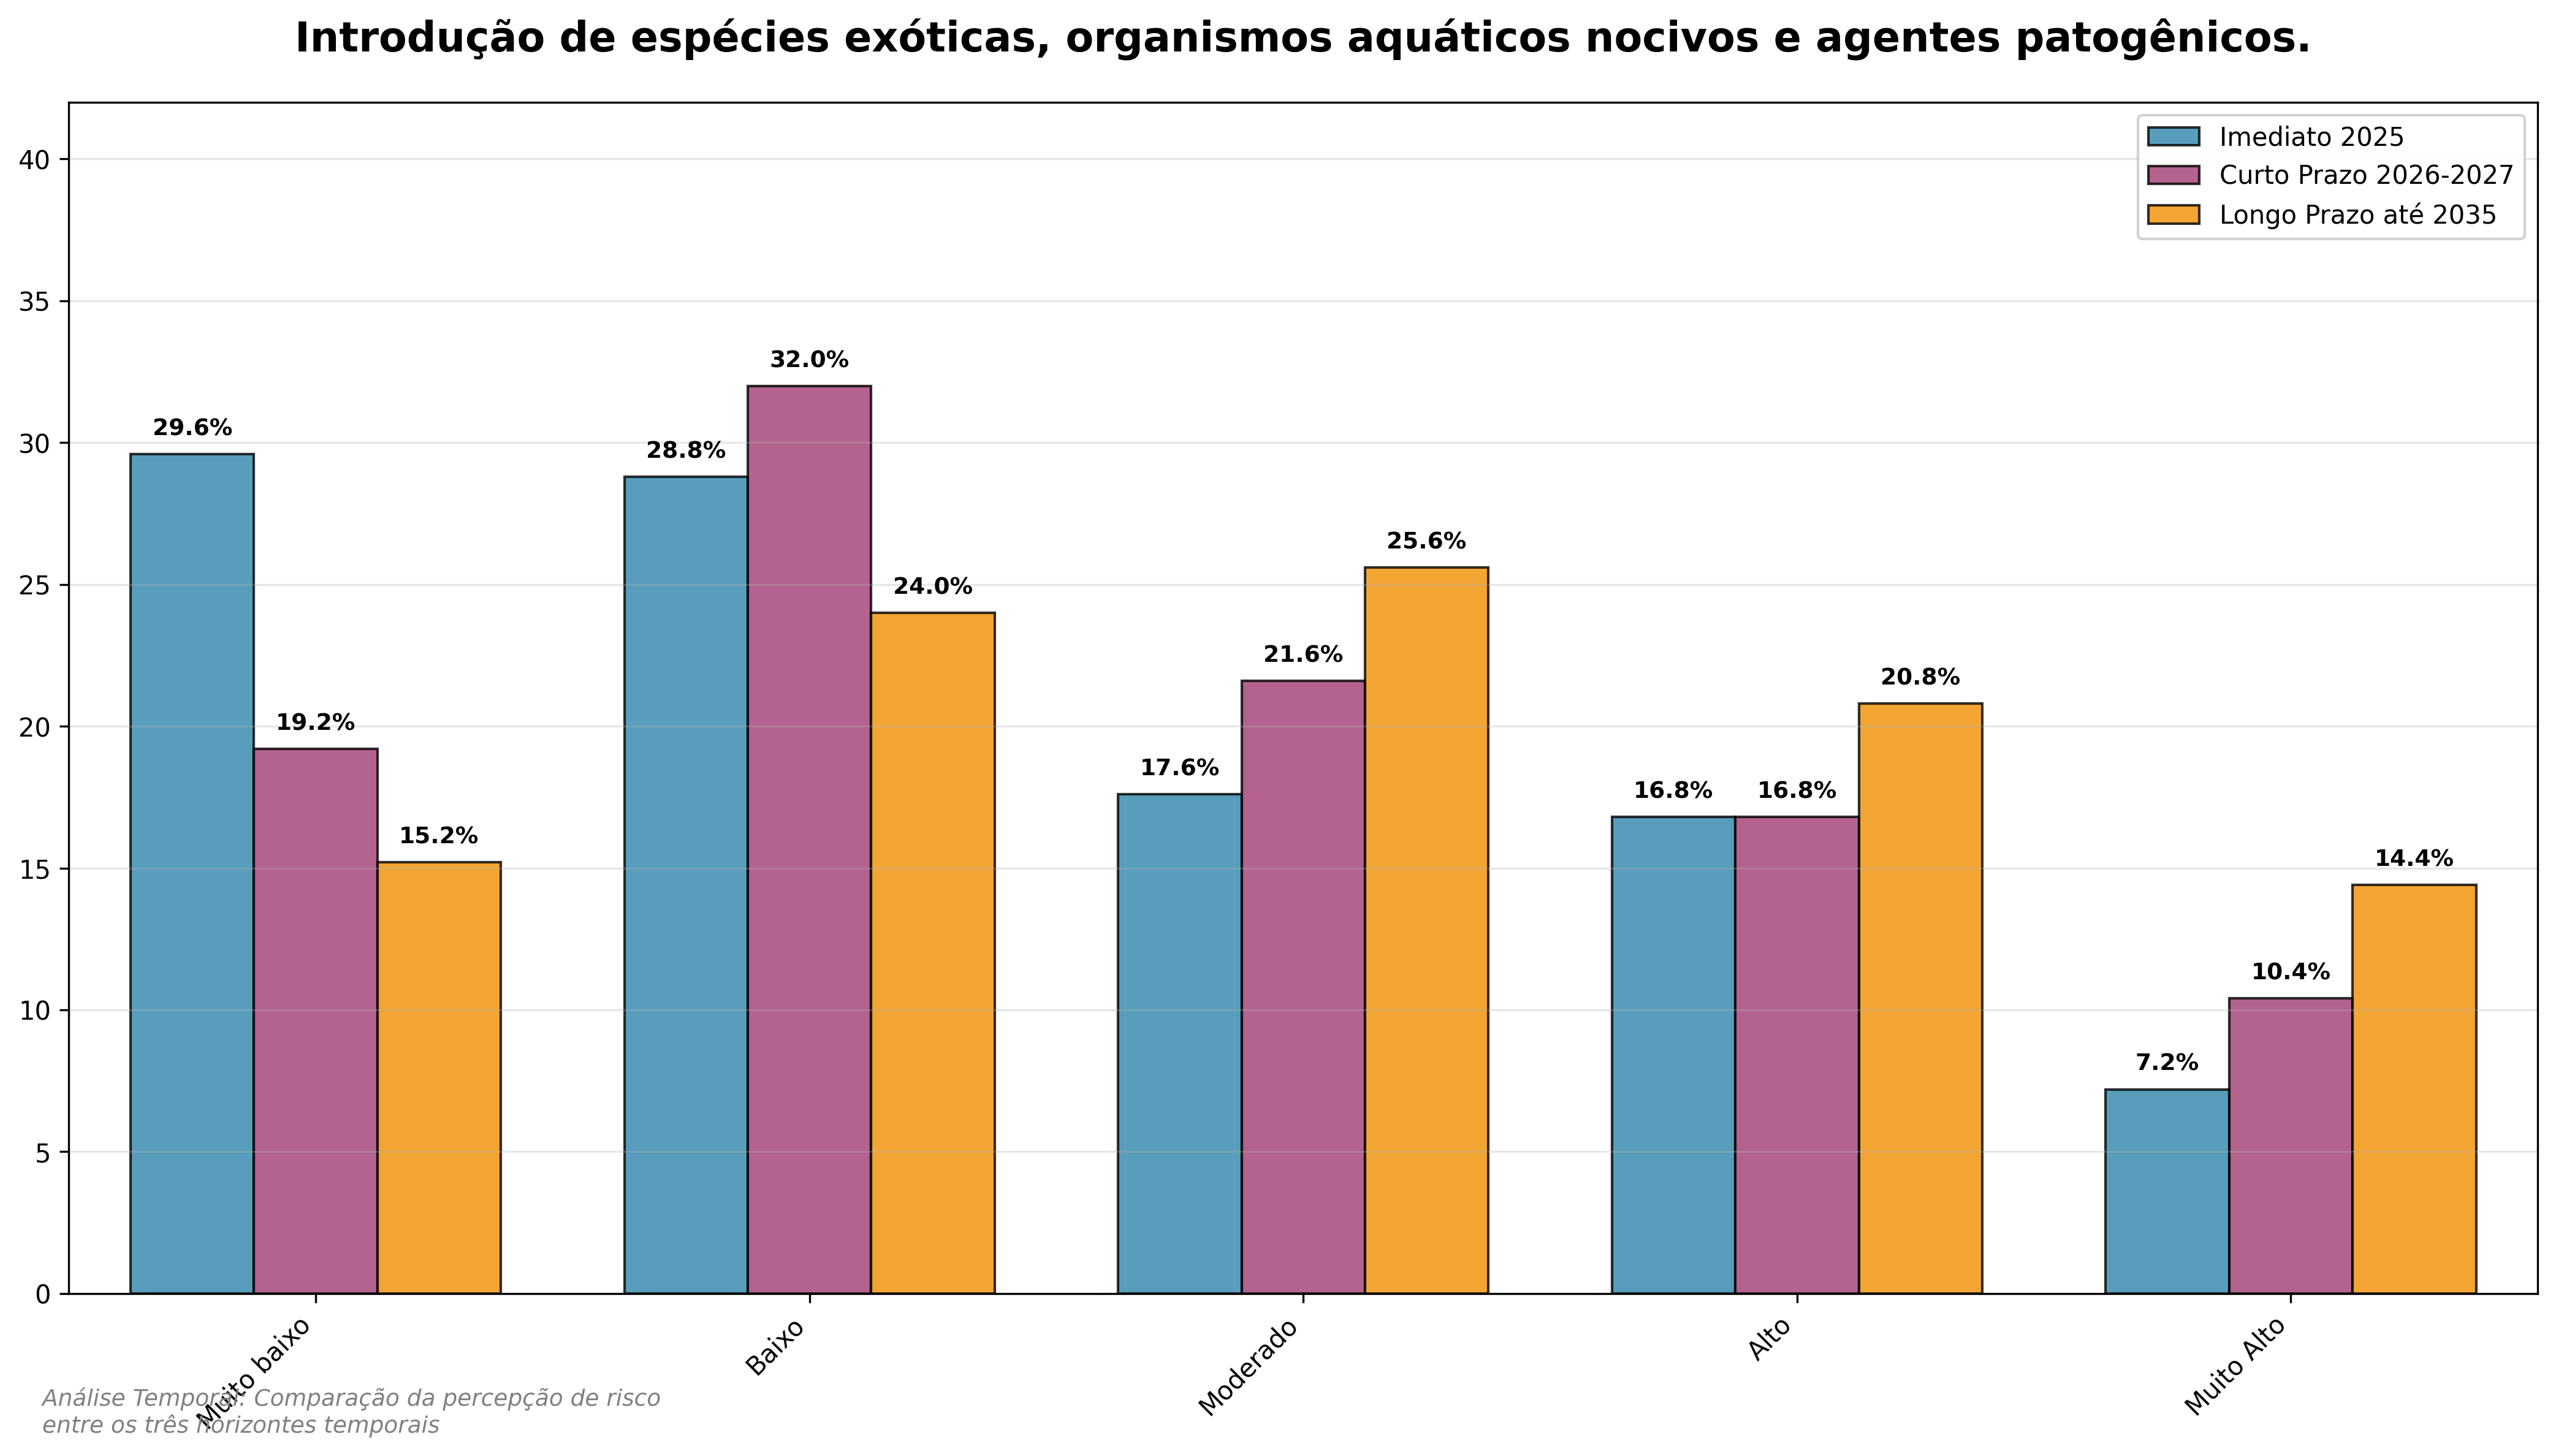
\includegraphics[keepaspectratio]{assets/ambientais/grafico_agrupado_2_10_temporal.png}}

\begin{tcolorbox}[enhanced jigsaw, titlerule=0mm, colback=white, title=\textcolor{quarto-callout-tip-color}{\faLightbulb}\hspace{0.5em}{Destaques}, opacityback=0, colbacktitle=quarto-callout-tip-color!10!white, leftrule=.75mm, left=2mm, colframe=quarto-callout-tip-color-frame, bottomrule=.15mm, bottomtitle=1mm, breakable, toprule=.15mm, toptitle=1mm, opacitybacktitle=0.6, arc=.35mm, coltitle=black, rightrule=.15mm]

\textbf{Evolução da Percepção de Risco:} O gráfico demonstra uma
tendência crescente de percepção de risco associada à introdução de
espécies exóticas invasoras, organismos aquáticos nocivos e agentes
patogênicos, fenômeno frequentemente vinculado à descarga de água de
lastro. Essa evolução sugere maior reconhecimento dos riscos ambientais
e regulatórios para o setor portuário.~

\textbf{Contexto Detalhado por Período:}

\textbf{Período Imediato (2025):} A percepção de risco é moderada, com
24\% das respostas classificando o risco como alto (4) ou muito alto
(5), e mediana igual a 2, indicando que, no horizonte mais próximo, os
impactos são percebidos como pontuais ou de baixa probabilidade.

\textbf{Curto Prazo (2026--2027):} Observa-se elevação gradual da
preocupação, com 27\% dos respondentes avaliando o risco como alto ou
muito alto, mantendo mediana em 2, refletindo maior atenção às
exigências regulatórias internacionais e à gestão de águas de lastro.

\textbf{Longo Prazo (até 2035):} A percepção de risco se intensifica
expressivamente, alcançando 35\% das respostas nos níveis alto (4) e
muito alto (5), e mediana igual a 3, evidenciando reconhecimento de que
a proliferação de espécies invasoras representa ameaça crescente à
biodiversidade marinha e às atividades portuárias.

\textbf{Implicações Estratégica:} A introdução de espécies exóticas
invasoras, organismos aquáticos nocivos e agentes patogênicos, seja por
descarga de água de lastro ou outro tipo de descarte pode causar
desequilíbrios ecológicos graves, com competição entre espécies nativas
e invasoras, alteração de habitats e danos irreversíveis à
biodiversidade local. Essas ocorrências podem demandar ações corretivas
onerosas e restrições adicionais de atracação e manuseio de embarcações,
impactando diretamente a conformidade ambiental e a reputação
institucional do porto. Entre as medidas preventivas prioritárias
destacam-se: monitoramento e registro contínuo das operações de lastro,
adoção de tecnologias de tratamento de água de lastro a bordo e~
capacitação das equipes para resposta rápida a incidentes ambientais.
Essas ações são fundamentais para assegurar a conformidade com normas
internacionais, preservar os ecossistemas costeiros e fortalecer a
governança ambiental do complexo portuário.

\end{tcolorbox}

\subsection{Poluição atmosférica}\label{poluiuxe7uxe3o-atmosfuxe9rica}

O gr?fico a seguir apresenta a evolu??o temporal do risco Poluição
atmosférica.
\pandocbounded{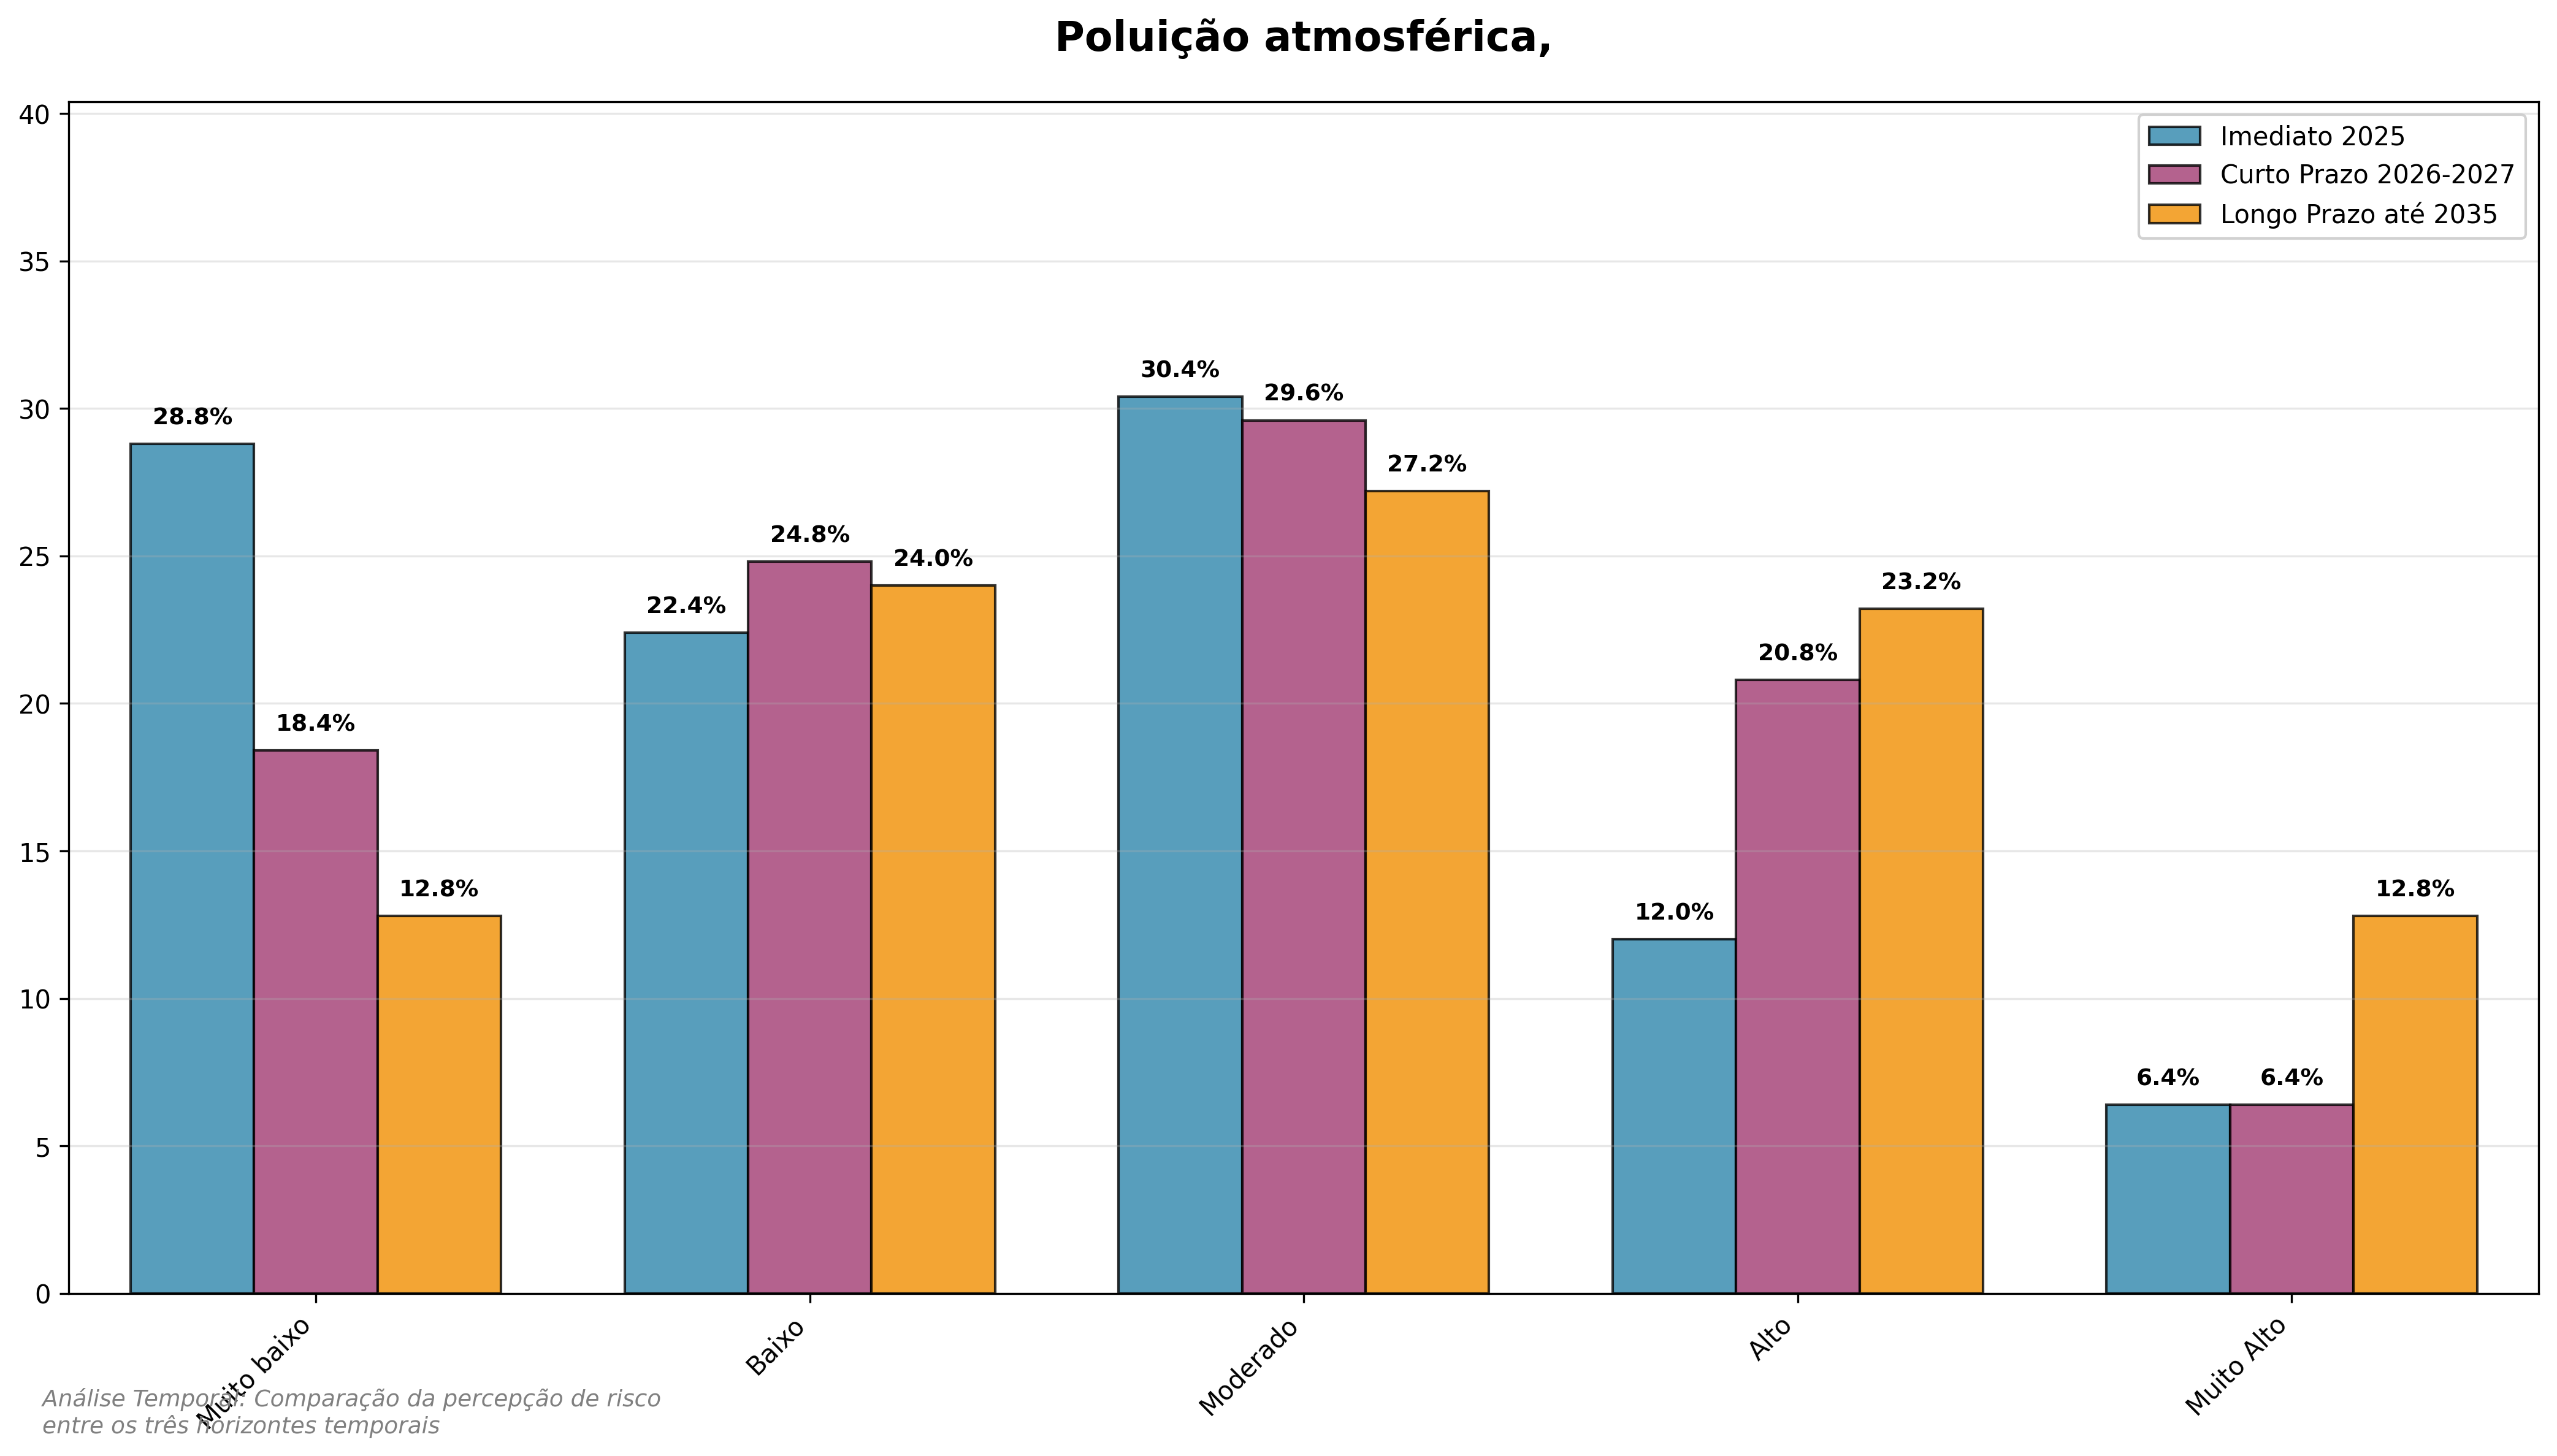
\includegraphics[keepaspectratio]{assets/ambientais/grafico_agrupado_2_11_temporal.png}}

\begin{tcolorbox}[enhanced jigsaw, titlerule=0mm, colback=white, title=\textcolor{quarto-callout-tip-color}{\faLightbulb}\hspace{0.5em}{Destaques}, opacityback=0, colbacktitle=quarto-callout-tip-color!10!white, leftrule=.75mm, left=2mm, colframe=quarto-callout-tip-color-frame, bottomrule=.15mm, bottomtitle=1mm, breakable, toprule=.15mm, toptitle=1mm, opacitybacktitle=0.6, arc=.35mm, coltitle=black, rightrule=.15mm]

\textbf{Evolução da Percepção de Risco:} O gráfico revela uma tendência
de aumento gradual na percepção de risco associada à poluição
atmosférica gerada pelas atividades portuárias e industriais,
especialmente com o avanço do horizonte temporal. A preocupação
crescente reflete o reconhecimento dos impactos das emissões de gases e
material particulado sobre a saúde pública, a regulação ambiental e as
metas de descarbonização do setor. Esse comportamento reflete a previsão
de maior rigor regulatório e pressão social sobre os portos para adoção
de tecnologias limpas e práticas sustentáveis, especialmente diante da
ampliação de políticas de neutralidade de carbono e das metas da IMO
para redução das emissões de GEE no transporte marítimo.

\textbf{Contexto Detalhado por Período:}

\textbf{Período Imediato (2025):} A percepção de risco é relativamente
baixa, com 18\% das respostas classificando o risco como alto (4) ou
muito alto (5) e mediana igual a 2, sugerindo que, no curto horizonte, o
problema é percebido como localizado ou sob controle operacional.

\textbf{Curto Prazo (2026--2027):} Há aumento considerável da
preocupação, com 27\% dos respondentes avaliando o risco como alto ou
muito alto, e mediana de 3, indicando maior consciência sobre a
contribuição das operações portuárias para as emissões atmosféricas e
seus reflexos sobre a qualidade do ar.

\textbf{Longo Prazo (até 2035):} A percepção de risco se intensifica
expressivamente, alcançando 36\% das respostas nos níveis 4-5, com
mediana mantida em 3, demonstrando preocupação crescente com o
cumprimento de normas ambientais mais rígidas e com o impacto cumulativo
das emissões sobre as comunidades portuárias.

\hfill\break
\textbf{Implicações Estratégicas:}~ A poluição atmosférica gerada por
embarcações atracadas, veículos, equipamentos portuários e atividades
industriais associadas pode levar ao aumento das concentrações de
material particulado e gases poluentes (como NOx, SOx e CO₂) na área de
influência do porto. Essas condições podem resultar em agravamento de
problemas respiratórios nas populações expostas, elevação da pressão
regulatória e exigência de mitigação de emissões, além de impactar
negativamente a aceitação social do empreendimento. Entre as principais
medidas de mitigação destacam-se: instalação de sistemas de fornecimento
de energia em terra, substituição progressiva de equipamentos e veículos
por versões eletrificadas ou híbridas, uso de combustíveis de baixo
carbono e filtros antipoluição, e monitoramento contínuo da qualidade do
ar nas zonas portuárias e urbanas adjacentes. A adoção dessas práticas é
essencial para garantir a conformidade com as metas de descarbonização,
fortalecer a reputação institucional e contribuir para a
sustentabilidade e competitividade do porto em longo prazo.

\textbf{Evolução da Percepção de Risco:} O gráfico revela uma tendência
de aumento gradual na percepção de risco associada à poluição
atmosférica gerada pelas atividades portuárias e industriais,
especialmente com o avanço do horizonte temporal. A preocupação
crescente reflete o reconhecimento dos impactos das emissões de gases e
material particulado sobre a saúde pública, a regulação ambiental e as
metas de descarbonização do setor. Esse comportamento reflete a previsão
de maior rigor regulatório e pressão social sobre os portos para adoção
de tecnologias limpas e práticas sustentáveis, especialmente diante da
ampliação de políticas de neutralidade de carbono e das metas da IMO
para redução das emissões de GEE no transporte marítimo.

\textbf{Contexto Detalhado por Período:}

\textbf{Período Imediato (2025):} A percepção de risco é relativamente
baixa, com 18\% das respostas classificando o risco como alto (4) ou
muito alto (5) e mediana igual a 2, sugerindo que, no curto horizonte, o
problema é percebido como localizado ou sob controle operacional.

\textbf{Curto Prazo (2026--2027):} Há aumento considerável da
preocupação, com 27\% dos respondentes avaliando o risco como alto ou
muito alto, e mediana de 3, indicando maior consciência sobre a
contribuição das operações portuárias para as emissões atmosféricas e
seus reflexos sobre a qualidade do ar.

\textbf{Longo Prazo (até 2035):} A percepção de risco se intensifica
expressivamente, alcançando 36\% das respostas nos níveis 4-5, com
mediana mantida em 3, demonstrando preocupação crescente com o
cumprimento de normas ambientais mais rígidas e com o impacto cumulativo
das emissões sobre as comunidades portuárias.

\hfill\break
\textbf{Implicações Estratégicas:}~ A poluição atmosférica gerada por
embarcações atracadas, veículos, equipamentos portuários e atividades
industriais associadas pode levar ao aumento das concentrações de
material particulado e gases poluentes (como NOx, SOx e CO₂) na área de
influência do porto. Essas condições podem resultar em agravamento de
problemas respiratórios nas populações expostas, elevação da pressão
regulatória e exigência de mitigação de emissões, além de impactar
negativamente a aceitação social do empreendimento. Entre as principais
medidas de mitigação destacam-se: instalação de sistemas de fornecimento
de energia em terra, substituição progressiva de equipamentos e veículos
por versões eletrificadas ou híbridas, uso de combustíveis de baixo
carbono e filtros antipoluição, e monitoramento contínuo da qualidade do
ar nas zonas portuárias e urbanas adjacentes. A adoção dessas práticas é
essencial para garantir a conformidade com as metas de descarbonização,
fortalecer a reputação institucional e contribuir para a
sustentabilidade e competitividade do porto em longo prazo.

\end{tcolorbox}

\subsection{Ruídos e vibrações}\label{ruuxeddos-e-vibrauxe7uxf5es}

O gr?fico a seguir apresenta a evolu??o temporal do risco Ruídos e
vibrações.
\pandocbounded{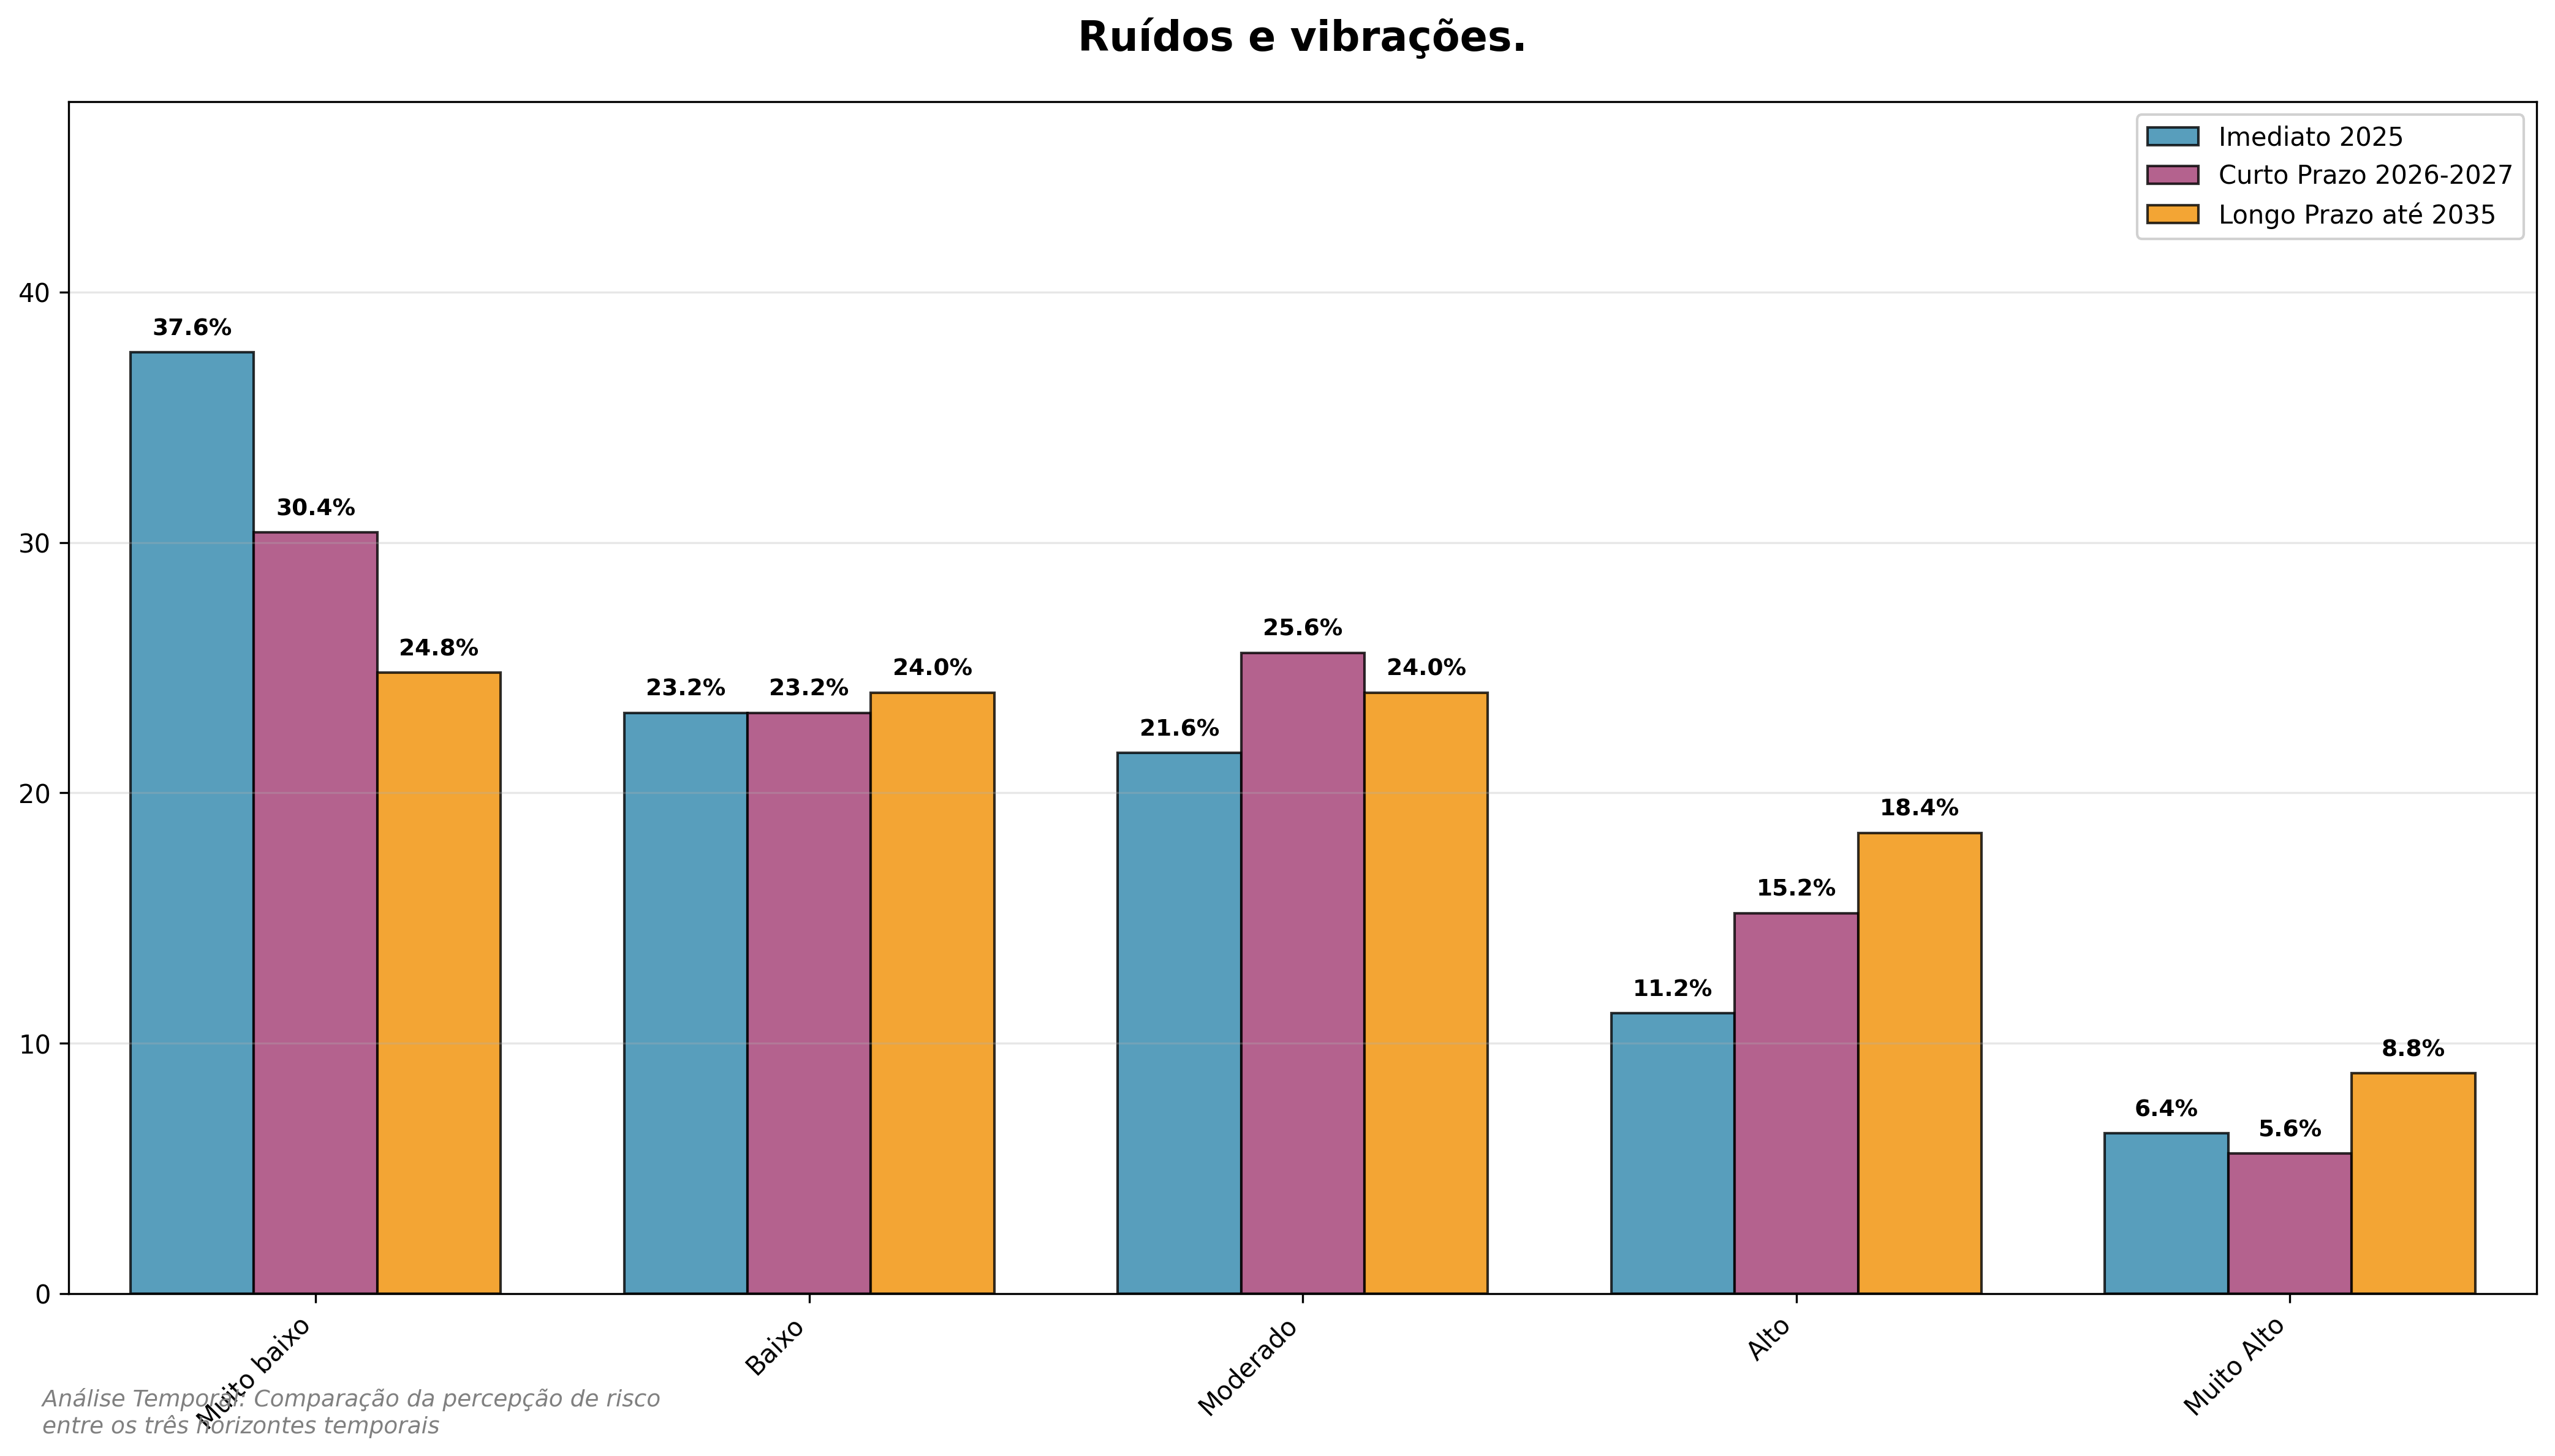
\includegraphics[keepaspectratio]{assets/ambientais/grafico_agrupado_2_12_temporal.png}}

\begin{tcolorbox}[enhanced jigsaw, titlerule=0mm, colback=white, title=\textcolor{quarto-callout-tip-color}{\faLightbulb}\hspace{0.5em}{Destaques}, opacityback=0, colbacktitle=quarto-callout-tip-color!10!white, leftrule=.75mm, left=2mm, colframe=quarto-callout-tip-color-frame, bottomrule=.15mm, bottomtitle=1mm, breakable, toprule=.15mm, toptitle=1mm, opacitybacktitle=0.6, arc=.35mm, coltitle=black, rightrule=.15mm]

\textbf{Evolução da Percepção de Risco:} O gráfico indica uma tendência
de aumento gradual na percepção de risco relacionada a ruídos e
vibrações provenientes das operações portuárias (movimentação de cargas,
guindastes, equipamentos de pátio e tráfego pesado), indicando
vulnerabilidade crescente do relacionamento porto-cidade a esse tema.

\textbf{Contexto Detalhado por Período:}

\textbf{Imediato (2025):} 18\% dos respondentes classificam o risco como
alto (4) ou muito alto (5) e mediana igual a 2. Predomina a leitura de
risco baixo a moderado no curtíssimo prazo.

\textbf{Curto Prazo (2026--2027):} 21\% em níveis 4-5 e mediana igual a
2. Sinaliza elevação discreta da preocupação, com maior atenção a
incômodos crônicos e reclamações da vizinhança.

\textbf{Longo Prazo (até 2035):} 27\% em 4-5 e mediana igual a 3. A
percepção se intensifica, refletindo expectativa de maior pressão social
e regulatória e de expansão operacional que amplia fontes de ruído e
vibração.

\textbf{Implicações Estratégicas:} Os ruídos e vibrações associados à
movimentação de cargas, operação de guindastes, equipamentos de pátio e
tráfego de veículos pesados podem gerar incômodos crônicos e efeitos
adversos à saúde e ao bem-estar de comunidades vizinhas e trabalhadores.
Tais condições podem levar a restrições de horários de operação,
exigência de barreiras acústicas, adequações de layout e até ações
judiciais de moradores, comprometendo o relacionamento porto-cidade e a
flexibilidade operacional do terminal. Dente as medidas recomendadas
destacam-se: planos de gestão de ruído com metas e monitoramento
contínuo e painéis públicos e zonas tampão, barreiras acústicas e
revisão de rotas internas para reduzir exposição.

\end{tcolorbox}

\subsection{Gerenciamento inadequado dos resíduos
sólidos}\label{gerenciamento-inadequado-dos-resuxedduos-suxf3lidos}

O gr?fico a seguir apresenta a evolu??o temporal do risco Gerenciamento
inadequado dos resíduos sólidos.
\pandocbounded{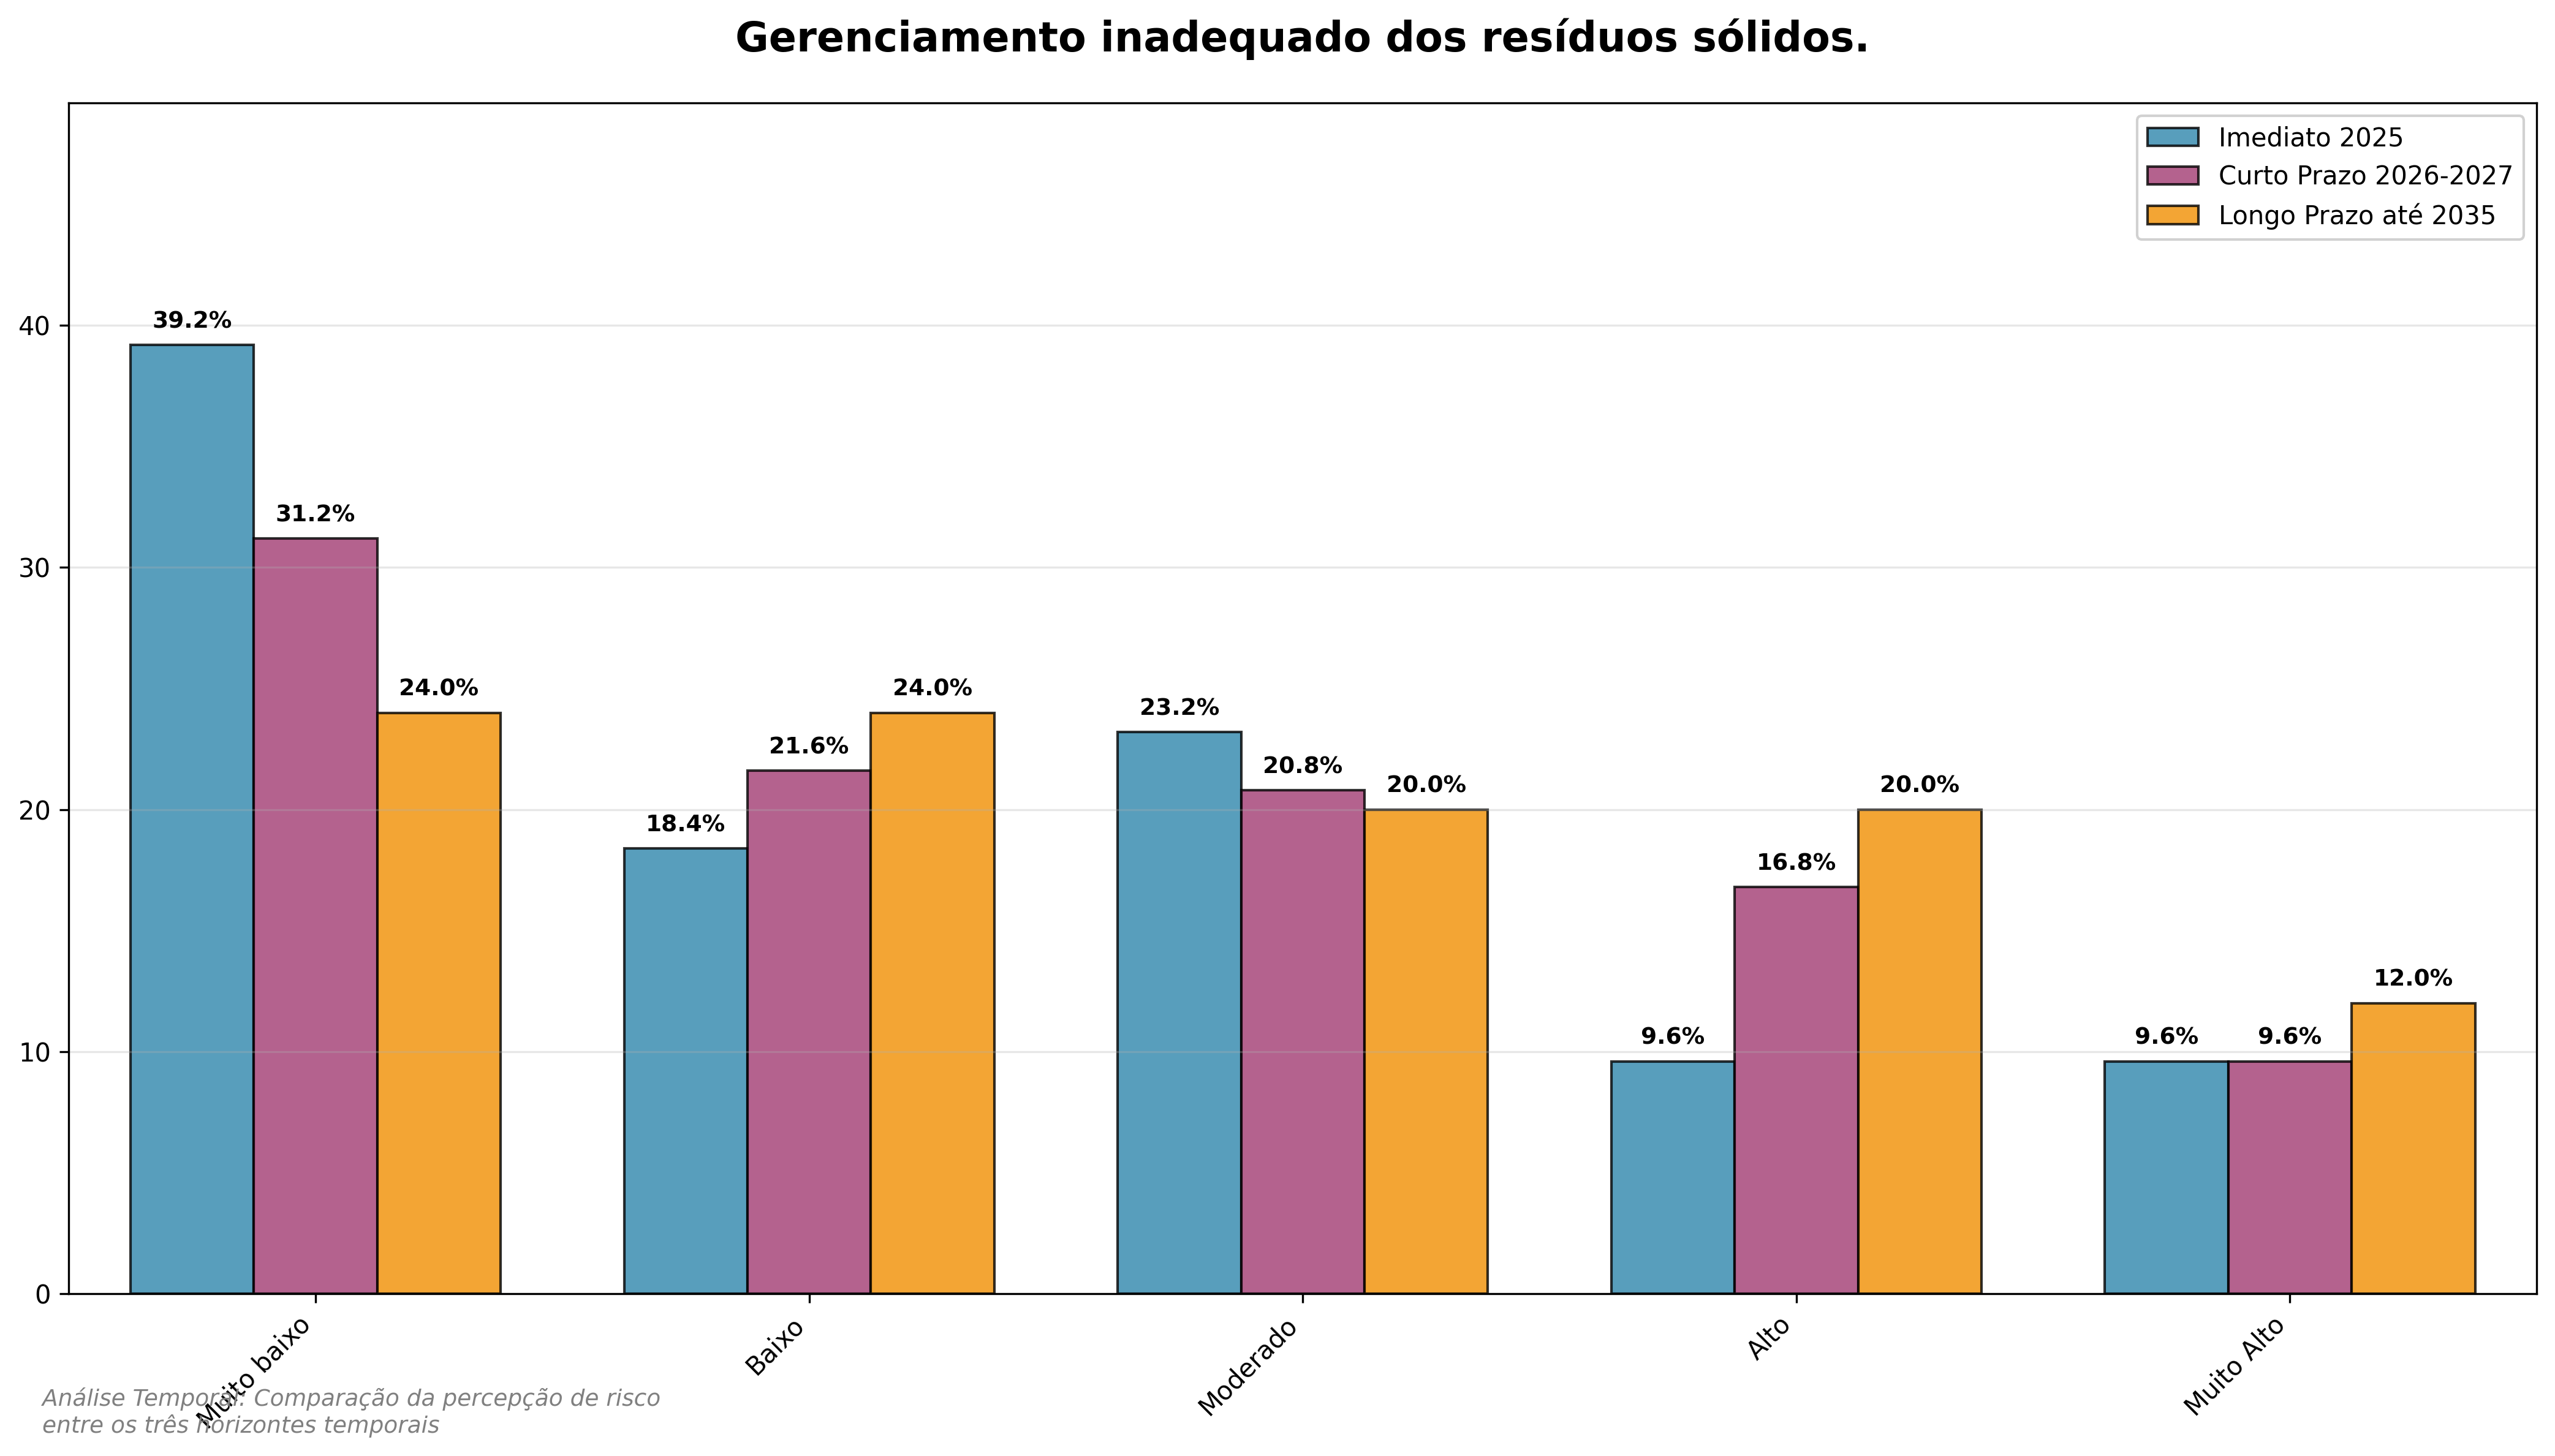
\includegraphics[keepaspectratio]{assets/ambientais/grafico_agrupado_2_13_temporal.png}}

\begin{tcolorbox}[enhanced jigsaw, titlerule=0mm, colback=white, title=\textcolor{quarto-callout-tip-color}{\faLightbulb}\hspace{0.5em}{Destaques}, opacityback=0, colbacktitle=quarto-callout-tip-color!10!white, leftrule=.75mm, left=2mm, colframe=quarto-callout-tip-color-frame, bottomrule=.15mm, bottomtitle=1mm, breakable, toprule=.15mm, toptitle=1mm, opacitybacktitle=0.6, arc=.35mm, coltitle=black, rightrule=.15mm]

\textbf{Evolução da Percepção de Risco:} O gráfico indica uma tendência
de aumento gradual na percepção de risco relacionada ao gerenciamento
inadequado dos resíduos sólidos.

\textbf{Contexto Detalhado por Período:}

\textbf{Imediato (2025):} 19\% dos respondentes classificam o risco como
alto (4) ou muito alto (5) e mediana igual a 2. Predomina a percepção de
risco baixo a moderado no horizonte mais próximo.

\textbf{Curto Prazo (2026--2027):} 26\% em níveis 4-5 e mediana igual a
2. Observa-se elevação da preocupação, com maior atenção à conformidade
ambiental e ao aumento do volume de resíduos.

\textbf{Longo Prazo (até 2035):} 32\% em 4-5 e mediana igual a 3. A
percepção se intensifica, refletindo expectativa de maior pressão
regulatória e de necessidade de investimentos em infraestrutura e
monitoramento.

\textbf{Implicações Estratégicas:} O gerenciamento inadequado de
resíduos sólidos pode resultar em descarte irregular, acúmulo em áreas
ambientalmente sensíveis e contaminação do solo e dos recursos hídricos.
Essas condições podem gerar autuações ambientais, interdição de áreas
operacionais e comprometimento da credibilidade institucional,
impactando negativamente a governança ambiental e o cumprimento das
metas de sustentabilidade do complexo portuário. Dentre as medidas
recomendadas destacam-se: Plano de Gerenciamento de Resíduos Sólidos
(PGRS) revisado, com metas e indicadores; segregação na origem, rotas
internas otimizadas e rastreabilidade por TI; infraestrutura dedicada e
impermeabilizada para armazenamento temporário; contratos e licenças
atualizados de transportadores e destinadores; programas de capacitação
contínua e transparência dos resultados por meio de relatórios públicos.
Essas ações fortalecem a conformidade legal, reduzem passivos e
consolidam a sustentabilidade operacional dos portos a longo prazo.

\end{tcolorbox}

\subsection{Desmatamento}\label{desmatamento}

O gr?fico a seguir apresenta a evolu??o temporal do risco Desmatamento.
\pandocbounded{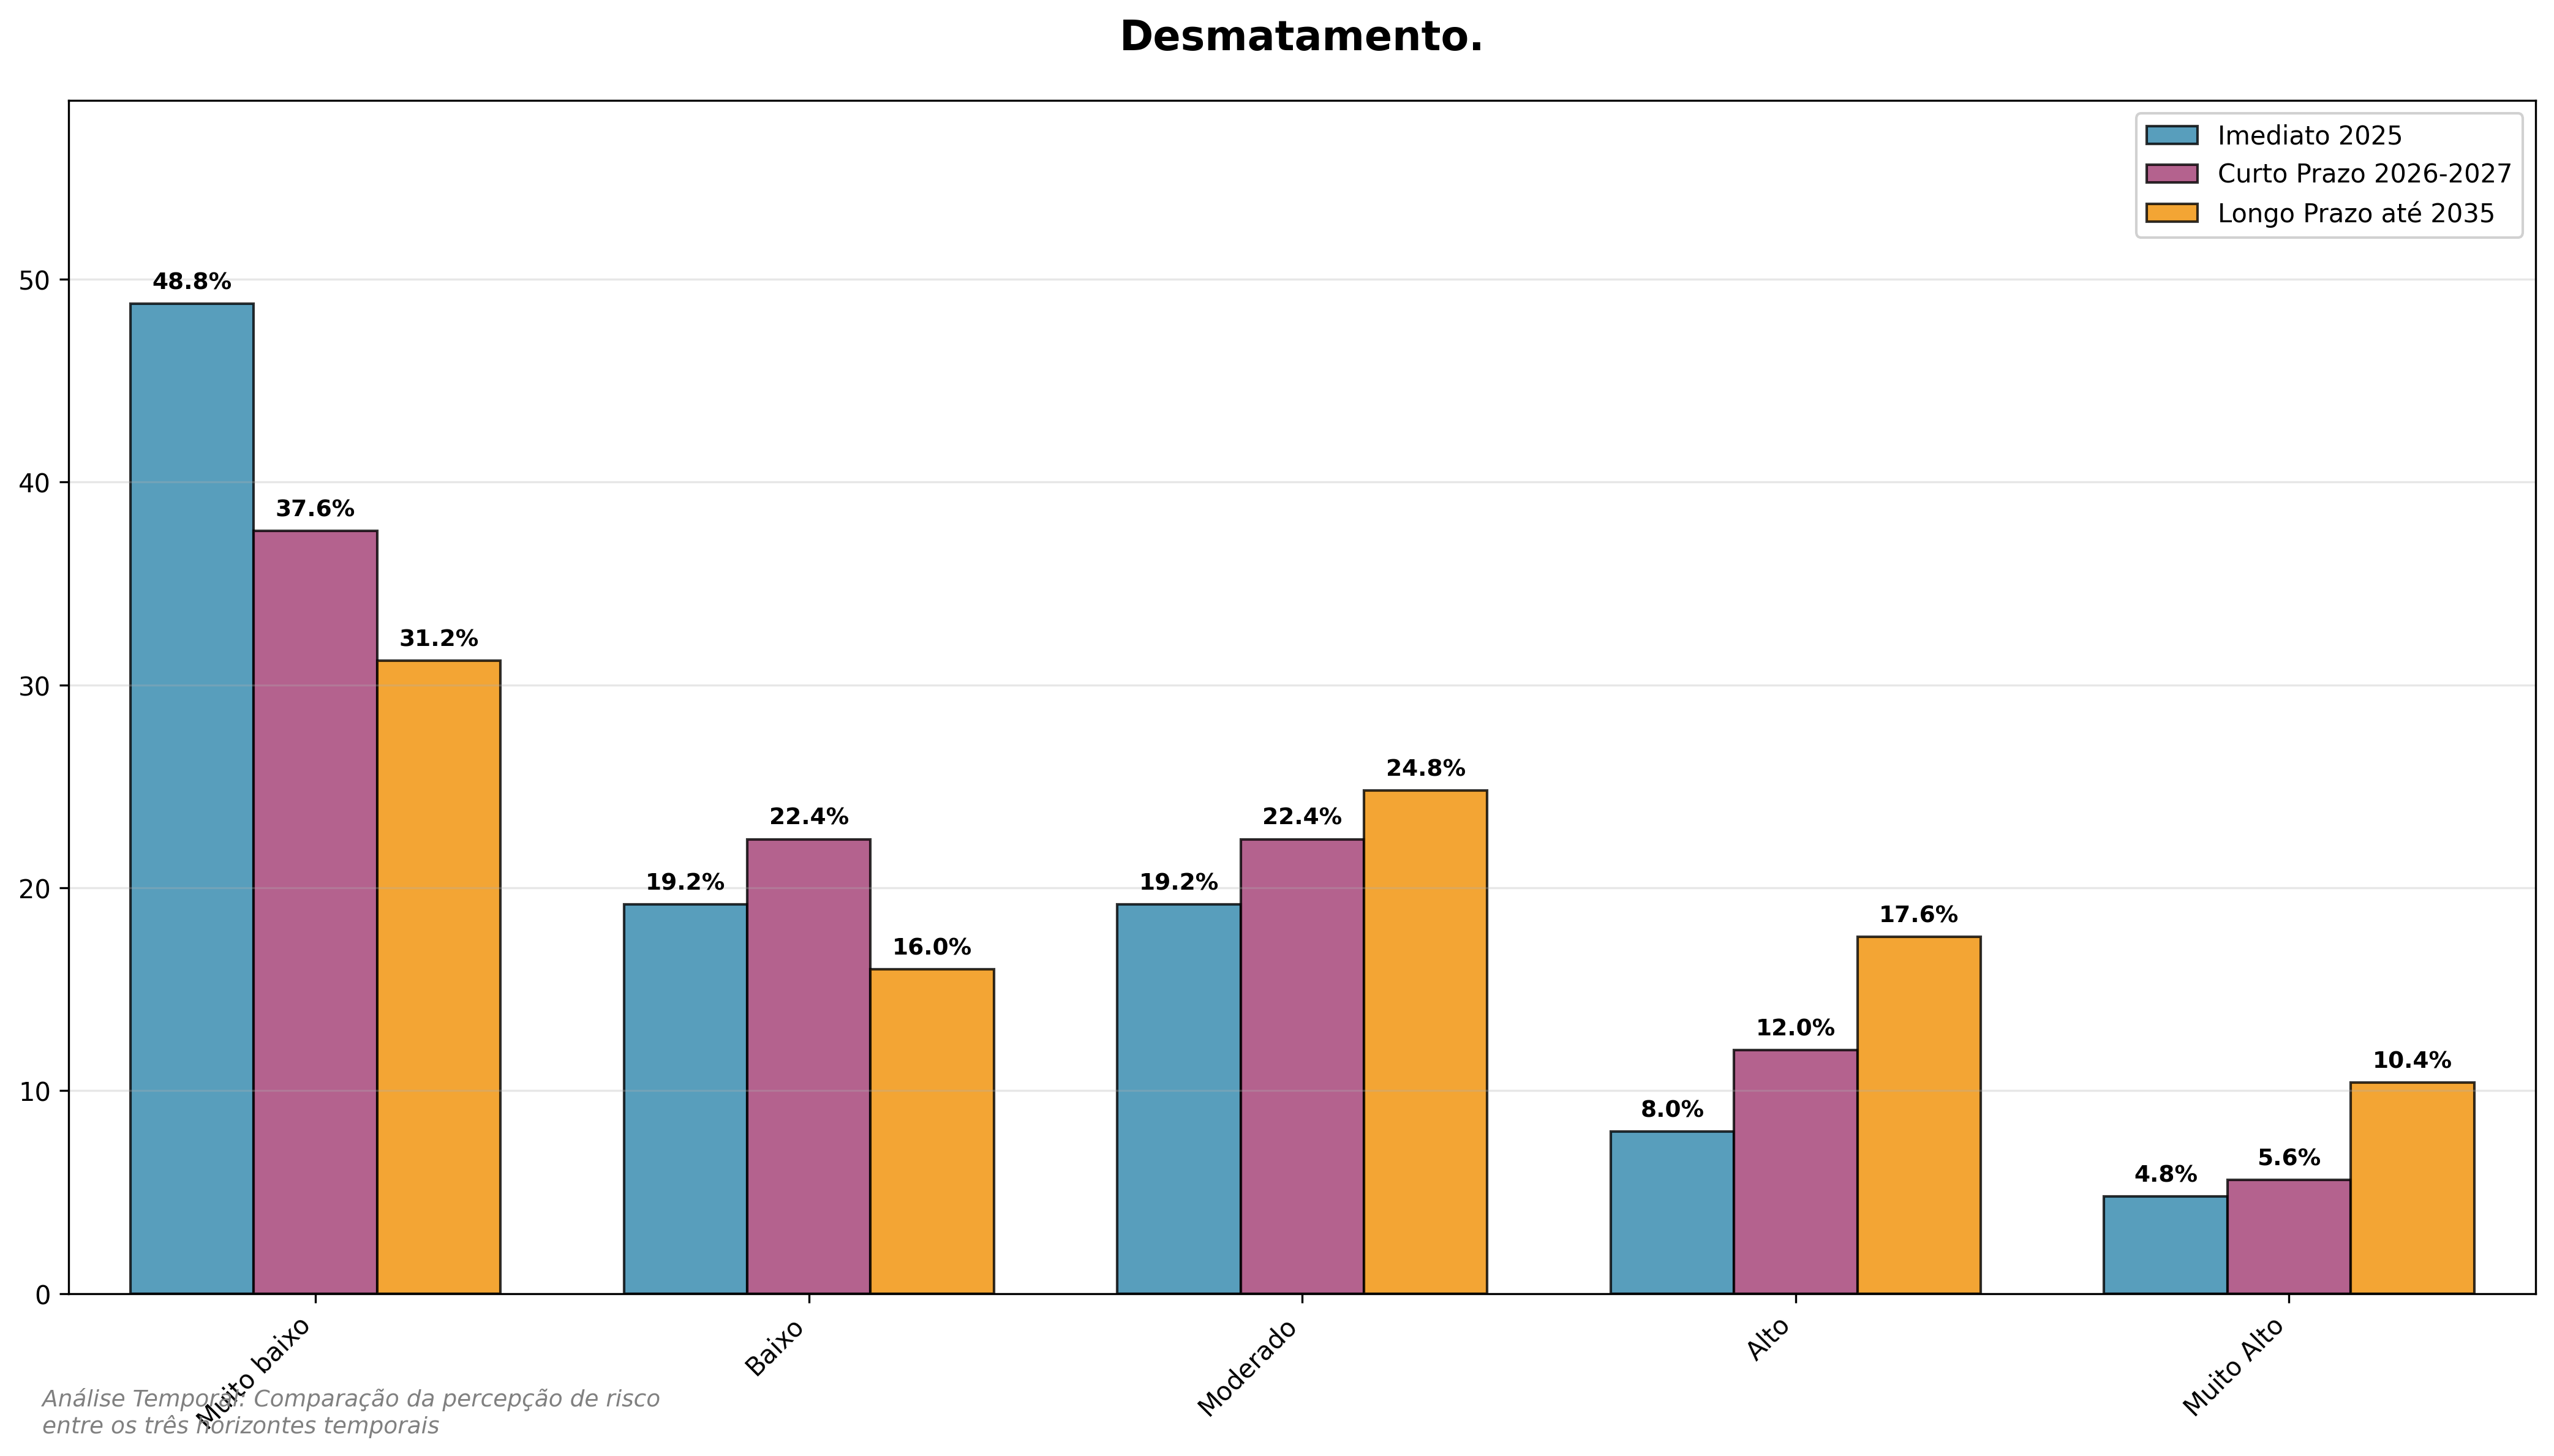
\includegraphics[keepaspectratio]{assets/ambientais/grafico_agrupado_2_14_temporal.png}}

\begin{tcolorbox}[enhanced jigsaw, titlerule=0mm, colback=white, title=\textcolor{quarto-callout-tip-color}{\faLightbulb}\hspace{0.5em}{Destaques}, opacityback=0, colbacktitle=quarto-callout-tip-color!10!white, leftrule=.75mm, left=2mm, colframe=quarto-callout-tip-color-frame, bottomrule=.15mm, bottomtitle=1mm, breakable, toprule=.15mm, toptitle=1mm, opacitybacktitle=0.6, arc=.35mm, coltitle=black, rightrule=.15mm]

\begin{longtable}[]{@{}
  >{\raggedright\arraybackslash}p{(\linewidth - 0\tabcolsep) * \real{1.0010}}@{}}
\toprule\noalign{}
\endhead
\bottomrule\noalign{}
\endlastfoot
\textbf{Evolução da Percepção de Risco:} Os dados indicam uma tendência
de aumento gradual da percepção de risco relacionada ao desmatamento,
especialmente em função da expansão portuária, abertura de acessos
logísticos e pressão por novas áreas industriais retroportuárias.

\textbf{Contexto Detalhado por Período:}

\textbf{Imediato (2025):} 13\% dos respondentes classificam o risco como
alto (4) ou muito alto (5) e mediana igual a 2. A percepção é
predominantemente baixa, sugerindo que o tema ainda é visto como um
risco indireto ou de ocorrência restrita. \textbar{}

\textbf{Curto Prazo (2026--2027):} 18\% em níveis 4-5 e mediana igual a
2. Observa-se elevação moderada da preocupação, refletindo maior
reconhecimento da influência das atividades portuárias sobre áreas de
vegetação nativa e ecossistemas adjacentes. \textbar{}

\textbf{Longo Prazo (até 2035):} 28\% em 4-5 e mediana igual a 3. A
percepção de risco se intensifica significativamente, demonstrando
expectativa de ampliação dos impactos cumulativos e das exigências
regulatórias e compensatórias relacionadas à supressão de cobertura
vegetal.

\textbf{Implicações Estratégicas:} O desmatamento associado à expansão
portuária, à abertura de acessos logísticos ou à criação de novas áreas
retroportuárias pode acarretar supressão de vegetação nativa e perda de
habitats ecologicamente sensíveis. Esses impactos podem gerar conflitos
socioambientais, judicialização dos processos de licenciamento e aumento
das exigências compensatórias, comprometendo a viabilidade econômica e a
reputação ambiental dos empreendimentos portuários. Dentre as medidas
recomendadas destacam-se: adoção de critérios de planejamento
territorial ambientalmente orientados; implementação de programas de
restauração florestal e compensação ecológica; integração de sistemas de
monitoramento por sensoriamento remoto; fortalecimento de estudos de
fauna e flora nos EIA/RIMA; e diálogo permanente com comunidades locais
e órgãos ambientais. Essas ações contribuem para minimizar os impactos
ambientais diretos e indiretos, assegurando conformidade legal e
legitimidade socioambiental aos projetos de expansão portuária. \\
\end{longtable}

\end{tcolorbox}

\subsection{Licenciamento ambiental}\label{licenciamento-ambiental}

O gr?fico a seguir apresenta a evolu??o temporal do risco Licenciamento
ambiental.
\pandocbounded{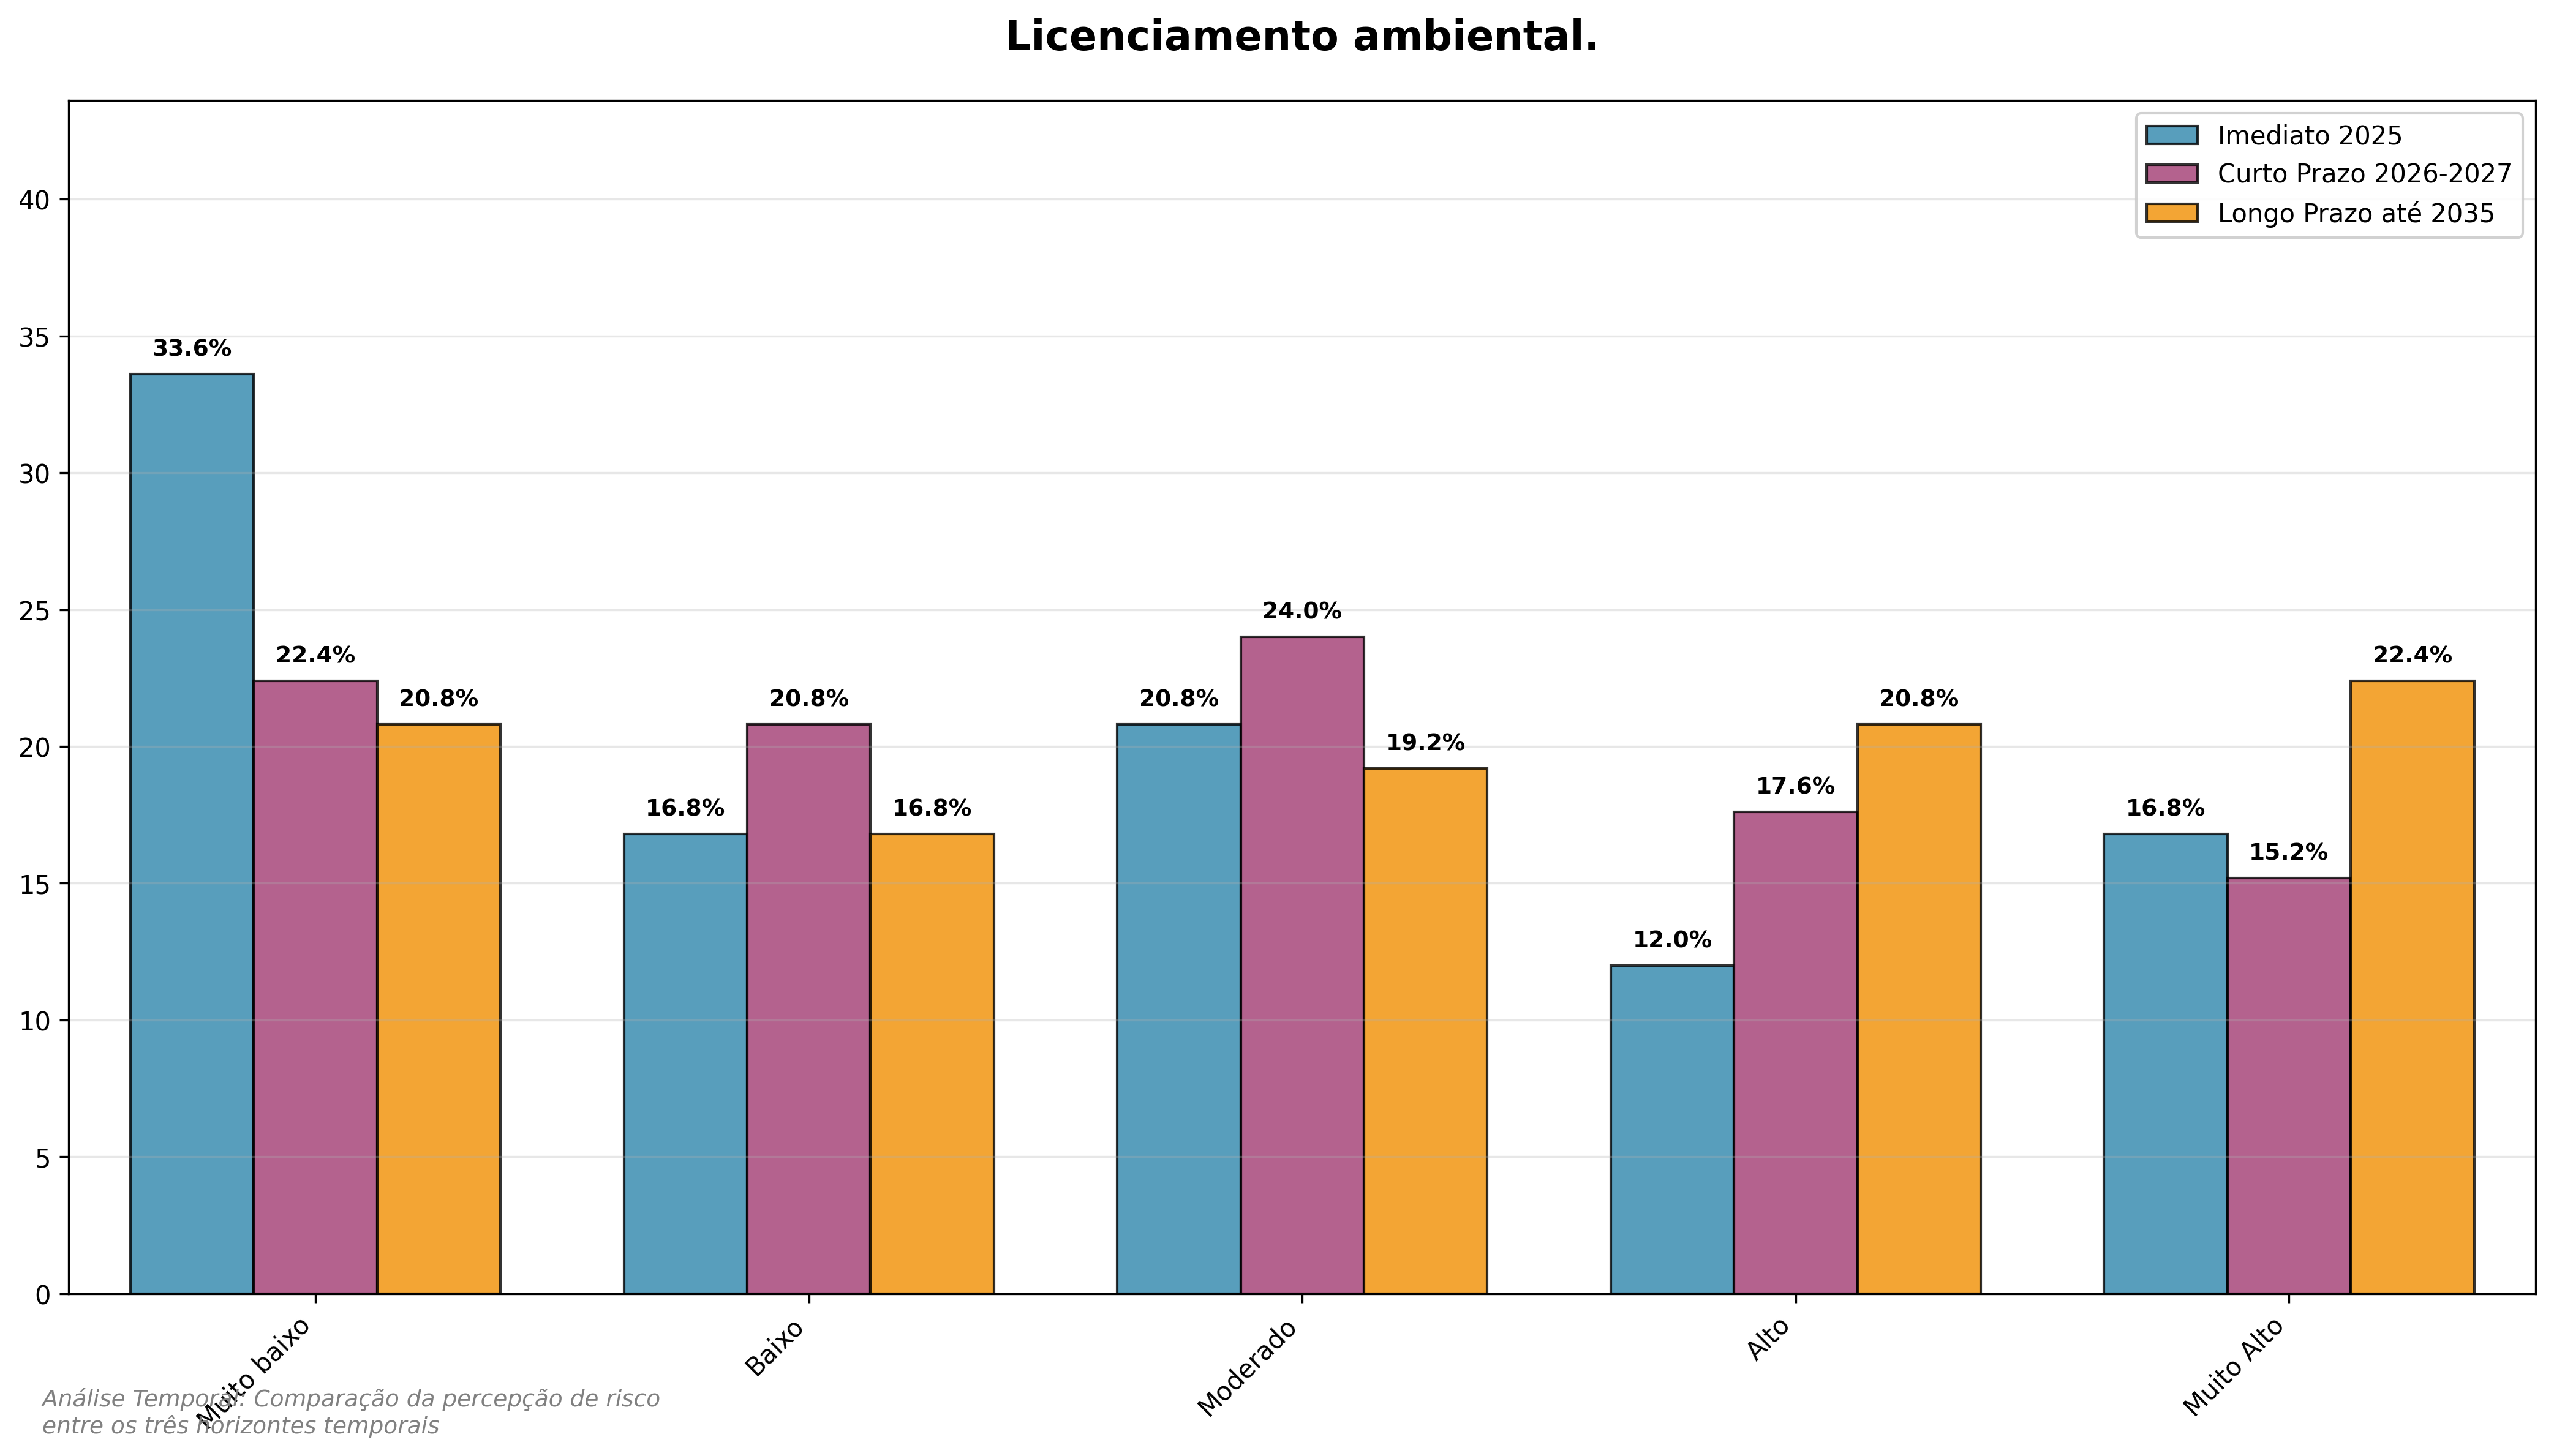
\includegraphics[keepaspectratio]{assets/ambientais/grafico_agrupado_2_15_temporal.png}}

\begin{tcolorbox}[enhanced jigsaw, titlerule=0mm, colback=white, title=\textcolor{quarto-callout-tip-color}{\faLightbulb}\hspace{0.5em}{Destaques}, opacityback=0, colbacktitle=quarto-callout-tip-color!10!white, leftrule=.75mm, left=2mm, colframe=quarto-callout-tip-color-frame, bottomrule=.15mm, bottomtitle=1mm, breakable, toprule=.15mm, toptitle=1mm, opacitybacktitle=0.6, arc=.35mm, coltitle=black, rightrule=.15mm]

\begin{longtable}[]{@{}
  >{\raggedright\arraybackslash}p{(\linewidth - 0\tabcolsep) * \real{1.0010}}@{}}
\toprule\noalign{}
\endhead
\bottomrule\noalign{}
\endlastfoot
\textbf{Evolução da Percepção de Risco:} O gráfico indica uma tendência
de aumento expressivo na percepção de risco associada ao licenciamento
ambiental, refletindo a crescente complexidade dos processos
regulatórios e o potencial impacto de atrasos, indeferimentos ou
exigências adicionais sobre a execução de projetos portuários.

\textbf{Contexto Detalhado por Período:}

\textbf{Imediato (2025):} 29\% dos respondentes classificam o risco como
alto (4) ou muito alto (5) e mediana igual a 2. Predomina a percepção de
risco moderado, com reconhecimento das dificuldades burocráticas já
existentes, mas sem grandes impactos operacionais imediatos. \textbar{}

\textbf{Curto Prazo (2026--2027):} 33\% em níveis 4-5 e mediana igual a
3. Observa-se aumento da preocupação, com destaque para a intensificação
das exigências ambientais e a ampliação dos prazos de análise nos órgãos
licenciadores. \textbar{}

\textbf{Longo Prazo (até 2035):} 43\% em 4-5 e mediana igual a 3. A
percepção de risco torna-se significativamente mais elevada, refletindo
expectativa de maior rigor regulatório, pressão social e
imprevisibilidade jurídica nos processos de licenciamento ambiental.
\textbar{}

\textbf{Implicações Estratégicas:} As fragilidades, atrasos ou não
conformidades nos processos de licenciamento ambiental podem resultar em
suspensão de obras, imposição de medidas adicionais de controle e
restrição de autorizações operacionais. Essas condições acarretam
aumento de prazos e custos, além de incertezas que afetam investimentos
estratégicos e a credibilidade institucional do porto. Dentre as medidas
recomendadas destacam-se: planejamento prévio de licenciamento integrado
às fases de projeto, fortalecimento das equipes técnicas de meio
ambiente, monitoramento contínuo das condicionantes e prazos, uso de
sistemas digitais de gestão de licenças, e interlocução proativa com os
órgãos ambientais. Também é essencial o engajamento transparente com
comunidades e partes interessadas, de modo a reduzir riscos de
judicialização e reforçar a previsibilidade regulatória. Essas ações
contribuem para mitigar atrasos, garantir a conformidade legal e
assegurar a sustentabilidade dos processos de expansão portuária. \\
\end{longtable}

\end{tcolorbox}

\subsection{Descarbonização do transporte
marítimo}\label{descarbonizauxe7uxe3o-do-transporte-maruxedtimo}

O gr?fico a seguir apresenta a evolu??o temporal do risco
Descarbonização do transporte marítimo.
\pandocbounded{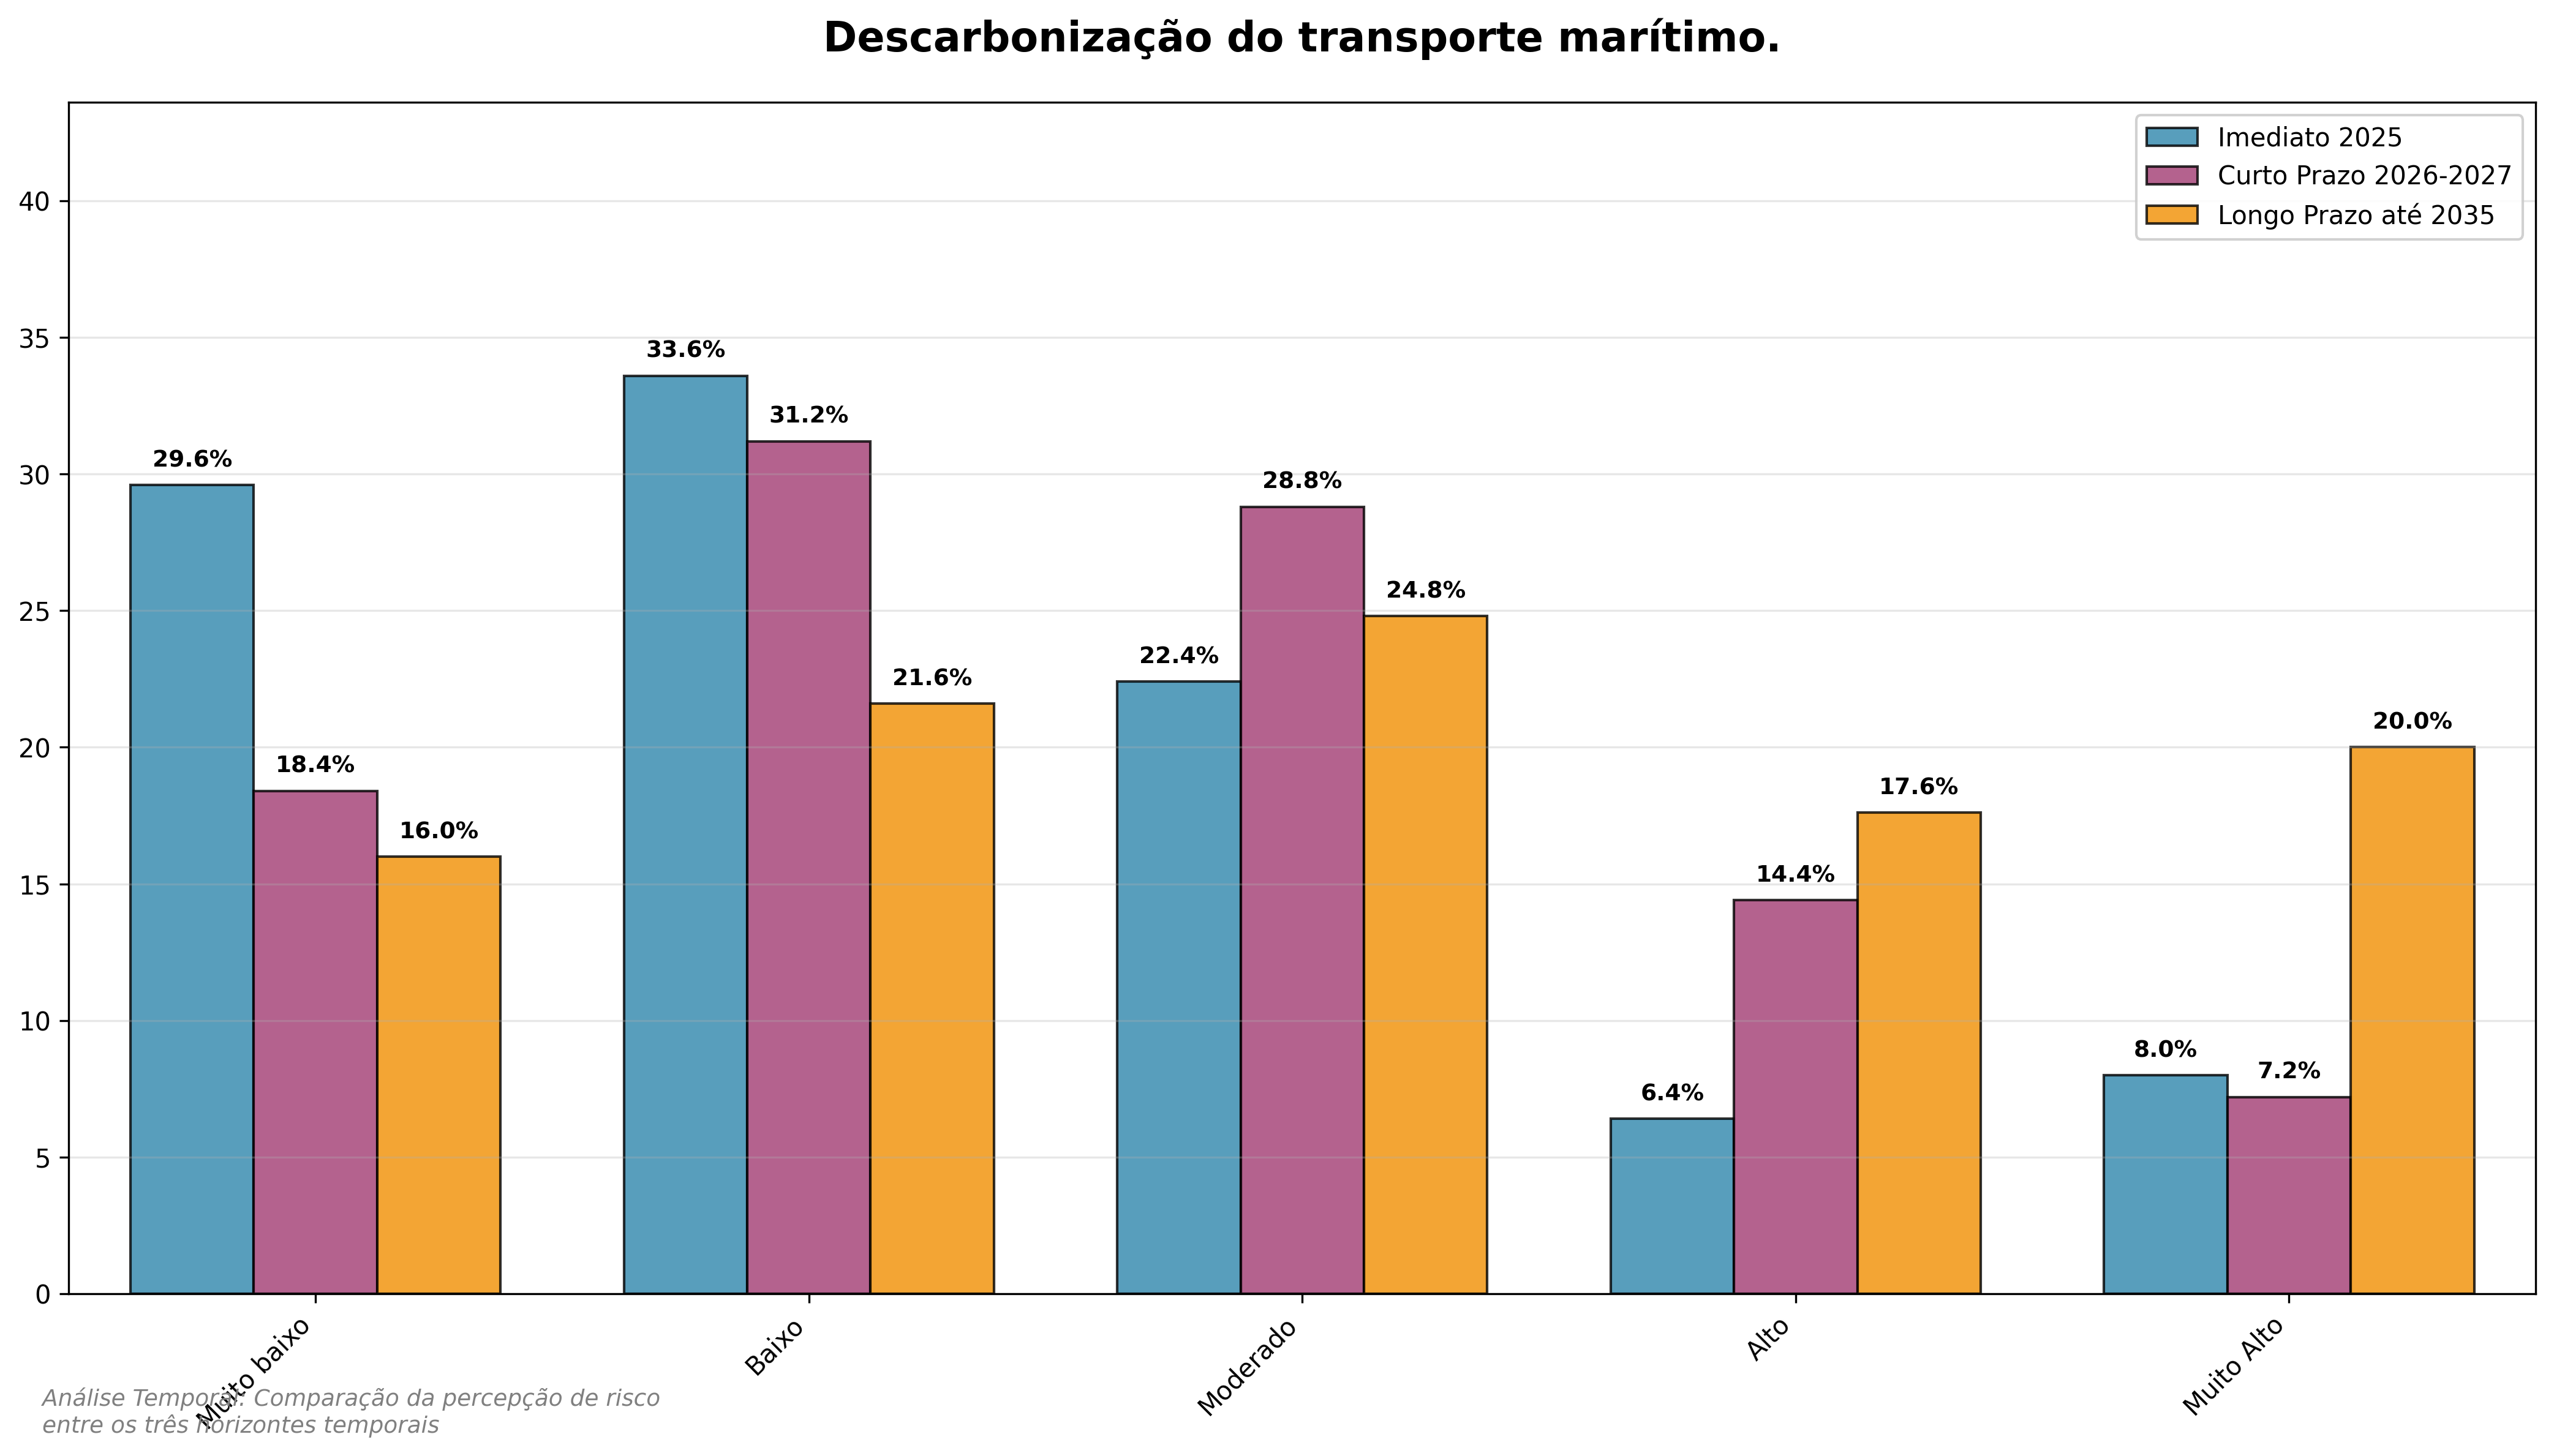
\includegraphics[keepaspectratio]{assets/ambientais/grafico_agrupado_2_16_temporal.png}}

\begin{tcolorbox}[enhanced jigsaw, titlerule=0mm, colback=white, title=\textcolor{quarto-callout-tip-color}{\faLightbulb}\hspace{0.5em}{Destaques}, opacityback=0, colbacktitle=quarto-callout-tip-color!10!white, leftrule=.75mm, left=2mm, colframe=quarto-callout-tip-color-frame, bottomrule=.15mm, bottomtitle=1mm, breakable, toprule=.15mm, toptitle=1mm, opacitybacktitle=0.6, arc=.35mm, coltitle=black, rightrule=.15mm]

\textbf{Evolução da Percepção de Risco:} Os dados evidenciam uma
tendência clara de aumento da percepção de risco associada à
descarbonização do setor, refletindo o reconhecimento crescente de que
as demandas regulatórias e comerciais por redução de emissões exigirão
transformações estruturais nas operações portuárias.

\textbf{Contexto Detalhado por Período:}

\textbf{Imediato (2025):} 14\% dos respondentes classificam o risco como
alto (4) ou muito alto (5) e mediana igual a 2. Nesse horizonte, o tema
é percebido como relevante, mas ainda distante da rotina operacional dos
portos.

\textbf{Curto Prazo (2026--2027):} 22\% em níveis 4-5 e mediana igual a
3. Observa-se crescimento da preocupação, alinhado à entrada em vigor de
novas regulamentações climáticas internacionais e à pressão de armadores
e clientes por operações mais limpas.

\textbf{Longo Prazo (até 2035):} 38\% em 4-5 e mediana igual a 3. A
percepção se intensifica de forma expressiva, revelando expectativa de
mudança estrutural profunda nas cadeias logísticas e na infraestrutura
energética portuária.

\textbf{Implicações Estratégicas:} As crescentes exigências regulatórias
e comerciais voltadas à descarbonização do transporte marítimo poderão
demandar transformação substancial nas operações portuárias, incluindo a
adoção de tecnologias de baixa emissão e integração de energias
renováveis. Entre as principais soluções estão o fornecimento de energia
em terra, a transição para combustíveis alternativos (hidrogênio,
amônia, biocombustíveis) e a eletrificação progressiva de equipamentos e
infraestruturas. Essas mudanças, embora fundamentais, ainda enfrentam
barreiras técnicas e financeiras, como altos custos de investimento,
falta de padronização global e disparidade na capacidade de adaptação
entre portos. Isso poderá gerar desafios operacionais e financeiros,
especialmente para portos de menor porte, impactando o planejamento
energético, a competitividade internacional e o alinhamento às metas
climáticas globais. Por outro lado, a adoção estratégica dessas
soluções, apoiada por inovação digital (IA, blockchain e sistemas
inteligentes de gestão energética) e cooperação entre atores públicos e
privados, pode consolidar o porto como referência em sustentabilidade e
liderança ambiental no cenário marítimo internacional, fortalecendo sua
resiliência e atratividade no longo prazo.

\end{tcolorbox}

\subsection{Baixa educação/conscientização
ambiental}\label{baixa-educauxe7uxe3oconscientizauxe7uxe3o-ambiental}

O gr?fico a seguir apresenta a evolu??o temporal do risco Baixa
educação/conscientização ambiental.
\pandocbounded{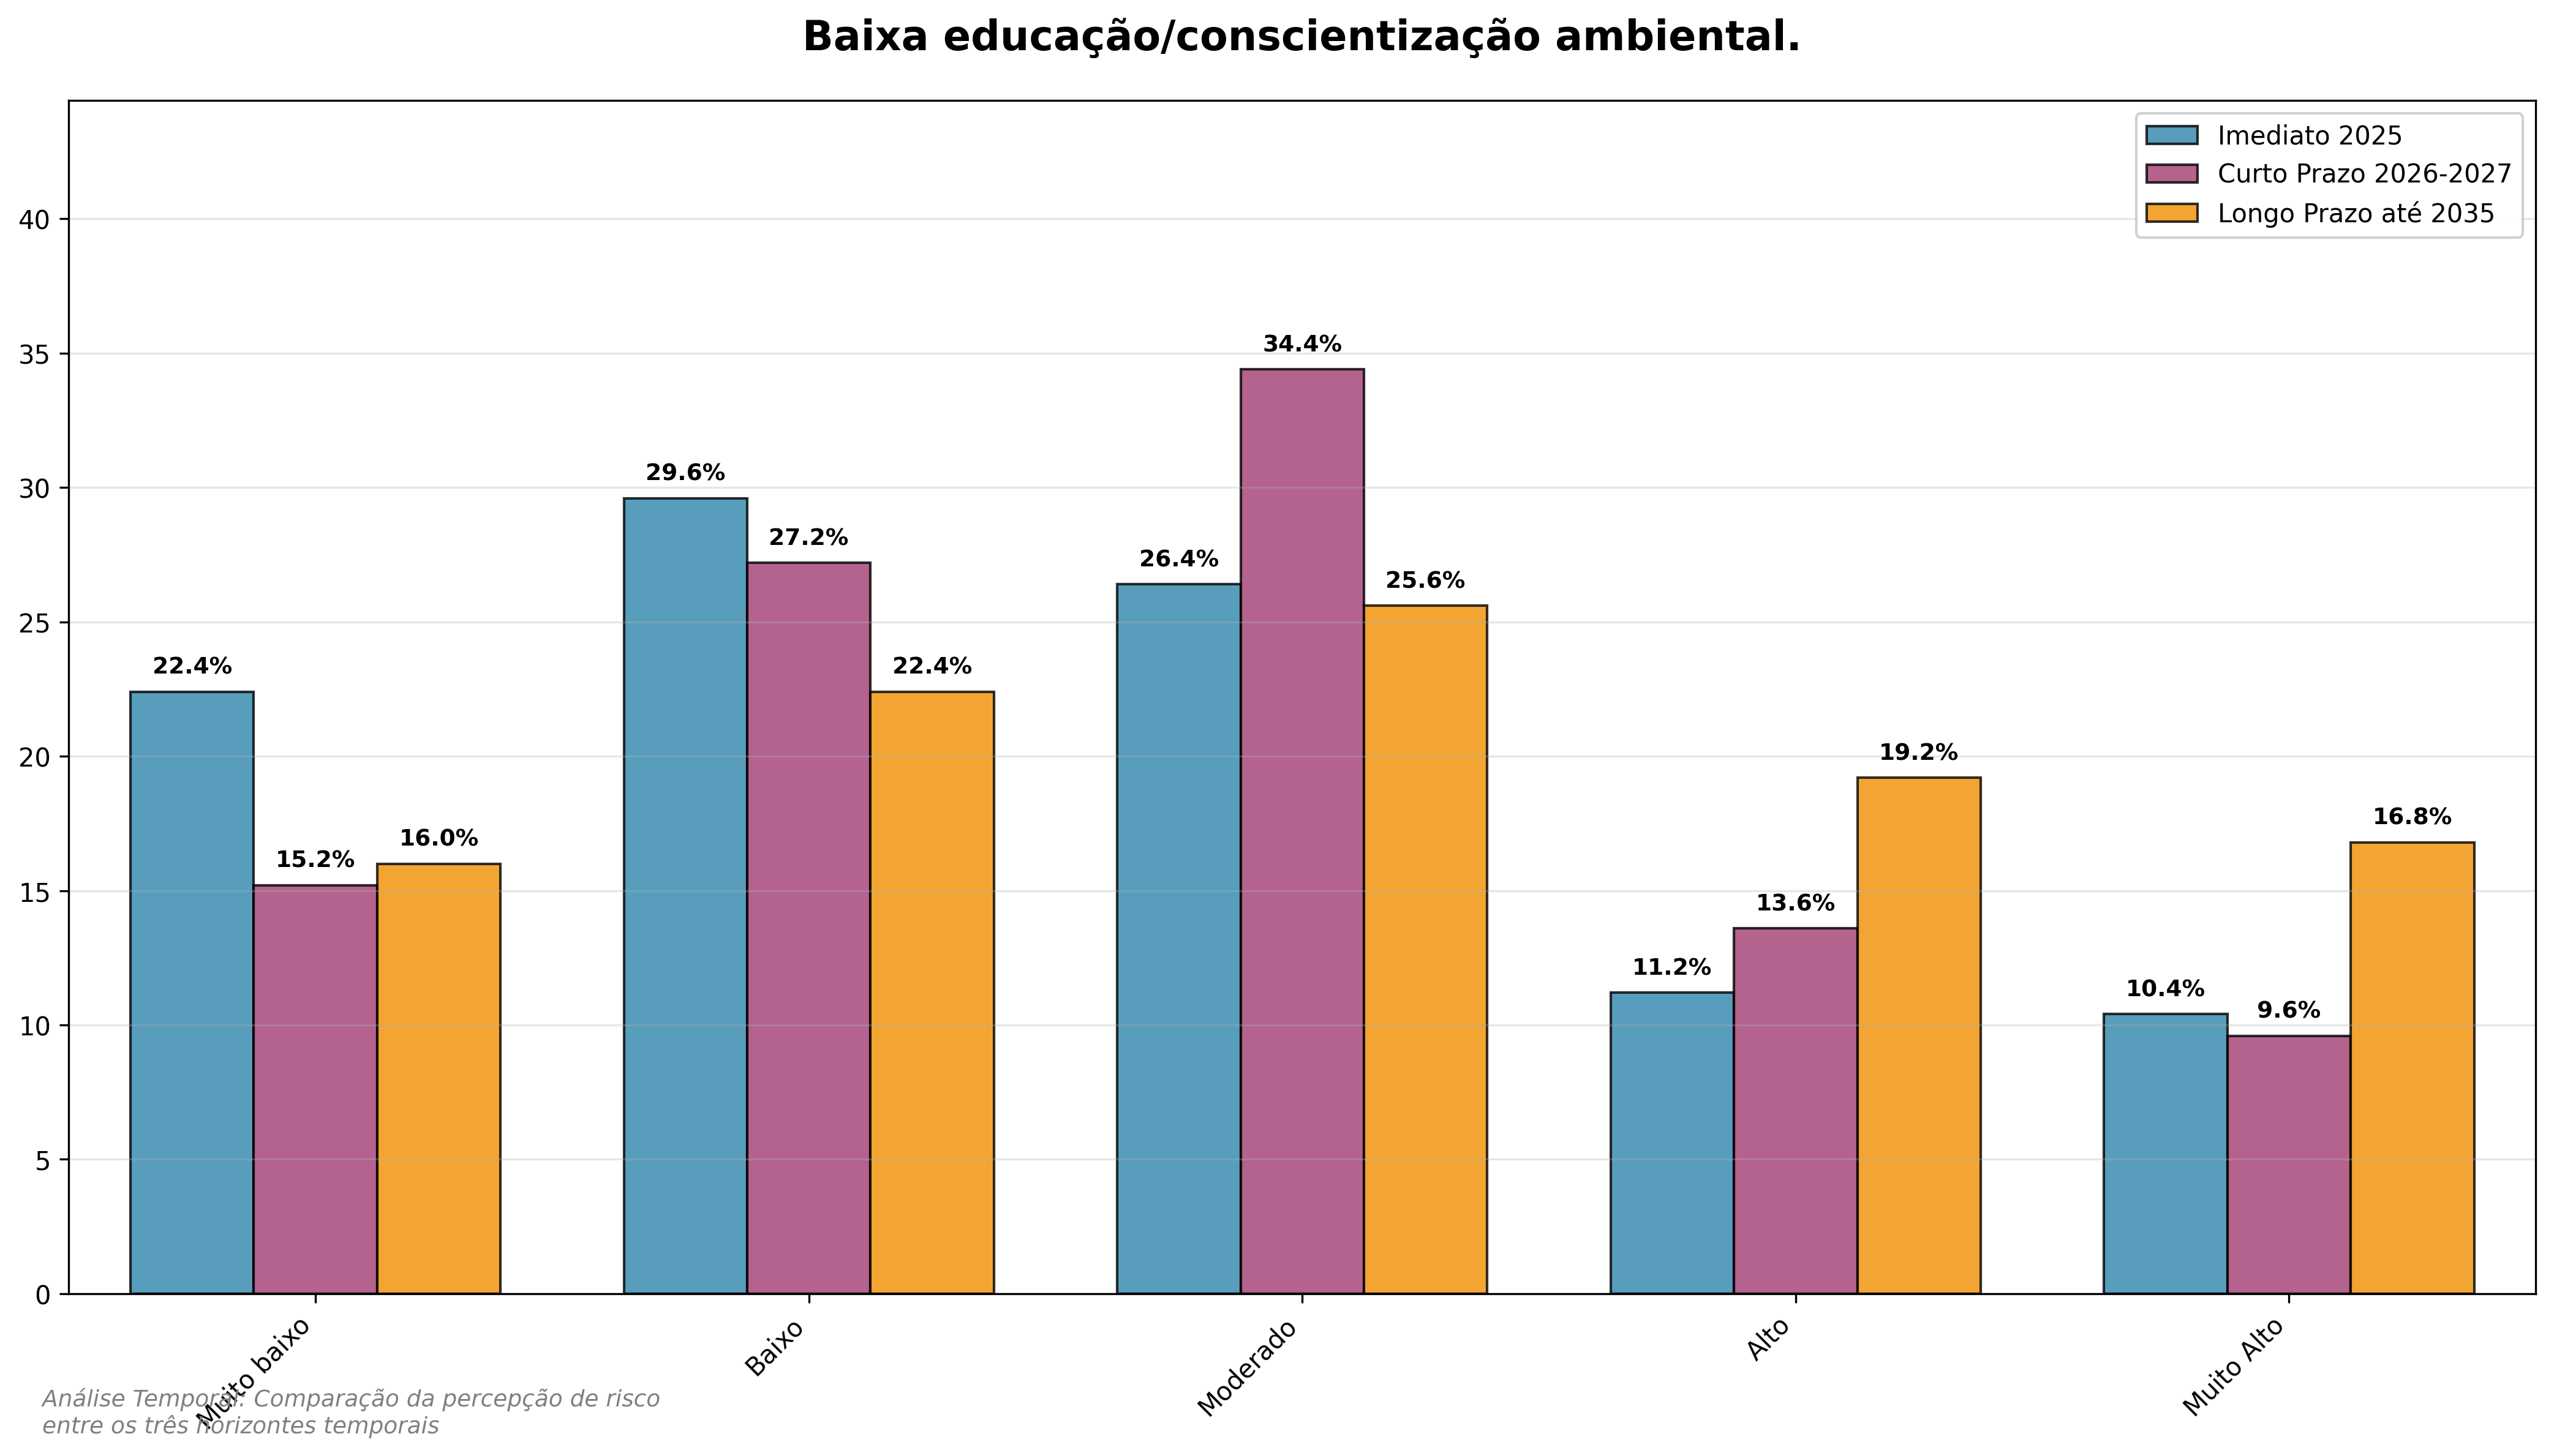
\includegraphics[keepaspectratio]{assets/ambientais/grafico_agrupado_2_17_temporal.png}}

\begin{tcolorbox}[enhanced jigsaw, titlerule=0mm, colback=white, title=\textcolor{quarto-callout-tip-color}{\faLightbulb}\hspace{0.5em}{Destaques}, opacityback=0, colbacktitle=quarto-callout-tip-color!10!white, leftrule=.75mm, left=2mm, colframe=quarto-callout-tip-color-frame, bottomrule=.15mm, bottomtitle=1mm, breakable, toprule=.15mm, toptitle=1mm, opacitybacktitle=0.6, arc=.35mm, coltitle=black, rightrule=.15mm]

\begin{longtable}[]{@{}
  >{\raggedright\arraybackslash}p{(\linewidth - 0\tabcolsep) * \real{1.0009}}@{}}
\toprule\noalign{}
\endhead
\bottomrule\noalign{}
\endlastfoot
\textbf{Evolução da Percepção de Risco:} O gráfico indica uma tendência
de aumento progressivo da percepção de risco associada à baixa educação
e conscientização ambiental entre trabalhadores, prestadores de serviço,
transportadores e demais integrantes da comunidade portuária ampliada.

\textbf{Contexto Detalhado por Período:}

\textbf{Imediato (2025):} 22\% dos respondentes classificam o risco como
alto (4) ou muito alto (5) e mediana igual a 2. O cenário imediato ainda
é de risco moderado. \textbar{}

\textbf{Curto Prazo (2026--2027):} 23\% em níveis 4-5 e mediana igual a
3. Observa-se aumento da preocupação, com destaque para a necessidade de
capacitação técnica e engajamento contínuo de colaboradores e parceiros
nas iniciativas de sustentabildade. \textbar{}

\textbf{Longo Prazo (até 2035):} 36\% em 4-5 e mediana igual a 3. A
percepção se intensifica significativamente, refletindo a compreensão de
que a sustentabilidade depende da consolidação de uma cultura
institucional voltada à responsabilidade socioambiental.

\textbf{Implicações Estratégicas:} A baixa educação e conscientização
ambiental pode gerar descumprimento de procedimentos ambientais,
descarte inadequado de resíduos e resistência à adoção de boas práticas
operacionais. Essas falhas aumentam o risco de incidentes ambientais
evitáveis, autuações regulatórias e desgaste da reputação institucional,
comprometendo tanto a governança ambiental quanto a imagem pública do
complexo portuário. Dentre as medidas recomendadas destacam-se:
implementação contínua de programas de educação e capacitação ambiental
para todos os níveis hierárquicos; inserção de metas de sustentabilidade
em planos de desempenho individual e institucional; campanhas de
sensibilização sobre boas práticas; criação de núcleos de
multiplicadores ambientais nos terminais e operadores; e estímulo à
comunicação transparente e participativa com a comunidade portuária.
Essas ações fortalecem a cultura de sustentabilidade, reduzem a
reincidência de não conformidades e consolidam o porto como agente
promotor de responsabilidade socioambiental. \\
\end{longtable}

\end{tcolorbox}

\section{Análise Temporal
Comparativa}\label{anuxe1lise-temporal-comparativa-1}

A análise comparativa entre os horizontes temporais revela importantes
padrões:

\subsection{Tendências
Identificadas}\label{tenduxeancias-identificadas-1}

\begin{itemize}
\tightlist
\item
  \textbf{Riscos Imediatos}: Maior preocupação com eventos climáticos
  extremos e desastres naturais;- \textbf{Riscos de Curto Prazo}:
  Destaque para escassez hídrica e poluição atmosférica;- \textbf{Riscos
  de Longo Prazo}: Preocupação crescente com aumento do nível do mar e
  descarbonização. \#\#\# Insights Estratégicos
\end{itemize}

\begin{enumerate}
\def\labelenumi{\arabic{enumi}.}
\tightlist
\item
  \textbf{Adaptação Climática}: Necessidade de investir em
  infraestrutura resiliente a eventos extremos;2. \textbf{Gestão
  Ambiental}: Implementar sistemas de monitoramento e controle;3.
  \textbf{Sustentabilidade}: Desenvolver práticas operacionais
  ambientalmente responsáveis;4. \textbf{Inovação Verde}: Investir em
  tecnologias limpas e processos sustentáveis. ::: \{.content-visible
  when-format=``docx''\}
\end{enumerate}

:::

\bookmarksetup{startatroot}

\chapter{Riscos Geopolíticos}\label{riscos-geopoluxedticos-1}

\section{Visão Geral dos Riscos
Geopolíticos}\label{visuxe3o-geral-dos-riscos-geopoluxedticos}

Os riscos geopolíticos foram avaliados em três horizontes temporais:

\begin{itemize}
\tightlist
\item
  \textbf{Imediato (2025)}: Riscos que requerem atenção imediata;-
  \textbf{Curto Prazo (2026-2027)}: Riscos emergentes que demandam
  planejamento;- \textbf{Longo Prazo (até 2035)}: Riscos estratégicos
  que requerem visão de futuro. \#\# Panorama do Período Imediato
\end{itemize}

O gr?fico a seguir mostra a distribui??o dos riscos no per?odo imediato.
\pandocbounded{\includegraphics[keepaspectratio]{assets/geopoliticos/grafico_barras_imediato_2025.png}}

\begin{tcolorbox}[enhanced jigsaw, titlerule=0mm, colback=white, title=\textcolor{quarto-callout-note-color}{\faInfo}\hspace{0.5em}{Destaques do período Imediato de 2025}, opacityback=0, colbacktitle=quarto-callout-note-color!10!white, leftrule=.75mm, left=2mm, colframe=quarto-callout-note-color-frame, bottomrule=.15mm, bottomtitle=1mm, breakable, toprule=.15mm, toptitle=1mm, opacitybacktitle=0.6, arc=.35mm, coltitle=black, rightrule=.15mm]

\begin{itemize}
\tightlist
\item
  \textbf{Conflitos geoeconômicos}: Mediana 3.0, 46\% das respostas em
  risco alto;
\item
  \textbf{Conflitos armados entre nações}: Mediana 2.0, 31\% em risco
  alto;
\item
  \textbf{Violência em países parceiros}: Mediana 2.0, 28\% em risco
  alto.
\end{itemize}

\end{tcolorbox}

\section{Análise Temporal da Dimensão
Geopolítica}\label{anuxe1lise-temporal-da-dimensuxe3o-geopoluxedtica}

O gr?fico a seguir sintetiza a evolu??o temporal das vari?veis da
dimens?o geopol?tica.
\pandocbounded{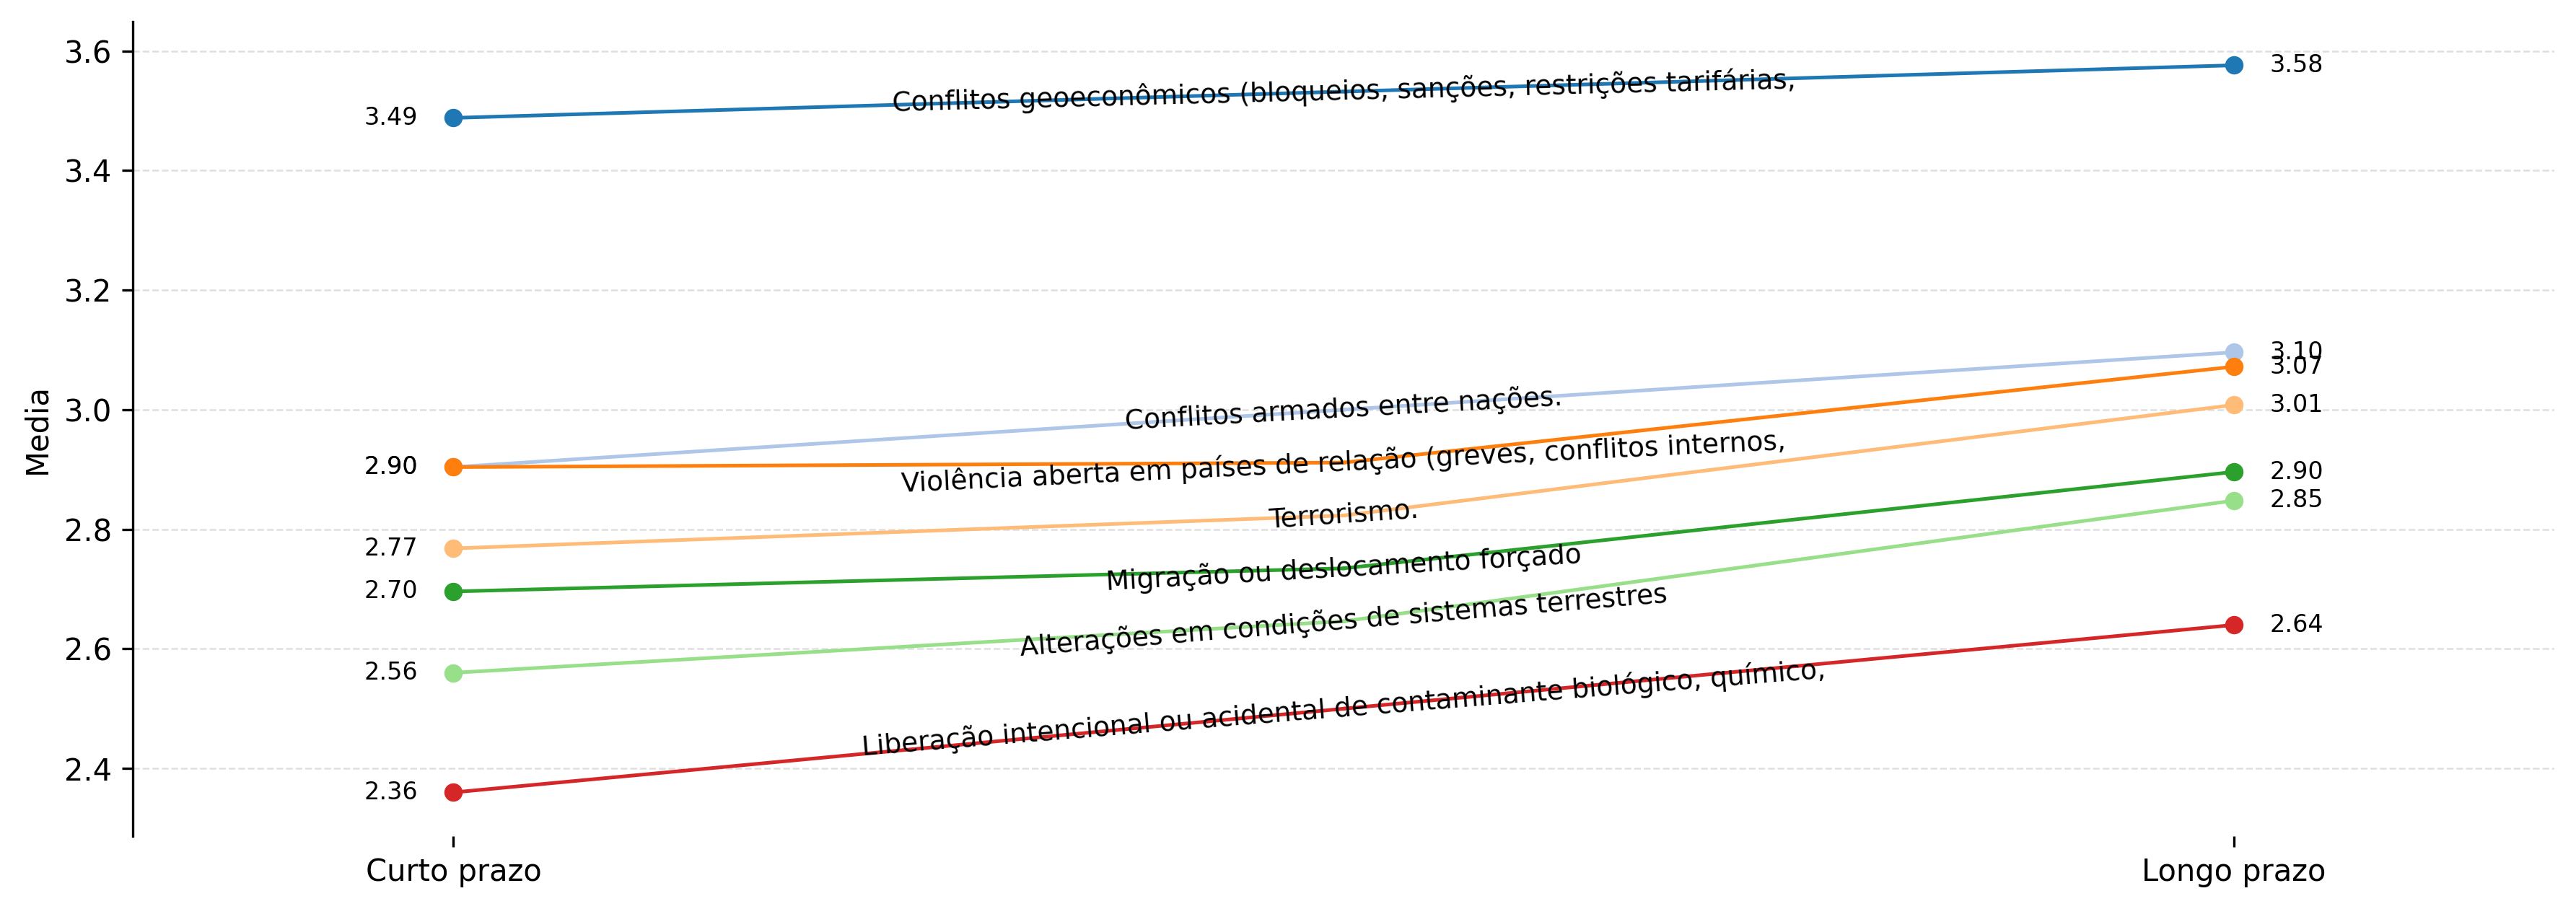
\includegraphics[keepaspectratio]{assets/slopegraphs_por_dimensao/slopegraph_geopolítica.png}}

\begin{tcolorbox}[enhanced jigsaw, titlerule=0mm, colback=white, title=\textcolor{quarto-callout-note-color}{\faInfo}\hspace{0.5em}{Destaques da Evolução Temporal}, opacityback=0, colbacktitle=quarto-callout-note-color!10!white, leftrule=.75mm, left=2mm, colframe=quarto-callout-note-color-frame, bottomrule=.15mm, bottomtitle=1mm, breakable, toprule=.15mm, toptitle=1mm, opacitybacktitle=0.6, arc=.35mm, coltitle=black, rightrule=.15mm]

\begin{itemize}
\tightlist
\item
  \textbf{Conflitos geoeconômicos}: Mediana evolui de 3.0 (46\% em risco
  alto) para 4.0 (60\%) no longo prazo;
\item
  \textbf{Conflitos armados}: Percentual em risco alto sobe de 31\% para
  44\% entre 2025 e 2035;
\item
  \textbf{Terrorismo}: Risco alto cresce de 30\% para 41\%, exigindo
  reforços constantes de segurança.
\end{itemize}

\end{tcolorbox}

Embora com menor número de variáveis (5), os riscos geopolíticos
demonstram alta relevância, com trajetórias temporais distintas que
refletem a volatilidade do cenário internacional e seu impacto direto
nas operações portuárias.

\subsection{Insights da Análise Temporal
Geopolítica}\label{insights-da-anuxe1lise-temporal-geopoluxedtica}

A análise temporal dos riscos geopolíticos revela padrões de
volatilidade e crescente preocupação:

\subsubsection{Piora Geopolítica
Moderada}\label{piora-geopoluxedtica-moderada}

\begin{itemize}
\item
  \textbf{Delta médio de +0,40}: Segunda maior piora entre as
  dimensões;- \textbf{2 variáveis com piora crítica (+1.0 ponto)}:
  Terrorismo, liberação de agentes biológicos;- \textbf{Tendência de
  deterioração consistente}: A maioria dos riscos mostra piora
  progressiva. \#\#\#\# Padrões Específicos Identificados
\item
  \textbf{Conflitos Geoeconômicos como Principal Risco}: Mantém-se
  persistentemente alto em todos os períodos;- \textbf{Instabilidade
  Política Crescente}: Evolui de mediana 3.0 para 4.0, tornando-se
  crítica;- \textbf{Segurança Portuária em Ascensão}: Terrorismo e
  pirataria mostram piora significativa. \#\#\#\# Destaques da Evolução
  Temporal
\item
  \textbf{Risco Mais Crítico em 2035}: Instabilidade política em países
  parceiros (60\% em risco alto);- \textbf{Maior Crescimento Relativo}:
  Terrorismo (+34\% no risco alto);- \textbf{Transformação da
  Segurança}: Pirataria e crimes marítimos (+34\% no risco alto).
  \#\#\#\# Implicações Estratégicas para a Dimensão Geopolítica
\end{itemize}

A análise temporal geopolítica exige vigilância contínua:

\begin{enumerate}
\def\labelenumi{\arabic{enumi}.}
\tightlist
\item
  \textbf{Monitoramento Estratégico}: Implementar sistema de
  inteligência geopolítica em tempo real;2. \textbf{Diversificação de
  Rotas e Parcerias}: Reduzir dependência de regiões instáveis;3.
  \textbf{Fortalecimento da Segurança}: Investir em tecnologias e
  protocolos antiterrorismo;4. \textbf{Planejamento de Contingência}:
  Desenvolver cenários de resposta a crises geopolíticas. \#\# Exame das
  Variáveis de Risco: Resultados e Tendências
\end{enumerate}

\subsection{Liberação intencional ou acidental de
contaminantes}\label{liberauxe7uxe3o-intencional-ou-acidental-de-contaminantes}

O gr?fico a seguir apresenta a evolu??o temporal do risco Liberação
intencional ou acidental de contaminantes.
\pandocbounded{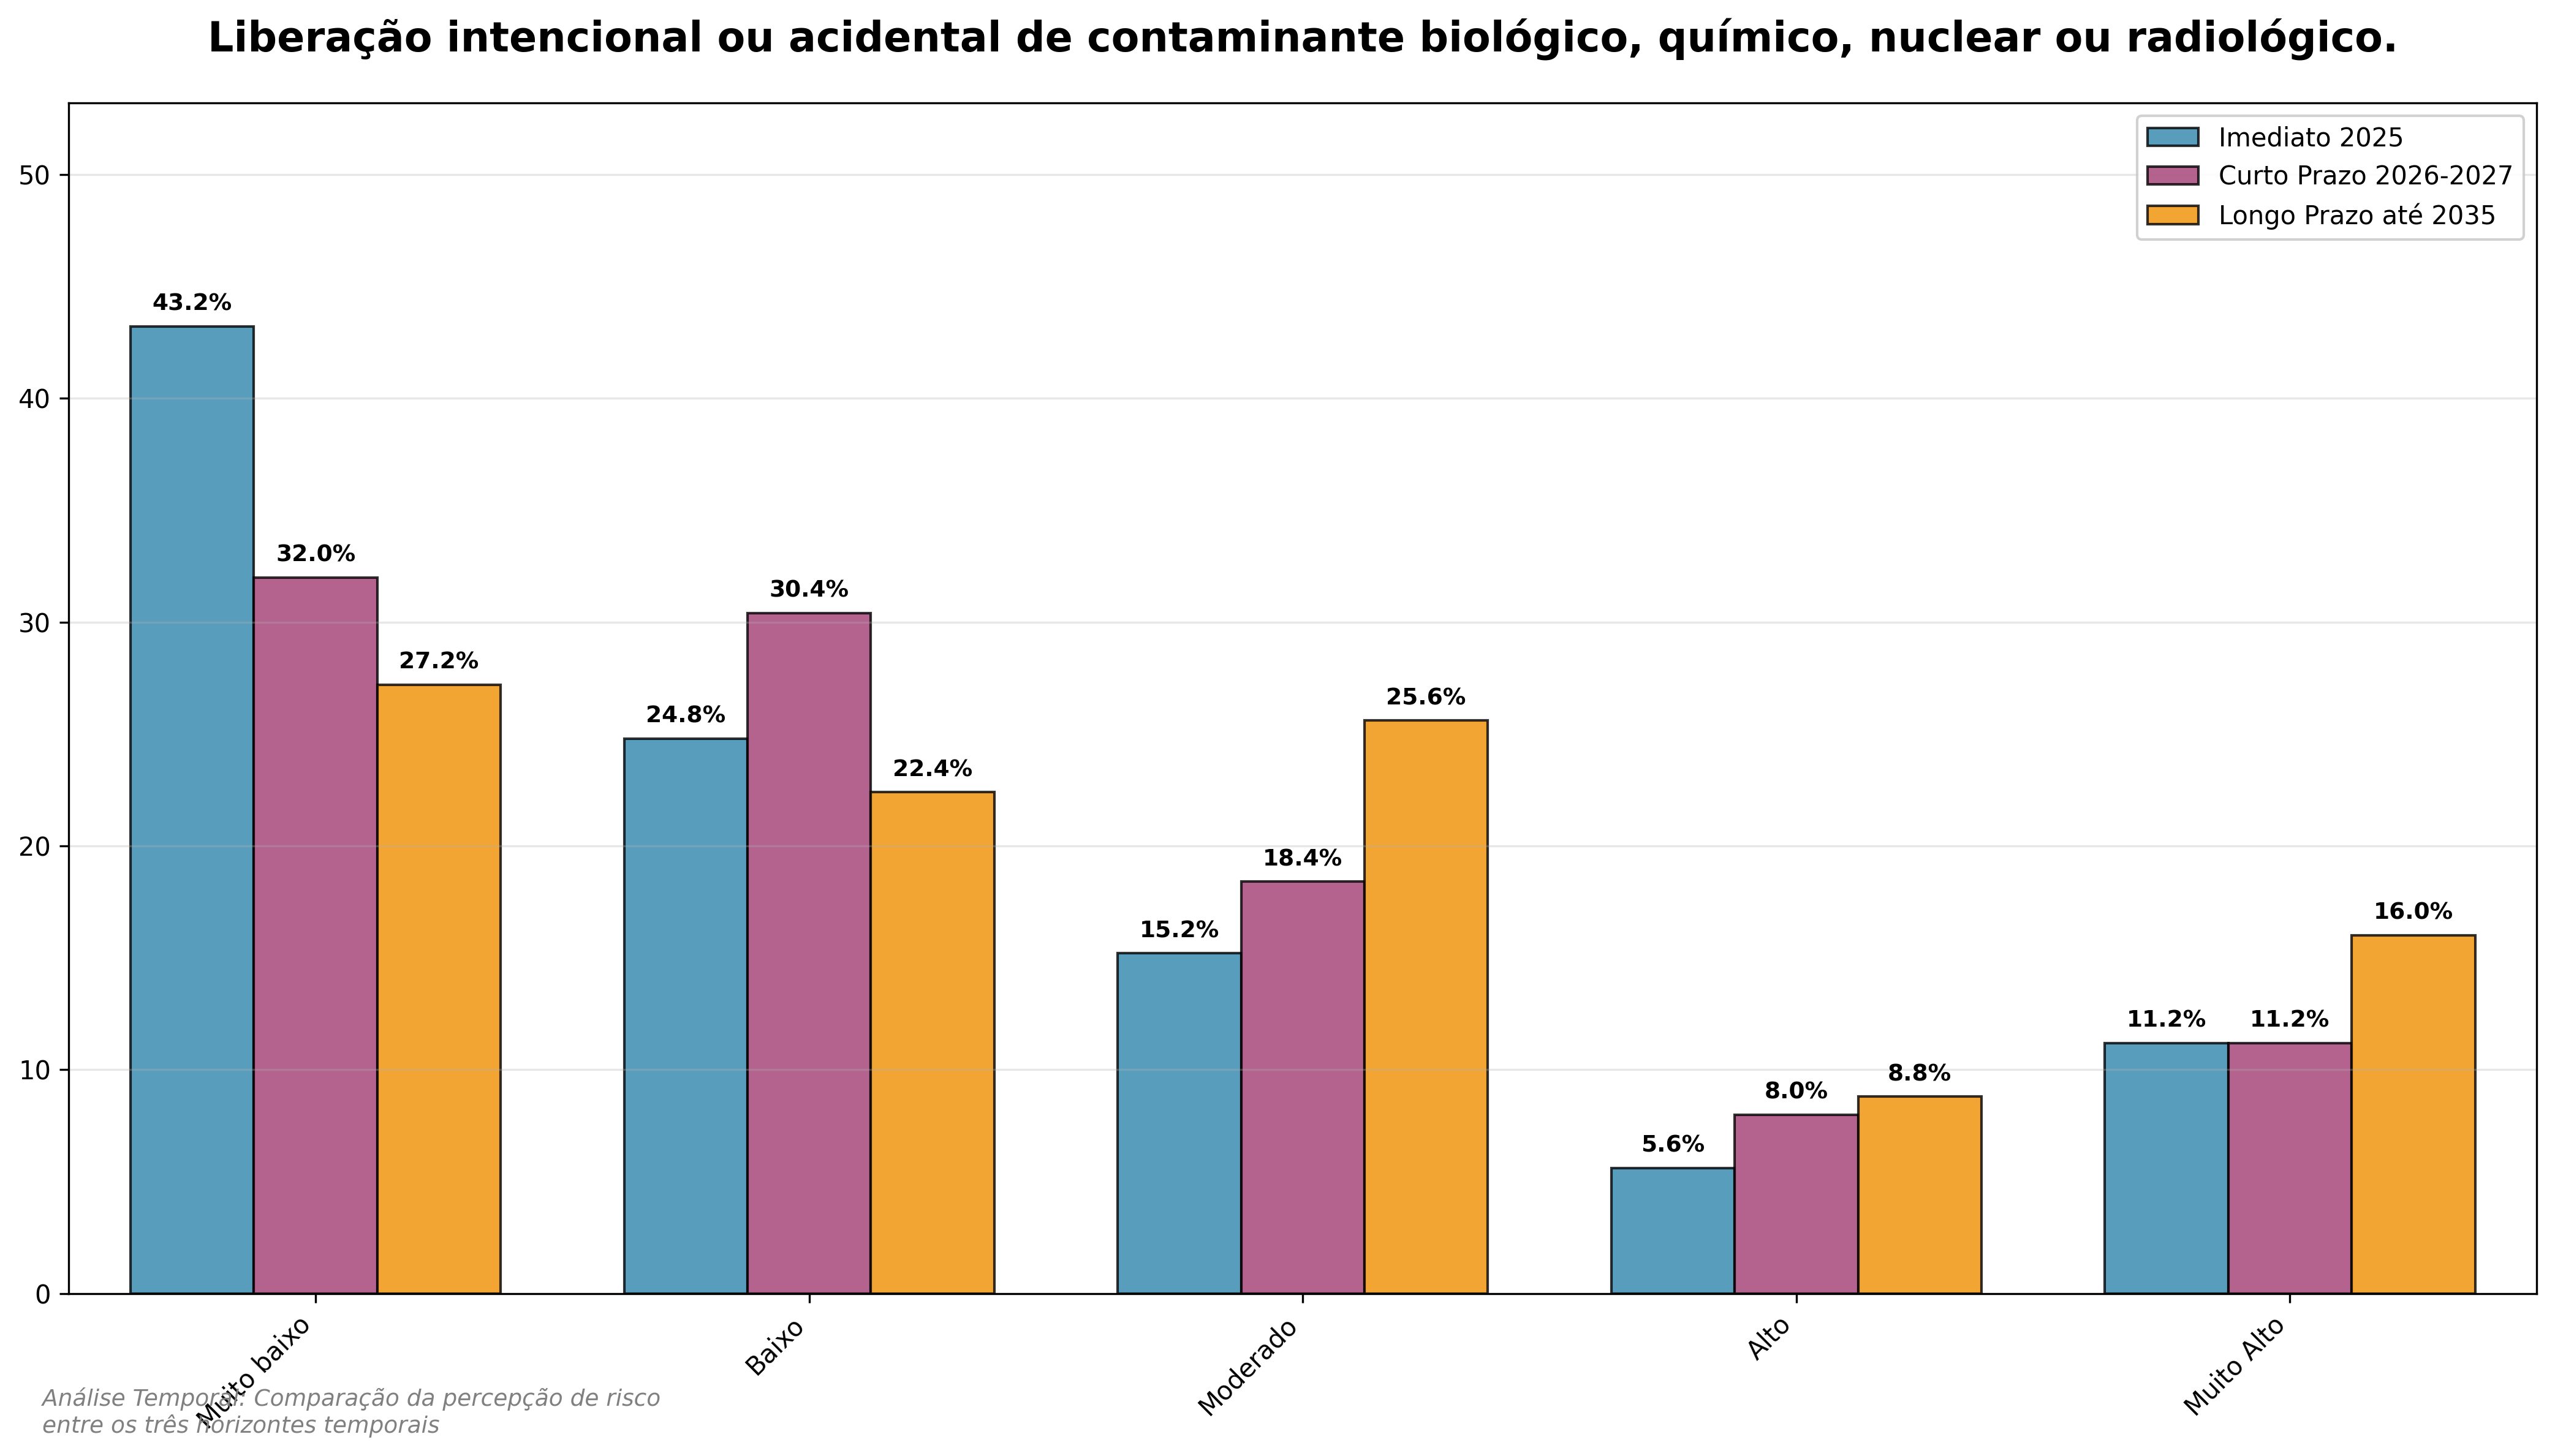
\includegraphics[keepaspectratio]{assets/geopoliticos/grafico_agrupado_3_1_temporal.png}}

\begin{tcolorbox}[enhanced jigsaw, titlerule=0mm, colback=white, title=\textcolor{quarto-callout-tip-color}{\faLightbulb}\hspace{0.5em}{Destaques}, opacityback=0, colbacktitle=quarto-callout-tip-color!10!white, leftrule=.75mm, left=2mm, colframe=quarto-callout-tip-color-frame, bottomrule=.15mm, bottomtitle=1mm, breakable, toprule=.15mm, toptitle=1mm, opacitybacktitle=0.6, arc=.35mm, coltitle=black, rightrule=.15mm]

\textbf{Imediato (2025)}: Mediana 2.0, 17\% em risco alto

\textbf{Curto Prazo (2026-2027)}: Mediana 2.0, 19\% em risco alto

\textbf{Longo Prazo (até 2035)}: Mediana 3.0, 25\% em risco alto

Devido à possibilidade de liberação intencional ou acidental de
contaminantes de natureza biológica, química, nuclear ou radiológica,
poderá ocorrer interrupção de operações portuárias e imposição de
restrições sanitárias emergenciais, o que poderá levar a perdas
econômicas e logísticas significativas, impactando a segurança
operacional, a continuidade dos serviços e a confiança dos parceiros
comerciais internacionais.

\end{tcolorbox}

\subsection{Alterações em condições de sistemas
terrestres}\label{alterauxe7uxf5es-em-condiuxe7uxf5es-de-sistemas-terrestres}

O gr?fico a seguir apresenta a evolu??o temporal do risco Alterações em
condições de sistemas terrestres.
\pandocbounded{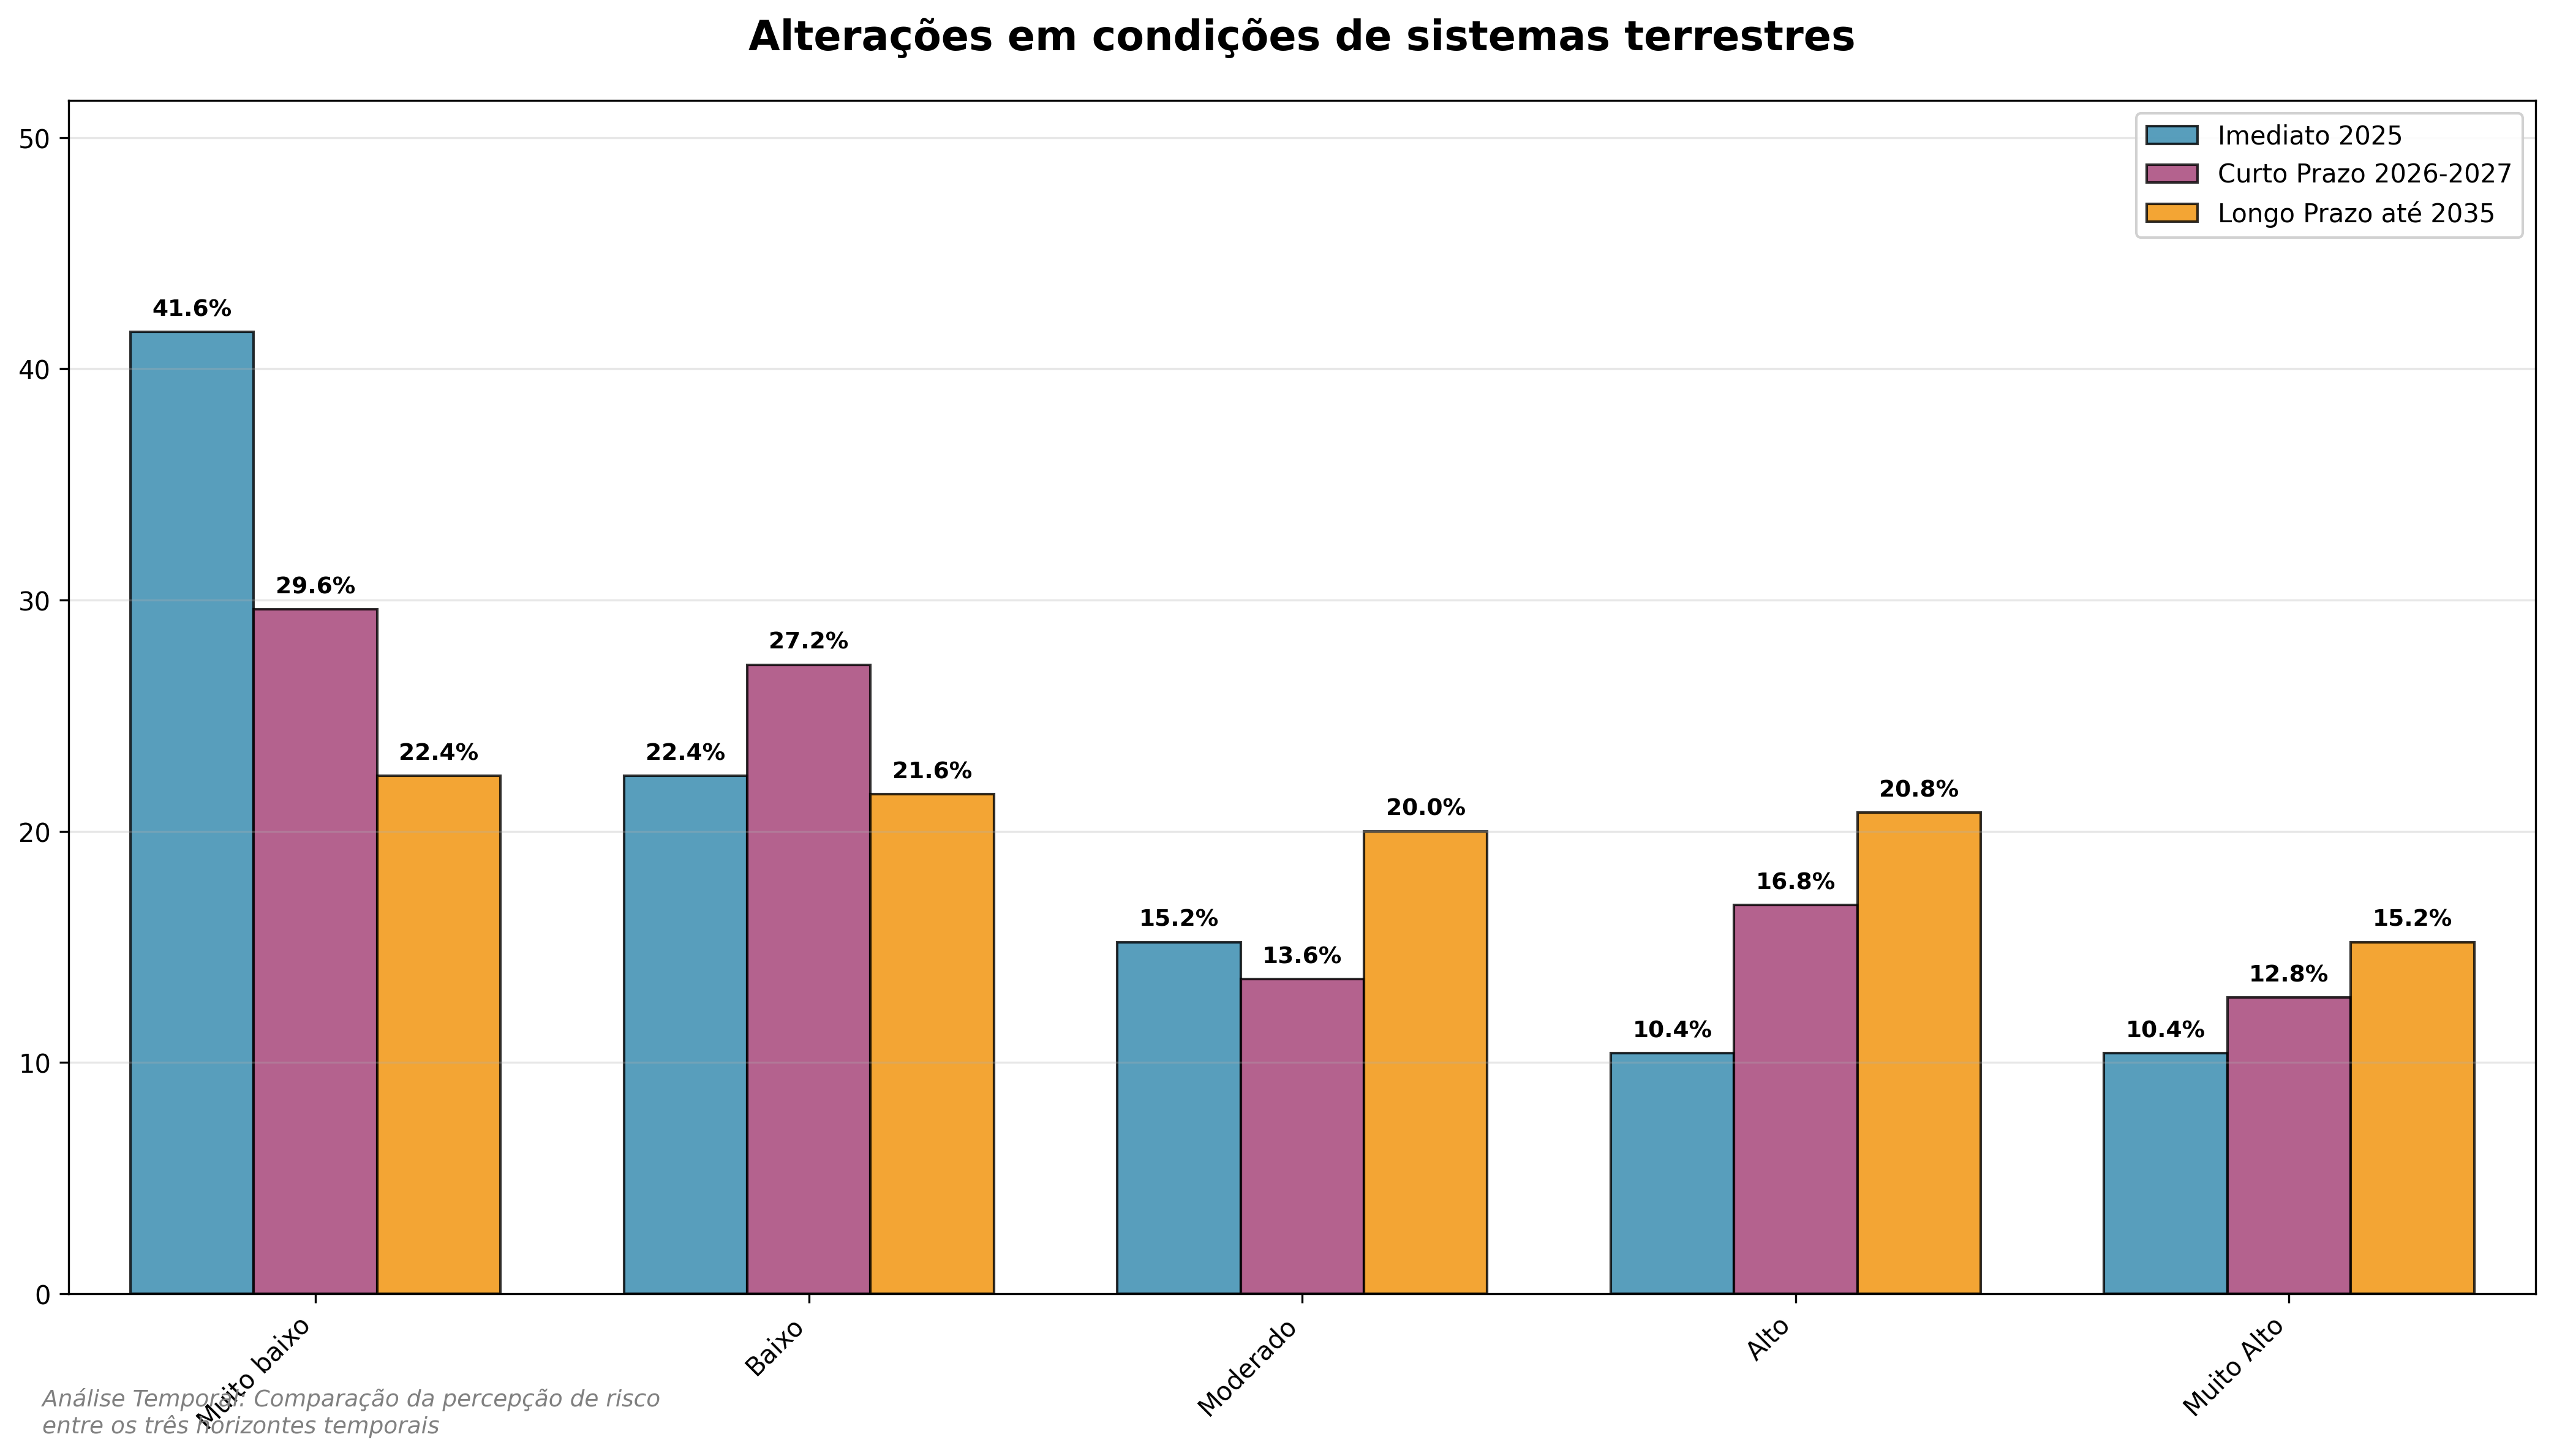
\includegraphics[keepaspectratio]{assets/geopoliticos/grafico_agrupado_3_2_temporal.png}}

\begin{tcolorbox}[enhanced jigsaw, titlerule=0mm, colback=white, title=\textcolor{quarto-callout-tip-color}{\faLightbulb}\hspace{0.5em}{Destaques}, opacityback=0, colbacktitle=quarto-callout-tip-color!10!white, leftrule=.75mm, left=2mm, colframe=quarto-callout-tip-color-frame, bottomrule=.15mm, bottomtitle=1mm, breakable, toprule=.15mm, toptitle=1mm, opacitybacktitle=0.6, arc=.35mm, coltitle=black, rightrule=.15mm]

\textbf{Imediato (2025)}: Mediana 2.0, 21\% em risco alto

\textbf{Curto Prazo (2026-2027)}: Mediana 2.0, 30\% em risco alto

\textbf{Longo Prazo (até 2035)}: Mediana 3.0, 36\% em risco alto

Devido a disputas por soberania em áreas estratégicas, redefinições de
fronteiras e controle de recursos naturais, poderá acontecer restrição
de acesso a rotas comerciais e aumento de tensões diplomáticas
regionais, o que poderá levar a reorientações logísticas e aumento de
custos de transporte, impactando a competitividade internacional e a
estabilidade das cadeias de suprimento portuárias.

\end{tcolorbox}

\subsection{Conflitos econômicos em países parceiros
comerciais}\label{conflitos-econuxf4micos-em-pauxedses-parceiros-comerciais}

O gr?fico a seguir apresenta a evolu??o temporal do risco Conflitos
econômicos em países parceiros comerciais.
\pandocbounded{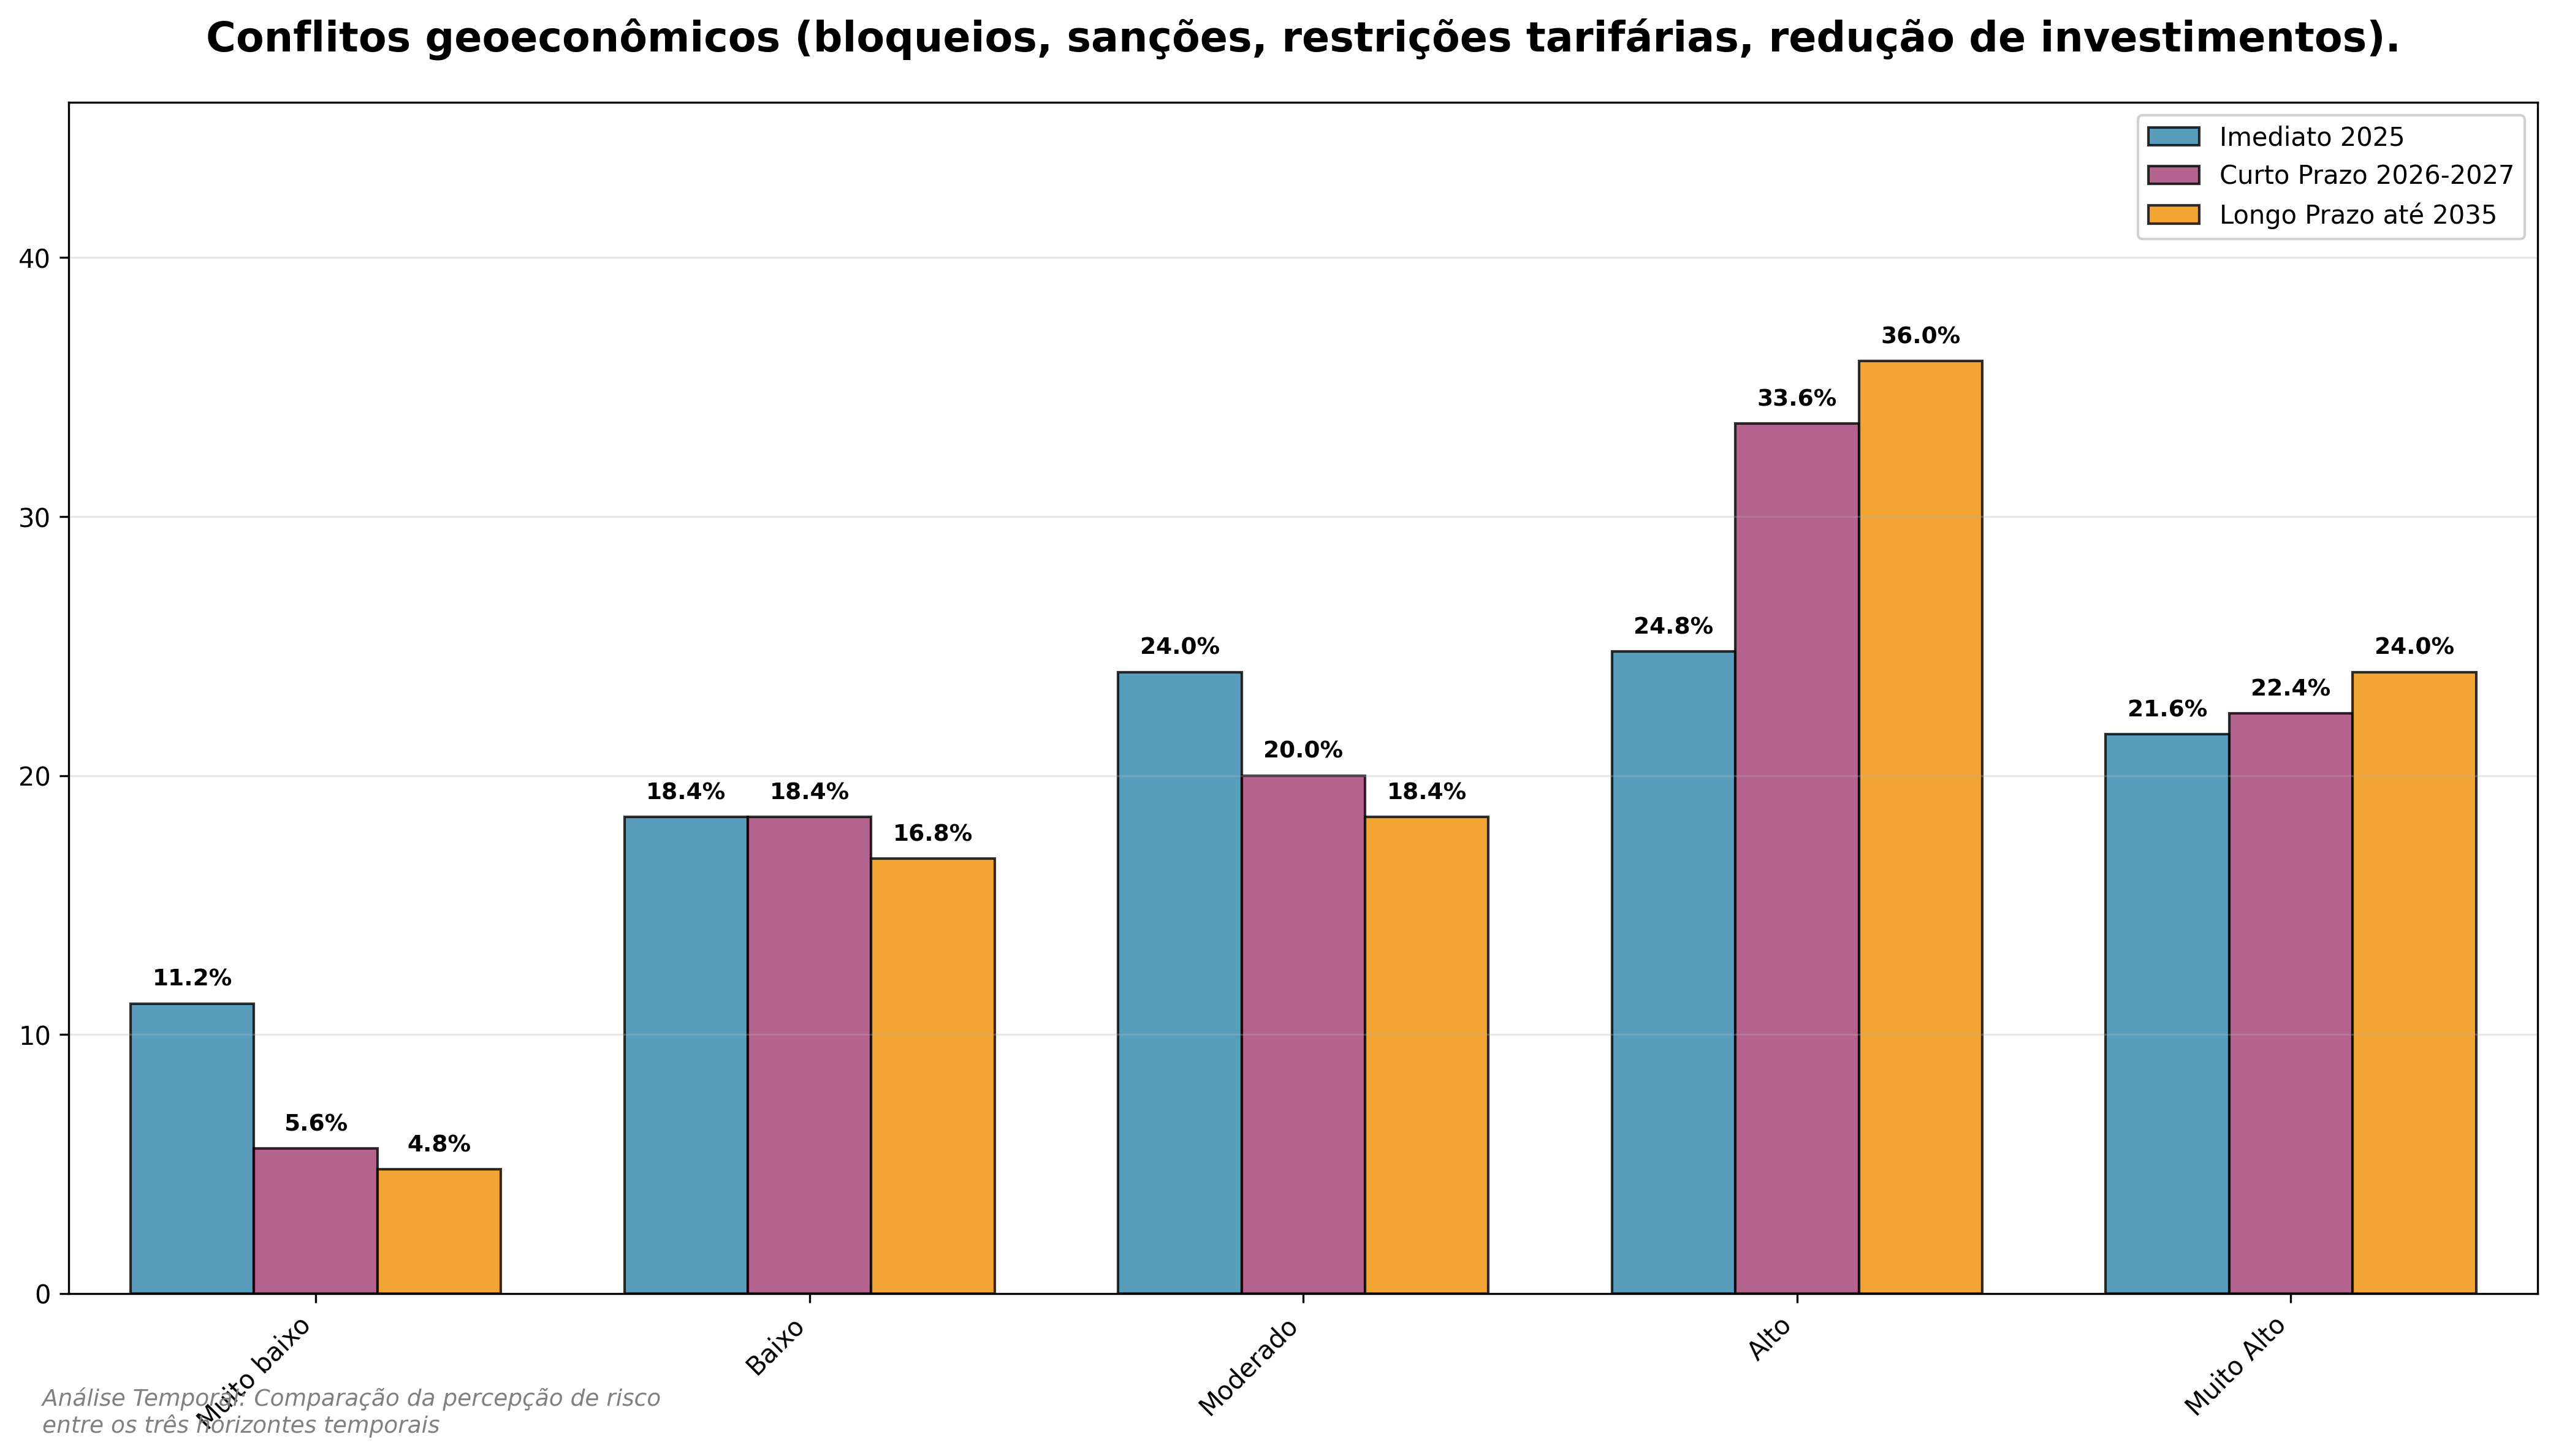
\includegraphics[keepaspectratio]{assets/geopoliticos/grafico_agrupado_3_3_temporal.png}}

\begin{tcolorbox}[enhanced jigsaw, titlerule=0mm, colback=white, title=\textcolor{quarto-callout-tip-color}{\faLightbulb}\hspace{0.5em}{Destaques}, opacityback=0, colbacktitle=quarto-callout-tip-color!10!white, leftrule=.75mm, left=2mm, colframe=quarto-callout-tip-color-frame, bottomrule=.15mm, bottomtitle=1mm, breakable, toprule=.15mm, toptitle=1mm, opacitybacktitle=0.6, arc=.35mm, coltitle=black, rightrule=.15mm]

\textbf{Imediato (2025)}: Mediana 3.0, 46\% em risco alto

\textbf{Curto Prazo (2026-2027)}: Mediana 4.0, 56\% em risco alto

\textbf{Longo Prazo (até 2035)}: Mediana 4.0, 60\% em risco alto

Devido à intensificação de bloqueios comerciais, sanções econômicas e
redução de investimentos estrangeiros, poderá ocorrer restrição de
fluxos comerciais e elevação da volatilidade cambial, o que poderá levar
a desequilíbrios na logística internacional e redução da atratividade de
novos empreendimentos, impactando a sustentabilidade financeira e a
inserção internacional do setor portuário brasileiro.

\end{tcolorbox}

\subsection{Conflitos armados entre
nações}\label{conflitos-armados-entre-nauxe7uxf5es}

O gr?fico a seguir apresenta a evolu??o temporal do risco Conflitos
armados entre nações.
\pandocbounded{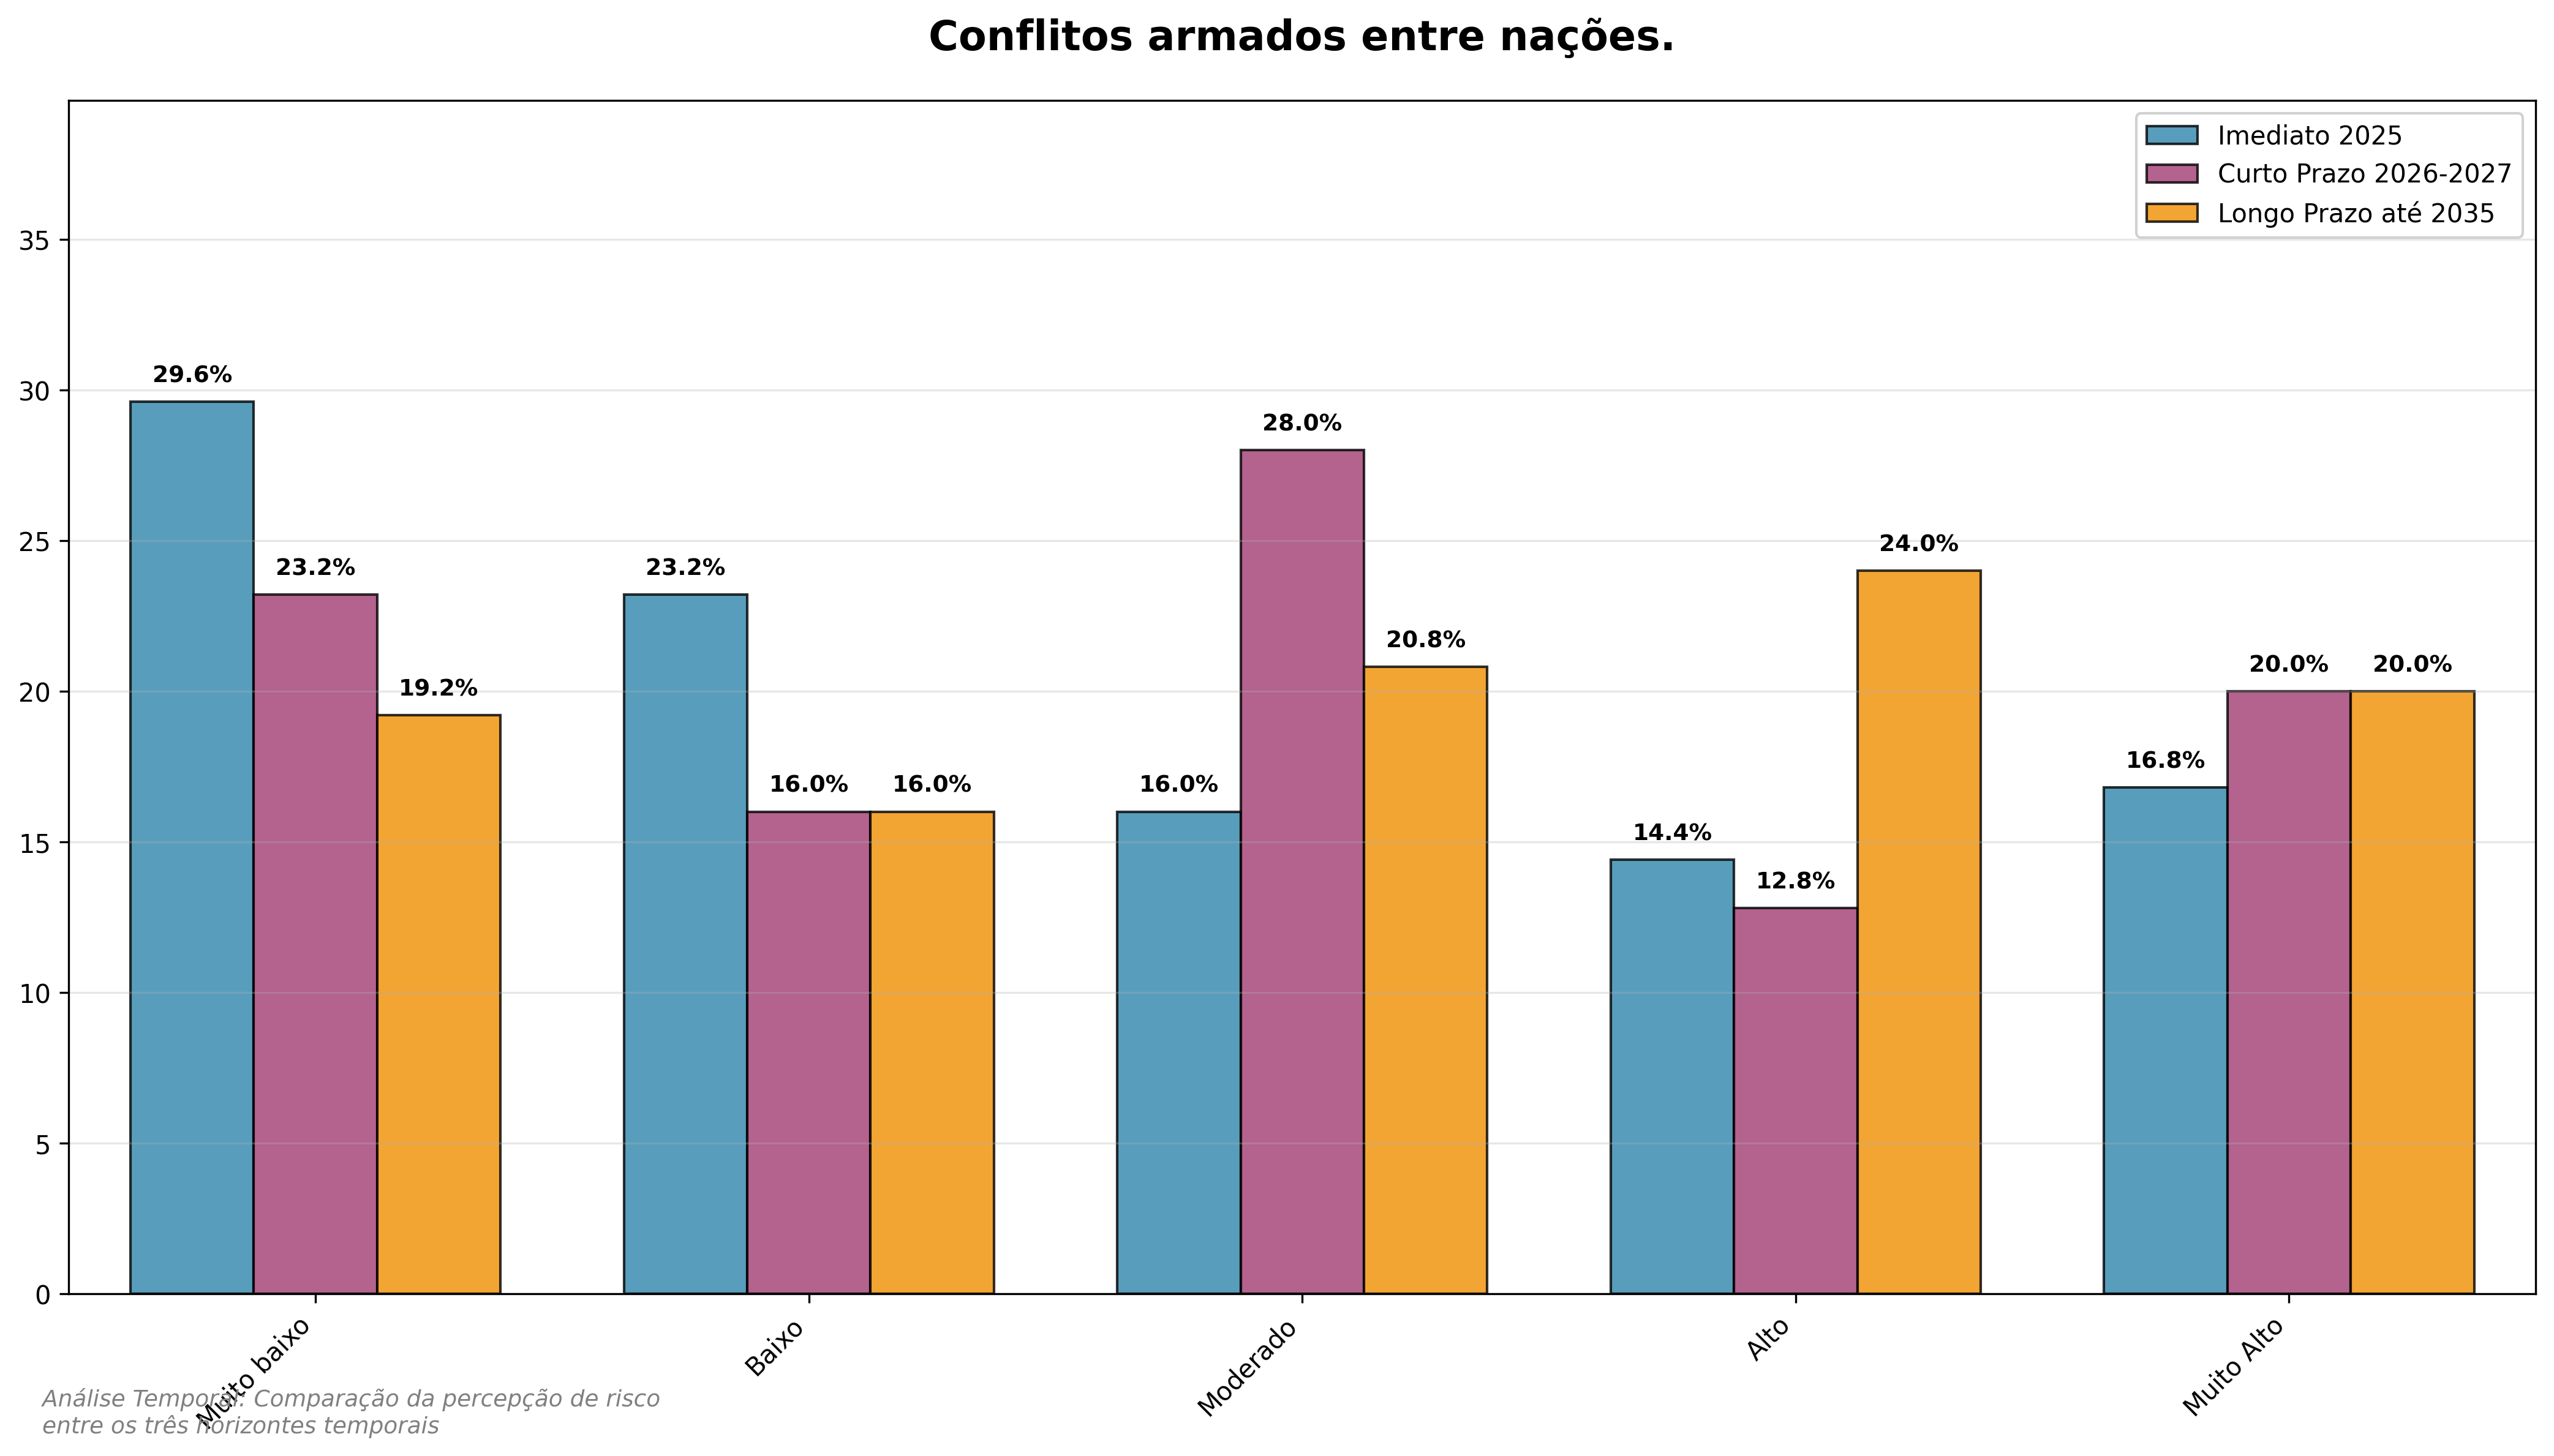
\includegraphics[keepaspectratio]{assets/geopoliticos/grafico_agrupado_3_4_temporal.png}}

\begin{tcolorbox}[enhanced jigsaw, titlerule=0mm, colback=white, title=\textcolor{quarto-callout-tip-color}{\faLightbulb}\hspace{0.5em}{Destaques}, opacityback=0, colbacktitle=quarto-callout-tip-color!10!white, leftrule=.75mm, left=2mm, colframe=quarto-callout-tip-color-frame, bottomrule=.15mm, bottomtitle=1mm, breakable, toprule=.15mm, toptitle=1mm, opacitybacktitle=0.6, arc=.35mm, coltitle=black, rightrule=.15mm]

\textbf{Imediato (2025)}: Mediana 2.0, 31\% em risco alto

\textbf{Curto Prazo (2026-2027)}: Mediana 3.0, 33\% em risco alto

\textbf{Longo Prazo (até 2035)}: Mediana 3.0, 44\% em risco alto

Devido à possibilidade de escalada de tensões e confrontos militares
entre Estados, poderá ocorrer interrupção de rotas marítimas
estratégicas e aumento expressivo dos custos de seguros e fretes, o que
poderá levar a deslocamento de fluxos comerciais e fragilização de
cadeias críticas, impactando a segurança energética, alimentar e
logística nacional.

\end{tcolorbox}

\subsection{Violência interna em países parceiros (greves, conflitos
internos, golpes de Estado, insegurança
pública)}\label{violuxeancia-interna-em-pauxedses-parceiros-greves-conflitos-internos-golpes-de-estado-inseguranuxe7a-puxfablica}

O gr?fico a seguir apresenta a evolu??o temporal do risco Violência
interna em países parceiros (greves, conflitos internos, golpes de
Estado, insegurança pública).
\pandocbounded{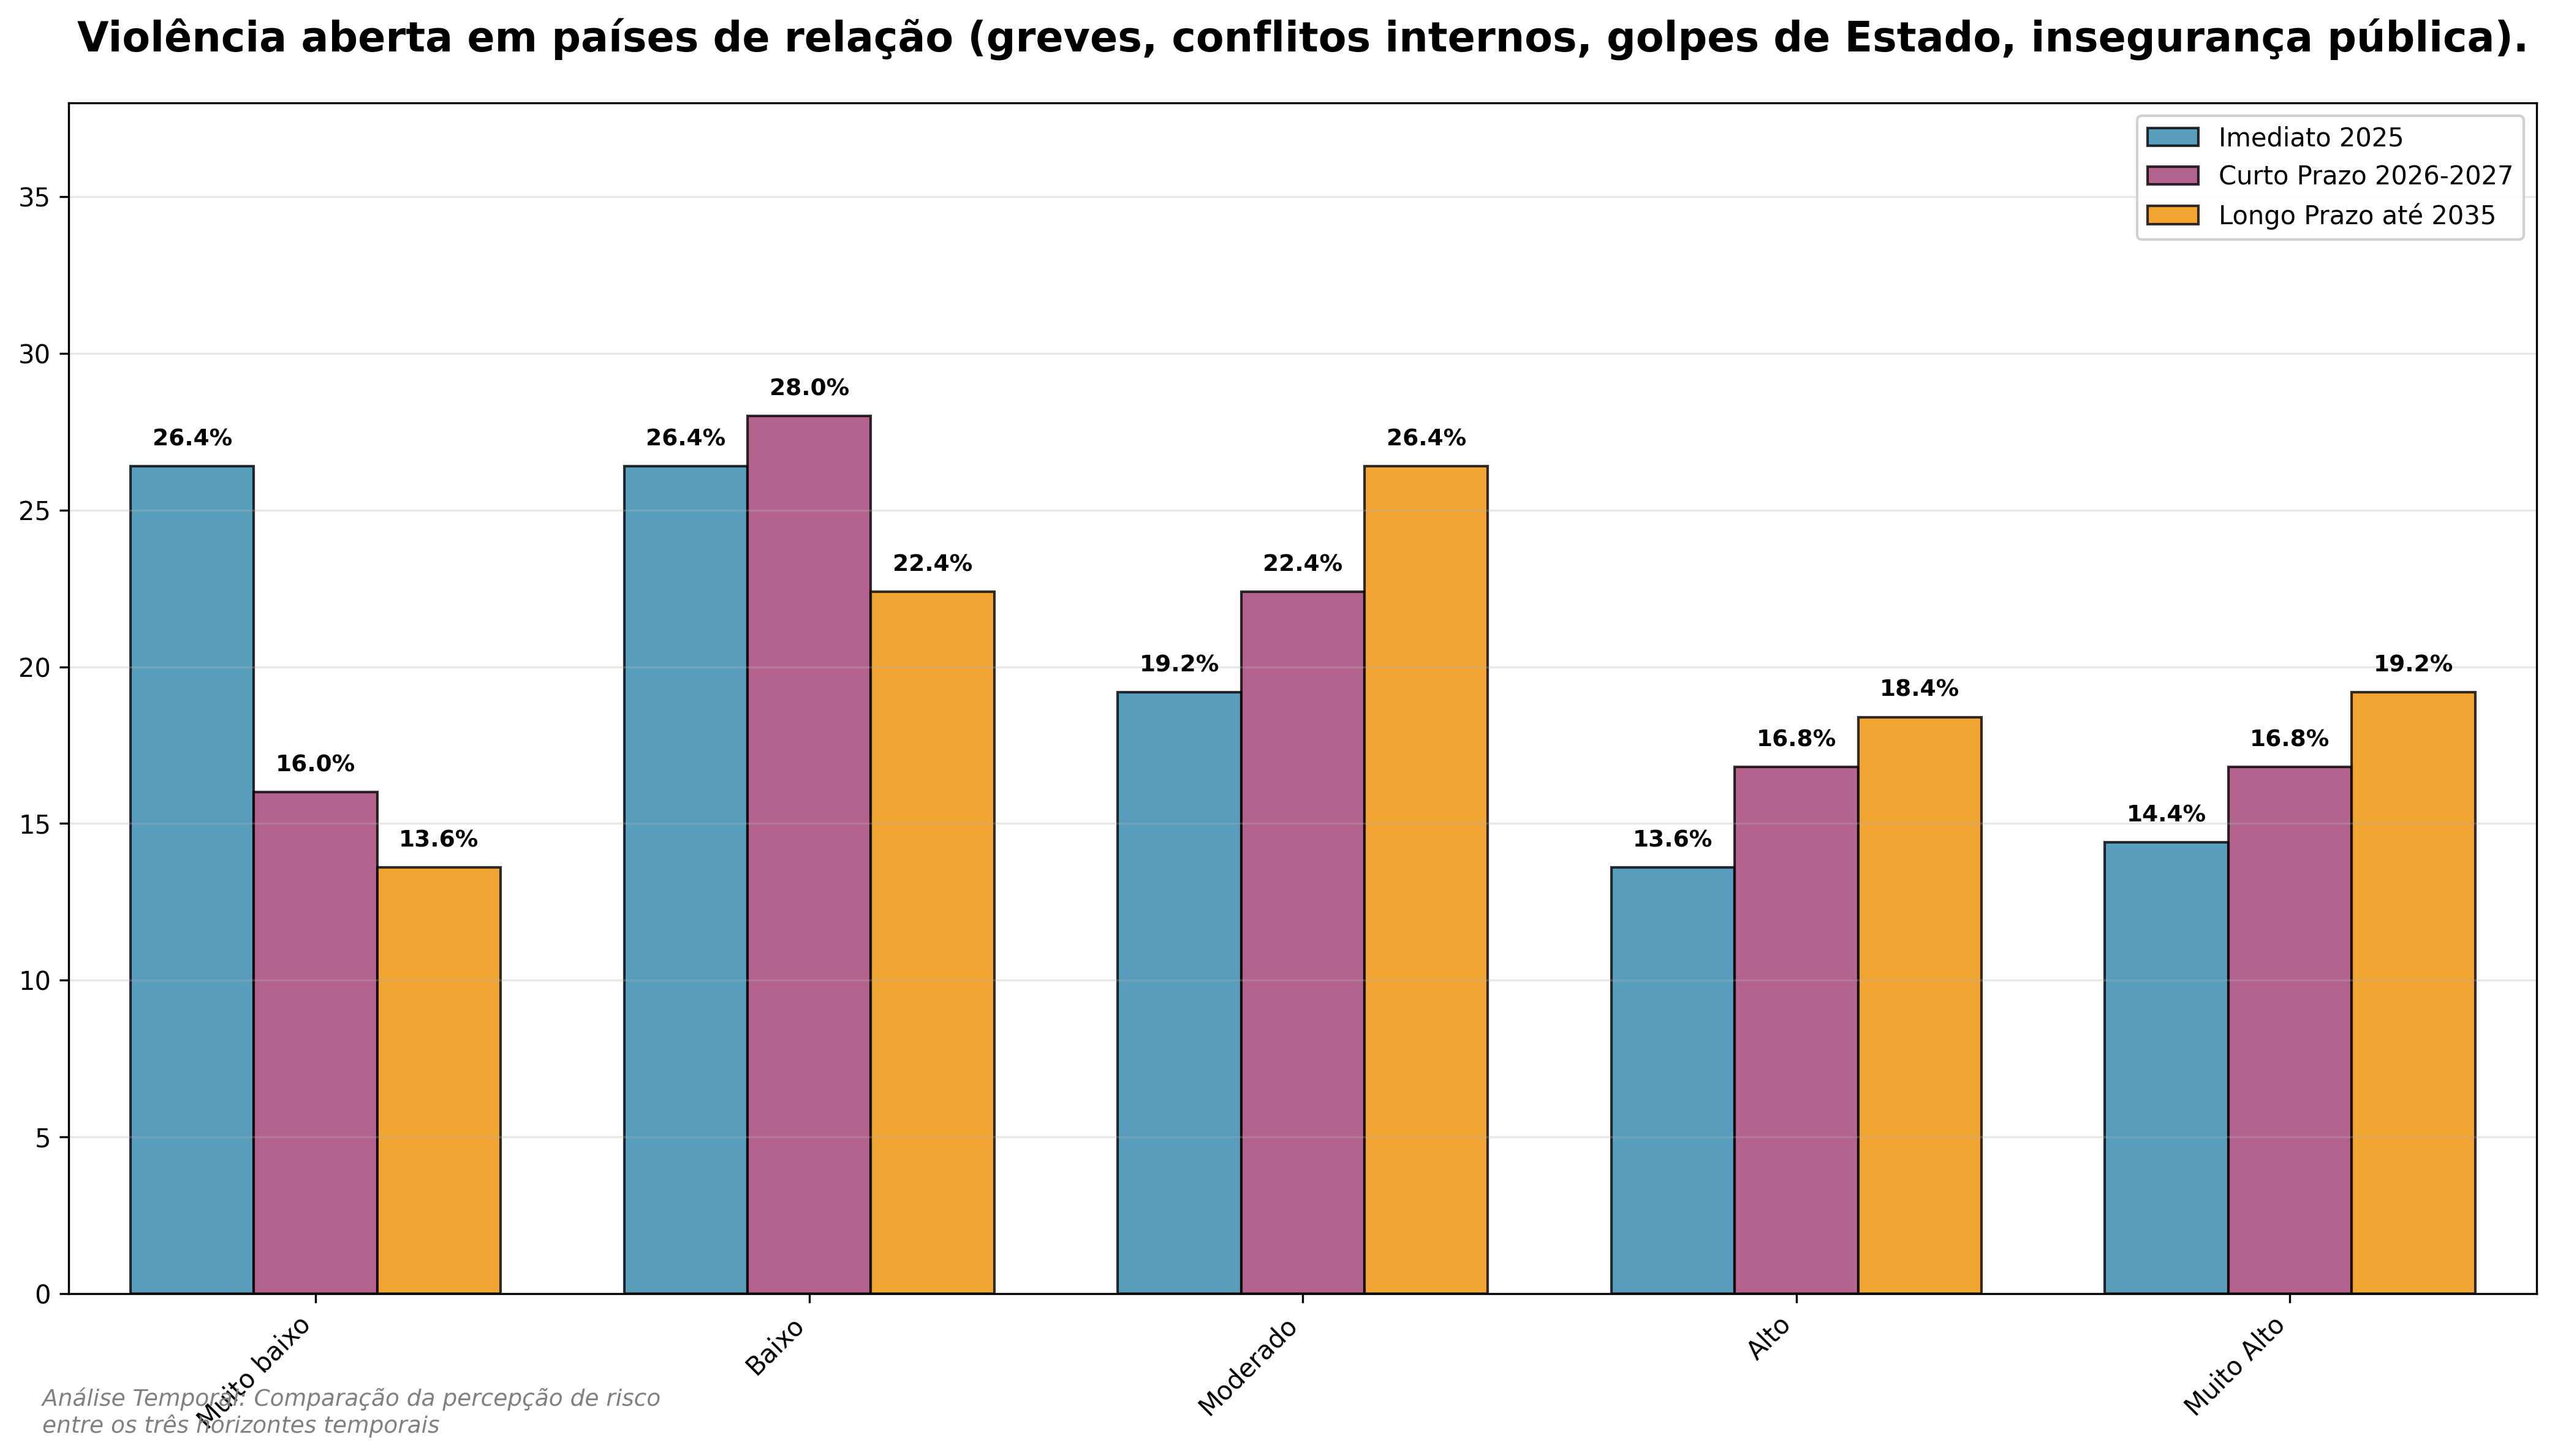
\includegraphics[keepaspectratio]{assets/geopoliticos/grafico_agrupado_3_5_temporal.png}}

\begin{tcolorbox}[enhanced jigsaw, titlerule=0mm, colback=white, title=\textcolor{quarto-callout-tip-color}{\faLightbulb}\hspace{0.5em}{Destaques}, opacityback=0, colbacktitle=quarto-callout-tip-color!10!white, leftrule=.75mm, left=2mm, colframe=quarto-callout-tip-color-frame, bottomrule=.15mm, bottomtitle=1mm, breakable, toprule=.15mm, toptitle=1mm, opacitybacktitle=0.6, arc=.35mm, coltitle=black, rightrule=.15mm]

\textbf{Imediato (2025)}: Mediana 2.0, 28\% em risco alto

\textbf{Curto Prazo (2026-2027)}: Mediana 3.0, 34\% em risco alto

\textbf{Longo Prazo (até 2035)}: Mediana 3.0, 38\% em risco alto

Devido à instabilidade política e social em países parceiros comerciais,
poderá acontecer interrupção de exportações, greves em terminais
logísticos e elevação de riscos de segurança operacional, o que poderá
levar a atrasos e aumento de custos operacionais, impactando a
confiabilidade, eficiência e imagem institucional do sistema portuário
brasileiro

\end{tcolorbox}

\subsection{Terrorismo}\label{terrorismo}

O gr?fico a seguir apresenta a evolu??o temporal do risco Terrorismo.
\pandocbounded{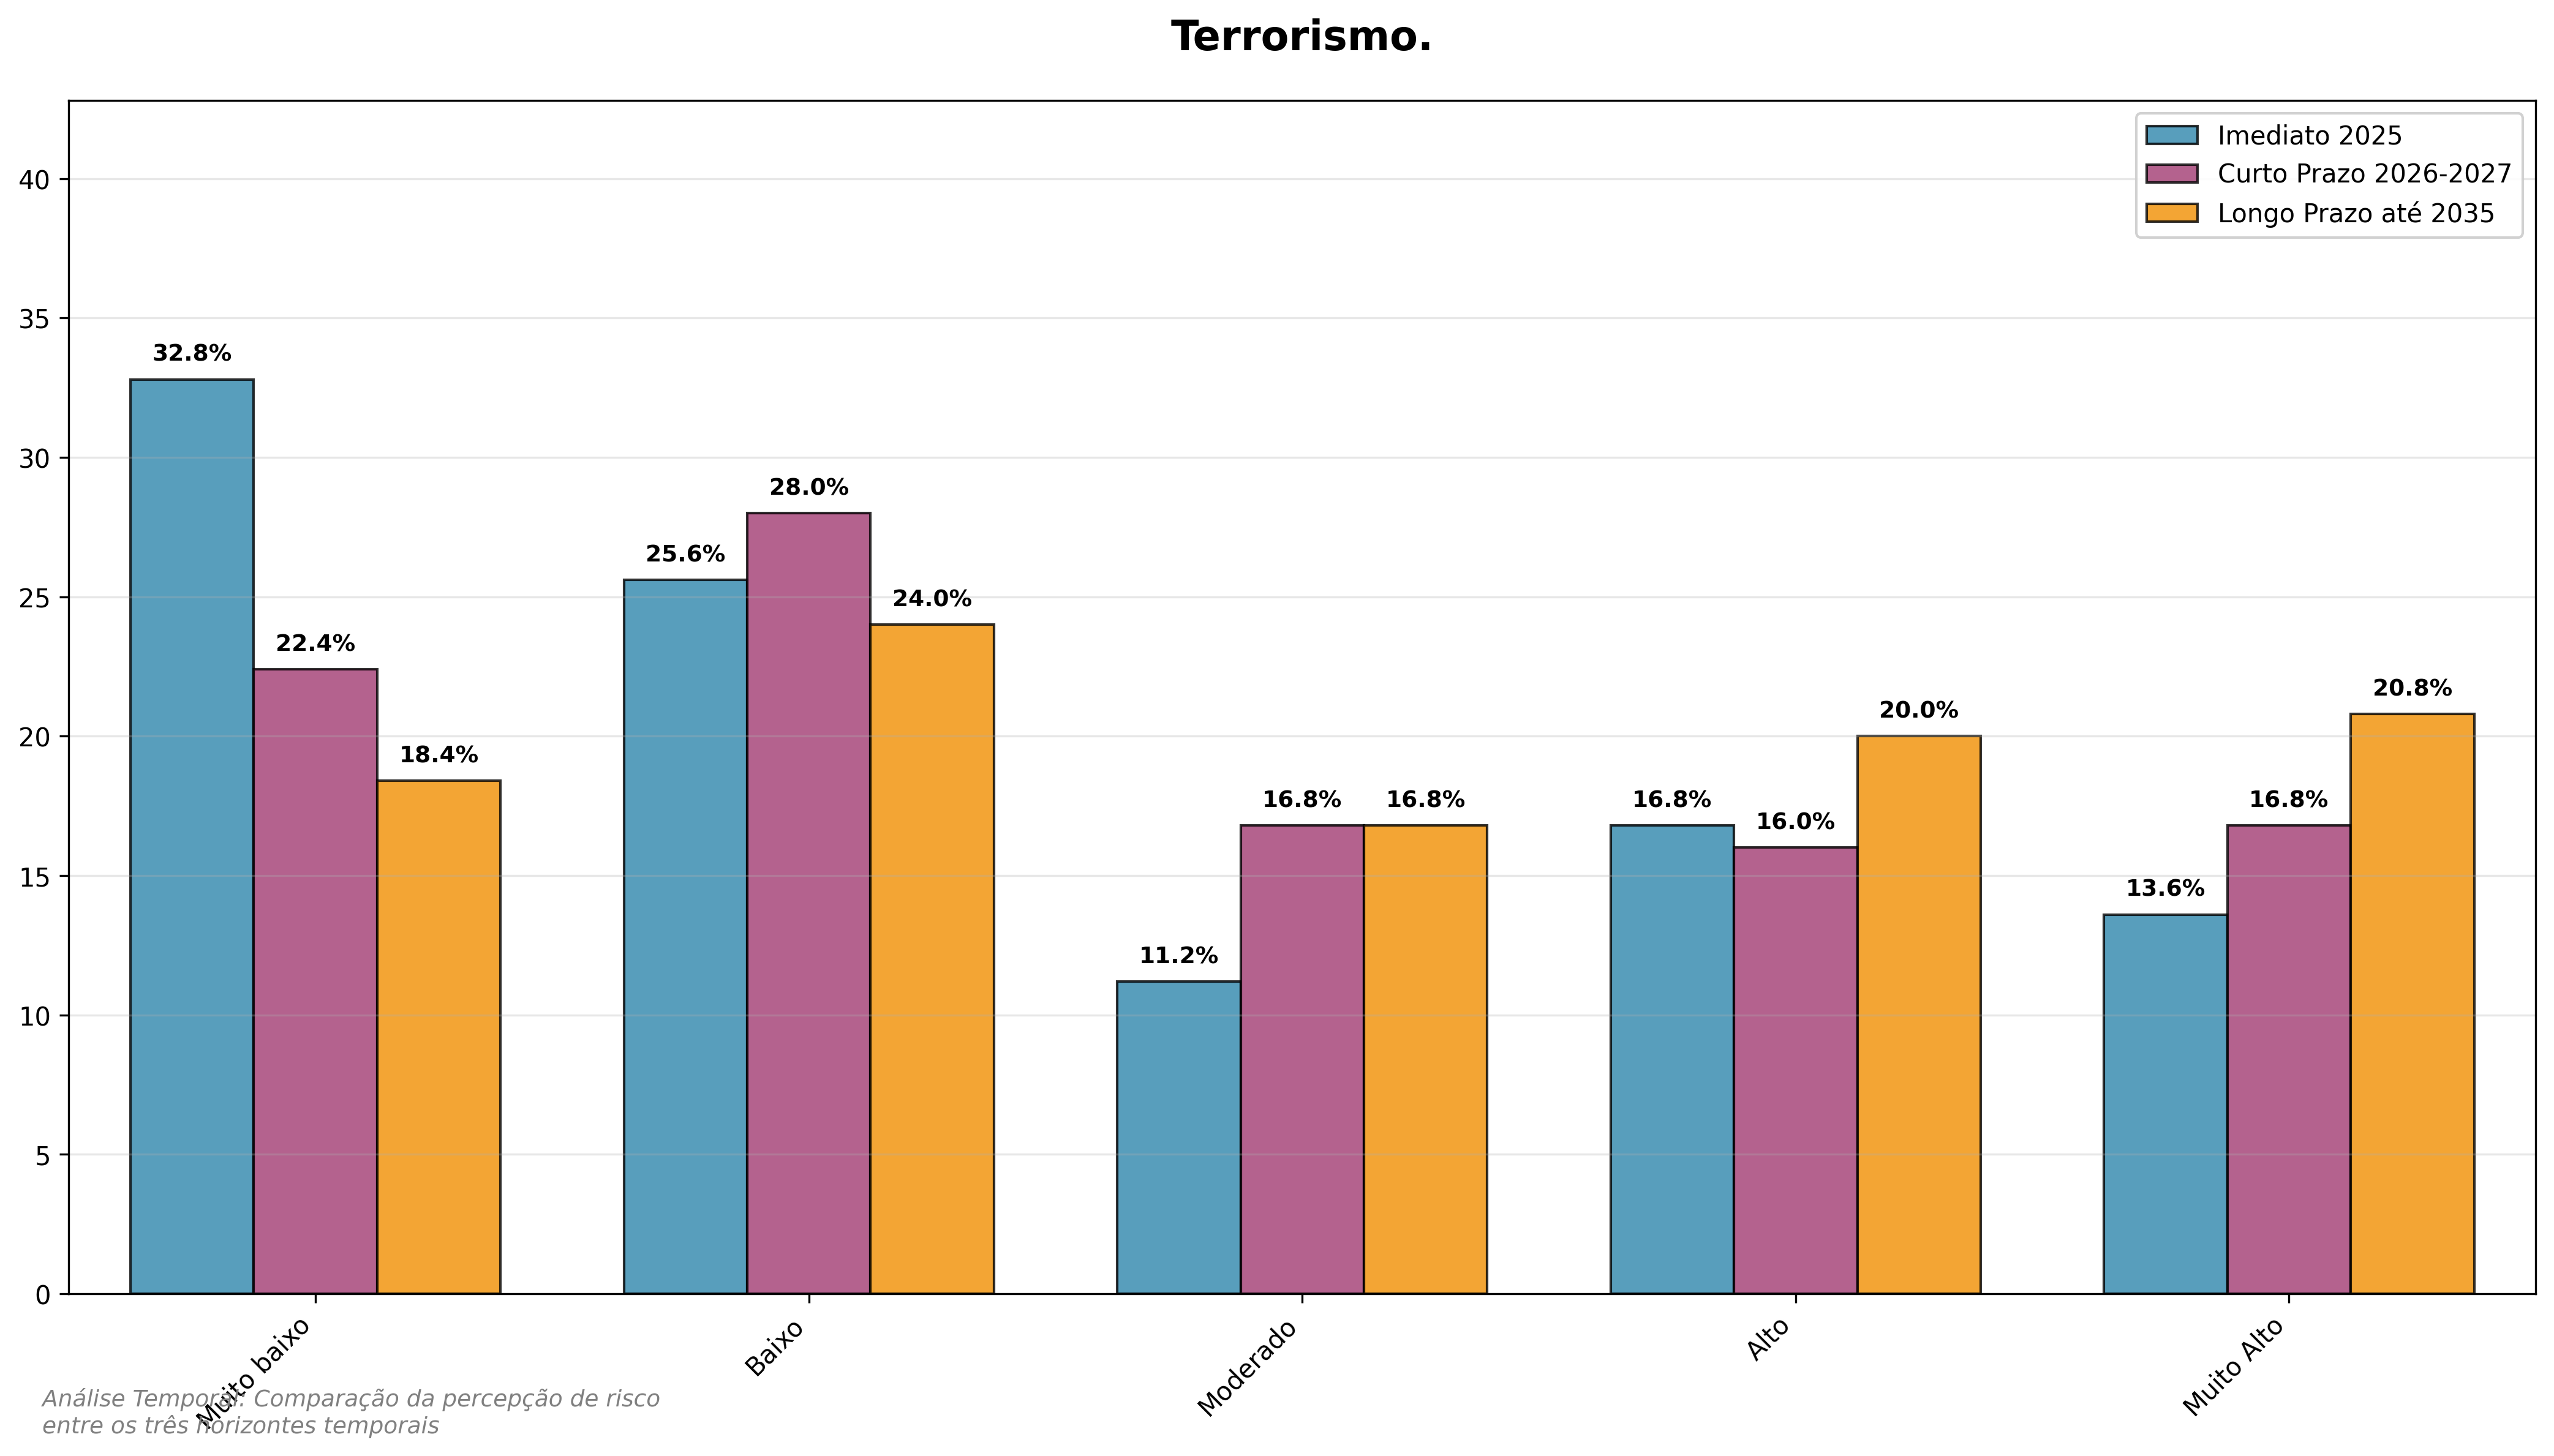
\includegraphics[keepaspectratio]{assets/geopoliticos/grafico_agrupado_3_6_temporal.png}}

\begin{tcolorbox}[enhanced jigsaw, titlerule=0mm, colback=white, title=\textcolor{quarto-callout-tip-color}{\faLightbulb}\hspace{0.5em}{Destaques}, opacityback=0, colbacktitle=quarto-callout-tip-color!10!white, leftrule=.75mm, left=2mm, colframe=quarto-callout-tip-color-frame, bottomrule=.15mm, bottomtitle=1mm, breakable, toprule=.15mm, toptitle=1mm, opacitybacktitle=0.6, arc=.35mm, coltitle=black, rightrule=.15mm]

\textbf{Imediato (2025)}: Mediana 2.0, 30\% em risco alto

\textbf{Curto Prazo (2026-2027)}: Mediana 2.0, 33\% em risco alto

\textbf{Longo Prazo (até 2035)}: Mediana 3.0, 41\% em risco alto

Devido à possibilidade de ataques terroristas a infraestruturas críticas
e áreas portuárias sensíveis, poderá ocorrer danos estruturais e
psicológicos (dos trabalhadores maritimos e portuarios) significativos,
com paralisação de operações estratégicas, o que poderá levar a custos
elevados de recuperação e reforço da segurança, impactando a resiliência
institucional e a percepção internacional de segurança dos portos
brasileiros.

\end{tcolorbox}

\subsection{Migração ou deslocamento
forçado}\label{migrauxe7uxe3o-ou-deslocamento-foruxe7ado}

O gr?fico a seguir apresenta a evolu??o temporal do risco Migração ou
deslocamento forçado.
\pandocbounded{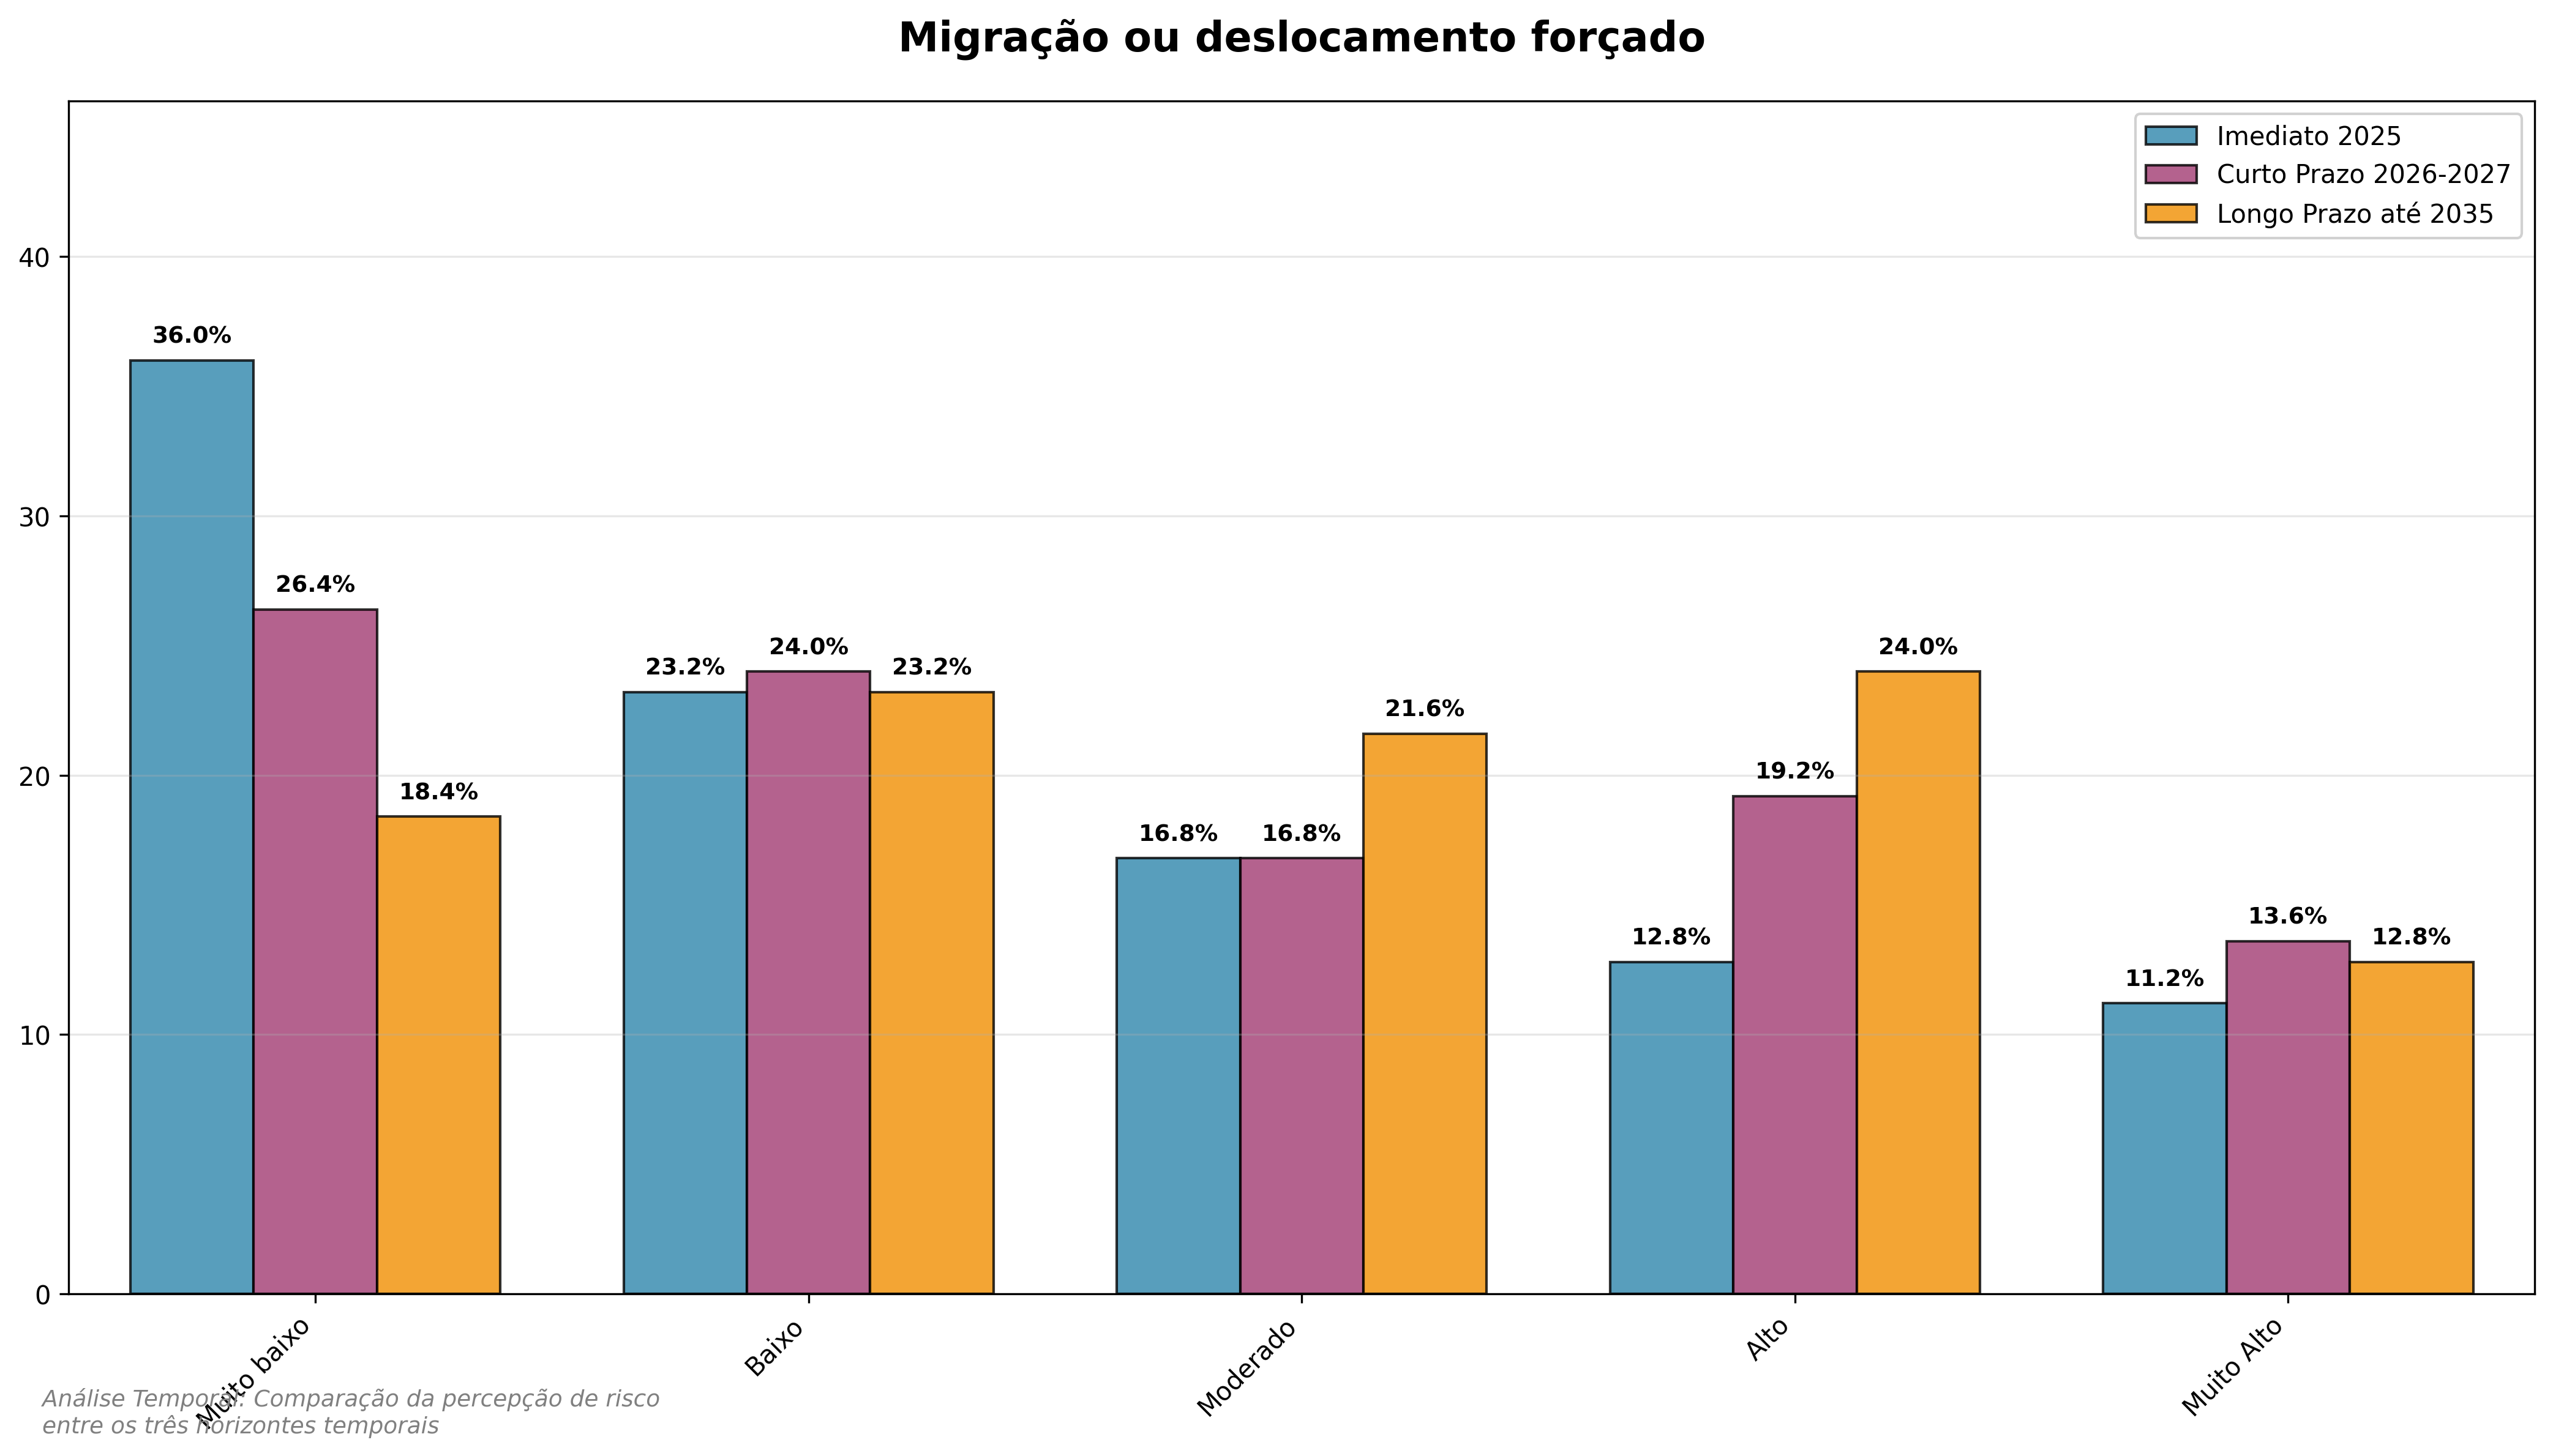
\includegraphics[keepaspectratio]{assets/geopoliticos/grafico_agrupado_3_7_temporal.png}}

\begin{tcolorbox}[enhanced jigsaw, titlerule=0mm, colback=white, title=\textcolor{quarto-callout-tip-color}{\faLightbulb}\hspace{0.5em}{Destaques}, opacityback=0, colbacktitle=quarto-callout-tip-color!10!white, leftrule=.75mm, left=2mm, colframe=quarto-callout-tip-color-frame, bottomrule=.15mm, bottomtitle=1mm, breakable, toprule=.15mm, toptitle=1mm, opacitybacktitle=0.6, arc=.35mm, coltitle=black, rightrule=.15mm]

\textbf{Imediato (2025)}: Mediana 2.0, 24\% em risco alto

\textbf{Curto Prazo (2026-2027)}: Mediana 2.0, 33\% em risco alto

\textbf{Longo Prazo (até 2035)}: Mediana 3.0, 37\% em risco alto

Devido ao aumento de fluxos migratórios forçados provocados por
conflitos, crises humanitárias ou desastres climáticos, poderá ocorrer
pressão sobre infraestruturas portuárias e demanda emergencial por
acolhimento e apoio humanitário, o que poderá levar a readequações
logísticas e uso não planejado de áreas operacionais, impactando a
função institucional dos portos como agentes de apoio à segurança e
estabilidade regional.

\end{tcolorbox}

\section{Análise Temporal
Comparativa}\label{anuxe1lise-temporal-comparativa-2}

A análise comparativa entre os horizontes temporais revela importantes
padrões:

\subsection{Tendências
Identificadas}\label{tenduxeancias-identificadas-2}

\begin{itemize}
\tightlist
\item
  \textbf{Riscos Imediatos}: Maior preocupação com conflitos
  internacionais e instabilidade política;- \textbf{Riscos de Curto
  Prazo}: Destaque para mudanças regulatórias e barreiras comerciais;-
  \textbf{Riscos de Longo Prazo}: Preocupação crescente com segurança
  portuária e crimes marítimos. \#\#\# Insights Estratégicos
\end{itemize}

\begin{enumerate}
\def\labelenumi{\arabic{enumi}.}
\tightlist
\item
  \textbf{Inteligência Estratégica}: Necessidade de monitoramento
  contínuo do cenário geopolítico global;2. \textbf{Diversificação de
  Mercados}: Reduzir dependência de regiões instáveis;3.
  \textbf{Segurança}: Fortalecer protocolos de segurança e cooperação
  internacional;4. \textbf{Resiliência Operacional}: Desenvolver
  capacidade de adaptação a mudanças regulatórias. A análise da dimensão
  geopolítica evidencia que os riscos de médio e longo prazo apresentam
  tendência de crescimento gradual, especialmente em função da
  instabilidade global e da intensificação das disputas econômicas e
  territoriais. Observa-se que riscos geoeconômicos e de natureza
  política (como sanções, conflitos regionais e volatilidade cambial)
  configuram as principais ameaças à previsibilidade e competitividade
  do setor portuário. Recomenda-se, portanto, o fortalecimento das
  capacidades institucionais de monitoramento geopolítico, o
  planejamento de contingência logística e a cooperação internacional,
  de modo a preservar a resiliência, continuidade operacional e
  relevância estratégica dos portos brasileiros em um cenário global
  cada vez mais incerto.
\end{enumerate}

\bookmarksetup{startatroot}

\chapter{Dimensão Social}\label{dimensuxe3o-social}

Este capítulo apresenta a análise dos riscos sociais com a evolução da
percepção de risco ao longo do tempo.

\section{Análise da Dimensão de Riscos Sociais no Setor
Portuário}\label{anuxe1lise-da-dimensuxe3o-de-riscos-sociais-no-setor-portuuxe1rio}

O gr?fico a seguir mostra a distribui??o dos riscos no per?odo imediato.
\pandocbounded{\includegraphics[keepaspectratio]{assets/social/grafico_barras_imediato_2025.png}}

\begin{tcolorbox}[enhanced jigsaw, titlerule=0mm, colback=white, title=\textcolor{quarto-callout-note-color}{\faInfo}\hspace{0.5em}{Destaque}, opacityback=0, colbacktitle=quarto-callout-note-color!10!white, leftrule=.75mm, left=2mm, colframe=quarto-callout-note-color-frame, bottomrule=.15mm, bottomtitle=1mm, breakable, toprule=.15mm, toptitle=1mm, opacitybacktitle=0.6, arc=.35mm, coltitle=black, rightrule=.15mm]

O gráfico apresenta o ranking dos riscos sociais no período Imediato
2025, ordenados pelo percentual de respostas em níveis altos (4-5). Os
principais destaques são:

\textbf{Riscos Mais Críticos (acima de 30\%):}

\begin{itemize}
\tightlist
\item
  \textbf{Acidentes nas operações portuárias} (30\%) - Maior risco
  social identificado;
\item
  \textbf{Insuficiência de serviços públicos essenciais} (28\%) -
  Segundo maior risco. \textbf{Riscos Elevados (25-30\%):}
\end{itemize}

- \textbf{Falhas na gestão de crises} (26\%)

- \textbf{Falhas no controle interno: fraudes ou corrupção} (26\%)

- \textbf{Ausência do Estado junto às populações próximas} (26\%)

- \textbf{Falta de recursos humanos capacitados} (27\%)

\textbf{Riscos Moderados (20-25\%):}

- \textbf{Acidentes rodoviários e ferroviários} (24\%)

- \textbf{Maior uso de tecnologias} (23\%)

- \textbf{Ocorrência de pandemias ou epidemias} (22\%)

- \textbf{Ameaças aos direitos humanos} (21\%)

\textbf{Riscos Controlados (abaixo de 20\%):}

- \textbf{Falta de participação social} (17\%)

- \textbf{Desigualdades raciais/étnicas e de gênero} (14\%)

- \textbf{Assédio moral e sexual no ambiente de trabalho} (19\%)

\textbf{Análise Geral:} A média geral de risco alto é de 23\%, indicando
um cenário de atenção moderada. Os riscos operacionais e de governança
apresentam os maiores percentuais, enquanto questões relacionadas a
diversidade e participação social mostram menores níveis de preocupação
neste período.

\end{tcolorbox}

\section{Análise Temporal da Dimensão
Social}\label{anuxe1lise-temporal-da-dimensuxe3o-social}

O gr?fico a seguir sintetiza a evolu??o temporal das vari?veis da
dimens?o social.
\pandocbounded{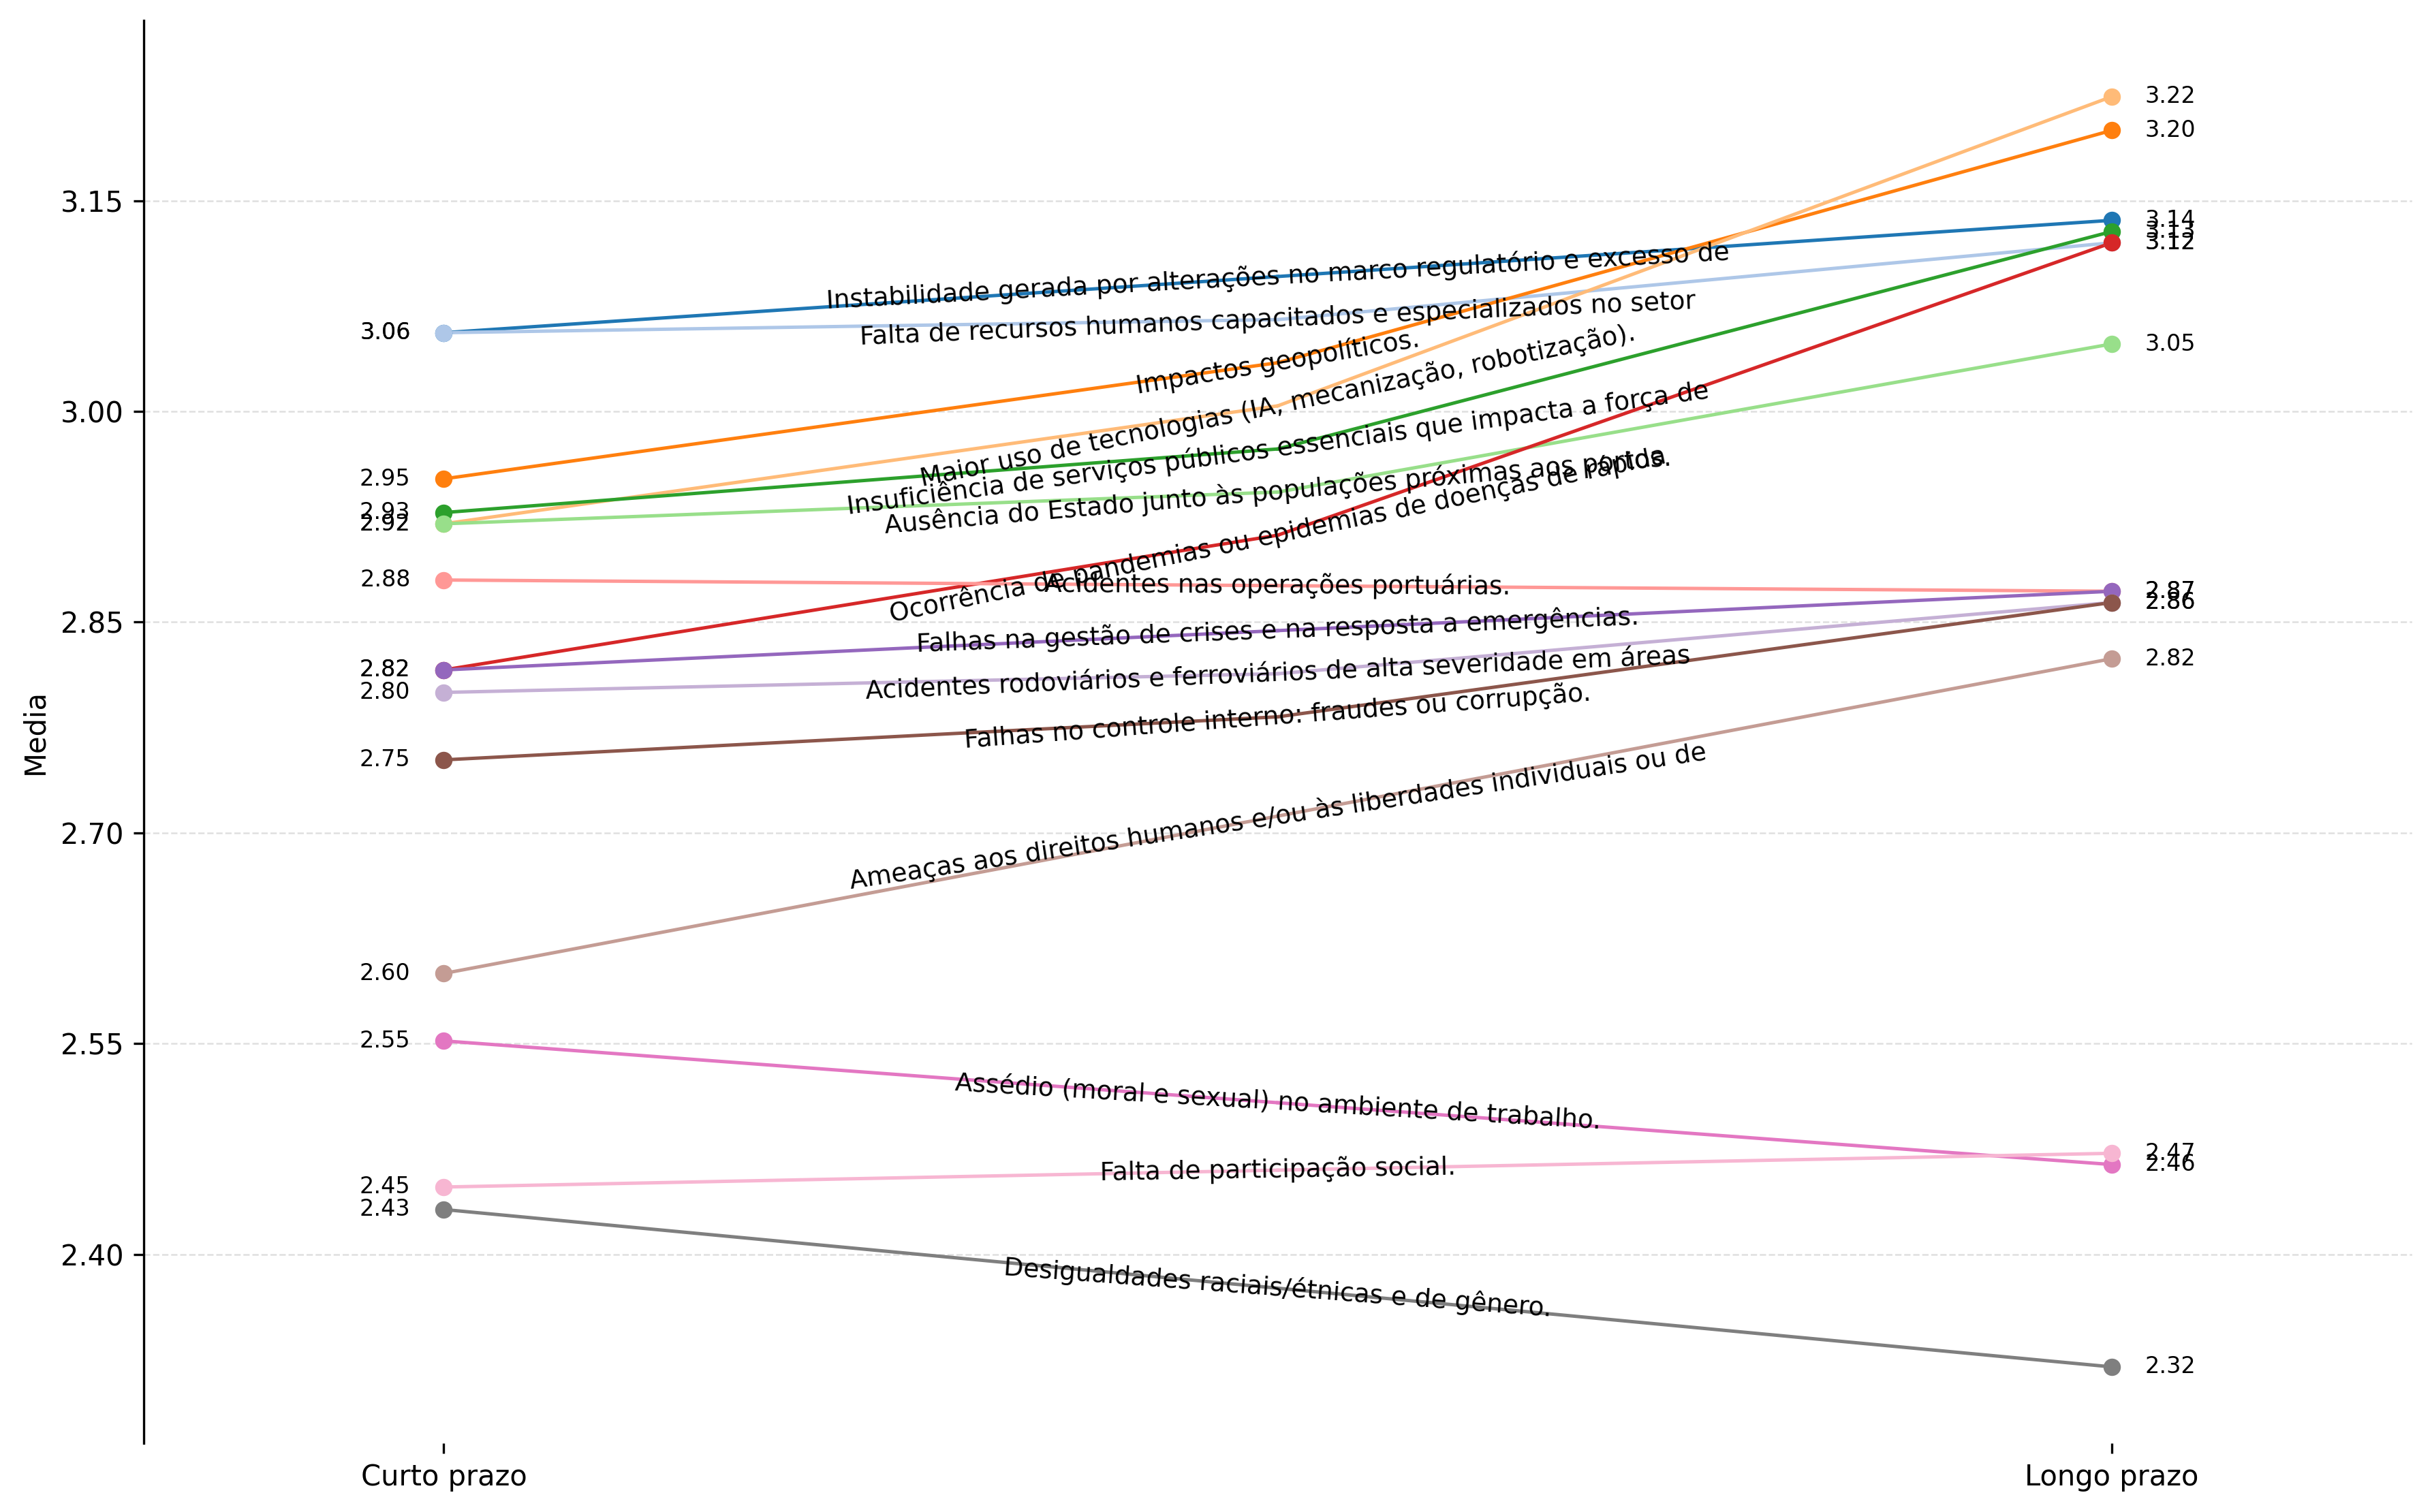
\includegraphics[keepaspectratio]{assets/slopegraphs_por_dimensao/slopegraph_social.png}}

A dimensão social compreende variáveis críticas, abrangendo desde
direitos humanos até questões trabalhistas e participação comunitária. O
slopegraph social revela como as percepções sobre impacto social
evoluem, indicando áreas que demandam atenção contínua.

\subsection{Insights da Análise Temporal
Social}\label{insights-da-anuxe1lise-temporal-social}

A análise temporal dos riscos sociais revela padrões importantes na
evolução das percepções entre o curto prazo (2026-2027) e o longo prazo
(até 2035):

\subsubsection{Principais Tendências
Identificadas}\label{principais-tenduxeancias-identificadas}

\begin{itemize}
\item
  \textbf{Crescimento Tecnológico}: O risco associado ao maior uso de
  tecnologias (IA, mecanização, robotização) apresenta o maior
  crescimento (+103\%), passando de 23\% para 47\% de percepção de risco
  alto;- \textbf{Preocupação Sanitária}: Pandemias e epidemias mostram
  aumento significativo (+74\%), refletindo as lições aprendidas
  pós-COVID;- \textbf{Direitos Humanos}: Ameaças aos direitos humanos
  apresentam crescimento moderado (+58\%), indicando deterioração
  gradual;- \textbf{Serviços Essenciais}: Insuficiência de serviços
  públicos mantém-se como risco crítico e persistente em todos os
  períodos. \#\#\#\# Riscos Crônicos vs Emergentes
\item
  \textbf{Riscos Crônicos}: Acidentes operacionais, falhas na gestão de
  crises e corrupção mantêm-se elevados e persistentes;- \textbf{Riscos
  Emergentes}: Transformação digital e questões sanitárias mostram maior
  crescimento temporal;- \textbf{Riscos Controlados}: Desigualdades,
  participação social e assédio mantêm-se em níveis controlados, embora
  com crescimento moderado. \#\#\#\# Implicações Estratégicas para a
  Dimensão Social
\end{itemize}

A análise temporal social indica necessidade de:

\begin{enumerate}
\def\labelenumi{\arabic{enumi}.}
\tightlist
\item
  \textbf{Investimentos em Capacitação Digital}: Preparar a força de
  trabalho para transformação tecnológica;
\item
  \textbf{Resiliência Sanitária}: Fortalecer protocolos de saúde e
  segurança pós-pandemia;
\item
  \textbf{Serviços Essenciais}: Desenvolver parcerias para garantir
  serviços básicos às comunidades;
\item
  \textbf{Direitos Humanos}: Implementar mecanismos robustos de proteção
  e salvaguarda. \#\# Análise Temporal dos Riscos Sociais
\end{enumerate}

\begin{tcolorbox}[enhanced jigsaw, titlerule=0mm, colback=white, title=\textcolor{quarto-callout-tip-color}{\faLightbulb}\hspace{0.5em}{Visualização Temporal}, opacityback=0, colbacktitle=quarto-callout-tip-color!10!white, leftrule=.75mm, left=2mm, colframe=quarto-callout-tip-color-frame, bottomrule=.15mm, bottomtitle=1mm, breakable, toprule=.15mm, toptitle=1mm, opacitybacktitle=0.6, arc=.35mm, coltitle=black, rightrule=.15mm]

Esta seção apresenta a análise dos três horizontes temporais para a
dimensão social, facilitando a comparação da evolução da percepção de
risco ao longo do tempo. Cada gráfico mostra a distribuição percentual
das respostas por nível de risco nos períodos Imediato 2025, Curto Prazo
2026-2027 e Longo Prazo até 2035.

\end{tcolorbox}

\subsection{Ameaças aos direitos humanos e/ou às liberdades individuais
ou de
grupo}\label{ameauxe7as-aos-direitos-humanos-eou-uxe0s-liberdades-individuais-ou-de-grupo}

O gr?fico a seguir apresenta a evolu??o temporal do risco Ameaças aos
direitos humanos e/ou às liberdades individuais ou de grupo.
\pandocbounded{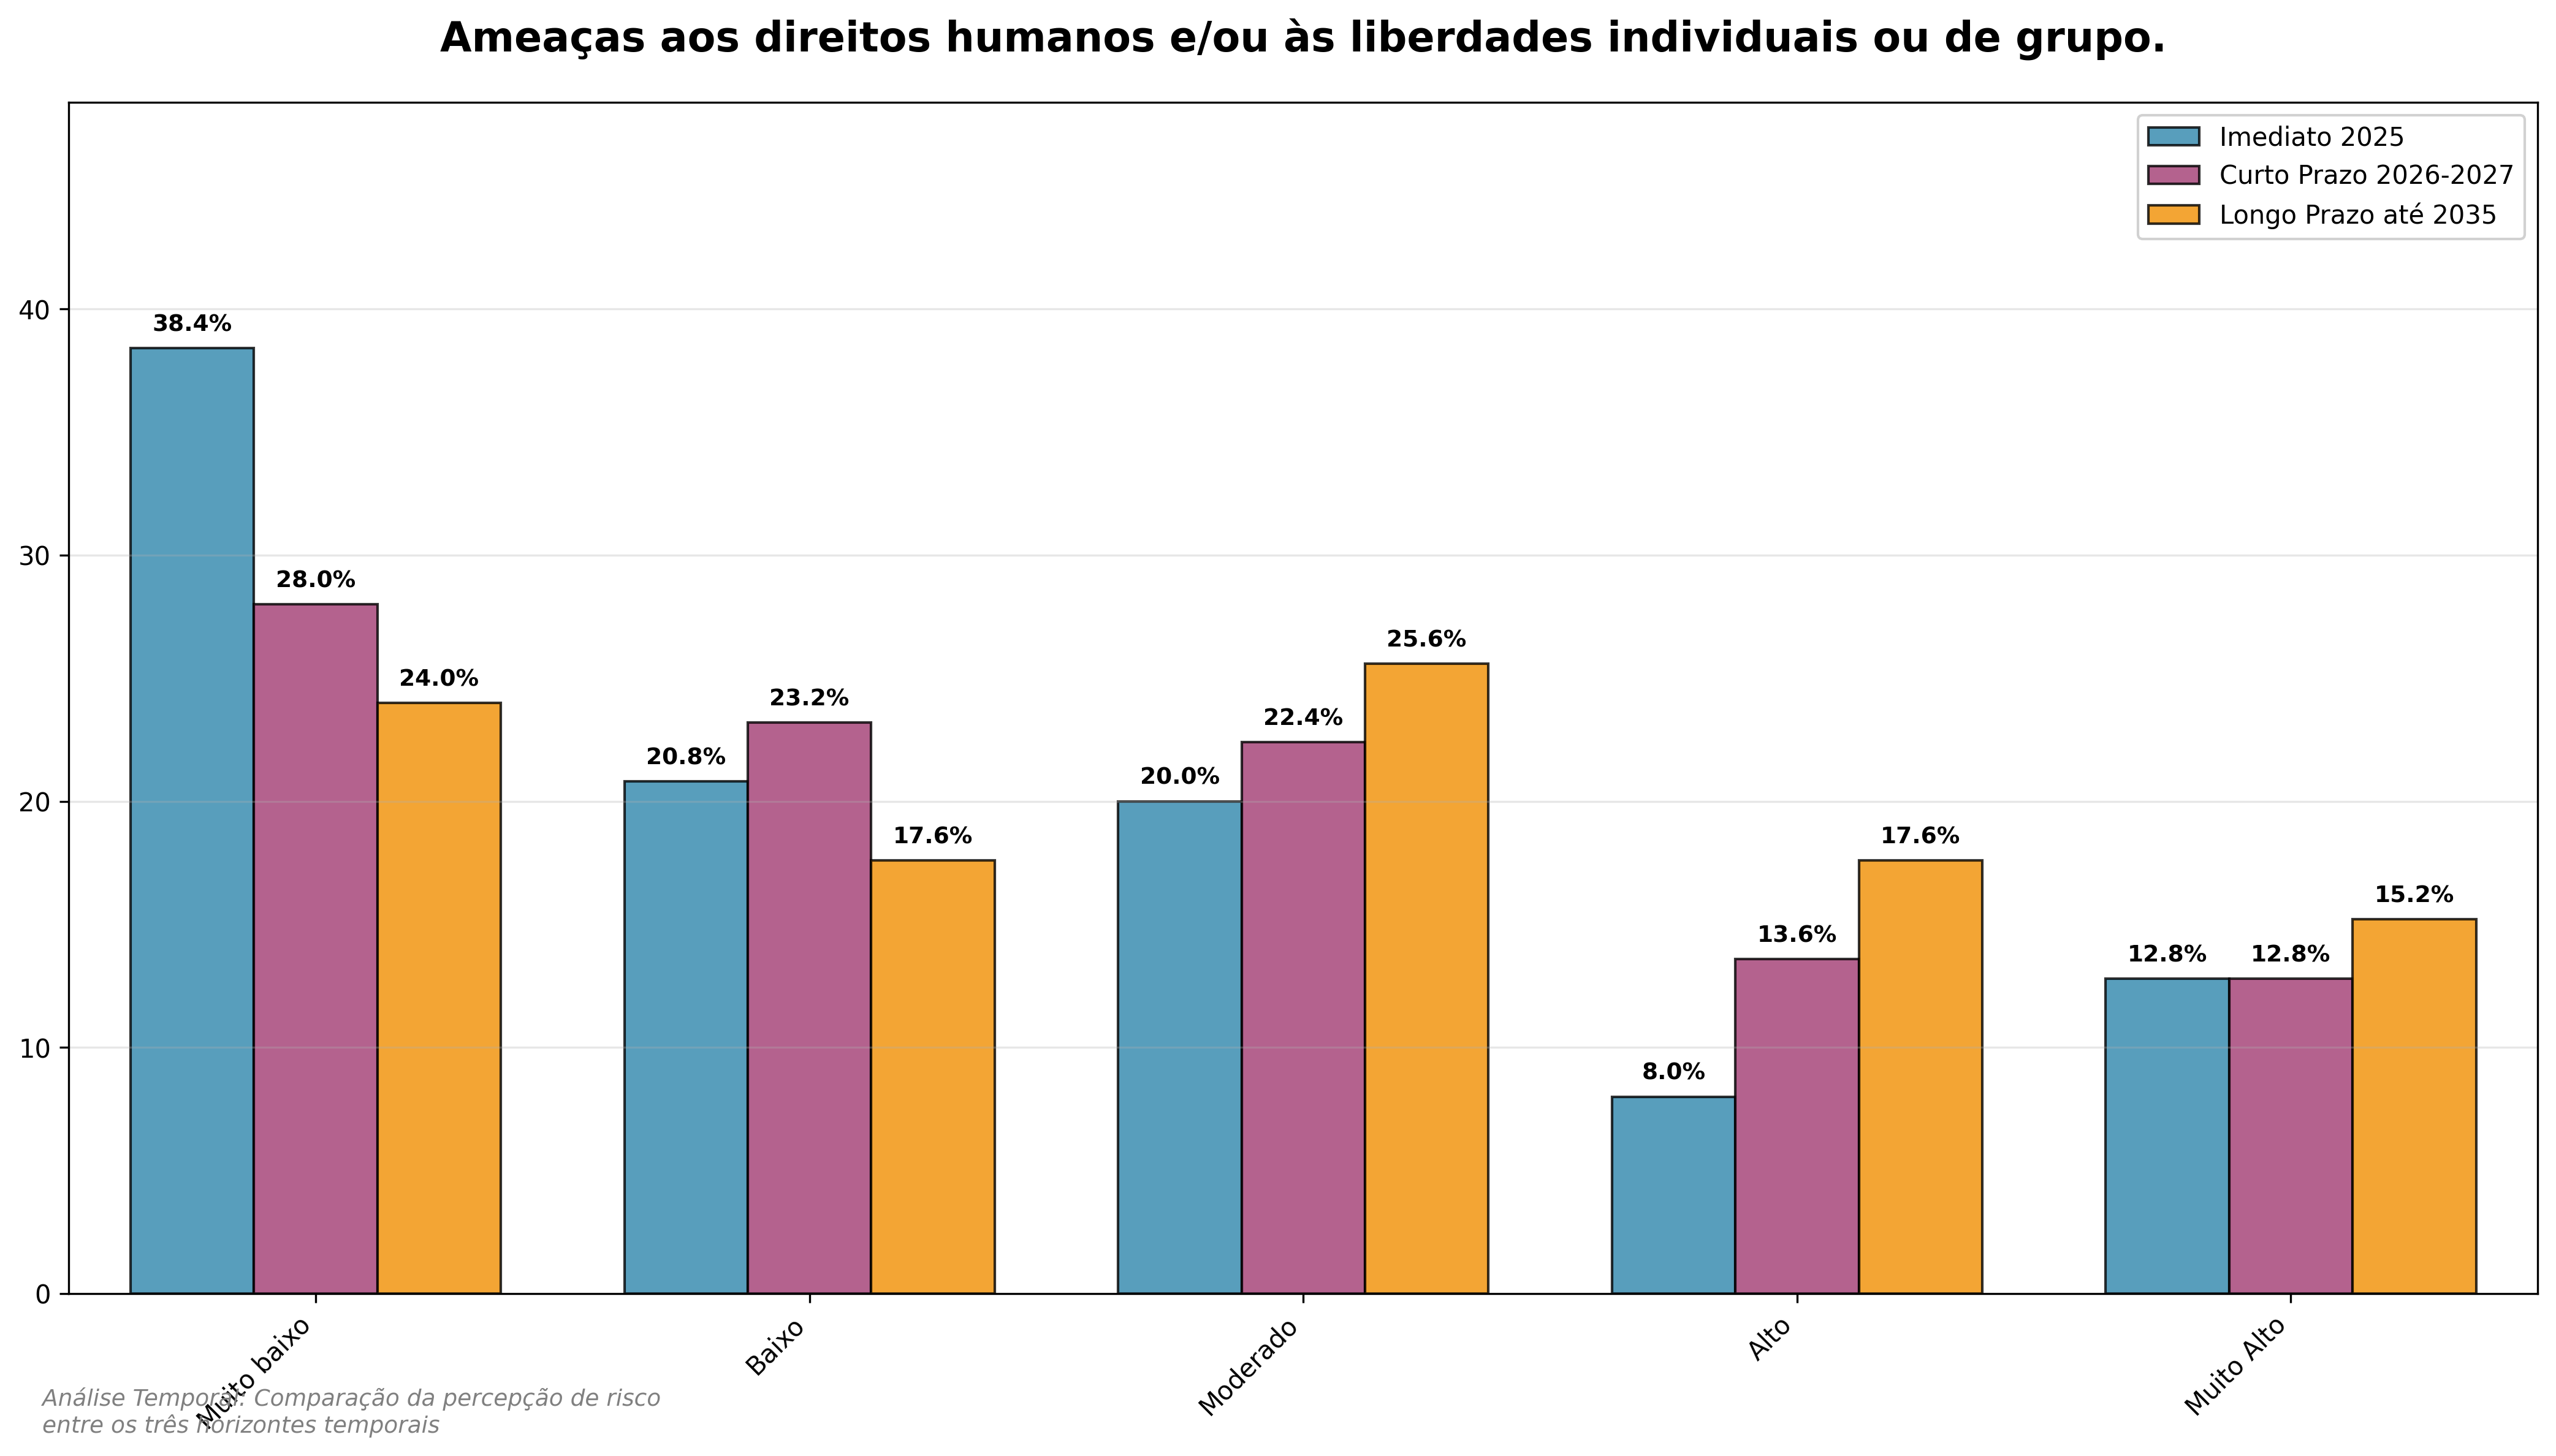
\includegraphics[keepaspectratio]{assets/social/grafico_agrupado_4_1_temporal.png}}

\begin{tcolorbox}[enhanced jigsaw, titlerule=0mm, colback=white, title=\textcolor{quarto-callout-note-color}{\faInfo}\hspace{0.5em}{Destaque}, opacityback=0, colbacktitle=quarto-callout-note-color!10!white, leftrule=.75mm, left=2mm, colframe=quarto-callout-note-color-frame, bottomrule=.15mm, bottomtitle=1mm, breakable, toprule=.15mm, toptitle=1mm, opacitybacktitle=0.6, arc=.35mm, coltitle=black, rightrule=.15mm]

\textbf{Evolução da Percepção de Risco:} - \textbf{Tendência de
crescimento}: Aumento progressivo da percepção de risco ao longo do
tempo - \textbf{Mediana}: Evolui de 2.0 (2025) para 3.0 (2035),
indicando piora da situação

- \textbf{Risco Alto (níveis 4-5)}: Cresce de 21\% (2025) para 33\%
(2035) - aumento de 58\%

- \textbf{Risco Baixo (níveis 1-2)}: Redução de 58\% (2025) para 40\%
(2035)

\textbf{Contexto Detalhado por Período:}

\textbf{Período Imediato 2025:} Devido às ameaças aos direitos humanos e
às liberdades individuais ou de grupo, poderá acontecer o aumento de
denúncias, pressão internacional e litígios coletivos por violações, o
que poderá levar a sanções administrativas, desgastes reputacionais e
necessidade de reparar danos impactando a integridade institucional e o
compromisso com direitos humanos. No período imediato 2025, 21\% das
respostas permanecem nos níveis 4-5 e a mediana em 2 indica um nível
controlado sob vigilância.

\textbf{Período Curto Prazo 2026-2027:} A mesma dinâmica de ameaças aos
direitos humanos evolui para um nível emergente que merece
acompanhamento próximo, com 26\% das respostas nos níveis 4-5 e mediana
em 2, indicando transição para risco moderado.

\textbf{Período Longo Prazo até 2035:} A situação se agrava
significativamente, atingindo 33\% de respostas nos níveis 4-5 com
mediana em 3, configurando um nível elevado que demanda planos de ação
priorizados.

\textbf{Implicações Estratégicas:} A tendência de deterioração sugere
necessidade de planejamento estratégico robusto para proteção de
direitos humanos no longo prazo, com investimentos crescentes em
compliance e mecanismos de salvaguarda. A evolução de controlado para
crítico indica urgência de medidas preventivas e corretivas escalonadas
ao longo do tempo.

\end{tcolorbox}

\subsection{Ocorrência de pandemias ou epidemias de doenças de rápida
disseminação}\label{ocorruxeancia-de-pandemias-ou-epidemias-de-doenuxe7as-de-ruxe1pida-disseminauxe7uxe3o}

O gr?fico a seguir apresenta a evolu??o temporal do risco Ocorrência de
pandemias ou epidemias de doenças de rápida disseminação.
\pandocbounded{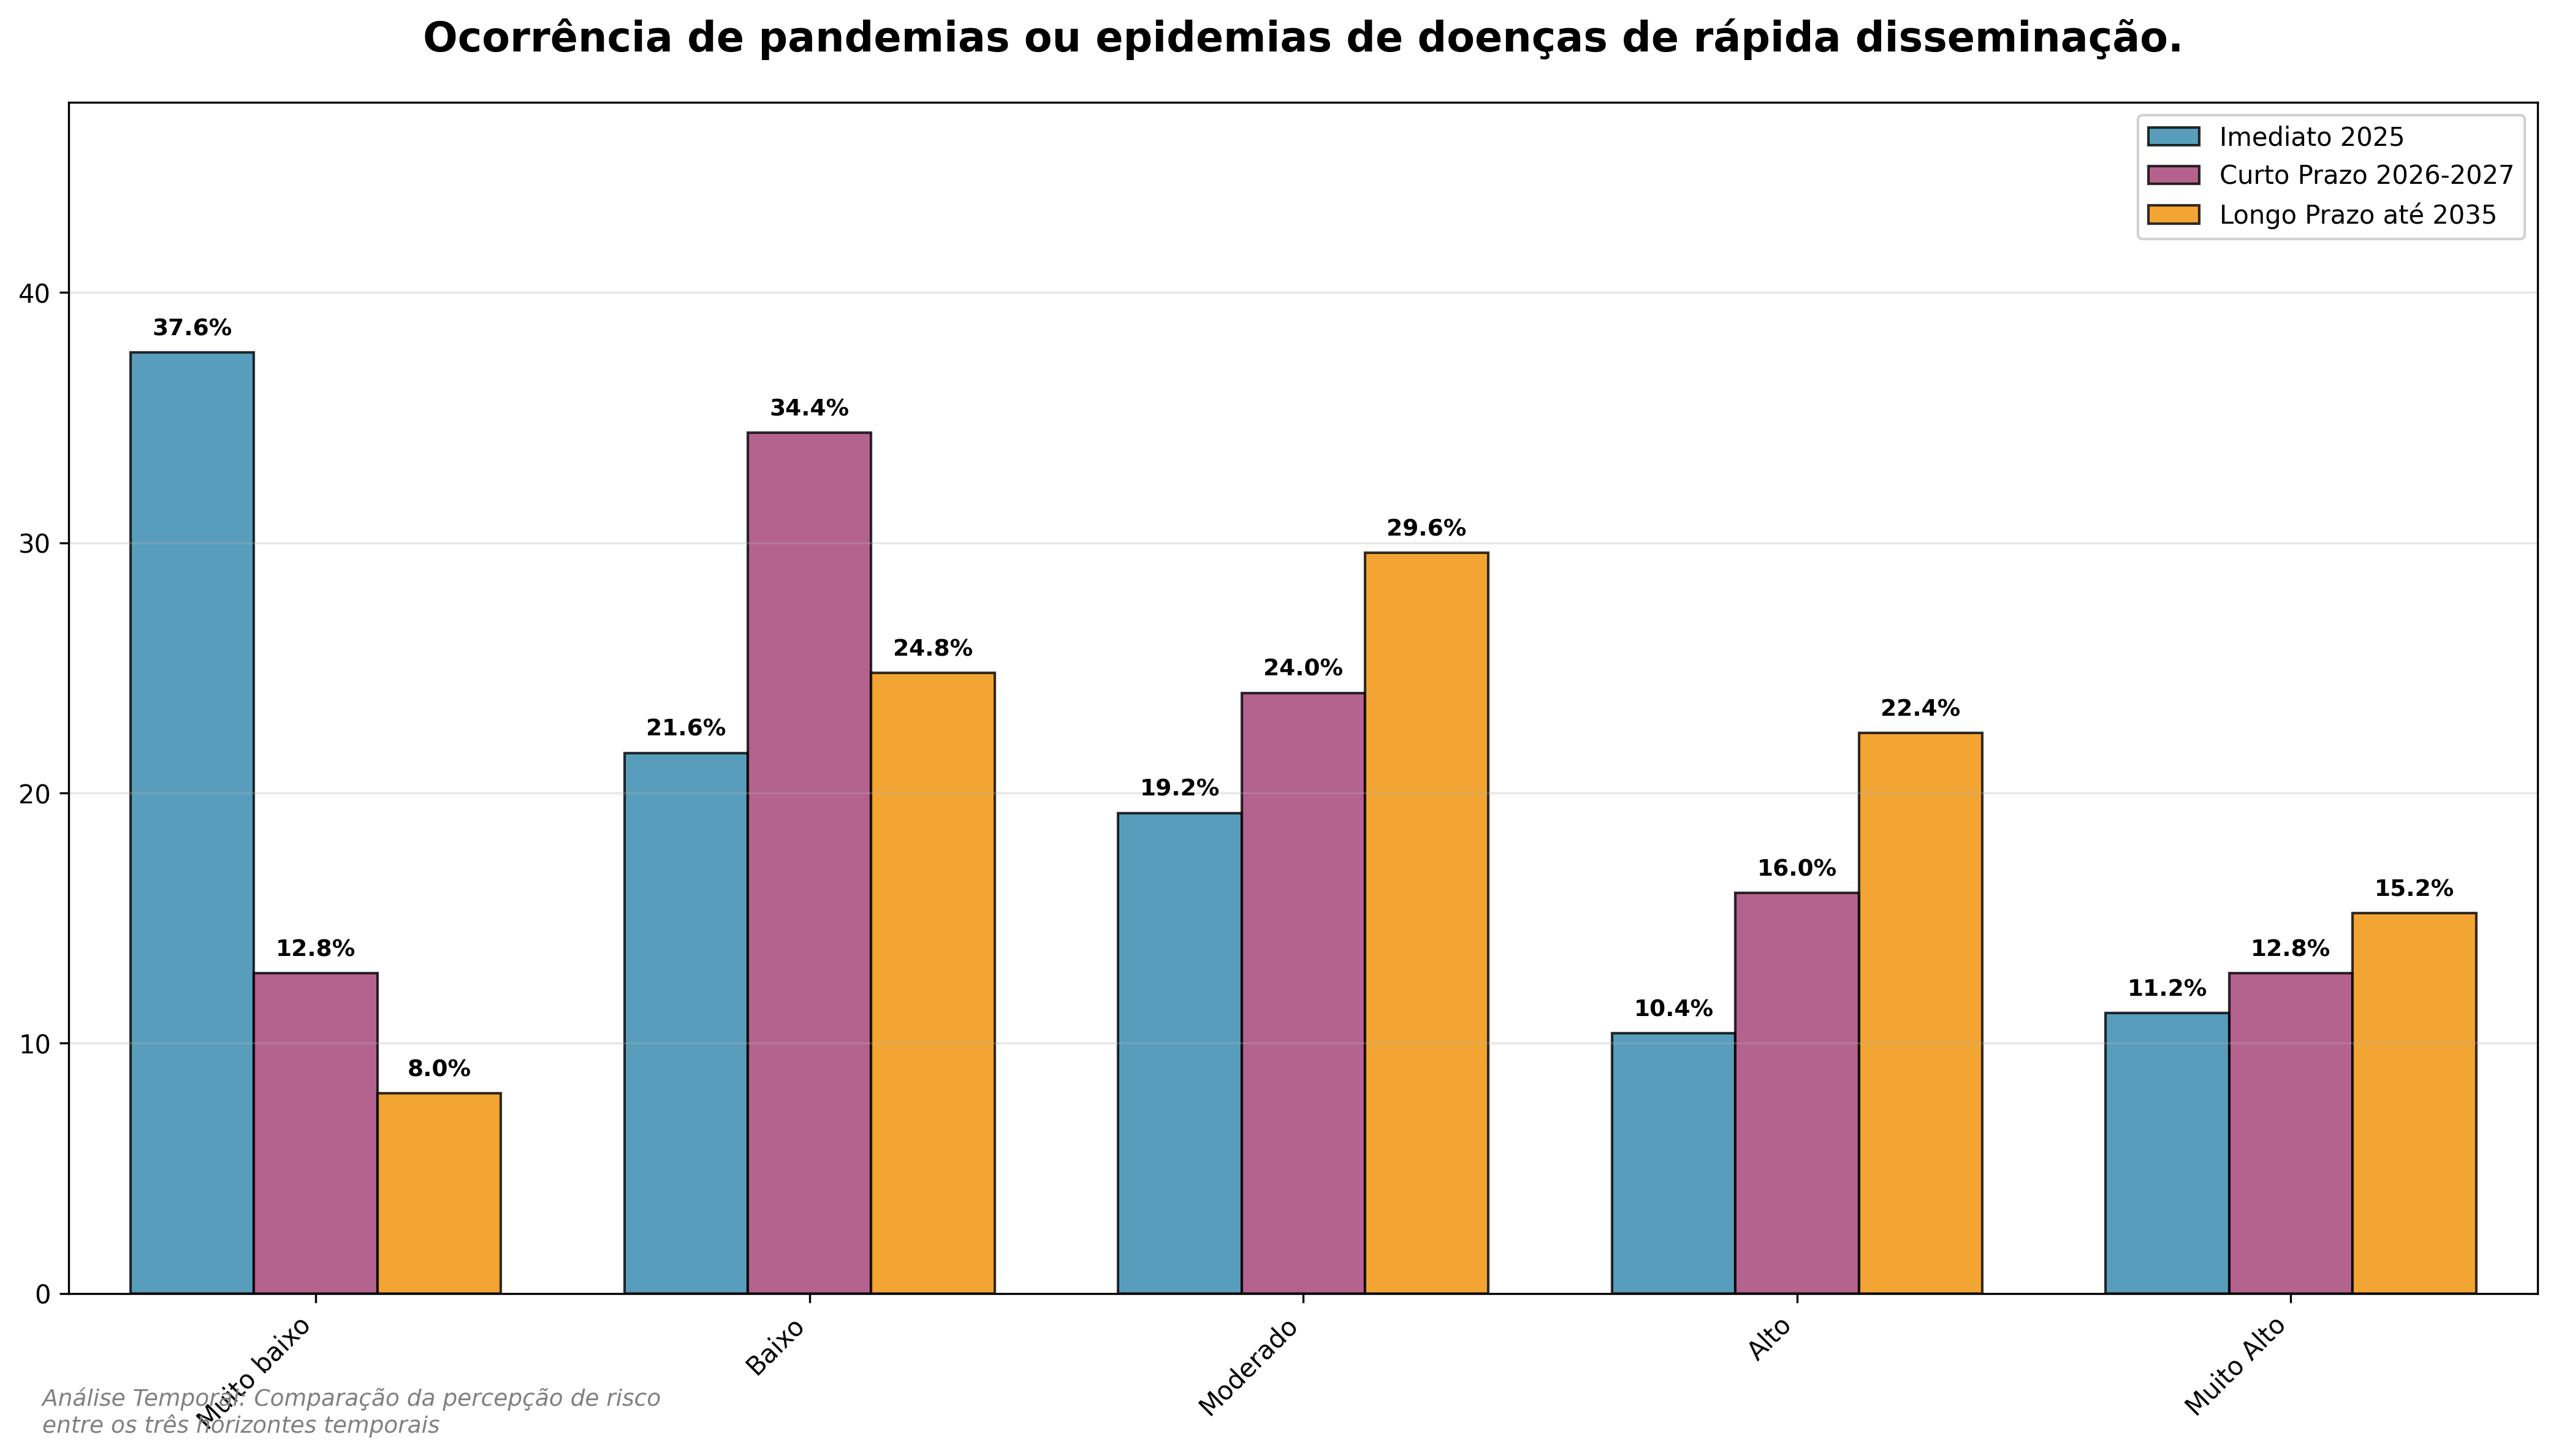
\includegraphics[keepaspectratio]{assets/social/grafico_agrupado_4_2_temporal.png}}

\begin{tcolorbox}[enhanced jigsaw, titlerule=0mm, colback=white, title=\textcolor{quarto-callout-note-color}{\faInfo}\hspace{0.5em}{Destaque}, opacityback=0, colbacktitle=quarto-callout-note-color!10!white, leftrule=.75mm, left=2mm, colframe=quarto-callout-note-color-frame, bottomrule=.15mm, bottomtitle=1mm, breakable, toprule=.15mm, toptitle=1mm, opacitybacktitle=0.6, arc=.35mm, coltitle=black, rightrule=.15mm]

\textbf{Evolução da Percepção de Risco:}

- \textbf{Tendência de crescimento acelerado}: Aumento significativo da
preocupação com saúde pública - \textbf{Mediana}: Evolui de 2.0 (2025)
para 3.0 (2035)

- \textbf{Risco Alto (níveis 4-5)}: Cresce de 22\% (2025) para 38\%
(2035) - aumento de 74\%

- \textbf{Risco Baixo (níveis 1-2)}: Redução de 57\% (2025) para 33\%
(2035)

\textbf{Contexto Detalhado por Período:}

\textbf{Período Imediato 2025:} Devido à ocorrência de pandemias ou
epidemias de doenças de rápida disseminação, poderá acontecer novos
surtos que provoquem ausências em massa e protocolos sanitários
emergenciais, o que poderá levar a paralisações operacionais, atrasos
logísticos e custos extraordinários de proteção impactando a
continuidade dos serviços portuários e a saúde da força de trabalho. No
período imediato 2025, 22\% das respostas permanecem nos níveis 4-5 e a
mediana em 2 indica um nível controlado sob vigilância.

\textbf{Período Curto Prazo 2026-2027:} A preocupação com pandemias
evolui para um nível moderado com tendência de crescimento, atingindo
29\% das respostas nos níveis 4-5 com mediana em 3, indicando transição
para risco elevado.

\textbf{Período Longo Prazo até 2035:} A situação se torna crítica, com
38\% das respostas nos níveis 4-5 e mediana em 3, configurando um nível
elevado que demanda planos de ação priorizados.

\textbf{Implicações Estratégicas:} A crescente preocupação com pandemias
indica necessidade de fortalecimento permanente de protocolos sanitários
e planos de contingência para garantir resiliência operacional. A
evolução de controlado para crítico reflete as lições aprendidas
pós-COVID e a percepção de maior vulnerabilidade a eventos sanitários
globais.

\end{tcolorbox}

\subsection{Insuficiência de serviços públicos essenciais que impacta a
força de trabalho vinculada ao setor
portuário}\label{insuficiuxeancia-de-serviuxe7os-puxfablicos-essenciais-que-impacta-a-foruxe7a-de-trabalho-vinculada-ao-setor-portuuxe1rio}

O gr?fico a seguir apresenta a evolu??o temporal do risco Insuficiência
de serviços públicos essenciais que impacta a força de trabalho
vinculada ao setor portuário.
\pandocbounded{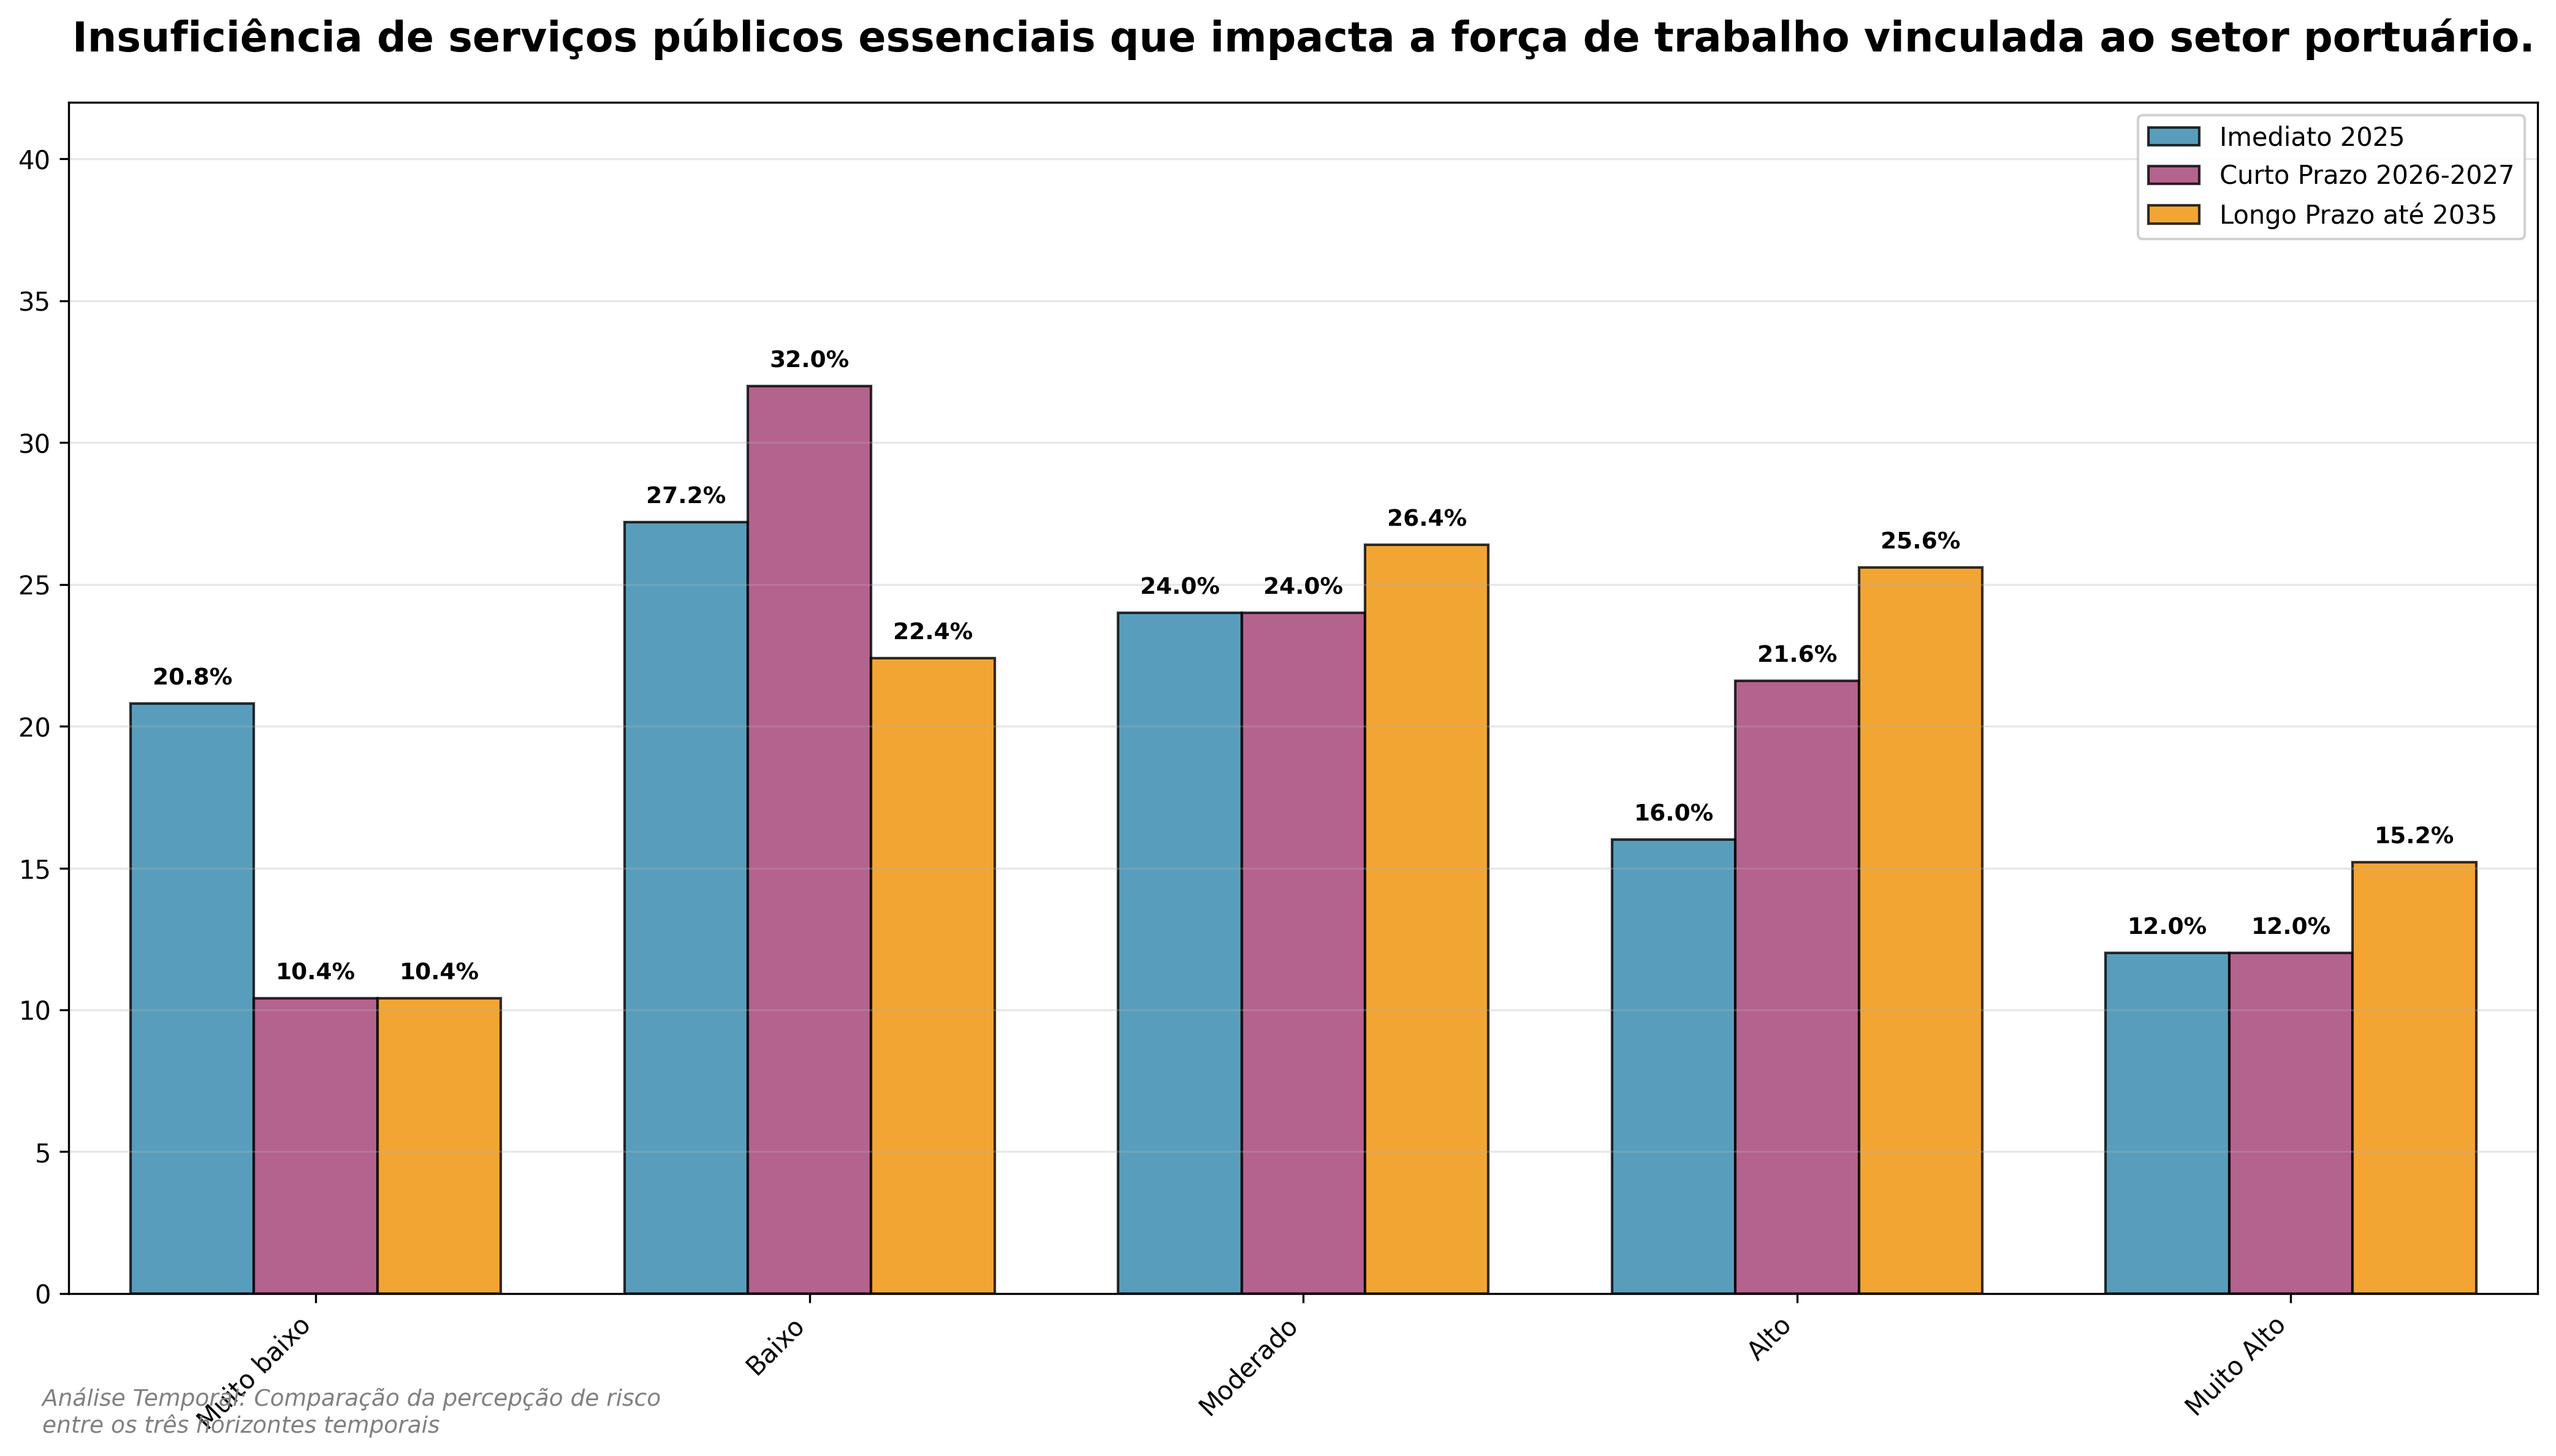
\includegraphics[keepaspectratio]{assets/social/grafico_agrupado_4_3_temporal.png}}

\begin{tcolorbox}[enhanced jigsaw, titlerule=0mm, colback=white, title=\textcolor{quarto-callout-note-color}{\faInfo}\hspace{0.5em}{Destaque}, opacityback=0, colbacktitle=quarto-callout-note-color!10!white, leftrule=.75mm, left=2mm, colframe=quarto-callout-note-color-frame, bottomrule=.15mm, bottomtitle=1mm, breakable, toprule=.15mm, toptitle=1mm, opacitybacktitle=0.6, arc=.35mm, coltitle=black, rightrule=.15mm]

\textbf{Evolução da Percepção de Risco:}

- \textbf{Tendência de deterioração crítica}: Piora consistente ao longo
do tempo

- \textbf{Mediana}: Mantém-se em 3.0 em todos os períodos, indicando
persistência do problema

- \textbf{Risco Alto (níveis 4-5)}: Cresce de 28\% (2025) para 41\%
(2035) - aumento de 46\%

- \textbf{Risco Baixo (níveis 1-2)}: Redução de 36\% (2025) para 24\%
(2035)

\textbf{Contexto Detalhado por Período:}

\textbf{Período Imediato 2025:} Devido à insuficiência de serviços
públicos essenciais nas áreas adjacentes, poderá acontecer falhas
persistentes em saneamento, saúde, transporte e segurança para
trabalhadores e comunidades, o que poderá levar a aumento de
vulnerabilidades sociais, absenteísmo e protestos comunitários
impactando a estabilidade operacional e as relações com as comunidades
do entorno. No período imediato 2025, 28\% das respostas permanecem nos
níveis 4-5 e a mediana em 3 indica um nível moderado com tendência de
crescimento.

\textbf{Período Curto Prazo 2026-2027:} A situação evolui para um nível
elevado, atingindo 34\% das respostas nos níveis 4-5 com mediana em 3,
configurando um patamar crítico que demanda planos de ação priorizados.

\textbf{Período Longo Prazo até 2035:} A insuficiência de serviços
essenciais se torna crítica, com 41\% das respostas nos níveis 4-5 e
mediana em 3, indicando um patamar crítico que requer medidas imediatas.

\textbf{Implicações Estratégicas:} A insuficiência de serviços
essenciais representa um risco crônico que exige parcerias
público-privadas e investimentos estruturais para garantir
sustentabilidade operacional. A persistência do problema em todos os
períodos indica necessidade de soluções sistêmicas e colaborativas entre
setor portuário e poder público.

\end{tcolorbox}

\subsection{Impactos geopolíticos}\label{impactos-geopoluxedticos}

O gr?fico a seguir apresenta a evolu??o temporal do risco Impactos
geopolíticos.
\pandocbounded{
\includegraphics[keepaspectratio]{assets/social/grafico_agrupado_4_4_temporal.png}}

\begin{tcolorbox}[enhanced jigsaw, titlerule=0mm, colback=white, title=\textcolor{quarto-callout-note-color}{\faInfo}\hspace{0.5em}{Destaque}, opacityback=0, colbacktitle=quarto-callout-note-color!10!white, leftrule=.75mm, left=2mm, colframe=quarto-callout-note-color-frame, bottomrule=.15mm, bottomtitle=1mm, breakable, toprule=.15mm, toptitle=1mm, opacitybacktitle=0.6, arc=.35mm, coltitle=black, rightrule=.15mm]

\textbf{Evolução da Percepção de Risco:}

\begin{itemize}
\tightlist
\item
  \textbf{Tendência de escalada}: risco alto sobe de 28\% (2025) para
  48\% (2035);- \textbf{Mediana}: avança de 2,0 para 3,0, indicando
  transição para patamar estrutural;- \textbf{Risco baixo (níveis 1-2)}:
  recua de 52\% para 32\%, mostrando perda acelerada de confiança.
  \textbf{Contexto Detalhado por Período:}
\end{itemize}

\textbf{Período Imediato 2025:} Mesmo com mediana 2, quase um terço dos
respondentes já associa conflitos e tensões globais a interrupções
logísticas, com 28\% em níveis altos e 52\% ainda confiando em
estabilidade de curto prazo.

\textbf{Período Curto Prazo 2026-2027:} A mediana passa para 3 e o risco
alto chega a 38\%, refletindo impactos de mudanças nas cadeias de
suprimentos, flutuações cambiais e barreiras comerciais emergentes.

\textbf{Período Longo Prazo até 2035:} O risco se consolida como
prioritário: 48\% nos níveis 4-5 e apenas 32\% em risco baixo,
traduzindo expectativa de cenário geopolítico mais volátil e
imprevisível.

\textbf{Implicações Estratégicas:} O setor portuário precisa fortalecer
inteligência estratégica, contratos flexíveis e redes de fornecedores em
múltiplas geografias para absorver choques geopolíticos. Aumento da
cooperação internacional, protocolos de segurança integrada e planos de
contingência logística são fundamentais para preservar competitividade e
continuidade operacional.

\end{tcolorbox}

\subsection{Acidentes rodoviários e ferroviários de alta severidade em
áreas próximas aos
portos}\label{acidentes-rodoviuxe1rios-e-ferroviuxe1rios-de-alta-severidade-em-uxe1reas-pruxf3ximas-aos-portos}

O gr?fico a seguir apresenta a evolu??o temporal do risco Acidentes
rodoviários e ferroviários de alta severidade em áreas próximas aos
portos.
\pandocbounded{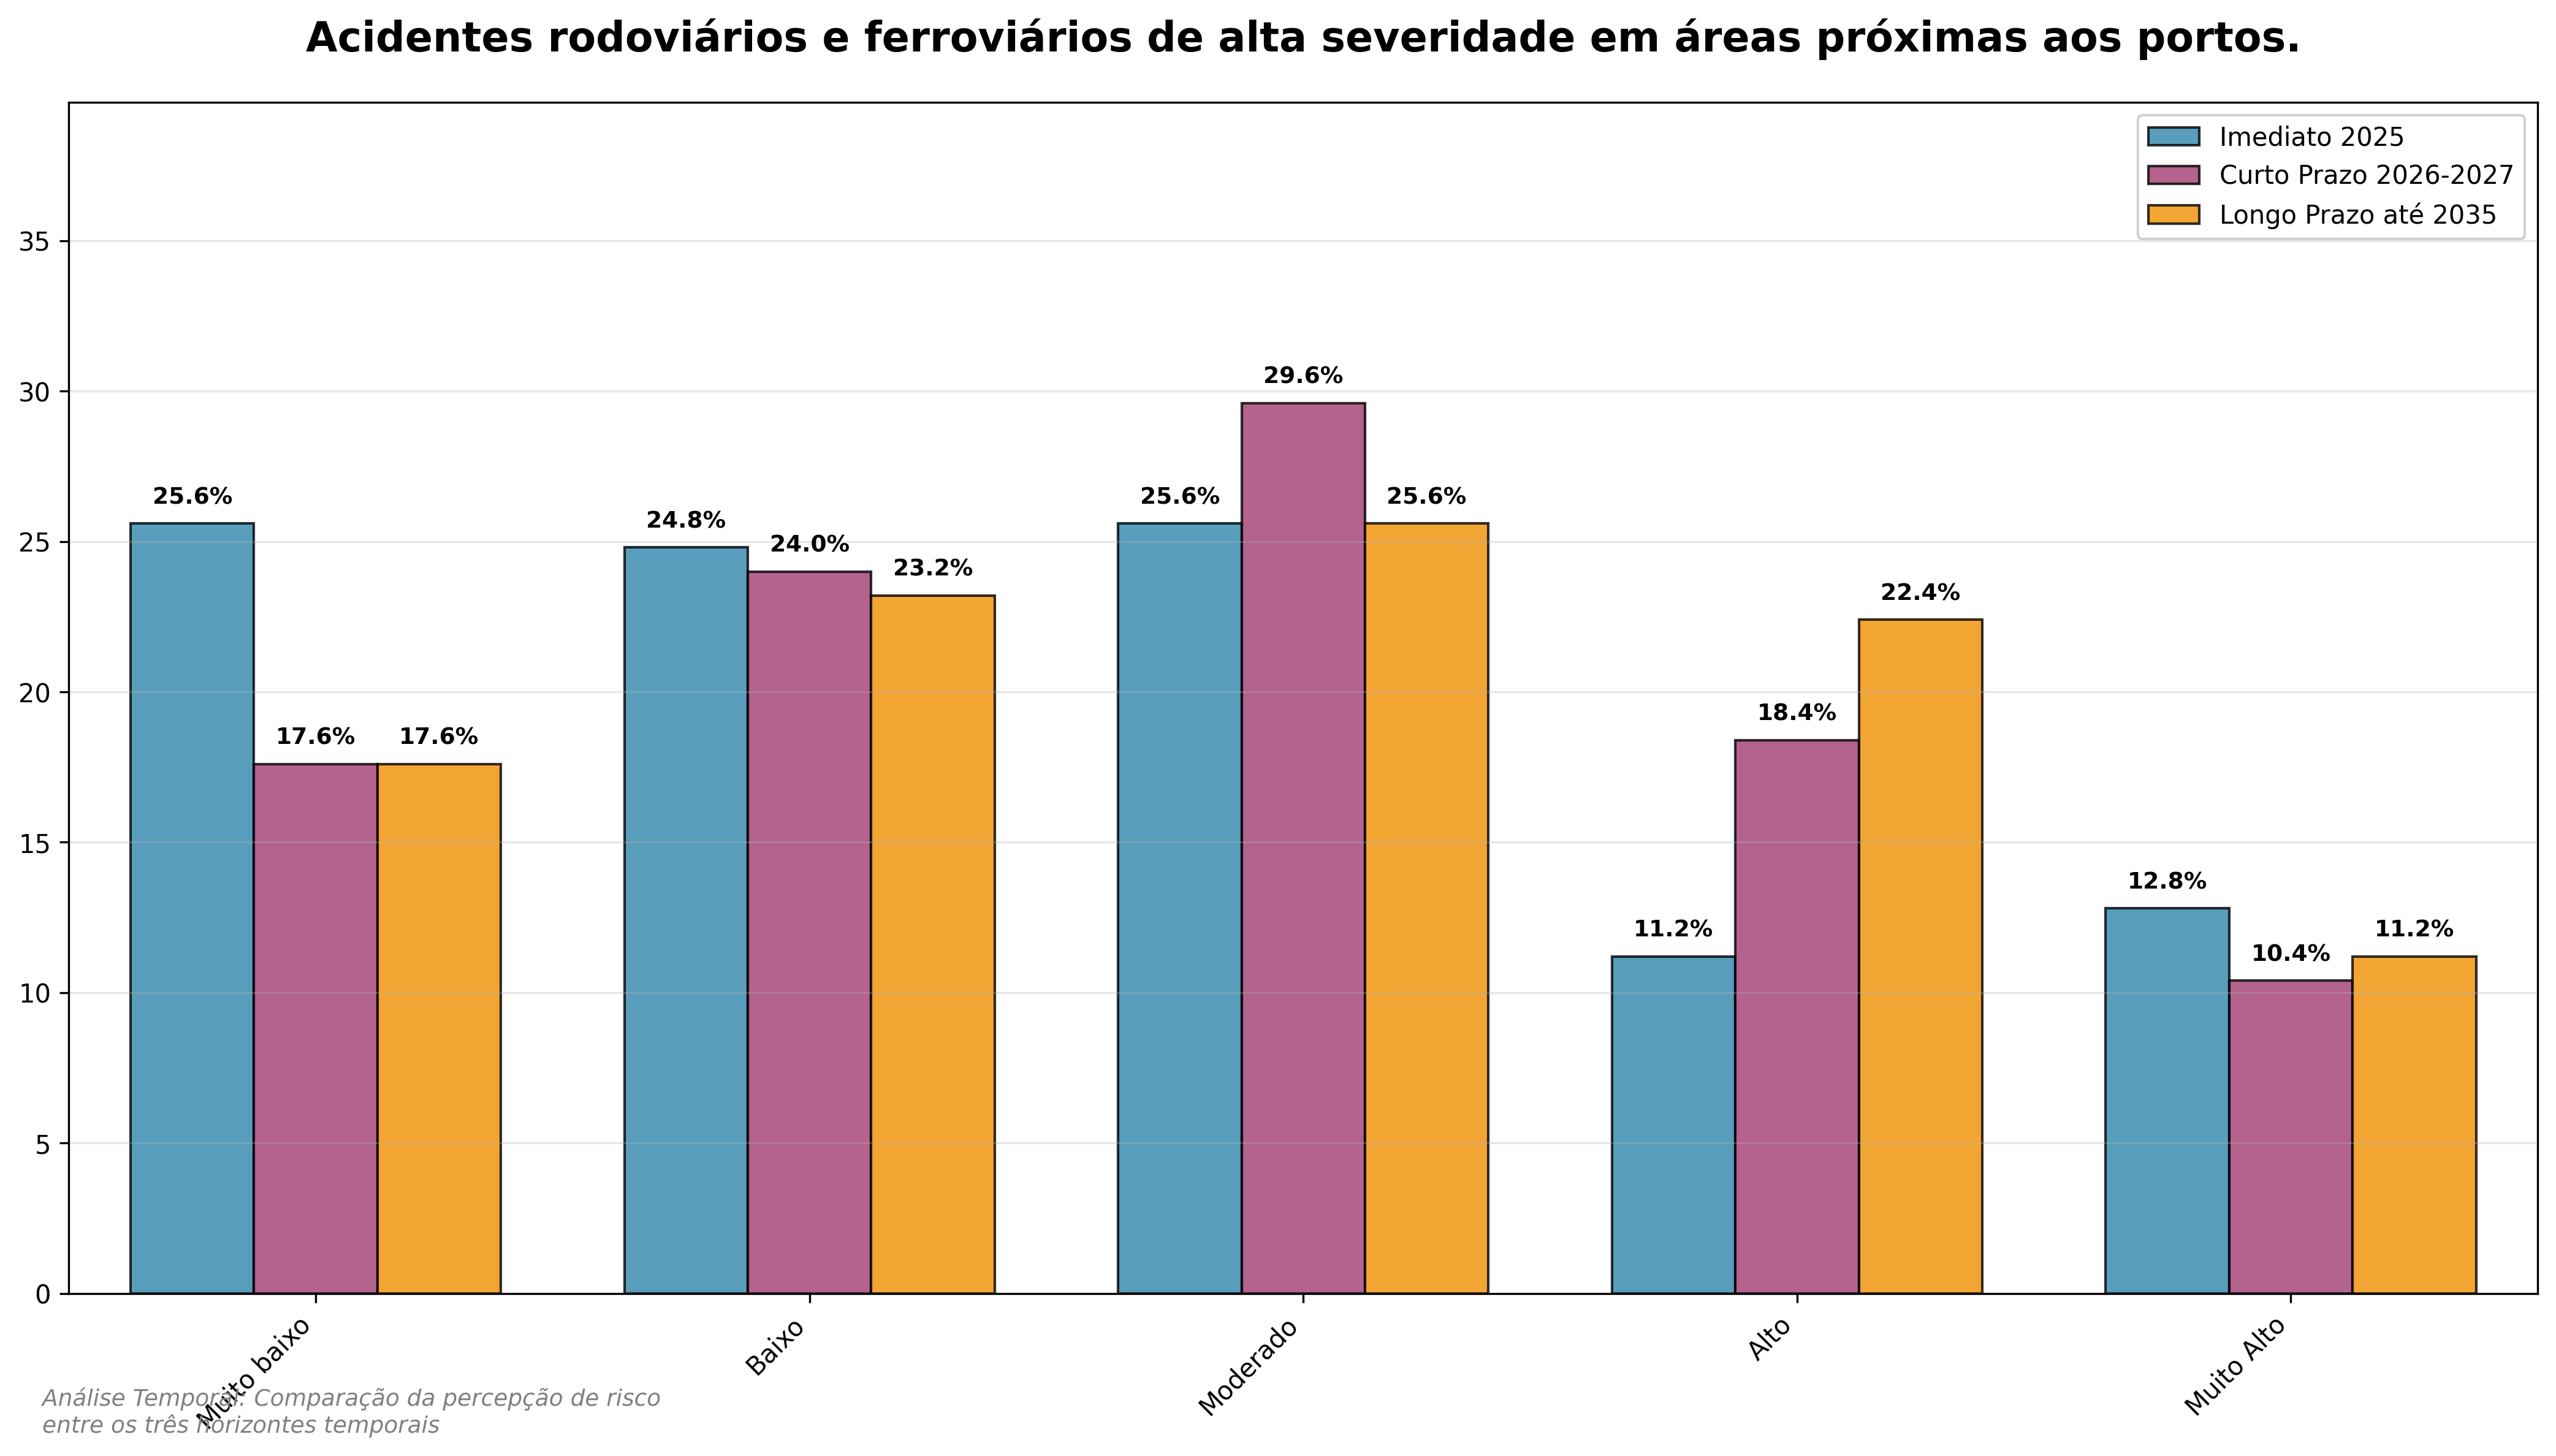
\includegraphics[keepaspectratio]{assets/social/grafico_agrupado_4_5_temporal.png}}

\begin{tcolorbox}[enhanced jigsaw, titlerule=0mm, colback=white, title=\textcolor{quarto-callout-note-color}{\faInfo}\hspace{0.5em}{Destaque}, opacityback=0, colbacktitle=quarto-callout-note-color!10!white, leftrule=.75mm, left=2mm, colframe=quarto-callout-note-color-frame, bottomrule=.15mm, bottomtitle=1mm, breakable, toprule=.15mm, toptitle=1mm, opacitybacktitle=0.6, arc=.35mm, coltitle=black, rightrule=.15mm]

\textbf{Evolução da Percepção de Risco:}

- \textbf{Tendência de crescimento moderado}: Aumento gradual da
preocupação

- \textbf{Mediana}: Evolui de 2.0 (2025) para 3.0 (2035)

- \textbf{Risco Alto (níveis 4-5)}: Cresce de 24\% (2025) para 34\%
(2035) - aumento de 40\%

- \textbf{Risco Baixo (níveis 1-2)}: Redução de 52\% (2025) para 37\%
(2035)

\textbf{Contexto Detalhado por Período:}

\textbf{Período Imediato 2025:} Devido aos acidentes rodoviários e
ferroviários de alta severidade próximos aos portos, poderá acontecer
bloqueios de acesso, danos a cargas perigosas e sinistros ambientais de
grande escala, o que poderá levar a rupturas na cadeia de suprimentos,
multas ambientais e perdas financeiras impactando a continuidade
logística e o cumprimento de SLAs estratégicos. No período imediato
2025, 24\% das respostas permanecem nos níveis 4-5 e a mediana em 2
indica um nível controlado sob vigilância.

\textbf{Período Curto Prazo 2026-2027:} A preocupação com acidentes
evolui para um nível moderado com tendência de crescimento, atingindo
29\% das respostas nos níveis 4-5 com mediana em 3, indicando transição
para risco elevado.

\textbf{Período Longo Prazo até 2035:} A situação se torna mais crítica,
com 34\% das respostas nos níveis 4-5 e mediana em 3, configurando um
nível elevado que demanda planos de ação priorizados.

\textbf{Implicações Estratégicas:} A crescente preocupação com acidentes
logísticos exige investimentos em segurança viária, sistemas de
monitoramento e planos de resposta emergenciais integrados. A evolução
de controlado para elevado indica necessidade de medidas preventivas
escalonadas ao longo do tempo.

\end{tcolorbox}

\subsection{Acidentes nas operações
portuárias}\label{acidentes-nas-operauxe7uxf5es-portuuxe1rias}

O gr?fico a seguir apresenta a evolu??o temporal do risco Acidentes nas
operações portuárias.
\pandocbounded{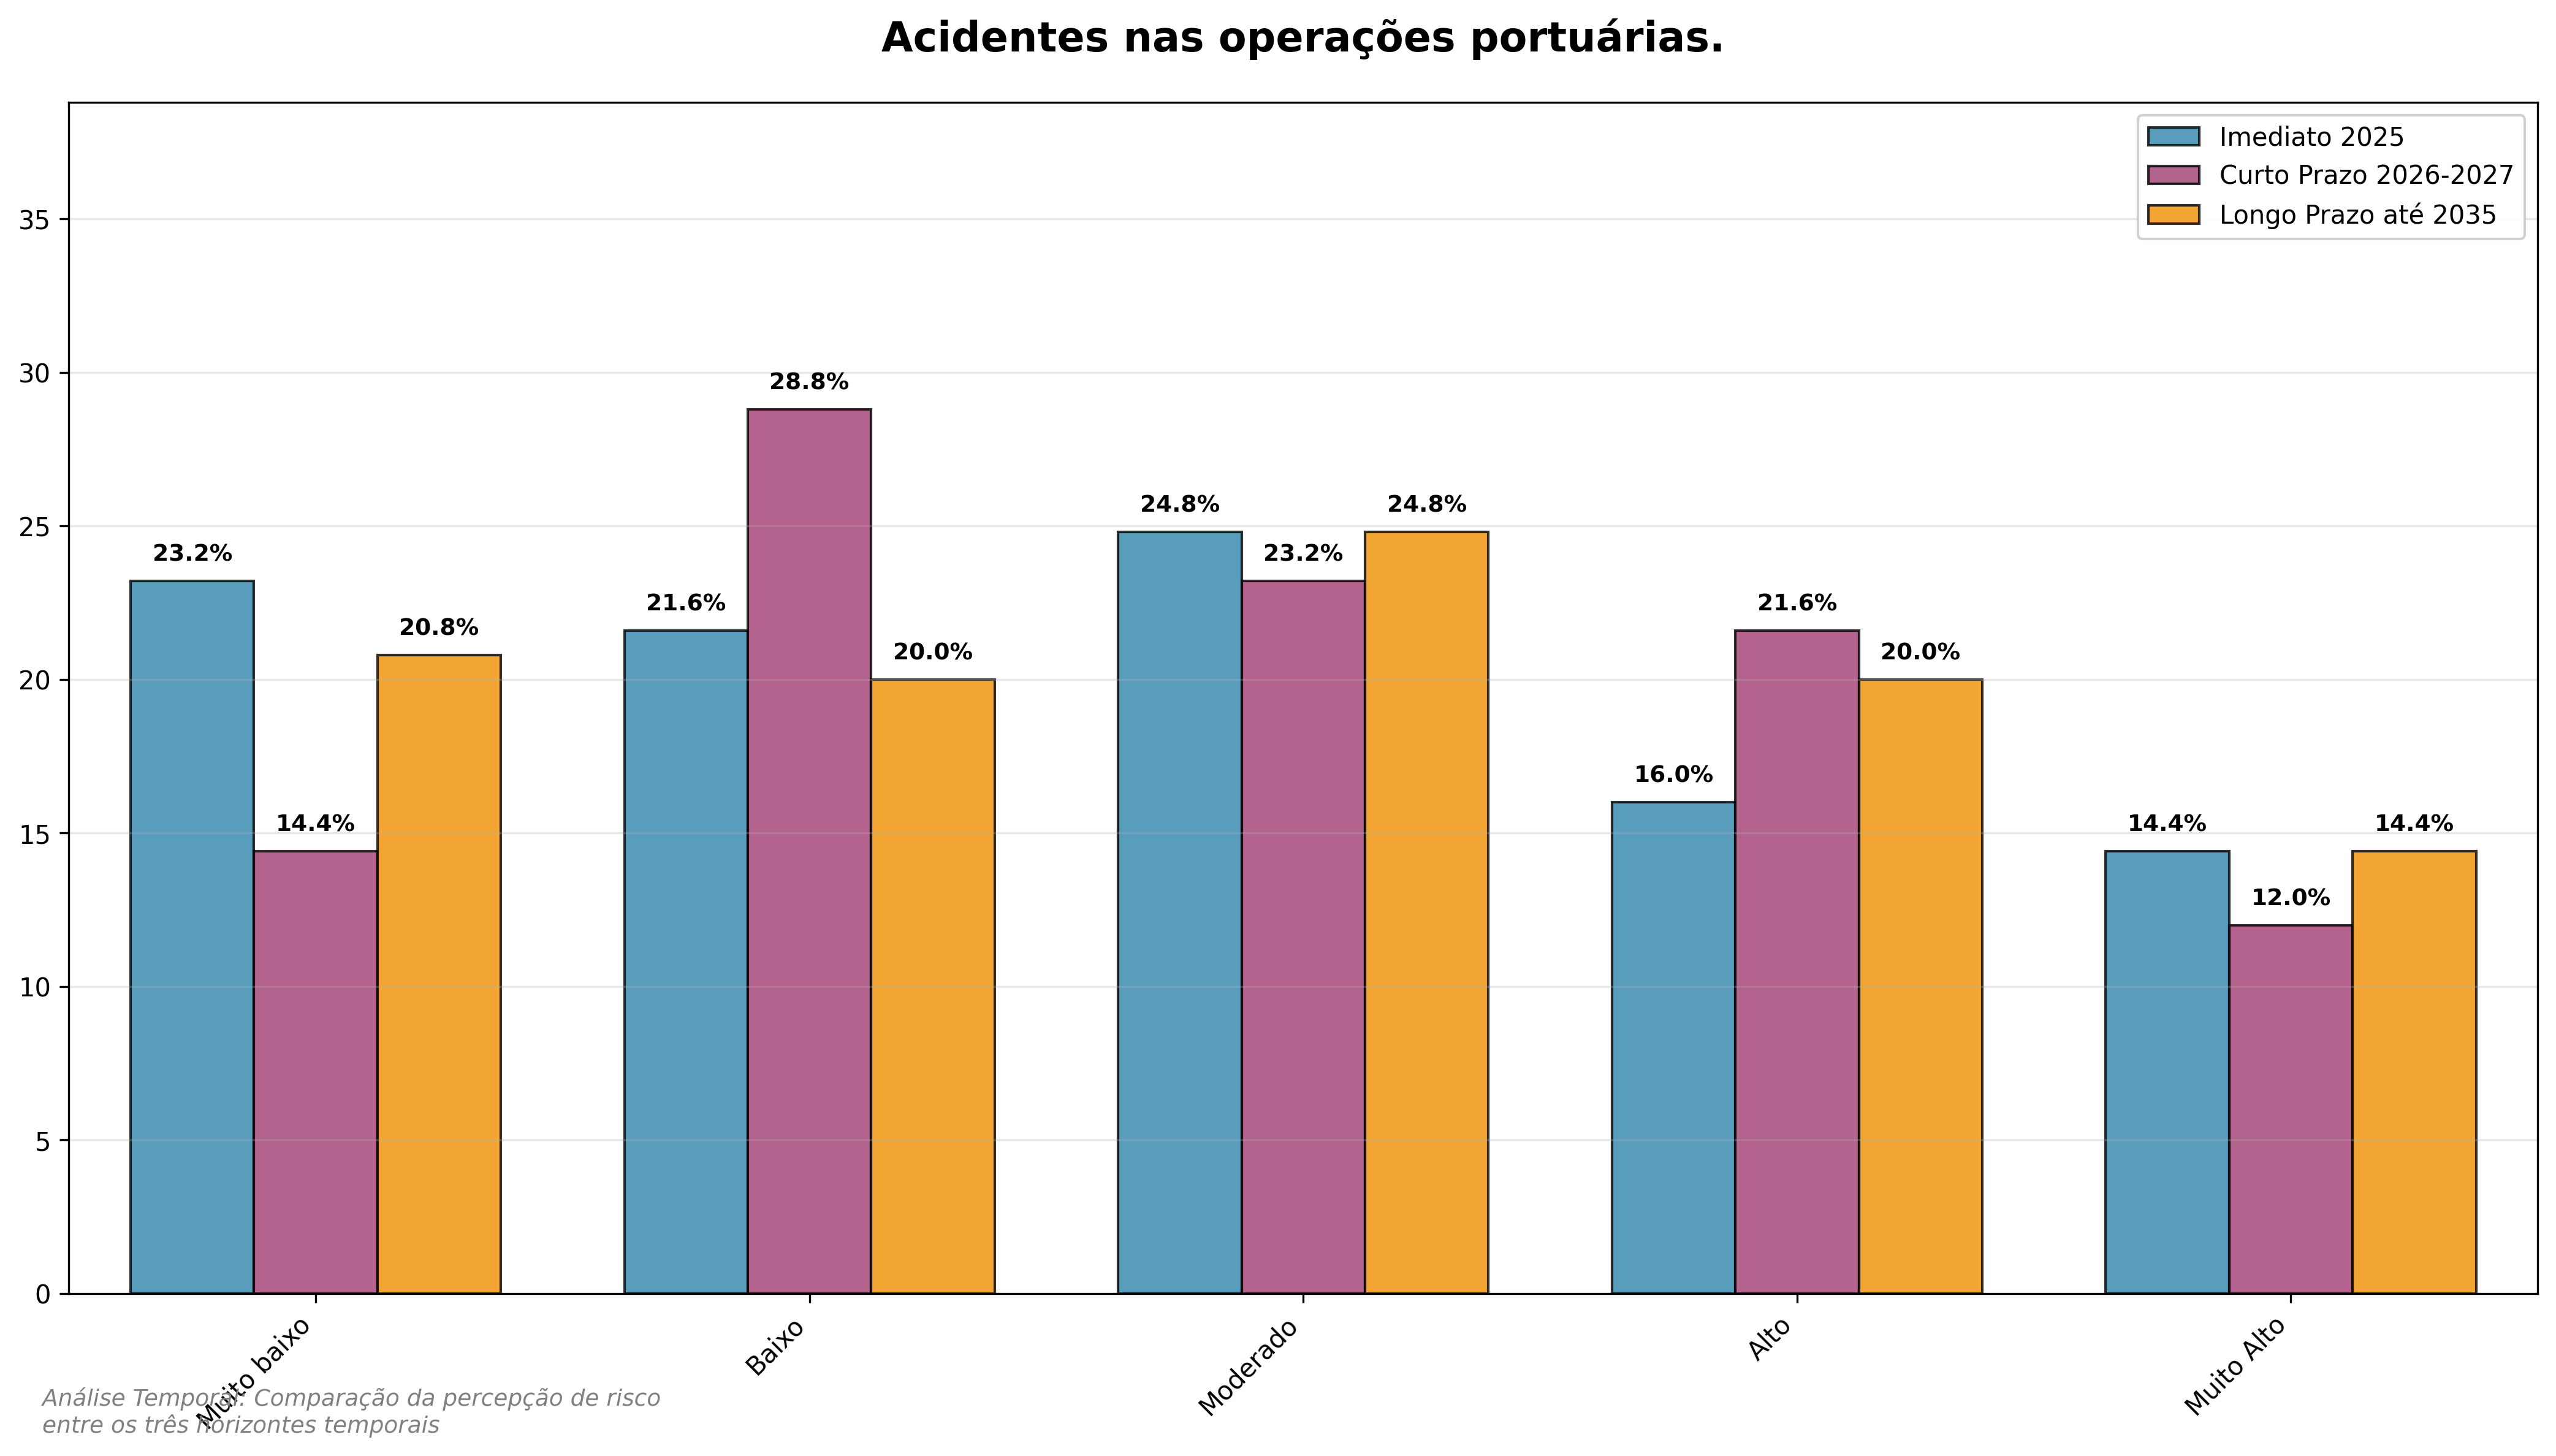
\includegraphics[keepaspectratio]{assets/social/grafico_agrupado_4_6_temporal.png}}

\begin{tcolorbox}[enhanced jigsaw, titlerule=0mm, colback=white, title=\textcolor{quarto-callout-note-color}{\faInfo}\hspace{0.5em}{Destaque}, opacityback=0, colbacktitle=quarto-callout-note-color!10!white, leftrule=.75mm, left=2mm, colframe=quarto-callout-note-color-frame, bottomrule=.15mm, bottomtitle=1mm, breakable, toprule=.15mm, toptitle=1mm, opacitybacktitle=0.6, arc=.35mm, coltitle=black, rightrule=.15mm]

\textbf{Evolução da Percepção de Risco:}

- \textbf{Tendência de elevação consistente}: Preocupação crescente com
segurança operacional

- \textbf{Mediana}: Mantém-se em 3.0 em todos os períodos, indicando
risco persistente

- \textbf{Risco Alto (níveis 4-5)}: Cresce de 30\% (2025) para 34\%
(2035) - aumento de 13\%

- \textbf{Risco Baixo (níveis 1-2)}: Redução de 37\% (2025) para 32\%
(2035)

\textbf{Contexto Detalhado por Período:}

\textbf{Período Imediato 2025:} Devido aos acidentes nas operações
portuárias, poderá acontecer falhas em equipamentos, incidentes com
trabalhadores e paradas de berço, o que poderá levar a interrupção das
operações, indenizações e investigações regulatórias impactando a
produtividade operacional e a segurança do trabalho. No período imediato
2025, 30\% das respostas permanecem nos níveis 4-5 e a mediana em 3
indica um nível elevado que demanda planos de ação priorizados.

\textbf{Período Curto Prazo 2026-2027:} A preocupação com acidentes
operacionais se mantém elevada, atingindo 34\% das respostas nos níveis
4-5 com mediana em 3, configurando um patamar crítico que exige atenção
contínua.

\textbf{Período Longo Prazo até 2035:} A situação persiste como crítica,
com 34\% das respostas nos níveis 4-5 e mediana em 3, indicando um risco
elevado e persistente que requer investimentos contínuos.

\textbf{Implicações Estratégicas:} Acidentes operacionais representam um
risco crítico e persistente que exige investimentos contínuos em
treinamento, equipamentos e cultura de segurança. A persistência do
risco em todos os períodos indica necessidade de melhorias sistêmicas e
culturais na segurança operacional.

\end{tcolorbox}

\subsection{Falhas na gestão de crises e na resposta a
emergências}\label{falhas-na-gestuxe3o-de-crises-e-na-resposta-a-emerguxeancias}

O gr?fico a seguir apresenta a evolu??o temporal do risco Falhas na
gestão de crises e na resposta a emergências.
\pandocbounded{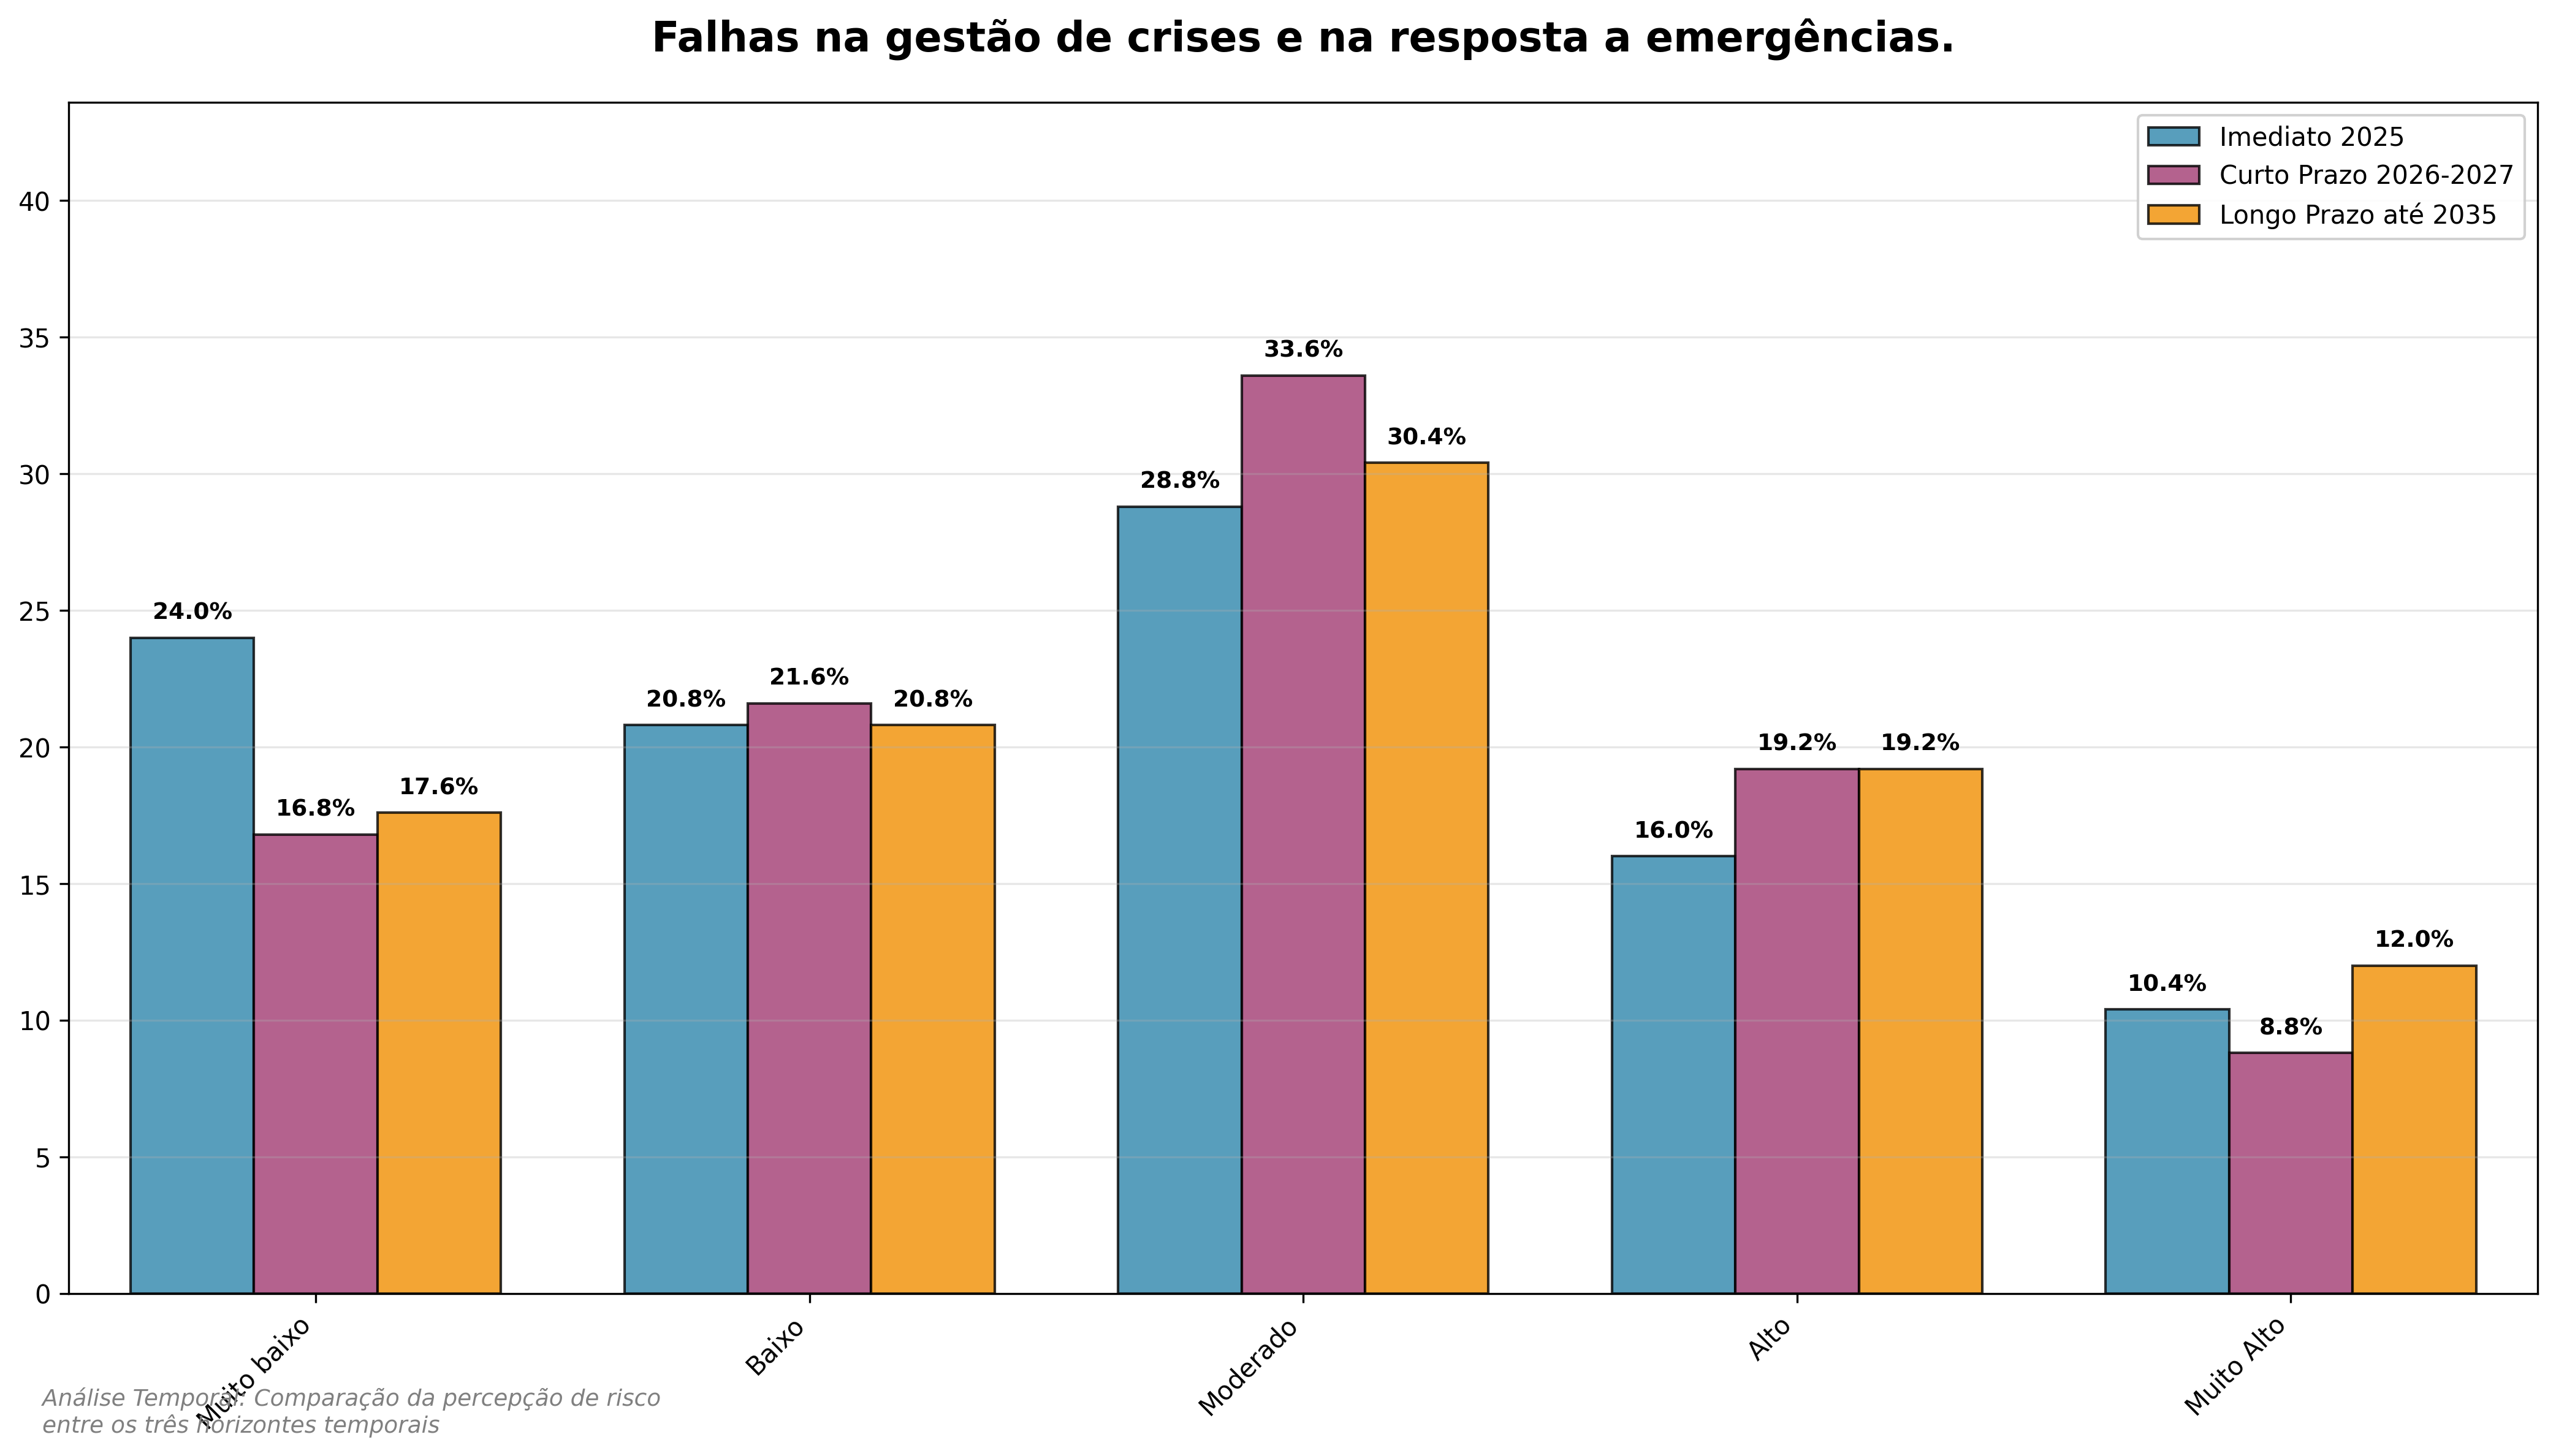
\includegraphics[keepaspectratio]{assets/social/grafico_agrupado_4_7_temporal.png}}

\begin{tcolorbox}[enhanced jigsaw, titlerule=0mm, colback=white, title=\textcolor{quarto-callout-note-color}{\faInfo}\hspace{0.5em}{Destaque}, opacityback=0, colbacktitle=quarto-callout-note-color!10!white, leftrule=.75mm, left=2mm, colframe=quarto-callout-note-color-frame, bottomrule=.15mm, bottomtitle=1mm, breakable, toprule=.15mm, toptitle=1mm, opacitybacktitle=0.6, arc=.35mm, coltitle=black, rightrule=.15mm]

\textbf{Evolução da Percepção de Risco:}

- \textbf{Tendência de crescimento moderado}: Aumento da preocupação com
capacidade de resposta

- \textbf{Mediana}: Mantém-se em 3.0 em todos os períodos

- \textbf{Risco Alto (níveis 4-5)}: Cresce de 26\% (2025) para 31\%
(2035) - aumento de 18\%

- \textbf{Risco Baixo (níveis 1-2)}: Redução de 41\% (2025) para 33\%
(2035)

\textbf{Contexto Detalhado por Período:}

\textbf{Período Imediato 2025:} Devido às falhas na gestão de crises e
na resposta a emergências, poderá acontecer atrasos em planos de
contingência e comunicações desencontradas durante incidentes, o que
poderá levar a perda de tempo de resposta, ampliação de danos e
responsabilizações legais impactando a resiliência institucional e a
proteção de vidas e ativos. No período imediato 2025, 26\% das respostas
permanecem nos níveis 4-5 e a mediana em 3 indica um nível moderado com
tendência de crescimento.

\textbf{Período Curto Prazo 2026-2027:} A preocupação com gestão de
crises se mantém elevada, atingindo 28\% das respostas nos níveis 4-5
com mediana em 3, configurando um patamar crítico que exige atenção
contínua.

\textbf{Período Longo Prazo até 2035:} A situação se torna mais crítica,
com 31\% das respostas nos níveis 4-5 e mediana em 3, indicando um risco
elevado e persistente que requer investimentos contínuos.

\textbf{Implicações Estratégicas:} A gestão de crises requer
investimentos em planos de contingência, treinamento regular e sistemas
de comunicação robustos para garantir resposta efetiva. A persistência
do risco em todos os períodos indica necessidade de melhorias sistêmicas
na capacidade de resposta emergencial.

\end{tcolorbox}

\subsection{Falhas no controle interno: fraudes ou
corrupção}\label{falhas-no-controle-interno-fraudes-ou-corrupuxe7uxe3o}

O gr?fico a seguir apresenta a evolu??o temporal do risco Falhas no
controle interno: fraudes ou corrupção.
\pandocbounded{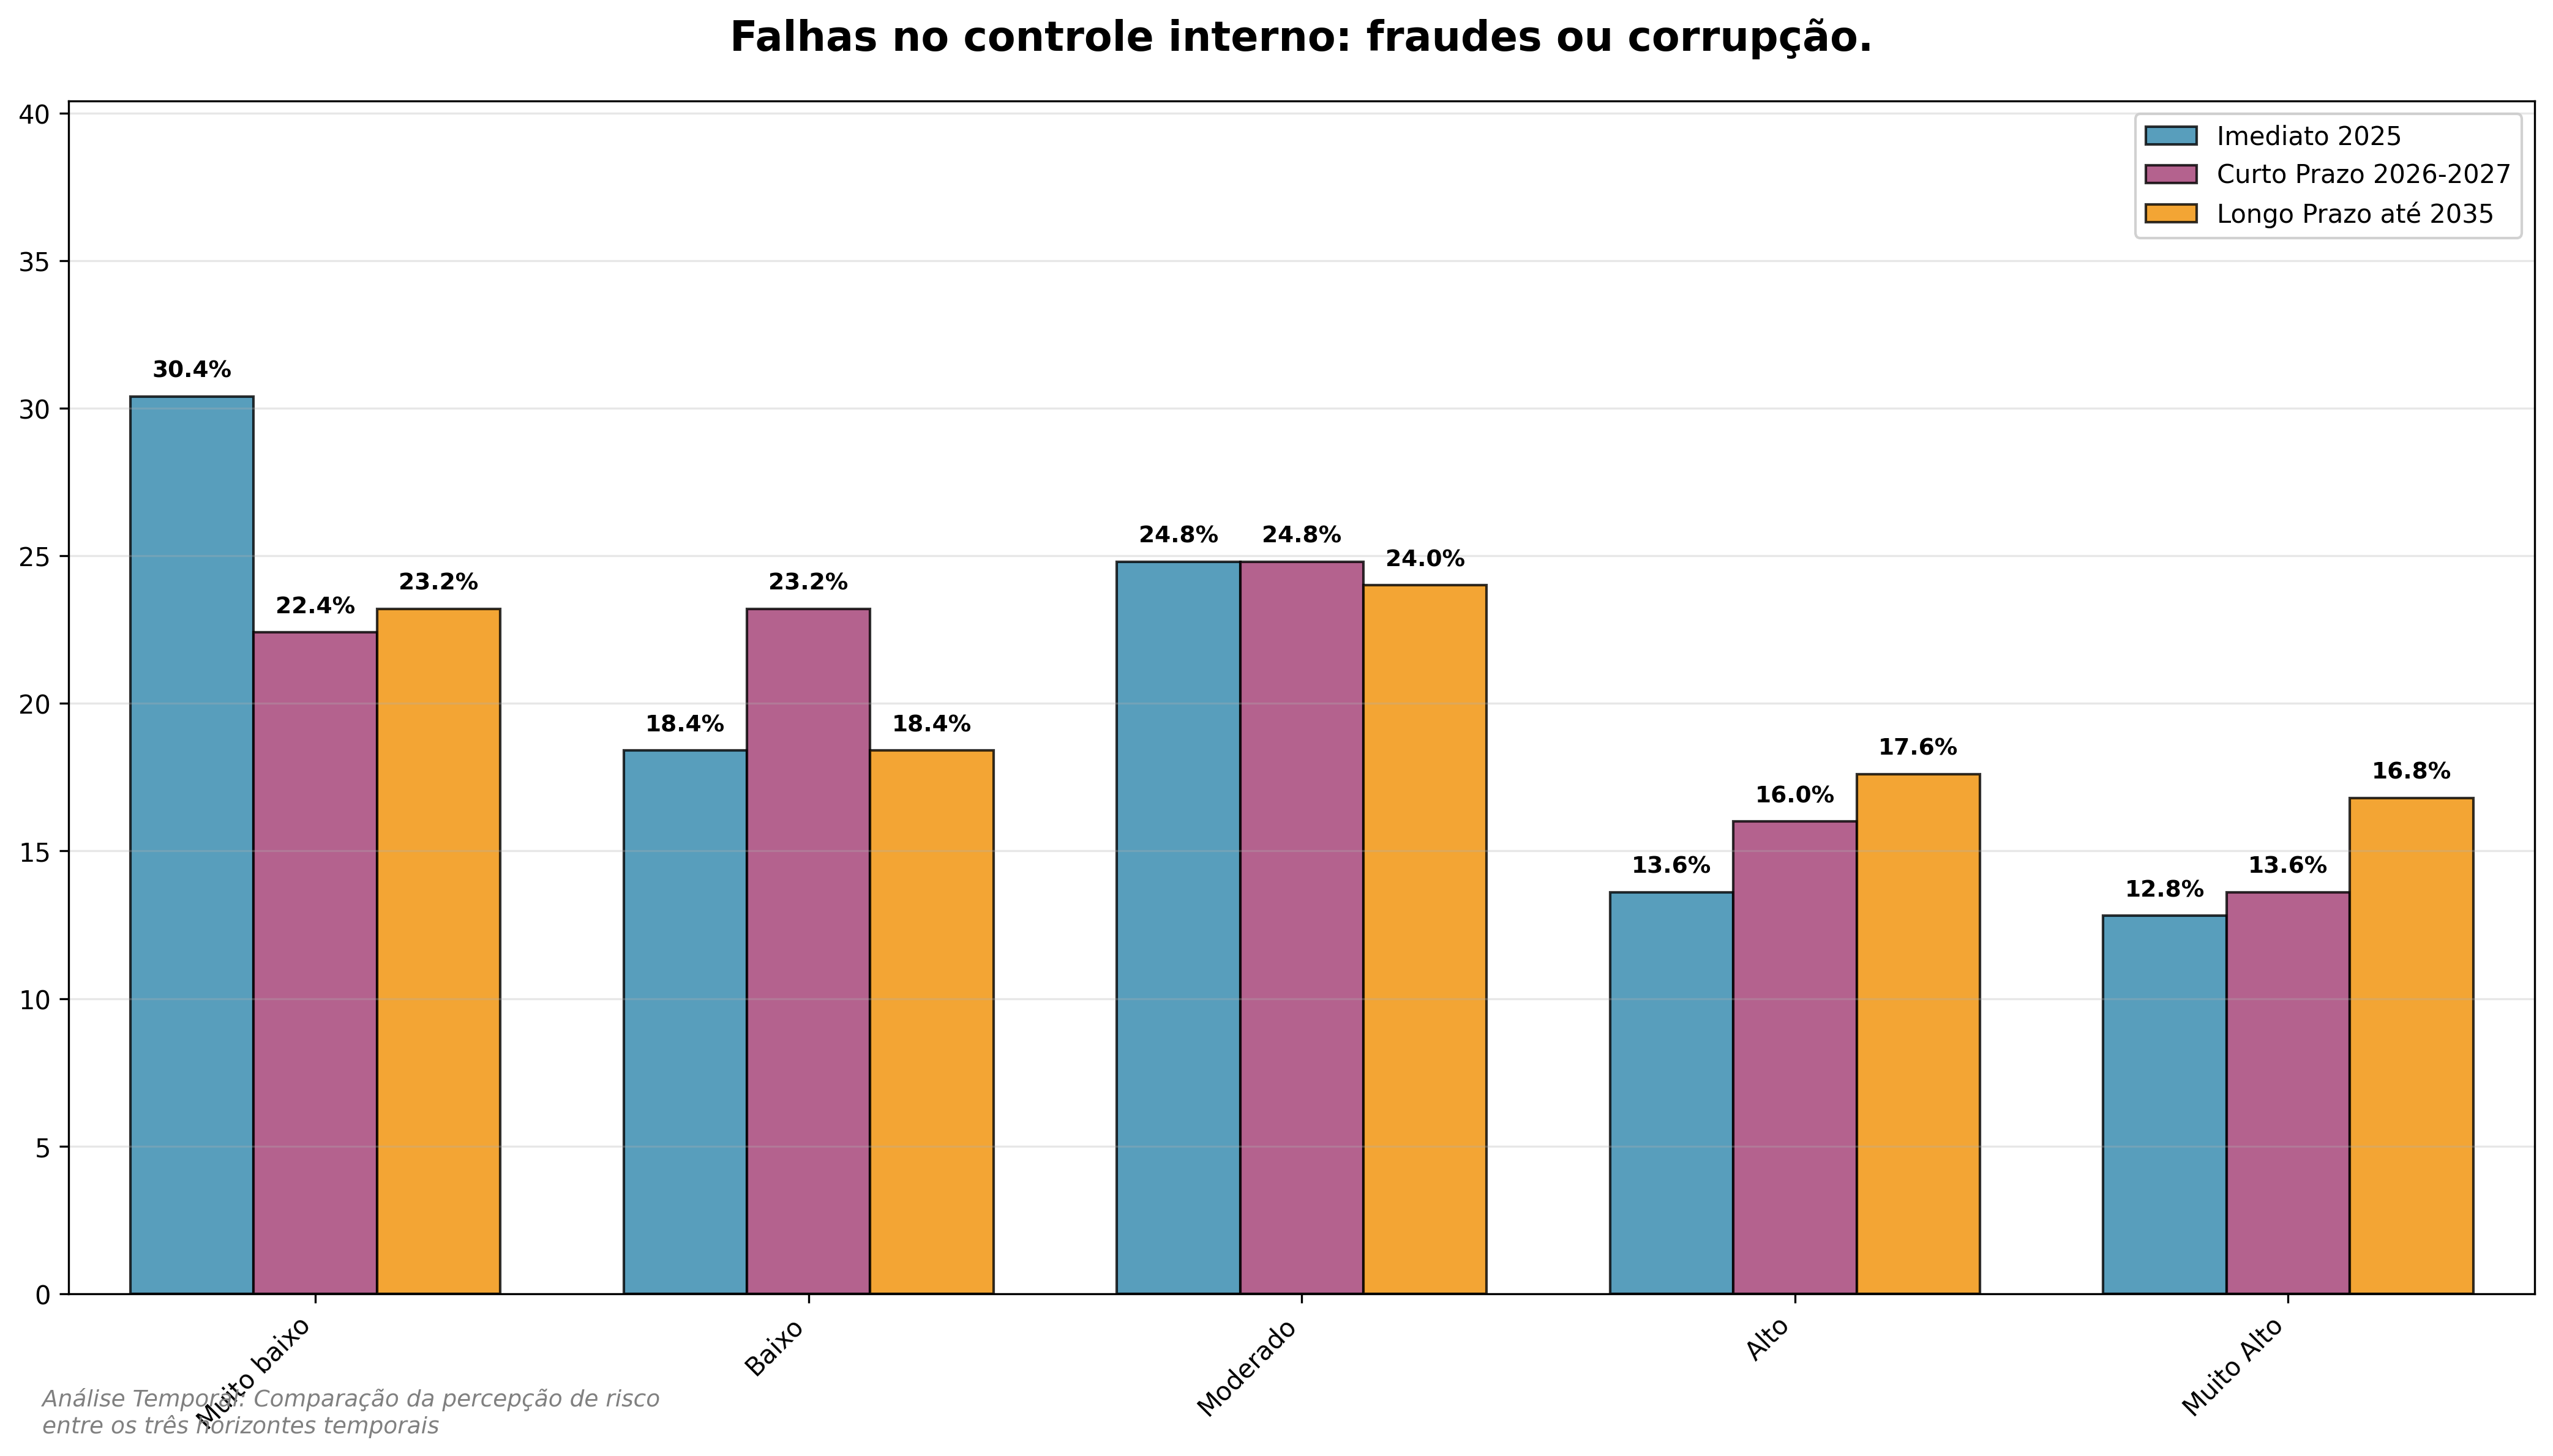
\includegraphics[keepaspectratio]{assets/social/grafico_agrupado_4_8_temporal.png}}

\begin{tcolorbox}[enhanced jigsaw, titlerule=0mm, colback=white, title=\textcolor{quarto-callout-note-color}{\faInfo}\hspace{0.5em}{Destaque}, opacityback=0, colbacktitle=quarto-callout-note-color!10!white, leftrule=.75mm, left=2mm, colframe=quarto-callout-note-color-frame, bottomrule=.15mm, bottomtitle=1mm, breakable, toprule=.15mm, toptitle=1mm, opacitybacktitle=0.6, arc=.35mm, coltitle=black, rightrule=.15mm]

\textbf{Evolução da Percepção de Risco:}

- \textbf{Tendência de crescimento significativo}: Preocupação crescente
com governança

- \textbf{Mediana}: Mantém-se em 3.0 em todos os períodos

- \textbf{Risco Alto (níveis 4-5)}: Cresce de 26\% (2025) para 34\%
(2035) - aumento de 30\%

- \textbf{Risco Baixo (níveis 1-2)}: Redução de 41\% (2025) para 32\%
(2035)

\textbf{Contexto Detalhado por Período:}

\textbf{Período Imediato 2025:} Devido às falhas no controle interno,
fraudes ou corrupção, poderá acontecer desvios de recursos, contratos
irregulares e sanções dos órgãos de controle, o que poderá levar a
multas, perda de confiança e restrições ao acesso a financiamentos
impactando a governança corporativa e a sustentabilidade financeira. No
período imediato 2025, 26\% das respostas permanecem nos níveis 4-5 e a
mediana em 3 indica um nível moderado com tendência de crescimento.

\textbf{Período Curto Prazo 2026-2027:} A preocupação com falhas no
controle interno se mantém elevada, atingindo 30\% das respostas nos
níveis 4-5 com mediana em 3, configurando um patamar crítico que exige
atenção contínua.

\textbf{Período Longo Prazo até 2035:} A situação se torna mais crítica,
com 34\% das respostas nos níveis 4-5 e mediana em 3, indicando um risco
elevado e persistente que requer investimentos contínuos.

\textbf{Implicações Estratégicas:} Riscos de governança exigem
fortalecimento de controles internos, auditorias regulares e cultura
organizacional ética para mitigar fraudes e corrupção. A evolução de
moderado para elevado indica necessidade de melhorias sistêmicas na
transparência e compliance.

\end{tcolorbox}

\subsection{Instabilidade gerada por alterações no marco regulatório e
excesso de
judicialização}\label{instabilidade-gerada-por-alterauxe7uxf5es-no-marco-regulatuxf3rio-e-excesso-de-judicializauxe7uxe3o}

O gr?fico a seguir apresenta a evolu??o temporal do risco Instabilidade
gerada por alterações no marco regulatório e excesso de judicialização.
\pandocbounded{
\includegraphics[keepaspectratio]{assets/social/grafico_agrupado_4_9_temporal.png}}

\begin{tcolorbox}[enhanced jigsaw, titlerule=0mm, colback=white, title=\textcolor{quarto-callout-note-color}{\faInfo}\hspace{0.5em}{Destaque}, opacityback=0, colbacktitle=quarto-callout-note-color!10!white, leftrule=.75mm, left=2mm, colframe=quarto-callout-note-color-frame, bottomrule=.15mm, bottomtitle=1mm, breakable, toprule=.15mm, toptitle=1mm, opacitybacktitle=0.6, arc=.35mm, coltitle=black, rightrule=.15mm]

\textbf{Evolução da Percepção de Risco:}

\begin{itemize}
\tightlist
\item
  \textbf{Risco estrutural}: percentuais em níveis 4-5 ficam acima de
  34\% em todos os horizontes e alcançam 40\% em 2035;-
  \textbf{Mediana}: permanece em 3,0, reforçando que o risco já é
  tratado como elevado hoje;- \textbf{Risco baixo (níveis 1-2)}: cai de
  37\% para 34\%, sinalizando perda gradual de confiança regulatória.
  \textbf{Contexto Detalhado por Período:}
\end{itemize}

\textbf{Período Imediato 2025:} Mediana 3, risco alto em 34\% e baixo em
37\% mostram ambiente ainda dividido, mas já pressionado por mudanças
legislativas e disputas judiciais que afetam concessões, licenças e
contratos.

\textbf{Período Curto Prazo 2026-2027:} O percentual em níveis 4-5
avança para 38\% com redução do grupo de baixo risco para 36\%,
refletindo expectativas de revisões normativas frequentes e maior
litigiosidade envolvendo operações portuárias.

\textbf{Período Longo Prazo até 2035:} A instabilidade torna-se crônica:
40\% das respostas em risco alto e apenas 34\% em risco baixo apontam
para um ciclo prolongado de disputas regulatórias e judicialização de
investimentos.

\textbf{Implicações Estratégicas:} Portos e terminais precisam reforçar
governança regulatória, monitoramento legislativo e estratégias de
advocacy, além de estruturar equipes jurídicas e de compliance capazes
de antecipar mudanças. Contratos mais resilientes, matrizes de riscos
regulatórios e engajamento contínuo com entes públicos reduzem a
probabilidade de paralisações e multas.

\end{tcolorbox}

\subsection{Falta de recursos humanos capacitados e especializados no
setor
portuário}\label{falta-de-recursos-humanos-capacitados-e-especializados-no-setor-portuuxe1rio}

O gr?fico a seguir apresenta a evolu??o temporal do risco Falta de
recursos humanos capacitados e especializados no setor portuário.
\pandocbounded{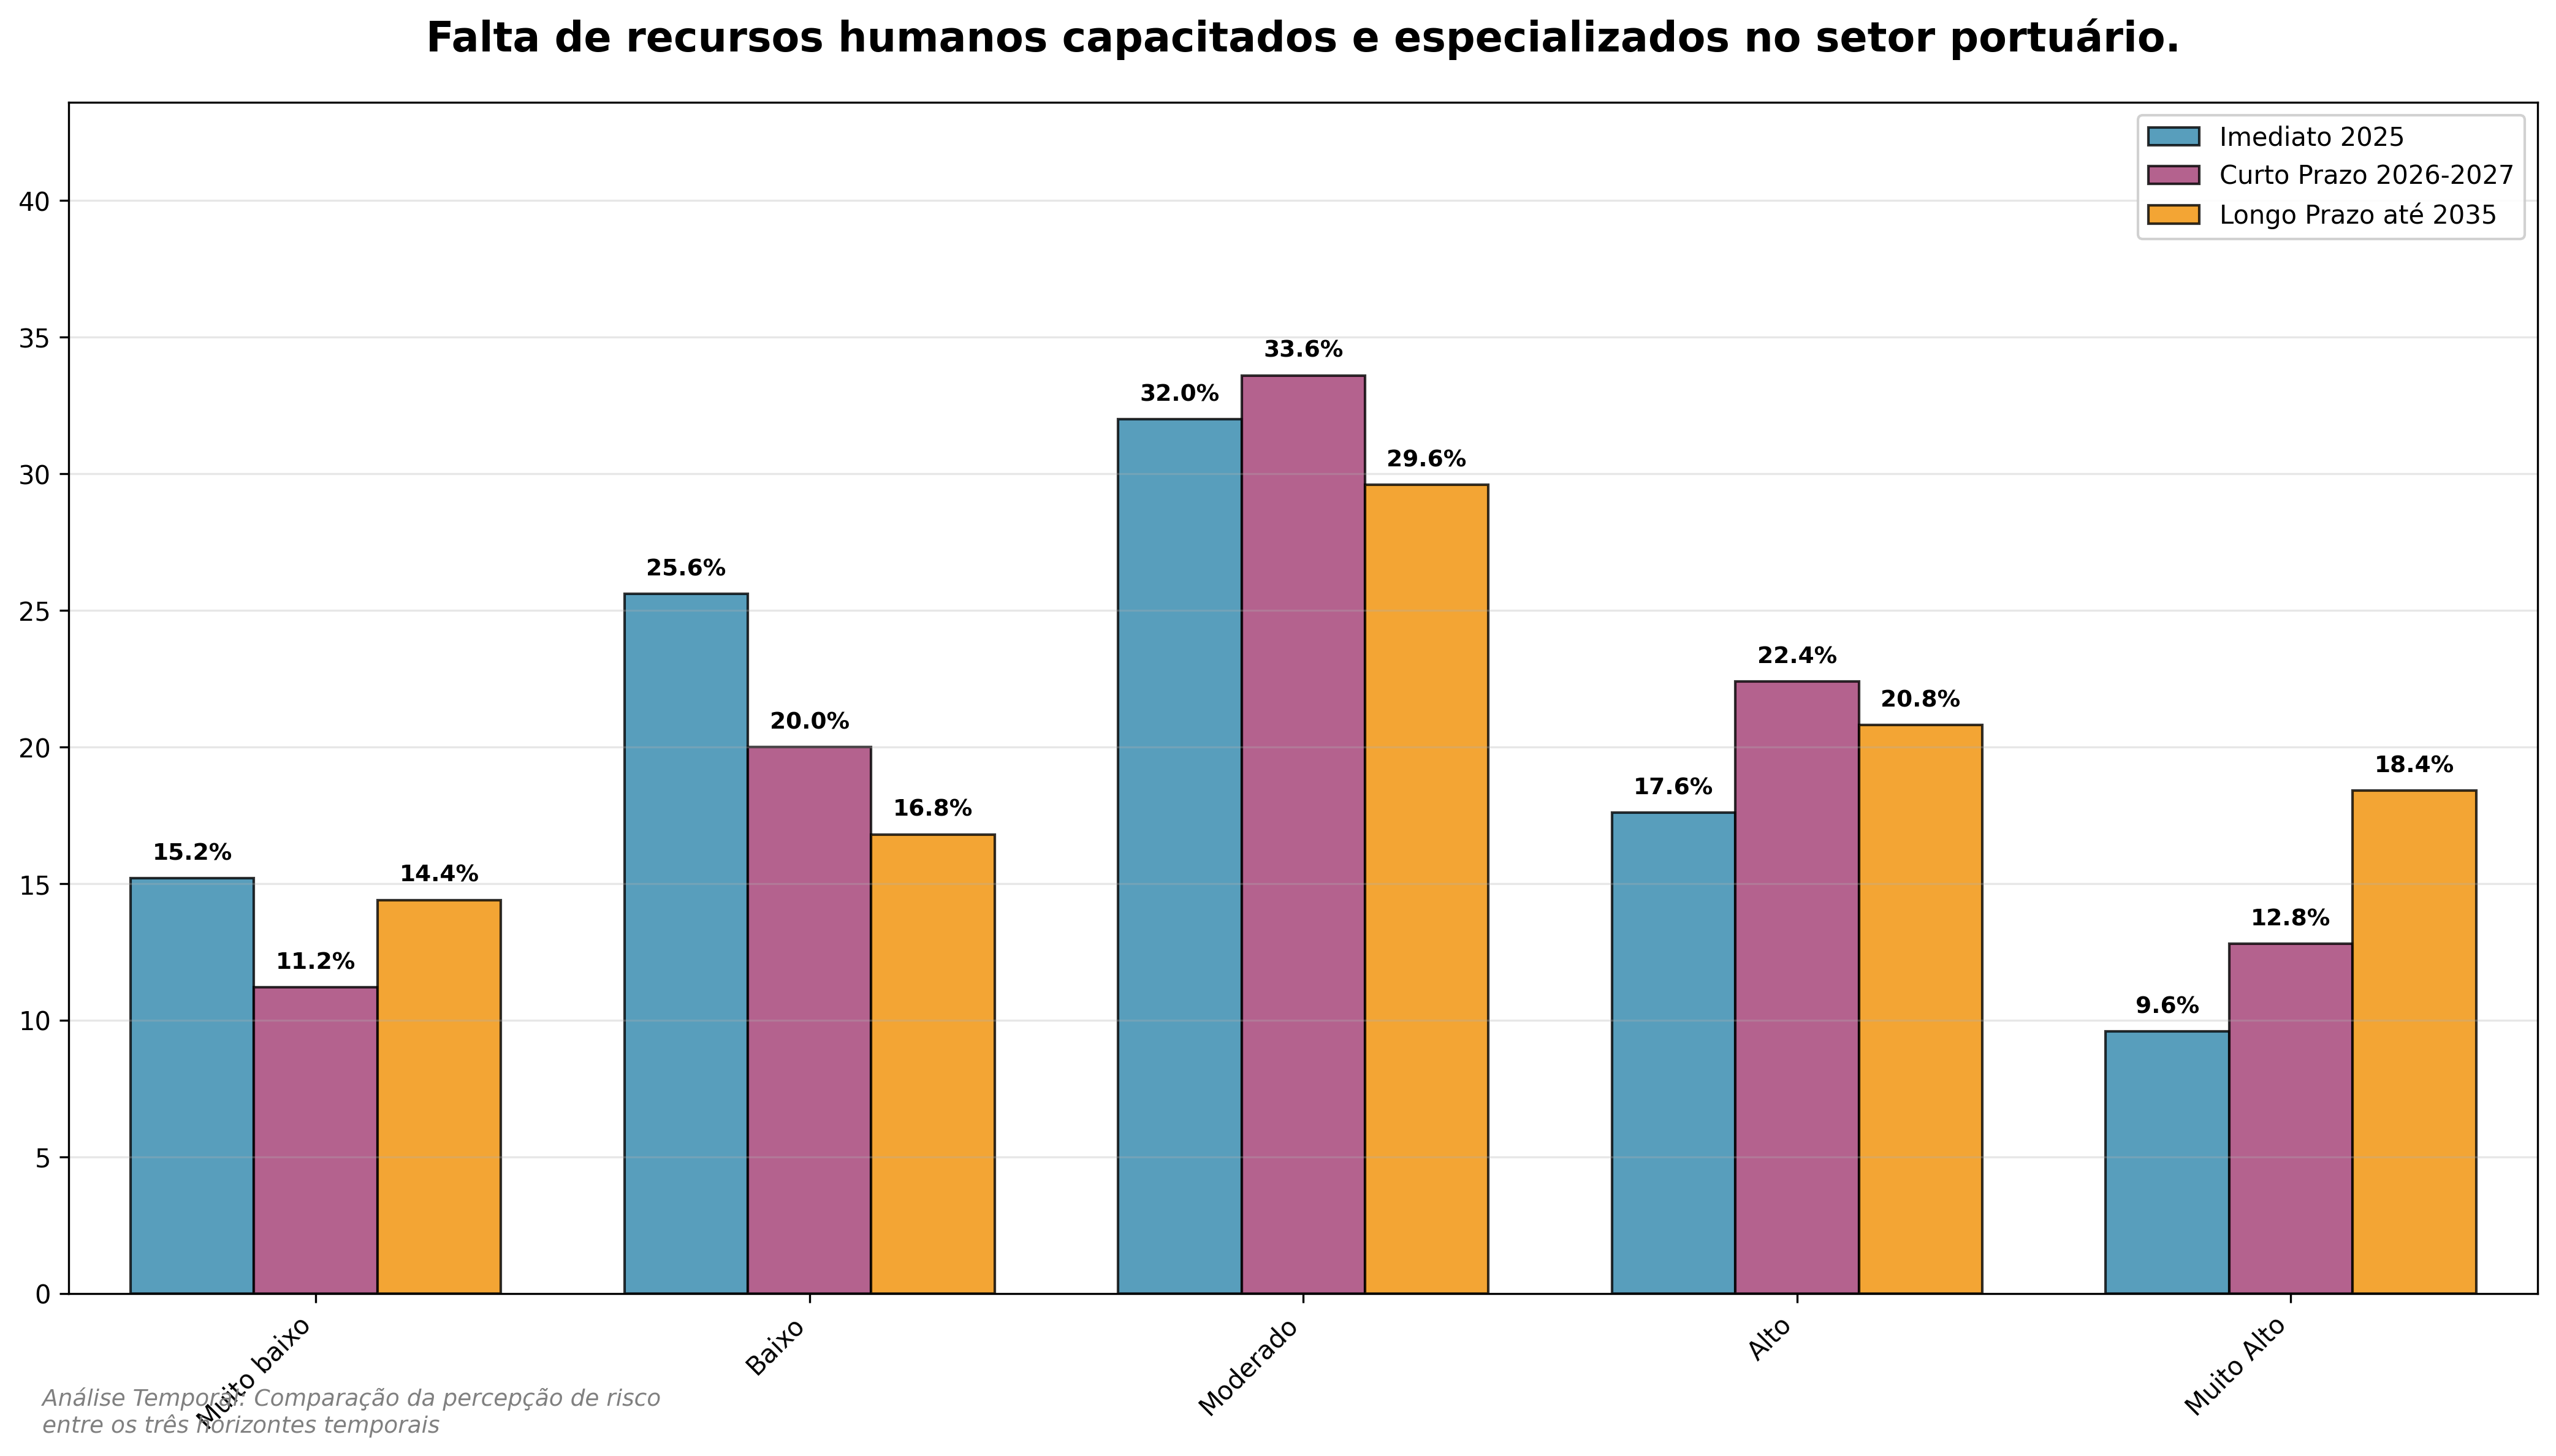
\includegraphics[keepaspectratio]{assets/social/grafico_agrupado_4_10_temporal.png}}

\begin{tcolorbox}[enhanced jigsaw, titlerule=0mm, colback=white, title=\textcolor{quarto-callout-note-color}{\faInfo}\hspace{0.5em}{Destaque}, opacityback=0, colbacktitle=quarto-callout-note-color!10!white, leftrule=.75mm, left=2mm, colframe=quarto-callout-note-color-frame, bottomrule=.15mm, bottomtitle=1mm, breakable, toprule=.15mm, toptitle=1mm, opacitybacktitle=0.6, arc=.35mm, coltitle=black, rightrule=.15mm]

\textbf{Evolução da Percepção de Risco:}

- \textbf{Tendência de crescimento acentuado}: Preocupação crescente com
gap de competências

- \textbf{Mediana}: Mantém-se em 3.0 em todos os períodos

- \textbf{Risco Alto (níveis 4-5)}: Cresce de 27\% (2025) para 39\%
(2035) - aumento de 44\%

- \textbf{Risco Baixo (níveis 1-2)}: Redução de 37\% (2025) para 28\%
(2035)

\textbf{Contexto Detalhado por Período:}

\textbf{Período Imediato 2025:} Devido à falta de recursos humanos
capacitados e especializados no setor portuário, poderá acontecer
lacunas de competências técnicas e dificuldades de preencher turnos
estratégicos, o que poderá levar a queda de produtividade, atrasos
operacionais e dependência de terceiros impactando a eficiência
operacional e a preservação do conhecimento crítico. No período imediato
2025, 27\% das respostas permanecem nos níveis 4-5 e a mediana em 3
indica um nível moderado com tendência de crescimento.

\textbf{Período Curto Prazo 2026-2027:} A preocupação com recursos
humanos se intensifica, atingindo 35\% das respostas nos níveis 4-5 com
mediana em 3, configurando um nível elevado que demanda planos de ação
priorizados.

\textbf{Período Longo Prazo até 2035:} A situação se torna crítica, com
39\% das respostas nos níveis 4-5 e mediana em 3, indicando um risco
elevado e persistente que requer investimentos contínuos.

\textbf{Implicações Estratégicas:} A escassez de talentos exige
investimentos em programas de formação, parcerias educacionais e
estratégias de retenção para garantir sustentabilidade operacional. A
evolução de moderado para elevado indica necessidade de planejamento
estratégico de longo prazo para desenvolvimento de competências.

\end{tcolorbox}

\subsection{Assédio (moral e sexual) no ambiente de
trabalho}\label{assuxe9dio-moral-e-sexual-no-ambiente-de-trabalho}

O gr?fico a seguir apresenta a evolu??o temporal do risco Assédio (moral
e sexual) no ambiente de trabalho.
\pandocbounded{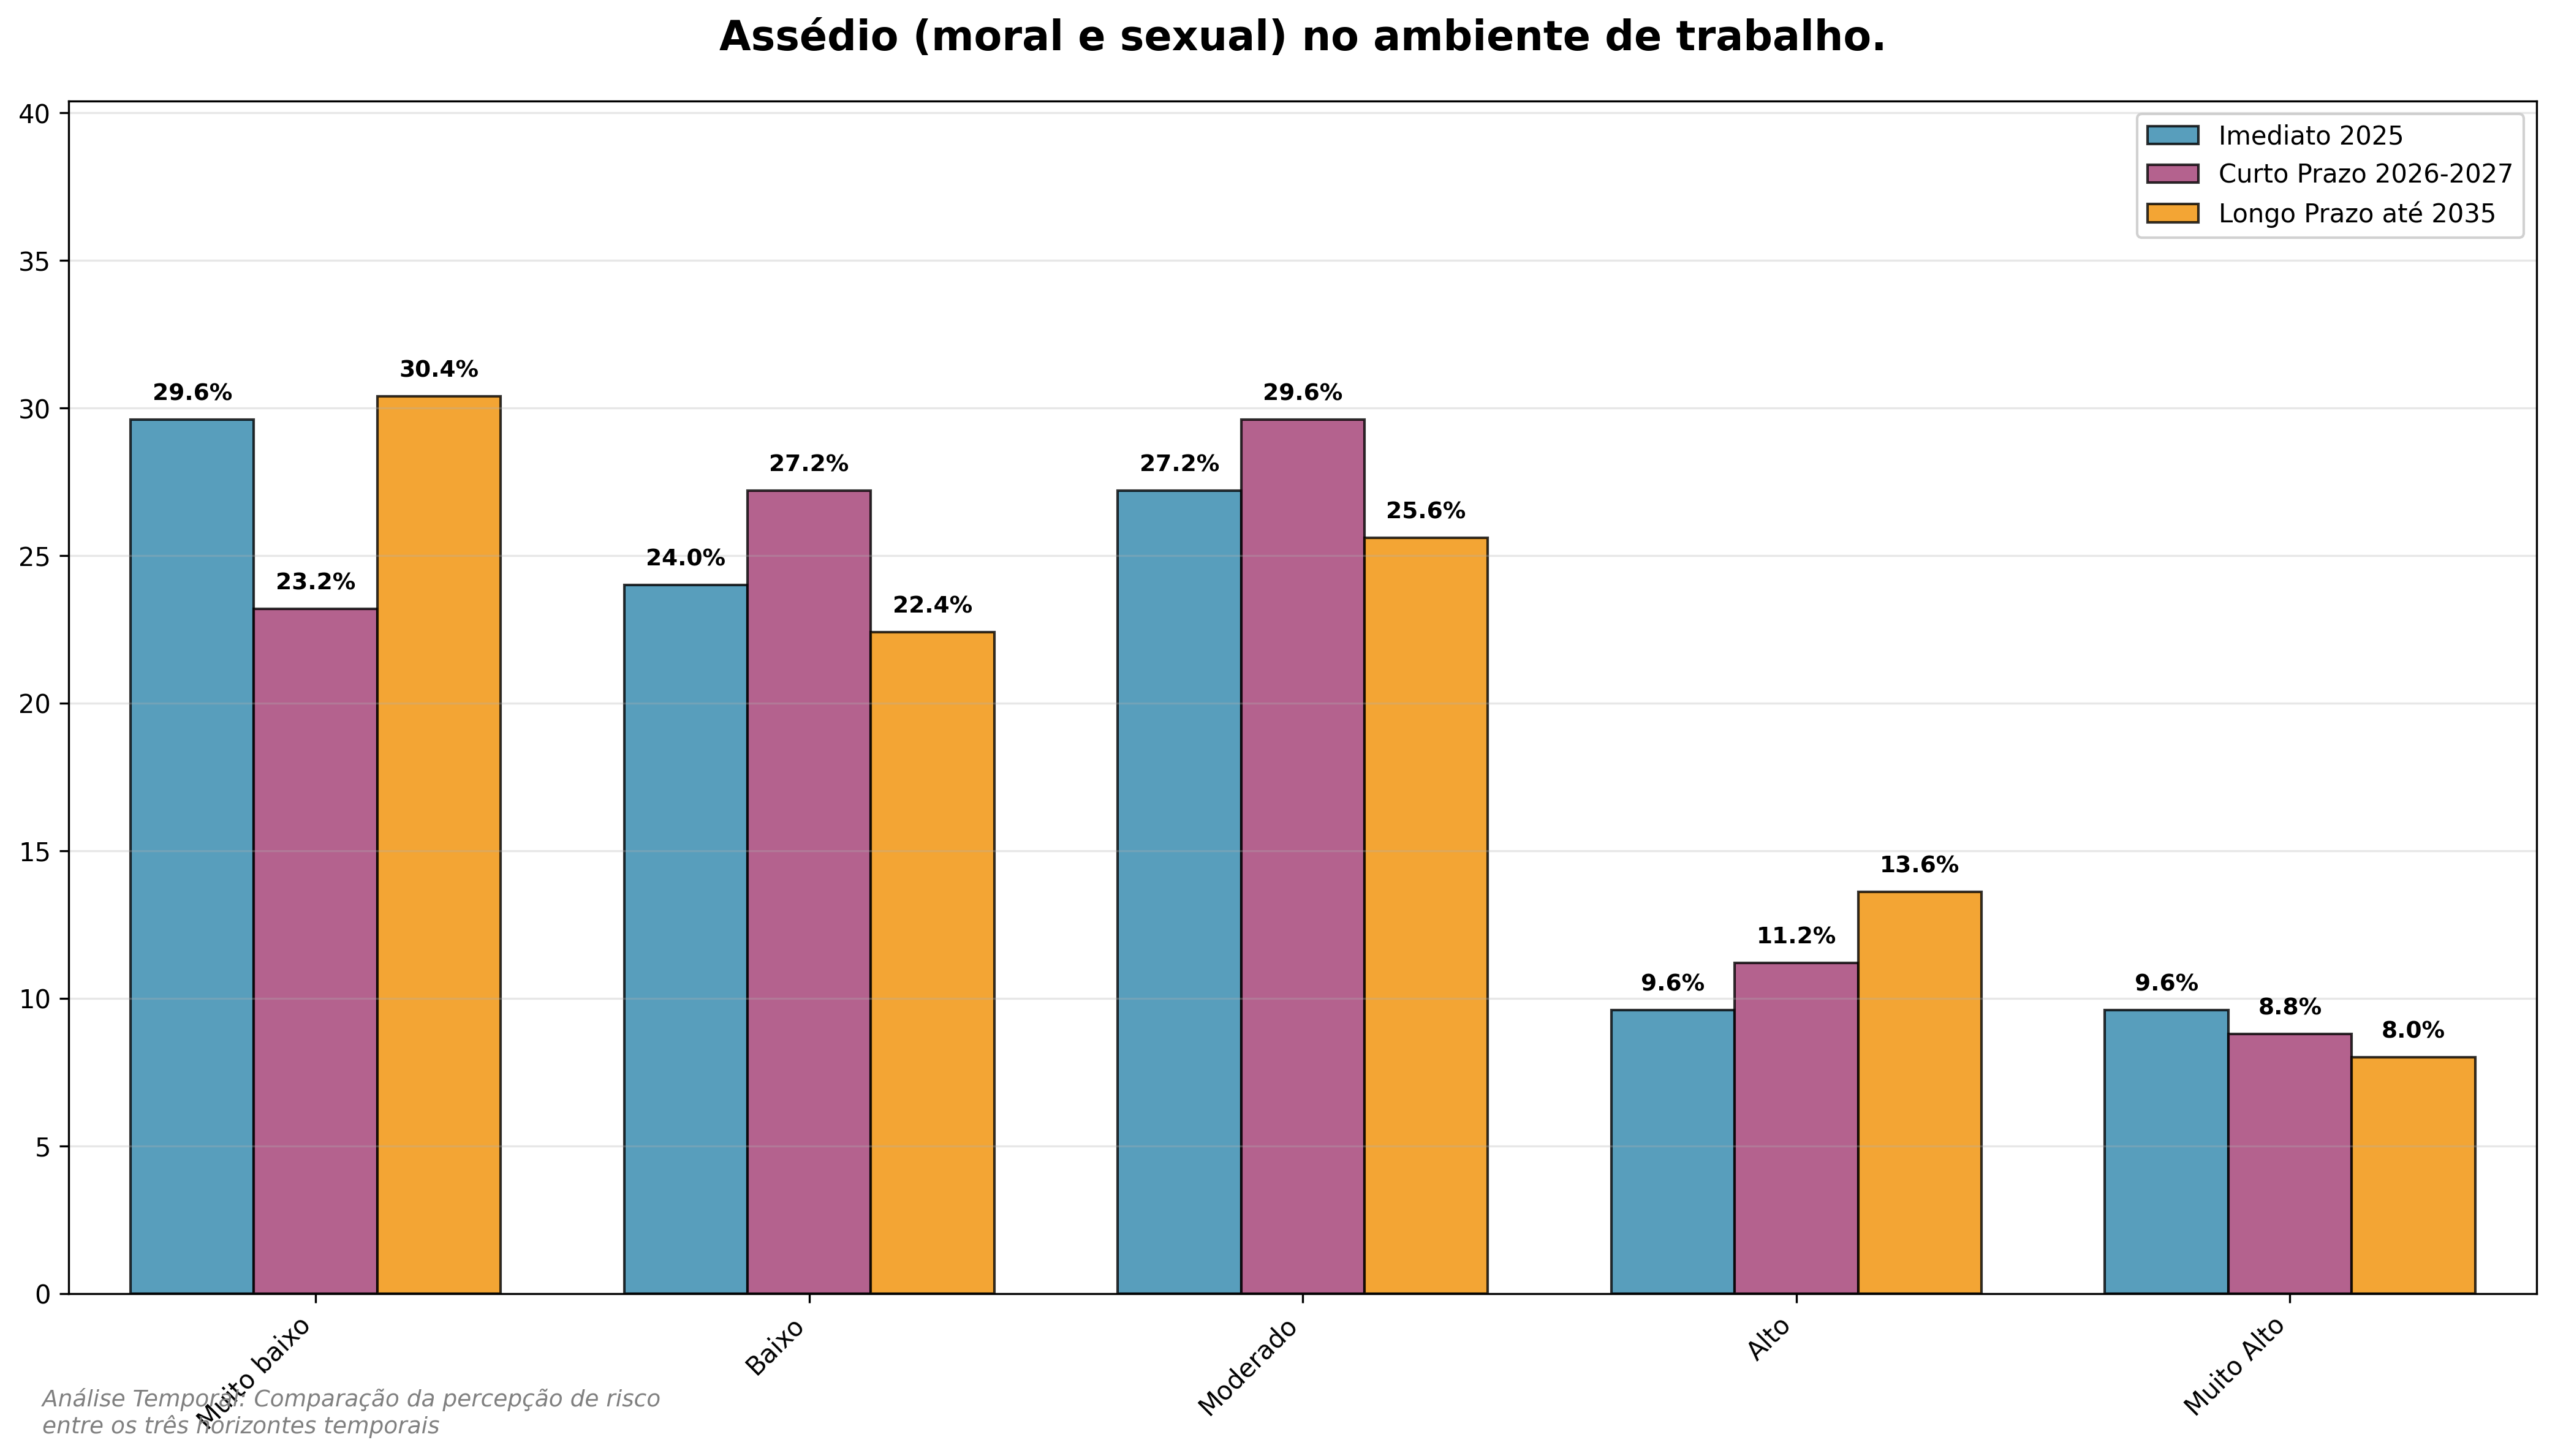
\includegraphics[keepaspectratio]{assets/social/grafico_agrupado_4_11_temporal.png}}

\begin{tcolorbox}[enhanced jigsaw, titlerule=0mm, colback=white, title=\textcolor{quarto-callout-note-color}{\faInfo}\hspace{0.5em}{Destaque}, opacityback=0, colbacktitle=quarto-callout-note-color!10!white, leftrule=.75mm, left=2mm, colframe=quarto-callout-note-color-frame, bottomrule=.15mm, bottomtitle=1mm, breakable, toprule=.15mm, toptitle=1mm, opacitybacktitle=0.6, arc=.35mm, coltitle=black, rightrule=.15mm]

\textbf{Evolução da Percepção de Risco:}

- \textbf{Tendência de crescimento moderado}: Preocupação gradual com
ambiente de trabalho

- \textbf{Mediana}: Mantém-se em 2.0 em todos os períodos - risco
controlado

- \textbf{Risco Alto (níveis 4-5)}: Cresce de 19\% (2025) para 22\%
(2035) - aumento de 12\%

- \textbf{Risco Baixo (níveis 1-2)}: Mantém-se elevado em 64\        (2025)
para 61\                                                             (2035)

\textbf{Contexto Detalhado por Período:}

\textbf{Período Imediato 2025:} Devido ao assédio moral e sexual no
ambiente de trabalho, poderá acontecer altos índices de denúncias,
rotatividade e conflitos trabalhistas, o que poderá levar a ações
judiciais, afastamentos e deterioração do clima organizacional
impactando o bem-estar das equipes e a atratividade do ambiente de
trabalho. No período imediato 2025, 19\% das respostas permanecem nos
níveis 4-5 e a mediana em 2 indica um nível controlado sob vigilância.

\textbf{Período Curto Prazo 2026-2027:} A preocupação com assédio se
mantém controlada, atingindo 20\% das respostas nos níveis 4-5 com
mediana em 2, configurando um nível controlado sob vigilância.

\textbf{Período Longo Prazo até 2035:} A situação permanece controlada,
com 22\% das respostas nos níveis 4-5 e mediana em 2, indicando um risco
controlado sob vigilância.

\textbf{Implicações Estratégicas:} Apesar do crescimento moderado, o
assédio requer políticas preventivas robustas, canais de denúncia
eficazes e cultura organizacional inclusiva. A manutenção do risco em
nível controlado indica eficácia das medidas preventivas, mas exige
vigilância contínua.

\end{tcolorbox}

\subsection{Desigualdades raciais/étnicas e de
gênero}\label{desigualdades-raciaisuxe9tnicas-e-de-guxeanero}

O gr?fico a seguir apresenta a evolu??o temporal do risco Desigualdades
raciais/étnicas e de gênero.
\pandocbounded{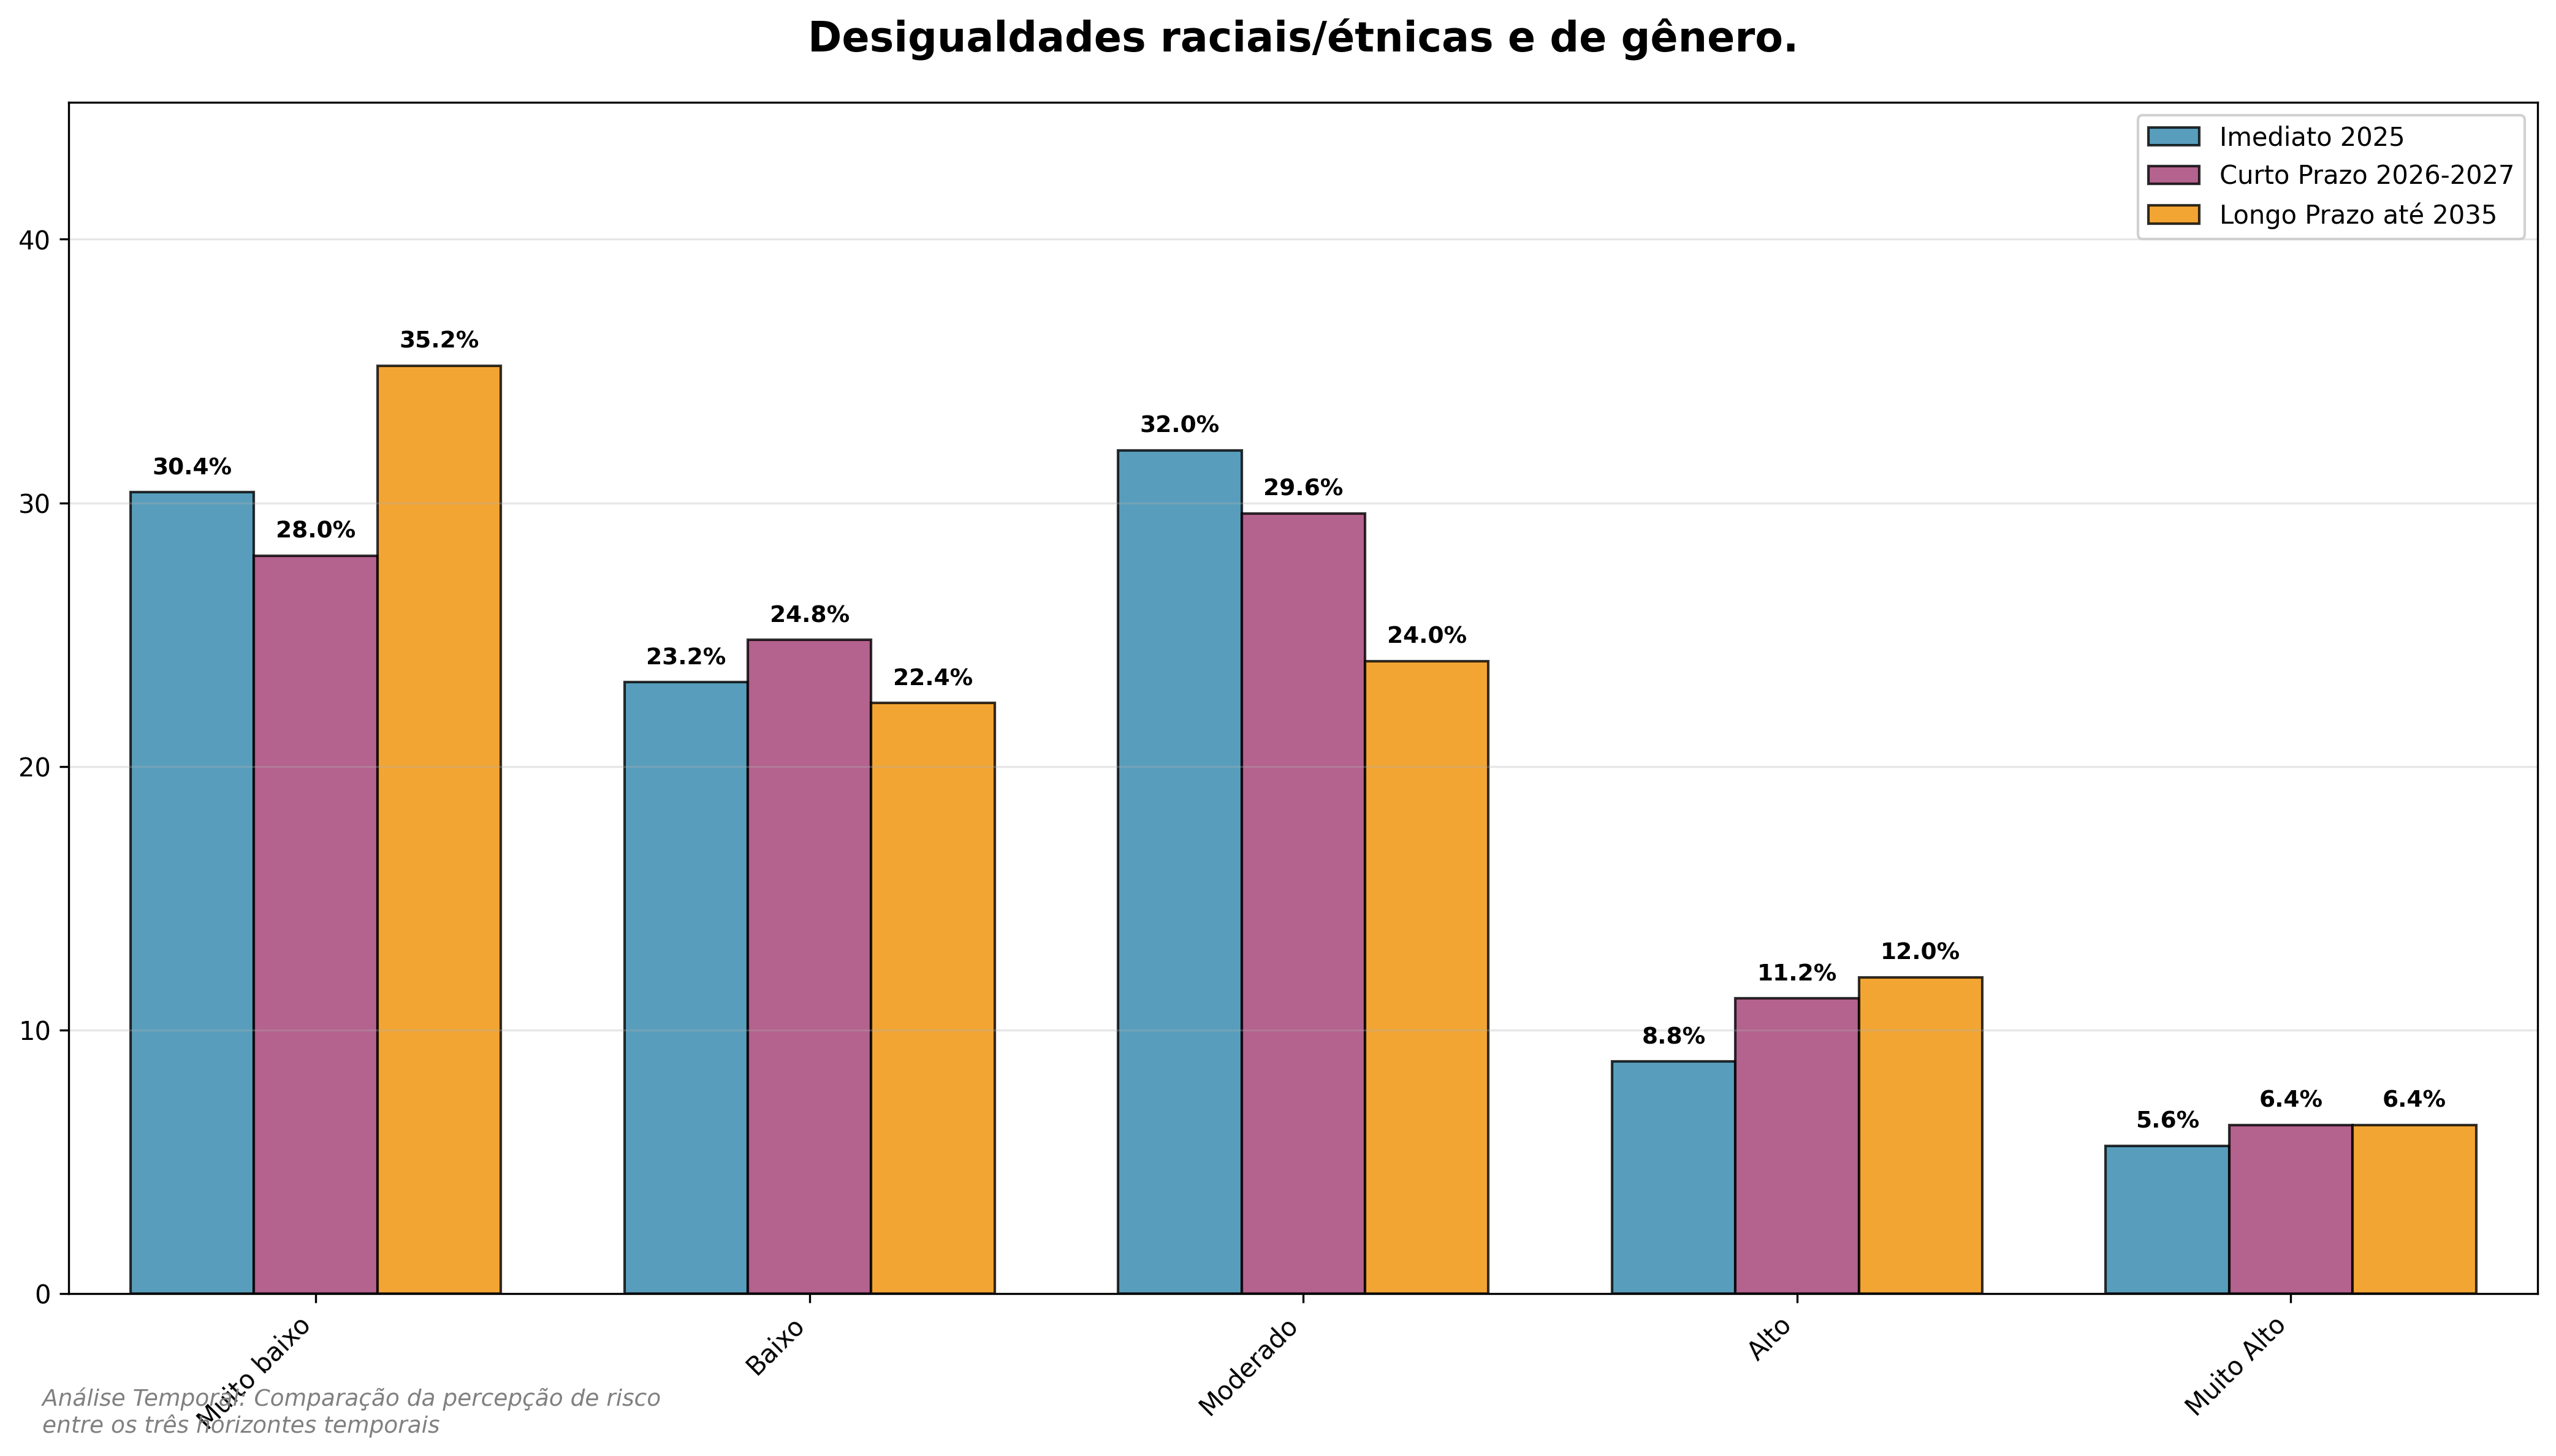
\includegraphics[keepaspectratio]{assets/social/grafico_agrupado_4_12_temporal.png}}

\begin{tcolorbox}[enhanced jigsaw, titlerule=0mm, colback=white, title=\textcolor{quarto-callout-note-color}{\faInfo}\hspace{0.5em}{Destaque}, opacityback=0, colbacktitle=quarto-callout-note-color!10!white, leftrule=.75mm, left=2mm, colframe=quarto-callout-note-color-frame, bottomrule=.15mm, bottomtitle=1mm, breakable, toprule=.15mm, toptitle=1mm, opacitybacktitle=0.6, arc=.35mm, coltitle=black, rightrule=.15mm]

\textbf{Evolução da Percepção de Risco:}

- \textbf{Tendência de crescimento leve}: Preocupação crescente mas
controlada

- \textbf{Mediana}: Mantém-se em 2.0 em todos os períodos - risco
controlado

- \textbf{Risco Alto (níveis 4-5)}: Cresce de 14\% (2025) para 18\%
(2035) - aumento de 28\%

- \textbf{Risco Baixo (níveis 1-2)}: Mantém-se elevado em 68\        (2025)
para 65\                                                             (2035)

\textbf{Contexto Detalhado por Período:}

\textbf{Período Imediato 2025:} Devido às desigualdades raciais, étnicas
e de gênero, poderá acontecer processos seletivos excludentes,
desigualdade salarial e baixa representatividade, o que poderá levar a
reputação negativa, sanções regulatórias e engajamento limitado
impactando a agenda de diversidade, equidade e inclusão do setor. No
período imediato 2025, 14\% das respostas permanecem nos níveis 4-5 e a
mediana em 2 indica um nível controlado sob vigilância.

\textbf{Período Curto Prazo 2026-2027:} A preocupação com desigualdades
se mantém controlada, atingindo 18\% das respostas nos níveis 4-5 com
mediana em 2, configurando um nível controlado sob vigilância.

\textbf{Período Longo Prazo até 2035:} A situação permanece controlada,
com 18\% das respostas nos níveis 4-5 e mediana em 2, indicando um risco
controlado sob vigilância.

\textbf{Implicações Estratégicas:} Desigualdades requerem programas de
diversidade e inclusão, metas de representatividade e auditorias de
equidade para promover ambiente mais justo. A manutenção do risco em
nível controlado indica progresso nas políticas de inclusão, mas exige
monitoramento contínuo.

\end{tcolorbox}

\subsection{Falta de participação
social}\label{falta-de-participauxe7uxe3o-social}

O gr?fico a seguir apresenta a evolu??o temporal do risco Falta de
participação social.
\pandocbounded{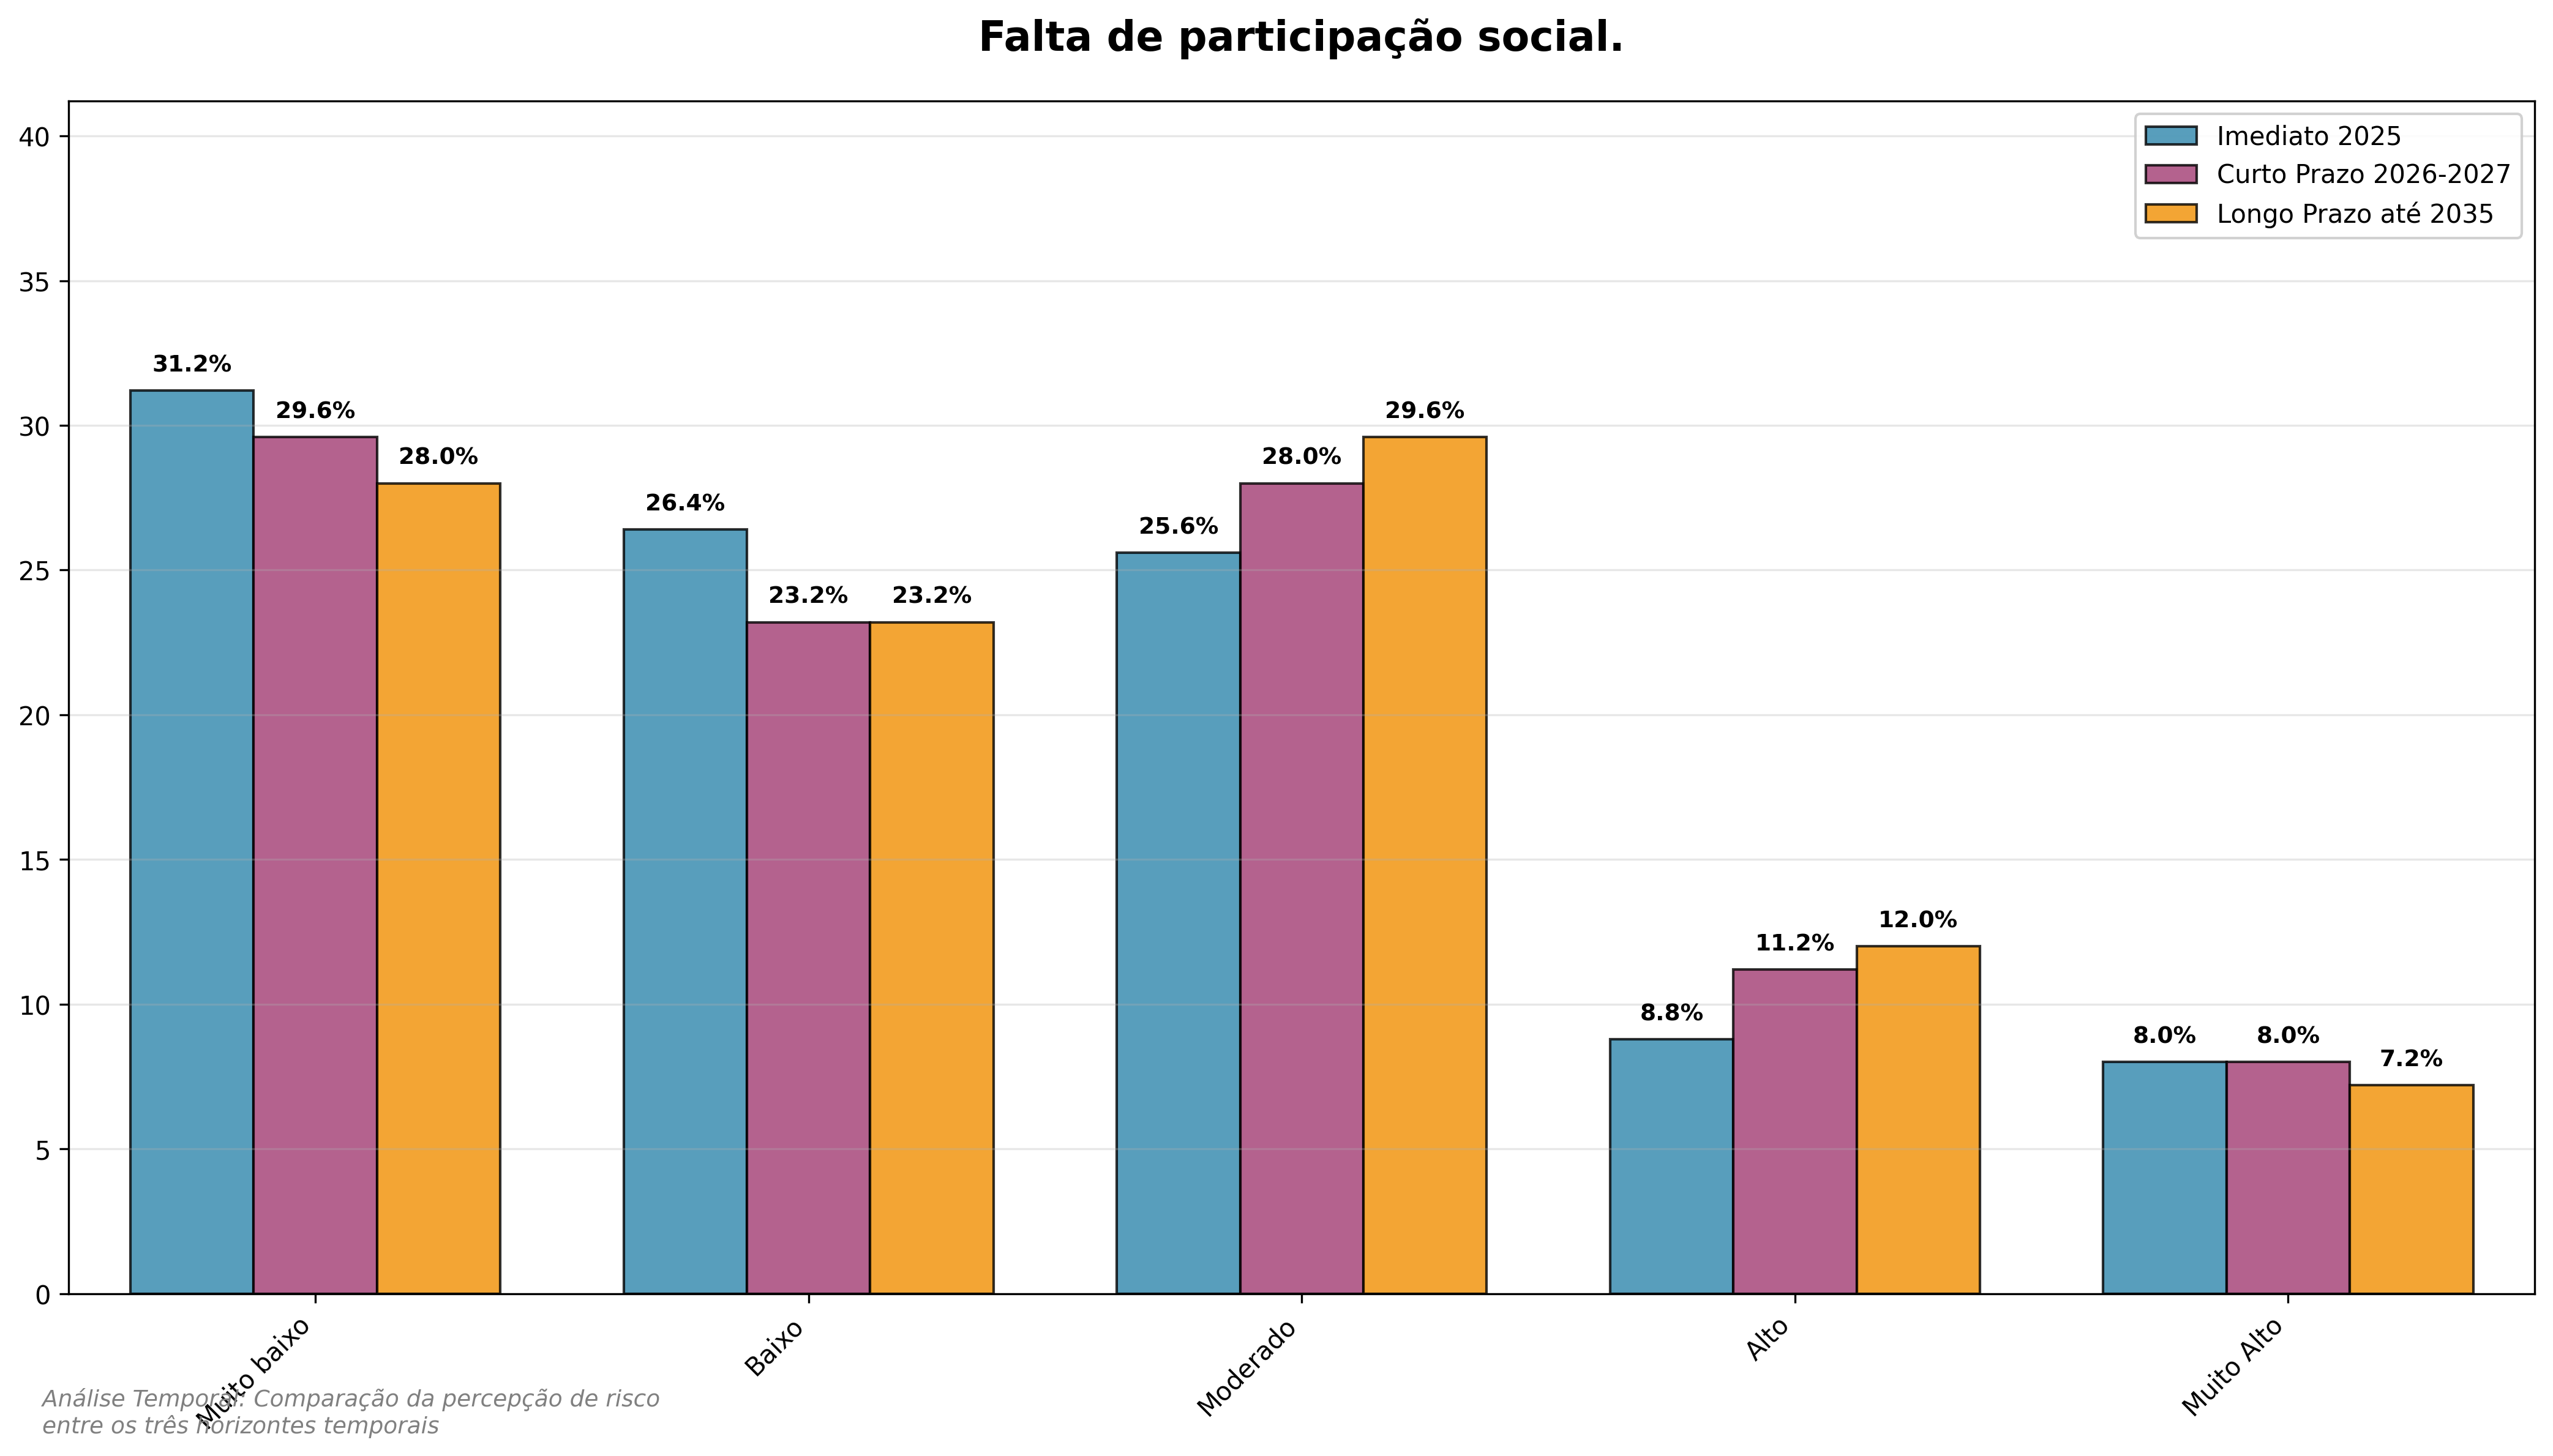
\includegraphics[keepaspectratio]{assets/social/grafico_agrupado_4_13_temporal.png}}

\begin{tcolorbox}[enhanced jigsaw, titlerule=0mm, colback=white, title=\textcolor{quarto-callout-note-color}{\faInfo}\hspace{0.5em}{Destaque}, opacityback=0, colbacktitle=quarto-callout-note-color!10!white, leftrule=.75mm, left=2mm, colframe=quarto-callout-note-color-frame, bottomrule=.15mm, bottomtitle=1mm, breakable, toprule=.15mm, toptitle=1mm, opacitybacktitle=0.6, arc=.35mm, coltitle=black, rightrule=.15mm]

\textbf{Evolução da Percepção de Risco:}

- \textbf{Tendência de crescimento moderado}: Preocupação gradual com
engajamento

- \textbf{Mediana}: Mantém-se em 2.0 em todos os períodos - risco
controlado

- \textbf{Risco Alto (níveis 4-5)}: Cresce de 17\% (2025) para 19\%
(2035) - aumento de 14\%

- \textbf{Risco Baixo (níveis 1-2)}: Mantém-se elevado em 65\        (2025)
para 64\                                                             (2035)

\textbf{Contexto Detalhado por Período:}

\textbf{Período Imediato 2025:} Devido à falta de participação social,
poderá acontecer redução de canais de diálogo e aumento de conflitos com
comunidades, o que poderá levar a protestos, judicializações e atraso em
obras ou licenças impactando a licença social para operar e a
legitimidade perante stakeholders. No período imediato 2025, 17\% das
respostas permanecem nos níveis 4-5 e a mediana em 2 indica um nível
controlado sob vigilância.

\textbf{Período Curto Prazo 2026-2027:} A preocupação com participação
social se mantém controlada, atingindo 19\% das respostas nos níveis 4-5
com mediana em 2, configurando um nível controlado sob vigilância.

\textbf{Período Longo Prazo até 2035:} A situação permanece controlada,
com 19\% das respostas nos níveis 4-5 e mediana em 2, indicando um risco
controlado sob vigilância.

\textbf{Implicações Estratégicas:} Participação social exige canais de
diálogo permanentes, consultas públicas e transparência para construir
licença social e legitimidade. A manutenção do risco em nível controlado
indica eficácia dos mecanismos de engajamento, mas requer fortalecimento
contínuo.

\end{tcolorbox}

\subsection{Maior uso de tecnologias (IA, mecanização,
robotização)}\label{maior-uso-de-tecnologias-ia-mecanizauxe7uxe3o-robotizauxe7uxe3o}

O gr?fico a seguir apresenta a evolu??o temporal do risco Maior uso de
tecnologias (IA, mecanização, robotização).
\pandocbounded{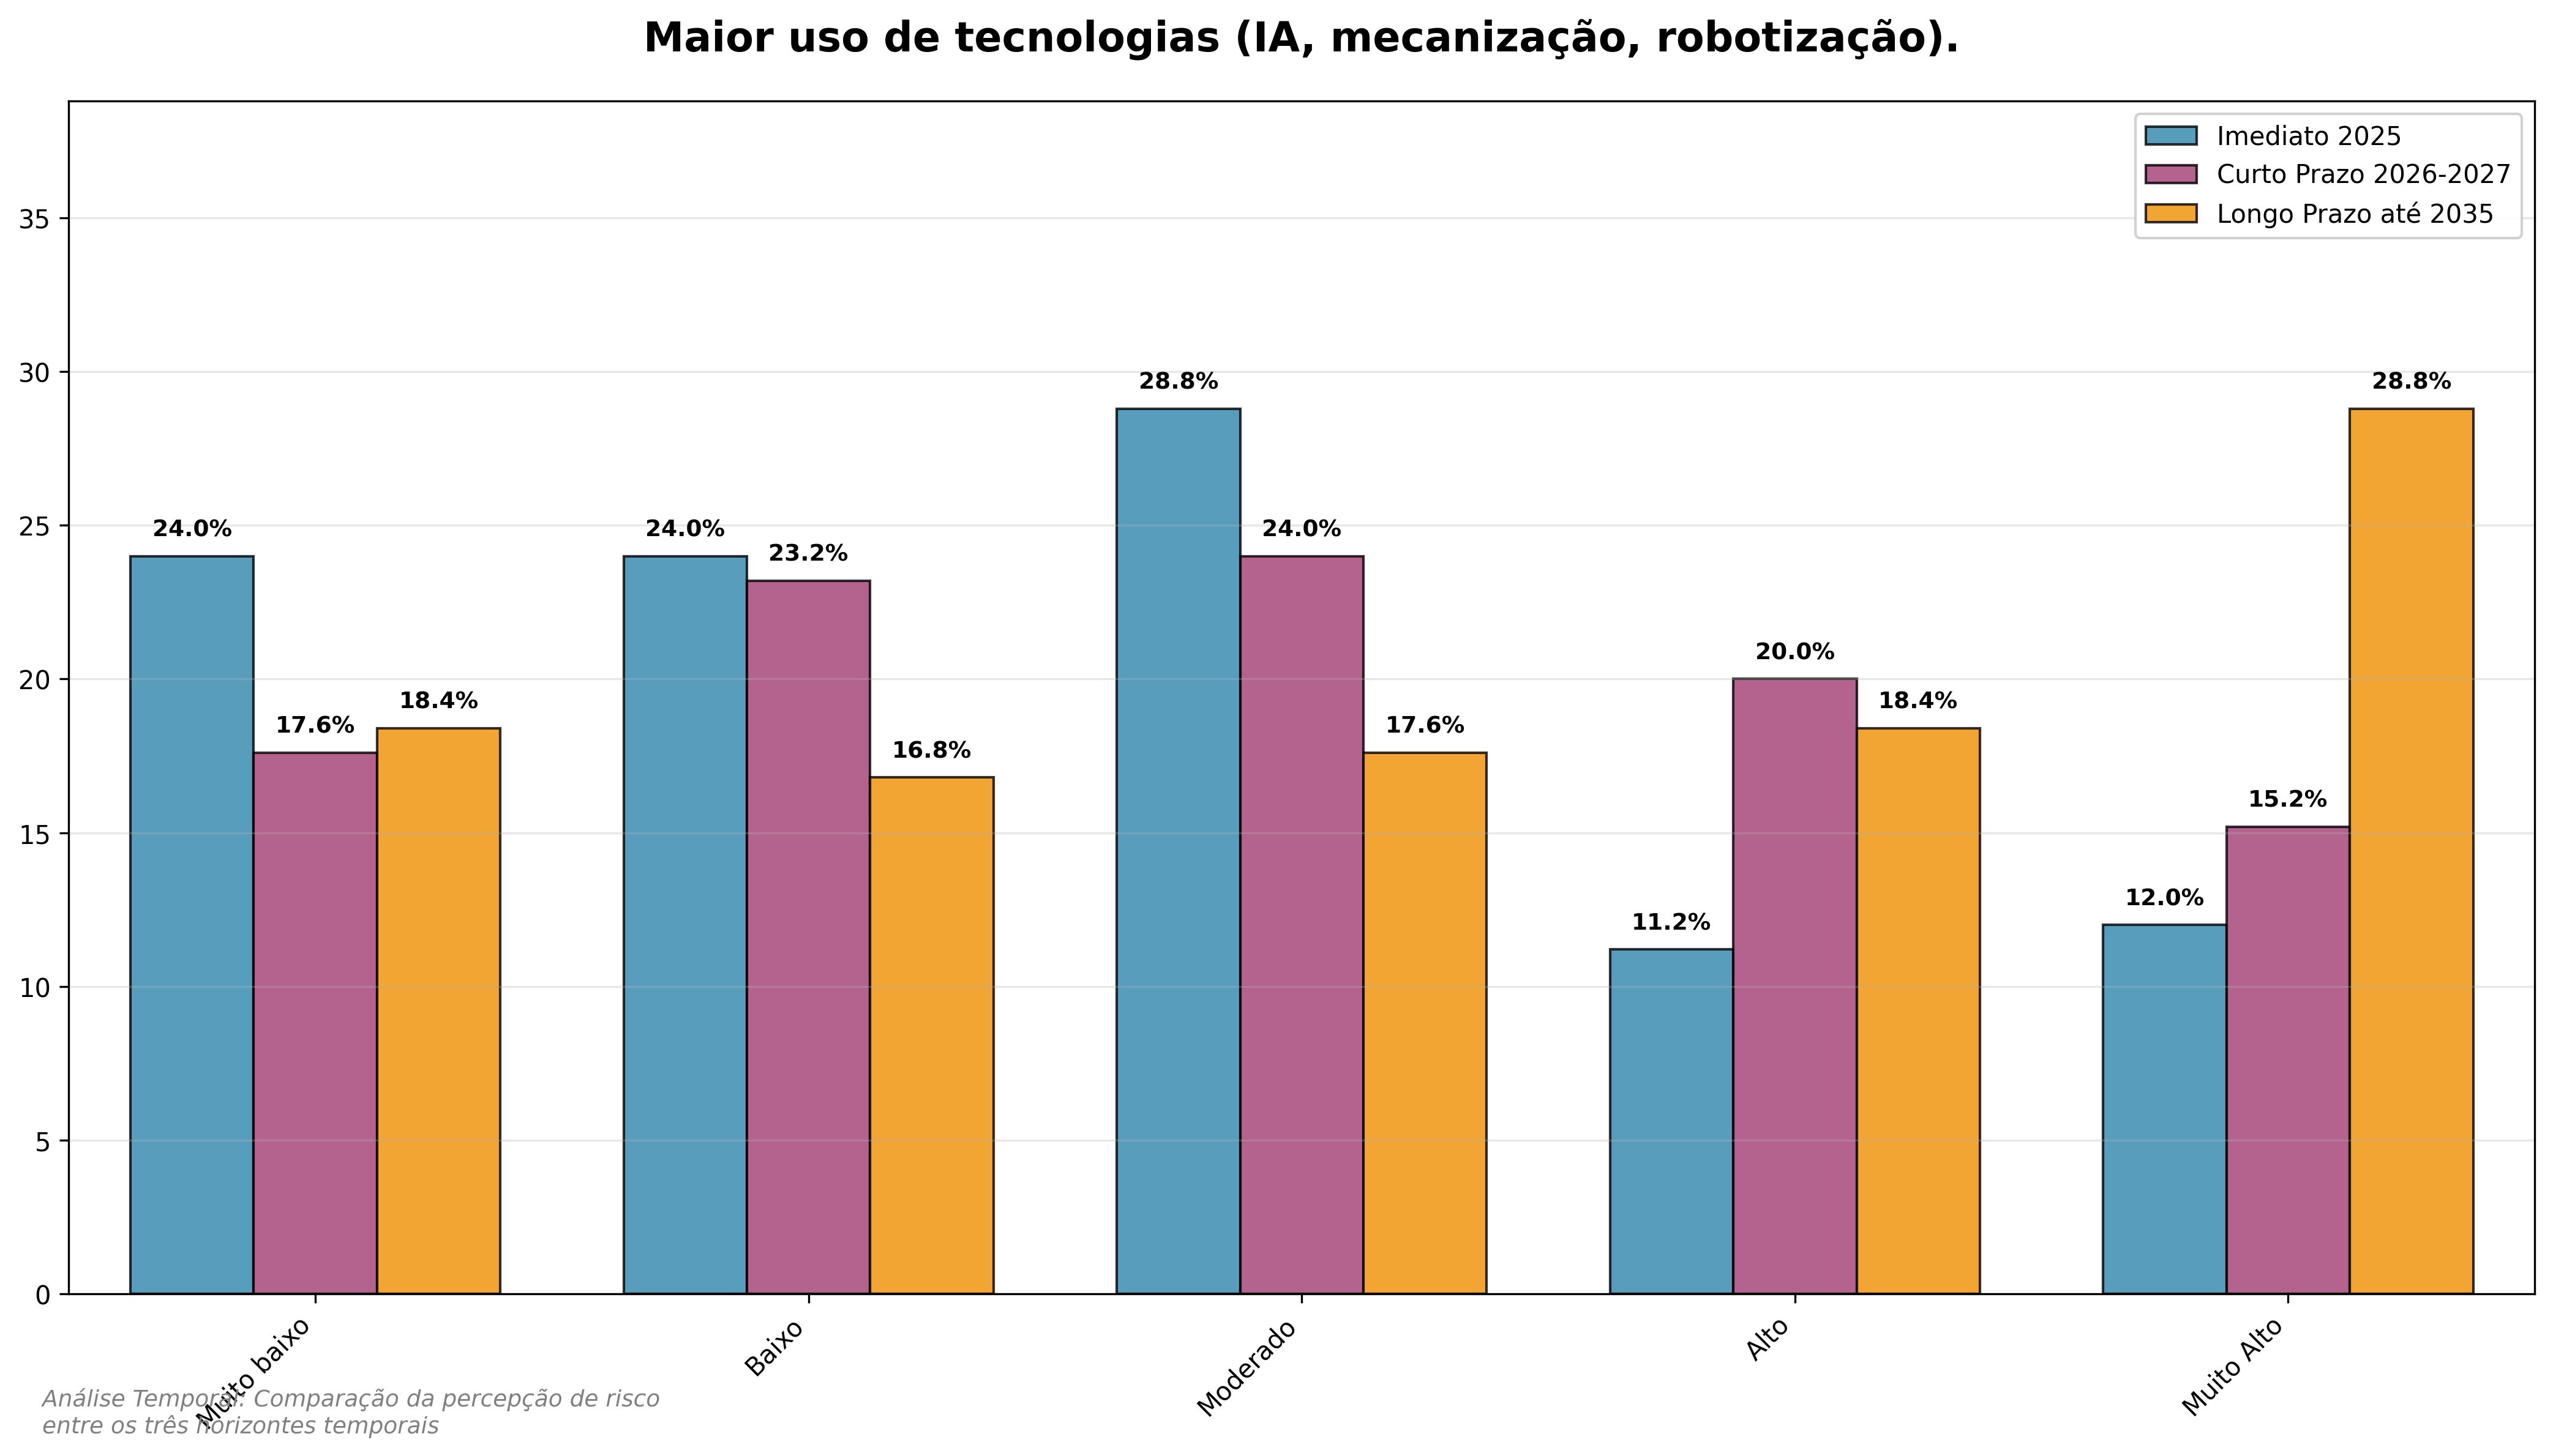
\includegraphics[keepaspectratio]{assets/social/grafico_agrupado_4_14_temporal.png}}

\begin{tcolorbox}[enhanced jigsaw, titlerule=0mm, colback=white, title=\textcolor{quarto-callout-note-color}{\faInfo}\hspace{0.5em}{Destaque}, opacityback=0, colbacktitle=quarto-callout-note-color!10!white, leftrule=.75mm, left=2mm, colframe=quarto-callout-note-color-frame, bottomrule=.15mm, bottomtitle=1mm, breakable, toprule=.15mm, toptitle=1mm, opacitybacktitle=0.6, arc=.35mm, coltitle=black, rightrule=.15mm]

\textbf{Evolução da Percepção de Risco:}

- \textbf{Tendência de crescimento exponencial}: Preocupação crescente
com transformação digital

- \textbf{Mediana}: Mantém-se em 3.0 em todos os períodos - risco
elevado persistente

- \textbf{Risco Alto (níveis 4-5)}: Cresce de 23\% (2025) para 47\%
(2035) - aumento de 103\%

- \textbf{Risco Baixo (níveis 1-2)}: Redução de 37\% (2025) para 20\%
(2035)

\textbf{Contexto Detalhado por Período:}

\textbf{Período Imediato 2025:} Devido ao maior uso de tecnologias como
IA, mecanização e robotização, poderá acontecer erros de automação,
obsolescência de processos e exposição a ciberataques, o que poderá
levar a interrupções operacionais, custos adicionais e risco à
competitividade impactando a modernização tecnológica segura e a
produtividade dos terminais. No período imediato 2025, 23\% das
respostas permanecem nos níveis 4-5 e a mediana em 3 indica um nível
moderado com tendência de crescimento.

\textbf{Período Curto Prazo 2026-2027:} A preocupação com tecnologias se
intensifica, atingindo 35\% das respostas nos níveis 4-5 com mediana em
3, configurando um nível elevado que demanda planos de ação priorizados.

\textbf{Período Longo Prazo até 2035:} A situação se torna crítica, com
47\% das respostas nos níveis 4-5 e mediana em 3, indicando um patamar
crítico que requer medidas imediatas.

\textbf{Implicações Estratégicas:} A transformação tecnológica
representa o risco de maior crescimento, exigindo investimentos em
cibersegurança, treinamento digital e governança de IA para mitigar
riscos. A evolução de moderado para crítico indica necessidade de
planejamento estratégico robusto para transição digital segura.

\end{tcolorbox}

\subsection{Ausência do Estado junto às populações próximas aos
portos}\label{ausuxeancia-do-estado-junto-uxe0s-populauxe7uxf5es-pruxf3ximas-aos-portos}

O gr?fico a seguir apresenta a evolu??o temporal do risco Ausência do
Estado junto às populações próximas aos portos.
\pandocbounded{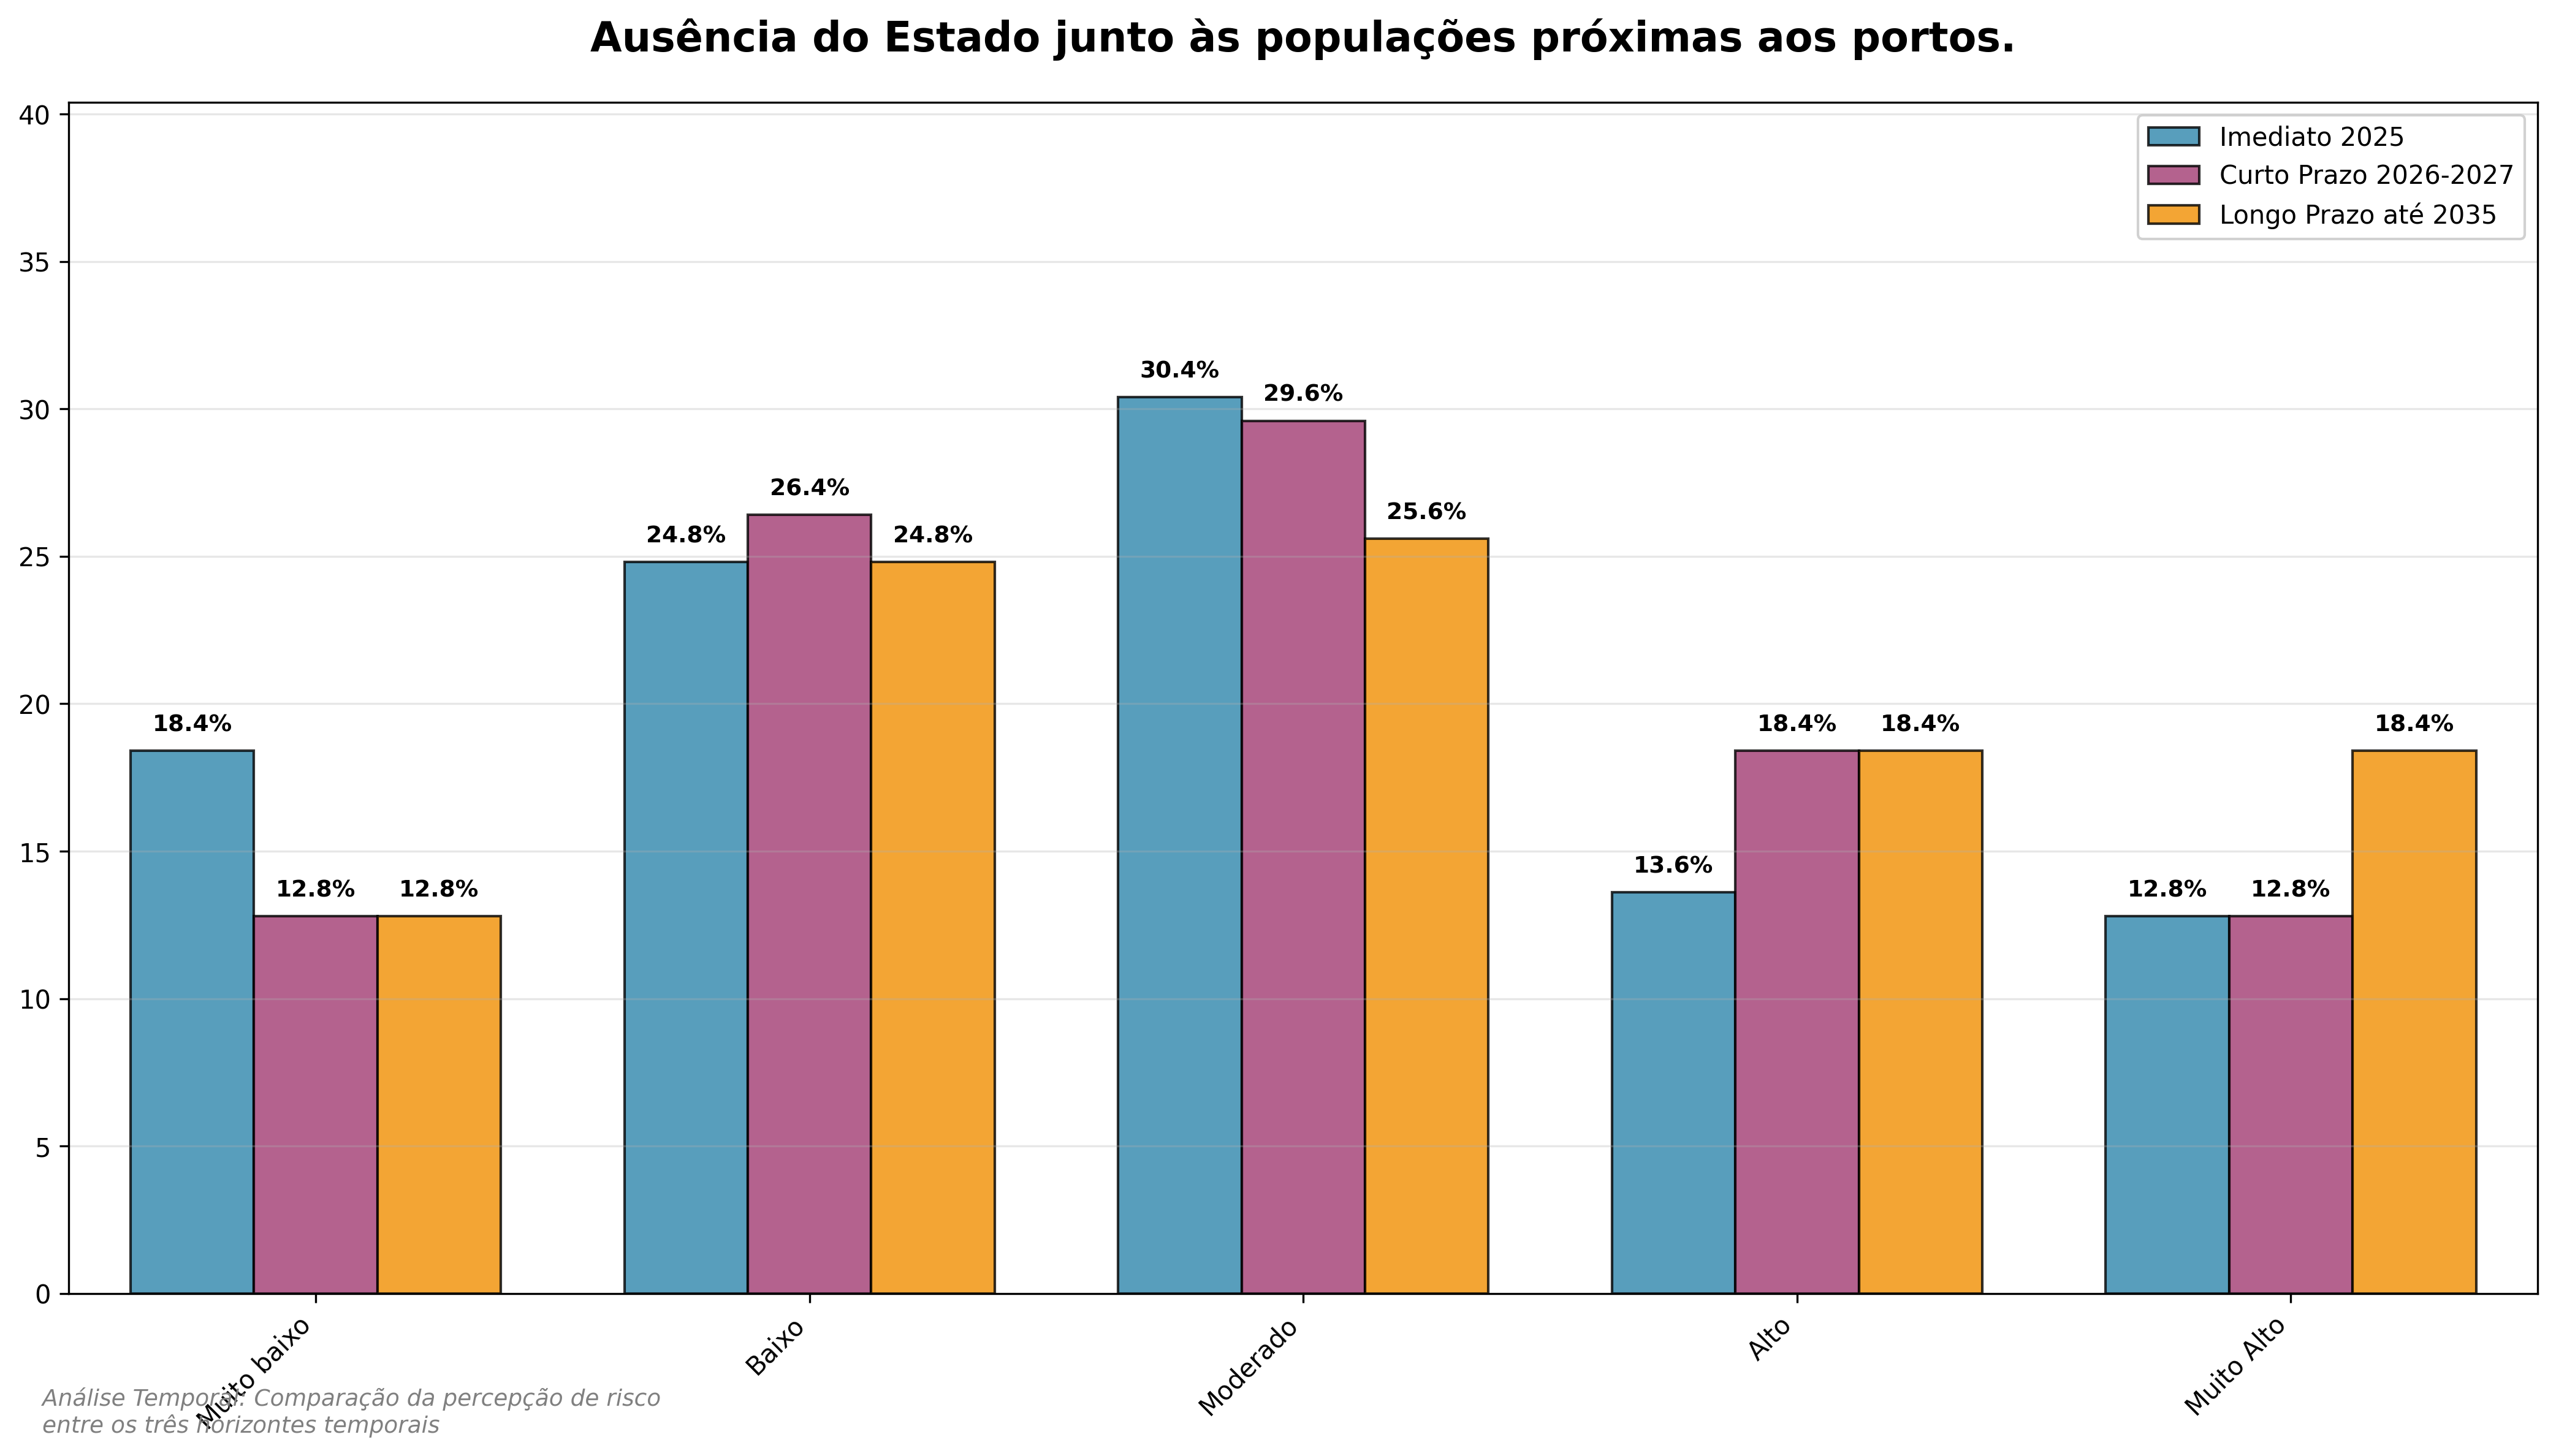
\includegraphics[keepaspectratio]{assets/social/grafico_agrupado_4_15_temporal.png}}

\begin{tcolorbox}[enhanced jigsaw, titlerule=0mm, colback=white, title=\textcolor{quarto-callout-note-color}{\faInfo}\hspace{0.5em}{Destaque}, opacityback=0, colbacktitle=quarto-callout-note-color!10!white, leftrule=.75mm, left=2mm, colframe=quarto-callout-note-color-frame, bottomrule=.15mm, bottomtitle=1mm, breakable, toprule=.15mm, toptitle=1mm, opacitybacktitle=0.6, arc=.35mm, coltitle=black, rightrule=.15mm]

\textbf{Evolução da Percepção de Risco:}

- \textbf{Tendência de crescimento significativo}: Preocupação crescente
com vácuo institucional

- \textbf{Mediana}: Mantém-se em 3.0 em todos os períodos

- \textbf{Risco Alto (níveis 4-5)}: Cresce de 26\% (2025) para 37\%
(2035) - aumento de 39\%

- \textbf{Risco Baixo (níveis 1-2)}: Redução de 40\% (2025) para 32\%
(2035)

\textbf{Contexto Detalhado por Período:}

\textbf{Período Imediato 2025:} Devido à ausência do Estado junto às
populações próximas aos portos, poderá acontecer vazios de políticas
públicas e carência de serviços básicos para as comunidades portuárias,
o que poderá levar a pressão social, aumento de vulnerabilidades e
escalada de conflitos impactando a harmonia comunitária e a continuidade
das operações. No período imediato 2025, 26\% das respostas permanecem
nos níveis 4-5 e a mediana em 3 indica um nível moderado com tendência
de crescimento.

\textbf{Período Curto Prazo 2026-2027:} A preocupação com ausência
estatal se intensifica, atingindo 31\% das respostas nos níveis 4-5 com
mediana em 3, configurando um nível elevado que demanda planos de ação
priorizados.

\textbf{Período Longo Prazo até 2035:} A situação se torna mais crítica,
com 37\% das respostas nos níveis 4-5 e mediana em 3, indicando um risco
elevado e persistente que requer investimentos contínuos.

\textbf{Implicações Estratégicas:} A ausência estatal exige parcerias
público-privadas, investimentos sociais e advocacy para garantir
desenvolvimento sustentável das comunidades portuárias. A evolução de
moderado para elevado indica necessidade de planejamento estratégico
para compensar vácuos institucionais.

\end{tcolorbox}

\section{Análise Temporal
Comparativa}\label{anuxe1lise-temporal-comparativa-3}

A análise comparativa entre os horizontes temporais revela importantes
padrões para a dimensão social, evidenciando a escalada dos riscos
ligados à ausência do Estado, aos serviços essenciais e às
transformações tecnológicas que impactam diretamente as comunidades
portuárias.

\subsection{Tendências
Identificadas}\label{tenduxeancias-identificadas-3}

\begin{itemize}
\tightlist
\item
  \textbf{Riscos Imediatos}: A falta de presença estatal já pressiona as
  áreas portuárias, com 26\% das respostas nos níveis 4-5 e mediana 3,
  indicando necessidade de respostas rápidas para assegurar serviços
  básicos e reduzir tensões comunitárias.
\item
  \textbf{Riscos de Curto Prazo}: Entre 2026 e 2027 o risco alto alcança
  31\% das respostas, refletindo intensificação das vulnerabilidades em
  serviços essenciais e recursos humanos e sinalizando que a capacidade
  institucional atual não acompanhará a demanda crescente.
\item
  \textbf{Riscos de Longo Prazo}: Até 2035 o risco alto sobe para 37\%
  (aumento de 39\% em relação a 2025), impulsionado por tecnologias
  emergentes (+103\% em risco alto), pandemias (+74\%) e direitos
  humanos (+58\%), consolidando tendência estrutural de agravamento sem
  ações coordenadas.
\end{itemize}

\subsection{Insights Estratégicos}\label{insights-estratuxe9gicos}

\begin{enumerate}
\def\labelenumi{\arabic{enumi}.}
\tightlist
\item
  \textbf{Presença Institucional}: Estruturar parcerias público-privadas
  e agendas de advocacy para mitigar o vácuo estatal e assegurar
  continuidade de políticas sociais.
\item
  \textbf{Serviços Essenciais}: Direcionar investimentos para saúde,
  educação, saneamento e mobilidade nas áreas portuárias, reduzindo a
  pressão social que já se manifesta no horizonte imediato.
\item
  \textbf{Capacitação e Trabalho Digno}: Implantar programas de formação
  e retenção de talentos locais para preparar a mão de obra para
  tecnologias emergentes e reduzir vulnerabilidades em direitos humanos.
\item
  \textbf{Resiliência Sanitária e Tecnológica}: Implementar planos de
  contingência para pandemias e protocolos de adoção tecnológica
  responsável, equilibrando inovação com proteção social.
\end{enumerate}

\bookmarksetup{startatroot}

\chapter{Riscos Tecnológicos}\label{riscos-tecnoluxf3gicos-1}

Este capítulo apresenta a análise dos riscos tecnológicos identificados
organizados por horizontes temporais.

\section{Visão Geral dos Riscos
Tecnológicos}\label{visuxe3o-geral-dos-riscos-tecnoluxf3gicos}

Os riscos tecnológicos foram avaliados em três horizontes temporais:

\begin{itemize}
\tightlist
\item
  \textbf{Imediato (2025)}: Riscos que requerem atenção imediata;-
  \textbf{Curto Prazo (2026-2027)}: Riscos emergentes que demandam
  planejamento;- \textbf{Longo Prazo (até 2035)}: Riscos estratégicos
  que requerem visão de futuro. \#\# Panorama do Período Imediato
\end{itemize}

O gr?fico a seguir mostra a distribui??o dos riscos no per?odo imediato.
\pandocbounded{\includegraphics[keepaspectratio]{assets/tecnologicos/grafico_barras_imediato_2025.png}}

\begin{tcolorbox}[enhanced jigsaw, titlerule=0mm, colback=white, title=\textcolor{quarto-callout-note-color}{\faInfo}\hspace{0.5em}{Destaques do período Imediato de 2025}, opacityback=0, colbacktitle=quarto-callout-note-color!10!white, leftrule=.75mm, left=2mm, colframe=quarto-callout-note-color-frame, bottomrule=.15mm, bottomtitle=1mm, breakable, toprule=.15mm, toptitle=1mm, opacitybacktitle=0.6, arc=.35mm, coltitle=black, rightrule=.15mm]

\begin{itemize}
\tightlist
\item
  \textbf{Atraso no processo de digitalização}: 34\% em níveis altos;
\item
  \textbf{Vulnerabilidades em comunicação e IoT}: 33\% em níveis altos;
\item
  \textbf{Consequências indesejáveis de tecnologias}: 20\% em níveis
  altos.
\end{itemize}

\end{tcolorbox}

\section{Análise Temporal da Dimensão
Tecnológica}\label{anuxe1lise-temporal-da-dimensuxe3o-tecnoluxf3gica}

O gr?fico a seguir sintetiza a evolu??o temporal das vari?veis da
dimens?o tecnol?gica.
\pandocbounded{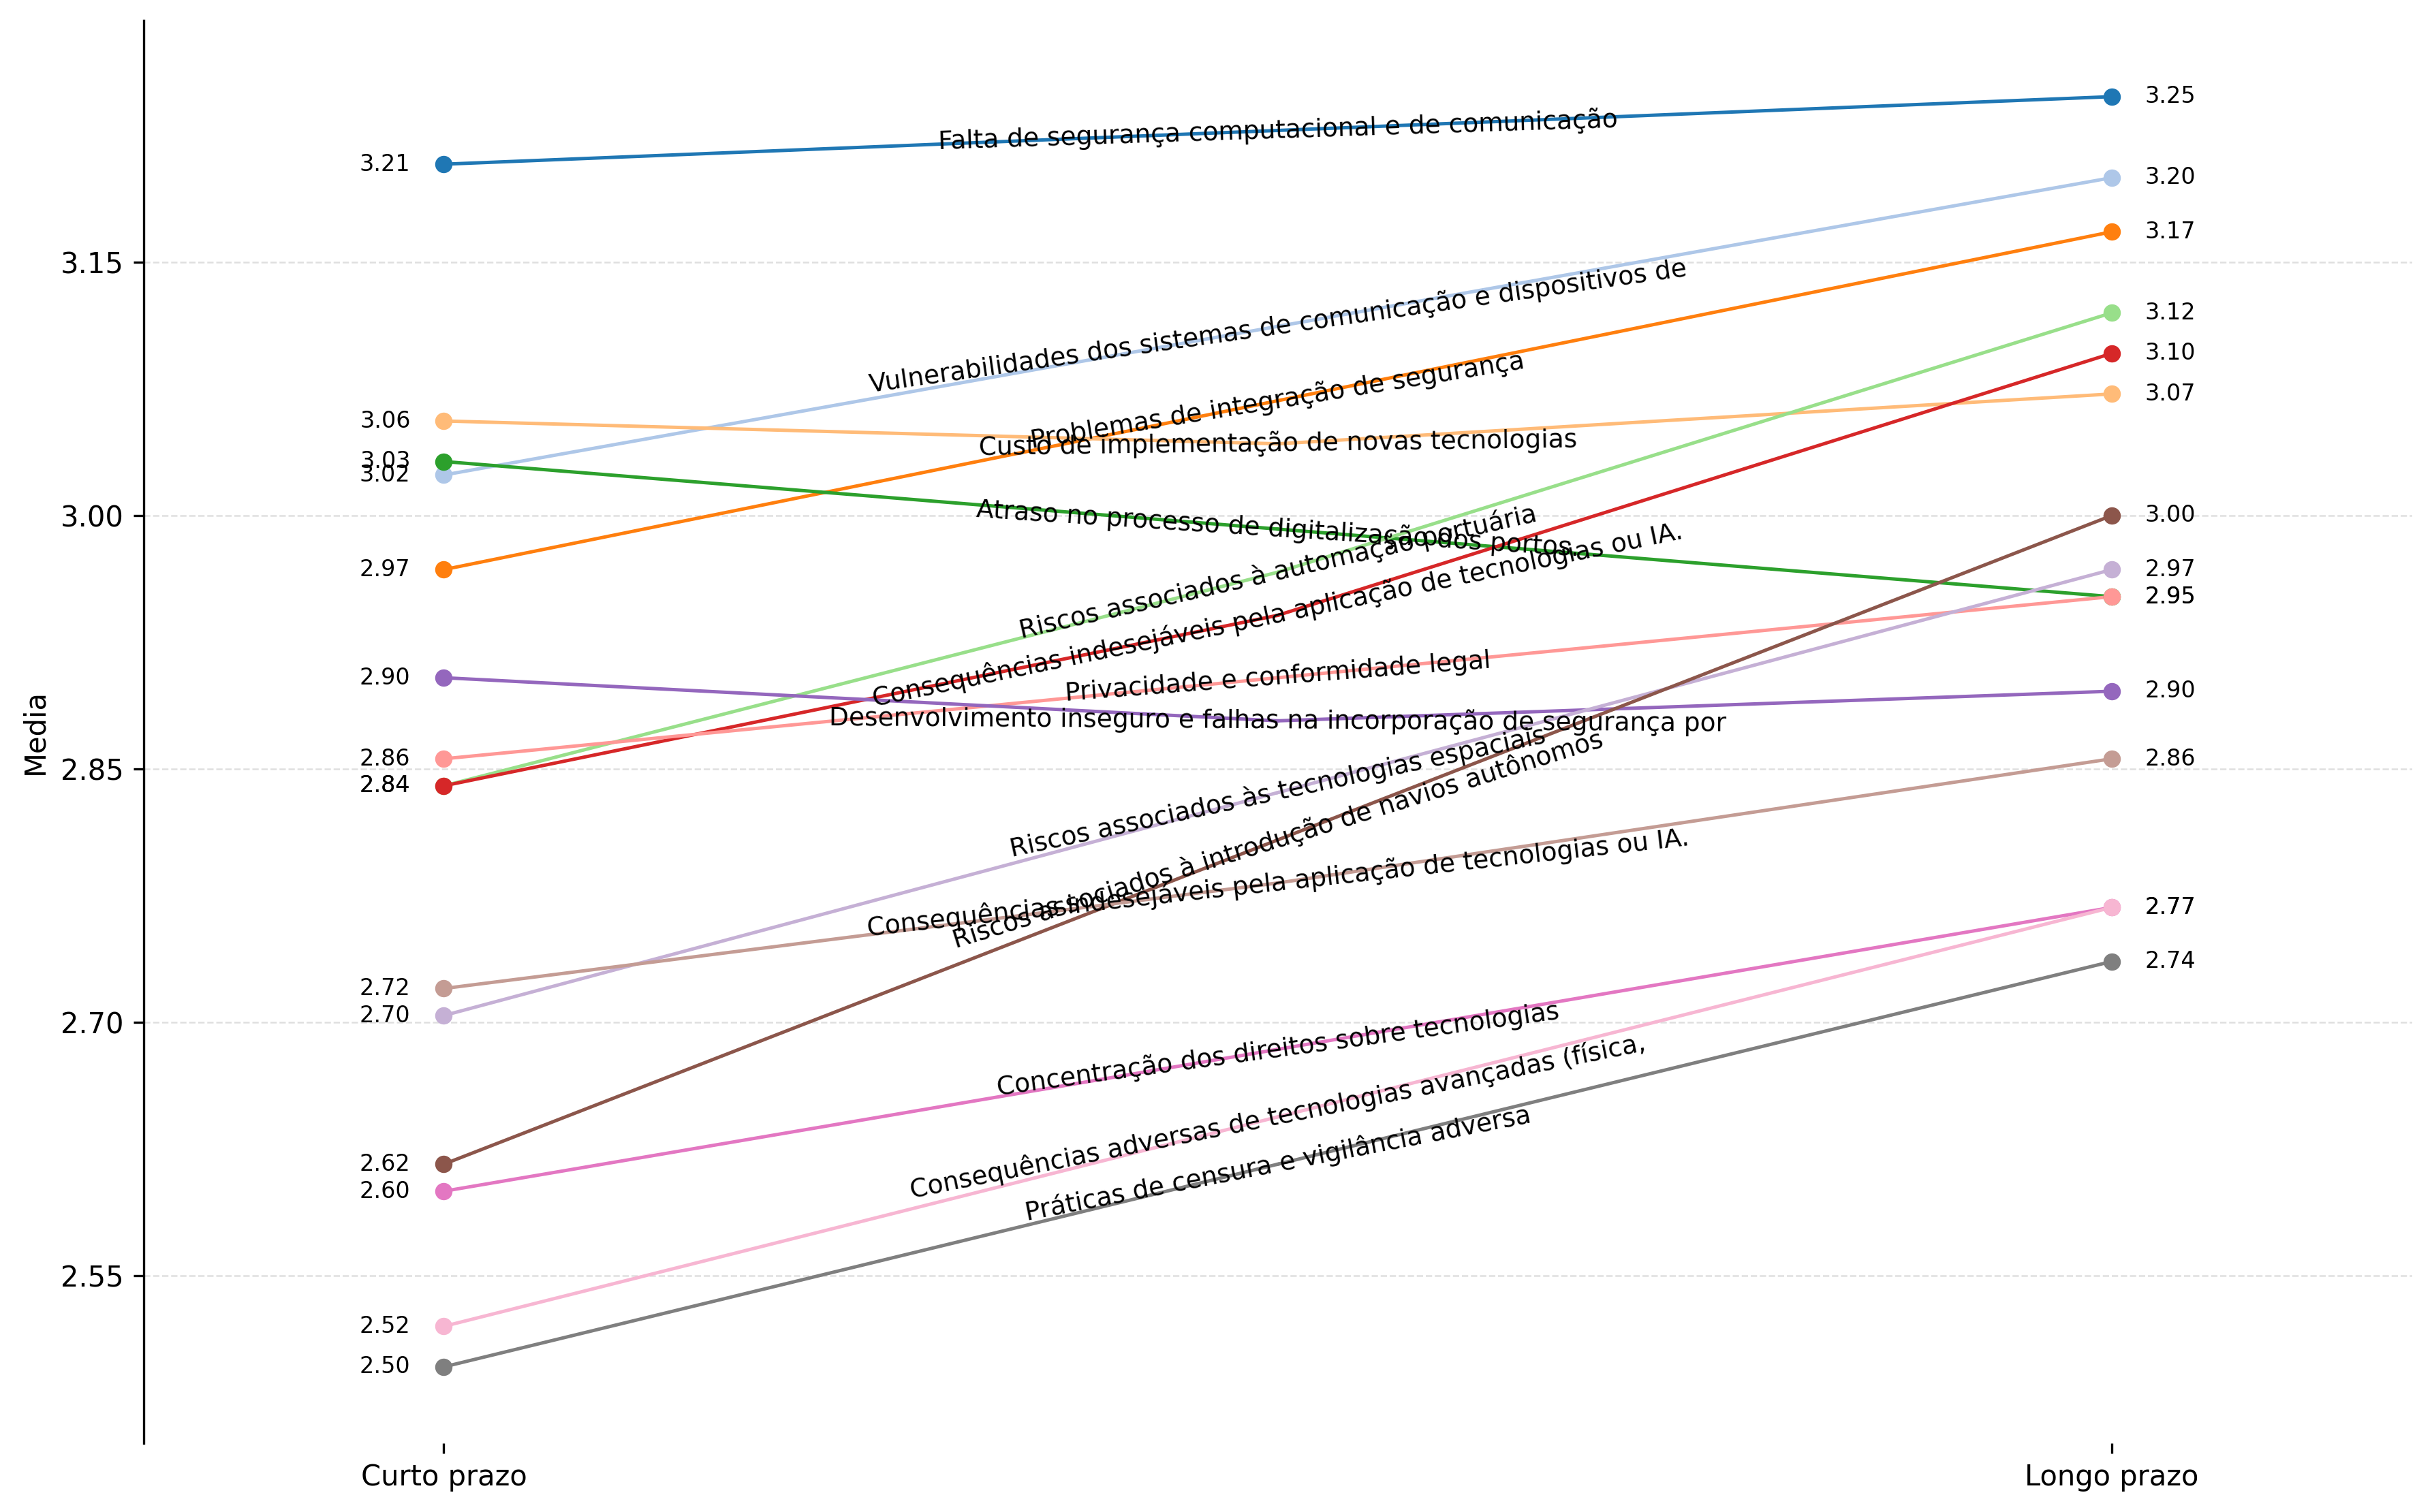
\includegraphics[keepaspectratio]{assets/slopegraphs_por_dimensao/slopegraph_tecnologica.png}}

A dimensão tecnológica apresenta padrões temporais complexos que
refletem tanto os desafios da transformação digital quanto as
oportunidades de inovação no setor portuário.

\subsection{Insights da Análise Temporal
Tecnológica}\label{insights-da-anuxe1lise-temporal-tecnoluxf3gica}

A análise temporal dos riscos tecnológicos revela padrões de evolução
digital e adaptação:

\subsubsection{Piora Tecnológica
Controlada}\label{piora-tecnoluxf3gica-controlada}

\begin{itemize}
\item
  \textbf{Delta médio de +0,20}: Piora moderada em comparação com outras
  dimensões;- \textbf{1 variável com piora crítica (+1.0 ponto)}:
  Ataques cibernéticos e ransomware;- \textbf{Tendência de deterioração
  gradual}: A maioria dos riscos mostra piora progressiva. \#\#\#\#
  Padrões Específicos Identificados
\item
  \textbf{Cibersegurança como Principal Preocupação}: Ataques
  cibernéticos evoluem de mediana 2.0 para 3.0;- \textbf{Desafios de
  Automação}: Falhas em sistemas de automação mantêm-se persistentemente
  altas;- \textbf{Gap de Competências Tecnológicas}: Falta de mão de
  obra qualificada mostra piora consistente. \#\#\#\# Destaques da
  Evolução Temporal
\item
  \textbf{Risco Mais Crítico em 2035}: Falhas em sistemas de automação e
  controle (45\% em risco alto);- \textbf{Maior Crescimento Relativo}:
  Ataques cibernéticos e ransomware (+130\% no risco alto);-
  \textbf{Transformação Digital Urgente}: Atraso no processo de
  digitalização mantém-se elevado. \#\#\#\# Implicações Estratégicas
  para a Dimensão Tecnológica
\end{itemize}

A análise temporal tecnológica exige investimentos estratégicos:

1. \textbf{Fortalecimento da Cibersegurança}: Implementar defesas
multicamadas e monitoramento contínuo

2. \textbf{Modernização de Sistemas}: Acelerar transição para
plataformas digitais integradas

3. \textbf{Desenvolvimento de Talentos}: Investir em capacitação técnica
e programas de retenção

4. \textbf{Autonomia Tecnológica}: Reduzir dependência de fornecedores e
desenvolver soluções próprias

\section{Exame das Variáveis de Risco: Resultados e
Tendências}\label{exame-das-variuxe1veis-de-risco-resultados-e-tenduxeancias-2}

\subsection{Consequências indesejáveis pela aplicação de tecnologias ou
IA}\label{consequuxeancias-indesejuxe1veis-pela-aplicauxe7uxe3o-de-tecnologias-ou-ia}

O gr?fico a seguir apresenta a evolu??o temporal do risco Consequências
indesejáveis pela aplicação de tecnologias ou IA.
\pandocbounded{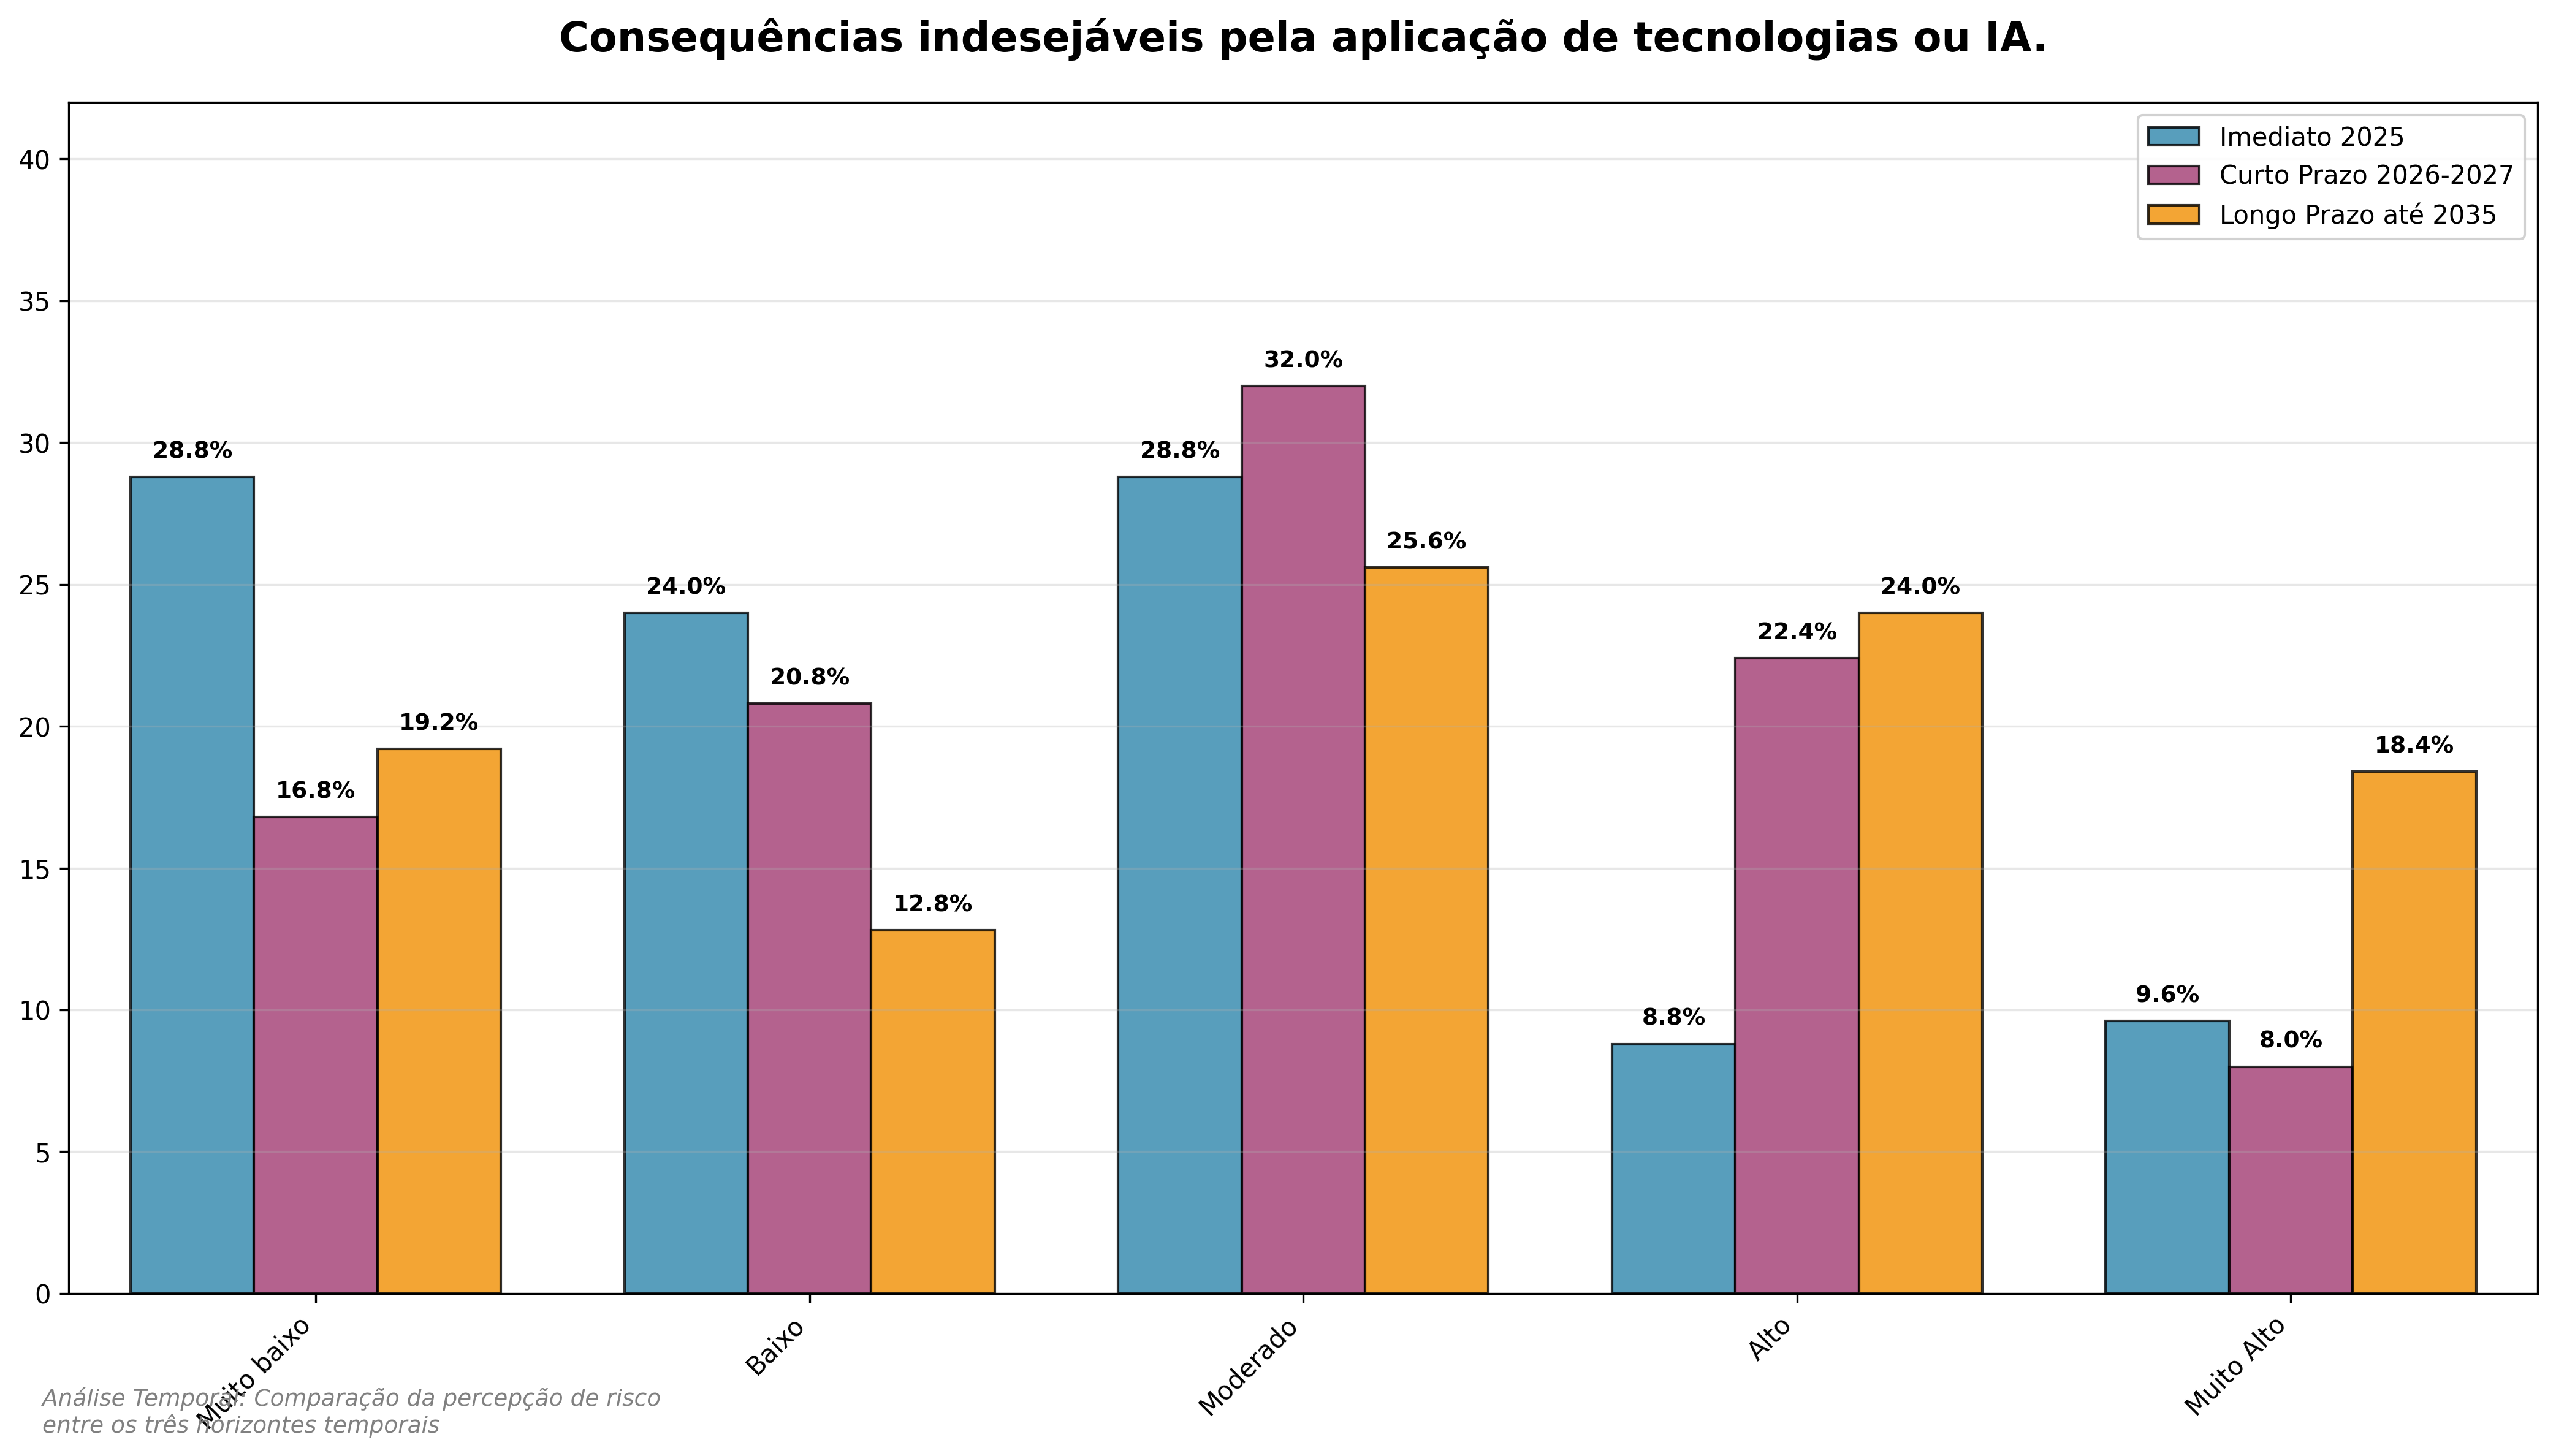
\includegraphics[keepaspectratio]{assets/tecnologicos/grafico_agrupado_5_1_temporal.png}}

\begin{tcolorbox}[enhanced jigsaw, titlerule=0mm, colback=white, title=\textcolor{quarto-callout-tip-color}{\faLightbulb}\hspace{0.5em}{Destaques}, opacityback=0, colbacktitle=quarto-callout-tip-color!10!white, leftrule=.75mm, left=2mm, colframe=quarto-callout-tip-color-frame, bottomrule=.15mm, bottomtitle=1mm, breakable, toprule=.15mm, toptitle=1mm, opacitybacktitle=0.6, arc=.35mm, coltitle=black, rightrule=.15mm]

\textbf{Imediato (2025)}: Mediana 2.0, 18\% em risco alto

\textbf{Curto Prazo (2026-2027)}: Mediana 3.0, 30\% em risco alto

\textbf{Longo Prazo (até 2035)}: Mediana 3.0, 42\% em risco alto

\begin{itemize}
\tightlist
\item
  \textbf{Tendência}: Percepção de risco relativamente estável ao longo
  do tempo. \textbf{Análise - Consequências indesejáveis pela aplicação
  de tecnologias ou IA} \textbf{Imediato (2025)}: Devido a consequências
  iniciais pela aplicação de tecnologias ou IA, poderá acontecer a
  ocorrência pontual de falhas ou vieses limitados, o que poderá levar a
  decisões não ideais ou pequenos incidentes operacionais, impactando de
  forma controlada a eficiência e segurança das operações portuárias
  brasileiras.
\end{itemize}

\textbf{Curto prazo (2026-2027)}: Devido a consequências indesejáveis
pela aplicação de tecnologias ou IA no setor portuário brasileiro,
poderá acontecer a ocorrência de falhas operacionais, vieses
algorítmicos ou usos indevidos, o que poderá levar a decisões não
ideais, discriminações pontuais ou vulnerabilidades de segurança,
impactando de forma moderada a eficiência, equidade e integridade das
operações portuárias no curto prazo (2026 a 2027).

\textbf{Longo prazo (até 2035)}: Devido a consequências indesejáveis
pela aplicação de tecnologias ou IA no setor portuário brasileiro,
poderá acontecer a ocorrência de falhas sistemáticas, vieses
operacionais ou usos indevidos, o que poderá levar a decisões não
ideais, discriminação setorial ou falhas de segurança cibernética,
impactando de forma moderada a eficiência, equidade e segurança das
operações portuárias ao longo do horizonte até 2035, demandando
monitoramento contínuo e aprimoramento das práticas de governança
tecnológica.

\end{tcolorbox}

\subsection{Consequências adversas de tecnologias avançadas (física,
biotecnologia,
geoengenharia)}\label{consequuxeancias-adversas-de-tecnologias-avanuxe7adas-fuxedsica-biotecnologia-geoengenharia}

O gr?fico a seguir apresenta a evolu??o temporal do risco Consequências
adversas de tecnologias avançadas (física, biotecnologia,
geoengenharia).
\pandocbounded{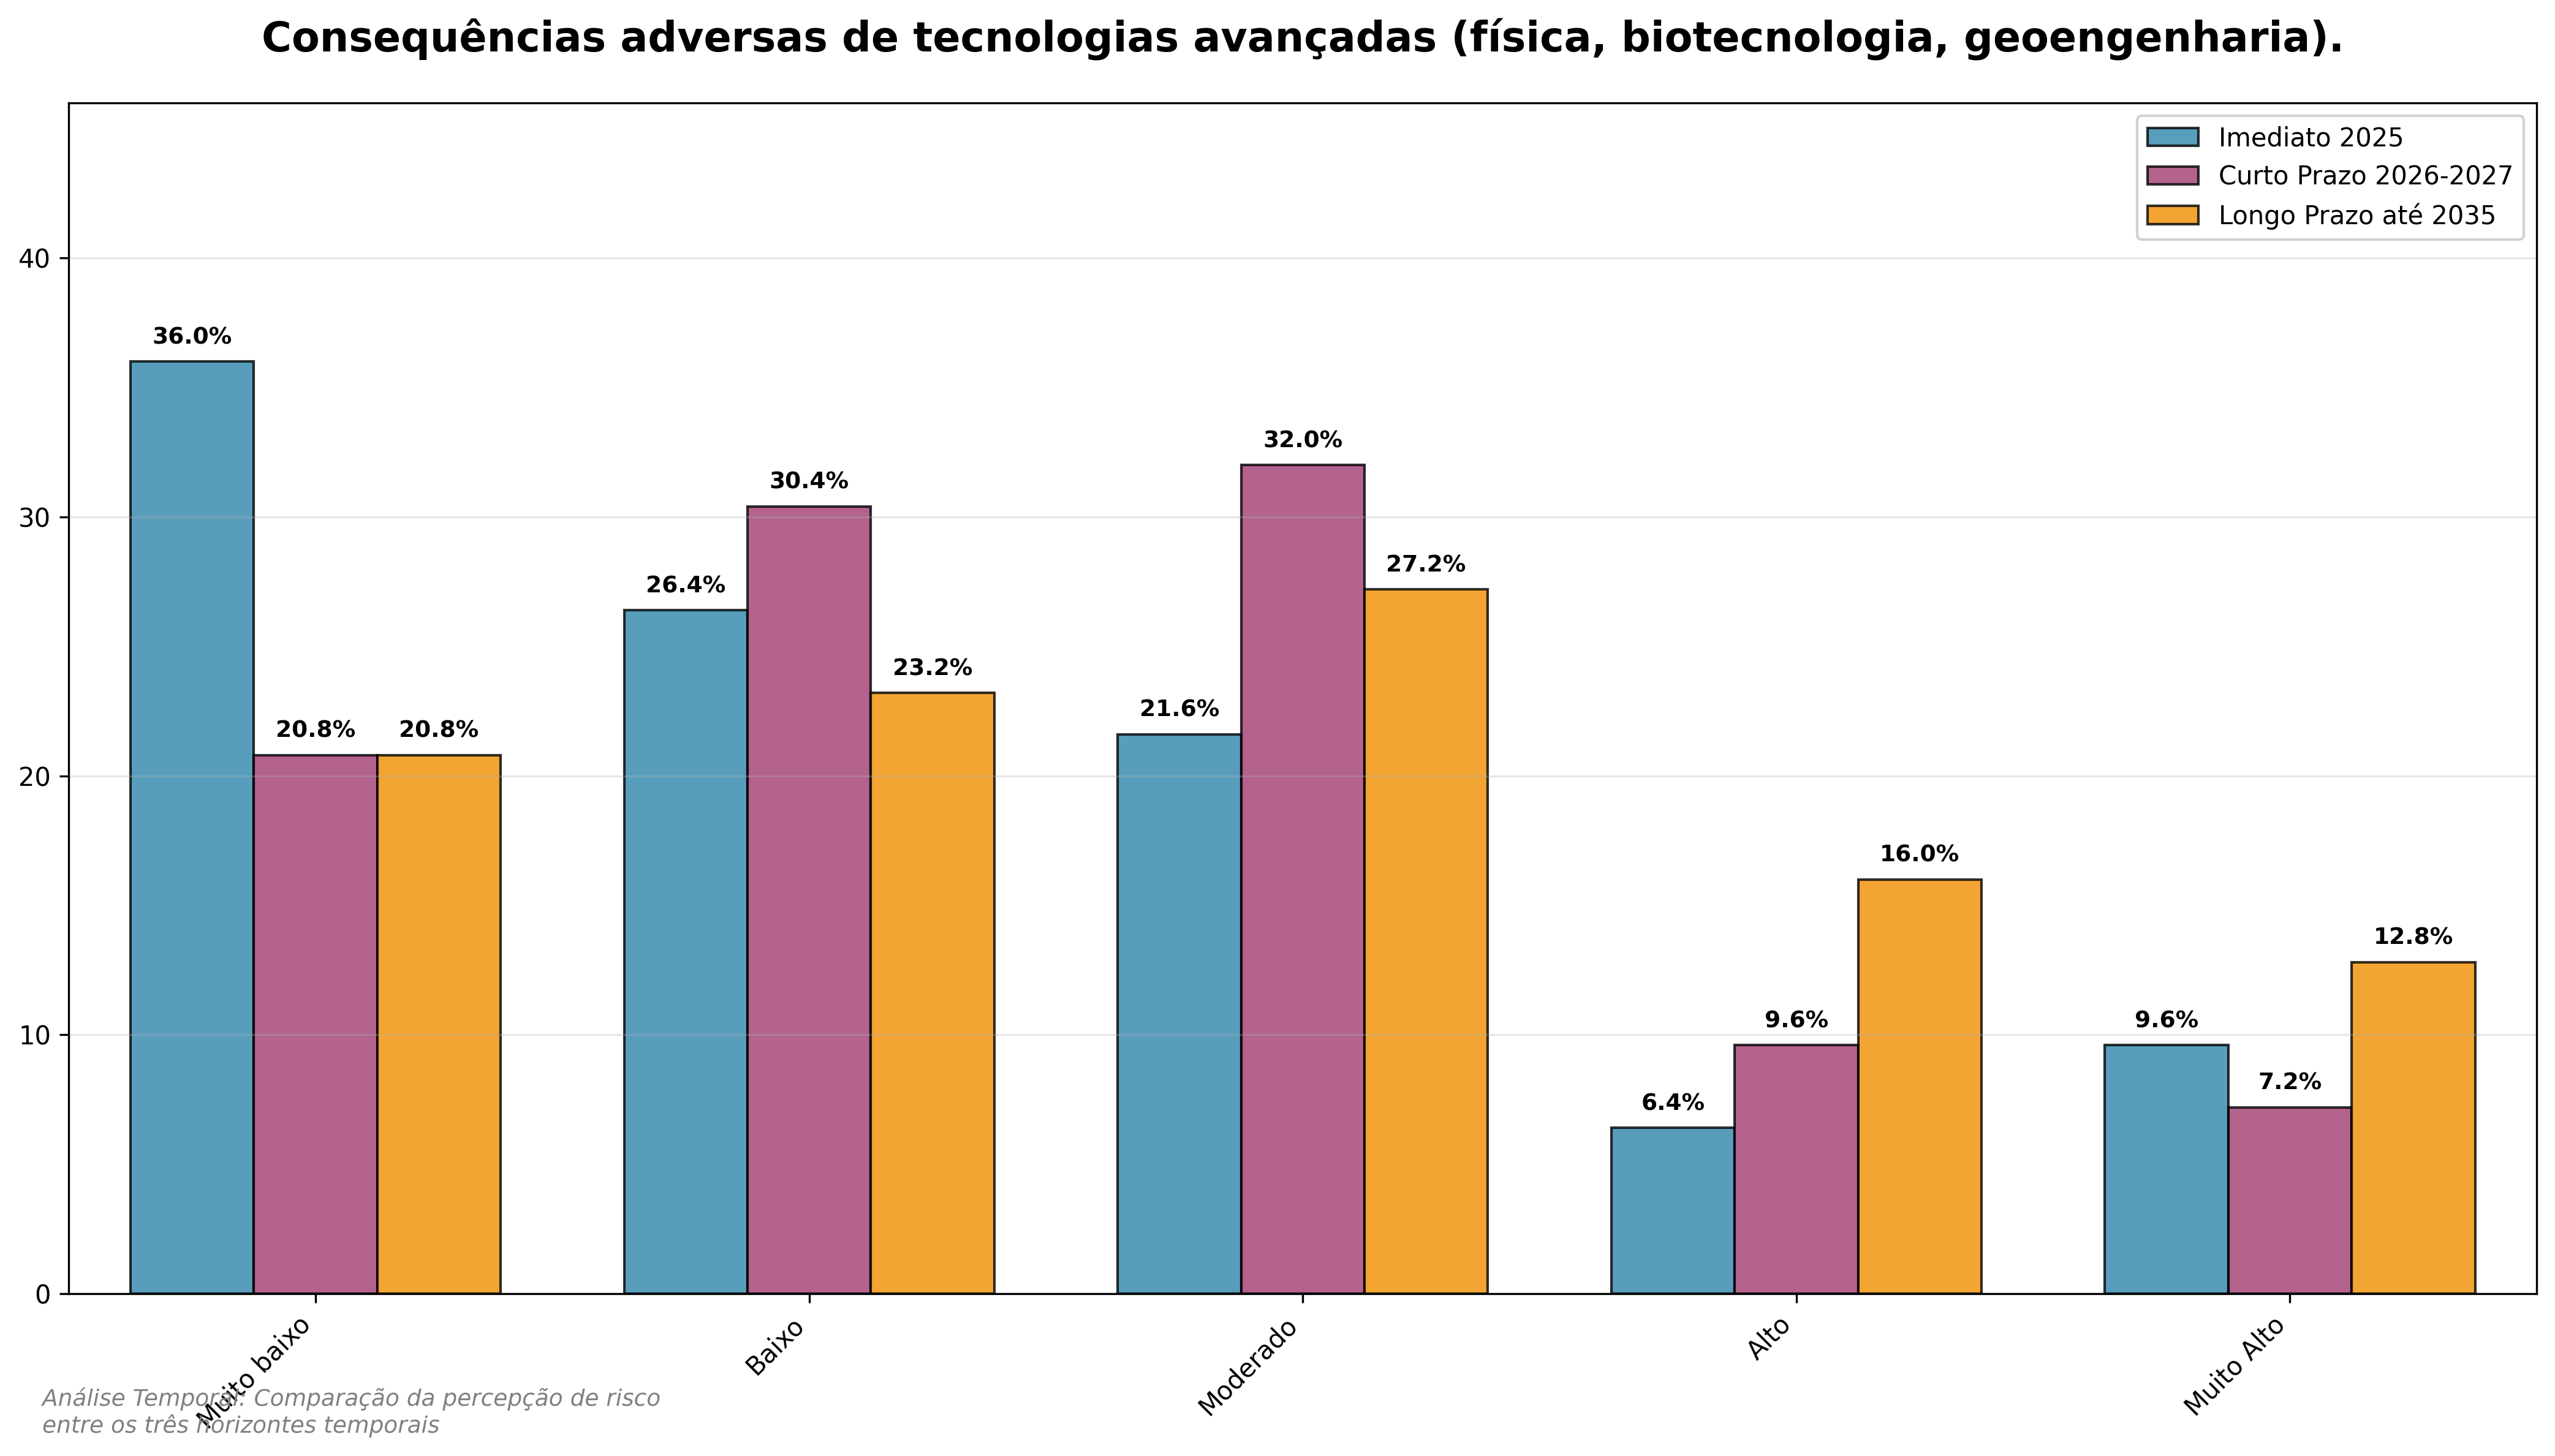
\includegraphics[keepaspectratio]{assets/tecnologicos/grafico_agrupado_5_2_temporal.png}}

\begin{tcolorbox}[enhanced jigsaw, titlerule=0mm, colback=white, title=\textcolor{quarto-callout-tip-color}{\faLightbulb}\hspace{0.5em}{Destaques}, opacityback=0, colbacktitle=quarto-callout-tip-color!10!white, leftrule=.75mm, left=2mm, colframe=quarto-callout-tip-color-frame, bottomrule=.15mm, bottomtitle=1mm, breakable, toprule=.15mm, toptitle=1mm, opacitybacktitle=0.6, arc=.35mm, coltitle=black, rightrule=.15mm]

\textbf{Imediato (2025)}: Mediana 2.0, 16\% em risco alto

\textbf{Curto Prazo (2026-2027)}: Mediana 2.0, 17\% em risco alto

\textbf{Longo Prazo (até 2035)}: Mediana 3.0, 29\% em risco alto

\textbf{Análise - Consequências adversas de tecnologias avançadas
(física, biotecnologia, geoengenharia)} \textbf{Imediato (2025)}: Devido
a consequências iniciais relacionadas ao uso de tecnologias avançadas
(física, biotecnologia, geoengenharia), poderá ocorrer o emprego
inadequado ou pouco controlado dessas tecnologias, o que poderá levar a
impactos ambientais, sociais e econômicos limitados, com efeitos
restritos à sustentabilidade e à segurança das operações portuárias e de
seu entorno no setor brasileiro.

\textbf{Curto prazo (2026-2027)}: Devido a consequências iniciais
relacionadas a tecnologias avançadas (física, biotecnologia,
geoengenharia), poderá ocorrer o uso inadequado ou pouco monitorado
dessas inovações, o que poderá levar a impactos ambientais, sociais e
operacionais limitados, impactando de forma controlável a
sustentabilidade e a segurança das operações portuárias brasileiras e
seu entorno.

\textbf{Longo prazo (até 2035)}: Devido a consequências adversas de
tecnologias avançadas (física, biotecnologia, geoengenharia), poderá
acontecer o uso inadequado ou insuficientemente regulado dessas
tecnologias no ambiente portuário brasileiro, o que poderá levar a
impactos ambientais e sociais moderados, além de desafios operacionais e
econômicos, impactando na sustentabilidade e na segurança das operações
portuárias e do seu entorno ao longo do período até 2035.

\end{tcolorbox}

\subsection{Consequências indesejáveis pela aplicação de tecnologias ou
IA (censura e
vigilância)}\label{consequuxeancias-indesejuxe1veis-pela-aplicauxe7uxe3o-de-tecnologias-ou-ia-censura-e-vigiluxe2ncia}

O gr?fico a seguir apresenta a evolu??o temporal do risco Consequências
indesejáveis pela aplicação de tecnologias ou IA (censura e vigilância).
\pandocbounded{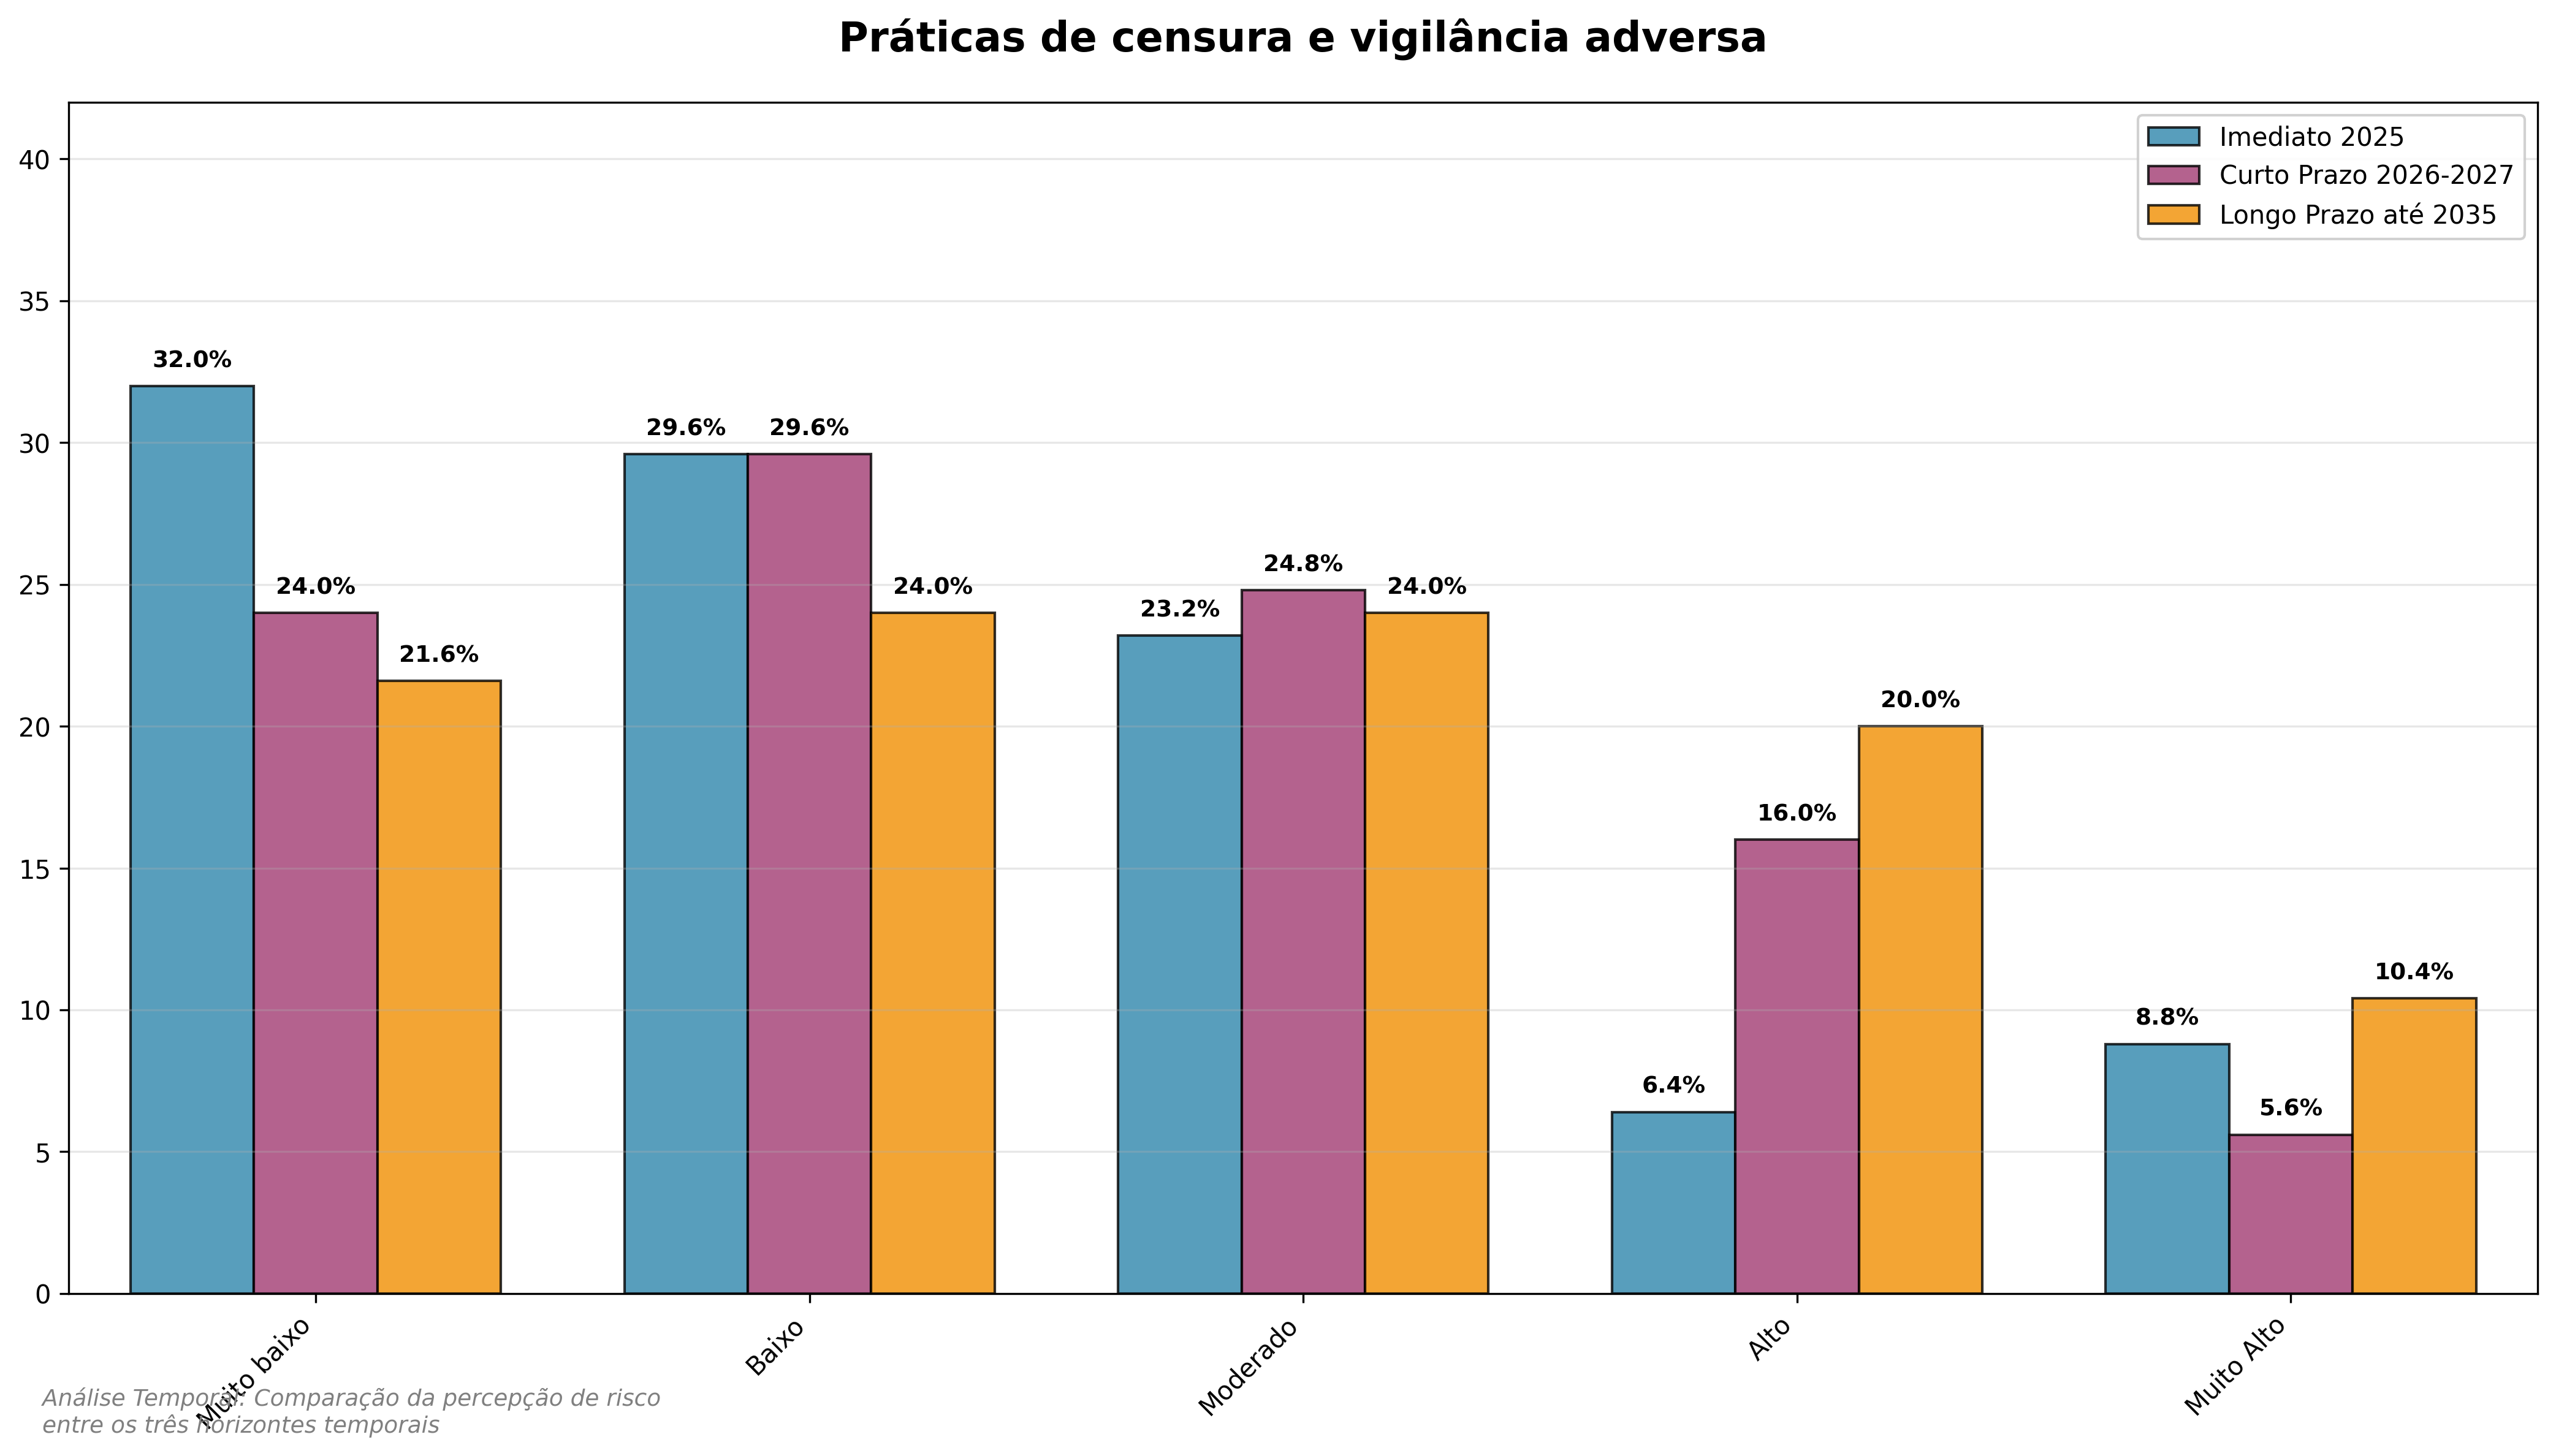
\includegraphics[keepaspectratio]{assets/tecnologicos/grafico_agrupado_5_3_temporal.png}}

\begin{tcolorbox}[enhanced jigsaw, titlerule=0mm, colback=white, title=\textcolor{quarto-callout-tip-color}{\faLightbulb}\hspace{0.5em}{Destaques}, opacityback=0, colbacktitle=quarto-callout-tip-color!10!white, leftrule=.75mm, left=2mm, colframe=quarto-callout-tip-color-frame, bottomrule=.15mm, bottomtitle=1mm, breakable, toprule=.15mm, toptitle=1mm, opacitybacktitle=0.6, arc=.35mm, coltitle=black, rightrule=.15mm]

\textbf{Imediato (2025)}: Mediana 2.0, 15\% em risco alto

\textbf{Curto Prazo (2026-2027)}: Mediana 2.0, 22\% em risco alto

\textbf{Longo Prazo (até 2035)}: Mediana 3.0, 30\% em risco alto

\textbf{Análise - Práticas de censura e vigilância adversa}
\textbf{Imediato (2025)}: Devido a práticas iniciais de censura e
vigilância no setor portuário brasileiro, poderá acontecer restrições
pontuais na divulgação de informações sensíveis e monitoramento
moderado, o que poderá levar a limitações na privacidade de
trabalhadores e comunidades, impactando de forma restrita os direitos
individuais e a transparência do setor.

\textbf{Curto prazo (2026-2027)}: Devido a práticas iniciais de censura
e vigilância no setor portuário brasileiro, poderá acontecer restrições
pontuais na divulgação de informações sensíveis e monitoramento
moderado, o que poderá levar a impactos limitados na privacidade de
trabalhadores e comunidades, afetando de forma controlada os direitos
individuais e a transparência do setor no curto prazo (2026 a 2027).

\textbf{Longo prazo (até 2035)}: Devido a práticas persistentes de
censura e vigilância adversa no setor portuário brasileiro, poderá
acontecer restrições moderadas na divulgação de informações sensíveis e
monitoramento contínuo, o que poderá levar a um comprometimento parcial
da privacidade de trabalhadores e comunidades locais, impactando nos
direitos individuais e na transparência operacional ao longo do período
até 2035.

\end{tcolorbox}

\subsection{Falta de segurança computacional e de
comunicação}\label{falta-de-seguranuxe7a-computacional-e-de-comunicauxe7uxe3o}

O gr?fico a seguir apresenta a evolu??o temporal do risco Falta de
segurança computacional e de comunicação.
\pandocbounded{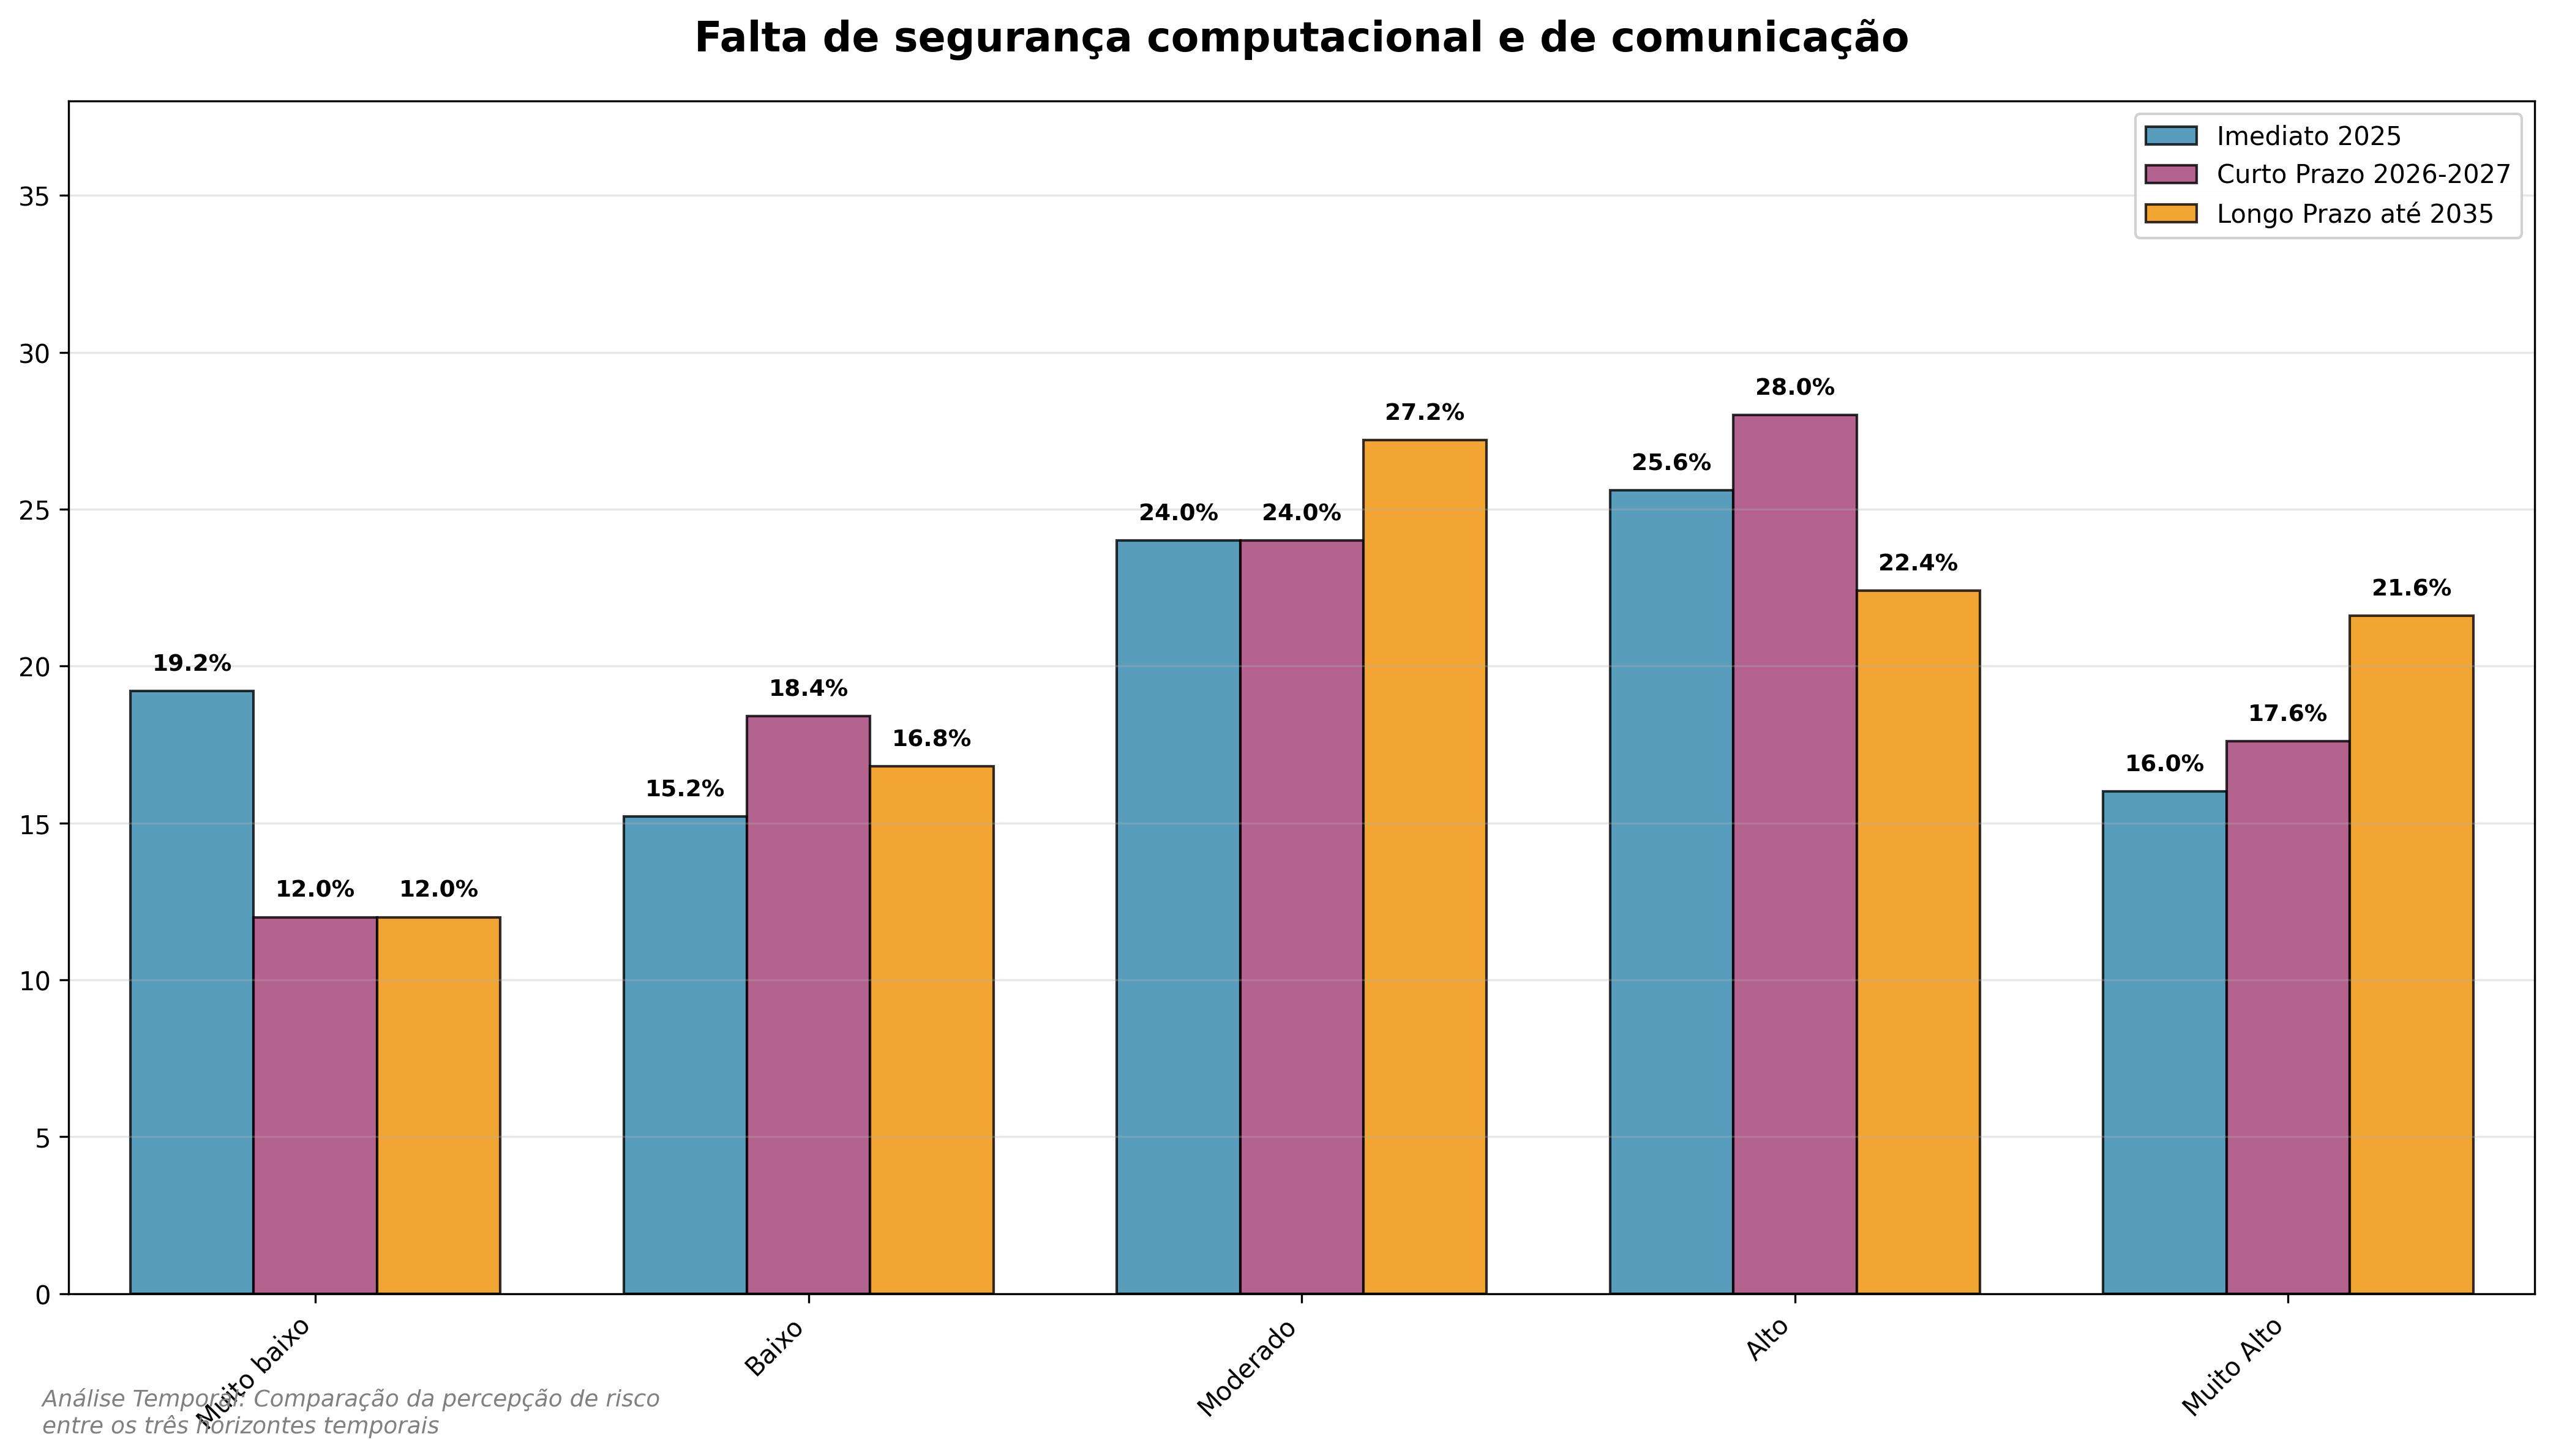
\includegraphics[keepaspectratio]{assets/tecnologicos/grafico_agrupado_5_4_temporal.png}}

\begin{tcolorbox}[enhanced jigsaw, titlerule=0mm, colback=white, title=\textcolor{quarto-callout-tip-color}{\faLightbulb}\hspace{0.5em}{Destaques}, opacityback=0, colbacktitle=quarto-callout-tip-color!10!white, leftrule=.75mm, left=2mm, colframe=quarto-callout-tip-color-frame, bottomrule=.15mm, bottomtitle=1mm, breakable, toprule=.15mm, toptitle=1mm, opacitybacktitle=0.6, arc=.35mm, coltitle=black, rightrule=.15mm]

\textbf{Imediato (2025)}: Mediana 3.0, 42\% em risco alto

\textbf{Curto Prazo (2026-2027)}: Mediana 3.0, 46\% em risco alto

\textbf{Longo Prazo (até 2035)}: Mediana 3.0, 44\% em risco alto

\textbf{Análise - Falta de segurança computacional e de comunicação}
\textbf{Imediato (2025)}: Devido a vulnerabilidades ainda presentes na
segurança computacional e de comunicação, poderão ocorrer incidentes
cibernéticos como tentativas de invasão e interrupções temporárias nos
sistemas, o que poderá levar à alteração parcial de dados operacionais
ou à indisponibilidade momentânea de serviços essenciais, impactando a
eficiência e a continuidade das operações nos portos brasileiros.

\textbf{Curto prazo (2026-2027)}: Devido à persistente vulnerabilidade
em segurança computacional e de comunicação nos portos brasileiros,
poderá ocorrer incidentes cibernéticos moderados, como tentativas de
invasão e comprometimento parcial de dados, o que poderá levar à
interrupção temporária de sistemas operacionais ou à degradação da
integridade das informações, impactando a eficiência e a continuidade
das operações portuárias no curto prazo.

\textbf{Longo prazo (até 2035)}: Devido a vulnerabilidades persistentes
na segurança computacional e de comunicação, poderá acontecer incidentes
cibernéticos como invasões e interrupções de sistemas, o que poderá
levar à manipulação de dados operacionais ou indisponibilidade
temporária de plataformas digitais, impactando a eficiência e a
continuidade das operações nos terminais portuários brasileiros.

\end{tcolorbox}

\subsection{Concentração dos direitos sobre
tecnologias}\label{concentrauxe7uxe3o-dos-direitos-sobre-tecnologias}

O gr?fico a seguir apresenta a evolu??o temporal do risco Concentração
dos direitos sobre tecnologias.
\pandocbounded{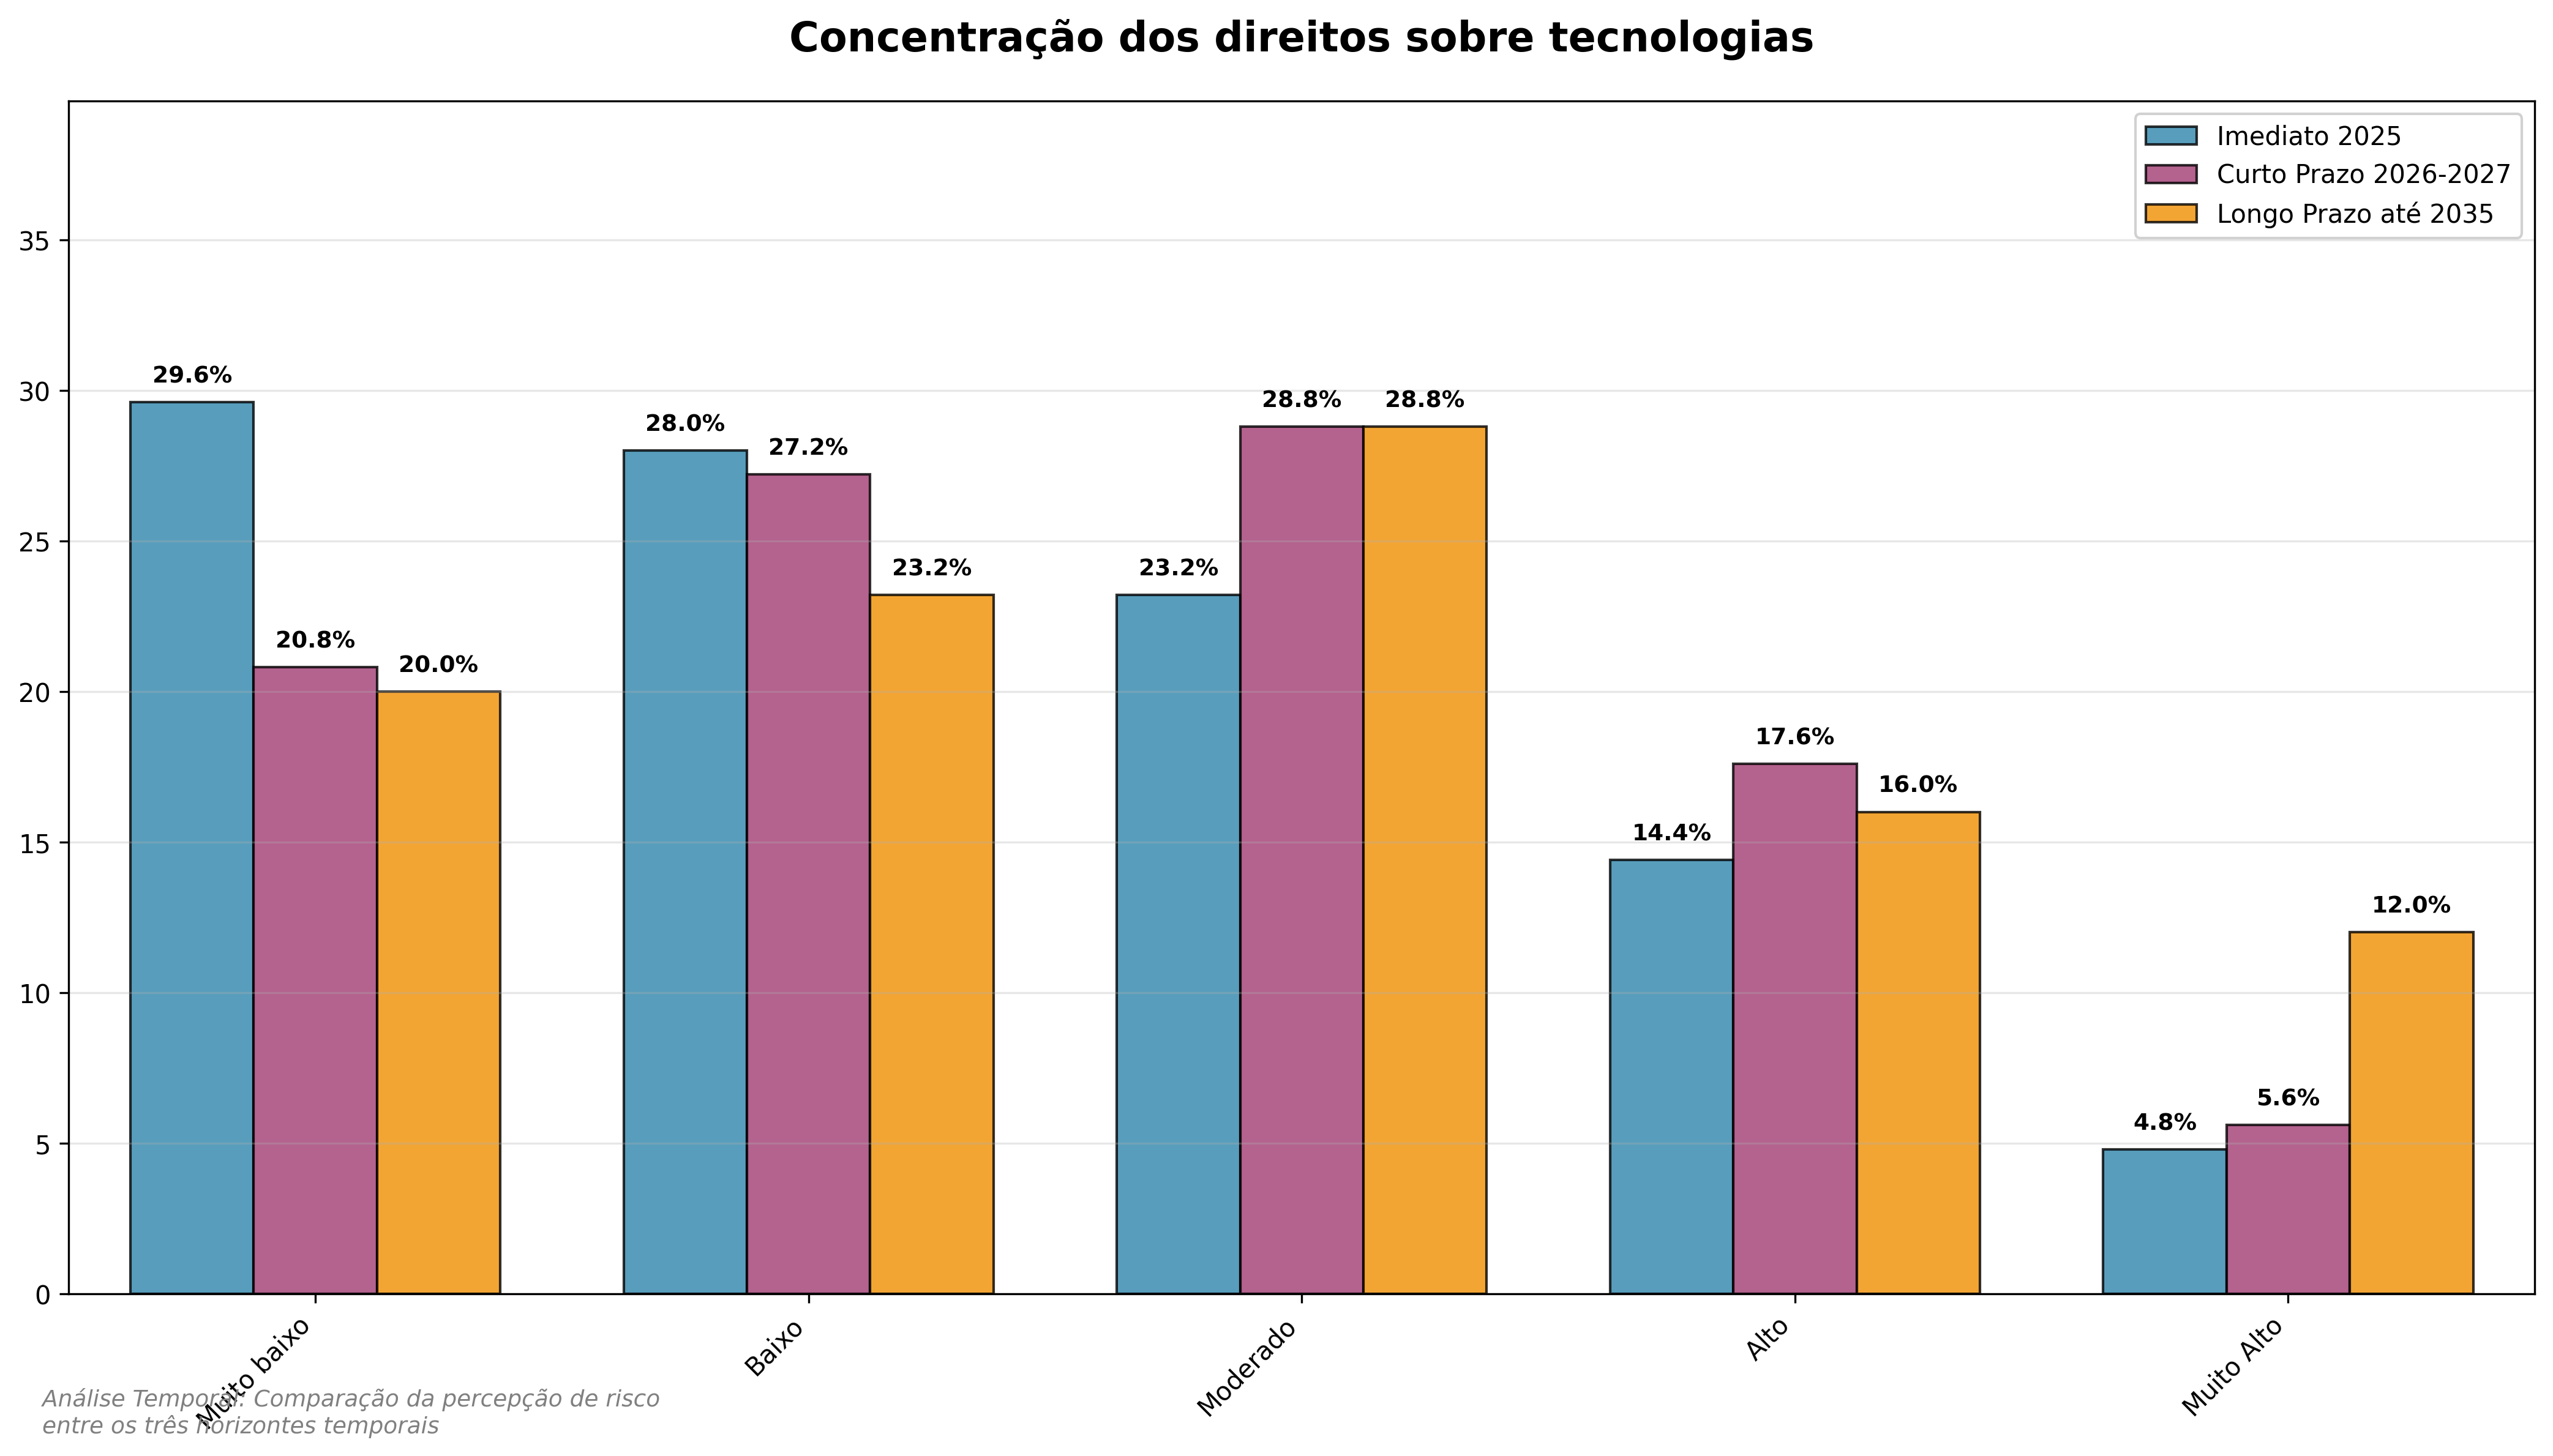
\includegraphics[keepaspectratio]{assets/tecnologicos/grafico_agrupado_5_5_temporal.png}}

\begin{tcolorbox}[enhanced jigsaw, titlerule=0mm, colback=white, title=\textcolor{quarto-callout-tip-color}{\faLightbulb}\hspace{0.5em}{Destaques}, opacityback=0, colbacktitle=quarto-callout-tip-color!10!white, leftrule=.75mm, left=2mm, colframe=quarto-callout-tip-color-frame, bottomrule=.15mm, bottomtitle=1mm, breakable, toprule=.15mm, toptitle=1mm, opacitybacktitle=0.6, arc=.35mm, coltitle=black, rightrule=.15mm]

\textbf{Imediato (2025)}: Mediana 2.0, 19\% em risco alto

\textbf{Curto Prazo (2026-2027)}: Mediana 3.0, 23\% em risco alto

\textbf{Longo Prazo (até 2035)}: Mediana 3.0, 28\% em risco alto

\textbf{Análise - Concentração dos direitos sobre tecnologias}
\textbf{Imediato (2025)}: Devido à crescente concentração dos direitos
sobre tecnologias, poderá acontecer uma leve dependência tecnológica e
restrições iniciais ao acesso a inovações, o que poderá levar a desafios
pontuais na modernização e a uma autonomia estratégica ainda preservada,
impactando de forma limitada a competitividade e o desenvolvimento dos
portos brasileiros no curto prazo.

\textbf{Curto prazo (2026-2027)}: Devido à concentração dos direitos
sobre tecnologias, poderá ocorrer uma dependência moderada de
fornecedores externos e restrições no acesso a inovações tecnológicas, o
que poderá levar a desafios na atualização dos sistemas portuários e
limitações na autonomia operacional, impactando a eficiência e a
competitividade dos portos brasileiros no curto prazo.

\textbf{Longo prazo (até 2035)}: Devido à concentração dos direitos
sobre tecnologias, poderá ocorrer uma dependência moderada de
fornecedores externos, limitando o acesso a inovações tecnológicas e
dificultando a incorporação de avanços nos sistemas portuários
brasileiros, o que poderá levar a desafios na modernização e na
manutenção da autonomia estratégica, impactando de forma moderada a
eficiência operacional e a competitividade dos portos no longo prazo.

\end{tcolorbox}

\subsection{Vulnerabilidades dos sistemas de comunicação e dispositivos
IoT}\label{vulnerabilidades-dos-sistemas-de-comunicauxe7uxe3o-e-dispositivos-iot}

O gr?fico a seguir apresenta a evolu??o temporal do risco
Vulnerabilidades dos sistemas de comunicação e dispositivos IoT.
\pandocbounded{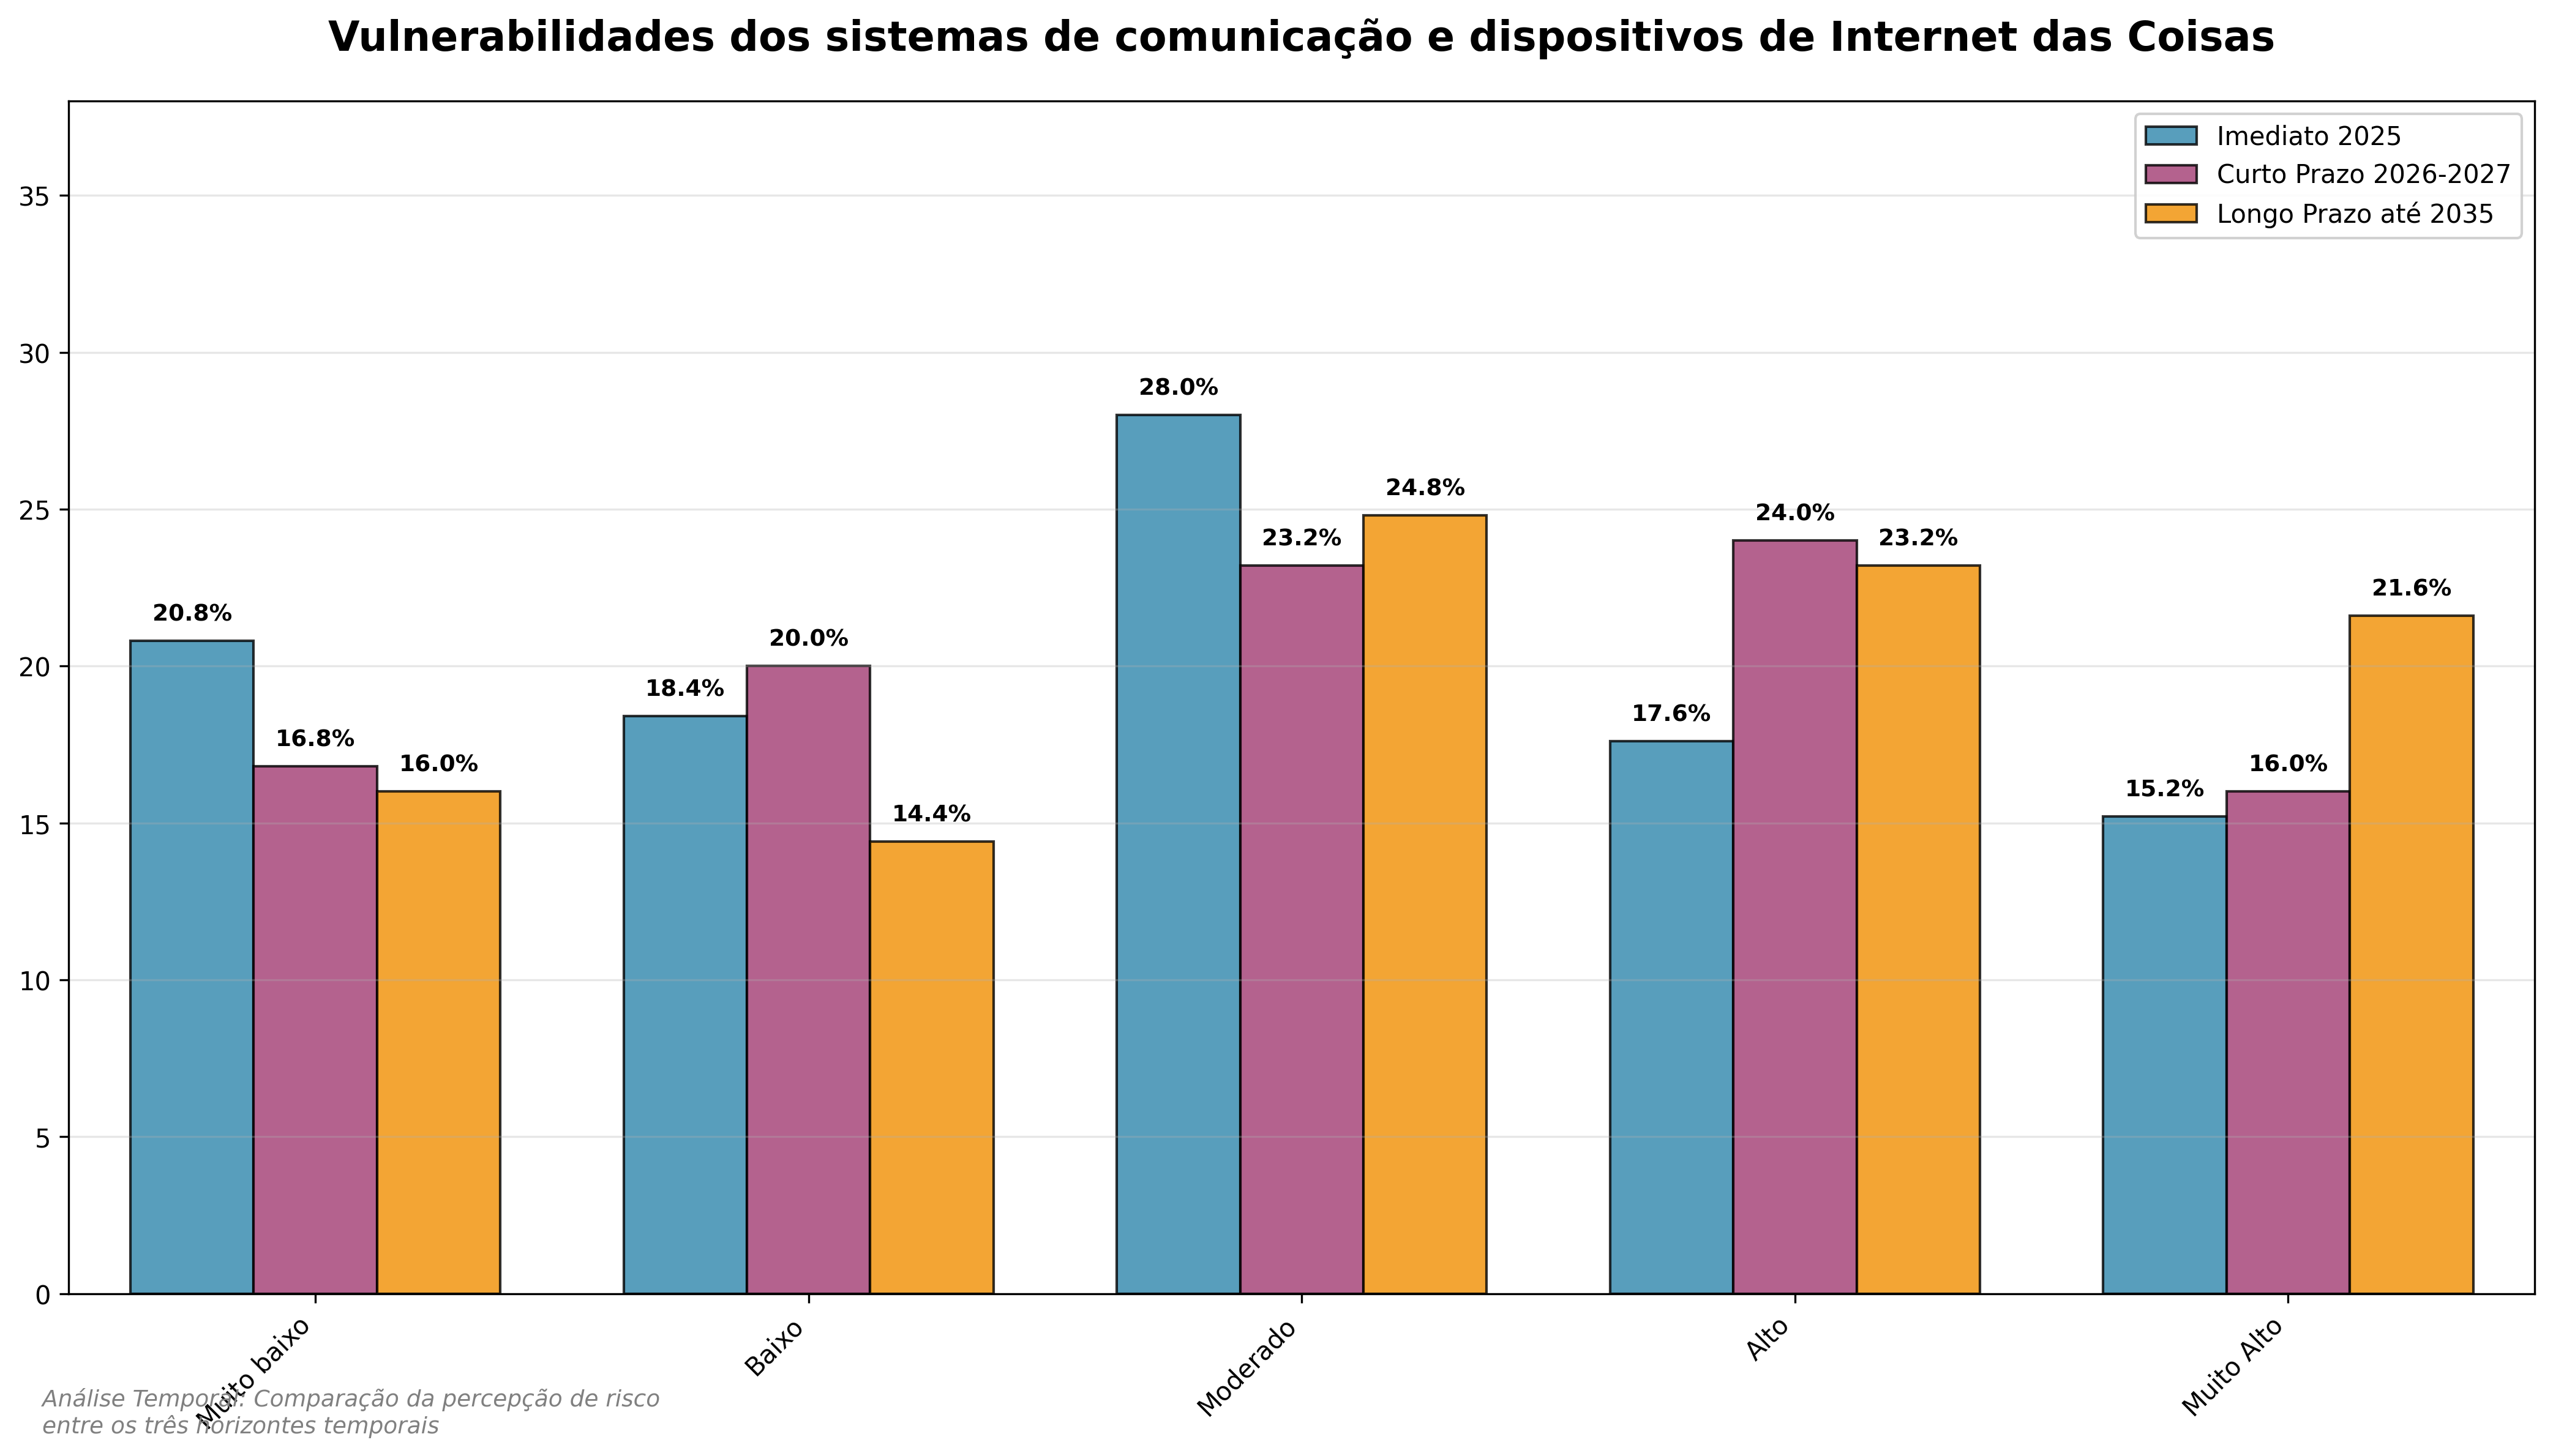
\includegraphics[keepaspectratio]{assets/tecnologicos/grafico_agrupado_5_6_temporal.png}}

\begin{tcolorbox}[enhanced jigsaw, titlerule=0mm, colback=white, title=\textcolor{quarto-callout-tip-color}{\faLightbulb}\hspace{0.5em}{Destaques}, opacityback=0, colbacktitle=quarto-callout-tip-color!10!white, leftrule=.75mm, left=2mm, colframe=quarto-callout-tip-color-frame, bottomrule=.15mm, bottomtitle=1mm, breakable, toprule=.15mm, toptitle=1mm, opacitybacktitle=0.6, arc=.35mm, coltitle=black, rightrule=.15mm]

\textbf{Imediato (2025)}: Mediana 3.0, 33\% em risco alto

\textbf{Curto Prazo (2026-2027)}: Mediana 3.0, 40\% em risco alto

\textbf{Longo Prazo (até 2035)}: Mediana 3.0, 45\% em risco alto

\begin{itemize}
\tightlist
\item
  \textbf{Tendência}: Percepção de risco relativamente estável ao longo
  do tempo. \textbf{Análise - Vulnerabilidades dos sistemas de
  comunicação e dispositivos IoT} \textbf{Imediato (2025)}: Devido a
  vulnerabilidades conhecidas nos sistemas de comunicação e dispositivos
  IoT utilizados em terminais e operações portuárias brasileiras, poderá
  acontecer incidentes de cibersegurança com interrupções pontuais nos
  serviços, o que poderá levar a atrasos operacionais e aumento dos
  riscos à integridade das operações, impactando a eficiência e a
  segurança no curto prazo.
\end{itemize}

\textbf{Curto prazo (2026-2027)}: Devido a vulnerabilidades existentes
nos sistemas de comunicação e dispositivos de Internet das Coisas (IoT)
utilizados nas operações portuárias brasileiras, poderá acontecer falhas
moderadas em cibersegurança, o que poderá levar a ataques cibernéticos
localizados e interrupções parciais de serviços, impactando na segurança
operacional e na continuidade das atividades portuárias no curto prazo
(2026 a 2027).

\textbf{Longo prazo (até 2035)}: Devido a vulnerabilidades persistentes
nos sistemas de comunicação e dispositivos de Internet das Coisas (IoT)
utilizados no setor portuário brasileiro, poderá acontecer falhas de
cibersegurança com frequência moderada, o que poderá levar a incidentes
cibernéticos que causem interrupções temporárias nos serviços e afetem a
eficiência operacional, requerendo monitoramento contínuo e estratégias
de mitigação para assegurar a resiliência das operações até 2035.

\end{tcolorbox}

\subsection{Atraso no processo de digitalização dos
portos}\label{atraso-no-processo-de-digitalizauxe7uxe3o-dos-portos}

O gr?fico a seguir apresenta a evolu??o temporal do risco Atraso no
processo de digitalização dos portos.
\pandocbounded{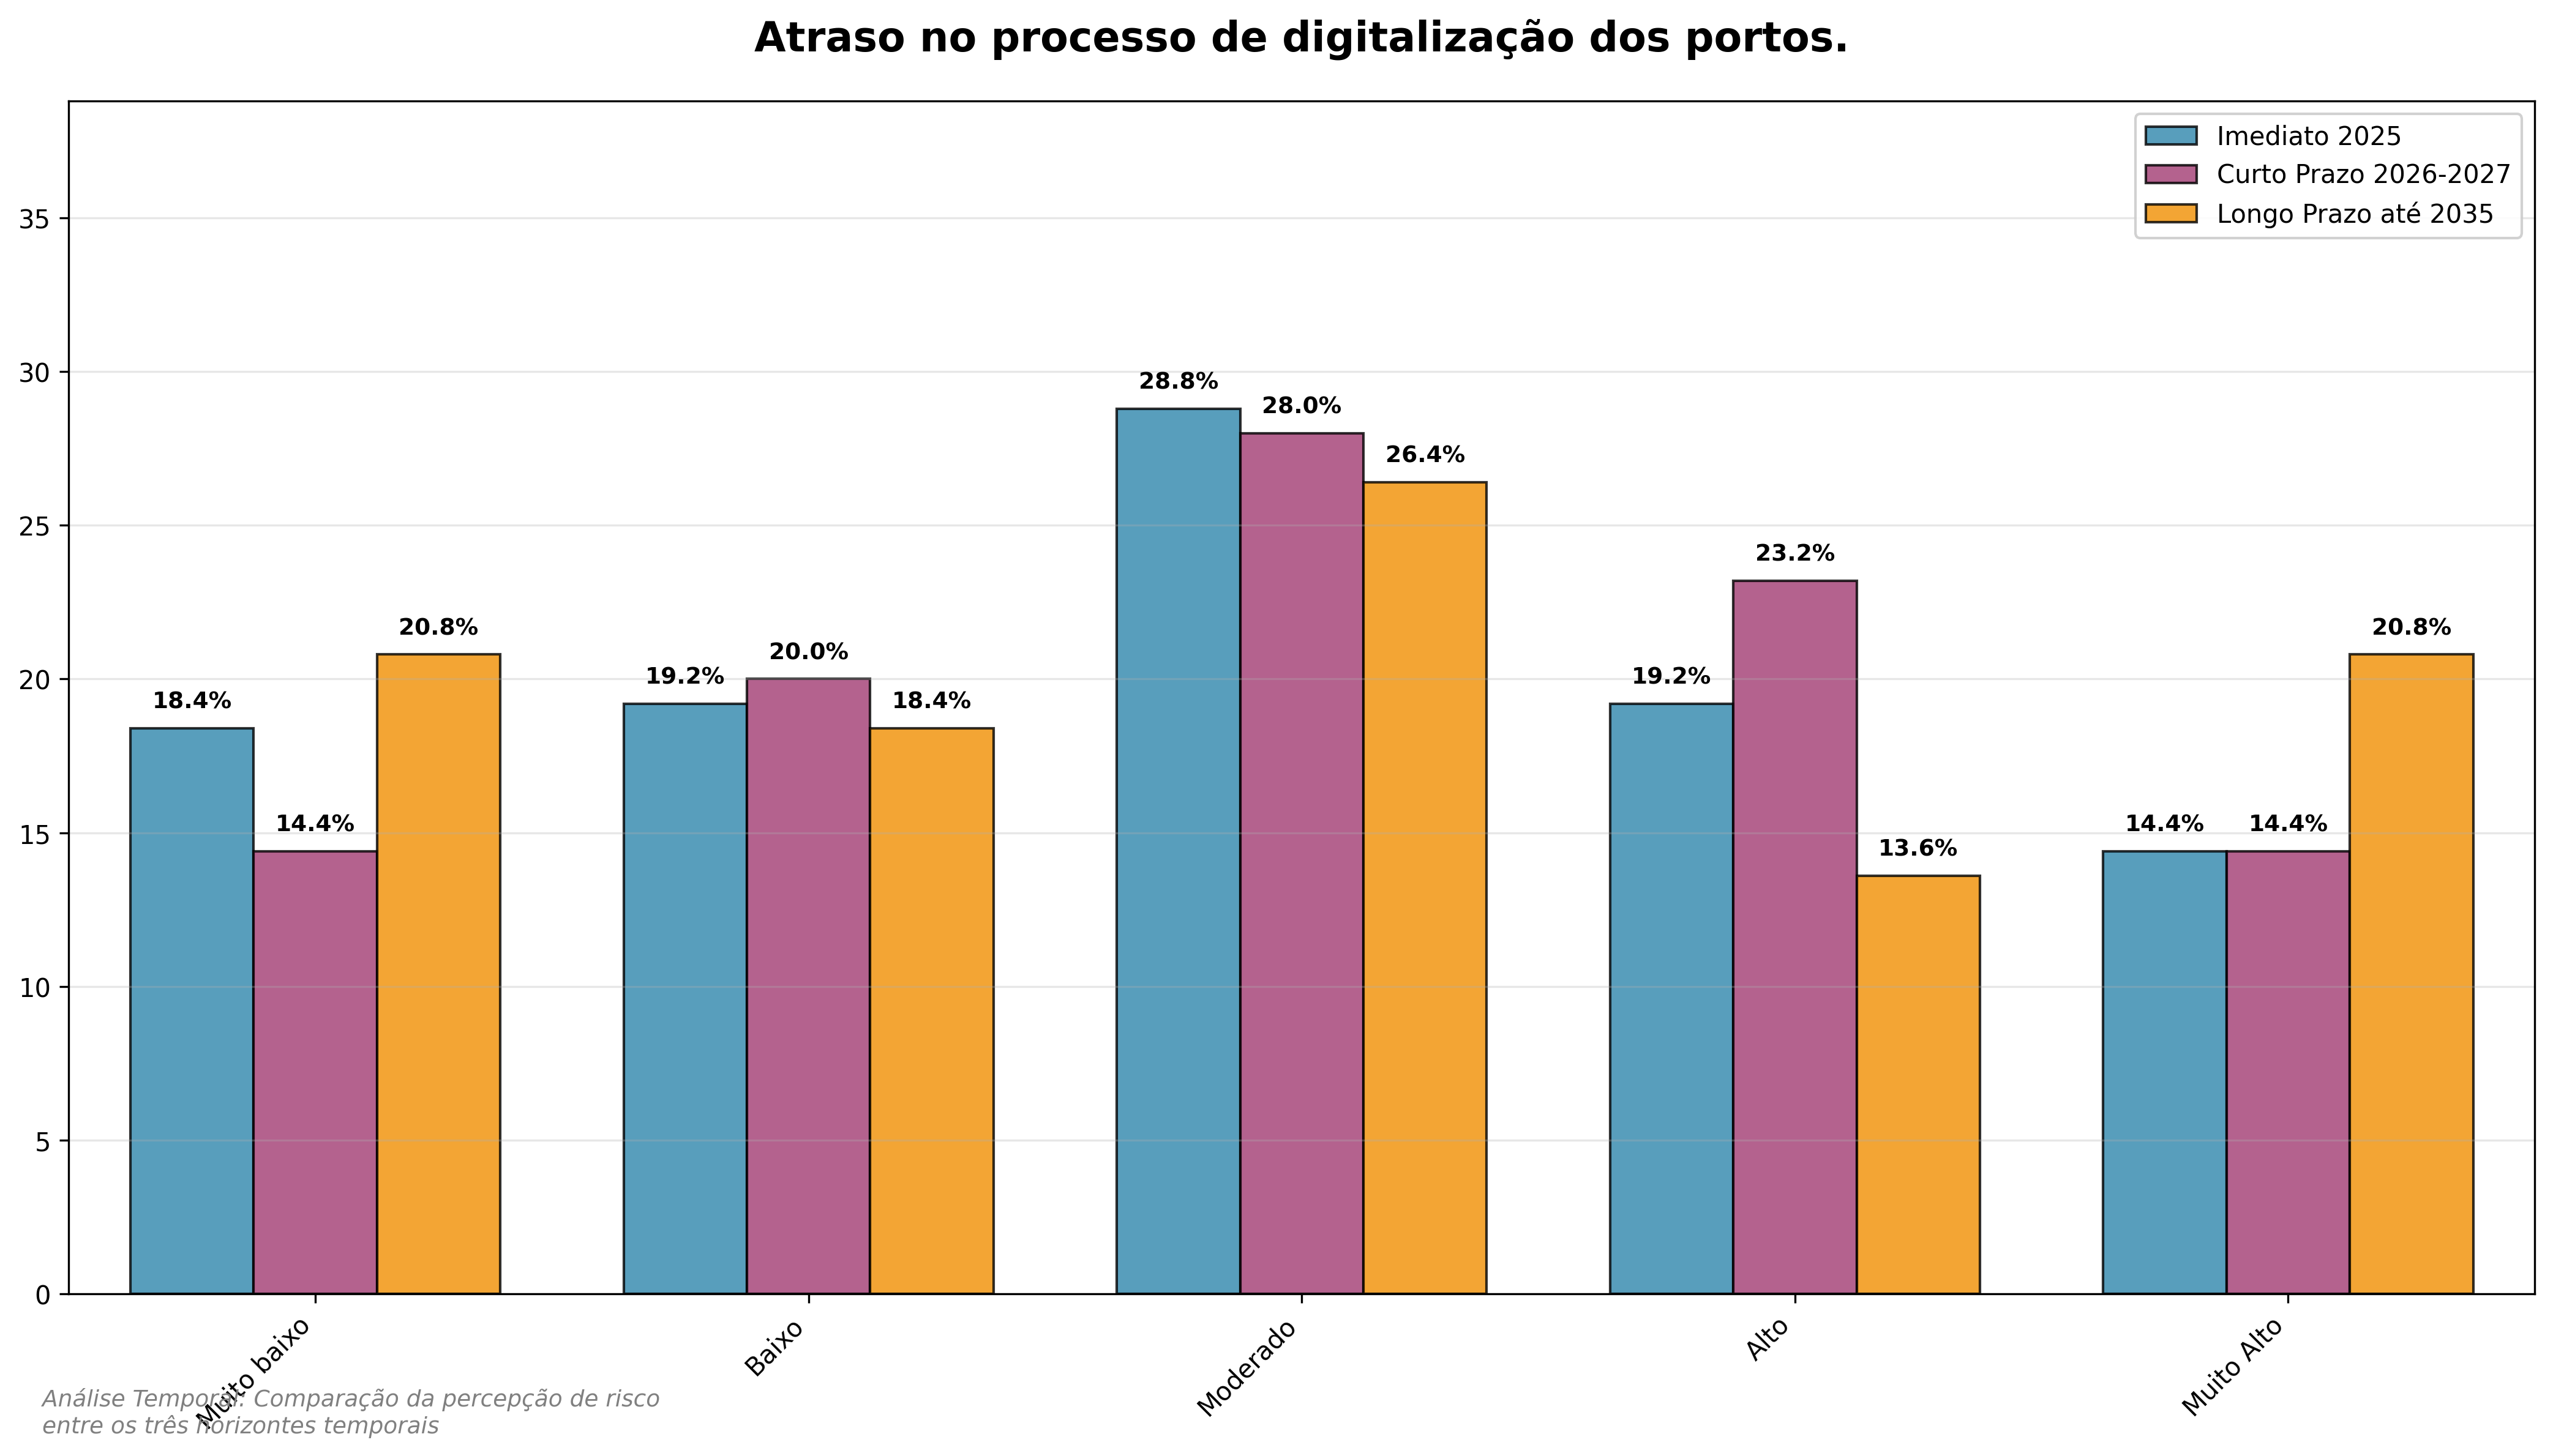
\includegraphics[keepaspectratio]{assets/tecnologicos/grafico_agrupado_5_7_temporal.png}}

\begin{tcolorbox}[enhanced jigsaw, titlerule=0mm, colback=white, title=\textcolor{quarto-callout-tip-color}{\faLightbulb}\hspace{0.5em}{Destaques}, opacityback=0, colbacktitle=quarto-callout-tip-color!10!white, leftrule=.75mm, left=2mm, colframe=quarto-callout-tip-color-frame, bottomrule=.15mm, bottomtitle=1mm, breakable, toprule=.15mm, toptitle=1mm, opacitybacktitle=0.6, arc=.35mm, coltitle=black, rightrule=.15mm]

\textbf{Imediato (2025)}: Mediana 3.0, 34\% em risco alto

\textbf{Curto Prazo (2026-2027)}: Mediana 3.0, 38\% em risco alto

\textbf{Longo Prazo (até 2035)}: Mediana 3.0, 34\% em risco alto

\begin{itemize}
\tightlist
\item
  \textbf{Tendência}: Percepção de risco relativamente estável ao longo
  do tempo. \textbf{Análise - Atraso no processo de digitalização dos
  portos} \textbf{Imediato (2025)}: Devido ao ritmo moderado no avanço
  da digitalização dos portos brasileiros, poderá ocorrer redução
  parcial na eficiência operacional e na capacidade de integração com
  cadeias logísticas globais, o que poderá levar a aumentos controlados
  nos custos e a limitações na competitividade do setor, impactando de
  forma moderada o desenvolvimento econômico e a modernização portuária
  no curto prazo.
\end{itemize}

\textbf{Curto prazo (2026-2027)}: Devido a atrasos moderados no processo
de digitalização dos portos brasileiros, poderá acontecer uma redução
parcial na eficiência operacional e na competitividade, o que poderá
levar a aumentos controlados nos custos logísticos e a dificuldades
pontuais na integração com cadeias globais, impactando de forma moderada
o desenvolvimento econômico e a modernização do setor portuário no curto
prazo.

\textbf{Longo prazo (até 2035)}: Devido a um ritmo moderado no avanço da
digitalização dos portos brasileiros, poderá ocorrer uma redução gradual
na competitividade e na eficiência operacional, o que poderá levar a
custos operacionais mais elevados e a uma integração menos ágil com as
cadeias logísticas globais, impactando de forma moderada o
desenvolvimento econômico e a modernização do setor portuário até 2035.

\end{tcolorbox}

\subsection{Consequências indesejáveis pela aplicação de tecnologias ou
IA (censura e
vigilância)}\label{consequuxeancias-indesejuxe1veis-pela-aplicauxe7uxe3o-de-tecnologias-ou-ia-censura-e-vigiluxe2ncia-1}

O gr?fico a seguir apresenta a evolu??o temporal do risco Consequências
indesejáveis pela aplicação de tecnologias ou IA (censura e vigilância).
\pandocbounded{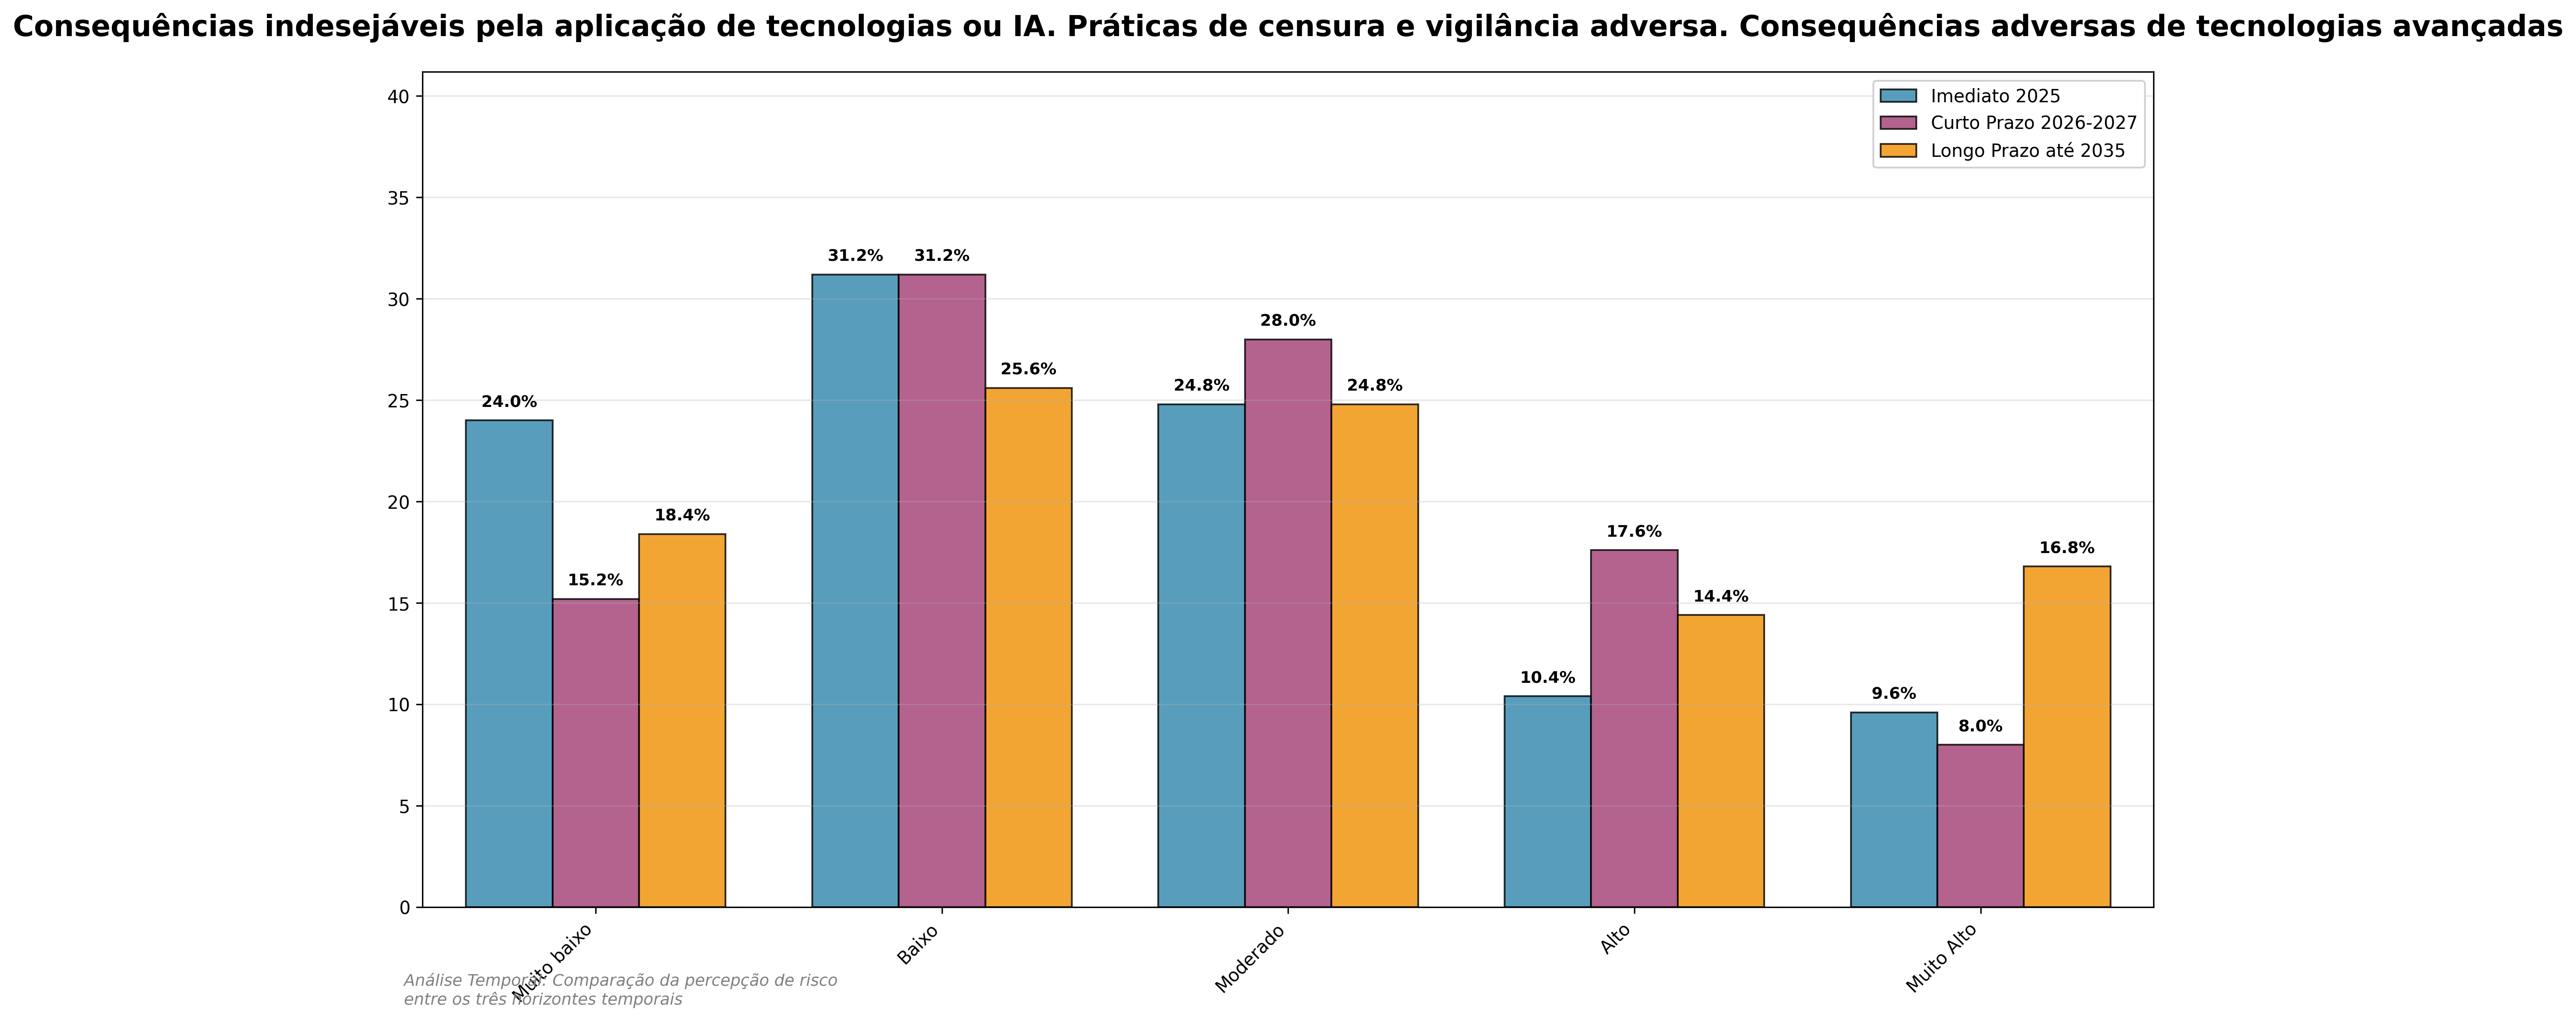
\includegraphics[keepaspectratio]{assets/tecnologicos/grafico_agrupado_5_8_temporal.png}}

\begin{tcolorbox}[enhanced jigsaw, titlerule=0mm, colback=white, title=\textcolor{quarto-callout-tip-color}{\faLightbulb}\hspace{0.5em}{Destaques}, opacityback=0, colbacktitle=quarto-callout-tip-color!10!white, leftrule=.75mm, left=2mm, colframe=quarto-callout-tip-color-frame, bottomrule=.15mm, bottomtitle=1mm, breakable, toprule=.15mm, toptitle=1mm, opacitybacktitle=0.6, arc=.35mm, coltitle=black, rightrule=.15mm]

\textbf{Imediato (2025)}: Mediana 2.0, 20\% em risco alto

\textbf{Curto Prazo (2026-2027)}: Mediana 3.0, 26\% em risco alto

\textbf{Longo Prazo (até 2035)}: Mediana 3.0, 31\% em risco alto

\begin{itemize}
\tightlist
\item
  \textbf{Tendência}: Percepção de risco relativamente estável ao longo
  do tempo. \textbf{Análise - Consequências indesejáveis pela aplicação
  de tecnologias ou IA (censura e vigilância)} \textbf{Imediato (2025)}:
  Devido a consequências iniciais pela aplicação de tecnologias ou IA,
  como práticas pontuais de censura e vigilância, poderá acontecer o uso
  limitado e controlado dessas tecnologias no ambiente portuário
  brasileiro, o que poderá levar a impactos restritos na privacidade e
  na liberdade de informação, impactando minimamente os direitos dos
  trabalhadores e a reputação do setor.
\end{itemize}

\textbf{Curto prazo (2026-2027)}: Devido a consequências indesejáveis
pela aplicação de tecnologias ou IA, como práticas moderadas de censura
e vigilância no ambiente portuário, poderá acontecer o uso inadequado de
sistemas automatizados para monitoramento de trabalhadores e operações,
o que poderá levar a restrições parciais na privacidade e no acesso à
informação, impactando nos direitos laborais e na confiança
institucional do setor portuário brasileiro no curto prazo (2026 a
2027).

\textbf{Longo prazo (até 2035)}: Devido a consequências indesejáveis
pela aplicação de tecnologias ou IA, como práticas moderadas de censura
e vigilância, poderá acontecer o uso inadequado de ferramentas digitais
no ambiente portuário brasileiro, o que poderá levar a restrições
parciais na privacidade e no acesso à informação, impactando de forma
moderada os direitos dos trabalhadores e a imagem do setor no longo
prazo.

\end{tcolorbox}

\subsection{Riscos associados à introdução de navios
autônomos}\label{riscos-associados-uxe0-introduuxe7uxe3o-de-navios-autuxf4nomos}

O gr?fico a seguir apresenta a evolu??o temporal do risco Riscos
associados à introdução de navios autônomos.
\pandocbounded{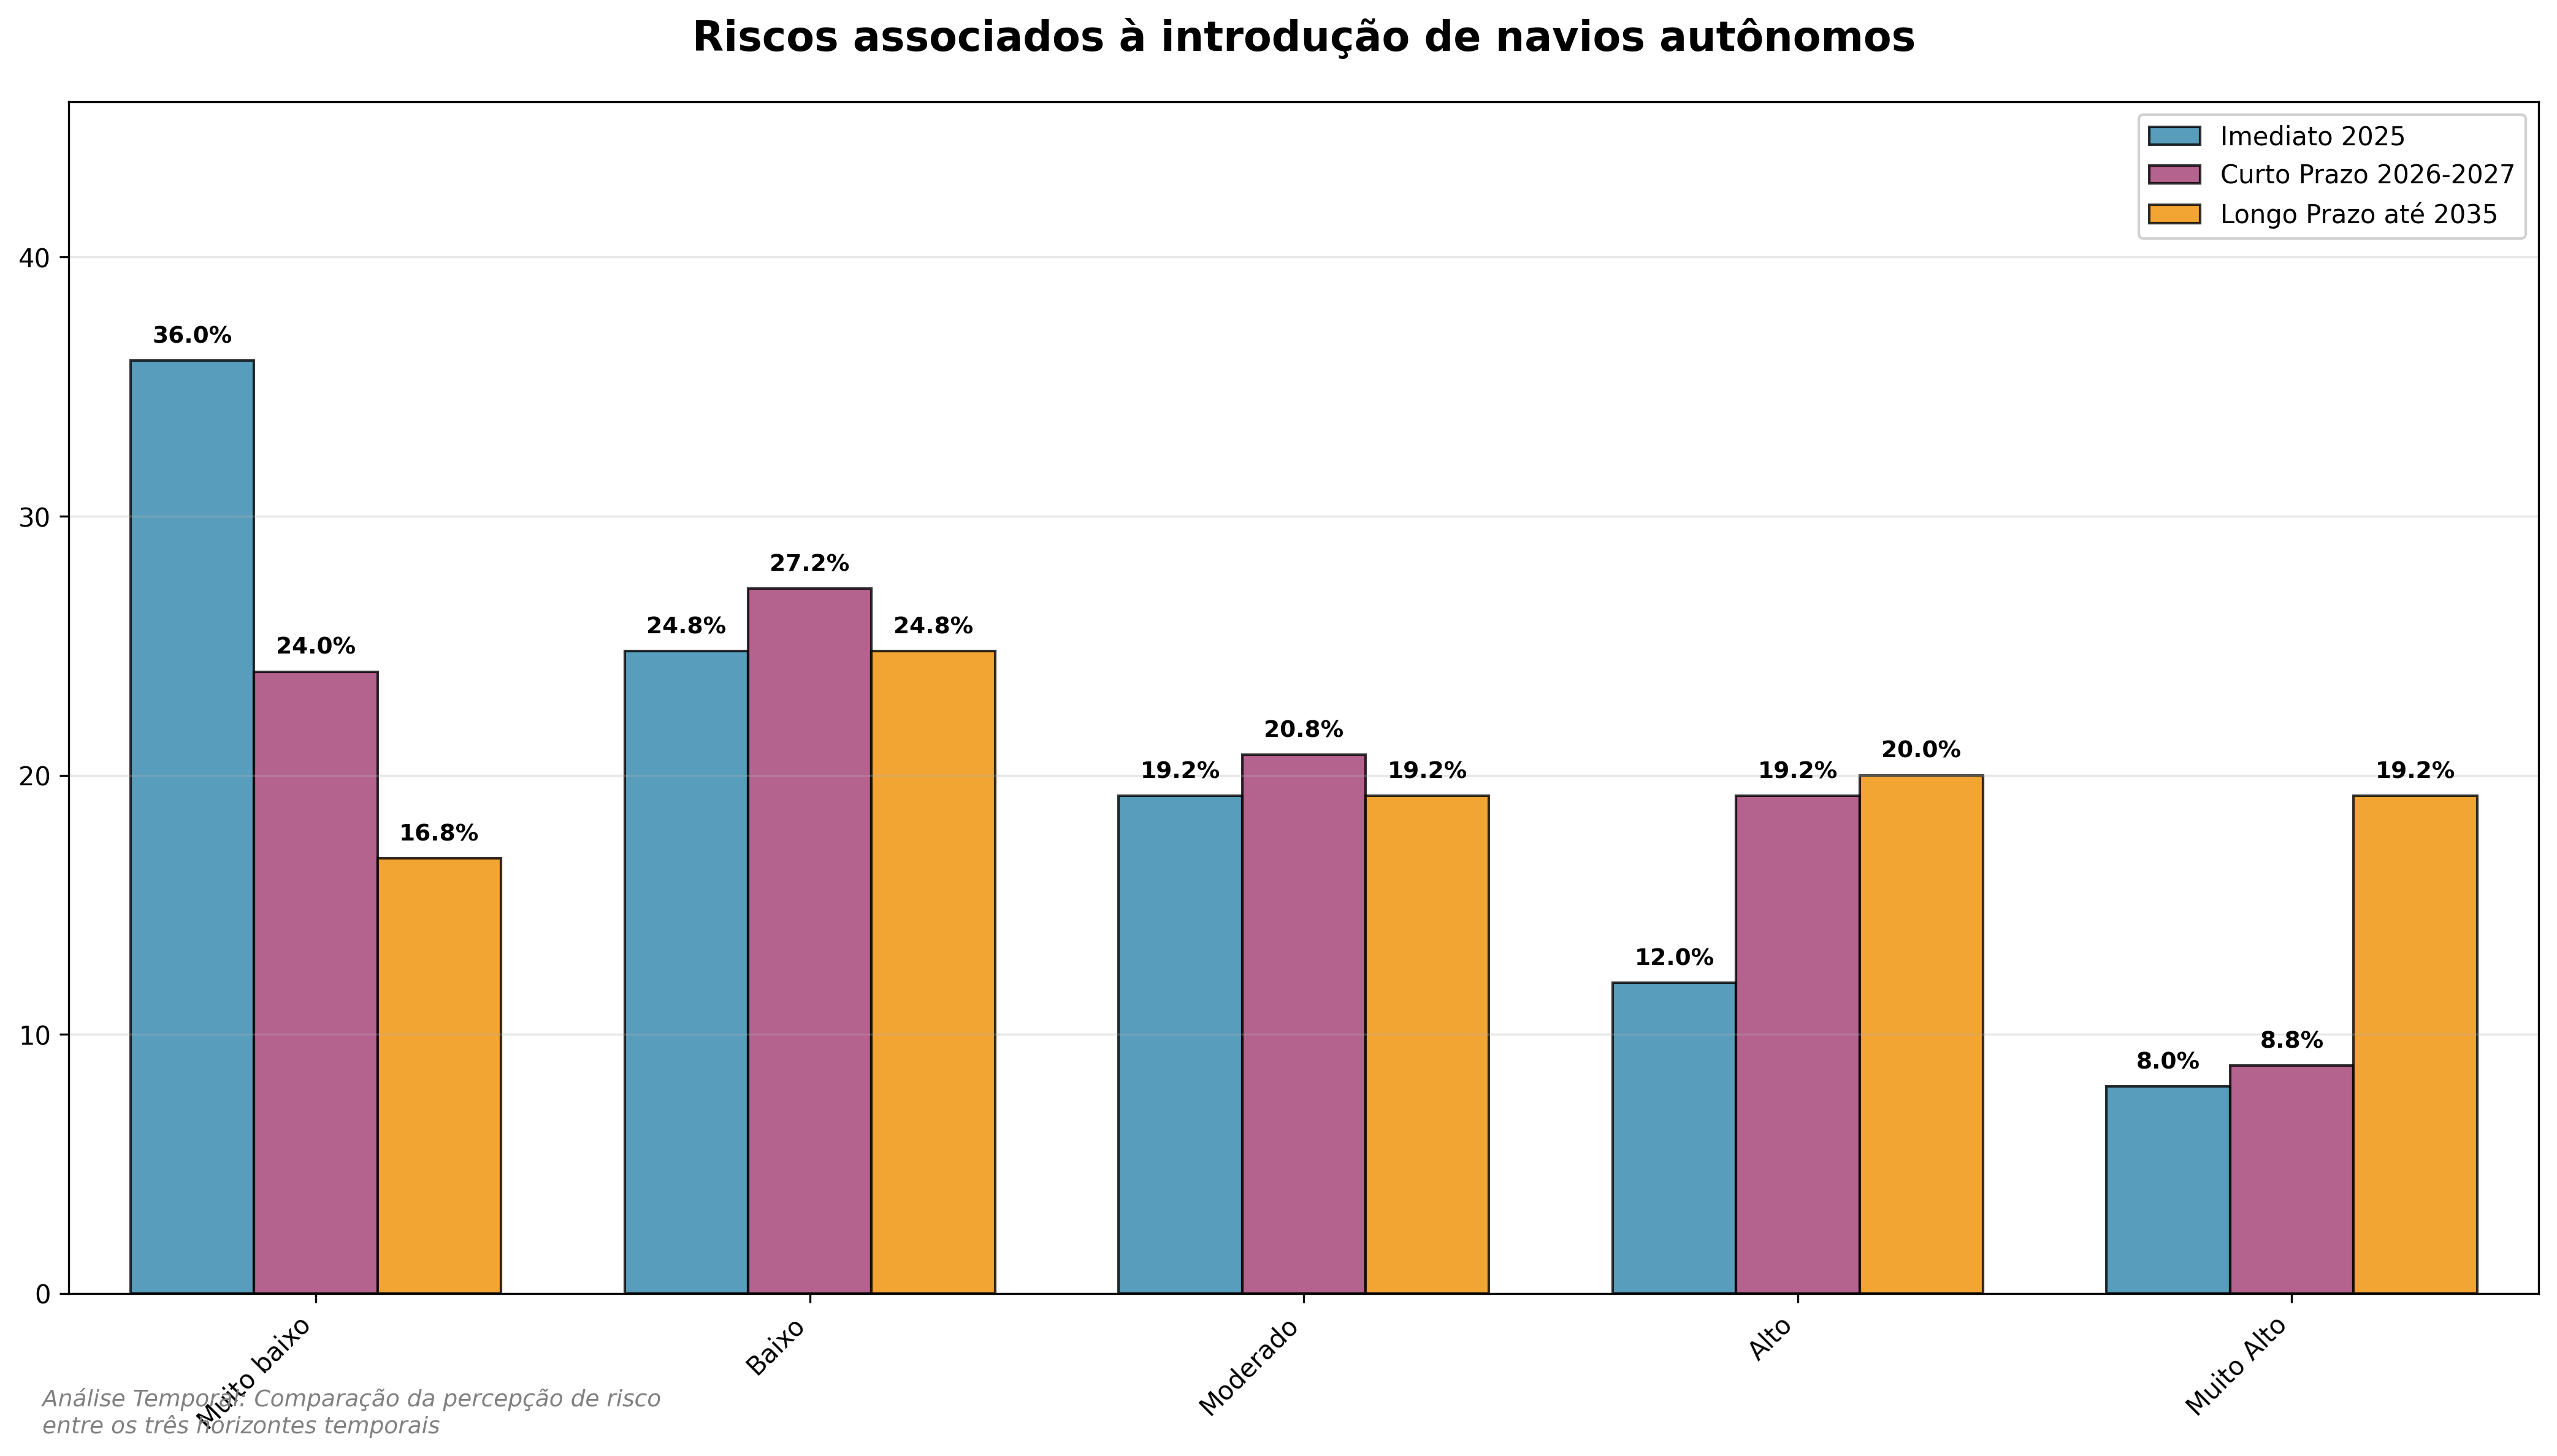
\includegraphics[keepaspectratio]{assets/tecnologicos/grafico_agrupado_5_9_temporal.png}}

\begin{tcolorbox}[enhanced jigsaw, titlerule=0mm, colback=white, title=\textcolor{quarto-callout-tip-color}{\faLightbulb}\hspace{0.5em}{Destaques}, opacityback=0, colbacktitle=quarto-callout-tip-color!10!white, leftrule=.75mm, left=2mm, colframe=quarto-callout-tip-color-frame, bottomrule=.15mm, bottomtitle=1mm, breakable, toprule=.15mm, toptitle=1mm, opacitybacktitle=0.6, arc=.35mm, coltitle=black, rightrule=.15mm]

\textbf{Imediato (2025)}: Mediana 2.0, 20\% em risco alto

\textbf{Curto Prazo (2026-2027)}: Mediana 2.0, 28\% em risco alto

\textbf{Longo Prazo (até 2035)}: Mediana 3.0, 39\% em risco alto

\textbf{Análise - Riscos associados à introdução de navios autônomos}
\textbf{Imediato (2025)}: Devido à introdução inicial de navios
autônomos no setor portuário brasileiro, poderá acontecer o surgimento
de algumas novas categorias de ameaças tecnológicas e operacionais ainda
pouco exploradas, o que poderá levar a vulnerabilidades cibernéticas e
falhas pontuais em sistemas de inteligência artificial, impactando de
forma limitada a segurança da navegação e a governança do setor.

\textbf{Curto prazo (2026-2027)}: Devido à introdução inicial de navios
autônomos no setor portuário brasileiro, poderá acontecer o surgimento
de algumas novas categorias de ameaças tecnológicas e operacionais ainda
pouco expressivas, o que poderá levar a vulnerabilidades cibernéticas e
falhas pontuais em sistemas de inteligência artificial, impactando de
forma limitada a segurança da navegação e a governança do setor.

\textbf{Longo prazo (até 2035)}: Devido à crescente incorporação de
navios autônomos no setor portuário brasileiro até 2035, poderá
acontecer a manifestação de novas categorias de riscos tecnológicos,
operacionais e regulatórios, o que poderá levar a desafios moderados em
vulnerabilidades cibernéticas e eventuais falhas em sistemas de
inteligência artificial, impactando a segurança da navegação e a
eficiência da governança portuária, demandando monitoramento constante e
estratégias de gestão adequadas.

\end{tcolorbox}

\subsection{Riscos associados às tecnologias
espaciais}\label{riscos-associados-uxe0s-tecnologias-espaciais}

O gr?fico a seguir apresenta a evolu??o temporal do risco Riscos
associados às tecnologias espaciais.
\pandocbounded{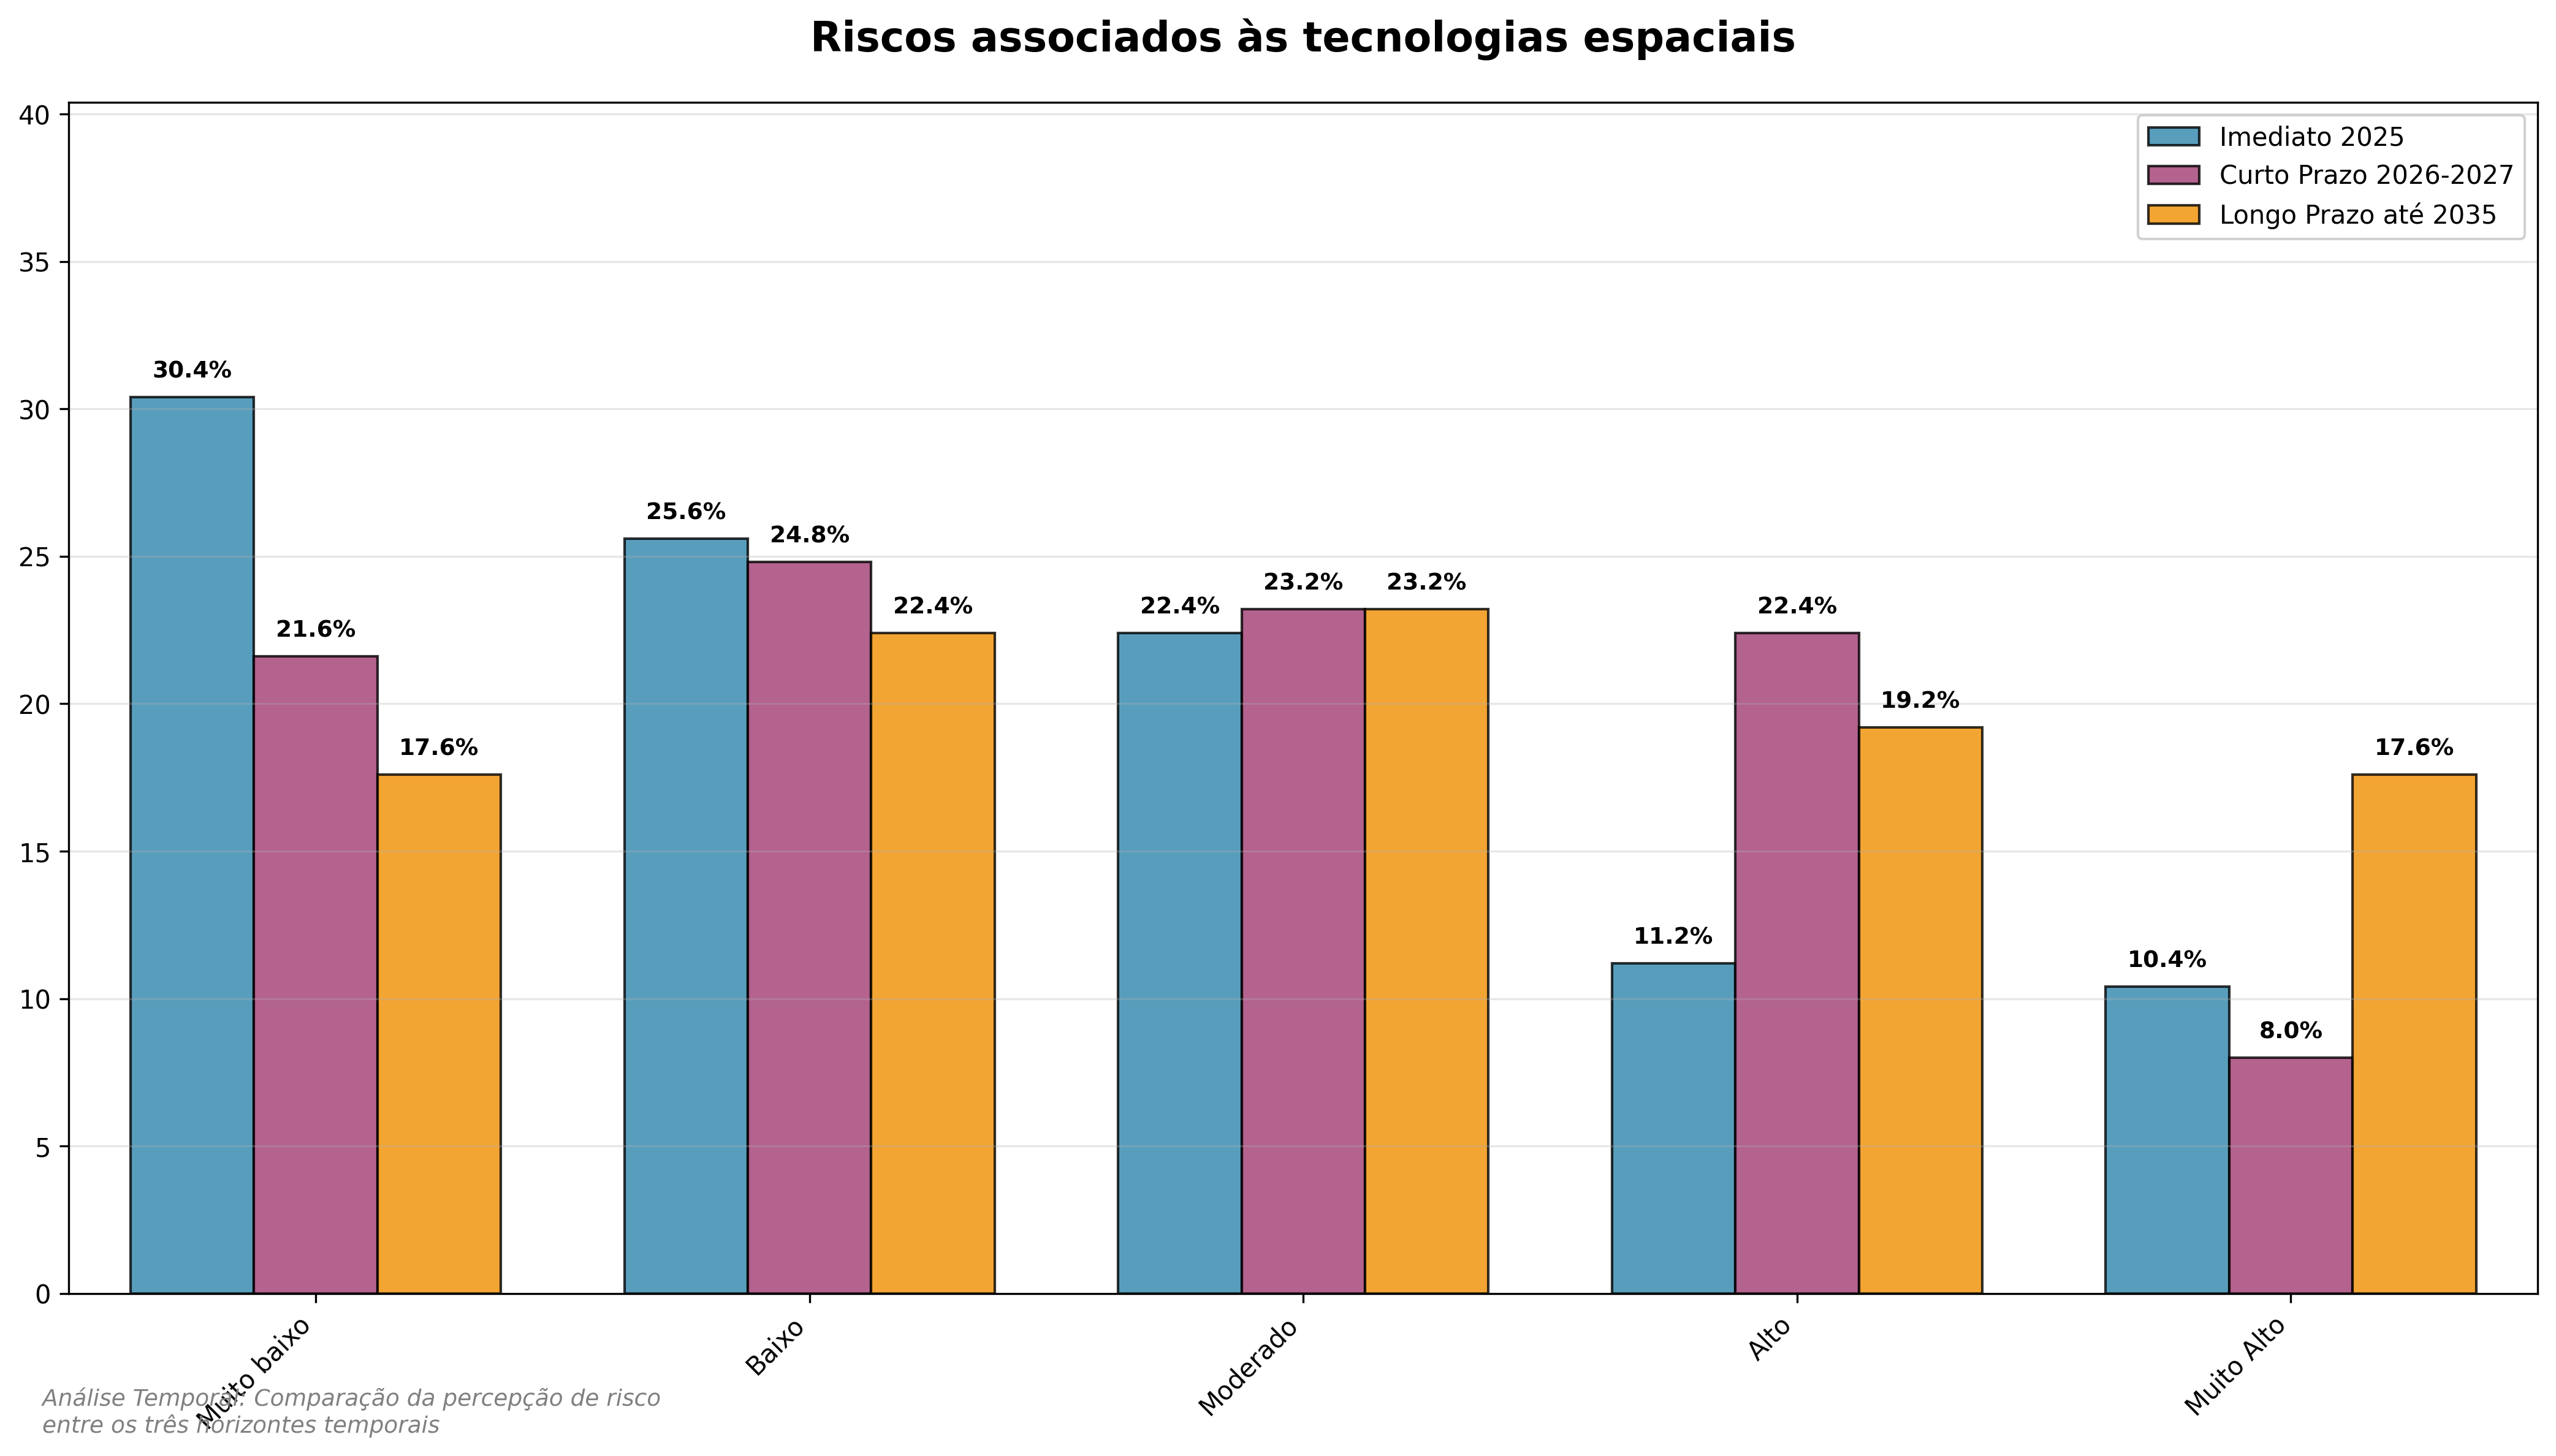
\includegraphics[keepaspectratio]{assets/tecnologicos/grafico_agrupado_5_10_temporal.png}}

\begin{tcolorbox}[enhanced jigsaw, titlerule=0mm, colback=white, title=\textcolor{quarto-callout-tip-color}{\faLightbulb}\hspace{0.5em}{Destaques}, opacityback=0, colbacktitle=quarto-callout-tip-color!10!white, leftrule=.75mm, left=2mm, colframe=quarto-callout-tip-color-frame, bottomrule=.15mm, bottomtitle=1mm, breakable, toprule=.15mm, toptitle=1mm, opacitybacktitle=0.6, arc=.35mm, coltitle=black, rightrule=.15mm]

\textbf{Imediato (2025)}: Mediana 2.0, 22\% em risco alto

\textbf{Curto Prazo (2026-2027)}: Mediana 3.0, 30\% em risco alto

\textbf{Longo Prazo (até 2035)}: Mediana 3.0, 37\% em risco alto

\textbf{Análise - Riscos associados às tecnologias espaciais}
\textbf{Imediato (2025)}: Devido aos riscos iniciais associados às
tecnologias espaciais, poderá acontecer a exposição pontual das cadeias
logísticas portuárias brasileiras a vulnerabilidades como falhas
temporárias de sinal, o que poderá levar a pequenas interrupções
operacionais localizadas, impactando de forma limitada a segurança e a
continuidade do comércio exterior.

\textbf{Curto prazo (2026-2027)}: Devido aos riscos associados às
tecnologias espaciais, poderá acontecer a exposição das cadeias
logísticas portuárias brasileiras a vulnerabilidades como instabilidades
temporárias de sinal ou tentativas de interferência cibernética, o que
poderá levar a interrupções pontuais nas operações e na coordenação
logística, impactando na eficiência operacional e na continuidade do
comércio exterior.

\textbf{Longo prazo (até 2035)}: Devido aos riscos associados às
tecnologias espaciais, poderá acontecer a exposição das cadeias
logísticas portuárias brasileiras a vulnerabilidades operacionais, como
falhas temporárias de sinal ou tentativas de interferência cibernética,
o que poderá levar a interrupções parciais nas operações e na
coordenação logística, impactando na segurança e continuidade do
comércio exterior de forma moderada e exigindo monitoramento constante e
medidas de mitigação adequadas.

\end{tcolorbox}

\subsection{Riscos associados à automação
portuária}\label{riscos-associados-uxe0-automauxe7uxe3o-portuuxe1ria}

O gr?fico a seguir apresenta a evolu??o temporal do risco Riscos
associados à automação portuária.
\pandocbounded{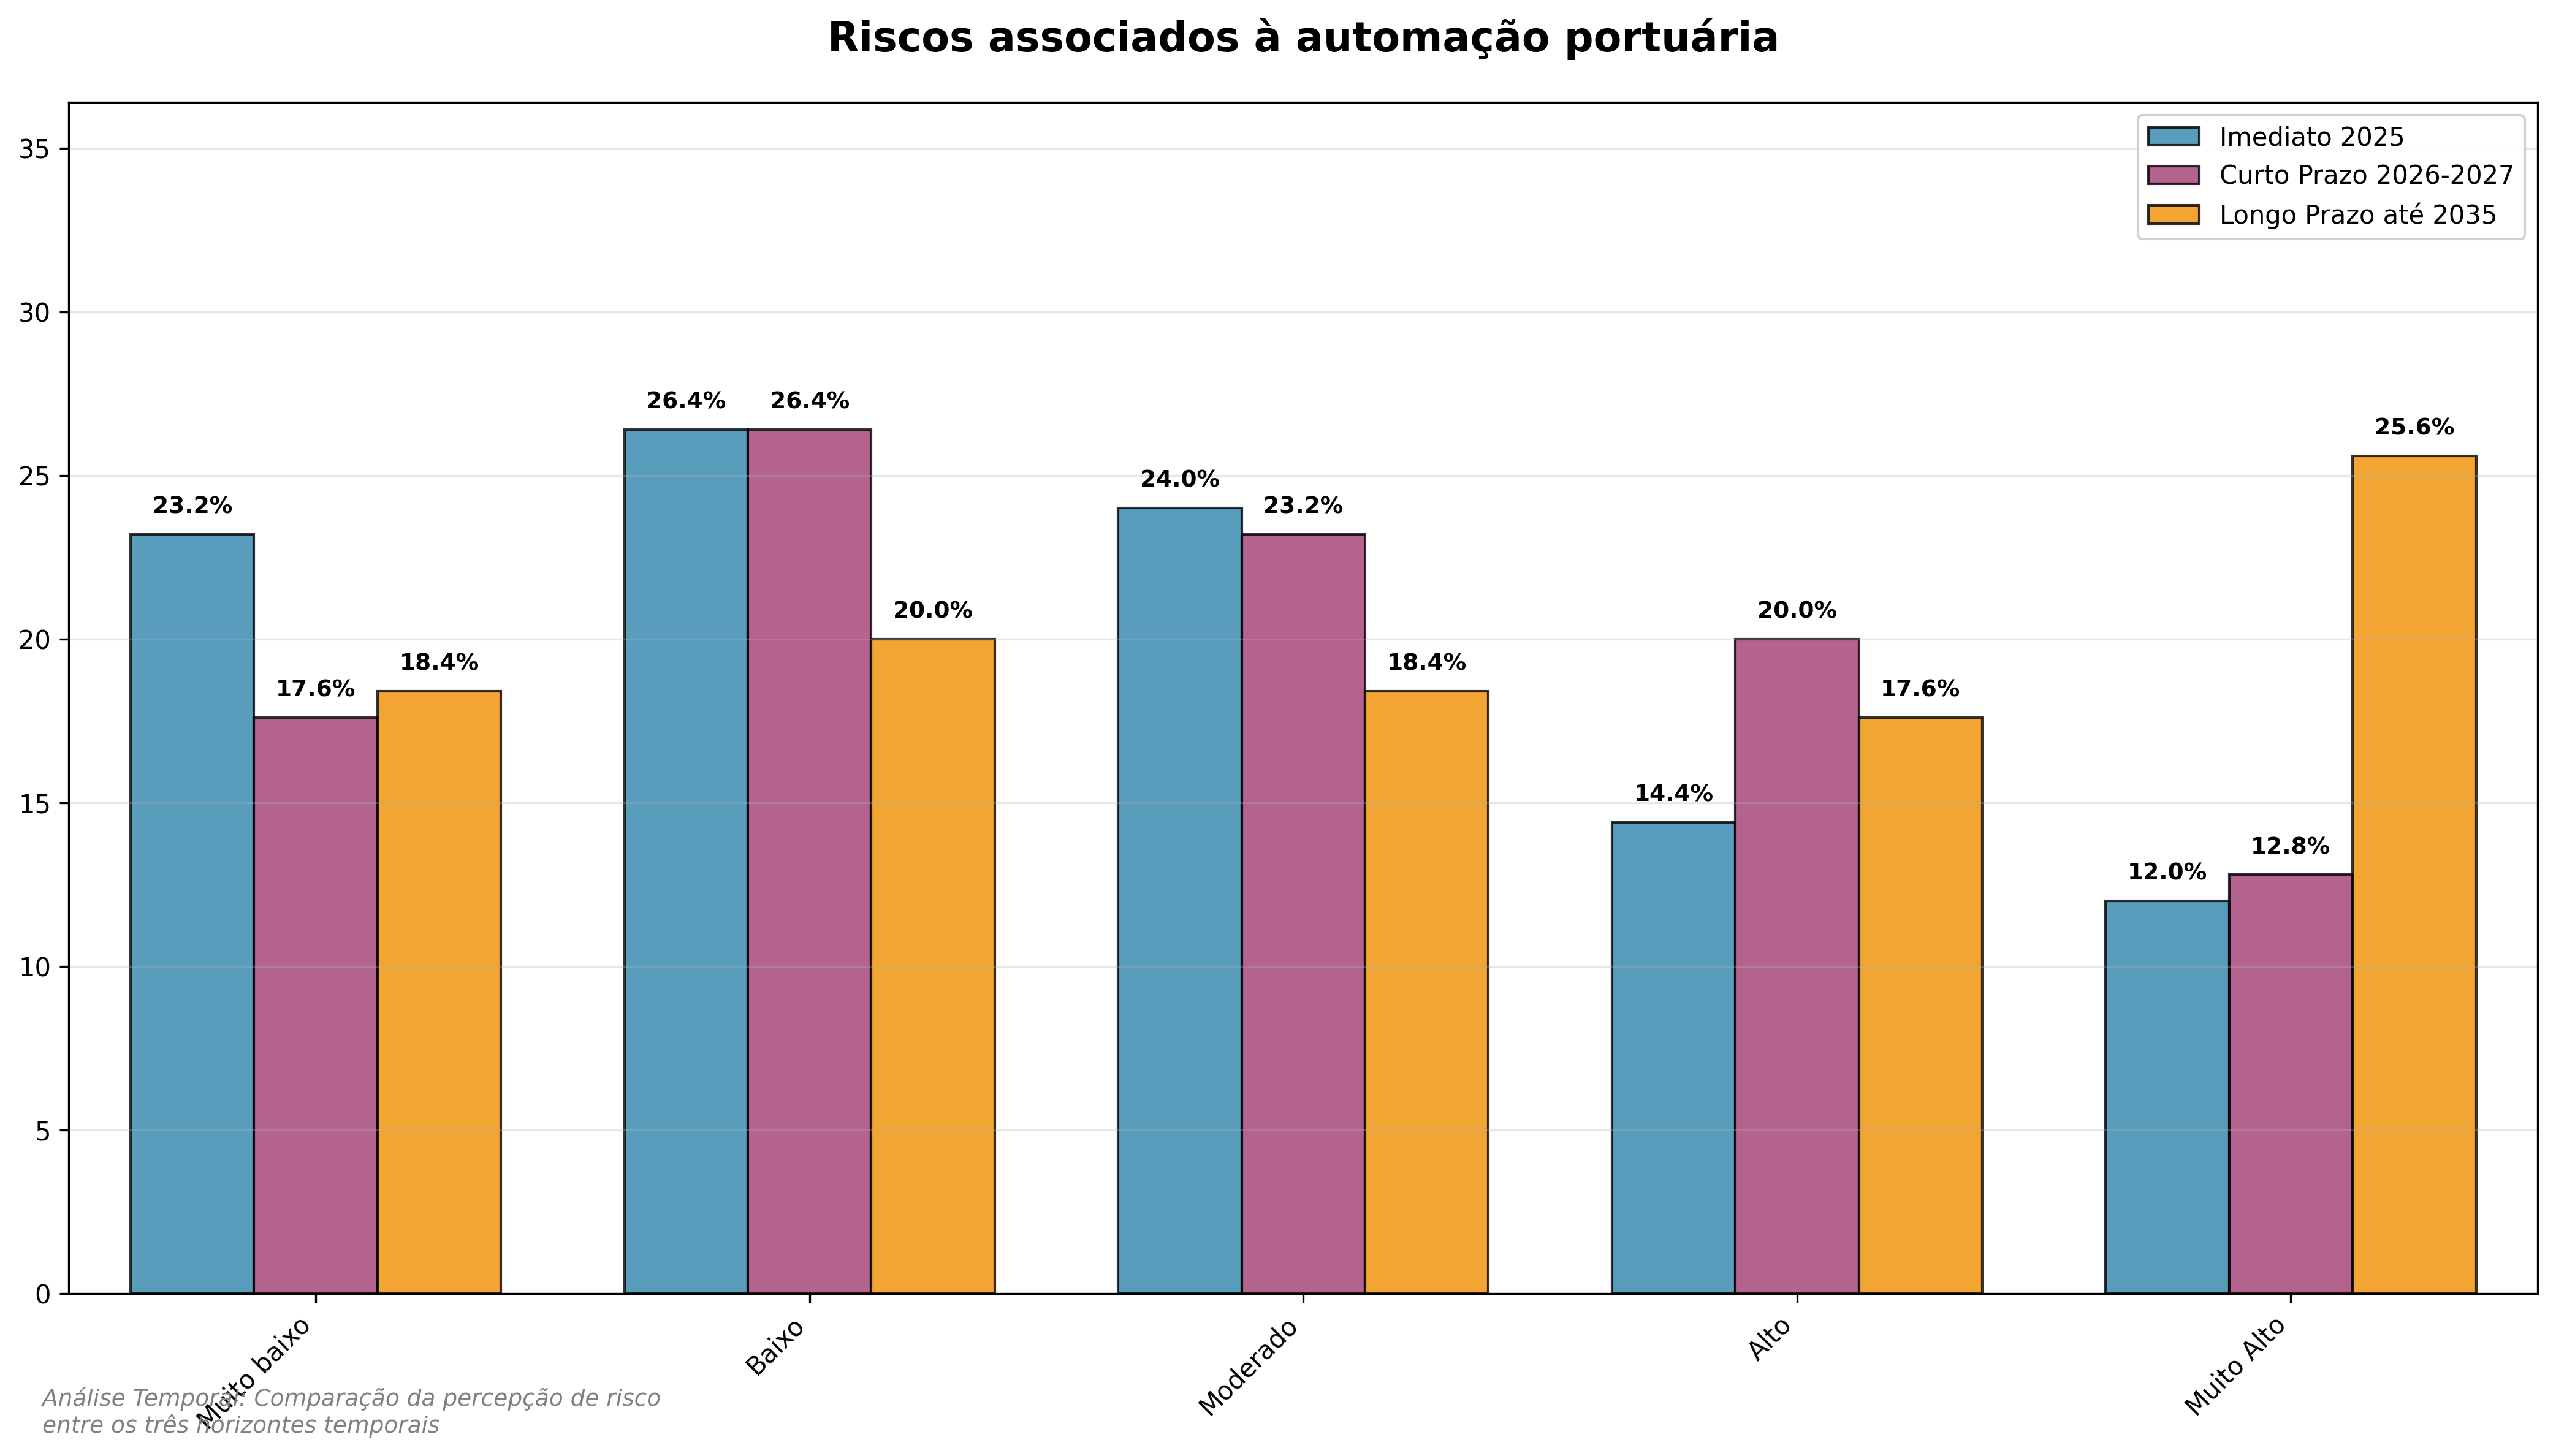
\includegraphics[keepaspectratio]{assets/tecnologicos/grafico_agrupado_5_11_temporal.png}}

\begin{tcolorbox}[enhanced jigsaw, titlerule=0mm, colback=white, title=\textcolor{quarto-callout-tip-color}{\faLightbulb}\hspace{0.5em}{Destaques}, opacityback=0, colbacktitle=quarto-callout-tip-color!10!white, leftrule=.75mm, left=2mm, colframe=quarto-callout-tip-color-frame, bottomrule=.15mm, bottomtitle=1mm, breakable, toprule=.15mm, toptitle=1mm, opacitybacktitle=0.6, arc=.35mm, coltitle=black, rightrule=.15mm]

\textbf{Imediato (2025)}: Mediana 3.0, 26\% em risco alto

\textbf{Curto Prazo (2026-2027)}: Mediana 3.0, 33\% em risco alto

\textbf{Longo Prazo (até 2035)}: Mediana 3.0, 43\% em risco alto

\textbf{Análise - Riscos associados à automação portuária}
\textbf{Imediato (2025)}: Devido à crescente adoção da automação nos
portos brasileiros, poderá acontecer a manifestação de vulnerabilidades
cibernéticas e falhas operacionais pontuais, bem como maior dependência
de sistemas tecnológicos específicos, o que poderá levar a interrupções
moderadas nas operações e a desafios na gestão da continuidade dos
processos logísticos, impactando a eficiência e a confiabilidade das
cadeias de suprimentos no curto prazo.

\textbf{Curto prazo (2026-2027)}: Devido à crescente automação nos
portos brasileiros, poderá acontecer a exposição moderada do setor a
vulnerabilidades cibernéticas e falhas sistêmicas pontuais, além de uma
dependência tecnológica em desenvolvimento, o que poderá levar a
interrupções operacionais localizadas e atrasos nas cadeias logísticas,
impactando a eficiência das operações portuárias no curto prazo.

\textbf{Longo prazo (até 2035)}: Devido à crescente adoção da automação
nos portos brasileiros, poderá acontecer a exposição do setor a
vulnerabilidades cibernéticas e falhas operacionais pontuais, além da
dependência crescente de sistemas tecnológicos, o que poderá levar a
interrupções moderadas nas operações portuárias e afetar a eficiência
das cadeias logísticas nacionais e internacionais.

\end{tcolorbox}

\subsection{Problemas de integração de
segurança}\label{problemas-de-integrauxe7uxe3o-de-seguranuxe7a}

O gr?fico a seguir apresenta a evolu??o temporal do risco Problemas de
integração de segurança.
\pandocbounded{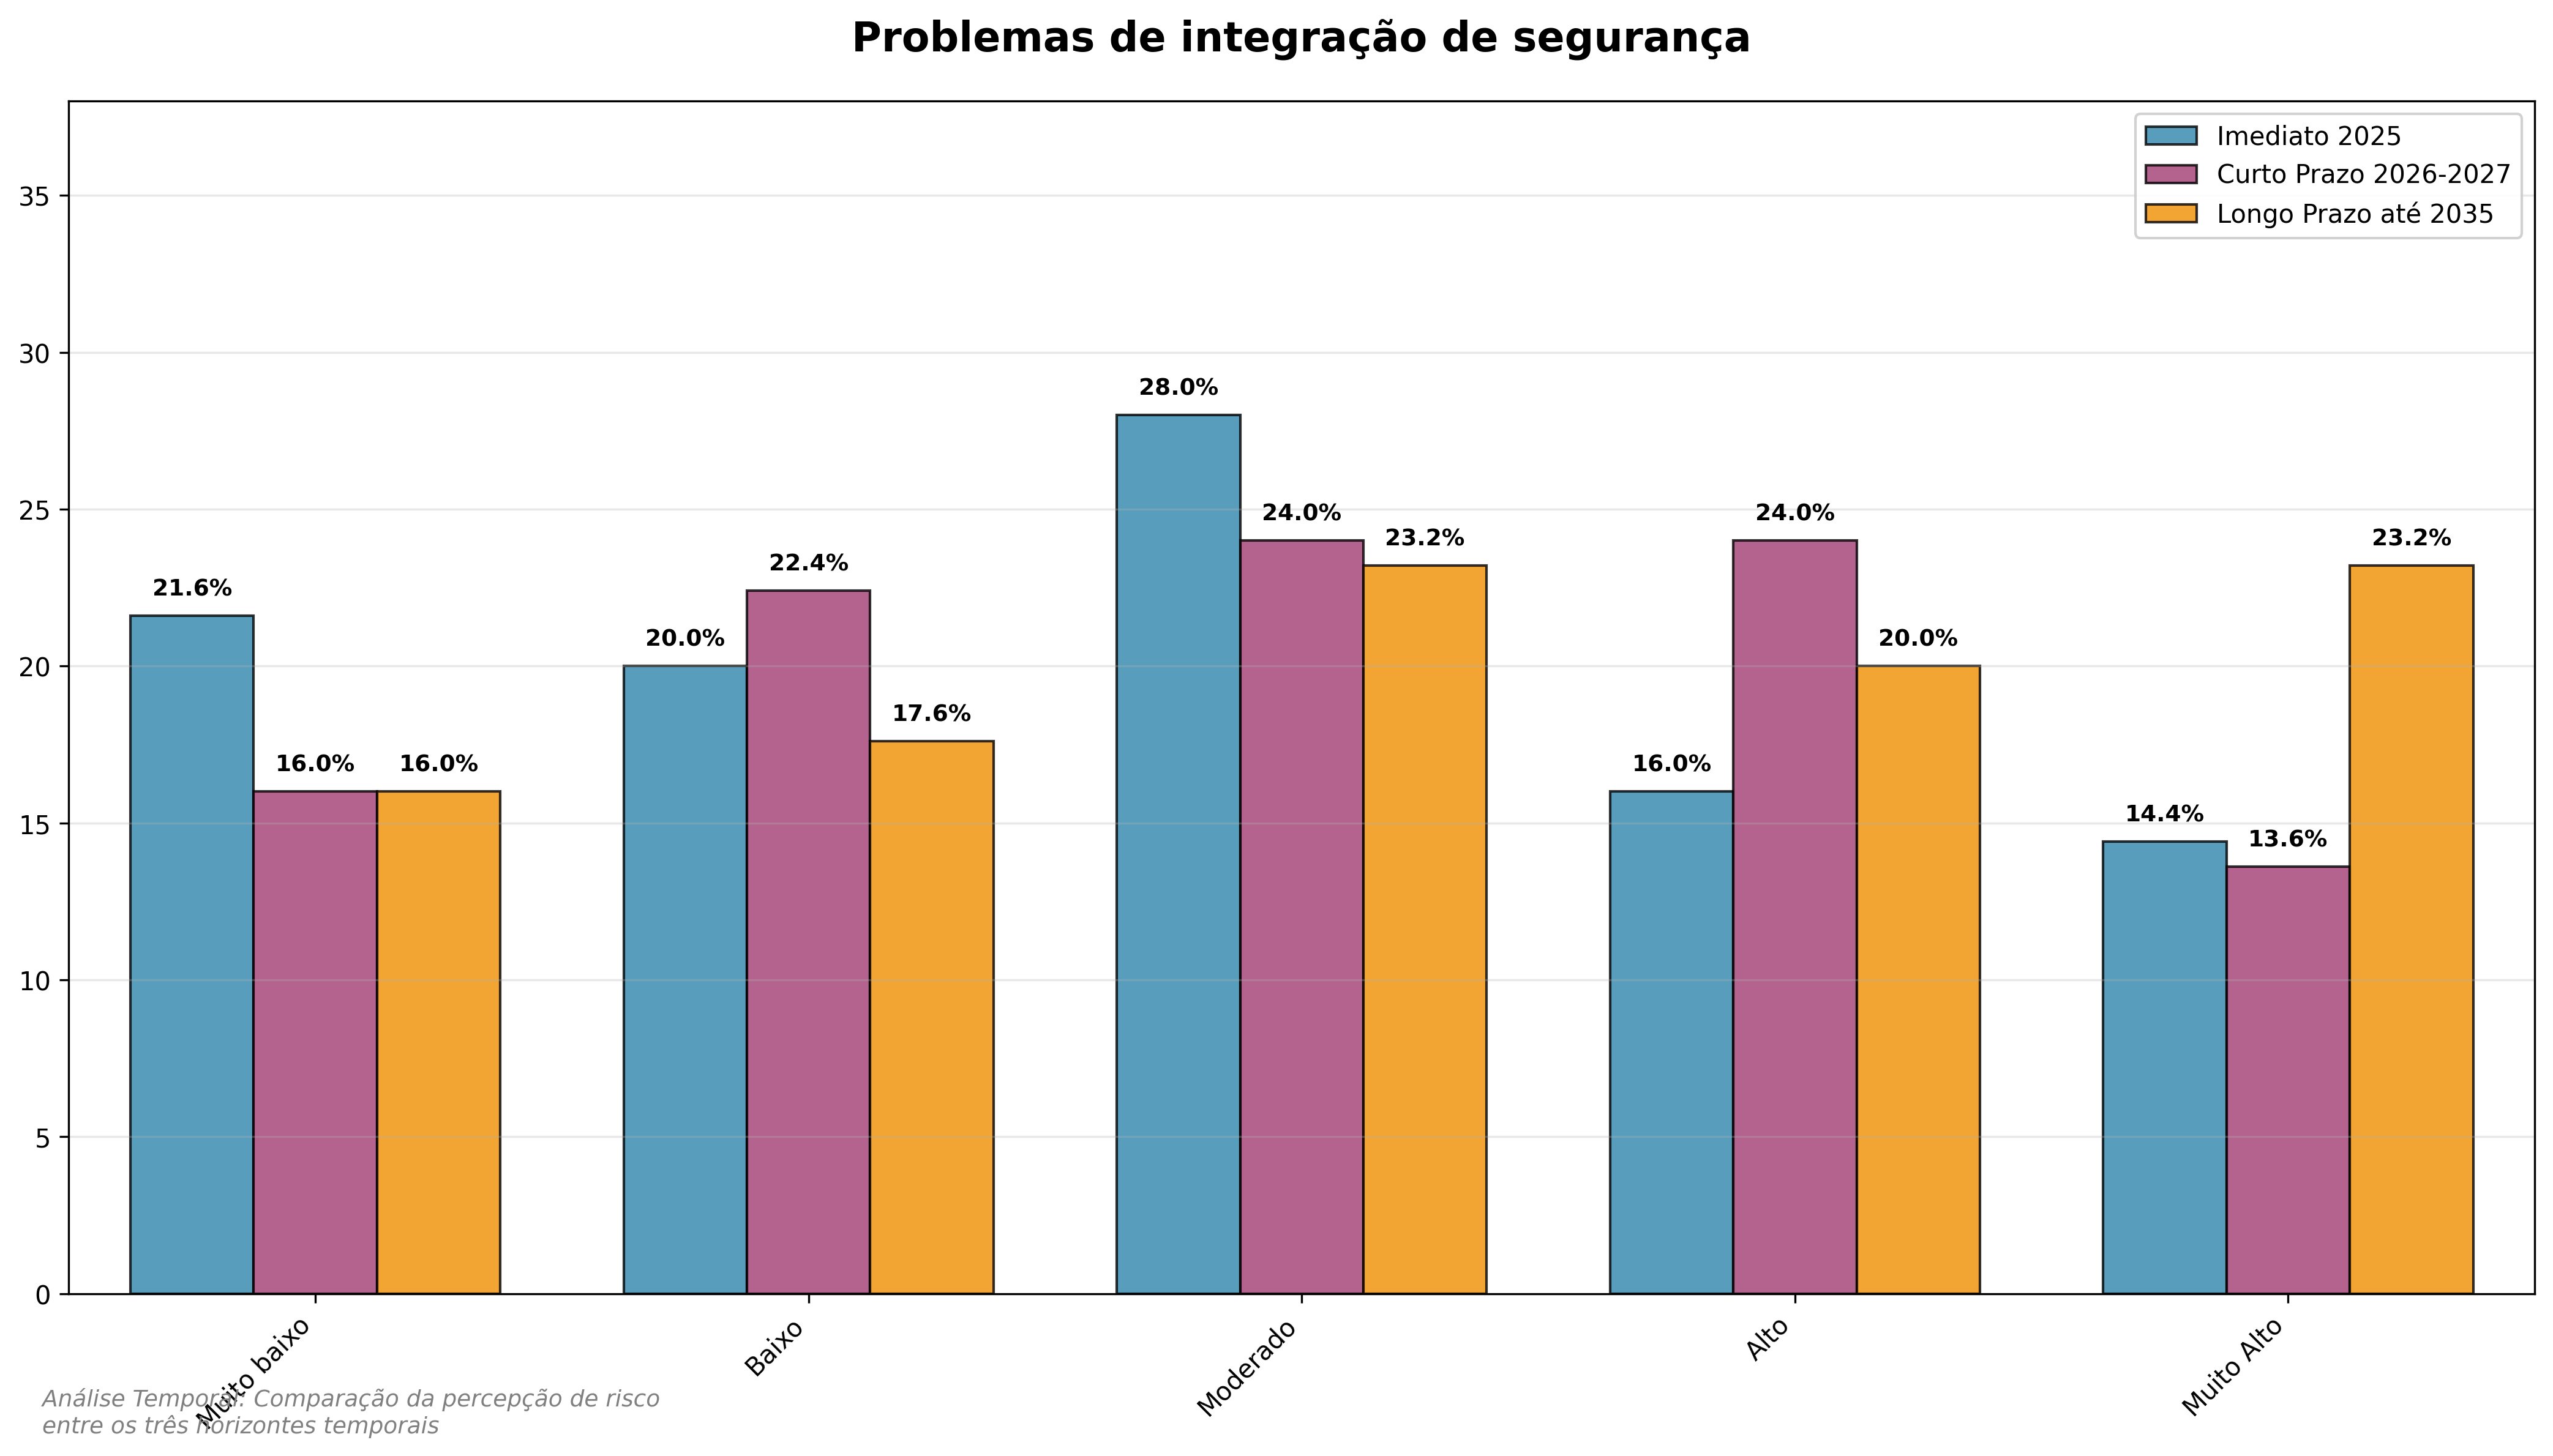
\includegraphics[keepaspectratio]{assets/tecnologicos/grafico_agrupado_5_12_temporal.png}}

\begin{tcolorbox}[enhanced jigsaw, titlerule=0mm, colback=white, title=\textcolor{quarto-callout-tip-color}{\faLightbulb}\hspace{0.5em}{Destaques}, opacityback=0, colbacktitle=quarto-callout-tip-color!10!white, leftrule=.75mm, left=2mm, colframe=quarto-callout-tip-color-frame, bottomrule=.15mm, bottomtitle=1mm, breakable, toprule=.15mm, toptitle=1mm, opacitybacktitle=0.6, arc=.35mm, coltitle=black, rightrule=.15mm]

\textbf{Imediato (2025)}: Mediana 3.0, 30\% em risco alto

\textbf{Curto Prazo (2026-2027)}: Mediana 3.0, 38\% em risco alto

\textbf{Longo Prazo (até 2035)}: Mediana 3.0, 43\% em risco alto

\textbf{Análise - Problemas de integração de segurança} \textbf{Imediato
(2025)}: Devido a desafios na integração de segurança entre sistemas e
agentes portuários, poderá acontecer a ocorrência de falhas pontuais na
coordenação da vigilância e na resposta a incidentes, o que poderá levar
a vulnerabilidades moderadas frente a ataques cibernéticos e falhas
operacionais, impactando na eficiência das operações e exigindo
aprimoramento nos protocolos de gestão e comunicação.

\textbf{Curto prazo (2026-2027)}: Devido a desafios moderados na
integração de sistemas de segurança e na coordenação entre os diversos
agentes portuários brasileiros, poderá acontecer a ocorrência de falhas
pontuais na vigilância e respostas descoordenadas a incidentes, o que
poderá levar a uma vulnerabilidade controlada frente a ataques
cibernéticos, sabotagens ou erros operacionais, impactando de forma
moderada a continuidade das operações e a confiança dos stakeholders no
curto prazo (2026 a 2027).

\textbf{Longo prazo (até 2035)}: Devido a desafios persistentes na
integração de segurança entre sistemas e atores portuários, poderá
acontecer a ocorrência de lacunas pontuais na vigilância e respostas
menos coordenadas a incidentes, o que poderá levar a uma vulnerabilidade
moderada a ataques cibernéticos, sabotagens ou falhas operacionais,
impactando na eficiência das operações e na percepção de segurança pelos
stakeholders ao longo do tempo.

\end{tcolorbox}

\subsection{Privacidade e conformidade
legal}\label{privacidade-e-conformidade-legal}

O gr?fico a seguir apresenta a evolu??o temporal do risco Privacidade e
conformidade legal.
\pandocbounded{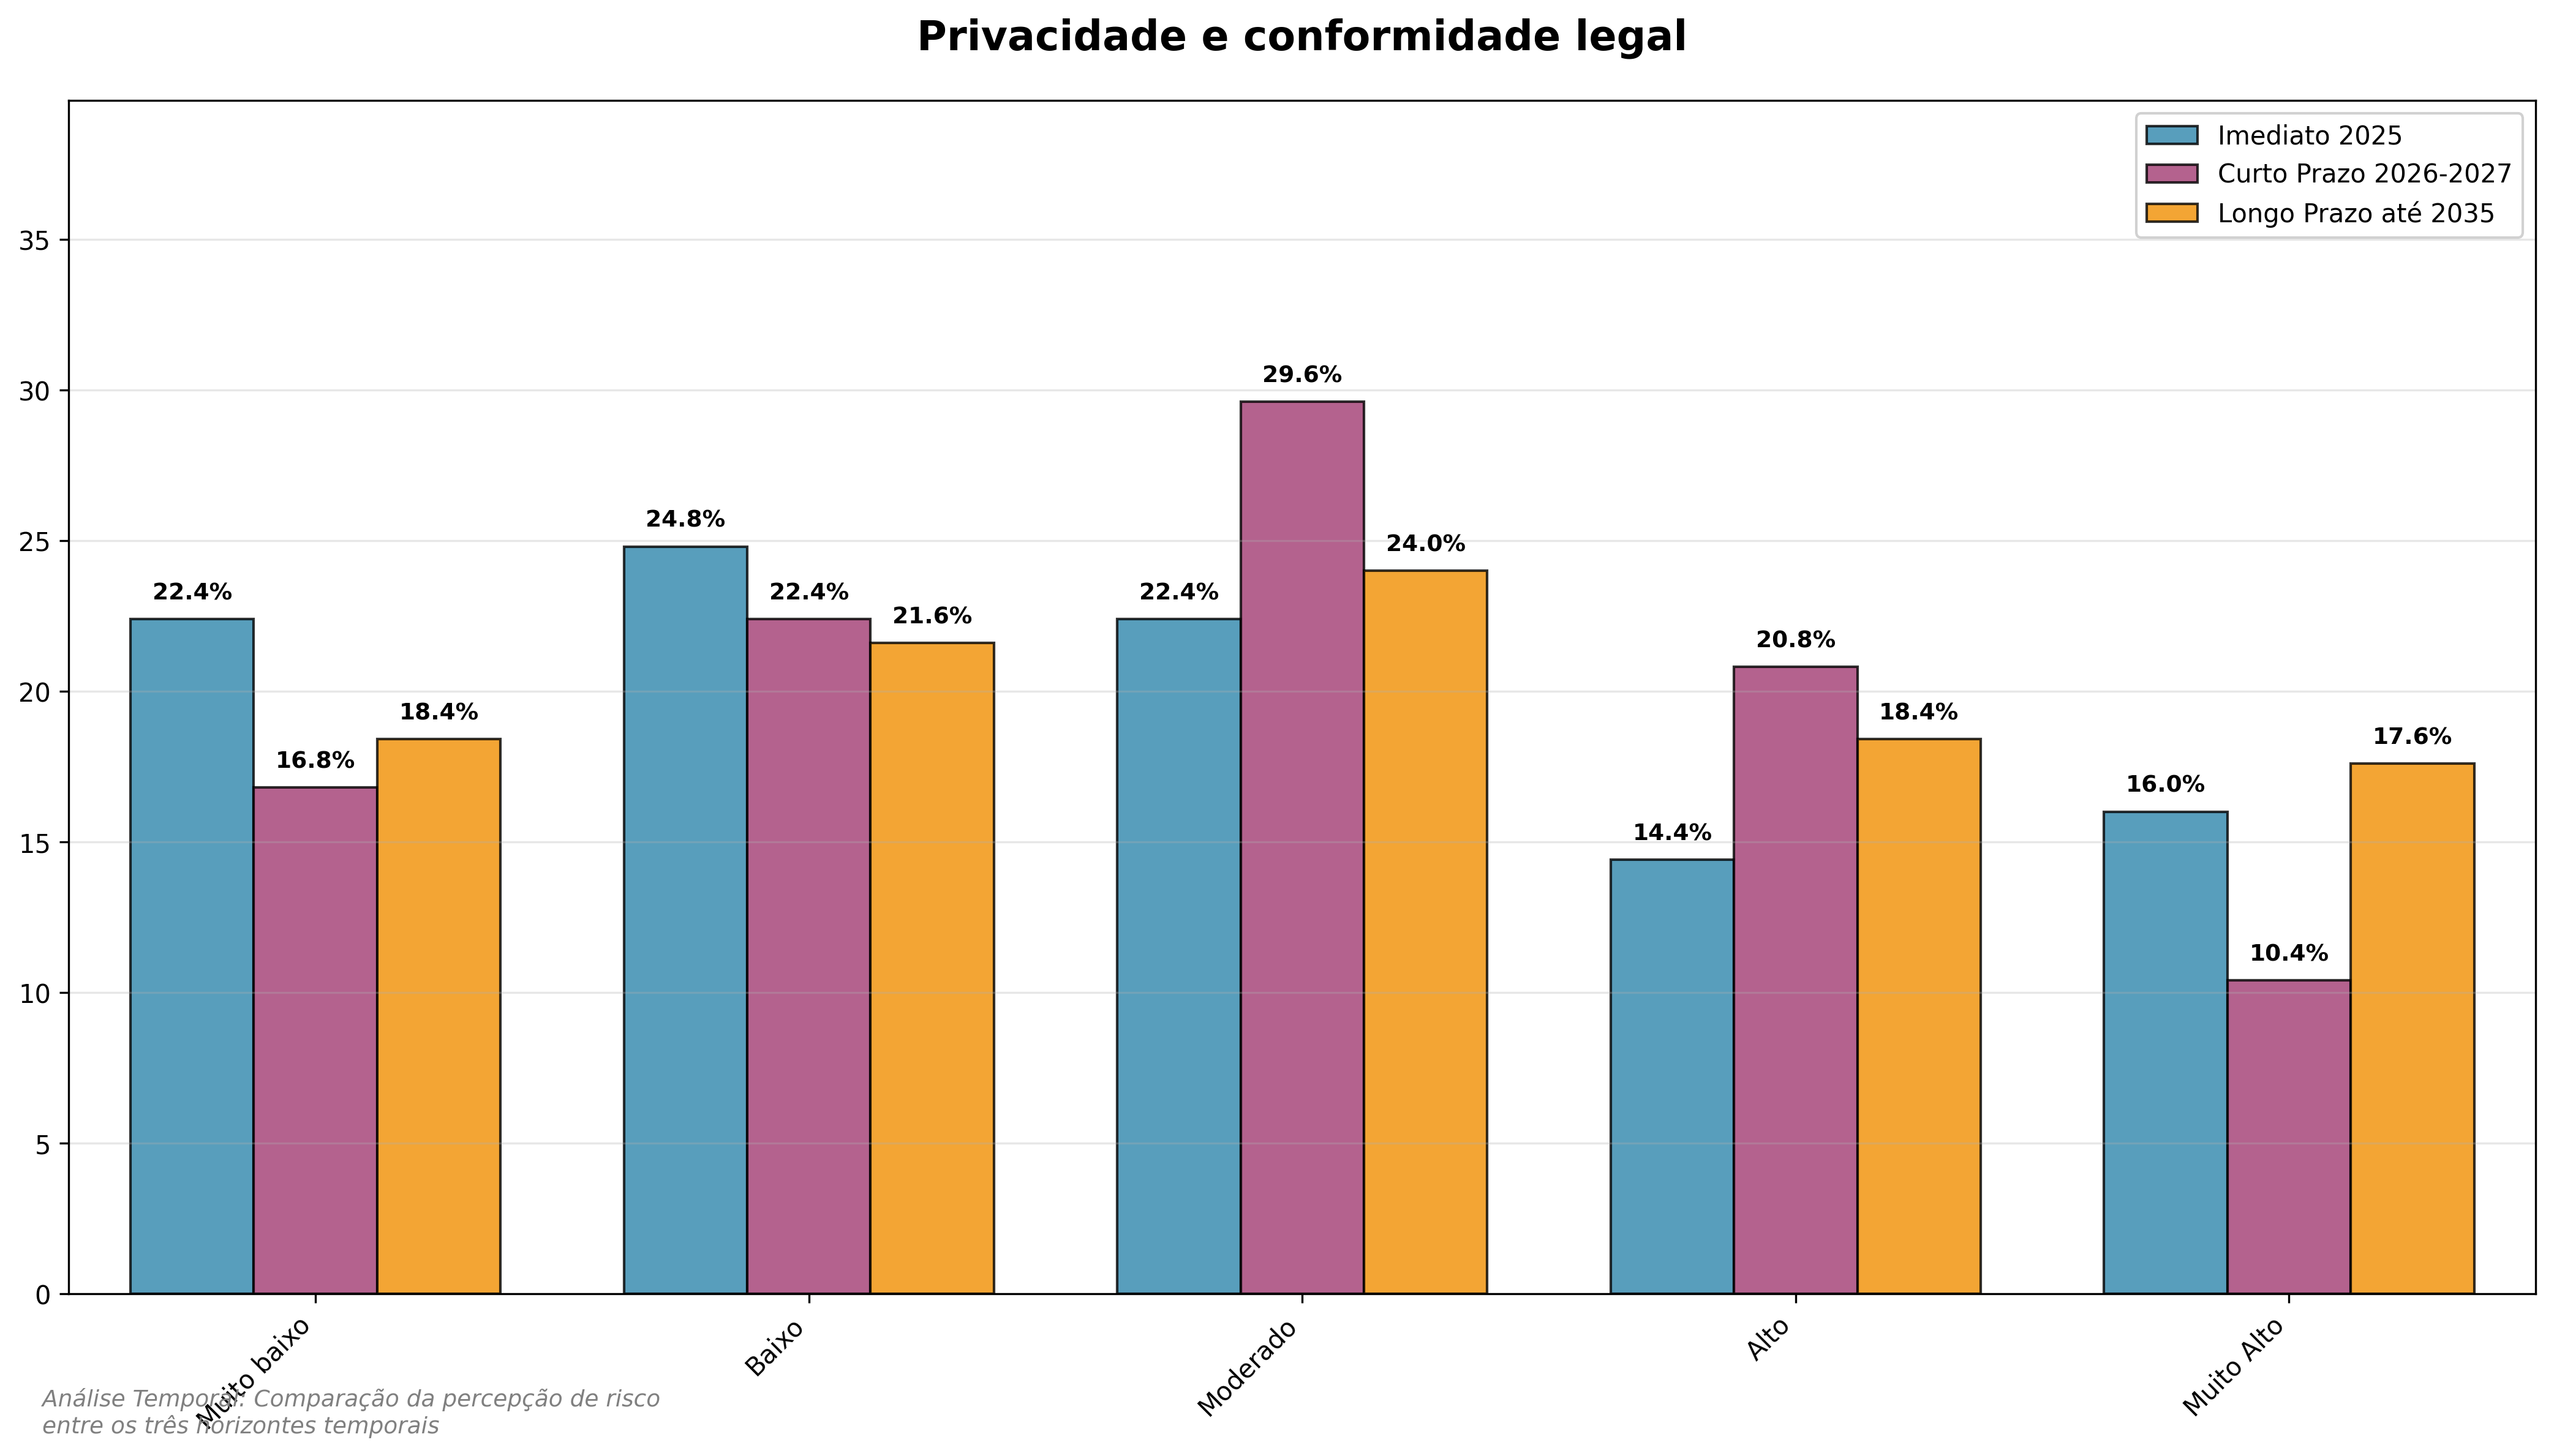
\includegraphics[keepaspectratio]{assets/tecnologicos/grafico_agrupado_5_13_temporal.png}}

\begin{tcolorbox}[enhanced jigsaw, titlerule=0mm, colback=white, title=\textcolor{quarto-callout-tip-color}{\faLightbulb}\hspace{0.5em}{Destaques}, opacityback=0, colbacktitle=quarto-callout-tip-color!10!white, leftrule=.75mm, left=2mm, colframe=quarto-callout-tip-color-frame, bottomrule=.15mm, bottomtitle=1mm, breakable, toprule=.15mm, toptitle=1mm, opacitybacktitle=0.6, arc=.35mm, coltitle=black, rightrule=.15mm]

\textbf{Imediato (2025)}: Mediana 3.0, 30\% em risco alto

\textbf{Curto Prazo (2026-2027)}: Mediana 3.0, 31\% em risco alto

\textbf{Longo Prazo (até 2035)}: Mediana 3.0, 36\% em risco alto

\textbf{Análise - Privacidade e conformidade legal} \textbf{Imediato
(2025)}: Devido a desafios na adequação contínua às normas de
privacidade e conformidade legal no tratamento de dados no setor
portuário brasileiro, poderá acontecer o descumprimento parcial de
requisitos regulatórios, o que poderá levar a sanções administrativas
moderadas, redução da confiança dos usuários e desgaste reputacional
pontual, impactando na segurança jurídica e na imagem do setor no
horizonte imediato.

\textbf{Curto prazo (2026-2027)}: Devido a desafios na adequação às
normas de privacidade e conformidade legal no tratamento de dados,
poderá acontecer a ocorrência de desvios pontuais em relação aos marcos
regulatórios vigentes, o que poderá levar a penalidades administrativas
moderadas, redução na confiança dos usuários e impactos reputacionais
localizados, impactando na segurança jurídica e na imagem do setor
portuário brasileiro no curto prazo.

\textbf{Longo prazo (até 2035)}: Devido à crescente complexidade das
normas de privacidade e conformidade legal no tratamento de dados no
setor portuário brasileiro, poderá acontecer a inadequação parcial aos
marcos regulatórios vigentes e emergentes, o que poderá levar a sanções
administrativas moderadas, perda gradual de confiança dos usuários e
impactos reputacionais pontuais, impactando na segurança jurídica e na
credibilidade operacional do setor no longo prazo.

\end{tcolorbox}

\subsection{Desenvolvimento inseguro e falhas na incorporação de
segurança por
design}\label{desenvolvimento-inseguro-e-falhas-na-incorporauxe7uxe3o-de-seguranuxe7a-por-design}

O gr?fico a seguir apresenta a evolu??o temporal do risco
Desenvolvimento inseguro e falhas na incorporação de segurança por
design.
\pandocbounded{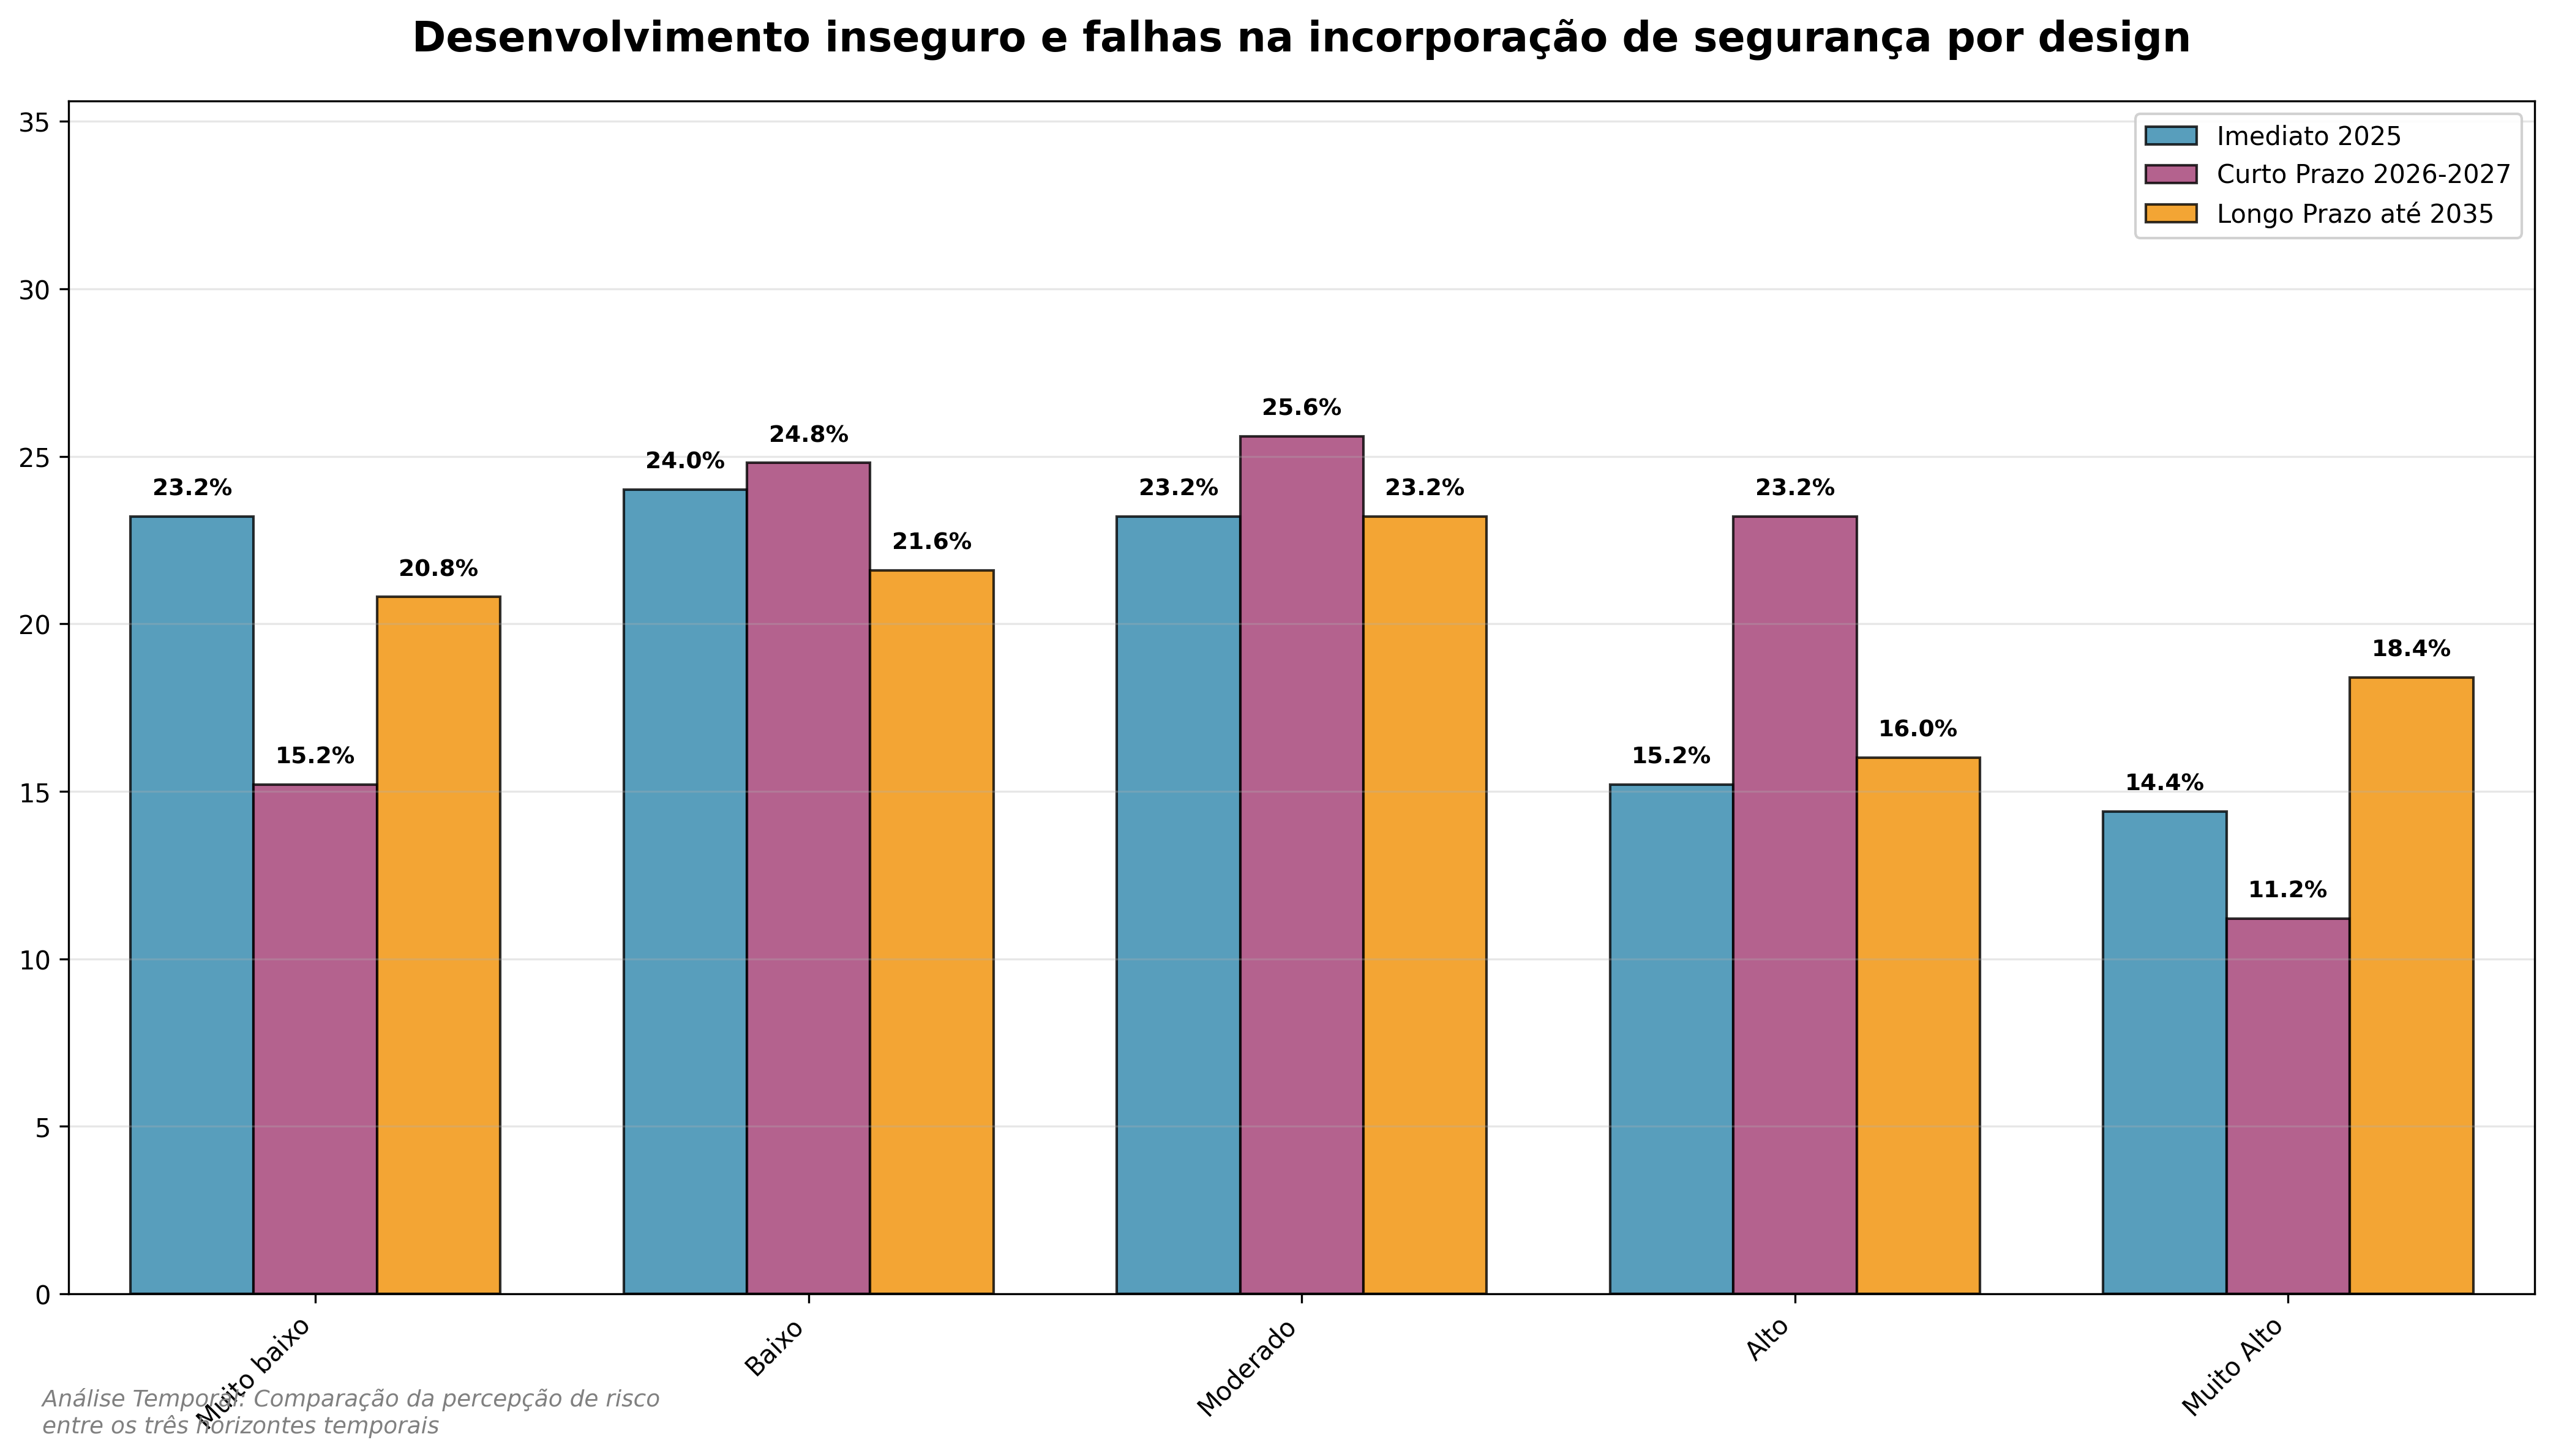
\includegraphics[keepaspectratio]{assets/tecnologicos/grafico_agrupado_5_14_temporal.png}}

\begin{tcolorbox}[enhanced jigsaw, titlerule=0mm, colback=white, title=\textcolor{quarto-callout-tip-color}{\faLightbulb}\hspace{0.5em}{Destaques}, opacityback=0, colbacktitle=quarto-callout-tip-color!10!white, leftrule=.75mm, left=2mm, colframe=quarto-callout-tip-color-frame, bottomrule=.15mm, bottomtitle=1mm, breakable, toprule=.15mm, toptitle=1mm, opacitybacktitle=0.6, arc=.35mm, coltitle=black, rightrule=.15mm]

\textbf{Imediato (2025)}: Mediana 3.0, 30\% em risco alto

\textbf{Curto Prazo (2026-2027)}: Mediana 3.0, 34\% em risco alto

\textbf{Longo Prazo (até 2035)}: Mediana 3.0, 34\% em risco alto

\textbf{Análise - Desenvolvimento inseguro e falhas na incorporação de
segurança por design} \textbf{Imediato (2025)}: Devido ao
desenvolvimento insuficiente de práticas de segurança por design e
falhas na incorporação de controles robustos, poderá acontecer a
implementação de sistemas digitais e automatizados com vulnerabilidades
exploráveis, o que poderá levar a incidentes cibernéticos localizados,
interrupções operacionais pontuais e exposição parcial de dados
sensíveis, impactando na confiabilidade das soluções tecnológicas e na
resiliência do ecossistema logístico dos portos brasileiros.

\textbf{Curto prazo (2026-2027)}: Devido a práticas ainda incipientes na
incorporação consistente de segurança por design durante o
desenvolvimento de sistemas digitais e automatizados no setor portuário
brasileiro, poderá acontecer a existência de vulnerabilidades moderadas
em soluções tecnológicas, o que poderá levar a tentativas eventuais de
ataques cibernéticos e interrupções pontuais nas operações, impactando
na confiabilidade dos sistemas e exigindo aprimoramento contínuo na
gestão da segurança da informação.

\textbf{Longo prazo (até 2035)}: Devido a práticas de desenvolvimento
que ainda não incorporam plenamente os princípios de segurança por
design, poderá acontecer a implementação de sistemas digitais e
automatizados com vulnerabilidades exploráveis, o que poderá levar a
incidentes cibernéticos pontuais, interrupções temporárias nas operações
portuárias e exposição parcial de dados sensíveis, impactando na
confiabilidade das soluções tecnológicas e na resiliência do ecossistema
logístico brasileiro no longo prazo.

\end{tcolorbox}

\subsection{Custo de implementação de novas
tecnologias}\label{custo-de-implementauxe7uxe3o-de-novas-tecnologias}

O gr?fico a seguir apresenta a evolu??o temporal do risco Custo de
implementação de novas tecnologias.
\pandocbounded{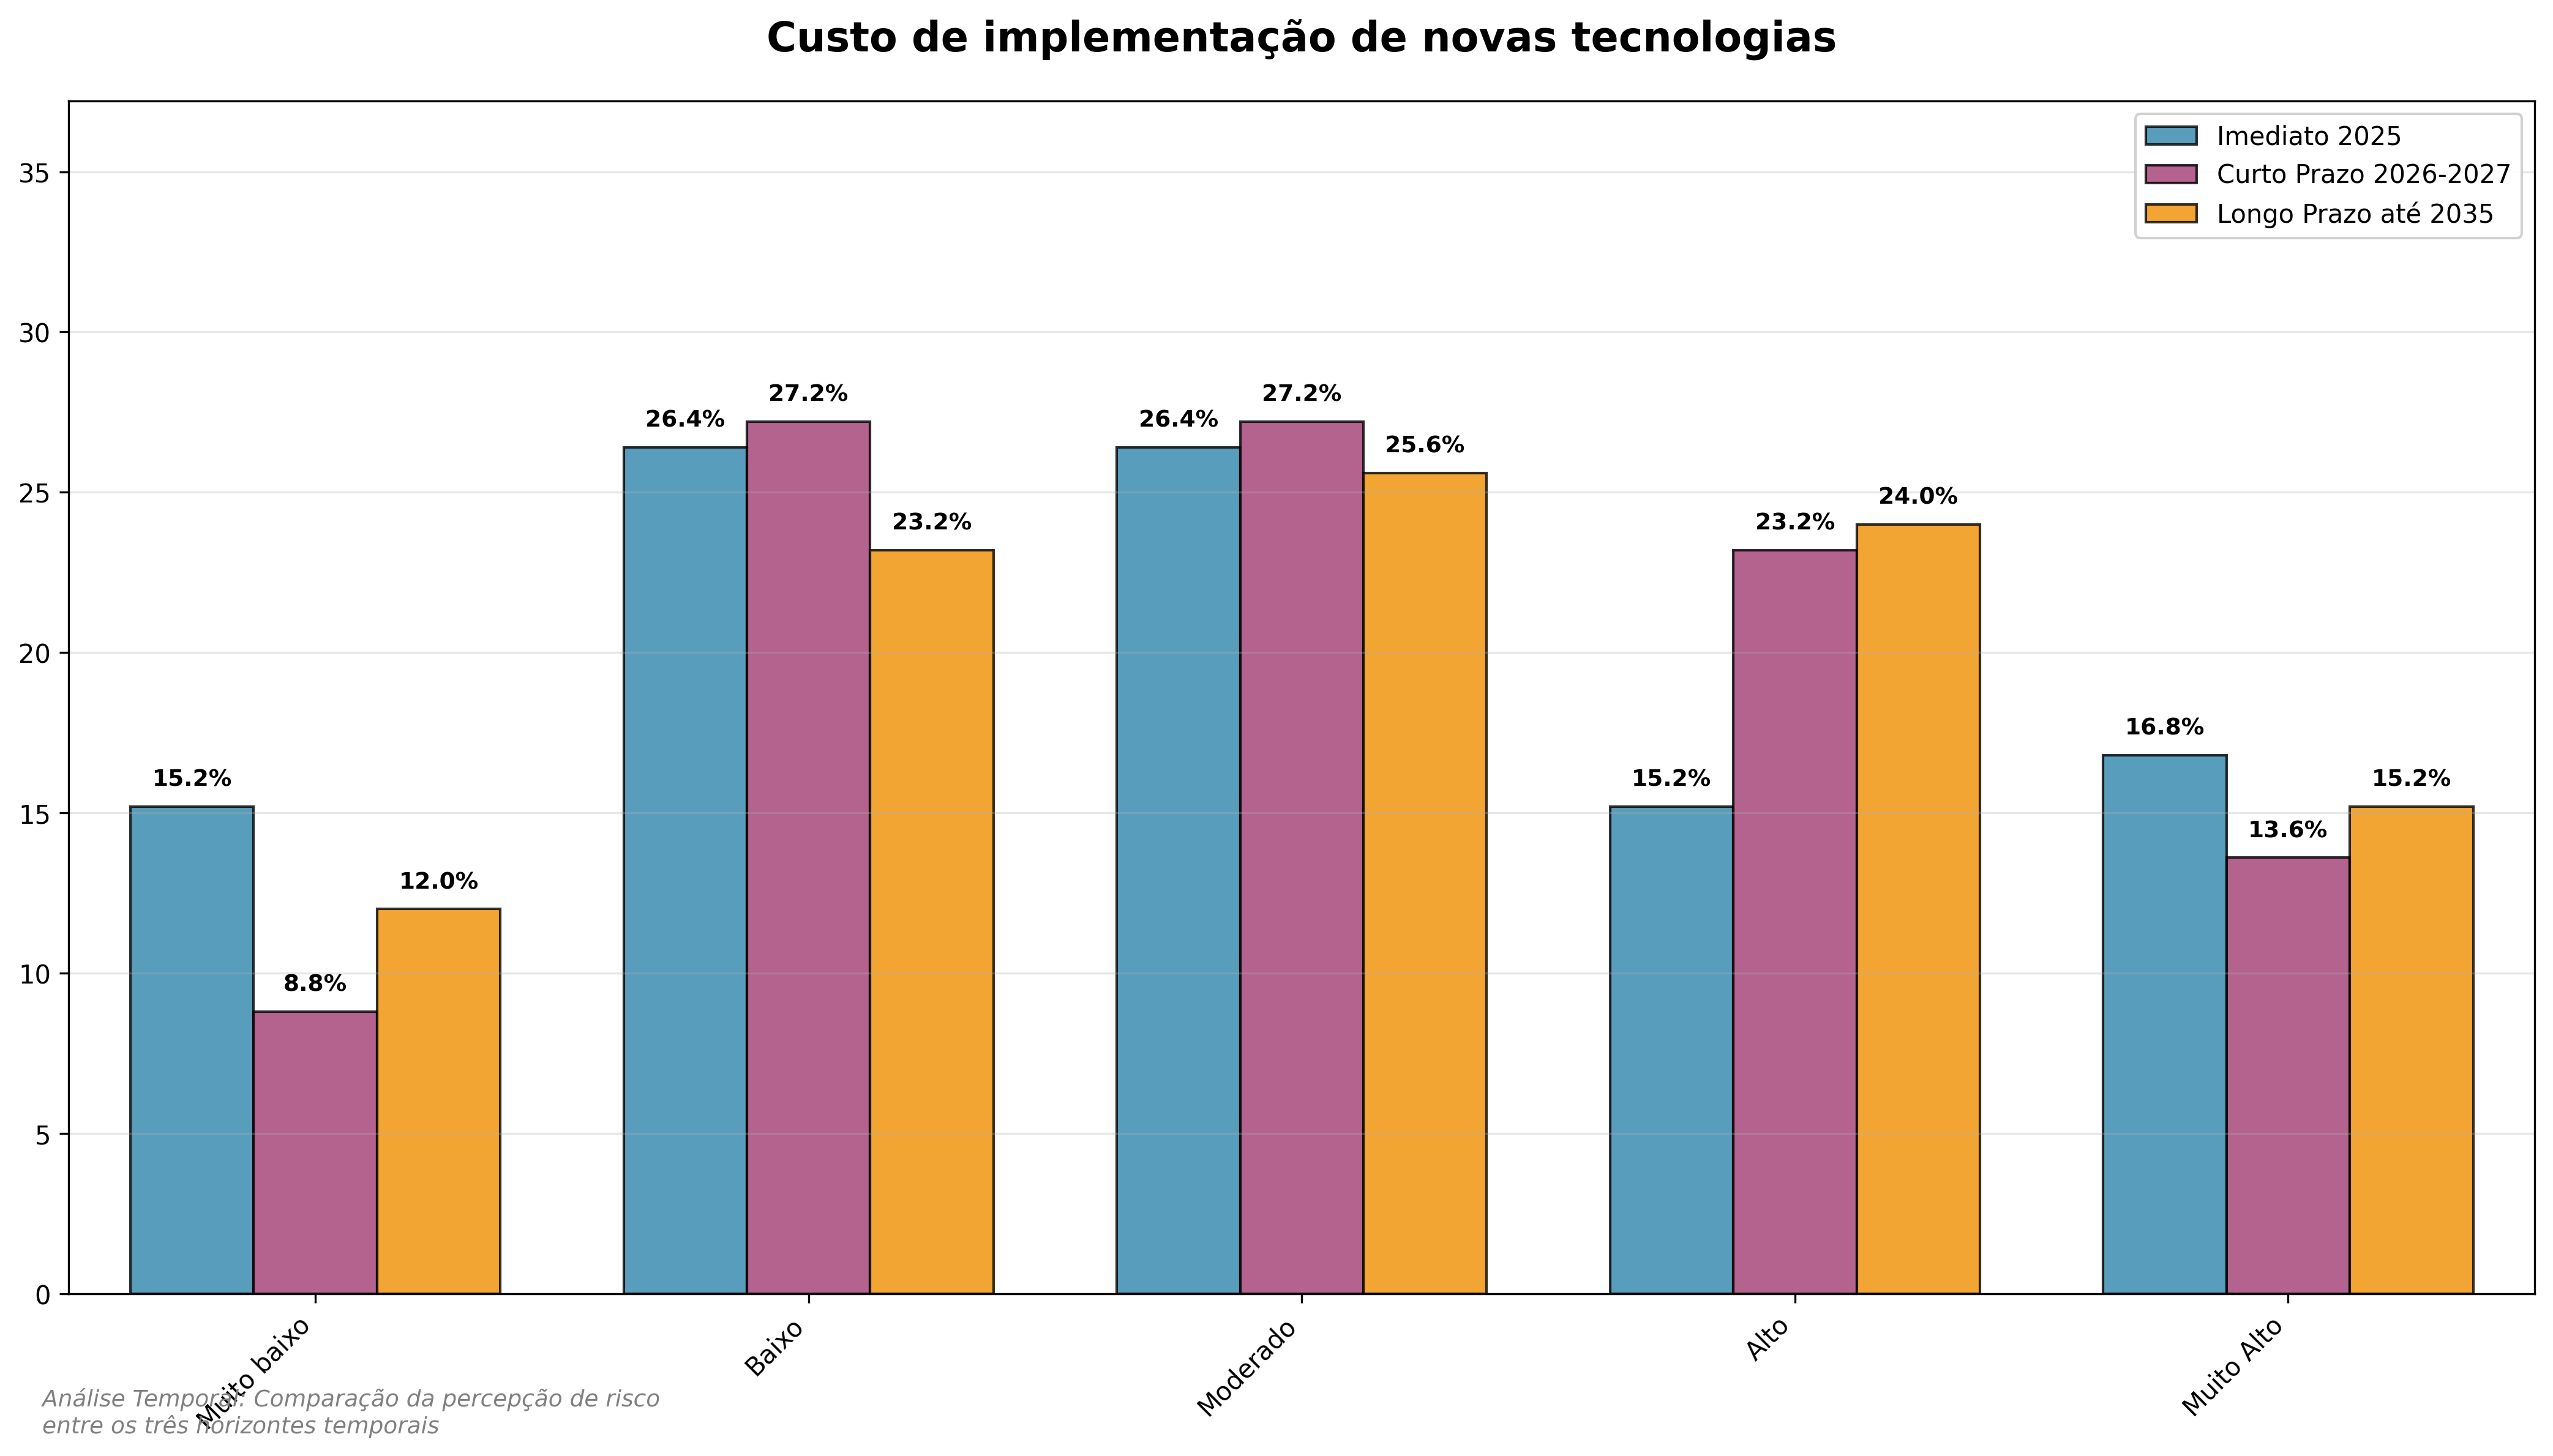
\includegraphics[keepaspectratio]{assets/tecnologicos/grafico_agrupado_5_15_temporal.png}}

\begin{tcolorbox}[enhanced jigsaw, titlerule=0mm, colback=white, title=\textcolor{quarto-callout-tip-color}{\faLightbulb}\hspace{0.5em}{Destaques}, opacityback=0, colbacktitle=quarto-callout-tip-color!10!white, leftrule=.75mm, left=2mm, colframe=quarto-callout-tip-color-frame, bottomrule=.15mm, bottomtitle=1mm, breakable, toprule=.15mm, toptitle=1mm, opacitybacktitle=0.6, arc=.35mm, coltitle=black, rightrule=.15mm]

\textbf{Imediato (2025)}: Mediana 3.0, 32\% em risco alto

\textbf{Curto Prazo (2026-2027)}: Mediana 3.0, 37\% em risco alto

\textbf{Longo Prazo (até 2035)}: Mediana 3.0, 39\% em risco alto

\textbf{Análise - Custo de implementação de novas tecnologias}
\textbf{Imediato (2025)}: Devido ao custo moderado de implementação de
novas tecnologias, poderá acontecer que alguns portos e terminais
enfrentem limitações financeiras para investir em modernização, o que
poderá levar ao adiamento parcial de projetos tecnológicos, impactando
de forma moderada a competitividade e eficiência do setor portuário
brasileiro no curto prazo.

\textbf{Curto prazo (2026-2027)}: Devido ao custo moderado de
implementação de novas tecnologias, poderá acontecer que alguns
investimentos necessários exijam maior esforço financeiro por parte dos
portos e terminais brasileiros, o que poderá levar ao adiamento pontual
de projetos de modernização, impactando na eficiência operacional e
competitividade do setor portuário no curto prazo.

\textbf{Longo prazo (até 2035)}: Devido ao custo crescente e à
complexidade na implementação de novas tecnologias, poderá acontecer que
os investimentos necessários desafiem a capacidade financeira dos portos
e terminais brasileiros, o que poderá levar a atrasos ou revisões nos
planejamentos dos projetos de modernização, impactando moderadamente na
competitividade e eficiência do setor portuário no longo prazo.

\end{tcolorbox}

\subsection{Escassez de mão de obra qualificada na área de
tecnologia}\label{escassez-de-muxe3o-de-obra-qualificada-na-uxe1rea-de-tecnologia}

O gr?fico a seguir apresenta a evolu??o temporal do risco Escassez de
mão de obra qualificada na área de tecnologia.
\pandocbounded{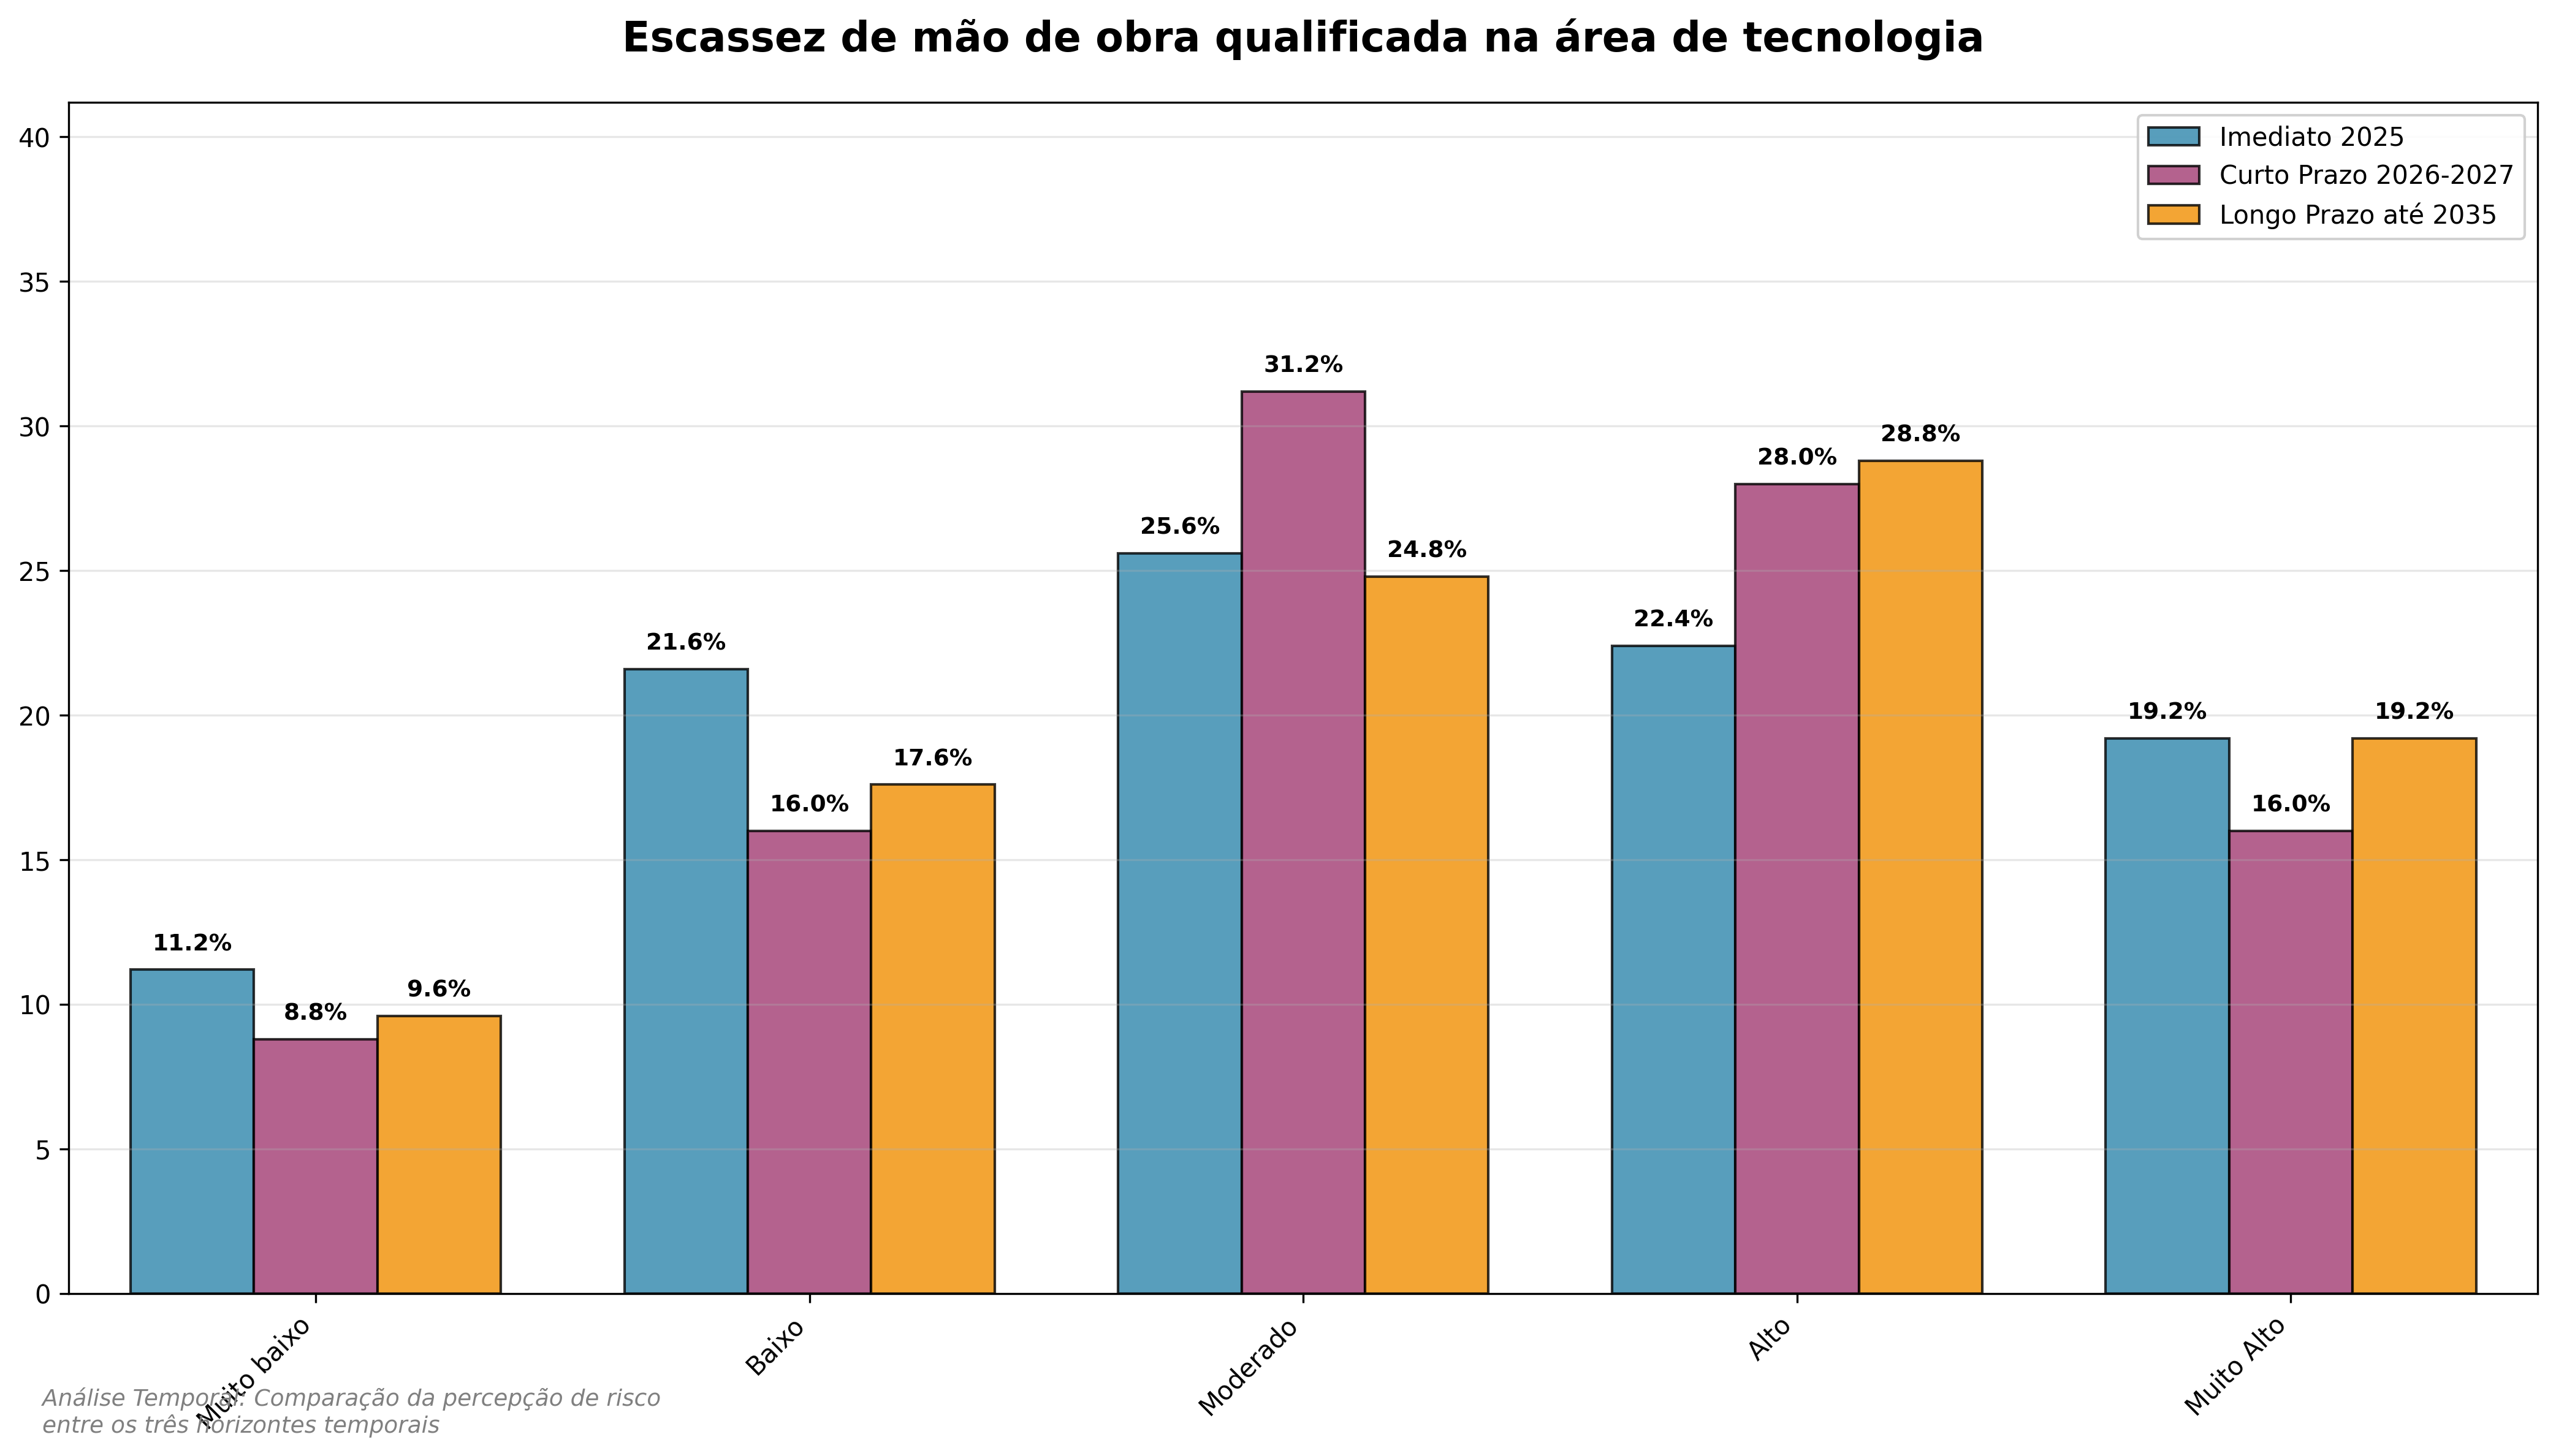
\includegraphics[keepaspectratio]{assets/tecnologicos/grafico_agrupado_5_16_temporal.png}}

\begin{tcolorbox}[enhanced jigsaw, titlerule=0mm, colback=white, title=\textcolor{quarto-callout-tip-color}{\faLightbulb}\hspace{0.5em}{Destaques}, opacityback=0, colbacktitle=quarto-callout-tip-color!10!white, leftrule=.75mm, left=2mm, colframe=quarto-callout-tip-color-frame, bottomrule=.15mm, bottomtitle=1mm, breakable, toprule=.15mm, toptitle=1mm, opacitybacktitle=0.6, arc=.35mm, coltitle=black, rightrule=.15mm]

\textbf{Imediato (2025)}: Mediana 3.0, 42\% em risco alto

\textbf{Curto Prazo (2026-2027)}: Mediana 3.0, 44\% em risco alto

\textbf{Longo Prazo (até 2035)}: Mediana 3.0, 48\% em risco alto

\textbf{Análise - Escassez de mão de obra qualificada na área de
tecnologia} \textbf{Imediato (2025)}: Devido à disponibilidade limitada
de mão de obra qualificada na área de tecnologia, poderá acontecer
dificuldade moderada na atração, capacitação e retenção de profissionais
especializados, o que poderá levar a atrasos pontuais na implementação
de projetos estratégicos, aumento controlado dos custos operacionais e
redução parcial da eficiência, impactando na capacidade dos portos
brasileiros de responder com agilidade adequada a incidentes e inovações
tecnológicas do mercado.

\textbf{Curto prazo (2026-2027)}: Devido à persistente escassez moderada
de mão de obra qualificada na área de tecnologia, poderá acontecer
dificuldades pontuais na atração, capacitação e retenção de
profissionais especializados nos portos brasileiros, o que poderá levar
a atrasos parciais na execução de projetos tecnológicos, elevação
moderada dos custos operacionais e alguma redução na eficiência dos
processos, impactando na capacidade do setor portuário de responder com
agilidade a incidentes e às demandas por inovação tecnológica no curto
prazo.

\textbf{Longo prazo (até 2035)}: Devido a desafios persistentes na
formação e retenção de mão de obra qualificada em tecnologia, poderá
acontecer dificuldade moderada na atração e desenvolvimento de
profissionais especializados, o que poderá levar a atrasos pontuais na
implementação de projetos tecnológicos, elevação controlada dos custos
operacionais e redução parcial da eficiência, impactando na capacidade
dos portos brasileiros de responder com agilidade a incidentes e
adaptações às inovações do mercado ao longo do período até 2035.

\end{tcolorbox}

\section{Análise Temporal
Comparativa}\label{anuxe1lise-temporal-comparativa-4}

A análise comparativa da percepção dos riscos ao longo dos três
horizontes temporais (Imediato, Curto Prazo e Longo Prazo) revela uma
evolução clara na natureza das preocupações do setor portuário,
permitindo a identificação de tendências e a formulação de insights
estratégicos direcionados.

\subsection{Tendências
Identificadas}\label{tenduxeancias-identificadas-4}

A percepção de risco evolui de ameaças operacionais e imediatas para
vulnerabilidades estruturais e estratégicas ao longo do tempo.

\begin{itemize}
\item
  No horizonte imediato (2025), a principal preocupação se concentra nos
  riscos mais visíveis e de impacto direto, como a falta de segurança
  computacional e as vulnerabilidades em sistemas de IoT. Isso reflete
  um foco na defesa contra ameaças cibernéticas, como ataques de
  ransomware e interrupções de serviço, que representam o perigo mais
  tangível e imediato para a continuidade das operações.
\item
  No curto prazo (2026-2027), a atenção se desloca para as dores do
  crescimento da digitalização. Riscos como os desafios de
  interoperabilidade e as falhas em sistemas de automação ganham
  destaque. Isso indica que, após a fase inicial de adoção de
  tecnologias, os problemas de integração entre sistemas legados e
  novos, bem como a complexidade de gerenciar ambientes automatizados,
  tornam-se as principais fontes de preocupação.
\item
  No longo prazo (até 2035), a perspectiva se torna eminentemente
  estratégica. A escassez de mão de obra qualificada e a concentração de
  direitos sobre tecnologias (dependência de fornecedores) emergem como
  os riscos mais críticos. Isso demonstra uma compreensão madura de que,
  no futuro, a maior ameaça não será um ataque específico, mas sim a
  falta de capacidade interna (capital humano) e de autonomia (soberania
  tecnológica) para inovar e se defender de forma sustentável.
\end{itemize}

\subsection{Insights Estratégicos}\label{insights-estratuxe9gicos-1}

A evolução das tendências de risco exige uma resposta estratégica,
dinâmica e multifacetada, que vá além da simples mitigação de ameaças
imediatas:

\begin{enumerate}
\def\labelenumi{\arabic{enumi}.}
\tightlist
\item
  Segurança Digital como Alicerce: A preocupação persistente com a
  segurança cibernética em todos os horizontes reforça a necessidade de
  tratar o investimento em segurança não como um custo, mas como um
  pilar fundamental e contínuo para a operação. A segurança digital
  robusta é a base sobre a qual toda a transformação tecnológica deve
  ser construída.
\item
  Modernização Tecnológica Planejada: O destaque para os riscos de
  interoperabilidade e automação no curto prazo evidencia que a
  modernização não pode ser um processo desordenado. É crucial planejar
  a atualização sistemática de sistemas legados e adotar padrões que
  garantam a integração segura e eficiente, evitando a criação de um
  ambiente tecnológico fragmentado e vulnerável.
\item
  Capacitação Humana como Prioridade Estratégica: A ascensão da escassez
  de mão de obra como o risco mais crítico no longo prazo é um alerta
  claro. O investimento em treinamento, desenvolvimento e atração de
  talentos em tecnologia e cibersegurança não é mais uma questão de RH,
  mas uma prioridade estratégica para a sobrevivência e competitividade
  do setor.
\item
  Busca pela Autonomia Tecnológica: A crescente preocupação com a
  dependência de fornecedores sinaliza a necessidade de uma estratégia
  nacional para reduzir a vulnerabilidade a riscos geopolíticos e de
  aprisionamento tecnológico (vendor lock-in). Fomentar um ecossistema
  de inovação local e diversificar as fontes de tecnologia são ações
  cruciais para garantir a soberania e a resiliência do setor portuário
  brasileiro no longo prazo.
\end{enumerate}

\bookmarksetup{startatroot}

\chapter{Conclusões e
Recomendações}\label{conclusuxf5es-e-recomendauxe7uxf5es}

A presente análise de riscos portuários, baseada em pesquisa com 125
gestores do setor brasileiro, revela um cenário complexo e dinâmico que
exige ações coordenadas e imediatas. Os achados demonstram a
interconexão crítica entre diferentes dimensões de risco, com
implicações diretas para a competitividade e sustentabilidade do setor
portuário nacional.

\section{Síntese dos Achados}\label{suxedntese-dos-achados}

\begin{itemize}
\item
  \textbf{Seis riscos imediatos críticos} foram identificados com
  percepção acima de 40\% em níveis altos (4-5), concentrados em
  instabilidade política (50,4\%), excesso regulatório (46,4\%), aumento
  de impostos (45,6\%), conflitos geoeconômicos (46,4\%), disrupções em
  infraestruturas críticas digitais (44,8\%) e falhas em cadeias de
  suprimentos (40,0\%).
\item
  \textbf{Cronicidade elevada dos riscos}: 73,7\% das variáveis
  analisadas permanecem crônicas em curto e longo prazo, indicando que a
  maioria dos desafios identificados não é transitória, mas sim
  estrutural e persistente.
\item
  \textbf{Divergência temporal preocupante}: A dimensão ambiental
  apresenta a maior piora temporal (+0,56), enquanto a tecnológica
  mantém estabilidade (delta 0,00), expondo uma lacuna crítica entre
  pressão climática crescente e maturidade digital insuficiente.
\item
  \textbf{Concentração econômica de riscos}: Treze dos vinte maiores
  riscos imediatos pertencem à dimensão econômica, com média de 39\% das
  respostas em níveis altos, configurando um cenário de vulnerabilidade
  sistêmica.
\end{itemize}

\section{Recomendações
Prioritárias}\label{recomendauxe7uxf5es-priorituxe1rias}

\subsection{1. Coordenação Econômico-Geopolítica (Curto Prazo -
2025)}\label{coordenauxe7uxe3o-econuxf4mico-geopoluxedtica-curto-prazo---2025}

Criar célula integrada para monitoramento conjunto de instabilidade
política, conflitos geoeconômicos e impactos regulatórios sobre cadeias
essenciais. Esta iniciativa deve incluir:

\begin{itemize}
\tightlist
\item
  Centro de monitoramento conjunto entre autoridades portuárias, ANTAQ e
  representantes do setor privado;- Inventário completo de ativos
  críticos e vulnerabilidades associadas;- Desenvolvimento de playbooks
  de resposta rápida para cenários de crise;- Mecanismos de diálogo
  permanente com órgãos reguladores e legislativos. \#\#\# 2. Plano de
  Adaptação Climática Portuária (Médio Prazo - 2026-2027)
\end{itemize}

Priorizar obras resilientes e protocolos para eventos extremos nas áreas
com maior delta ambiental, com foco em:

\begin{itemize}
\tightlist
\item
  Infraestrutura de proteção contra aumento do nível do mar e eventos
  climáticos extremos;- Sistemas de gestão de resíduos perigosos e
  controle de agentes patogênicos;- Planos de evacuação e contingência
  para comunidades portuárias;- Formação de equipes multidisciplinares
  para resposta a incidentes ambientais. \#\#\# 3. Resiliência Digital e
  Capital Humano (Longo Prazo - até 2035)
\end{itemize}

Acelerar redundâncias tecnológicas e programas de qualificação,
contemplando:

\begin{itemize}
\item
  Plataforma de dados compartilhada entre todos os atores portuários;-
  Investimentos em sistemas de backup e recuperação de desastres
  digitais;- Programas massivos de capacitação tecnológica para força de
  trabalho;- Revisão regulatória baseada em risco e fundos de adaptação
  climática. \#\# Ações recomendadas
\item
  \textbf{Implementar sistema de monitoramento contínuo} dos indicadores
  de risco identificados, com atualização trimestral e dashboards
  acessíveis a todos os stakeholders relevantes.
\item
  \textbf{Desenvolver estudos complementares} aprofundando a análise de
  interconexão entre riscos, especialmente os efeitos cascata entre
  choques econômicos, pressões ambientais e vulnerabilidades
  tecnológicas.
\item
  \textbf{Estabelecer parcerias estratégicas} com instituições de
  pesquisa e desenvolvimento para inovação em soluções de adaptação
  climática e resiliência operacional.
\item
  \textbf{Criar fundo de adaptação portuária} com contribuições do setor
  público e privado para financiar as transformações necessárias,
  especialmente em infraestrutura resiliente e capacitação humana.
\item
  \textbf{Integrar análise de riscos ao planejamento estratégico} de
  cada autoridade portuária, garantindo que as decisões de investimento
  e expansão considerem sistematicamente as vulnerabilidades
  identificadas.
\end{itemize}

A análise revela que os portos brasileiros enfrentam uma encruzilhada
crítica: a necessidade de modernização e expansão convive com riscos
crescentes e interconectados. O sucesso na navegação deste cenário
dependerá da capacidade de coordenar ações entre diferentes dimensões,
antecipar mudanças e construir resiliência sistêmica. As recomendações
apresentadas oferecem um roteiro prático para transformar os desafios
identificados em oportunidades de fortalecimento do setor portuário
nacional.

\bookmarksetup{startatroot}

\chapter{Referências}\label{referuxeancias}

APLICAÇÃO de um dispositivo não tripulado para monitoramento de poluição
de água e sedimento no Porto de Gdynia. \textbf{Water}, {[}s.l.{]}, v.
15, n.~4, 2023.

ARGYRIOU, I.; TSOUTSOS, T. Assessing critical entities: risk management
for IoT devices in ports. \textbf{Journal of Marine Science and
Engineering}, {[}s.l.{]}, v. 12, n.~9, art. 1593, 2024. DOI:
https://doi.org/10.3390/jmse12091593.

ASARIOTIS, R. et al.~Climate change and seaports: hazards, impacts, and
policies and legislation for adaptation. \textbf{Anthropocene Coasts},
{[}s.l.{]}, v. 7, n.~1, art. 14, 2024. DOI:
https://doi.org/10.1007/s44218-024-00047-9.

CHANG, W. et al.~Resilience of regional container port network: based on
projection correlation and dynamic spatial Markov chain.
\textbf{Maritime Policy \& Management}, {[}s.l.{]}, v. 51, n.~2,
p.~207-226, 2024.

DEMIREL, H. et al.~A comprehensive risk assessment framework for mooring
risks at hydrocarbon berths using fuzzy rule-based Bayesian network and
multi-attribute decision-making. \textbf{Stochastic Environmental
Research and Risk Assessment}, {[}s.l.{]}, v. 38, n.~11, p.~4393-4414,
2024. DOI: https://doi.org/10.1007/s00477-024-02809-w.

ELMAKIS, O. et al.~OS-BREEZE: oil spills boundary red emission zone
estimation using unmanned surface vehicles. \textbf{Sensors},
{[}s.l.{]}, v. 24, n.~2, art. 703, 2024. DOI:
https://doi.org/10.3390/s24020703.

HOU, L. et al.~Reshaping port-city relationships through underground
logistics system: a mixed qualitative approach. \textbf{Cities},
{[}s.l.{]}, v. 154, art. 105395, 2024. DOI:
https://doi.org/10.1016/j.cities.2024.105395.

KHAN, R. U. et al.~Seaport hazardous cargo loading and unloading risk
assessment using interval type-2 fuzzy sets and Bayesian networks.
\textbf{ASCE-ASME Journal of Risk and Uncertainty in Engineering
Systems, Part A: Civil Engineering}, {[}s.l.{]}, v. 10, n.~1, 2024.

ROAD accident risk analysis of at- and near-port areas reflecting
regional heterogeneous characteristics. \textbf{Maritime Policy \&
Management}, {[}s.l.{]}, v. 52, n.~4, p.~627-641, 2025.

RODRIGUES, T. A. et al.~Assessing risk dimensions in dry port projects:
prioritization, interdependence and heterogeneity. \textbf{Maritime
Business Review}, {[}s.l.{]}, v. 9, n.~4, p.~311-330, 2024. DOI:
https://doi.org/10.1108/MABR-09-2023-0064.

ROZIRWAN et al.~Ecological risk assessment of heavy metal (Pb, Cu)
contamination in water, sediment, and polychaeta (\emph{Neoleanira
tetragona}) from coastal areas affected by aquaculture, urban rivers,
and ports in South Sumatra. \textbf{Journal of Ecological Engineering},
{[}s.l.{]}, v. 25, n.~1, p.~303-319, 2024.

SPATIAL analysis and risk evaluation for port crisis management using
integrated soft computing and GIS-based models: a case study of Jazan
Port, Saudi Arabia. \textbf{Sustainability}, {[}s.l.{]}, v. 16, n.~12,
art. 5131, 2024.

SYSTEMIC risk capability assessment methodology: a new approach for
evaluating inter-connected risks in seaport ecosystems. \textbf{Progress
in Disaster Science}, {[}s.l.{]}, v. 16, 2023.

ZHOU, W.; XUE, J. et al.~Composition and distribution of bacteria,
pathogens, and antibiotic resistance genes at Shanghai Port, China.
\textbf{Water}, {[}s.l.{]}, v. 16, n.~18, 2024.

\bookmarksetup{startatroot}

\chapter{Conceitos e Glossário}\label{conceitos-e-glossuxe1rio}

Este glossário apresenta definições dos principais termos e conceitos
utilizados na \textbf{Análise de Riscos Portuários}, facilitando a
compreensão dos conteúdos apresentados.

\section{DIMENSÃO ECONÔMICA}\label{dimensuxe3o-econuxf4mica}

\begin{longtable}[]{@{}
  >{\raggedright\arraybackslash}p{(\linewidth - 4\tabcolsep) * \real{0.3333}}
  >{\raggedright\arraybackslash}p{(\linewidth - 4\tabcolsep) * \real{0.3333}}
  >{\raggedright\arraybackslash}p{(\linewidth - 4\tabcolsep) * \real{0.3333}}@{}}
\toprule\noalign{}
\begin{minipage}[b]{\linewidth}\raggedright
N°
\end{minipage} & \begin{minipage}[b]{\linewidth}\raggedright
RISCO
\end{minipage} & \begin{minipage}[b]{\linewidth}\raggedright
DEFINIÇÃO
\end{minipage} \\
\midrule\noalign{}
\endhead
\bottomrule\noalign{}
\endlastfoot
1 & Especulação e crise no mercado de ativos financeiros & Refere-se ao
aumento do passivo financeiro do Estado, decorrente de políticas fiscais
deficitárias ou crescimento das despesas públicas. O excesso de
endividamento reduz a capacidade governamental de investir em obras de
infraestrutura e eleva a vulnerabilidade macroeconômica do país. \\
2 & Concentração de recursos e controle de preços por agentes econômicos
& Concentração de recursos estrategicamente importantes (minerais,
materiais, tecnologias) entre um pequeno número de indivíduos, empresas
ou Estados que podem controlar o acesso e ditar preços
discricionários. \\
3 & Elevado endividamento público & Refere-se ao aumento do passivo
financeiro do Estado, decorrente de políticas fiscais deficitárias ou
crescimento das despesas públicas. O excesso de endividamento reduz a
capacidade governamental de investir em obras de infraestrutura e eleva
a vulnerabilidade macroeconômica do país. \\
4 & Elevado endividamento empresarial & Refere-se ao crescimento das
dívidas corporativas de empresas privadas, especialmente do setor de
transporte, logística e exportação, o que compromete a solvência, reduz
a competitividade e limita a capacidade de investimento em inovação e
sustentabilidade. \\
5 & Elevado endividamento das pessoas & Refere-se ao aumento do
comprometimento da renda das famílias com dívidas de consumo e crédito,
o que reduz o poder de compra, desacelera o mercado interno e afeta
indiretamente a demanda por bens e serviços movimentados pelos
portos. \\
6 & Falhas, interrupções ou disrupções em cadeias de suprimentos &
Refere-se a eventos que rompem ou atrasam fluxos logísticos essenciais,
como transporte marítimo, rodoviário ou ferroviário, provocando
desabastecimento, aumento de custos e impacto direto sobre a
produtividade e o comércio exterior. \\
7 & Disrupções em infraestruturas críticas (físicas e digitais) ou
serviços que sustentam sistemas críticos & Disrupções em infraestruturas
críticas (físicas e digitais) ou serviços que sustentam sistemas
críticos (internet, telecomunicações, serviços públicos, sistemas
financeiros ou energia). \\
8 & Estagnação do ritmo e da dinâmica das atividades econômicas &
Refere-se à desaceleração generalizada da economia, caracterizada por
baixo crescimento do PIB, retração do investimento e queda da produção
industrial, fatores que reduzem o volume de cargas e a receita
portuária. \\
9 & Ação do crime organizado e atividades ilícitas de empresas e pessoas
& Refere-se à infiltração de grupos criminosos em cadeias logísticas,
com práticas de contrabando, corrupção, lavagem de dinheiro e tráfico.
Essas ações comprometem a integridade institucional, aumentam custos
operacionais e afetam a imagem internacional do país. \\
10 & Aumento da inflação & Refere-se ao crescimento generalizado e
sustentado dos preços de bens e serviços, que reduz o poder de compra,
eleva custos logísticos e desorganiza contratos de longo prazo do setor
portuário e industrial. \\
11 & Dificuldades de financiamento e investimento & Dificuldades de
financiamento e obtenção de recursos financeiros para investimento.
Refere-se à restrição de crédito e à elevação de juros que limitam o
acesso de empresas e governos a financiamentos para projetos de
infraestrutura, inovação e modernização portuária. \\
12 & Riscos reputacionais & Referem-se à possibilidade de danos à
reputação de uma organização devido a eventos, comportamentos, práticas
ou percepções negativas, que podem impactar a confiança e a
credibilidade da empresa perante stakeholders, incluindo clientes,
investidores, parceiros, funcionários e a sociedade em geral. \\
13 & Risco de competitividade portuária & Risco de competitividade
portuária. Riscos relacionados à concorrência entre portos referem-se às
ameaças e desafios que um porto enfrenta em seu desempenho operacional,
financeiro e estratégico devido à competição com outros portos que
oferecem serviços semelhantes ou atuam na mesma região geográfica ou
cadeia logística. \\
14 & Aumento de impostos & Elevação de tributos incidentes sobre
empresas e cidadãos, que reduz margens de lucro, encarece produtos e
compromete a competitividade dos portos e operadores logísticos. \\
15 & Instabilidade política & Ausência de consenso institucional,
mudanças abruptas de políticas públicas ou crises governamentais que
geram insegurança jurídica e desconfiança de investidores nacionais e
estrangeiros. \\
16 & Excesso regulatório & Sobreposição de normas, exigências e
processos burocráticos que aumentam custos de conformidade e reduzem a
eficiência administrativa e operacional do sistema portuário. \\
17 & Déficit regulatório & Ausência ou insuficiência de marcos
normativos claros e atualizados, o que gera insegurança jurídica,
lacunas de fiscalização e dificuldades de implementação de políticas
públicas. \\
18 & Aumento do desemprego & Redução do nível de ocupação formal e
informal, comprometendo a renda das famílias, a arrecadação tributária e
o consumo interno, com reflexos negativos na movimentação portuária. \\
19 & Aumento da corrupção & Prática de desvio de recursos, fraude em
contratos ou favorecimento indevido que compromete a transparência, a
eficiência administrativa e a credibilidade das instituições públicas e
privadas. \\
20 & Desequilíbrio econômico regional & Concentração desigual de
investimentos e oportunidades entre regiões do país, ampliando
disparidades produtivas e logísticas e dificultando o desenvolvimento de
corredores de exportação integrados. \\
21 & Conflito ou instabilidade institucional do Estado & Ruptura de
pactos políticos ou legais entre poderes e instituições, resultando em
insegurança jurídica, paralisia decisória e enfraquecimento da
governança nacional, com impactos diretos sobre o ambiente de negócios e
o investimento em infraestrutura. \\
\end{longtable}

\section{DIMENSÃO AMBIENTAL}\label{dimensuxe3o-ambiental}

\begin{longtable}[]{@{}
  >{\raggedright\arraybackslash}p{(\linewidth - 4\tabcolsep) * \real{0.3333}}
  >{\raggedright\arraybackslash}p{(\linewidth - 4\tabcolsep) * \real{0.3333}}
  >{\raggedright\arraybackslash}p{(\linewidth - 4\tabcolsep) * \real{0.3333}}@{}}
\toprule\noalign{}
\begin{minipage}[b]{\linewidth}\raggedright
N°
\end{minipage} & \begin{minipage}[b]{\linewidth}\raggedright
RISCO
\end{minipage} & \begin{minipage}[b]{\linewidth}\raggedright
DEFINIÇÃO
\end{minipage} \\
\midrule\noalign{}
\endhead
\bottomrule\noalign{}
\endlastfoot
1 & Perda de biodiversidade e colapso de ecossistemas & Refere-se à
redução da variedade biológica em ambientes marinhos e costeiros,
provocada por poluição, dragagens, desmatamento e ocupações irregulares.
A perda de espécies e habitats compromete serviços ecossistêmicos
essenciais, como proteção natural do litoral, regulação climática e
suporte à pesca, gerando desequilíbrios ambientais e socioeconômicos
duradouros. \\
2 & Eventos que possam impactar acessos e operações como deslizamentos,
desmoronamentos e assoreamentos & Eventos que possam impactar acessos e
operações portuárias, como deslizamentos ou desmoronamentos de encostas
e margens (terras caídas) e o assoreamento acelerado de rios e canais de
navegação. \\
3 & Mudanças climáticas & Mudanças climáticas (intensificação e aumento
da frequência de fenômenos como chuvas, tempestades, vendavais, ondas de
calor, secas, ciclones e furacões). \\
4 & Crise na disponibilidade de recursos naturais como água e produção
de alimentos & A escassez de água pode afetar diretamente o
abastecimento em portos e terminais, enquanto a redução na produção de
alimentos impacta a logística de exportação e importação, reduzindo
fluxos de carga e a competitividade portuária. \\
5 & Desastres naturais não relacionados à atuação do homem em mudanças
climáticas & Desastres naturais não relacionados ao clima, como
terremotos, incêndios florestais, maremotos, subsidência. \\
6 & Aumento do nível do mar e processos erosivos costeiros & Refere-se à
elevação gradual do nível médio do mar e à intensificação da erosão
litorânea, fenômenos agravados pelas mudanças climáticas. Esses
processos afetam diretamente áreas portuárias, cais, retroáreas e zonas
urbanas adjacentes, causando prejuízos estruturais, redução de áreas
operacionais e necessidade de investimentos em adaptação e engenharia
costeira. \\
7 & Poluição da água e sedimentos em áreas portuárias por contaminantes
& Poluição da água e sedimentos em áreas portuárias por contaminantes
orgânicos e inorgânicos, tais como hidrocarbonetos, metais, pesticidas e
nutrientes. \\
8 & Movimentação de produtos perigosos & Refere-se ao manuseio,
transporte e armazenamento de substâncias inflamáveis, tóxicas ou
poluentes nos portos. Falhas de contenção, vazamentos ou acidentes podem
gerar contaminação do solo e da água, riscos à saúde humana e danos
irreversíveis à fauna e flora marinha, exigindo protocolos rigorosos de
segurança e resposta a emergências. \\
9 & Presença de agentes patogênicos relacionados ao saneamento &
Presença de agentes patogênicos por deficiência no tratamento de esgoto
ou saneamento. \\
10 & Introdução de espécies exóticas & Espécies exóticas, organismos
aquáticos nocivos e agentes patogênicos introduzidos por operações
marítimas e portuárias. \\
11 & Poluição atmosférica & Emissão de gases e partículas provenientes
da queima de combustíveis fósseis em embarcações, caminhões e
equipamentos portuários. Esses poluentes contribuem para o aquecimento
global e agravam problemas respiratórios nas populações vizinhas,
demandando o uso de combustíveis limpos, tecnologias de exaustão e
monitoramento contínuo da qualidade do ar. \\
12 & Ruídos e vibrações & Emissão de sons e trepidações gerados por
operações de carga e descarga, dragagens e tráfego de veículos. Esses
impactos afetam comunidades próximas, ecossistemas aquáticos e espécies
sensíveis, podendo gerar conflitos socioambientais e exigindo controle
acústico e planejamento operacional adequado. \\
13 & Gerenciamento inadequado dos resíduos sólidos & Disposição
incorreta de resíduos portuários, industriais e domésticos, resultando
em poluição do solo, contaminação hídrica e proliferação de vetores. A
ausência de segregação, coleta seletiva e tratamento adequado compromete
o cumprimento da Política Nacional de Resíduos Sólidos e as metas
ambientais de portos sustentáveis. \\
14 & Aumento do desmatamento & Supressão de vegetação nativa em áreas de
expansão portuária e retroportuária, reduzindo a proteção natural contra
erosão e perda de biodiversidade. Essa prática intensifica a emissão de
gases de efeito estufa e dificulta a recuperação ambiental de áreas
sensíveis. \\
15 & Dificuldades na obtenção e manutenção do licenciamento ambiental &
Processo legal que autoriza a instalação e operação de empreendimentos
portuários mediante análise dos impactos ambientais. Atrasos,
inconsistências técnicas ou falta de cumprimento das condicionantes
podem gerar paralisações, sanções e perda de credibilidade
institucional. \\
16 & Descarbonização do transporte marítimo & Transição gradual do setor
marítimo e portuário para o uso de combustíveis e tecnologias de baixo
carbono, com o objetivo de reduzir emissões de gases de efeito estufa. A
adoção de navios elétricos, biocombustíveis e infraestrutura para
hidrogênio verde é estratégica, mas depende de investimentos e regulação
internacional coordenada. \\
17 & Reduzido nível de educação e conscientização ambiental & Limitado
engajamento de trabalhadores, gestores e comunidades na adoção de
práticas sustentáveis. A ausência de programas de capacitação e
sensibilização ambiental dificulta o cumprimento de metas de
sustentabilidade e o fortalecimento da cultura ambiental nas operações
portuárias. \\
\end{longtable}

\begin{center}\rule{0.5\linewidth}{0.5pt}\end{center}

\section{DIMENSÃO GEOPOLÍTICA}\label{dimensuxe3o-geopoluxedtica}

\begin{longtable}[]{@{}
  >{\raggedright\arraybackslash}p{(\linewidth - 4\tabcolsep) * \real{0.3333}}
  >{\raggedright\arraybackslash}p{(\linewidth - 4\tabcolsep) * \real{0.3333}}
  >{\raggedright\arraybackslash}p{(\linewidth - 4\tabcolsep) * \real{0.3333}}@{}}
\toprule\noalign{}
\begin{minipage}[b]{\linewidth}\raggedright
N°
\end{minipage} & \begin{minipage}[b]{\linewidth}\raggedright
RISCO
\end{minipage} & \begin{minipage}[b]{\linewidth}\raggedright
DEFINIÇÃO
\end{minipage} \\
\midrule\noalign{}
\endhead
\bottomrule\noalign{}
\endlastfoot
1 & Liberação intencional ou acidental de contaminante biológico,
químico, nuclear ou radiológico & Situação em que ocorre o despejo,
vazamento ou disseminação de substâncias perigosas, de forma acidental
ou deliberada, em ambientes portuários, marítimos ou urbanos adjacentes.
Esses contaminantes podem provocar danos graves à saúde humana, à fauna
e à flora, além de comprometer a qualidade da água, do ar e do solo.
Eventos desse tipo exigem protocolos rigorosos de prevenção, contenção e
resposta a emergências, integrando planos de segurança, defesa civil e
monitoramento ambiental para reduzir impactos imediatos e de longo
prazo. \\
2 & Alterações em condições de sistemas terrestres & Mudanças em
fronteiras territoriais, disputas por soberania em áreas estratégicas,
delimitações marítimas e controle de recursos naturais que impactam
rotas comerciais e cadeias logísticas globais. \\
3 & Conflitos geoeconômicos como bloqueios, sanções, restrições
tarifárias e redução de investimentos & Conflitos geoeconômicos
(bloqueios, sanções, restrições tarifárias, redução de investimentos)
correspondem a disputas econômicas entre países ou blocos comerciais que
utilizam instrumentos financeiros e comerciais como forma de pressão
política ou estratégica. Esses eventos podem provocar interrupções nas
cadeias de suprimentos, aumento de custos logísticos, escassez de
insumos e retração de investimentos estrangeiros. No contexto portuário,
tais conflitos afetam o volume de comércio exterior, a previsibilidade
das rotas marítimas e a estabilidade econômica de regiões dependentes da
exportação e importação de commodities. \\
4 & Conflitos armados entre nações & Conflitos armados entre nações
representam situações de confronto militar direto entre Estados, capazes
de interromper rotas marítimas, gerar bloqueios portuários e comprometer
a segurança de tripulações e cargas. Além dos impactos humanitários e
políticos, esses conflitos afetam o comércio internacional, elevam
custos de seguros, reduzem a disponibilidade de combustíveis e
desorganizam cadeias logísticas globais. O setor portuário torna-se
particularmente vulnerável a interrupções operacionais e à instabilidade
econômica resultante da guerra. \\
5 & Violência e crises internas em países parceiros como greves gerais,
conflitos internos, golpes de Estado e insegurança pública & Violência
aberta em países de relação, como greves, conflitos internos, golpes de
Estado e situações de insegurança pública, afeta diretamente o ambiente
político e econômico de nações com as quais o Brasil mantém vínculos
comerciais. Esses eventos reduzem a estabilidade institucional,
comprometem contratos internacionais e podem interromper cadeias
logísticas essenciais. No setor portuário, a instabilidade nos países
parceiros se traduz em atrasos de embarques, cancelamentos de rotas,
aumento de custos de transporte e riscos à integridade física de
trabalhadores e ativos estratégicos. \\
6 & Terrorismo & Prática de atos violentos com motivação política,
ideológica ou religiosa que visam causar medo, destruição e
instabilidade social. No contexto portuário, envolve ameaças a
infraestruturas críticas, terminais, embarcações e cadeias logísticas
internacionais. Atentados, sabotagens e uso de artefatos explosivos
podem provocar perdas humanas, danos materiais e paralisação de
operações estratégicas. A prevenção e a resposta ao terrorismo exigem
cooperação entre autoridades portuárias, forças de segurança e
organismos internacionais, com foco em inteligência, vigilância e
protocolos de emergência integrados. \\
7 & Migração ou deslocamento forçado & Migração ou deslocamento forçado
(involuntário), envolvendo força, compulsão ou coerção, devido a fatores
diversos (conflitos, desastres naturais, instabilidade política e
econômica, mudanças climáticas e perseguição identitária, religiosa,
étnica, cultural ou política). Fluxos migratórios massivos podem ser
utilizados como instrumento de pressão política entre Estados,
impactando negociações internacionais, políticas de fronteira e a
estabilidade de regiões estratégicas. \\
\end{longtable}

\begin{center}\rule{0.5\linewidth}{0.5pt}\end{center}

\section{DIMENSÃO SOCIAL}\label{dimensuxe3o-social-1}

\begin{longtable}[]{@{}
  >{\raggedright\arraybackslash}p{(\linewidth - 4\tabcolsep) * \real{0.3333}}
  >{\raggedright\arraybackslash}p{(\linewidth - 4\tabcolsep) * \real{0.3333}}
  >{\raggedright\arraybackslash}p{(\linewidth - 4\tabcolsep) * \real{0.3333}}@{}}
\toprule\noalign{}
\begin{minipage}[b]{\linewidth}\raggedright
N°
\end{minipage} & \begin{minipage}[b]{\linewidth}\raggedright
RISCO
\end{minipage} & \begin{minipage}[b]{\linewidth}\raggedright
DEFINIÇÃO
\end{minipage} \\
\midrule\noalign{}
\endhead
\bottomrule\noalign{}
\endlastfoot
1 & Ameaças aos direitos humanos e/ou às liberdades individuais ou de
grupo & Ameaças aos direitos humanos e às liberdades individuais ou de
grupo envolvem situações em que ações institucionais, empresariais ou
políticas restringem a dignidade, a igualdade de tratamento e a livre
expressão das pessoas ou comunidades afetadas pelas atividades
portuárias. Esses riscos podem manifestar-se por meio de práticas
discriminatórias, repressão de manifestações, limitações ao direito de
associação sindical ou violação do direito à moradia em áreas impactadas
por projetos de expansão portuária. Na relação porto-cidade, a
fragilidade na proteção de direitos humanos gera tensões sociais, perda
de legitimidade institucional e aumento da vulnerabilidade de grupos
marginalizados. A promoção e a defesa desses direitos exigem políticas
de governança inclusiva, mecanismos de transparência, canais de denúncia
acessíveis e o cumprimento de normas nacionais e internacionais que
garantam justiça social e respeito à cidadania. \\
2 & Ocorrência de pandemias ou epidemias & Ocorrência de pandemias ou
epidemias representa a disseminação de doenças contagiosas em escala
local, regional ou global, com potencial de afetar gravemente a saúde
pública, a economia e a logística portuária. No contexto porto-cidade, a
circulação internacional de pessoas e mercadorias amplia a exposição a
agentes infecciosos e exige protocolos rigorosos de vigilância
sanitária, controle de fronteiras e segurança ocupacional. Esses eventos
provocam redução de fluxos comerciais, interrupção de cadeias de
suprimentos, afastamento de trabalhadores e aumento de custos
operacionais. A experiência recente de crises sanitárias, como a
pandemia de COVID-19, evidenciou a necessidade de portos resilientes,
capazes de manter serviços essenciais, adotar medidas de biossegurança e
atuar em coordenação com autoridades de saúde e gestão pública para
mitigar impactos sociais e econômicos sobre as comunidades
portuárias. \\
3 & Insuficiência de serviços públicos essenciais que impactam a força
de trabalho & Insuficiência de serviços públicos essenciais, como saúde,
saneamento, transporte, segurança e educação, que impacta diretamente a
qualidade de vida da população e a força de trabalho vinculada ao setor
portuário. \\
4 & Impactos geopolíticos & Refere-se à vulnerabilidade dos portos a
eventos disruptivos, incluindo conflitos geopolíticos e disrupções
ambientais, que podem afetar a resiliência da rede portuária e
comprometer a continuidade das operações. \\
5 & Acidentes rodoviários e ferroviários de alta severidade em áreas
próximas aos portos & Acidentes rodoviários e ferroviários de alta
severidade em áreas próximas aos portos representam um dos principais
riscos operacionais e urbanos da relação porto-cidade. Esses eventos,
muitas vezes associados ao intenso fluxo de caminhões, trens e
maquinários pesados, podem causar perdas humanas, danos materiais
significativos e impactos ambientais relevantes. A proximidade entre
zonas residenciais e corredores logísticos aumenta o potencial de
colisões, vazamentos de cargas perigosas e congestionamentos críticos. A
ausência de planejamento urbano integrado, infraestrutura viária
adequada e sistemas inteligentes de tráfego agrava a frequência e a
gravidade dos acidentes. \\
6 & Acidentes nas operações portuárias & Acidentes nas operações
portuárias correspondem a eventos que ocorrem durante atividades de
carga, descarga, transporte interno, atracação e manutenção de
embarcações ou equipamentos, podendo resultar em ferimentos, perdas
materiais e danos ambientais. Esses incidentes estão frequentemente
associados a falhas humanas, deficiências de treinamento, uso inadequado
de equipamentos, ausência de sinalização, sobrecarga de trabalho ou
condições climáticas adversas, bem como manutenção inadequada de
máquinas e equipamentos. Além de comprometer a segurança dos
trabalhadores e a continuidade operacional, os acidentes afetam a
reputação institucional e podem gerar custos elevados de indenização e
paralisação. A prevenção exige cultura de segurança consolidada,
cumprimento rigoroso das normas de saúde e segurança do trabalho,
capacitação contínua de equipes e adoção de tecnologias de monitoramento
e automação que reduzam a exposição humana a situações de risco. \\
7 & Falhas na gestão de crises e na resposta a emergências & Falhas na
gestão de crises e na resposta a emergências ocorrem quando os sistemas
institucionais e operacionais não conseguem agir de forma coordenada,
rápida e eficaz diante de eventos críticos como acidentes, desastres
ambientais, incêndios, ataques cibernéticos ou eventos climáticos
extremos. A ausência de planos integrados, comunicação eficiente e
treinamento contínuo gera respostas fragmentadas, atrasos na contenção
de danos e aumento das consequências sociais, ambientais e econômicas.
No contexto porto-cidade, essas falhas ampliam a vulnerabilidade das
comunidades do entorno e comprometem a confiança nas autoridades
públicas e portuárias. A gestão eficaz de crises requer protocolos
atualizados, simulações regulares, integração entre órgãos de defesa
civil, segurança, saúde e meio ambiente, além de mecanismos de
transparência e comunicação que assegurem o fluxo adequado de
informações durante situações emergenciais. \\
8 & Falhas no controle interno: fraudes ou corrupção & Falhas no
controle interno, incluindo fraudes ou corrupção, correspondem a
situações em que mecanismos de fiscalização, auditoria e governança não
são capazes de prevenir, detectar ou responder adequadamente a práticas
ilícitas dentro das instituições portuárias. Essas irregularidades podem
envolver desvio de recursos, manipulação de contratos, favorecimento
indevido ou ocultação de informações relevantes. Além de gerar prejuízos
financeiros e comprometer a eficiência administrativa, tais falhas
corroem a credibilidade institucional, reduzem a confiança dos
investidores e enfraquecem a transparência na relação porto-cidade. O
enfrentamento desse risco exige fortalecimento dos sistemas de controle
interno, aplicação de políticas de integridade, auditorias
independentes, canais de denúncia seguros e uma cultura organizacional
orientada à ética, à responsabilidade e à prestação de contas. \\
9 & Instabilidade gerada por alterações no marco regulatório e excesso
de judicialização & Insegurança jurídica relacionada à legislação
trabalhista, à flexibilização ou ao aumento da rigidez normativa e ao
impacto de processos judiciais sobre as relações de trabalho nos portos.
Instabilidade gerada por alterações no marco regulatório e excesso de
judicialização ocorre quando mudanças frequentes em leis, normas ou
diretrizes do setor portuário criam incertezas jurídicas e dificultam o
planejamento de longo prazo. A ausência de estabilidade normativa
compromete a previsibilidade dos investimentos, eleva os custos de
conformidade e desestimula a participação do setor privado em projetos
de infraestrutura. O aumento da judicialização, com disputas recorrentes
entre entes públicos, operadores e investidores, paralisa processos
decisórios, atrasa obras e impacta a competitividade dos portos. \\
10 & Falta de recursos humanos capacitados e especializados no setor
portuário & Falta de recursos humanos capacitados e especializados no
setor portuário está associada à carência de profissionais com domínio
técnico e gerencial necessários para atender às demandas complexas das
operações portuárias modernas. Essa limitação se manifesta na
dificuldade de adaptação às novas tecnologias, nos baixos índices de
produtividade e na dependência de mão de obra não qualificada para
atividades que exigem conhecimento em logística, automação, gestão
ambiental, segurança e governança portuária. A ausência de formação
continuada e de programas estruturados de capacitação reduz a capacidade
de inovação, compromete a competitividade e enfraquece a resiliência
institucional dos portos diante de transformações como a digitalização,
a descarbonização e a adoção de práticas ESG. \\
11 & Assédio (moral e sexual) no ambiente de trabalho & Assédio moral e
sexual no ambiente de trabalho compreende comportamentos abusivos,
constrangedores ou discriminatórios que violam a dignidade e a
integridade física ou psicológica dos trabalhadores. No contexto
portuário, esse tipo de conduta pode manifestar-se por meio de
intimidações, insultos, perseguições, chantagens, avanços indesejados ou
uso de posição hierárquica para constranger subordinados. Além de causar
danos emocionais e comprometer a produtividade, o assédio prejudica o
clima organizacional, desestimula a permanência de profissionais
qualificados e afeta a reputação institucional. A prevenção e o
enfrentamento desse risco exigem políticas claras de conduta ética,
canais de denúncia seguros, campanhas educativas e o fortalecimento de
uma cultura organizacional baseada no respeito e na igualdade. \\
12 & Desigualdades raciais/étnicas e de gênero & Desigualdades raciais,
étnicas e de gênero expressam a persistência de assimetrias estruturais
no mercado de trabalho portuário, refletidas em diferenças de acesso a
cargos, remuneração, qualificação e participação em processos
decisórios. Essas desigualdades limitam o potencial de inovação e
comprometem o equilíbrio social dentro das organizações, perpetuando
estereótipos e exclusões históricas. A ausência de políticas
institucionais de diversidade e inclusão amplia essas lacunas e reduz a
competitividade do setor. A promoção da equidade requer ações
afirmativas, programas de capacitação e mecanismos de monitoramento que
assegurem representatividade, igualdade de oportunidades e um ambiente
de trabalho pautado pela justiça social e pelo respeito à
diversidade. \\
13 & Falta de participação social & Falta de participação social na
relação porto-cidade ocorre quando comunidades locais, trabalhadores e
instituições da sociedade civil não são incluídos de forma efetiva nos
processos de planejamento, gestão e tomada de decisão sobre as
atividades portuárias e seus impactos urbanos. Essa ausência de diálogo
reduz a transparência, fragiliza a legitimidade das ações da autoridade
portuária e intensifica conflitos territoriais, ambientais e sociais nas
áreas de interface entre o porto e a cidade. A carência de mecanismos de
participação compromete a construção de soluções compartilhadas para
temas como mobilidade, uso do solo, habitação, qualidade ambiental e
geração de emprego. O fortalecimento da governança porto-cidade requer
instrumentos participativos permanentes, como conselhos comunitários,
audiências públicas e plataformas de diálogo, que promovam
corresponsabilidade e integração entre desenvolvimento econômico,
sustentabilidade e bem-estar das populações do entorno portuário. \\
14 & Maior uso de tecnologias (IA, mecanização, robotização) & Maior uso
de tecnologias como inteligência artificial, mecanização e robotização
transforma profundamente as operações portuárias, elevando a eficiência,
a precisão e a segurança, mas também gerando desafios de natureza
social, ética e econômica. A automação de processos pode reduzir postos
de trabalho tradicionais, exigir novas qualificações profissionais e
acentuar desigualdades se não houver políticas adequadas de transição e
capacitação. Além disso, a dependência crescente de sistemas digitais
aumenta a exposição a falhas técnicas, ciberataques e riscos de
obsolescência. A adoção dessas tecnologias deve ser acompanhada por
estratégias de gestão do conhecimento, programas de requalificação e
fortalecimento da governança porto-cidade, garantindo que a modernização
tecnológica contribua para o desenvolvimento sustentável, a inclusão
social e a competitividade do sistema portuário. \\
15 & Ausência do Estado junto às populações próximas aos portos &
Ausência do Estado junto às populações próximas aos portos reflete a
carência de políticas públicas integradas voltadas à melhoria das
condições de vida, infraestrutura urbana e serviços sociais nas áreas de
influência portuária. Essa omissão acentua desigualdades históricas,
amplia vulnerabilidades socioambientais e enfraquece a confiança das
comunidades nas instituições públicas. A falta de presença estatal
adequada em educação, saúde, saneamento, habitação e segurança
compromete o equilíbrio da relação porto-cidade, intensificando
percepções de exclusão e injustiça territorial. A superação desse risco
exige articulação entre governo, autoridade portuária e sociedade civil
para implementar políticas de desenvolvimento local sustentável, com
investimentos direcionados à inclusão social e à valorização das
comunidades do entorno portuário. \\
\end{longtable}

\begin{center}\rule{0.5\linewidth}{0.5pt}\end{center}

\section{DIMENSÃO TECNOLÓGICA}\label{dimensuxe3o-tecnoluxf3gica}

\begin{longtable}[]{@{}
  >{\raggedright\arraybackslash}p{(\linewidth - 4\tabcolsep) * \real{0.3333}}
  >{\raggedright\arraybackslash}p{(\linewidth - 4\tabcolsep) * \real{0.3333}}
  >{\raggedright\arraybackslash}p{(\linewidth - 4\tabcolsep) * \real{0.3333}}@{}}
\toprule\noalign{}
\begin{minipage}[b]{\linewidth}\raggedright
N°
\end{minipage} & \begin{minipage}[b]{\linewidth}\raggedright
RISCO
\end{minipage} & \begin{minipage}[b]{\linewidth}\raggedright
DEFINIÇÃO
\end{minipage} \\
\midrule\noalign{}
\endhead
\bottomrule\noalign{}
\endlastfoot
1 & Consequências indesejáveis pela aplicação de tecnologias ou IA &
Refere-se aos efeitos colaterais e imprevisíveis decorrentes do uso
intensivo de tecnologias digitais e de inteligência artificial em
ambientes portuários. Incluem-se riscos relacionados à substituição
acelerada da força de trabalho por sistemas autônomos, dependência
excessiva de algoritmos em processos decisórios estratégicos e opacidade
nas operações automatizadas, que dificultam a responsabilização por
falhas. Também abrangem impactos éticos e sociais, como vieses
algorítmicos, uso discriminatório de dados e perda de autonomia humana
em atividades críticas. Tais consequências podem comprometer a confiança
institucional, gerar resistências à inovação e exigir novos marcos
regulatórios e mecanismos de supervisão tecnológica. \\
2 & Consequências adversas de tecnologias avançadas (física,
biotecnologia, geoengenharia) & Riscos associados a nanotecnologias,
geoengenharia climática descontrolada e uso inadequado de tecnologias de
automação e robótica. \\
3 & Práticas de censura e vigilância adversa & No setor portuário, a
censura pode estar relacionada a restrições na divulgação de informações
sensíveis, como dados de operações, tarifas ou contratos, enquanto a
vigilância adversa pode assumir caráter excessivo ou abusivo,
comprometendo a privacidade de trabalhadores e comunidades próximas. O
viés tecnológico se dá pelo uso de ferramentas digitais de monitoramento
e controle. \\
4 & Falta de segurança computacional e de comunicação & Falhas em
segurança digital, como ataques cibernéticos, sequestro de dados
(ransomware), adulteração de informações críticas ou indisponibilidade
de sistemas essenciais, que comprometem a continuidade das operações
portuárias. \\
5 & Concentração dos direitos sobre tecnologias (patentes e demais tipos
de propriedade intelectual) & A questão envolve concentração de patentes
e direitos de propriedade intelectual em poucos atores globais, criando
dependência tecnológica e limitando o acesso de portos e países em
desenvolvimento a inovações estratégicas. \\
6 & Vulnerabilidades no uso da Internet das Coisas (IoT) &
Vulnerabilidades dos sistemas de comunicação e dispositivos de Internet
das Coisas (IoT) usados nos portos (falhas em cibersegurança). Refere-se
aos riscos decorrentes da crescente conectividade entre dispositivos,
sensores e sistemas inteligentes utilizados em operações portuárias,
como guindastes, caminhões, câmeras e sistemas de monitoramento
ambiental. A integração em rede desses equipamentos amplia a eficiência
e a automação, mas também cria múltiplos pontos de exposição a ataques
cibernéticos, interceptação de dados e manipulação remota de processos
críticos. Falhas de autenticação, ausência de criptografia e
atualizações de segurança inadequadas podem comprometer a integridade
das informações, interromper operações e afetar a segurança física de
pessoas e cargas. Essas vulnerabilidades exigem políticas robustas de
cibersegurança, protocolos de proteção de dados e arquitetura de rede
resiliente para garantir a confiabilidade da infraestrutura digital
portuária. \\
7 & Atraso no processo de digitalização dos portos & Refere-se à
defasagem tecnológica na modernização de sistemas e processos
portuários, caracterizada pela baixa integração digital entre terminais,
operadores e órgãos públicos. Esse atraso limita a eficiência
operacional, reduz a competitividade internacional e aumenta a
dependência de processos manuais suscetíveis a falhas, perdas de
informação e custos adicionais. A falta de interoperabilidade e
padronização tecnológica também dificulta o monitoramento de desempenho,
a gestão ambiental e a adoção de soluções sustentáveis baseadas em
dados. \\
8 & Consequências adversas pela aplicação de tecnologias como
biotecnologia ou geoengenharia & Consequências adversas pela aplicação
de tecnologias como biotecnologia ou geoengenharia abrangem os impactos
imprevistos e potencialmente irreversíveis decorrentes do uso dessas
tecnologias em larga escala, sem adequada avaliação de riscos e controle
ambiental. A biotecnologia pode gerar efeitos colaterais relacionados à
manipulação genética de organismos e à introdução de espécies
modificadas em ecossistemas sensíveis, alterando cadeias alimentares e
dinâmicas ecológicas. A geoengenharia, por sua vez, envolve intervenções
artificiais no clima e nos sistemas naturais que, embora projetadas para
mitigar mudanças climáticas, podem provocar desequilíbrios atmosféricos,
alteração de padrões de precipitação e impactos transfronteiriços. No
contexto portuário e marítimo, essas consequências podem afetar a
qualidade ambiental costeira, a segurança alimentar e a estabilidade
climática regional, exigindo governança científica, regulação
internacional e avaliação ética rigorosa antes de sua aplicação. \\
9 & Riscos associados à introdução de navios autônomos & Surgimento de
novas categorias de ameaças tecnológicas, operacionais, jurídicas e
socioambientais, com potenciais consequências que vão desde
vulnerabilidades cibernéticas e falhas de sistemas de inteligência
artificial até impactos regulatórios, trabalhistas e de segurança da
navegação, exigindo novas abordagens de governança, mitigação e resposta
a emergências. \\
10 & Riscos associados às tecnologias espaciais & Elevada dependência de
sistemas baseados em satélites para navegação, comunicação e
monitoramento, que podem expor cadeias logísticas a vulnerabilidades
críticas, como falhas técnicas, interrupções de sinal, ataques
cibernéticos ou até ações geopolíticas que comprometam a segurança e a
continuidade das operações. \\
11 & Riscos associados à automação portuária & Crescente utilização de
sistemas críticos automatizados e contêineres inteligentes que, embora
aumentem a eficiência operacional, expõem o setor a vulnerabilidades
cibernéticas, falhas sistêmicas e dependência tecnológica. Uma
interrupção ou ataque pode gerar efeitos econômicos em cascata,
impactando não apenas as operações portuárias, mas também cadeias
globais de suprimentos, contratos logísticos e a estabilidade do
comércio exterior. \\
12 & Desafios na interoperabilidade entre sistemas, protocolos e na
articulação/integração da cibersegurança & Desafios tanto na
interoperabilidade entre sistemas tecnológicos e protocolos de
cibersegurança quanto na articulação entre os diferentes atores
responsáveis pela segurança portuária (autoridades, operadores, órgãos
reguladores e empresas privadas). A ausência de coordenação e
alinhamento pode gerar lacunas de vigilância, respostas fragmentadas a
incidentes e maior exposição a ataques cibernéticos, sabotagens ou
falhas operacionais. Esses problemas comprometem a continuidade das
operações, ampliam riscos reputacionais e fragilizam a confiança dos
stakeholders na resiliência do sistema portuário. \\
13 & Privacidade e conformidade legal & Riscos relacionados ao
tratamento de grandes volumes de dados pessoais e corporativos nos
portos, especialmente em sistemas digitais de monitoramento,
rastreamento e gestão logística. A falta de adequação a marcos
regulatórios nacionais e internacionais (como LGPD e normas setoriais
específicas) pode resultar em sanções legais, perda de confiança dos
usuários e danos reputacionais, além de expor vulnerabilidades
associadas a vazamentos de dados e uso indevido de informações
sensíveis. \\
14 & Desenvolvimento inseguro e falhas na incorporação de segurança por
design & Riscos associados à criação e implementação de sistemas
digitais e automatizados sem que requisitos de segurança sejam
considerados desde as fases iniciais de projeto. Essa lacuna pode gerar
vulnerabilidades estruturais difíceis de corrigir posteriormente,
expondo os portos e terminais a ataques cibernéticos, interrupções
operacionais e uso indevido de dados sensíveis. Além de elevar custos de
remediação, compromete a confiabilidade das soluções tecnológicas, a
resiliência do ecossistema logístico e a conformidade com normas e boas
práticas internacionais. \\
15 & Custo de implementação de novas tecnologias & Refere-se ao risco de
que os investimentos necessários para adquirir, adaptar e integrar
soluções tecnológicas inovadoras, como automação, digitalização,
sistemas de monitoramento e infraestrutura inteligente, superem a
capacidade financeira dos portos e terminais. Esses custos incluem não
apenas a compra de equipamentos e softwares, mas também gastos com
integração, treinamento de pessoal, manutenção, atualização constante e
adequação regulatória. \\
16 & Escassez de mão de obra qualificada na área de tecnologia & Risco
decorrente da dificuldade de atrair, formar e reter profissionais
especializados em automação, análise de dados, cibersegurança e gestão
de sistemas digitais. Essa carência pode atrasar a implementação de
projetos estratégicos, aumentar custos operacionais devido à dependência
de consultorias externas, reduzir a eficiência no uso de novas
tecnologias e comprometer a capacidade dos portos de responder de forma
ágil a incidentes e inovações de mercado. \\
\end{longtable}

\section{Glossário}\label{glossuxe1rio}

\begin{longtable}[]{@{}
  >{\raggedright\arraybackslash}p{(\linewidth - 2\tabcolsep) * \real{0.5000}}
  >{\raggedright\arraybackslash}p{(\linewidth - 2\tabcolsep) * \real{0.5000}}@{}}
\toprule\noalign{}
\begin{minipage}[b]{\linewidth}\raggedright
Termo
\end{minipage} & \begin{minipage}[b]{\linewidth}\raggedright
Definição
\end{minipage} \\
\midrule\noalign{}
\endhead
\bottomrule\noalign{}
\endlastfoot
Amostra & Conjunto de participantes que responderam à pesquisa e
representam o universo de gestores portuários analisado. \\
Análise estatística & Processo sistemático de tratamento dos dados
coletados, incluindo cálculos, medidas descritivas e interpretação dos
resultados. \\
Ataques cibernéticos & Tentativas de invasão, sabotagem ou roubo de
dados em sistemas digitais portuários. \\
Automação portuária & Uso de sistemas e equipamentos automatizados nas
operações portuárias, com riscos associados à dependência tecnológica e
adaptação da mão de obra. \\
Biodiversidade & Variedade de espécies e ecossistemas costeiros e
marinhos passíveis de impacto por atividades portuárias. \\
Boxplot & Representação gráfica que evidencia mediana, quartis, valores
extremos e possíveis outliers. \\
Cadeia logística & Rede integrada de transporte, armazenagem e
distribuição que conecta produtores, portos e consumidores. \\
Cibersegurança & Conjunto de práticas e medidas voltadas à proteção de
sistemas e redes portuárias contra ameaças digitais. \\
Clima & Conjunto de condições atmosféricas que influenciam diretamente
as operações portuárias. \\
Coeficiente de variação & Medida estatística que expressa a dispersão
relativa dos dados em relação à média. \\
Conflitos trabalhistas & Desentendimentos ou paralisações da força de
trabalho portuária. \\
Correlação de Pearson & Medida estatística que avalia a força e a
direção da relação linear entre duas variáveis. \\
COVID-19 & Pandemia global utilizada como referência para evidenciar
vulnerabilidades das cadeias logísticas e riscos sociais. \\
Curto prazo & Horizonte temporal de análise correspondente ao período de
2026 a 2027. \\
Delta temporal & Diferença entre as medianas de um mesmo risco em
distintos horizontes temporais. \\
Desigualdade social & Desequilíbrio nas condições de renda, emprego e
acesso a oportunidades. \\
Desvio padrão & Medida de dispersão que indica o afastamento das
respostas em relação à média. \\
Dimensão ambiental & Conjunto de riscos relacionados ao meio ambiente e
aos ecossistemas. \\
Dimensão geopolítica & Conjunto de riscos associados a conflitos
internacionais, sanções e instabilidade política global. \\
Dimensão social & Riscos relacionados à força de trabalho, comunidades
do entorno e condições sociais. \\
Dimensão tecnológica & Riscos associados à digitalização, automação e
sistemas de informação. \\
Distribuição assimétrica & Situação em que os dados não se distribuem de
forma simétrica em torno da média. \\
Erosão costeira & Degradação do litoral decorrente de processos naturais
ou intervenções humanas. \\
Escala Likert & Escala ordinal de cinco pontos utilizada para mensurar a
percepção de intensidade dos riscos. \\
ESG & Abordagem que integra fatores ambientais, sociais e de governança
à gestão portuária. \\
Estatística descritiva & Conjunto de técnicas para organização, resumo e
descrição dos dados coletados. \\
Eventos extremos & Ocorrências climáticas intensas com potencial impacto
nas operações portuárias. \\
Frequência relativa & Proporção percentual de uma resposta em relação ao
total da amostra. \\
Geopolítica & Dimensão analítica que avalia o impacto de disputas
internacionais e políticas globais sobre os portos. \\
Gestão ambiental & Práticas de controle e mitigação de impactos
ambientais em áreas portuárias. \\
Gestão de riscos & Processo sistemático de identificação, avaliação e
acompanhamento dos riscos. \\
Governança portuária & Modelo institucional que define responsabilidades
entre autoridade portuária, operadores e Estado. \\
Gráfico de dispersão & Ferramenta visual que representa a relação entre
variáveis. \\
Greve & Paralisação temporária das atividades por trabalhadores
portuários. \\
Horizonte imediato & Período correspondente ao ano de 2025. \\
Horizonte temporal & Categorias de tempo utilizadas na análise
comparativa dos riscos. \\
IA (Inteligência Artificial) & Uso de algoritmos para otimização de
operações e decisões no ambiente portuário. \\
Impacto climático & Efeitos das variações climáticas sobre
infraestrutura e produtividade portuária. \\
Indicadores estatísticos & Métricas utilizadas para quantificar e
comparar percepções de risco. \\
Infraestrutura crítica & Sistemas e instalações essenciais ao
funcionamento do porto. \\
Instabilidade política & Incertezas geradas por crises institucionais
internas. \\
Interoperabilidade & Capacidade de integração entre sistemas digitais
distintos. \\
Intervalo interquartil (IQR) & Diferença entre o terceiro e o primeiro
quartil de uma distribuição. \\
Longo prazo & Horizonte temporal de análise com projeções até 2035. \\
Média aritmética & Medida de tendência central obtida pela soma dos
valores dividida pelo número de observações. \\
Mediana & Valor central de um conjunto de dados ordenados. \\
Moda & Valor mais frequente em um conjunto de dados. \\
Mudanças climáticas & Alterações graduais e persistentes no clima
global. \\
Obsolescência tecnológica & Perda de eficiência ou relevância de
sistemas devido à evolução tecnológica. \\
Ondas de calor & Períodos prolongados de temperaturas elevadas. \\
Outlier & Valor atípico que se afasta significativamente do conjunto de
dados. \\
Paralisações operacionais & Interrupções temporárias das atividades
portuárias. \\
PDZ (Plano de Desenvolvimento e Zoneamento) & Instrumento de
planejamento físico e funcional dos portos. \\
Percepção de risco & Avaliação subjetiva da probabilidade e impacto dos
eventos analisados. \\
Plano Mestre Portuário & Documento estratégico de longo prazo para o
desenvolvimento portuário. \\
Quartis & Divisão de um conjunto de dados em quatro partes iguais. \\
Ransomware & Tipo de ataque cibernético que bloqueia dados mediante
exigência de resgate. \\
Reforma institucional & Reestruturação de marcos legais e modelos de
governança. \\
Resiliência & Capacidade do sistema portuário de resistir, adaptar-se e
recuperar-se de choques. \\
Risco ambiental & Probabilidade de danos ambientais e à infraestrutura
portuária. \\
Risco geopolítico & Ameaças decorrentes de disputas e realinhamentos do
comércio global. \\
Risco institucional & Fragilidades relacionadas à governança e
integridade institucional. \\
Risco regulatório & Incertezas associadas a mudanças legais e
normativas. \\
Risco social & Impactos negativos sobre trabalhadores e comunidades. \\
Risco tecnológico & Falhas e vulnerabilidades em sistemas digitais e
automatizados. \\
Saúde e segurança & Condições de trabalho e prevenção de acidentes no
ambiente portuário. \\
Secas & Períodos prolongados de escassez hídrica. \\
Séries temporais & Dados organizados cronologicamente para análise da
evolução dos riscos. \\
Sistemas críticos & Componentes essenciais à operação portuária. \\
Tendência central & Conjunto de medidas que indicam a concentração dos
dados. \\
Transparência institucional & Clareza e disponibilidade das informações
de gestão. \\
Variabilidade & Grau de dispersão dos dados em relação à média. \\
Variação percentual & Diferença expressa em porcentagem entre valores de
períodos distintos. \\
Visualização de dados & Apresentação gráfica das informações para
facilitar interpretação. \\
Vulnerabilidade & Grau de exposição de ativos, processos e pessoas às
ameaças identificadas. \\
Vulnerabilidade estatística & Sensibilidade dos resultados à presença de
valores extremos. \\
\end{longtable}

\bookmarksetup{startatroot}

\chapter{Apêndices}\label{apuxeandices}

\section{Tabelas e Dados
Complementares}\label{tabelas-e-dados-complementares}

\subsection{Top 10 riscos proeminentes por tipo de instalação
portuária}\label{top-10-riscos-proeminentes-por-tipo-de-instalauxe7uxe3o-portuuxe1ria}

Os valores representam o percentual de respostas em níveis altos (4 e 5)
para o recorte de riscos imediatos, com o total de respostas válidas por
risco.

\begin{longtable}[]{@{}
  >{\raggedright\arraybackslash}p{(\linewidth - 10\tabcolsep) * \real{0.1667}}
  >{\raggedright\arraybackslash}p{(\linewidth - 10\tabcolsep) * \real{0.1667}}
  >{\raggedright\arraybackslash}p{(\linewidth - 10\tabcolsep) * \real{0.1667}}
  >{\raggedright\arraybackslash}p{(\linewidth - 10\tabcolsep) * \real{0.1667}}
  >{\raggedright\arraybackslash}p{(\linewidth - 10\tabcolsep) * \real{0.1667}}
  >{\raggedright\arraybackslash}p{(\linewidth - 10\tabcolsep) * \real{0.1667}}@{}}
\toprule\noalign{}
\begin{minipage}[b]{\linewidth}\raggedright
Tipo de instalação
\end{minipage} & \begin{minipage}[b]{\linewidth}\raggedright
Posição
\end{minipage} & \begin{minipage}[b]{\linewidth}\raggedright
Dimensão
\end{minipage} & \begin{minipage}[b]{\linewidth}\raggedright
Descrição do risco
\end{minipage} & \begin{minipage}[b]{\linewidth}\raggedright
Risco alto (4-5) \%
\end{minipage} & \begin{minipage}[b]{\linewidth}\raggedright
Média Likert
\end{minipage} \\
\midrule\noalign{}
\endhead
\bottomrule\noalign{}
\endlastfoot
Operador Portuário & 1 & Econômica & Ação do crime organizado e
atividades ilícitas de empresas e pessoas. & 80 & 4.40 \\
Operador Portuário & 2 & Econômica & Instabilidade política. & 80 &
3.80 \\
Operador Portuário & 3 & Econômica & Corrupção. & 80 & 4 \\
Operador Portuário & 4 & Econômica & Desequilíbrio econômico regional. &
80 & 3.80 \\
Operador Portuário & 5 & Econômica & Aumento da inflação. & 60 & 3.60 \\
Operador Portuário & 6 & Econômica & Aumento de impostos. & 60 & 3.40 \\
Operador Portuário & 7 & Econômica & Excesso regulatório. & 60 & 3.80 \\
Operador Portuário & 8 & Geopolítica & Conflitos geoeconômicos
(bloqueios, sanções, restrições tarifárias, redução de investimentos). &
60 & 3.80 \\
Operador Portuário & 9 & Social & Maior uso de tecnologias (IA,
mecanização, robotização). & 60 & 3.20 \\
Operador Portuário & 10 & Tecnológica & Consequências indesejáveis pela
aplicação de tecnologias ou IA. & 60 & 3.40 \\
--- & --- & --- & --- & --- & --- \\
Privado (TUP) & 1 & Econômica & Aumento de impostos. & 53.12 & 3.34 \\
Privado (TUP) & 2 & Econômica & Instabilidade política. & 53.12 &
3.38 \\
Privado (TUP) & 3 & Econômica & Corrupção. & 50 & 3.25 \\
Privado (TUP) & 4 & Econômica & Conflito ou instabilidade institucional
do Estado. & 50 & 2.94 \\
Privado (TUP) & 5 & Econômica & Excesso regulatório. & 43.75 & 3.25 \\
Privado (TUP) & 6 & Econômica & Falhas, interrupções ou disrupções em
cadeias de suprimentos relevantes. & 34.38 & 2.81 \\
Privado (TUP) & 7 & Econômica & Disrupções em infraestruturas críticas
(físicas e digitais) ou serviços que sustentam sistemas críticos
(internet, telecomunicações, serviços públicos, sistemas financeiros ou
energia). & 34.38 & 2.88 \\
Privado (TUP) & 8 & Econômica & Diminuição (estagnação) do ritmo e da
dinâmica das atividades econômicas. & 34.38 & 2.72 \\
Privado (TUP) & 9 & Tecnológica & Escassez de mão de obra qualificada na
área de tecnologia & 34.38 & 3.06 \\
Privado (TUP) & 10 & Econômica & Desequilíbrio econômico regional. &
31.25 & 2.78 \\
--- & --- & --- & --- & --- & --- \\
Público (Porto Organizado) & 1 & Geopolítica & Conflitos geoeconômicos
(bloqueios, sanções, restrições tarifárias, redução de investimentos). &
53.62 & 3.39 \\
Público (Porto Organizado) & 2 & Econômica & Disrupções em
infraestruturas críticas (físicas e digitais) ou serviços que sustentam
sistemas críticos (internet, telecomunicações, serviços públicos,
sistemas financeiros ou energia). & 50.72 & 3.22 \\
Público (Porto Organizado) & 3 & Econômica & Instabilidade política. &
47.83 & 3.45 \\
Público (Porto Organizado) & 4 & Tecnológica & Escassez de mão de obra
qualificada na área de tecnologia & 47.83 & 3.35 \\
Público (Porto Organizado) & 5 & Econômica & Excesso regulatório. &
46.38 & 3.25 \\
Público (Porto Organizado) & 6 & Econômica & Falhas, interrupções ou
disrupções em cadeias de suprimentos relevantes. & 43.48 & 3.07 \\
Público (Porto Organizado) & 7 & Econômica & Aumento de impostos. &
43.48 & 3.07 \\
Público (Porto Organizado) & 8 & Tecnológica & Falta de segurança
computacional e de comunicação. & 43.48 & 3.07 \\
Público (Porto Organizado) & 9 & Tecnológica & Custo de implementação de
novas tecnologias & 42.03 & 3.12 \\
Público (Porto Organizado) & 10 & Econômica & Corrupção. & 40.58 &
3.03 \\
--- & --- & --- & --- & --- & --- \\
Reguladores e Planejadores & 1 & Econômica & Disrupções em
infraestruturas críticas (físicas e digitais) ou serviços que sustentam
sistemas críticos (internet, telecomunicações, serviços públicos,
sistemas financeiros ou energia). & 77.78 & 4 \\
Reguladores e Planejadores & 2 & Econômica & Especulação e crise no
mercado de ativos financeiros. & 55.56 & 3.22 \\
Reguladores e Planejadores & 3 & Econômica & Endividamento público. &
55.56 & 3.56 \\
Reguladores e Planejadores & 4 & Econômica & Falhas, interrupções ou
disrupções em cadeias de suprimentos relevantes. & 55.56 & 3.33 \\
Reguladores e Planejadores & 5 & Econômica & Instabilidade política. &
55.56 & 3.33 \\
Reguladores e Planejadores & 6 & Ambiental & Eventos que possam impactar
acessos e operações portuárias, como deslizamentos ou desmoronamentos de
encostas e margens (terras caídas) e o assoreamento acelerado de rios e
canais de navegação. & 55.56 & 3.56 \\
Reguladores e Planejadores & 7 & Ambiental & Introdução de espécies
exóticas, organismos aquáticos nocivos e agentes patogênicos. & 55.56 &
3.11 \\
Reguladores e Planejadores & 8 & Geopolítica & Conflitos armados entre
nações. & 55.56 & 3.56 \\
Reguladores e Planejadores & 9 & Social & Falhas na gestão de crises e
na resposta a emergências. & 55.56 & 3.44 \\
Reguladores e Planejadores & 10 & Tecnológica & Falta de segurança
computacional e de comunicação. & 55.56 & 3.33 \\
--- & --- & --- & --- & --- & --- \\
Terminal Arrendado & 1 & Econômica & Excesso regulatório. & 50 & 3.20 \\
Terminal Arrendado & 2 & Econômica & Corrupção. & 50 & 3.30 \\
Terminal Arrendado & 3 & Tecnológica & Falta de segurança computacional
e de comunicação. & 50 & 2.70 \\
Terminal Arrendado & 4 & Econômica & Endividamento público. & 40 &
2.80 \\
Terminal Arrendado & 5 & Econômica & Instabilidade política. & 40 &
3.20 \\
Terminal Arrendado & 6 & Geopolítica & Conflitos geoeconômicos
(bloqueios, sanções, restrições tarifárias, redução de investimentos). &
40 & 3 \\
Terminal Arrendado & 7 & Tecnológica & Vulnerabilidades dos sistemas de
comunicação e dispositivos de Internet das Coisas & 40 & 2.60 \\
Terminal Arrendado & 8 & Tecnológica & Desenvolvimento inseguro e falhas
na incorporação de segurança por design & 40 & 2.70 \\
Terminal Arrendado & 9 & Econômica & Aumento de impostos. & 30 & 2.60 \\
Terminal Arrendado & 10 & Econômica & Desequilíbrio econômico regional.
& 30 & 2.50 \\
\end{longtable}

\subsection{Top 10 riscos agregados por
região}\label{top-10-riscos-agregados-por-regiuxe3o}

Apresenta o mesmo recorte temporal, consolidando as respostas de acordo
com a região geográfica do respondente.

\begin{longtable}[]{@{}
  >{\raggedright\arraybackslash}p{(\linewidth - 10\tabcolsep) * \real{0.1667}}
  >{\raggedright\arraybackslash}p{(\linewidth - 10\tabcolsep) * \real{0.1667}}
  >{\raggedright\arraybackslash}p{(\linewidth - 10\tabcolsep) * \real{0.1667}}
  >{\raggedright\arraybackslash}p{(\linewidth - 10\tabcolsep) * \real{0.1667}}
  >{\raggedright\arraybackslash}p{(\linewidth - 10\tabcolsep) * \real{0.1667}}
  >{\raggedright\arraybackslash}p{(\linewidth - 10\tabcolsep) * \real{0.1667}}@{}}
\toprule\noalign{}
\begin{minipage}[b]{\linewidth}\raggedright
Região
\end{minipage} & \begin{minipage}[b]{\linewidth}\raggedright
Posição
\end{minipage} & \begin{minipage}[b]{\linewidth}\raggedright
Dimensão
\end{minipage} & \begin{minipage}[b]{\linewidth}\raggedright
Descrição do risco
\end{minipage} & \begin{minipage}[b]{\linewidth}\raggedright
Risco alto (4-5) \%
\end{minipage} & \begin{minipage}[b]{\linewidth}\raggedright
Média Likert
\end{minipage} \\
\midrule\noalign{}
\endhead
\bottomrule\noalign{}
\endlastfoot
Centro-Oeste & 1 & Econômica & Endividamento público. & 46.15 & 3.31 \\
Centro-Oeste & 2 & Econômica & Falhas, interrupções ou disrupções em
cadeias de suprimentos relevantes. & 46.15 & 3.23 \\
Centro-Oeste & 3 & Econômica & Disrupções em infraestruturas críticas
(físicas e digitais) ou serviços que sustentam sistemas críticos
(internet, telecomunicações, serviços públicos, sistemas financeiros ou
energia). & 46.15 & 3.31 \\
Centro-Oeste & 4 & Econômica & Aumento da inflação. & 46.15 & 3.08 \\
Centro-Oeste & 5 & Econômica & Aumento de impostos. & 46.15 & 3.15 \\
Centro-Oeste & 6 & Econômica & Excesso regulatório. & 46.15 & 3.08 \\
Centro-Oeste & 7 & Econômica & Especulação e crise no mercado de ativos
financeiros. & 38.46 & 3.08 \\
Centro-Oeste & 8 & Econômica & Concentração de recursos estrategicamente
importantes (minerais, materiais, tecnologias) entre um pequeno número
de indivíduos, empresas ou Estados que podem controlar o acesso e ditar
preços discricionários. & 38.46 & 3.15 \\
Centro-Oeste & 9 & Econômica & Diminuição (estagnação) do ritmo e da
dinâmica das atividades econômicas. & 38.46 & 3.08 \\
Centro-Oeste & 10 & Ambiental & Eventos que possam impactar acessos e
operações portuárias, como deslizamentos ou desmoronamentos de encostas
e margens (terras caídas) e o assoreamento acelerado de rios e canais de
navegação. & 38.46 & 3.08 \\
Nordeste & 1 & Tecnológica & Escassez de mão de obra qualificada na área
de tecnologia & 53.85 & 3.44 \\
Nordeste & 2 & Econômica & Excesso regulatório. & 51.28 & 3.28 \\
Nordeste & 3 & Geopolítica & Conflitos geoeconômicos (bloqueios,
sanções, restrições tarifárias, redução de investimentos). & 51.28 &
3.23 \\
Nordeste & 4 & Tecnológica & Falta de segurança computacional e de
comunicação. & 51.28 & 3.31 \\
Nordeste & 5 & Econômica & Instabilidade política. & 48.72 & 3.31 \\
Nordeste & 6 & Econômica & Disrupções em infraestruturas críticas
(físicas e digitais) ou serviços que sustentam sistemas críticos
(internet, telecomunicações, serviços públicos, sistemas financeiros ou
energia). & 46.15 & 3.08 \\
Nordeste & 7 & Tecnológica & Riscos associados à automação portuária &
46.15 & 3.10 \\
Nordeste & 8 & Tecnológica & Custo de implementação de novas tecnologias
& 46.15 & 3.26 \\
Nordeste & 9 & Econômica & Falhas, interrupções ou disrupções em cadeias
de suprimentos relevantes. & 43.59 & 2.97 \\
Nordeste & 10 & Tecnológica & Atraso no processo de digitalização dos
portos. & 43.59 & 3.15 \\
Norte & 1 & Econômica & Excesso regulatório. & 63.64 & 3.91 \\
Norte & 2 & Econômica & Corrupção. & 63.64 & 3.64 \\
Norte & 3 & Econômica & Instabilidade política. & 54.55 & 3.73 \\
Norte & 4 & Econômica & Falhas, interrupções ou disrupções em cadeias de
suprimentos relevantes. & 45.45 & 3.27 \\
Norte & 5 & Econômica & Dificuldades de financiamento e obtenção de
recursos financeiros para investimento. & 45.45 & 2.73 \\
Norte & 6 & Econômica & Aumento de impostos. & 45.45 & 3.73 \\
Norte & 7 & Econômica & Conflito ou instabilidade institucional do
Estado. & 45.45 & 2.82 \\
Norte & 8 & Social & Ameaças aos direitos humanos e/ou às liberdades
individuais ou de grupo. & 45.45 & 3 \\
Norte & 9 & Econômica & Disrupções em infraestruturas críticas (físicas
e digitais) ou serviços que sustentam sistemas críticos (internet,
telecomunicações, serviços públicos, sistemas financeiros ou energia). &
36.36 & 3.18 \\
Norte & 10 & Social & Falta de recursos humanos capacitados e
especializados no setor portuário. & 36.36 & 3 \\
Sudeste & 1 & Econômica & Disrupções em infraestruturas críticas
(físicas e digitais) ou serviços que sustentam sistemas críticos
(internet, telecomunicações, serviços públicos, sistemas financeiros ou
energia). & 56 & 3.40 \\
Sudeste & 2 & Econômica & Aumento de impostos. & 52 & 3.28 \\
Sudeste & 3 & Econômica & Instabilidade política. & 52 & 3.48 \\
Sudeste & 4 & Econômica & Corrupção. & 52 & 3.28 \\
Sudeste & 5 & Econômica & Ação do crime organizado e atividades ilícitas
de empresas e pessoas. & 48 & 3.40 \\
Sudeste & 6 & Geopolítica & Conflitos geoeconômicos (bloqueios, sanções,
restrições tarifárias, redução de investimentos). & 48 & 3.28 \\
Sudeste & 7 & Geopolítica & Conflitos armados entre nações. & 48 &
2.92 \\
Sudeste & 8 & Econômica & Excesso regulatório. & 44 & 3.32 \\
Sudeste & 9 & Econômica & Conflito ou instabilidade institucional do
Estado. & 44 & 3.12 \\
Sudeste & 10 & Ambiental & Licenciamento ambiental. & 44 & 2.92 \\
Sul & 1 & Econômica & Instabilidade política. & 56.76 & 3.51 \\
Sul & 2 & Econômica & Corrupção. & 51.35 & 3.35 \\
Sul & 3 & Geopolítica & Conflitos geoeconômicos (bloqueios, sanções,
restrições tarifárias, redução de investimentos). & 48.65 & 3.43 \\
Sul & 4 & Econômica & Aumento de impostos. & 45.95 & 2.97 \\
Sul & 5 & Tecnológica & Falta de segurança computacional e de
comunicação. & 45.95 & 3 \\
Sul & 6 & Tecnológica & Escassez de mão de obra qualificada na área de
tecnologia & 43.24 & 3.22 \\
Sul & 7 & Econômica & Ação do crime organizado e atividades ilícitas de
empresas e pessoas. & 40.54 & 3.08 \\
Sul & 8 & Econômica & Endividamento público. & 37.84 & 2.89 \\
Sul & 9 & Econômica & Disrupções em infraestruturas críticas (físicas e
digitais) ou serviços que sustentam sistemas críticos (internet,
telecomunicações, serviços públicos, sistemas financeiros ou energia). &
37.84 & 2.86 \\
Sul & 10 & Econômica & Aumento da inflação. & 37.84 & 2.97 \\
\end{longtable}




\end{document}
